%!TEX TS-program = xelatex
%!TEX encoding = UTF-8 Unicode

\documentclass[UTF8,scheme=chinese,heading]{ctexbook}

%\linespread{1.2}

%%%%%%%%%%%%%%%%%%%%%%%%%%%%%%%%%%%%%%%%%
% The Szabo Book
% Structural Definitions File
% Version 0.1 (5/4/20)
%
\RequirePackage{luatex85,shellesc}
\usepackage[top=1.8cm,bottom=1.8cm,left=1.7cm,right=1.7cm,headsep=18pt,papersize={13.8cm ,21.6cm}
]{geometry}
\usepackage{indentfirst} 
\usepackage{graphicx} % Required for including pictures
\graphicspath{{Pictures/}}
\usepackage{multirow}
\usepackage{tikz,pgfplots} % Required for drawing custom shapes
%\pgfplotsset{compat=newest}
\usepackage{booktabs,enumerate,threeparttable
} % Booktabs required for nicer horizontal rules in tables
\usepackage{xcolor} % Required for specifying colors by name
\definecolor{ocre}{RGB}{0,0,0} % Define the favorite color used for highlighting throughout the book
\bibliographystyle{alpha}


%-------------------------------------------------------------------
%	Chinese Settings
%-------------------------------------------------------------------
\usepackage[format=hang,labelfont=bf]{caption}
%\captionsetup{font={scriptsize}}
\captionsetup{figurename={图}, tablename={表}}
%\addto{\captionsenglish}{\renewcommand{\contentsname}{目\quad录}}
\def\chntoday{\the\year~年~\the\month~月~\the\day~日}
% adjust the width of tables to adapt it to the textwidth
\usepackage{tabularx}
\newcolumntype{Y}{>{\centering\arraybackslash}X} % New flag to centering the width-adapted columns

\usepackage{amsmath}
\usepackage{anyfontsize}
\usepackage{amssymb}
\usepackage{bm}

\usepackage{mathtools} % For *rcases* environment
\usepackage[scr=boondoxo, scrscaled=1]{mathalfa}
%\usepackage{mathrsfs}
%\usepackage{mathptmx}
\usepackage{mathpazo}
%\usepackage{old-arrows} % 
%\usepackage[T1]{fontenc}
%\usepackage{newpxtext,newpxmath}
%\usepackage{newtxtext}
%\usepackage{newtxmath,} %A systematic solution to Roman fonts, including math fonts.
\usepackage{braket,ulem}
\renewcommand{\braket}[1]{\Braket{#1}}
\renewcommand{\ket}[1]{\Ket{#1}}
\renewcommand{\bra}[1]{\Bra{#1}}
\usepackage[UTF8,scheme=chinese,heading,punct=kaiming]{ctex}
\ctexset{
  chapter={
  	name = {第,章},
  	format = \Large\bfseries\raggedright,
  	aftername = \par\bigskip},
  section/format = \fontsize{8.5pt}{\baselineskip}\selectfont\bfseries\raggedright,
  subsection/format = \fontsize{8pt}{\baselineskip}\selectfont\bfseries\raggedright
}

%-----------------------------------------------------------------
%	Page Headers
%-----------------------------------------------------------------

\usepackage{fancyhdr} % Required for header and footer configuration
\renewcommand{\chaptermark}[1]{\markboth{\sffamily\normalsize\CTEXthechapter\ #1}{}} % Chapter text font settings
\renewcommand{\sectionmark}[1]{\markright{\normalfont\kaishu\normalsize\CTEXthesection\hspace{5pt}#1}{}}

%----------------------------------------------------------------------------------------
\let\bar\undifined
\newcommand{\bar}[1]{\overline{#1}}
\newcommand{\scr}[1]{\mathscr{#1}}
\newcommand{\bo}[1]{\mathbf{#1}}
\renewcommand{\epsilon}{\varepsilon}
\newcommand{\sch}{Schr\"odinger}
\newcommand{\ha}{Hamiltonian}
%\newcommand{\dd}{\text{d}}
\usepackage{xparse}
\newcommand{\dd}[1]{\mathrm{d}\mathbf{#1}}
\let\dd\undefined
\NewDocumentCommand{\dd}{ g }{%
	\IfValueTF{#1}
	{% https://tex.stackexchange.com/q/53068/5764
		\if\relax\detokenize{#1}\relax
		\mathrm{d} %
		\else
		\mathrm{d}\mathbf{#1}%
		\fi}
	{\mathrm{d}}%
}
\newcommand{\ddx}{\dd\mathbf{x}}

\newcommand{\db}[1]{\dd\bo{#1}}
\newcommand{\hs}{\mathscr{H}}
\newcommand{\vs}{\mathscr{V}}
\newcommand{\es}{\mathscr{E}}
\renewcommand{\emph}[1]{\textbf{#1}}


\usepackage{calc}
%use \settowidth, \widthof

\usepackage{endnotes}
\renewcommand{\makeenmark}{\hbox{$^\theenmark$}}
\renewcommand{\notesname}{\bf 注释}
\makeatletter
\@addtoreset{endnote}{chapter}
\makeatother

%-----------------------------------------------------------------
% the command to generate two lines between which are excerise content, using amsthm to number the exercise.
\let\openbox\undefined
\usepackage{amsthm}
\usepackage{needspace}
\newtheoremstyle{nx}{}{}{\normalfont}{}{\bfseries}{}{1em}{}
\theoremstyle{nx}
\newtheorem{Xercise}{$\quad$练习}[chapter]
\newenvironment{xercise}{\Needspace{2\baselineskip}\par\vspace{\baselineskip}\noindent\hrule\vspace{0\baselineskip}\Xercise\label{ex:\theXercise}
}
{\vspace{.5\baselineskip}\noindent\hrule\par\endXercise}

\newcommand\Next{\endXercise\hrule\Xercise\label{ex:\theXercise}}
\newcommand{\exercise}[1]{\begin{xercise}#1\end{xercise}}
%========================================================

\newcommand{\tu}{\begin{figure}[h]
		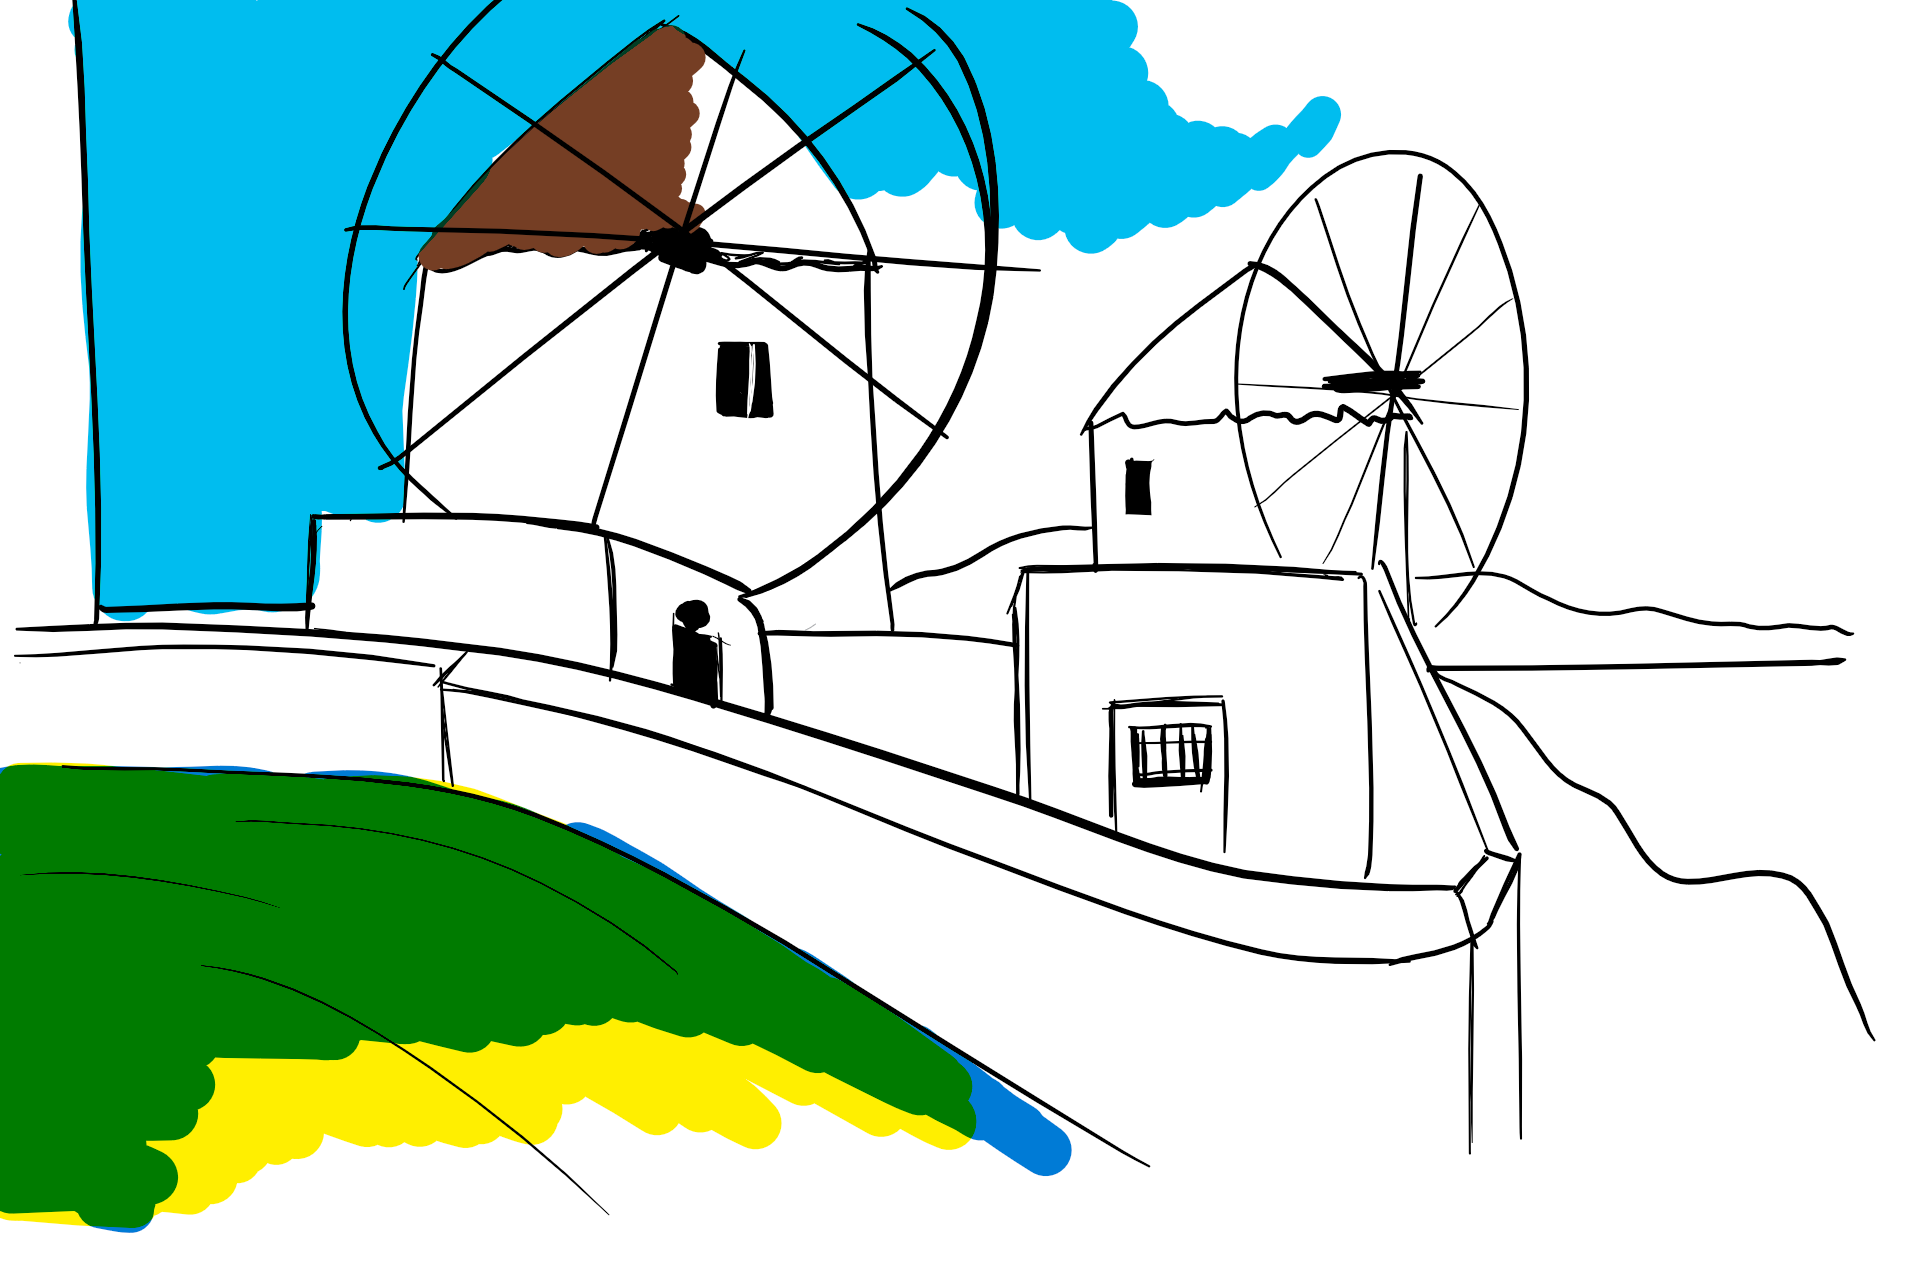
\includegraphics[width=.5\textwidth]{q.png}
\end{figure}}
% Feynman Diagram Setting
\usetikzlibrary{arrows.meta}
\newcommand{\midarrow}{\tikz \draw[-triangle 45] (0,0) -- +(.05,0);}
\tikzset{> = latex, color=blue}
\usetikzlibrary{decorations.markings,decorations.pathreplacing}
\tikzset{
	% style to apply some styles to each segment of a path
	on each segment/.style={draw=blue,
		decorate,
		    decoration={
			show path construction,
			moveto code={},
			lineto code={
				\path [#1]
				(\tikzinputsegmentfirst) -- (\tikzinputsegmentlast);
			},
			curveto code={
				\path [#1] (\tikzinputsegmentfirst)
				.. controls
				(\tikzinputsegmentsupporta) and (\tikzinputsegmentsupportb)
				..
				(\tikzinputsegmentlast);
			},
			closepath code={
				\path [#1]
				(\tikzinputsegmentfirst) -- (\tikzinputsegmentlast);
			},
		},
	},
	% style to add an arrow in the middle of a path
	mid arrow/.style={postaction={decorate,decoration={
				markings,
				mark=at position #1 with {\draw[arrows = {-Latex[width=0pt 7, length=5pt]}] (0pt,.0pt) -- (1.8pt,0pt);}
	}}},
	mid arrow/.default={.55},
	mid arrow seg/.style={postaction={on each segment={decorate,decoration={
				markings,
				mark=at position #1 with {\draw[arrows = {-Latex[width=0pt 7, length=5pt]}] (0pt,.0pt) -- (1.8pt,0pt);}}
	}}},
	mid arrow seg/.default={.55},
	% style to add an reverse arrow in the middle of a path
	mid reverse arrow/.style={postaction={decorate,decoration={
			markings,
			mark=at position .45 with {\draw[arrows = {-Latex[width=0pt 7, length=5pt]}] (1.8pt,.0pt) -- (0pt,0pt);}
	}}},
	mid reverse arrow seg/.style={postaction={on each segment={decorate,decoration={
				markings,
				mark=at position #1 with {\draw[arrows = {-Latex[width=0pt 7, length=5pt]}] (1.8pt,.0pt) -- (0pt,0pt);}}
	}}},
	above arrow/.style={to path={-- ++(0, .2) -| (\tikztotarget)},arrows = {-Latex[width=0pt 7, length=5pt]}},
	below arrow/.style={to path={-- ++(0,-.2) -| (\tikztotarget)}}
}
\newlength{\wletter}
\newlength{\hletter}
\newcommand{\tikzmark}[1]{
	\settowidth{\wletter}{\text{$\mathsurround=0pt i$}}
	\settoheight{\hletter}{\text{$\mathsurround=0pt i$}}
	\tikz[overlay,remember picture,inner sep=0,minimum height=\hletter] \node[shift={(-.4\wletter,.45\hletter)}] (#1) {};}
\newcommand{\dian}{\tikz{\filldraw[blue](0,0)circle(1pt);}}

\usetikzlibrary{calc}
%\usepackage[compat=1.1.0]{tikz-feynman}
\usepackage{float}
\renewcommand{\thefootnote}{\roman{footnote}} % Change the marks of footnotes to numbers
\usepackage{blkarray} %分块矩阵
\usepackage[bookmarksnumbered=true]{hyperref}


\usepackage{wasysym}
%For the symbol \CheckedBox
\usepackage{stackengine,scalerel}
\newcommand\DSquare{\ThisStyle{\ensurestackMath{%
			\stackinset{c}{}{c}{}{\scalebox{.5}{$\SavedStyle\blacksquare$}}
			{\SavedStyle\square}}}}
%For a filled box.
%CR: https://tex.stackexchange.com/questions/553834/is-there-a-intermediate-checkedbox-symbol-in-latex

%-----------------------------------------------------------------
%	Convinent abbreviations
%-----------------------------------------------------------------
\renewcommand{\normalsize}{\fontsize{8pt}{9.6pt}\selectfont}
\newcommand{\diagsize}{\fontsize{5pt}{6.6pt}\selectfont}
\newcommand{\cs}{a^\dagger}
\newcommand{\hd}{\mathrm{H}_2}
\newcommand{\hft}{Hartree-Fock}
\newcommand{\twoe}{r_{12}^{-1}}
\newcommand{\tp}{\tilde{\Phi}}
%\usepackage[symbol]{footmisc} 
\newcommand{\bfr}{\mathbf{r}}
\newcommand{\heh}{\mathrm{HeH}^+}
\newcommand{\au}{\,\mathrm{a.u.}}
\newcommand{\ts}{\mathscr{S}} %总自旋算符
\usepackage{xeCJKfntef} % the package containing the command \CJKuderline*{} for the \mci command
\newcommand{\mci}[1]{\CJKunderline*{#1}}
\newcommand{\phrase}[1]{\CJKunderline*{#1}}
%%为方便而定义的简单代替, 最后要全部换回来.
\newcommand{\jt}{\ket{\Phi_0}}
\newcommand{\hjt}{\ket{\Psi_0}}
\newcommand{\jtn}{\Phi_0}
\newcommand{\hjtn}{\Psi_0}

%Convenience commands defined by Hao
\newcommand{\mrm}{\mathrm}
\newcommand{\mbf}{\mathbf}
\newcommand{\mcr}{\mathscr}
\newcommand{\op}{\mathscr}
\newcommand{\bs}[2]{\ensuremath\left\{ \vec{#1}_{#2} \right\}}
\newcommand{\kbs}[1]{\ensuremath\left\{ \ket{#1} \right\}}
\newcommand{\bbs}[1]{\ensuremath\left\{ \bra{#1} \right\}}
\newcommand{\madj}[1]{\ensuremath{\mbf #1}^\dagger}
\newcommand{\oadj}[1]{\ensuremath{\op #1}^\dagger}
\newcommand{\tr}[1]{\ensuremath{\mrm{tr}}\,#1}
%\newcommand{\ket}[1]{\ensuremath\left\vert #1\right\rangle}
%\newcommand{\bra}[1]{\ensuremath\left\langle #1\right\vert}
\newcommand{\Langle}{\ensuremath\Big\langle}
\newcommand{\Rangle}{\ensuremath\Big\rangle}
\newcommand{\Lvert}{\ensuremath\Big\vert}
\newcommand{\olp}[2]{\ensuremath\langle #1 \vert #2 \rangle}
\newcommand{\Olp}[2]{\ensuremath\left\langle #1 \middle\vert #2 \right\rangle}
\newcommand{\oup}[2]{\ensuremath\left\vert #1 \right\rangle \left\langle #2 \right\vert}
\newcommand{\mele}[3]{\ensuremath\langle #1\vert \op{#2} \vert #3\rangle}
\newcommand{\Mele}[3]{\ensuremath\left\langle #1\middle\vert \op{#2} \middle\vert #3\right\rangle}
\newcommand\bigzero{\makebox(0,0){\text{\huge0}}}
%=============END===================



\date{\today}


\begin{document}
%\chapter*{修订版前言}
修订版与第一版相比, 有三处变化较大. 一是增加了附录. 
\chapter*{第一版前言}


\chapter*{进度表}

\makeatletter
\@date
\makeatother

\begin{itemize}
    \item[\CheckedBox] 第一章  数学预备
    \item[\CheckedBox] 第二章  多电子波函数与多电子算符
    \item[\DSquare] 第三章  Hatree-Fock近似 
    	\begin{itemize}
		    \item[\CheckedBox] 3.1-3.5
		    \item[\DSquare] 3.6 
		    	\begin{itemize}
		            \item[\CheckedBox] 3.6.1,3.6.2
		            \item[\Square] 3.6.3, 3.6.4
		        \end{itemize}
		    \item[\Square] 3.7
		    \item[\DSquare] 3.8 
			   \begin{itemize}
				     \item[\CheckedBox] 3.8.1-3.8.5
				     \item[\Square] 3.8.6
				     \item[\DSquare] 3.8.7
			   \end{itemize}
    	\end{itemize}
    \item[\DSquare] 
    	第四章 组态相互作用 
	    \begin{itemize}
	        \item[\DSquare] 4.1
	        \item[\CheckedBox] 4.2
			\item[\Square] 4.3
	        \item[\CheckedBox] 4.4
	        \item[\DSquare] 4.5
		\item[\Square] 4.6
	    \end{itemize}
    \item[\DSquare] 第五章 对理论与耦合对理论 
	    \begin{itemize}
	        \item[\DSquare] 5.1
	        \item[\DSquare] 5.2
	        \begin{itemize}
				\item [\CheckedBox] 5.2.1
				\item [\CheckedBox] 5.2.2
				\item [\Square] 5.2.3-5.2.4
			\end{itemize}
			\item[\Square] 5.3
	    \end{itemize}
    \item[\CheckedBox] 第六章 多体微扰论 
%	    \begin{itemize}
%	        \item[\CheckedBox] 6.1-6.8
%	        \item[\CheckedBox] 6.8 
%	    \end{itemize}
    \item[\DSquare] 单粒子多体格林函数 
    	\begin{itemize}
	        \item[\CheckedBox] 7.1-7.2
	        \item[\DSquare] 7.3
	        \item[\Square] 7.4-7.5 
    	\end{itemize}
    \item[\DSquare]  附录 \begin{itemize}
        \item[\CheckedBox] 附录A
        \item[\Square] 附录B
        \item[\Square] 附录C
        \item[\Square] 附录D
    \end{itemize}
\end{itemize}

\tableofcontents % Print the table of contents itself
\setcounter{page}{0}

%注意替换\ts -> \mathscr{S}, \cs _> a^\dagger, \sch -> Schr\''odinger, \hs 为\mathscr{H}, \vs -> \mathscr{V}, 算子 -> 算符. \ht
%
%!TEX root = ../main.tex
\chapter{数学知识复习}
\label{ch:1}

本章提供了阅读本书所需要的数学背景知识。
量子化学中最重要的数学工具是矩阵代数。
我们将本章设计为针对这样一类读者:
他们对矩阵有一些认识,但已经很长时间没有接触过,
而又希望能得到一些线性代数的知识和应用经验。
对于具有较强数学背景的读者,
可以快速浏览本章,
以便熟悉本书使用的符号和记号。
简单起见,我们牺牲了数学严格性,
采用了一种非正式的方式来讲述这部分内容。
为了帮助读者掌握这些非常重要但又经常被忽视的数学技巧,
我们在知识点讲述过程中插入了许多认真选择的习题。
完成这些简单的习题对于掌握本章内容来说是一个必要的过程。

第一节中,我们逐步将三维矢量代数中遇到的概念和结论推广到线性代数的基本概念,
包括:矩阵、行列式、线性算符及其矩阵表示、以及计算矩阵本征值和本征矢量的方法,
后者在量子化学中尤其重要。
我们介绍了 Dirac 符号,
这使得我们可以将这些结论表述为一种简洁、优美的形式。
更为有用的是,
我们可以利用 Dirac 符号操作矩阵,
并更容易的推导各种定理。
此外,这种符号体系还突显出线性代数和完备正交函数集理论的内在联系,
这一部分我们将在第二节中涉及到。
第三节介绍了变分原理,这是量子化学理论的基石之一。

\section{线性代数}
\label{sec:1.1}

我们通过复习三维空间的矢量代数来开启关于线性代数的讨论。
在本节以及本书其它部分中用到的教学技巧是,
以最简单的情形为例展示最基本的概念和思路,
然后将这些结果推广到更为复杂的情景中去。

\subsection{三维矢量代数}
\label{sec:1.1.1}
一个三维矢量可以通过指定它的分量 $a_i,\; i = 1, 2, 3$ 来描述,
这三个分量分别对应于三个互相垂直的单位矢量 $\{\vec{e}_i\}$:
\begin{equation}
\vec{a} = \vec{e}_1 a_1 + \vec{e}_2 a_2 + \vec{e}_3 a_3 = \sum_i \vec{e}_i a_i
\label{eq:1.1}
\end{equation} 
这三个矢量组成一组\emph{基}\index{基},
而它们本身则被称为\emph{基矢}。
如果任意一个三维矢量都可以写成这组基的线性组合,
则称这组基是完备的。
然而,基的选择不是唯一的;
我们可以选择其它三个互相垂直的单位矢量,
如 $\vec{\varepsilon}_i,\; i = 1, 2, 3$,
并将矢量 $\vec{a}$写作:
\begin{equation}
 \vec{a} = \vec{\varepsilon}_1 a^\prime_1 + \vec{\varepsilon}_2 a_2^\prime + \vec{\varepsilon}_3 a_3^\prime = \sum_i \vec{\varepsilon}_i a_i^\prime
 \label{eq:1.2}
\end{equation} 
给定一组基,
一个矢量可以通过指定它在该组基内的三个分量完全确定。
如,利用基组 $\{\vec{e}_i\}$,
我们可以将矢量 $\vec{a}$ 写作一个\emph{列矩阵}的形式:
\begin{subequations}
 \begin{equation}
     {\mbf a} = \left(
     \begin{array}{c} a_1 \\ a_2 \\ a_3 \end{array}
     \right)
     \label{eq:1.3a}
 \end{equation}
或者利用基组 $\{\vec{\varepsilon}_i\}$ 写成 
 \begin{equation}
     {\mbf a}^\prime = \left(
     \begin{array}{c}a_1^\prime \\ a_2^\prime \\ a_3^\prime\end{array}
     \right) 
     \label{eq:1.3b} 
 \end{equation}
\end{subequations}

两个矢量 $\vec{a}$ 和 $\vec{b}$ 的\emph{标积}或\emph{点积}定义为:
\begin{equation}
 \vec{a}\cdot\vec{b} = a_1 b_1 + a_2 b_2 + a_3 b_3 = \sum_i a_i b_i
 \label{eq:1.4}
\end{equation}
同时我们还注意到
\begin{equation}
 \vec{a}\cdot\vec{a} = a_1^2 + a_2^2 + a_3^2 \equiv \vert a\vert^2
 \label{eq:1.5}
\end{equation}
是矢量 $\vec{a}$ 的长度($\vert \vec{a}\vert$)的平方。
现在我们来看一下怎么利用\autoref{eq:1.1}计算标积 $\vec{a}\cdot\vec{b}$:
\begin{equation}
 \vec{a}\cdot\vec{b} = \sum_i\sum_j \vec{e}_i\cdot\vec{e}_j\, a_i b_j
 \label{eq:1.6}
\end{equation}
上式必须与\autoref{eq:1.4}相等,
因此,我们得到如下关系:
\begin{equation}
 \vec{e}_i \cdot \vec{e}_j = \delta_{ij} = \delta_{ji} = 
          \begin{cases}
           1 \quad \text{如果$i=j$} \\
                    0 \quad \text{其他情况}
 \end{cases}
 \label{eq:1.7}
\end{equation}
其中 $\delta_ij$ 为 Kronecker delta 函数。
上式是基矢\emph{正交归一}性质的数学描述:
基矢之间互相垂直(正交),
并且具有单位长度(归一)。 

给定一个矢量 $\vec{a}$,
我们利用正交归一关系\autoref{eq:1.7},
通过求算公\autoref{eq:1.1}与基矢 $\vec{e}_j$ 之间的标量积来得到它的三个分量:
\begin{equation}
 \vec{e}_j \cdot \vec{a} = \sum_i \vec{e}_j \cdot \vec{e}_i\, a_i = \sum_i \delta_{ji} a_i = a_j
 \label{eq:1.8}
\end{equation}
这样我们又可以将公\autoref{eq:1.1}写成如下形式:
\begin{equation}
 \vec{a} = \sum_i \vec{e}_i\vec{e}_i \cdot \vec{a} = \vec{1}\cdot\vec{a}
 \label{eq:1.9}
\end{equation}
其中
\begin{equation}
 \vec{1} = \sum_i \vec{e}_i \vec{e}_i
 \label{eq:1.10}
\end{equation}
为单位\emph{并矢}。
当一个并矢与一个矢量进行点乘操作时,
会得到一个新的矢量。
而单位并矢与矢量点乘则会得到原来的矢量。公\autoref{eq:1.10}被称作基组 $\{\vec{e}_i\}$ 的\emph{完备性关系}。
它其实是公\autoref{eq:1.1}的变形,
说明了任意矢量 $\vec{a}$ 都可以写作基矢
$\{\vec{e}_i\}$ 的线性组合这一事实。

现在我们对\emph{算符}进行定义:
算符 $\mcr{O}$ 可以作用在一个矢量 $\vec{a}$ 上,
将之转变成另一个矢量 $\vec{b}$:
\begin{equation}
 \mcr{O}\vec{a} = \vec{b}
 \label{eq:1.11}
\end{equation}
对于任意的数 $x$ 和 $y$,如果一个算符满足下述关系:
\begin{equation}
 \mcr{O}\left(x\vec{a} + y\vec{b}\right) = x\op{O}\vec{a} + y\op{O}\vec{b}
 \label{eq:1.12}
\end{equation}
则$\op{O}$为\emph{线性}算符。
我们可以通过检查线性算符作用在每个可能矢量上的结果来确定这个算符本身。
由于任意矢量都可以写成基组 $\{\vec{e}_i\}$ 的线性组合,
只需要知道 $\op{O}$ 作用在基矢上的效果就足以确定该算符。
我们知道 $\op{O}\vec{e}_i$ 是一个矢量,
它可以写作基矢 $\bs{e}{i}$ 的线性组合:
\begin{equation}
 \op{O}\vec{e}_i = \sum_{j=1}^3 \vec{e}_j O_{ji}, \quad i = 1, 2, 3
 \label{eq:1.13}
\end{equation}
$O_{ji}$是一个数,它是矢量$\op{O}\vec{e}_i$沿基矢$\vec{e}_j$的分量。
这九个分量可以写成一个\emph{矩阵}:
\begin{equation}
 \mbf{O} = \left(
 \begin{array}{ccc}
     O_{11} &O_{12} &O_{13} \\
     O_{21} &O_{22} &O_{23} \\
     O_{31} &O_{32} &O_{33} \\
 \end{array}
 \right)
 \label{eq:1.14}
\end{equation}
这里,$\mbf{O}$被称作算符$\op{O}$在基组$\bs{e}{i}$的\emph{矩阵表示}。
矩阵$\mbf{O}$完全确定了算符$\op{O}$的效果,
这是因为:
任一矢量都可以写成基矢$\bs{e}{i}$的线性组合的形式,
而算符$\op{O}$作用在每个基矢上的效果又为已知。

\exercise{
a) 证明 $O_{ij} = \vec{e}_i \cdot \op{O}\vec{e}_j$。
b) 若$\op{O}\vec{a} = \vec{b}$,证明$b_i = \sum_j O_{ij}a_j$。
}

如果矩阵$\mbf{A}$ 和$\mbf{B}$分别为算符$\op{A}$和$\op{B}$的矩阵表示, 
若算符$\op{C}$为$\op{A}$与$\op{B}$的乘积($\op{C} = \op{A}\op{B}$),
则$\op{C}$的矩阵表示可以通过如下方法得到:
\begin{equation}
 \begin{split}
 \op{C}\vec{e}_j &= \sum_i \vec{e}_i C_{ij} \\
 &= \op{A}\op{B} \vec{e}_j \\
 &= \op{A}\sum_k \vec{e}_k B_{kj} \\
 &= \sum_{ik} \vec{e}_i A_{ik}B_{kj}
 \end{split} 
 \label{eq:1.15}
\end{equation}
由此,我们得出:
\begin{equation}
 C_{ij} = \sum_k A_{ik}B_{kj}
 \label{eq:1.16}
\end{equation}
上式即为矩阵乘法的定义,因此,我们有:
\begin{equation}
 \mathbf{C} = \mathbf{A}\mathbf{B}
 \label{eq:1.17}
\end{equation}
这样,如果我们通过公\autoref{eq:1.16}定义矩阵的乘法,
则两个算符的乘积的矩阵表示即为这两个算符的矩阵表示的乘积。

在矩阵的乘法中,两个相乘算符的顺序非常重要。
通常情况下我们有 $\op{A}\op{B} \neq \op{B}\op{A}$,
或者 $\mathbf{A}\mathbf{B} \neq \mathbf{B}\mathbf{A}$,
即两个算符或两个矩阵并不一定是\emph{对易}的。
我们在此定义两个算符或矩阵的\emph{对易式},以供后面章节参考:
\begin{subequations}
 \begin{align}
     \left[\op{A}, \op{B}\right] &= \op{A}\op{B} - \op{B}\op{A} \\
     \left[{\mbf A}{\mbf B}\right] &= {\mbf A}{\mbf B} - {\mbf B}{\mbf A}
 \end{align}
 \label{eq:1.18}
\end{subequations}
此外,两个算符或矩阵的\emph{反对易式}为:
\begin{subequations}
 \begin{align}
     \left\{\op{A},\op{B}\right\} &= \op{A}\op{B} + \op{B}\op{A}\label{eq:1.19a} \\
     \left\{{\mbf A}{\mbf B}\right\} &= {\mbf A}{\mbf B} + {\mbf B}{\mbf A}\label{eq:1.19b}
 \end{align}\label{eq:1.19}
\end{subequations}

\exercise{
 已知:
\[
     {\mbf A} = 
     \begin{pmatrix*}[r]
      1 &1 &0 \\ 1 &\ \ 2 &2 \\ 0 &2 &-1
     \end{pmatrix*}
     \qquad
     {\mbf B} =
     \begin{pmatrix*}[r]
      1 & -1 & \ \ 1 \\ -1 & 0 & 0 \\ 1 & 0 & 1
     \end{pmatrix*}     
\]
 计算$\left[{\mbf A}, {\mbf B}\right]$ 和 $\left\{{\mbf A}, {\mbf B}\right\}$。
}


\subsection{矩阵}
\label{sec:1.1.2}
我们已经看到了$3\times 3$的矩阵是怎样从三维矢量代数中衍生出来,
并了解了怎样做矩阵之间的乘法,
本小节中我们会将把这些结论推广到更多维度的情形。
若有一系列复数$\left\{A_{ij}\right\}$,
具有有序的下标 $i = 1, 2, \dots, N$ 和 $j = 1, 2, \dots, M$,
则这些数可以看做一个矩阵 $\mbf A$的元素,
此矩阵有$N$行$M$列:
\begin{equation}
 \mbf{A} = 
 \begin{pmatrix*}[c]
     A_{11} &A_{12} &\dots &A_{1M} \\
     A_{21} &A_{22} &\dots &A_{2M} \\
     \vdots &\vdots &               &\vdots \\
     A_{N1} &A_{N2} &\dots &A_{NM}
 \end{pmatrix*}
 \label{eq:1.20}
\end{equation}
如果 $N=M$,则此矩阵为方阵。
如果$N\times M$的矩阵$\mbf A$的列数与$M\times P$的矩阵$\mbf B$的行数相等,
则矩阵 $\mathbf{A}$和$\mbf B$可以相乘,
其结果为$N\times P$的矩阵$\mbf C$:
\begin{equation}
 \mbf{C} = \mbf{A}\mbf{B}
 \label{eq:1.21}
\end{equation}
其中$\mbf C$的元素由矩阵乘法法则确定:
\begin{equation}
 C_{ij} = \sum_{k=1}^M A_{ik}B_{kj}\qquad 
 \begin{array}{c}
     i = 1, \dots, N \\
     j = 1, \dots, M
 \end{array}
 \label{eq:1.22}
\end{equation}

$M$个数的集合$\left\{a_i\right\}, i = 1, 2, \dots, M$可以类似地看做一个列矩阵的元素:
\begin{equation}
 \mbf a = 
 \begin{pmatrix*}[c]
     a_1 \\ a_2 \\ \vdots \\ a_M
 \end{pmatrix*}
 \label{eq:1.23}
\end{equation}
对于一个$N\times M$的矩阵$\mbf A$,我们有:
\begin{equation}
 \mbf A \mbf a = \mbf b
 \label{eq:1.24}
\end{equation}
此处 $\mbf b$为一个具有$N$个元素的列矩阵,其元素为:
\begin{equation}
 b_i = \sum_{j=1}^M A_{ij}a_j \qquad i = 1, 2, \dots, N
 \label{eq:1.25}
\end{equation}

下面我们将介绍一些重要的定义。
一个$N\times M$矩阵 $\mbf A$的\emph{伴随矩阵},
记为$\mbf{A}^\dagger$,是一个$M \times N$的矩阵,其元素为:
\begin{equation}
 \left(\mbf{A}^\dagger\right)_{ij} = A_{ji}^{\ast}
 \label{eq:1.26}
\end{equation}
即对矩阵$\mbf A$的每个元素取复共轭,
并交换矩阵的行和列。
如果$\mbf A$为实矩阵,
则其伴随矩阵称为$\mbf A$的\emph{转置}。

\exercise{
 若$\mbf A$为维度$N \times M$的矩阵,$\mbf B$为$M \times K$矩阵,证明$\left( \mbf{A} \mbf{B} \right)^{\dagger} = \mbf{B}^\dagger \mbf{A}^\dagger$。
}

一个列矩阵的伴随矩阵为一个\emph{行矩阵},
其元素为原矩阵元素的复共轭:
\begin{equation}
 {\mbf a}^{\dagger} = 
 \begin{pmatrix*}[c]
     a_1^\ast & a_2^\ast &\dots &a_M^\ast
 \end{pmatrix*}
 \label{eq:1.27}
\end{equation}
如果${\mbf a}$和$\mbf b$均为含有$M$个元素的列矩阵,则有:
\begin{equation}
 {\mbf a}^{\dagger}{\mbf b} = 
 \begin{pmatrix*}[c]
     a_1^\ast & a_2^\ast &\dots &a_M^\ast
 \end{pmatrix*}
 \begin{pmatrix*}[c]
     b_1 \\ b_2 \\ \vdots \\ b_M
 \end{pmatrix*}
     = \sum_{i=1}^M a_i^{\ast} b_i
 \label{eq:1.28}
\end{equation}
通过与\autoref{eq:1.4}相比,
我们注意到,如果$\mbf a$和$\mbf b$均为实矩阵且$M$值为3时,
上式即为两个三维矢量的标量积。
对\autoref{eq:1.24}两边分别取其伴随矩阵,
并引用练习~\autoref{ex:1.3} 的结论,
我们得到如下关系:
\begin{equation}
 {\mbf b}^\dagger = {\mbf a}^\dagger {\mbf A}^\dagger
\end{equation}
此处$\madj{b}$是一个具有 $N$ 个元素的行矩阵:
\begin{equation}
 b_i^\ast = \sum_{j=1}^M a_j^\ast \left(\madj{A}\right)_{ji} = \left(
     \sum_{j=1}^M a_j A_{ij}
 \right)^\ast
 \label{eq:1.30}
\end{equation}
我们看到\autoref{eq:1.30}和\autoref{eq:1.25}互为复共轭。

下面我们直接给出关于\emph{方阵}的一些定义和性质:
\begin{enumerate}
 \item 若矩阵$\mbf A$的非对角元全为零,则称$\mbf A$为\emph{对角}阵:
 \begin{equation}
     A_{ij} = A_{ii}\delta_{ij}
     \label{eq:1.31}
 \end{equation}
 
 \item 矩阵$\mbf A$的\emph{秩}是其全部对角元的加和:
 \begin{equation}
     \tr{\mbf A} = \sum_i A_{ii}
     \label{eq:1.32}
 \end{equation}
 
 \item \emph{单位}矩阵的定义为,对任意矩阵$\mbf A$,如下关系成立:
 \begin{equation}
     {\mbf 1} {\mbf A} = {\mbf A}{\mbf 1} = {\mbf A}
     \label{eq:1.33}
 \end{equation}
 单位阵的元素为:
 \begin{equation}
     \left(\mbf 1\right)_{ij} = \delta_{ij}
     \label{eq:1.34}
 \end{equation}
 
 \item 矩阵$\mbf A$的\emph{逆矩阵}记为${\mbf A}^{-1}$,满足如下关系:
 \begin{equation}
     {\mbf A}^{-1}{\mbf A} = {\mbf A}{\mbf A}^{-1} = {\mbf 1}
     \label{eq:1.35}
 \end{equation}
 
 \item 若矩阵$\mbf A$的逆矩阵与其伴随矩阵相等,则$\mbf A$为\emph{幺正}矩阵:
 \begin{equation}
     {\mbf A}^{-1} = \madj{A}
     \label{eq:1.36}
 \end{equation} 
 一个实幺正矩阵被称为\emph{正交}阵。
 
 \item 自伴随矩阵称为\emph{Hermitian}矩阵,即:
 \begin{subequations}
     \begin{equation}
     \madj{A} = {\mbf A} \\
     \label{eq:1.37a}
     \end{equation}
     或者
     \begin{equation}
      A_{ji}^\ast = A_{ij}
      \label{eq:1.37b}
     \end{equation}
 \end{subequations}
 实Hermitian矩阵被称为\emph{对称}矩阵。
\end{enumerate}

\exercise{
 证明下述关系:
 \begin{enumerate}[1.]
    \item $\tr{\mbf{AB}} = \tr{\mbf{BA}}$
    \item $\left(\mbf{AB}\right)^{-1} = {\mbf B}^{-1}{\mbf A}^{-1}$
    \item 设$\mbf B$为幺正,且有关系${\mbf B} = \madj{U}{\mbf A}{\mbf U}$,则有${\mbf A} = {\mbf U}{\mbf B}{\madj U}$。
    \item 若两个Hermitian矩阵${\mbf A}$和${\mbf B}$的乘积${\mbf C} = \mbf{AB}$也是Hermitian矩阵,则${\mbf A}$和${\mbf B}$对易。
    \item 设${\mbf A}$为Hermitian矩阵,如果它的逆${\mbf A}^{-1}$存在,则逆矩阵也是Hermitian矩阵。
    \item 如果
        \[ {\mbf A} = 
        \begin{pmatrix}
            A_{11} & A_{12} \\ A_{21} & A_{22}
        \end{pmatrix} \]
    则有
    \[ {\mbf A}^{-1} = \frac{1}{\left(A_{11}A_{22} - A_{12}A_{21}\right)}
     \begin{pmatrix*}[r]
        A_{22} & -A_{12} \\ -A_{21} & A_{11}
    \end{pmatrix*} \]
 \end{enumerate}
}

\subsection{行列式}
\label{sec:1.1.3}
本小节中,我们将介绍方阵的行列式的性质。
我们知道关于$1, 2, 3, \dots, N$这$N$个数的一个\emph{排列},
就是将这些数排序的一种方式,
而这些数共有 $N!$种不同的排列方式。
一个$N\times N$的矩阵 $\mbf A$ 的\emph{行列式}是一个数,
它的值通过下式求得:
\begin{equation}
 \det{\mbf A} = \vert {\mbf A} \vert = \begin{vmatrix}
     A_{11} &\dots &A_{1N} \\ \vdots & &\vdots \\ A_{N1} &\vdots &A_{NN} 
 \end{vmatrix} = \sum_{i=1}^{N!} \left(-1\right)^{p_i}\op{P}_iA_{11}A_{22}\cdots A_{NN}
 \label{eq:1.38}
\end{equation}
其中$\op{P}_i$是排列算符,
它的作用是对连乘中各元素列下标进行排列,
上式的加和共有$N!$项;
$p_i$为由标准排列 $1, 2, 3, \dots, N$ 到一个给定的排列 $i_1, i_2, \dots, i_N$ 所需要的交换次数。
需要注意的是,
我们仅关心$p_i$是奇数还是偶数。
下面我们通过一个$2 \times 2$的矩阵来演示行列式的计算。
\[{\mbf A} = \begin{pmatrix}
 A_{11} & A_{12} \\ A_{21} & A_{22}
\end{pmatrix}\]
对于列下标$1$和$2$,我们有两种排列方式,即:
\[
1 \quad 2 \quad \left(p_1 = 0\right)\]\[
2 \quad 1 \quad \left(p_2 = 1\right)\]
因此,
\begin{equation}
 \begin{vmatrix}
     A_{11} & A_{12} \\ A_{21} &A_{22}
 \end{vmatrix} = \left(-1\right)^0 A_{11}A_{12} + \left(-1\right)^1 A_{12}A_{21} = A_{11}A_{12} - A_{12}A_{21}
 \label{eq:1.39}
\end{equation}
由这些定义,我们可以得出以下关于行列式的重要性质:
\begin{enumerate}
 \item 如果一个行列式的一行或一列全为零,则行列式的值为零。
 \item 如果${\mbf A}_{ij} = A_{ii}\delta_{ij}$,则$\vert A\vert = \prod_i A_{ii} = A_{11}A_{22}\cdots A_{NN}$。
 \item 交换行列式的两行或两列,行列式的值变号。
 \item $\vert \mbf{A} \vert = \left(\vert\madj{A}\vert\right)^\ast$ .
 \item $\vert {\mbf{AB}}\vert = \vert{\mbf A}\vert\vert\mbf{B}\vert$ .
\end{enumerate}

\exercise{
 用一个$2\times 2$的行列式做例子,验证上述行列式的性质。
\Next
 应用上述行列式性质,证明以下关系成立:
 \begin{enumerate}
     \item 如果行列式的两行或两列相等,则行列式的值为零。
     \item $\vert\mbf{A}^{-1}\vert = \left(\vert\mbf{A}\vert\right)^{-1}$
     \item 如果${\mbf A}{\madj A} = {\mbf 1}$,则$\vert{\mbf A}\vert\left(\vert\mbf{A}\vert\right)^{\ast} = \mbf{1}$。
     \item 如果 $\madj{U}{\mbf O}{\mbf U} = \boldsymbol{\Omega}$和$\madj{U}{\mbf U} = \mbf{U}\madj{U} = \mbf 1$,则有 $\vert \mbf{O}\vert = \vert\mathbf{\Omega}\vert$。
 \end{enumerate}
\Next
 对照\autoref{eq:1.39},
 我们发现在练习 \autoref{ex:1.4}f 中得到的$2\times 2$矩阵 $\mbf A$的逆可以写作:
 \[{\mbf A}^{-1} = \frac{1}{\vert\mbf{A}\vert}
 \begin{vmatrix*}[r]
     A_{22} & -A_{12} \\ -A_{21} & A_{11}
 \end{vmatrix*}
 \]
 由此看到,如果$\vert\mbf{A}\vert = 0$,
 则$\vert\mbf{A}\vert^{-1}$不存在。
 这个结论对于$N\times N$维的矩阵也成立。
 验证如下方程:
 \[{\mbf A}{\mbf c} = 0\]
 有非平凡解($\mbf{c}\neq 0$)的必要条件是 $\vert\mbf{A}\vert = 0$。
 其中,$\mbf A$为$N\times N$矩阵,
 $\mbf c$为列矩阵,
 其元素为$c_i,\; i = 1, 2, \dots, N$。
}

对于$2\times 2$行列式,很容易通过直接求算来验证如下关系:
\[
\begin{vmatrix}
 c_1B_{11} + c_2B_{12} & A_{12} \\ c_1B_{21} + c_2B_{22} & A_{22}
\end{vmatrix} = 
c_1 \begin{vmatrix}
 B_{11} & A_{12} \\ B_{21} & A_{22}
\end{vmatrix} + 
c_2 \begin{vmatrix}
 B_{12} & A_{12} \\ B_{22} & A_{22}
\end{vmatrix}
\]
这是 N 维行列式性质的一个特殊情形,
本书后面内容将多次用到行列式的这个性质:
\begin{equation}
 \begin{split}
 \begin{vmatrix}
     A_{11} & A_{12} &\cdots &\displaystyle\sum_{k=1}^M c_kB_{1k} &\cdots &A_{1N} \\ 
     A_{11} & A_{22} &\cdots &\displaystyle\sum_{k=1}^M c_kB_{2k} &\cdots &A_{2N} \\ 
     \vdots &\                &\           &\                                                       &\vdots \\
     A_{11} & A_{N2} &\cdots &\displaystyle\sum_{k=1}^M c_kB_{Nk} &\cdots &A_{NN}
 \end{vmatrix}\qquad \\
 \qquad = \sum_{k=1}^{M} c_k \begin{vmatrix}
     A_{11} & A_{12} &\cdots      &B_{1k}     & \cdots      & A_{1N} \\
     A_{21} & A_{22} &\cdots      &B_{2k}     & \cdots     & A_{2N} \\
     \vdots &\vdots     &\               &\vdots      &\          &\vdots \\
     A_{N1} & A_{N2} &\cdots      &B_{Nk}     & \cdots      & A_{NN} \\
 \end{vmatrix}
 \end{split}
 \label{eq:1.40}
\end{equation}
对于行存在加和的情形,也有一个类似的结论。

\subsection{N 维复矢量空间}
\label{sec:1.1.4}
下面我们将在三维矢量代数中用到的方法和得到的结论推广到$N$维空间,
并且此时矢量可以为复数。
我们将开始使用 Dirac 符号,
这是一套强有力的符号体系,
可以简洁地表述我们得到的结论。
与三维空间的基组$\bs{e}{i}$类似,
在$N$维空间中,
我们把$N$个基矢量标记为 $\ket{i},\; i = 1, 2, \dots, N$。
这些基矢被称为\emph{右矢量}或\emph{右矢}。我
们总是可以选择一套完备的基矢,
从而可以将 $N$维空间中的任意右矢 $\ket{a}$写为如下形式:
\begin{equation}
 \ket{a} = \sum_{i=1}^{N} \ket{i} a_i
 \label{eq:1.41}
\end{equation}
上式是\autoref{eq:1.1}的简单推广,
不过这里我们用到了新引入的 Dirac 符号。
指定基组以后,
我们可以通过给出矢量沿$N$个基矢$\left\{\ket{i}\right\}$的组份$a_i$来完全描述这个矢量,
其中$i = 1, 2, \dots, N$。
同样,我们还可以将这些分量写到列矩阵里面:
\begin{equation}
 {\mbf a} = \begin{pmatrix}
     a_1 \\ a_2 \\ \vdots \\ a_N
 \end{pmatrix}
 \label{eq:1.42}
\end{equation}
这里 $\mbf a$是抽象的矢量 $\ket{a}$在基组 $\left\{\ket{i}\right\}$ 中的矩阵表示。
\autoref{eq:1.27}提到,
一个列矩阵$\mbf a$的伴随矩阵$\madj{a}$是一个行矩阵:
\begin{equation}
 \madj{a} = \begin{pmatrix}
     a_1^\ast & a_2^\ast &\cdots &a_N^\ast
 \end{pmatrix}
 \label{eq:1.43}
\end{equation}
这里我们引入另一个抽象的矢量\emph{左矢} $\bra{a}$,
它的矩阵表示为 $\madj{a}$。
左矢$\bra{a}$和右矢$\ket{b}$之间的标量积定义为:
\begin{equation}
 \bra{a}\ket{b} \equiv \olp{a}{b} = \madj{a}\mbf{b} = \begin{pmatrix}
     a_1^\ast & a_2^\ast &\cdots &a_N^\ast
 \end{pmatrix} \begin{pmatrix}
     b_1 \\ b_2 \\ \vdots \\ b_N
 \end{pmatrix} = \sum_{i=1}^N a_i^\ast b_i
 \label{eq:1.44}
\end{equation}
上式同样是\autoref{eq:1.4}的简单推广。
左矢和右矢的英文名分别为 bra ($\bra{\ }$) 和 ket($\ket{\ }$),
来自于它们的标量积表达式($\olp{\ }{\ }$)形似括号(bra-c-ket)。
我们还注意到
\begin{equation}
 \olp{a}{a} = \sum_{i=1}^N a_i^\ast a_i = \sum_{i=1}^N \vert a_i\vert^2
 \label{eq:1.45}
\end{equation}
只能取正实数值,是三维矢量的长度平方的一个推广。
类似于\autoref{eq:1.41},
我们还可以引入一套完备的左基组$\bbs{i}$,
这样可以将任意的左矢 $\bra{a}$写为左基矢的线性组合:
\begin{equation}
 \bra{a} = \sum_i a_i^\ast \bra{i}
 \label{eq:1.46}
\end{equation}
这时矢量$\bra{a}$ 和$\ket{b}$的标量积可以表述为:
\[
\olp{a}{b} = \sum_{ij}a_i^\ast \olp{i}{j} b_j
\]
上式应与\autoref{eq:1.44}中关于标量积的定义等同,因此,我们有:
\begin{equation}
 \olp{i}{j} = \delta_{ij}
 \label{eq:1.47}
\end{equation}
此式是\autoref{eq:1.7}在$N$维空间的推广,
描述了基矢的正交归一性。
总之,我们可以将右矢$\ket{a}$写为列矩阵$\mbf a$的形式,
可以将左矢$\bra{b}$写为行矩阵$\madj{b}$的形式,
它们的标量积则可以写成各自矩阵表示的矩阵乘积。

现在想一下,给定一个右矢 $\ket{a}$或一个左矢$\bra{a}$,
怎样才能得到它在基组$\kbs{i}$或$\bbs{i}$中的各个分量呢?
下面我们将完全参照三维情形[\autoref{eq:1.8}]来完成这一步:
把\autoref{eq:1.41}从左边乘$\bra{j}$,
\autoref{eq:1.46}从右边乘$\ket{j}$,
这样我们有:
\begin{subequations}
 \begin{equation}
     \olp{j}{a} = \sum_i\olp{j}{i}a_i = \sum_i \delta_{ji}a_i = a_j
     \label{eq:1.48a}
 \end{equation}
以及
 \begin{equation}
     \olp{a}{j} = \sum_i a_i^\ast \olp{i}{j} = \sum_i a_i^\ast\delta_{ij} = a_j^\ast
     \label{eq:1.48b}
 \end{equation}
\end{subequations}
这里我们提到的``方程两边从左边乘$\bra{j}$''是``分别求取方程两边与$\bra{j}$的标量积''的简便说法。
我们还注意到
\begin{equation}
 \olp{j}{a} = \left(\olp{a}{j}\right)^\ast = \olp{a}{j}^\ast
 \label{eq:1.49}
\end{equation}
利用这个结果可以将\autoref{eq:1.41}和\autoref{eq:1.46}写成如下形式:
\begin{subequations}
 \begin{equation}
     \ket{a} = \sum_i \ket{i}a_i = \sum_i \ket{i}\olp{i}{a}
     \label{eq:1.50a}
 \end{equation}
以及
 \begin{equation}
     \bra{a} = \sum_i a_i^\ast\bra{i} = \sum_i \olp{a}{i}\bra{i}
     \label{eq:1.50b}
 \end{equation}
\end{subequations}
从上面两式可以得到:
\begin{equation}
 \mbf{a} = \sum_i \ket{i}\bra{i}
 \label{eq:1.51}
\end{equation}
即为$N$维空间基组的完备性关系,
是\autoref{eq:1.10}的推广。
我们将会发现,
在很多公式推导中插入完备性关系是一个非常有用的方法。

与公\autoref{eq:1.11}类似,
我们通过作用在右矢上的效果来定义算符:
算符$\op{O}$作用在右矢$\ket{a}$上,
将之转变成右矢$\ket{b}$
\begin{equation}
 \op{O}\ket{a} = \ket{b}
 \label{eq:1.52}
\end{equation}
与三维情形相同,
一旦能够确定算符作用在基组上的效果,
这个算符就完全确定了,
\begin{equation}
 \op{O}\ket{i} = \sum_j\ket{j}O_{ji} = \sum_j\ket{j}\left(\mbf{O}\right)_{ji}
 \label{eq:1.53}
\end{equation}
这里$\mbf O$是算符$\op{O}$在基组$\kbs{i}$内的矩阵表示。
将\autoref{eq:1.53}式从左边乘$\bra{k}$,我们得到:
\begin{equation}
 \Mele{k}{O}{i} = \sum_j\olp{k}{j}\left(\mbf O\right)_{ji} = \sum_j\delta_{kj} \left(\mbf O\right)_{ji} = \left(\mbf O\right)_{ki}
 \label{eq:1.54}
\end{equation}
上式即为$\mbf O$的矩阵元的表达式。
需要注意的是,借助完备性关系\autoref{eq:1.51},
我们也可以容易地通过以下方法得到算符$\op{O}$的矩阵表示:
\begin{equation}
 \op{O}\ket{i} = {\mbf 1}\op{O}\ket{i} = \sum_j\ket{j}\Mele{j}{O}{i}
 \label{eq:1.55}
\end{equation}
上式与\autoref{eq:1.53}相比,我们有:
\begin{equation}
 \Mele{j}{O}{i} = \left(\mbf O\right)_{ji} = O_{ji}
 \label{eq:1.56}
\end{equation}
下面我们通过另一个例子来展示完备性关系以及 Dirac 符号内禀的简明和一致性的应用:
已知算符$\op{A}$和$\op{B}$的矩阵表示,推导他们的乘积$\op{C} = \op{A}\op{B}$的矩阵表示。
\[
\begin{split}
 \Mele{i}{C}{j} = \left(\mbf C\right)_{ij} = \Mele{i}{AB}{j} &= \left\langle i\middle\vert\op{A}\mbf{1}\op{B}\middle\vert j\right\rangle \\
 &= \sum_k \Mele{i}{A}{k} \Mele{k}{B}{j} \\
 &= \sum_k \left(\mbf A\right)_{ik} \left(\mbf B\right)_{kj}
\end{split}
\]

算符$\op{O}$的\emph{伴随}算符标记为$\oadj{O}$。
如果算符$\op{O}$作用在右矢$\ket{a}$上将之转变成$\ket{b}$,
则其伴随算符将左矢$\bra{a}$转变成$\bra{b}$:
\begin{equation}
 \bra{a}\oadj{O} = \bra{b}
 \label{eq:1.57}
\end{equation}
上式与\autoref{eq:1.52}互为伴随。
在\autoref{eq:1.52}两边同左乘$\bra{c}$,
\autoref{eq:1.57}两边同右乘$\ket{c}$,我们得到:
\[
\Mele{c}{O}{a} = \olp{c}{b}
\]
以及
\[
\left\langle a\middle\vert \oadj{O}\middle\vert c\right\rangle = \olp{b}{c}
\]
由于$\olp{b}{c} = {\olp{c}{b}}^\ast$,如下关系成立:
\begin{equation}
 \left\langle a\middle\vert \oadj{O}\middle\vert c\right\rangle = {\Mele{c}{O}{a}}^\ast
 \label{eq:1.58}
\end{equation}
由于$a, b$和$c$为任意矢量,
这样我们就证明了算符$\oadj{O}$的矩阵表示与算符$\op{O}$的矩阵表示的伴随矩阵相等:
\begin{equation}
 \left\langle i\middle\vert \oadj{O}\middle\vert j\right\rangle \equiv \left(\mbf{O}^\dagger\right)_{ij} = {\Mele{j}{O}{i}}^\ast \equiv O_{ji}^\ast
 \label{eq:1.59}
\end{equation}
在本小节最后,我们介绍一下Hermitian算符,即自伴算符:
\begin{equation}
 \op{O} = \oadj{O}
 \label{eq:1.60}
\end{equation}
Hermitian算符矩阵表示的矩阵元满足如下关系:
\begin{equation}
 \Mele{a}{O}{b} = \left\langle a\middle\vert \oadj{O}\middle\vert b\right\rangle = {\Mele{b}{O}{a}}^\ast
 \label{eq:1.61}
\end{equation}


\subsection{基组变换}
\label{sec:1.1.5}
在\autoref{sec:1.1.1}中,
我们知道了基组的选择不是唯一的。
给定两个完备的正交归一基组$\kbs{i}$和$\kbs{\alpha}$,
本小节中我们将找出他们之间的关系。
我们把第一个基组下左矢和右矢用拉丁字母$i, j, k, \dots$标记;
第二个基组下的矢量用希腊字母$\alpha, \beta, \gamma, \dots$标记。
这样,我们有:
\begin{subequations}
 \begin{equation}
     \olp{i}{j} = \delta_{ij}, \qquad\sum_i \oup{i}{i} = 1
     \label{eq:1.62a}
 \end{equation}
以及
\begin{equation}
 \olp{\alpha}{\beta} = \delta_{\alpha\beta}, \qquad \sum_{\alpha}\oup{\alpha}{\alpha} = 1
 \label{eq:1.62b}
\end{equation}
\end{subequations}
由于基组$\kbs{i}$是完备的,
我们可以将基组$\kbs{\alpha}$中的任一基矢$\ket{\alpha}$展开为基组$\kbs{i}$中基矢的线性组合,
反之亦然。即:
\begin{equation}
 \ket{\alpha} = 1\ket{\alpha} = \sum_i\ket{i}\olp{i}{\alpha} = \sum_i \ket{i}U_{i\alpha} = \sum_i \ket{i}\left(\mbf U\right)_{i\alpha}
 \label{eq:1.63}
\end{equation}
其中,变换矩阵$\mbf U$的矩阵元定义为:
\begin{equation}
 \olp{i}{\alpha} = U_{i\alpha} = \left(\mbf U\right)_{i\alpha}
 \label{eq:1.64}
\end{equation}
对于反向的变换,我们有:
\begin{equation}
 \ket{i} = 1\ket{i} = \sum_{\alpha}\ket{\alpha}\olp{\alpha}{i} = \sum_{\alpha} \ket{\alpha}U_{i\alpha}^\ast = \sum_{\alpha} \ket{\alpha}\left(\madj{U}\right)_{\alpha i}
 \label{eq:1.65}
\end{equation}
上式中我们用到了\autoref{eq:1.49}和伴随矩阵的定义,
从而得到如下关系:
\begin{equation}
 \olp{\alpha}{i} = {\olp{\alpha}{i}}^\ast = U_{i\alpha}^\ast = \left(\madj{U}\right)_{\alpha i}
 \label{eq:1.66}
\end{equation}
此处有一个要点需要记住,
由于我们用\autoref{eq:1.64}定义了变换矩阵$\mbf U$,则$\olp{\alpha}{i} \neq U_{\alpha i}$,
而要用\autoref{eq:1.66}计算。
下面我们证明$\mbf U$是一个幺正矩阵,
这是基组的正交归一性导致的:
\[
\begin{split}
\delta_{ij} &= \olp{i}{j} \\
&= \sum_{\alpha}\olp{i}{\alpha}\olp{\alpha}{j} \\
&= \sum_{\alpha}\left(\mbf U\right)_{i\alpha}\left(\mbf U\right)_{\alpha j} \\
&= \left(\mbf{U}\madj{U}\right)_{ij}
\end{split}
\]
如果采用矩阵符号,上式可以写为:
\begin{subequations}
 \begin{equation}
     \mbf 1 = \mbf{U} \madj{U}
     \label{eq:1.67a}
 \end{equation}
类似的,还可以从$\olp{\alpha}{\beta} = \delta_{\alpha\beta}$出发,得到:
\begin{equation}
 \mbf 1 = \madj{U}\mbf{U}
 \label{eq:1.67b}
\end{equation}
\end{subequations}
由此我们证明了$\mbf U$是一个幺正矩阵。
这样,我们得到了一个重要结论:
两个正交归一基组之间通过一个幺正矩阵相关,
可以通过该矩阵由一个基组变换至另一基组,
如\autoref{eq:1.63},
或者通过\autoref{eq:1.65}变换回至原基组;
这个幺正变换矩阵的矩阵元即为两个基组中基矢的标量积,
可通过\autoref{eq:1.64}计算。

下面我们考虑在不同的基组下,
算符 $\op{O}$ 的矩阵表示具有什么样的联系。
下一步我们得到的结果将在下一小节关于本征值问题的讨论中占据着中心地位。
假设$\mbf O$是算符$\op{O}$在基组$\kbs{i}$中的矩阵表示,
而$\boldsymbol{\Omega}$是该算符在基组$\kbs{\alpha}$中的矩阵表示,
则有:
\begin{subequations}
 \begin{equation}
     \op{O}\ket{i} = \sum_j \ket{j}\Mele{j}{O}{i} = \sum_j\ket{j}O_{ji}
     \label{eq:1.68a}
 \end{equation}
 \begin{equation}
     \op{O}\ket{\alpha} = \sum_{\beta} \ket{\beta}\Mele{\beta}{O}{\alpha} = \sum_{\beta} \ket{\beta}\Omega_{\beta\alpha}
     \label{eq:1.68b}
 \end{equation}
\end{subequations}
为了得到$\mbf O$和$\boldsymbol\Omega$之间的关系,
我们可以使用已经熟悉的技巧,
即在合适的位置插入单位算符:
\begin{equation}
 \begin{split}
     \Omega_{\alpha\beta} = \Mele{\alpha}{O}{\beta} &= \left\langle\alpha\middle\vert 1\op{O}1\middle\vert\beta\right\rangle \\
     &= \sum_{ij}\olp{\alpha}{i}\Mele{i}{O}{j}\olp{j}{\beta} \\
     &= \sum_{ij}\left(\madj{U}\right)_{\alpha i}\left(\mbf O\right)_{ij}\left(\mbf{U}\right)_{j\beta}
 \end{split}
 \label{eq:1.69}
\end{equation}
即为:
\begin{subequations}
 \begin{equation}
     \boldsymbol\Omega = \madj{U}\mbf{O}\mbf{U}
     \label{eq:1.70a}
 \end{equation}
或者在上式两边左乘$\mbf U$,右乘$\madj{U}$,得到:
\begin{equation}
 \mbf O = \mbf{U}\boldsymbol\Omega\madj{U}
 \label{eq:1.70b}
\end{equation}
\end{subequations}
上述方程说明,
矩阵$\mbf{O}$和$\boldsymbol\Omega$可以通过一个\emph{幺正变换}联系起来。
幺正变换的重要性在于:对于任意的Hermitian算符,
若它在基组$\kbs{i}$中的矩阵表示不是对角的,
则总能找到一个基组$\kbs{\alpha}$,
使得在新基组中其矩阵表示为对角阵。即:
\begin{equation}
 \Omega_{\alpha\beta} = \omega_{\alpha}\delta_{\alpha\beta}
 \label{eq:1.71}
\end{equation}
在下一小节中,我们将要考虑怎样通过幺正变换将Hermitian矩阵对角化。

\exercise{
 证明:幺正变换后,矩阵的秩不变。
 即,若
 \[\boldsymbol\Omega = \madj{U}\mbf{O}\mbf{U}\]
 则有 $\tr{\boldsymbol\Omega} = \tr{\mbf O}$
}


\subsection{本征值问题}
\label{sec:1.1.6}
算符$\op{O}$作用在一个矢量$\ket{a}$上,
会得到一个新的矢量$\op{O}\ket{a}$。
通常情况下,这个新的矢量与原矢量不同。
如果$\op{O}\ket{a}$与$\ket{a}$只差一个常数,即:
\begin{equation}
 \op{O}\ket{a} = \omega_{\alpha}\ket{a}
 \label{eq:1.72}
\end{equation}
这时,我们可以称$\ket{a}$为算符$\op{O}$关于\emph{本征值} $\omega_{\alpha}$ 的\emph{本征矢量}。将本征矢归一化并不失普遍性:
\begin{equation}
 \olp{\alpha}{\alpha} = 1
 \label{eq:1.73}
\end{equation}
在本书中,我们关心的是Hermitian算符($\op{O}=\oadj{O}$)的本征矢和本征值。它们具有如下性质:
\begin{enumerate}[]
 \item {\bfseries Hermitian算符的本征值为实数。} 这个结论可以从\autoref{eq:1.61}直接得到:
 \begin{equation}
     \Mele{\alpha}{O}{\alpha} = \left\langle\alpha\middle\vert\op{O}^\dagger\middle\vert\alpha\right\rangle = {\Mele{\alpha}{O}{\alpha}}^\ast
     \label{eq:1.74}
 \end{equation}
 在\autoref{eq:1.72}两边左乘$\bra{a}$,并带入\autoref{eq:1.74},我们得到:
 \begin{equation}
     \omega_\alpha = \omega_\alpha^\ast
     \label{eq:1.75}
 \end{equation}
 即本征值$\omega_\alpha$为实数。
 
 \item {\bfseries Hermitian算符的本征矢量正交} 证明:对 Hermitian算符,我们有:
 \[\op{O}\ket{\beta} = \omega_\beta \ket{\beta}\]
 其伴随式为:
 \[\bra{\beta}\oadj{O} = \bra{\beta}\omega_\beta^\ast\]
 在前面的推导中,
 我们用到了\autoref{eq:1.57},
 以及一个数的伴随为其复共轭。
 由于$\op{O}$是 Hermitian算符,
 $\omega_\beta$为实数,我们有:
 \begin{equation}
     \bra{\beta}\op{O} = \bra{\beta}\omega_\beta
     \label{eq:1.76}
 \end{equation}
 将\autoref{eq:1.72}两边左乘$\bra{\beta}$,
 \autoref{eq:1.76}右乘$\ket{\alpha}$,
 并将结果相减,可以得到:
 \begin{equation}
     \left(\omega_\beta - \omega_\alpha\right)\olp{\beta}{\alpha} = 0
     \label{eq:1.77}
 \end{equation}
 因此,对于不同的本征值$\omega_\alpha \neq \omega_\beta$,$\olp{\beta}{\alpha} = 0$,
 即本征矢正交。
 此处的正交性来自于本征矢对应的本征值不同,即非简并的情形。
 如果两个本征矢$\ket{1}$和$\ket{2}$具有相同的本征值,
 \begin{equation}
     \op{O}\ket{1} = \omega\ket{1} \qquad \op{O}\ket{2} = \omega\ket{2}
     \label{eq:1.78}
 \end{equation}
 则称这两个本征矢是简并的。
 下面我们将证明简并本征矢可以正交化。
 首先,简并的本征矢的任意线性组合也是算符关于同一个本征值的本征矢,
 \begin{equation}
     \op{O}\left(x\ket{1}+y\ket{2}\right) = x\op{O}\ket{1} + y\op{O}\ket{2} = \omega\left(x\ket{1}+y\ket{2}\right)
     \label{eq:1.79}
 \end{equation}
 有多种方法可以通过对$\ket{1}$和$\ket{2}$进行线性组合,
 得到两个正交矢量,此处我们介绍 Schmidt 正交化。
 假设本征矢$\ket{1}$和$\ket{2}$已经归一化,
 并有$\olp{1}{2} = S \neq 0$。
 可以选择$\ket{1}$为新的正交本征矢的第一个矢量,
 记为$\ket{I} = \ket{1}$,
 这时,我们有$\olp{I}{I} = 1$。
 设正交本征矢的第二个矢量为$\ket{II^\prime} = \ket{1} + c\ket{2}$,
 其中$c$是一个常数,
 满足条件$\olp{I}{II^\prime} = 0 = 1+cS$。
 最后将$\ket{II^\prime}$归一化,得到:
 \begin{equation}
     \ket{II} = \left(S^{-2}-1\right)^{-1/2}\left(\ket{1}-S^{-1}\ket{2}\right)
     \label{eq:1.80}
 \end{equation}
 至此我们证明了可以将 Hermitian算符的本征矢选为一套正交归一的矢量$\kbs{\alpha}$;
 \begin{equation}
     \olp{\alpha}{\beta} = \delta_{\alpha\beta}
     \label{eq:1.81}
 \end{equation}
\end{enumerate}

通常情况下,
Hermitian算符在一个任意基组$\kbs{i}$下的矩阵表示并不是对角化的,
但它在其本征矢构成的基组内的矩阵表示是对角的。
这可以通过将\autoref{eq:1.72}两边左乘$\bra{\beta}$,
并应用正交归一性关系\autoref{eq:1.81}来得到:
\begin{equation}
 \Mele{\beta}{O}{\alpha} = \omega_\alpha\delta_{\alpha\beta}
 \label{eq:1.82}
\end{equation}

关于本征值问题,我们可以这样理解:
给定一个 Hermitian算符$\op{O}$在一个正交归一基组$\left\{\ket{i},\; i = 1, 2, \dots, N\right\}$ 的矩阵表示$\mbf O$,
我们需要找到一个新的基组 $\left\{\ket{\alpha},\; \alpha = 1, 2, \dots, N\right\}$,
并要求在此基组下,
算符$\op{O}$的矩阵表示 $\boldsymbol\Omega$为对角阵,
即$\Omega_{\alpha\beta} = \omega_\alpha\delta_{\alpha\beta}$。
简单地说,
我们需要将矩阵$\mbf O$对角化。上一小节介绍了算符$\op{O}$的两种表象通过一个幺正变换相关(\autoref{eq:1.70a}:
\[\boldsymbol\Omega = \madj{U}\mbf{O}\mbf{U}\]
因此,
对角化 Hermitian矩阵$\mbf O$的问题就转化成了\emph{寻找}能够将$\mbf O$变换成对角阵的那个幺正矩阵$\mathbf{U}$:
\begin{equation}
 \madj{U}\mbf{O}\mbf{U} = \boldsymbol\omega = \begin{pmatrix}
     \omega_1     & & & &\\
          &\omega_2 &     &\mathbf{0} &\\
          & &\omega_3 & &\\
          &\mathbf{0} & & \ddots & \\
          & &     & &\omega_N
 \end{pmatrix}
 \label{eq:1.83}
\end{equation}
从上式中看出,
一个$N\times N$的 Hermitian矩阵具有$N$个本征值。

对角化 Hermitian矩阵有种类繁多的高效算法\footnote{
如 J. H. Wilkinson. 
\textit{The Algebraic Eigenvalue Problem.} Oxford University Press. 
New York, 1965. 这是本领域的一本经典参考书。
} 。
相对于我们的目的而言,
我们可以将基于这些算法的计算机程序看做``黑箱'',
我们输入矩阵$\mbf O$,
得到输出$\mbf U$和$\boldsymbol\omega$。
为了方便与基础量子化学课本中关于本征值问题的讨论接轨,
我们介绍一种计算上效率并不高的基于久期行列式求根的计算方法。

前面提出的本征值问题可以用数学语言重新表述如下:
给定一个$N\times N$的 Hermitian矩阵$\mbf O$,
求所有满足如下条件的列向量$\mbf c$($\mbf O$的本征矢)及其对应的数$\omega$($\mbf O$的本征值):
\begin{subequations}
 \begin{equation}
     \mbf O \mbf c = \omega\mbf c
     \label{eq:1.84a}
 \end{equation}
 这个方程又可以写作:
 \begin{equation}
     \left(\mbf{O} - \omega\mbf{1}\right) = \mbf{0}
     \label{eq:1.84b}
 \end{equation}
 \label{eq:1.84}
\end{subequations}
在练习~\autoref{ex:1.7} 中我们看到,\autoref{eq:1.84b}只有在满足
\begin{equation}
 \left\vert\mbf{O}-\omega\mbf{1}\right\vert = 0
 \label{eq:1.85}
\end{equation}
时才具有非平凡解($\mbf c \neq 0$)。
上式即为\emph{久期}行列式,
是一个关于未知数$\omega$的$N$次多项式。
一个$N$次多项式具有$N$个根$\omega_\alpha,\; \alpha = 1, 2, \dots, N$,
即为矩阵$\mbf O$的$N$个本征值。
将每一个本征值$\omega_\alpha$代入\autoref{eq:1.84},
求解关于$\mbf c$的线性方程组,
所得结果$\mbf{c}^\alpha$就是本征值$\omega_\alpha$对应的本征矢。
这样除一个常数因子之外,
可以确定矢量$\mbf{c}^\alpha$。
这个常数因子可以通过归一化条件求得:
\begin{equation}
 \sum_i \left(c_i^\alpha\right)^\ast c_i^\alpha = 1
 \label{eq:1.86}
\end{equation}
通过这种方法,
我们可以求得\autoref{eq:1.84}的$N$个解:
\begin{equation}
 \mbf{O}\mbf{c}^\alpha = \omega_\alpha \mbf{c}^\alpha, \qquad \alpha = 1, 2, \dots, N
 \label{eq:1.87}
\end{equation}
由于$\mbf O$是 Hermitian矩阵,
其本征值为实数,本征矢互相正交:
\begin{equation}
 \sum_i \left(c_i^\alpha\right)^\ast c_i^\beta = \delta_{\alpha\beta}
 \label{eq:1.88}
\end{equation}

为了与我们之前关于幺正变换的讨论建立联系,
我们现在由本征矢构建矩阵$\mbf U$,
其矩阵元定义为$U_{i\alpha} = c_i^\alpha$,即:
\begin{equation}
 \mbf{U} = \begin{pmatrix}
     c_1^1     &c_1^2     &\cdots &c_1^N \\
     c_2^1     &c_2^2     &\cdots &c_2^N \\
     \vdots &\vdots &                &\vdots\\
     c_N^1     &c_N^2     &\cdots &c_N^N
 \end{pmatrix} = \begin{pmatrix}
     \mbf{c}^1 &\mbf{c}^2 &\cdots &\mbf{c}^N
 \end{pmatrix}
 \label{eq:1.89}
\end{equation}
可以看到,矩阵$\mbf U$的第$\alpha$列就是列矩阵$\mbf{c^\alpha}$。
结合\autoref{eq:1.87},我们得到:
\begin{equation}
 \mbf{OU} = \mbf{U} \begin{pmatrix}
     \omega_1     & & & &\\
          &\omega_2 &     &\mathbf{0} &\\
          & &\omega_3 & &\\
          &\mathbf{0} & & \ddots & \\
          & &     & &\omega_N
 \end{pmatrix} = \mbf{U}\boldsymbol\omega
 \label{eq:1.90}
\end{equation}
由于$U_{i\alpha} = c_i^\alpha$,
正交归一关系\autoref{eq:1.88}等价于:
\begin{equation}
 \sum_i U_{i\alpha}^\ast U_{i\beta} = \sum_i \left(\madj{U}\right)_{\alpha i}\left(\mbf{U}\right)_{i\beta} = \delta_{\alpha\beta}
 \label{eq:1.91}
\end{equation}
或写成矩阵形式:
\begin{equation}
 \madj{U}\mbf{U} = \mbf{1}
 \label{eq:1.92}
\end{equation}
最后,在\autoref{eq:1.90}两边同左乘$\madj{U}$,并应用\autoref{eq:1.92},我们有:
\begin{equation}
 \madj{U}\mbf{OU} = \boldsymbol\omega
 \label{eq:1.93}
\end{equation}
上式与\autoref{eq:1.83}等同。
因此,\autoref{eq:1.89}给出了将矩阵$\mbf O$对角化的幺正变换$\mbf U$和矩阵$\mbf O$ 的本征矢$\mbf{c}^\alpha$之间的关系。

\exercise{
 对于所有的$\alpha = 1, 2, \dots, N$,证明\autoref{eq:1.90}中包含\autoref{eq:1.87}。
}

作为前述公式的一个应用实例,
我们现在求算一个$2\times 2$对称矩阵($O_{12}=O_{21}$)的本征值和本征矢。
\[\mbf{O} = \begin{pmatrix}
 O_{11} & O_{12} \\ O_{21} & O_{22}
\end{pmatrix}\]
或者换种等价的说法,求解如下本征值问题:
\begin{equation}
 \begin{pmatrix}
     O_{11} & O_{12} \\ O_{21} &O_{22}
 \end{pmatrix} \begin{pmatrix}
     c_1 \\ c_2
 \end{pmatrix} = \omega \begin{pmatrix}
     c_1 \\ c_2
 \end{pmatrix}
 \label{eq:1.94}
\end{equation}
我们将用两种办法求解这个问题:
第一种办法采用久期行列式法(\autoref{eq:1.85},
第二种直接求解幺正矩阵$\mbf U$将$\mbf O$对角化。

\autoref{eq:1.94}有非平凡解得条件是其久期行列式值为零:
\begin{equation}
 \begin{vmatrix*}[l]
     O_{11}-\omega &O_{12} \\ O_{21} & O_{22}-\omega
 \end{vmatrix*} = \omega^2 - \omega\left(O_{22} + O_{11}\right) + O_{11}O_{22} - O_{12}O_{21} = 0
 \label{eq:1.95}
\end{equation}
这个二次方程具有两个解:
\begin{subequations}
 \begin{equation}
     \omega_1 = \frac{1}{2}\left[
     O_{11} + O_{22} - \left(\left(O_{22}-O_{11}\right)^2+4O_{12}O_{21}\right)^{1/2}
     \right]
     \label{eq:1.96a}
 \end{equation}
 \begin{equation}
     \omega_2 = \frac{1}{2}\left[
     O_{11} + O_{22} + \left(\left(O_{22}-O_{11}\right)^2+4O_{12}O_{21}\right)^{1/2}
     \right]
     \label{eq:1.96b}
 \end{equation}
 \label{eq:1.96}
\end{subequations}
这两个解就是矩阵$\mbf O$的本征值。
为了求解对应于某个本征值的本征矢,
我们以$\omega_2$为例:
将$\omega_2$代入\autoref{eq:1.94}则有
\begin{subequations}
 \begin{equation}
     O_{11}c_1^2 + O_{12}c_2^2 = \omega_2 c_1^2
     \label{eq:1.97a}
 \end{equation}
 \begin{equation}
     O_{21}c_1^2 + O_{22}c_2^2 = \omega_2 c_2^2
     \label{eq:1.97b}
 \end{equation}
 \label{eq:1.97}
\end{subequations}
上式中的上标``2''表示我们求解的是对应于第二个本征值的本征矢。
然后可以用以上两个等价的方程中的一个,
以及归一化条件:
\begin{equation}
 \left(c_1^2\right)^2 + \left(c_2^2\right)^2 = 1
 \label{eq:1.98}
\end{equation}
可以求解得到$c_1^2$和$c_2^2$。
作为示例,
我们考虑一个简单情形:$O_{11} = O_{22} = a$,$O_{12} = O_{21} = b$。
由\autoref{eq:1.96}我们得到:
\begin{subequations}
 \begin{equation}
     \omega_1 = a - b
     \label{eq:1.99a}
 \end{equation}
 \begin{equation}
     \omega_2 = a + b
     \label{eq:1.99b}
 \end{equation}
 \label{eq:1.99}
\end{subequations}
为了求解对应于$\omega_2$的本征矢,将$\omega_2$带入\autoref{eq:1.97a},我们有:
\[a c_1^2 + b c_2^2 = (a+b) c_1^2\]
得到:
\[c_1^2 = c_2^2\]
最后,应用归一化条件\autoref{eq:1.98},得到:
\begin{subequations}
 \begin{equation}
     c_1^2 = 2^{-1/2}\qquad c_2^2 = 2^{-1/2}
     \label{eq:1.100a}
 \end{equation}
 同理,可以得到:
 \begin{equation}
     c_1^1 = 2^{-1/2}\qquad c_2^1 = -2^{-1/2}
     \label{eq:1.100b}
 \end{equation}
 \label{eq:1.100}
\end{subequations}

\exercise{
 由本征值方程求解本征矢分量时有一个常数因子无法确定,
 这个常数因子需要结合归一化条件求得。
 因此,在上面的例子中,
 不妨设$c_1 = 1, \quad c_2 = c$,
 这样\autoref{eq:1.94}变为
 \[O_{11} + O_{12}c = \omega\]
 \[O_{21} + O_{22}c = \omega c\]
 通过消元法求解所得方程,
 并验证结果与\autoref{eq:1.96}相同。
 这种方法可以用于求解矩阵的最低本征值,
 是一种不需要行列式的久期行列式方法,
 将在本书中多次用到。利用这种方法,
 我们可以在避免求解$N\times N$阶行列式的情况下求得一个$N\times N$阶矩阵的最低本征值。
}

下面我们通过寻找正交矩阵$\mbf U$使对称矩阵$\mbf O$对角化的方法来求解这个$2\times2$本征值问题,即:
\begin{equation}
 \madj{U}\mbf{O}\mbf{U} = \begin{pmatrix}
     U_{11} & U_{21} \\ U_{12} & U_{22}
 \end{pmatrix} \begin{pmatrix}
     O_{11} & O_{12} \\ O_{21} & O_{22}
 \end{pmatrix} \begin{pmatrix}
     U_{11} & U_{12} \\ U_{21} & U_{22}
 \end{pmatrix} = \boldsymbol\omega = \begin{pmatrix}
     \omega_1 & 0 \\
     0 &\omega_2
 \end{pmatrix}
 \label{eq:1.101}
\end{equation}
对矩阵$\mbf U$我们有正交条件:
\begin{equation}
 \madj{U}\mbf{U} = \begin{pmatrix}
     U_{11}U_{11} + U_{21}U_{21} & U_{11}U_{12} + U_{21}U_{22} \\
     U_{12}U_{11} + U_{22}U_{21} & U_{12}U_{12} + U_{22}U_{22}
 \end{pmatrix} = \mbf{1} = \begin{pmatrix}
     1 & 0 \\ 0 &1
 \end{pmatrix}
 \label{eq:1.102}
\end{equation}
上式给出了关于$\mbf U$的矩阵元的三个限制条件(两个对角元,一个非对角元)。
因此$\mbf U$可以仅由一个参数来完全描述。
由于对任意的$\theta$存在如下关系:
\begin{equation}
 \begin{pmatrix}
     \cos{\theta} &\sin{\theta} \\ \sin{\theta} & -\cos{\theta}
 \end{pmatrix} \begin{pmatrix}
     \cos{\theta} & \sin{\theta} \\ \sin{\theta} &-\cos{\theta}
 \end{pmatrix} = \begin{pmatrix}
     \cos^2{\theta} + \sin^2{\theta} & 0 \\ 0 & \cos^2 + \sin^2{\theta}
 \end{pmatrix} = \mbf{1}
 \label{eq:1.103}
\end{equation}
我们不妨将$\mbf U$写作:
\begin{equation}
 \mbf U = \begin{pmatrix}
     \cos{\theta} &\sin\theta \\ \sin\theta &-\cos\theta
 \end{pmatrix}
 \label{eq:1.104}
\end{equation}
上式是$2\times2$阶正交矩阵的最普遍的形式。
现在需要求解$\theta$使下面矩阵为对角阵:
\[
\begin{split}
 \madj{U}&\mbf{O}\mbf{U} = \begin{pmatrix}
     \cos\theta &\sin\theta \\ \sin\theta &-\cos\theta
 \end{pmatrix} \begin{pmatrix}
     O_{11} & O_{12} \\ O_{12} & O_{22}
 \end{pmatrix} \begin{pmatrix}
     \cos\theta &\sin\theta \\ \sin\theta &-\cos\theta
 \end{pmatrix} \\
 &= \begin{pmatrix}
     O_{11}\cos^2\theta + O_{22}\sin^2\theta + O_{12}\sin{2\theta} 
     &\displaystyle\frac{1}{2}\left(O_{11}-O_{22}\right)\sin{2\theta}-O_{12}\cos{2\theta} \\
     \displaystyle\frac{1}{2}\left(O_{11}-O_{22}\right)\sin{2\theta}-O_{12}\cos{2\theta} 
     &O_{11}\sin^2\theta +O_{22}\cos^2\theta-O_{12}\sin{2\theta}
 \end{pmatrix}
\end{split}
\]
即令:
\[
\frac{1}{2}\left(O_{11}-O_{22}\right)\sin{2\theta} - O_{12}\cos{2\theta} = 0
\]
求解得到:
\begin{equation}
 \theta_0 = \frac{1}{2}\tan^{-1}\frac{2O_{12}}{O_{11}-O_{22}}
 \label{eq:1.105}
\end{equation}
因此,$\mbf O$的两个本征值为:
\begin{subequations}
 \begin{equation}
     \omega_1 = O_{11}\cos^2\theta_0 + O_{22}\sin^2\theta_0 + O_{12}\sin{2\theta_0}
     \label{eq:1.106a}
 \end{equation}
 \begin{equation}
     \omega_2 = O_{11}\sin^2\theta_0 + O_{22}\cos^2\theta_0 - O_{12}\sin{2\theta_0}
     \label{eq:1.106b}
 \end{equation}
 \label{eq:1.106}
\end{subequations}
与\autoref{eq:1.104}和\autoref{eq:1.89}比较,我们得到两个本征矢:
\begin{subequations}
 \begin{equation}
     \begin{pmatrix}
      c_1^1 \\ c_2^1 
     \end{pmatrix} = \begin{pmatrix}
      \cos\theta_0 \\ \sin\theta_0
     \end{pmatrix}
     \label{eq:1.107a}
 \end{equation}
 以及
 \begin{equation}
     \begin{pmatrix}
      c_1^2 \\ c_2^2 
     \end{pmatrix} = \begin{pmatrix}
      \sin\theta_0 \\ -\cos\theta_0
     \end{pmatrix}
     \label{eq:1.107b}
 \end{equation}
 \label{eq:1.107}
\end{subequations}
需要提及的是,
$N\times N$矩阵对角化的 Jacobi 方法就是这个计算步骤的一个推广。
该方法的基本思想就是通过重复应用正交变换,
一步步迭代,将非对角元消去,
类似于此处我们对非对角元的处理。


\exercise{
分别用 a) 久期行列式方法和 b) 幺正变换方法求下列矩阵的本征值及其对应的本征矢:
 \[\mbf{A} = \begin{pmatrix}
     3 & 1 \\ 1 & 3
 \end{pmatrix}\qquad \mbf{B} = \begin{pmatrix}
     3 & 1 \\ 1 & 2
 \end{pmatrix}\]
}



\subsection{矩阵的函数}
\label{sec:1.1.7}
与定义一个简单变量$x$的函数$f(x)$一样,
给定一个 Hermitian矩阵$\mbf{A}$,
我们也可以定义$\mbf{A}$的函数$f(\mbf{A})$。
如我们将矩阵的平方根标记为$\mbf{A}^{1/2}$,
则其与自身的乘积为$\mbf{A}$,即:
\begin{equation}
 \mbf{A}^{1/2}\mbf{A}^{1/2} = \mbf{A}
 \label{eq:1.108}
\end{equation} 
矩阵的正弦或指数函数可以通过其Taylor 级数定义,如:
\[\exp\left(\mbf{A}\right) = \mbf{1} + \frac{1}{1!}\mbf{A} + \frac{1}{2!}\mbf{A}^2 + \frac{1}{3!}\mbf{A}^3 + \cdots\]
或者更一般的:
\begin{equation}
 f\left(\mbf{A}\right) = \sum_0^{\infty}c_n \mbf{A}^n
 \label{eq:1.109}
\end{equation}
然而,即便有了这些定义,
在计算$\mbf{A}^{1/2}$或$\exp\left(\mbf{A}\right)$的时候,
我们还面临一些问题。
如果$\mbf{A}$是对角阵
\[\mbf{A}_{ij} = a_i\delta_{ij}\]
计算则非常简单:因为
\begin{equation}
 \left(\mbf{A}\right)^n = \begin{pmatrix}
     a_1^n &               &      & \\
                    &a_2^n &\mathbf{0} & \\
           &\mathbf{0} &\ddots & \\
           &               &                &a_N^n
 \end{pmatrix}
 \label{eq:1.110}
\end{equation}
所以:
\begin{equation}
 \begin{split}
     f\left(\mbf{A}\right) = \sum_0^{\infty} &= \begin{pmatrix}
      \sum_n c_n a_1^n &               &      & \\
                     &\sum_n c_n a_2^n &\mathbf{0} & \\
               &\mathbf{0} &\ddots & \\
               &               &                &\sum_n c_n a_N^n
     \end{pmatrix} \\
     &= \begin{pmatrix}
      f\left(a_1\right) &               &      & \\
                     &f\left(a_2\right) &\mathbf{0} & \\
               &\mathbf{0} &\ddots & \\
               &               &                &f\left(a_N\right)
     \end{pmatrix}
 \end{split}
 \label{eq:1.111}
\end{equation}
类似的,我们可以得到对角阵的平方根:
\begin{equation}
 \mbf{A}^{1/2} = \begin{pmatrix}
     a_1^{1/2} &               &      & \\
                    &a_2^{1/2} &\mathbf{0} & \\
           &\mathbf{0} &\ddots & \\
           &               &                &a_N^{1/2}
 \end{pmatrix}
 \label{eq:1.112}
\end{equation}
当矩阵$\mbf{A}$为非对角阵时该怎么办呢?
由于$\mbf A$是 Hermitian矩阵,
我们总能通过一个幺正变换将其对角化,即:
\begin{subequations}
 \begin{equation}
     \madj{U}\mbf{AU} = \mbf{a}
     \label{eq:1.113a}
 \end{equation}
上式的逆变换将对角阵$\mbf a$``非对角化'':
 \begin{equation}
     \mbf{A} = \mbf{Ua}\madj{U}
     \label{eq:1.113b}
 \end{equation}
 \label{eq:1.113}
\end{subequations}
我们注意到
\[\mbf{A}^2 = \mbf{Ua}\madj{U}\mbf{Ua}\madj{U}\]
或者更普遍的,有:
\begin{equation}
 \mbf{A}^n = \mbf{U}\mbf{a}^n \madj{U}
 \label{eq:1.114}
\end{equation}
因此,
\begin{equation}
 \begin{split}
     f\left(\mbf{A}\right) &= \sum_n c_n \mbf{A}^n = \mbf{U}\left(\sum_n c_n \mbf{a}^n\right)\madj{U} = \mbf{U}f\left(\mbf{a}\right)\madj{U} \\
     &= \mbf{U} \begin{pmatrix}
      f\left(a_1\right) &               &      & \\
                     &f\left(a_2\right) &\mathbf{0} & \\
               &\mathbf{0} &\ddots & \\
               &               &                &f\left(a_N\right)
     \end{pmatrix}\madj{U}
 \end{split}
 \label{eq:1.115}
\end{equation}
这样我们得到了求一个 Hermitian矩阵$\mbf A$的函数的方法:
首先将矩阵$\mbf A$对角化,
得到对角阵$\mbf a$,
其对角元为$\mbf A$的本征值;
然后计算$\mbf a$的函数$f\left(\mbf a\right)$;
最后按照\autoref{eq:1.113b}将$f\left(\mbf a\right)$``非对角化''得到\autoref{eq:1.115}。
例如,矩阵$\mbf A$的平方根为:
\[\mbf{A}^{1/2} = \mbf{U}\mbf{a}^{1/2}\madj{U}\]
我们有
\[
\mbf{A}^{1/2}\mbf{A}^{1/2} = \mbf{U}\mbf{a}^{1/2}\madj{U}\mbf{U}\mbf{a}^{1/2}\madj{U} = \mbf{U}\mbf{a}^{1/2}\mbf{a}^{1/2}\madj{U} = \mbf{U}\mbf{a}\madj{U} = \mbf{A}
\]
如果上述的计算过程会得到一个发散的$f\left(\mbf a\right)$,
则认为$f\left(\mbf a\right)$不存在。
比如,矩阵$\mbf A$有一个本征值为零($a_i = 0$),
则 $f(a_i) = 1/a_i = \infty$,
此时$\mbf{A}^{-1}$不存在。
练习~\autoref{ex:1.12}a 证明了一个矩阵$\mbf A$的行列式等于其所有本征值的乘积。
因此,只要$\mbf A$的本征值中含有零,
$\det(\mbf A)$即为零,
从而导致$\mbf{A}^{-1}$不存在。
练习~\autoref{ex:1.7} 通过另一种方法也得到了同样的结果。

\exercise{
 已知:
 \[
 \madj{U}\mbf{A}\mbf{U} = \mbf{a} = \begin{pmatrix}
     a_1 &               &      & \\
                    &a_2 &\mathbf{0} & \\
           &\mathbf{0} &\ddots & \\
           &               &                &a_N
 \end{pmatrix} \quad \text{或者} \quad \mbf{A}\mbf{c}^{\alpha} = a_{\alpha}\mbf{c}^\alpha, \quad \alpha = 1, 2, \dots, N
 \]
 证明:
 \begin{enumerate}[a.]
     \item $\det\left(\mbf{A}^n\right) = a_1^na_2^n\cdots a_N^n$.
     \item $\mrm{tr}\,\mbf{A}^n = \sum_{\alpha=1}^N a_{\alpha}^n$. 
     \item 如果 $\mbf{G}\left(\omega\right) = \left(\omega\mbf{1}-\mbf{A}\right)^{-1}$,则有
     \[
     \left(\mbf{G}\left(\omega\right)\right)_{ij} = \sum_{\alpha=1}^N \frac{U_{i\alpha}U_{j\alpha}^\ast}{\omega - \omega_\alpha} = \sum_{\alpha=1}^N \frac{c_i^\alpha c_j^{\alpha\ast}}{\omega-\omega_\alpha}
     \]
     用 Dirac 符号将上式重写成如下形式:
     \[
     \left(\mbf{G}\left(\omega\right)\right)_{ij} \equiv \left\langle i\middle\vert \op{G}\left(\omega\right)\middle\vert j\right\rangle = \sum_\alpha \frac{\olp{i}{\alpha}\olp{\alpha}{j}}{\omega-\omega_\alpha}
     \]
     作为上式的一个有趣的应用,我们考虑一个非齐次线性方程的求解问题:
     \[
     \left(\omega\mbf{1}-\mbf{A}\right)\mbf{x} = \mbf{c}
     \]
     求解$\mbf{x}$最直接的方法便是对$\omega\mbf{1}-\mbf{A}$求逆,即:
     \[
     \mbf{x} = \left(\omega\mbf{1}-\mbf{A}\right)^{-1}\mbf{c} = \mbf{G}\left(\omega\right)\mbf{c}
     \]
     如果我们想要得到$\mbf{x}$关于自变量$\omega$的函数形式,
     则需要对\emph{每个} $\omega$都进行一次矩阵求逆。
     然而,如果我们将$\mbf A$对角化,则可以写成:
     \[
     x_i = \sum_j \left(\mbf{G}\left(\omega\right)\right)_{ij} c_j = \sum_{j\alpha}\frac{U_{i\alpha}U_{j\alpha}^\ast c_j}{\omega-\omega_\alpha}
     \]
     这样将大大简化关于$\omega$的函数$\mbf{x}$的求算。
 \end{enumerate}
\Next
 如果
 \[\mbf{A} = \begin{pmatrix}
     a & b \\ c & d
 \end{pmatrix}\text,\]
 证明:
 \[
 f\left(\mbf{A}\right) = \begin{pmatrix}
     \frac{1}{2}\left[f(a+b)+f(a-b)\right] &\frac{1}{2}\left[f(a+b)-f(a-b)\right] \\
     \frac{1}{2}\left[f(a+b)-f(a-b)\right] &\frac{1}{2}\left[f(a+b)+f(a-b)\right]
 \end{pmatrix}\text。
 \]
}


\section{正交函数、本征函数和算符}
\label{sec:1.2}
由 Fourier 级数的理论我们知道,
对于一个足够良态的函数,
在一个区间内可以用无穷多个正弦和余弦函数展开,
其展开系数依赖于函数本身。
因此任一满足此种条件的函数都可以用这些展开系数来描述。
这与我们将一个矢量展开成基矢的线性组合的做法非常类似,
本节将对这种相似性进行探索。
我们考虑一个函数的无限集合$\psi_i(x),\,i = 1, 2, \dots$,
其中的函数在区间$\left[x_1, x_2\right]$上满足正交归一条件:
\begin{equation}
 \int_{x_1}^{x_2}\mrm{d}x\,\psi_i^\ast(x)\psi_j(x) = \delta_{ij}
 \label{eq:1.116}
\end{equation}
简便起见,在后面的推导中我们将略去积分的上下限$x_1$和$x_2$。

假设任一函数$a(x)$可以表示成一组函数$\left\{\psi_i\right\}$的线性组合:
\begin{equation}
 a(x) = \sum_i \psi_i(x)a_i
 \label{eq:1.117}
\end{equation}
也就是说,基组$\left\{\psi_i(x)\right\}$ 是完备的。
给定函数$a(x)$后,
我们可以这样确定它相对于基函数$\left\{\psi_i\right\}$的组合系数$a_j$:
在\autoref{eq:1.117}两边同乘以$\psi_j^\ast(x)$,
然后对$x$积分:
\begin{equation}
 \int \mrm{d}x\,\psi_j^\ast(x)a(x) = \sum_i \int \mrm{d}x\,\psi_j^\ast(x)\psi_i(x)a_i = \sum_i \delta_{ji}a_i = a_j
 \label{eq:1.118}
\end{equation}
将上式带入初始的展开\autoref{eq:1.117},则有:
\begin{equation}
 a(x) = \int \mrm{d}x^\prime\left[\sum_i\psi_i(x)\psi_j^\ast(x^\prime)\right]a\left(x^\prime\right)
 \label{eq:1.119}
\end{equation}
上式方括号中的量是$x$和$x^\prime$的函数,
它具有一个不同寻常的特性,
即:它与$a(x^\prime)$相乘然后对$x^\prime$积分,
所得结果为$a(x)$。
具有如此性质的函数称为\emph{Dirac delta 函数}
\begin{equation}
 \sum_i \psi_i(x)\psi_i^\ast(x^\prime) = \delta(x-x^\prime)
 \label{eq:1.120}
\end{equation}
Dirac delta 函数是我们所熟知的 Kronecker delta 函数在连续变量情形的推广,即:
\begin{equation}
 a_i = \sum_j\delta_{ij}a_j \leftrightarrow a(x) = \int\mrm{d}x^\prime\,\delta(x-x^\prime)a(x^\prime)
 \label{eq:1.121}
\end{equation}
此外,就像$\delta_{ij} = \delta_{ji}$,我们有:
\begin{equation}
 \delta(x-x^\prime) = \delta(x^\prime -x)
 \label{eq:1.122}
\end{equation}
在\autoref{eq:1.121}中,取$x=0$,应用\autoref{eq:1.122},我们得到:
\begin{equation}
 a(0) = \int \mrm{d}x^\prime\,a(x^\prime)\delta(x^\prime)
 \label{eq:1.123}
\end{equation}
最后,不妨在\autoref{eq:1.123}中取$a(x^\prime)=1$,只要积分区域包含点$x=0$,则有:
\begin{equation}
 1 = \int \mrm{d}x^\prime \delta(x^\prime)
 \label{eq:1.124}
\end{equation}
我们看到,$\delta(x)$是一个非常奇特的函数。
\autoref{eq:1.124}说明它具有单位面积。
此外,当它乘以一个函数$a(x)$并在任一个包含$x=0$的区间内对$x$积分,
则会``挖出''这个函数在$x=0$处的取值(见\autoref{eq:1.123}。
我们可以这样去认识 Dirac delta 函数:
有一系列函数,它们保持所围面积为1,其在$x=0$处的取值不断变大,
相应的它们的峰宽越来越窄,
其极限情况就是 Dirac delta 函数。
例如,如\autoref{fg:1.1} 所示,
Dirac delta 函数的一种表述可以写成这样:
\begin{equation}
 \delta(x) = \lim_{\epsilon\rightarrow0}\delta_{\epsilon}(x)
 \label{eq:1.125}
\end{equation}
其中,
\begin{equation}
 \begin{split}
     \delta_{\epsilon}(x) &= \frac{1}{2\epsilon} \qquad -\epsilon \leq x \leq \epsilon \\
     &= 0 \qquad \text{其他情况}
 \end{split}
 \label{eq:1.126}
\end{equation}
由于$\delta_{\epsilon}(x)$的高度为$1/2\epsilon$,
宽度为$2\epsilon$,对所有的$\epsilon$,
其与$x$轴所围面积为1。

\begin{figure}
 \centering
 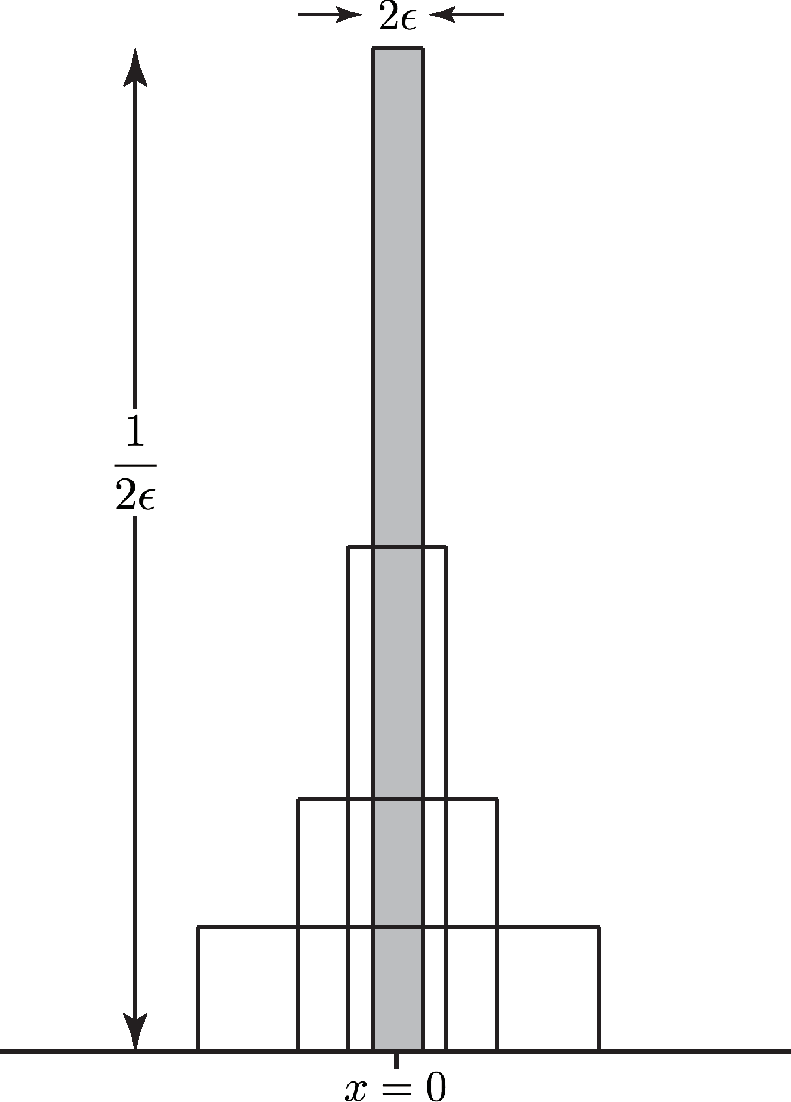
\includegraphics[width=0.5\textwidth]{./Pictures/fig.1.1.pdf}
 \caption{一系列函数递次接近 Dirac delta 函数 $\delta(x)$}
 \label{fg:1.1}
\end{figure}

\exercise{
 应用前面关于 Dirac delta 函数的表述,证明:
 \[a(0) = \int_{-\infty}^\infty \mrm{d}x\,a(x)\delta(x)\]
}

直到现在我们的讨论都与\autoref{sec:1.1.4}中关于$N$维复矢量空间的讨论类似。
确实,完备正交归一函数的理论可以看做普通线性代数的一个推广。
为了方便突显这种相似性,我们引入一种简略表达方式:
\begin{subequations}
 \begin{equation}
     \psi_i(x) \equiv \ket{i} \qquad \psi_i^\ast(x) \equiv \bra{i}
     \label{eq:1.127a}
 \end{equation}
 或更为普遍的:
 \begin{equation}
     a(x) \equiv \ket{a} \qquad a^\ast(x) \equiv \bra{a}
     \label{eq:1.127b}
 \end{equation}
 \label{eq:1.127}
\end{subequations}
以及,两个函数的标量积定义为:
\begin{equation}
 \int \mrm{d}x\,a^\ast(x)b(x) = \olp{a}{b}
 \label{eq:1.128}
\end{equation}
正交归一条件\autoref{eq:1.116}则变为:
\begin{equation}
 \olp{i}{j} = \delta_{ij}
 \label{eq:1.129}
\end{equation}
在这种符号体系下,\autoref{eq:1.118}写作:
\begin{equation}
 \olp{j}{a} = a_j
 \label{eq:1.130}
\end{equation}
因此,\autoref{eq:1.117}变为:
\begin{equation}
 \ket{a} = \sum_i \ket{i}\olp{i}{a}
 \label{eq:1.131}
\end{equation}
需要注意的是,
\autoref{eq:1.129}、\autoref{eq:1.130}和\autoref{eq:1.131}在形式上分别与前一节中的\autoref{eq:1.47}、\autoref{eq:1.48a}和\autoref{eq:1.50a}是完全等同的。

现在我们定义一个算符$\op{O}$,
作用在一个函数$a(x)$上,生成另一个函数$b(x)$:
\begin{subequations}
 \begin{equation}
     \op{O}a(x) = b(x)
     \label{eq:1.132a}
 \end{equation}
 也可以用新引入的符号体系重写为:
 \begin{equation}
     \op{O}\ket{a} = \ket{b}
     \label{eq:1.132b}
 \end{equation}
 \label{eq:1.132}
\end{subequations}
上式与\autoref{eq:1.52}等同。
如果通过需要如下方式计算$b(x)$:
\begin{equation}
 b(x) = \op{O}a(x) = \int\mrm{d}x\,O(x,x^\prime)a(x^\prime)
 \label{eq:1.133}
\end{equation}
则称$\op{O}$为\emph{非定域}算符:
即便我们仅需计算$b(x)$在$x=x_0$处的值,
也需要知道$a(x)$在整个区间上的取值。
非定域算符有时也被称作积分算符。
还需注意,\autoref{eq:1.133}是下式在连续变量情形下的推广:
\begin{equation}
 b_i = \sum_j O_{ij}a_j
 \label{eq:1.134}
\end{equation}
因此,我们可以将$O(x,x^\prime)$看做一个连续矩阵。
如果计算$b(x)$在点$x=x_0$的值时,
只需要知道$a(x)$在$x_0$附近的一个无穷小邻域内的值,
则称$\op{O}$为\emph{定域}算符。
微分算符$\mrm{d}/\mrm{d}x$便是一个定域算符。
如果下面关系成立:
\begin{subequations}
 \begin{equation}
     \op{O}\phi_{\alpha}(x) = \omega_\alpha \phi_\alpha(x)
     \label{eq:1.135a}
 \end{equation}
 或者用 Dirac 符号写为:
 \begin{equation}
     \op{O}\ket{\alpha} = \omega_\alpha\ket{\alpha}
     \label{eq:1.135b}
 \end{equation}
 \label{eq:1.135}
\end{subequations}
与矩阵代数类比,
我们称$\phi_\alpha(x)$为算符$\op{O}$关于本征值$\omega_\alpha$的\emph{本征函数}。
可以选取归一化的函数为本征函数:
\begin{equation}
 \int\mrm{d}x\, \phi_\alpha^\ast(x)\phi_\alpha(x) \equiv \olp{\alpha}{\alpha} = 1
 \label{eq:1.136}
\end{equation}
将\autoref{eq:1.135a}两边乘以$\phi_\alpha^\ast(x)$,
然后对$x$积分,应用\autoref{eq:1.136},
我们得到:
\begin{equation}
 \omega_\alpha = \int \mrm{d}x\,\phi_\alpha^\ast(x)\op{O}\phi_\alpha(x) \equiv \Mele{\alpha}{O}{\alpha}
 \label{eq:1.137}
\end{equation}
此处我们引入了新的符号:
\begin{equation}
 \int\mrm{d}x\,a^\ast(x)\op{O}b(x) = \Mele{a}{O}{b}
 \label{eq:1.138}
\end{equation}
需要注意,我们同样可以在\autoref{eq:1.135b}两边左乘$\bra{a}$,
然后应用归一化条件\eqref{eq:1.136},
得到相同的结果\autoref{eq:1.137}。
此后,我们将把``乘$a^\ast(x)$以然后对$x$积分''简单地表述为``左乘$\bra{a}$''。

与前节相同,
我们同样对 Hermitian算符的本征函数和本征值感兴趣。
Hermitian算符满足如下条件:
\begin{equation}
 \int\mrm{d}x\,a^\ast(x)\op{O}b(x) = \int\mrm{d}x\,b(x)\left(\op{O}a(x)\right)^\ast = \left(\int\mrm{d}x\,b^\ast(x)\op{O}a(x)\right)^\ast
 \label{eq:1.139}
\end{equation}
应用\autoref{eq:1.138}引入的符号,上式可写为:
\begin{equation}
 \Mele{a}{O}{b} = {\Mele{b}{O}{a}}^\ast
 \label{eq:1.140}
\end{equation}
注意上式与\autoref{eq:1.61}具有相同的形式。
Dirac 符号的优美之处在于,它允许我们用完全相同的形式来处理矢量和函数,
以及作用于它们的算符。
比如,\autoref{sec:1.1.6}中关于 Hermitian算符的本征值和本征矢性质的证明,
可以直接应用于 Hermitian算符的本征值和本征函数上。
因此,Hermitian算符的本征函数是正交归一的,
它们对应的本征值为实数。

\exercise{
 为了进一步展示我们所采用的符号体系的自洽性,
 考虑算符$\op{O}$在基组$\left\{\psi_i(x)\right\}$中的矩阵表示:
 已知
 \[\op{O}\psi_i(x) = \sum_j\psi_j(x)O_{ji}\]
 证明
 \[O_{ji} = \int\mrm{d}x\,\psi_j^\ast(x)\op{O}\psi_i(x)\]
 然后应用\autoref{eq:1.127a}和\autoref{eq:1.138},
 用 Dirac 符号重写第一个方程,
 并证明其与\autoref{eq:1.55}等价。
\Next
 考虑如下本征值问题:
 \[\op{O}\phi(x) = \omega\phi(x)\]
 通过将$\phi$在完备基组$\left\{\psi_i(x),\, i = 1, 2, \dots\right\}$ 中展开:
 \[\phi(x) = \sum_i^\infty c_i \psi_i(x)\]
 证明等价于矩阵的本征值问题:
 \[\mbf{O}\mbf{c} = \omega\mbf{c}\]
 此处,$(\mbf{c}_i) = c_i$,$(\mbf{O})_{ij} = \int\mrm{d}x\,psi_i^\ast(x)\psi_j(x)$。
 分别用普通形式和 Dirac 符号完成以上证明。
 需要注意的是,此处$\mbf{O}$是一个无穷矩阵,
 而实际操作中,我们无法处理无穷矩阵。
 为了使问题可操作,
 我们可以选取无穷基组的一个子集$\left\{\psi_i(x),\, i = 1, 2, \dots, N\right\}$。
 如果在这个子空间中重复以上分析,
 我们会得到一个$N\times N$维的本征值问题。
 我们将在\autoref{sec:1.3}中看到,
 此处得到的$N$个本征值是真实本征值的近似。
 重要的是,
 我们需要证明这个截断的本征值问题的最低本征值不低于真实的最低本征值。
\Next

 本小节中我们使用了Dirac符号体系的简化版本,
 这种简化相对于我们的目的来说够用,
 但对矢量和函数之间的密切关系描述过于简单。
 在这个练习中,我们将初步感受一下 Dirac 符号体系的强大之处。
 考虑一个由完备正交归一基矢构成的可数无限集,即:
\[
     \sum_i^\infty \ket{i}\bra{a} = 1
     \tag{1a}\label{eq:e1.17.1a}
\]
\[
     \olp{i}{j} = \delta_{ij}
     \tag{1b}\label{eq:e1.17.1b}
\]
引入连续变量的无限完备基组,
其基组为$\ket{x}$。与\autoref{eq:e1.17.1a}类似:
\[
\int\mrm{d}x\,\ket{x}\bra{x} = 1
\tag{2a}\label{eq:e1.17.2a}
\]
在上式中,我们将\autoref{eq:e1.17.1a}中的加和替换成了积分。
将\autoref{eq:e1.17.2a}两边左乘$\bra{a}$,右乘$\ket{b}$,我们有:
\[
\int\mrm{d}x\, \olp{a}{x}\olp{x}{b} = \olp{a}{b}
\]
与\autoref{eq:1.128}相比,
我们可以认出,
$\olp{a}{x}$即$a^\ast(x)$,$\olp{x}{b}$即$b(x)$。
我们知道$\olp{i}{a}$是$\ket{a}$沿基矢$\ket{i}$的分量。
因此,
我们可以将函数$b(x)$看做是抽象矢量$\ket{b}$在一个具有连续变量的无限多坐标轴的坐标系中沿$x$的分量。
\begin{enumerate}[a.]
 \item 将\autoref{eq:e1.17.2a}两边左乘$\bra{i}$,右乘$\ket{j}$,应用\autoref{eq:e1.17.1b},若有如下关系成立:
 \[
 \psi^\ast_i(x) = \olp{i}{x} \qquad \psi_j(x) = \olp{x}{j}
 \]
 则所得结果与\autoref{eq:1.116}等同。
 \item 将\autoref{eq:e1.17.1a}两边左乘$\bra{x}$,右乘$\ket{x^\prime}$。若有如下关系成立
 \[
 \olp{x}{x^\prime} = \delta(x - x^\prime)
 \tag{2b} \label{eq:e1.17.2b}
 \]
 则所得结果与\autoref{eq:1.120}等同。上式即为\autoref{eq:e1.17.1b}在连续变量情形下的类比。
 \item 将\autoref{eq:e1.17.2a}两边左乘$\bra{x^\prime}$,右乘$\ket{a}$。证明所得方程与\autoref{eq:1.121}等同。
 \item 一个算符$\op{O}$在连续基$\ket{x}$中的矩阵表示为
 \[\Mele{x}{O}{x^\prime} = O(x, x^\prime)\]
 由式$\op{O}\ket{a} = \ket{b}$出发并插入完备性关系,我们有
 \[\op{O}\ket{a} = \op{O}\mbf{1}\ket{a} \int\mrm{d}x\,\op{O}\ket{x}\bra{x}\ket{a} = \ket{b}\]
 将上式左乘$\bra{x^\prime}$,验证结果与\autoref{eq:1.133}等同。
 \item 若有$O_{ij} = \Mele{i}{O}{j}$,验证:
 \[O(x,x^\prime) = \sum_{ij}\psi_i(x)O_{ij}\psi_j^\ast(x)\]
\end{enumerate}
}


\section{变分法}
\label{sec:1.3}
本节讨论近似求解本征值问题的一种重要方法。本征值问题即:
\begin{equation}
 \op{O}\psi(x) =\omega\psi(x)
 \label{eq:1.141}
\end{equation}
我们对此感兴趣是因为不含时的(定态) Schr\"{o}dinger 就是一个本征方程:
\begin{equation}
 \op{H} \ket{\Phi} = \mcr{E} \ket{\Phi}
 \label{eq:1.142}
\end{equation}
其中,$\op{H}$为 Hamiltonian,是一个 Hermitian算符,
$\ket{\Phi}$是波函数,$\op{E}$是体系能量。
除了最简单的体系,无法对Schr\"odinger 方程精确求解,
因此,我们关心如何求得这个本征值问题的近似解。
虽然接下来的内容可以应用于任意的特征值问题,
但是我们将沿用 Schr\"odinger 方程\autoref{eq:1.142}相关的符号和术语。

给定算符$\op{H}$,存在一个 Schr\"odinger 方程的精确解的无限集合,我们用$\alpha$来标记:
\begin{equation}
 \op{H}\ket{\Phi_\alpha} = \op{E}_\alpha\ket{\Phi_\alpha}
 \label{eq:1.143}
\end{equation}
其中
\[
\op{E}_0 \leq \op{E}_1 \leq \op{E}_2 \leq \cdots \leq \op{E}_\alpha \leq \cdots
\]
简便起见,
此处我们假设本征值的集合$\left\{\op{E}_\alpha\right\}$是离散的。
由于$\op{H}$是 Hermitian算符,
其本征值$\mcr{E}_\alpha$是实数,
且其对应的本征函数是正交归一的:
\begin{equation}
 \olp{\Phi_\alpha}{\Phi_\beta} = \delta_{\alpha\beta}
 \label{eq:1.144}
\end{equation}
\autoref{eq:1.143}两边左乘$\bra{\Phi_\beta}$得到:
\begin{equation}
 \Mele{\Phi_\beta}{H}{\Phi_\alpha} = \mcr{E}_\alpha\delta{\alpha\beta}
 \label{eq:1.145}
\end{equation}
此外,我们还假设$\op{H}$的本征函数构成一个完备基,
因此,任意一个与$\left\{\ket{\Phi_\alpha}\right\}$具有相同的边界条件的函数$\vert\tilde{\Phi}\rangle$,都可以写为$\ket{\Phi_\alpha}$的线性组合:
\begin{equation}
 \Ket{\tilde{\Phi}} = \sum_\alpha \mathinner{\Big\vert\Phi_\alpha\Big\rangle} c_\alpha = \sum_\alpha \Big\vert\Phi_\alpha\Big\rangle \Olp{\Phi_\alpha}{\tilde{\Phi}}
 \label{eq:1.146}
\end{equation}
以及
\begin{equation}
 \Bra{\tilde\Phi} = \sum_\alpha c_\alpha^\ast \Big\langle\Phi_\alpha\Big\vert = \sum_\alpha \Olp{\tilde\Phi}{\Phi_\alpha}\Big\langle\Phi_\alpha\Big\vert
 \label{eq:1.147}
\end{equation}

\subsection{变分原理}
\label{sec:1.3.1}
现在我们给出一个重要的定理,即\emph{变分原理},的描述,并给予证明:
对于一个符合恰当边界条件(通常是在无穷远处波函数为零)的归一化的波函数$\ket{\tilde\Phi}$,
其 Hamiltonian 的期望值是精确基态能量的上限。即,若有
\begin{equation}
 \Big\langle\tilde\Phi\Big\vert\tilde\Phi\Big\rangle = 1
 \label{eq:1.148}
\end{equation}
则
\begin{equation}
 \Big\langle\tilde\Phi\Big\vert\op{H}\Big\vert\tilde\Phi\Big\rangle \geq \mcr{E}_0
 \label{eq:1.149}
\end{equation}
此定理的证明比较简单。首先我们考虑
\begin{equation}
 \begin{split}
     \Olp{\tilde\Phi}{\tilde\Phi} &= 1 = \sum_{\alpha\beta}\Big\langle\tilde\Phi\Big\vert\Phi_\alpha\Big\rangle\Big\langle\Phi_\alpha\Big\vert\Phi_\beta\Big\rangle\Big\langle\Phi_\beta\Big\vert\tilde\Phi\Big\rangle = \sum_{\alpha\beta} \Big\langle\tilde\Phi\Big\vert\Phi_\alpha\Big\rangle\delta_{\alpha\beta}\Big\langle\Phi_\beta\Big\vert\tilde\Phi\Big\rangle \\
     &= \sum_\alpha \Big\langle\tilde\Phi\Big\vert\Phi_\alpha\Big\rangle\Big\langle\Phi_\alpha\Big\vert\tilde\Phi\Big\rangle = \sum_\alpha \Big\vert\Big\langle\Phi_\alpha\Big\vert\tilde\Phi\Big\rangle\Big\vert^2
 \end{split}
 \label{eq:1.150}
\end{equation}
其中,我们用到了\autoref{eq:1.144}、\autoref{eq:1.146}和\autoref{eq:1.147}。然后,
\begin{equation}
 \Langle\tilde\Phi\Lvert\op{H}\Lvert\tilde\Phi\Rangle = \sum_{\alpha\beta}\Langle\tilde\Phi\Lvert\Phi_\alpha\Rangle\Langle\Phi_\alpha\Lvert\op{H}\Lvert\Phi_\beta\Rangle\Langle\Phi_\beta\Lvert\tilde\Phi\Rangle = \sum_\alpha \mcr{E}_\alpha \Lvert\Langle\Phi_\alpha\Lvert\tilde\Phi\Rangle\Lvert^2
 \label{eq:1.151}
\end{equation}
上式用到了\autoref{eq:1.145}。最后,由于对于所有$\alpha$有$\mcr{E}_\alpha \geq \mcr{E}_0$,我们得到
\begin{equation}
 \Langle\tilde\Phi\Lvert\op{H}\Lvert\tilde\Phi\Rangle \geq \sum_\alpha \mcr{E}_0\Lvert\Langle\Phi_\alpha\Lvert\tilde\Phi\Rangle\Lvert^2 = \mcr{E}_0\sum_\alpha \Lvert\Langle\Phi_\alpha\Lvert\tilde\Phi\Rangle\Lvert^2 = \mcr{E}_0
 \label{eq:1.152}
\end{equation}
此处我们用到了正交化条件\autoref{eq:1.150}。

关于基态的变分原理告诉我们,
近似波函数的能量总是过高。
因此,可以用期望能量来检测波函数的质量:
能量越低,波函数质量越好。
上述即为变分原理的基础:
我们采用了一个归一化的试探函数$\ket{\tilde\Phi}$,
这个试探函数具有某些参数,
改变这些参数使得期望值$\Mele{\tilde\Phi}{H}{\tilde\Phi}$达到其极小值。
这个极小值就是精确基态能量的变分估值。

\exercise{
 原子单位下,在势场$-\delta(x)$中进行一维运动的电子的 Schr\"odinger 方程为:
 \[
 \left(-\frac{1}{2}\frac{\mrm{d}^2}{\mrm{d}x^2} - \delta(x)\right) \ket{\Phi} = \mcr{E}\ket{\Phi}
 \]
 采用如下试探函数,
 \[\Lvert\tilde\Phi\Rangle = N \mrm{e}^{-\alpha x^2}\]
 应用变分法,验证$-\pi^{-1}$是精确基态能量(-0.5)的一个上限。
 计算中可能会用到如下积分:
 \[
 \int_{-\infty}^{\infty}\mrm{d}x\,x^{2m}\mrm{e}^{-\alpha x^2} = \frac{(2m)!\,\pi^{1/2}}{2^{2m}m!\,\alpha^{m+1/2}}
 \]
\Next
 原子单位下,氢原子的 Schr\"odinger 方程为:
 \[
 \left(-\frac{1}{2}\nabla^2 - \frac{1}{r}\right)\ket{\Phi} = \mcr{E}\ket\Phi
 \]
 应用变分法并采用如下试探函数:
 \[
 \Ket{\tilde{\Phi}} = N \mrm{e}^{-\alpha r^2}
 \]
 验证$-4/3\pi = -0.4244$是精确基态能量(-0.5)的一个上限。
 计算中可能会用到如下公式:
 \[
 \nabla^2f(r) = r^{-2}\frac{\mrm d}{\mrm{d}r}\left(r^2\frac{\mrm d}{\mrm{d}r}\right)f(r)
 \]
 \[
 \int_0^\infty \mrm{d}r\, r^{2m}\mrm{e}^{-\alpha r^2} = \frac{(2m)!\,\pi^{1/2}}{2^{2m+1}m!\,\alpha^{m+1/2}}
 \]
 \[
 \int_0^\infty\mrm{d}r\,r^{2m+1}\mrm{e}^{-\alpha r^2} = \frac{m!}{2\alpha^{m+1}}
 \]
\Next
 将变分原理应用于矩阵本征值问题时用到的列矢量$\mbf{c}$是归一化的($\madj{c}\mbf{c} = 1$),
 由此我们得到$\madj{c}\mbf{Oc}$不低于矩阵$\mbf{O}$的最低本征值的结论。
 对于一个$2\times2$对称矩阵($O_{12}=O_{21}$),
 \[ \mbf{O} = 
 \begin{pmatrix}
     O_{11} & O_{12} \\ O_{21} & O_{22}
 \end{pmatrix}
 \]
 采用归一化的试探矢量
 \[ \mbf{c} = \begin{pmatrix}
     \cos\theta \\ \sin\theta
 \end{pmatrix}
 \]
 计算
 \[\omega(\theta) = \madj{c}\mbf{O}\mbf{c}\]
 并指出使$\omega(\theta)$取极小值的$\theta$,
 即$\theta_0$。
 验证$\omega(\theta_0)$与矩阵$\mbf O$的最低本征值(见\autoref{eq:1.105} 和\autoref{eq:1.106a}相等。
 你对这个结果有什么想法?
}


\subsection{线性变分问题}
\label{sec:1.3.2}
若试探函数$\ket{\tilde\Phi}$包含一系列参数,
则其期望值$\langle\tilde\Phi\vert\op{H}\vert\tilde\Phi\rangle$也取决于这些参数。
通常情况下,
寻找使$\langle\tilde\Phi\vert\op{H}\vert\tilde\Phi\rangle$取极小值的那组参数的值是一个非常复杂的问题,
以至于没有简单的方法来完成。
然而,如果我们只允许试探函数存在线性的变化,即:
\begin{equation}
 \Ket{\tilde\Phi} = \sum_{i=1}^{N} c_i \Lvert\Psi_i\Rangle
 \label{eq:1.153}
\end{equation}
其中,$\left\{\vert\Psi_i\rangle\right\}$是一组\emph{固定}的基函数,
这样我们将问题转变成寻找最优化的系数$\left\{c_i\right\}$将矩阵对角化。

假设我们的基函数是实函数,并满足正交归一条件
\begin{equation}
 \left\langle\Psi_i\middle\vert\Psi_j\right\rangle = \left\langle\Psi_j\middle\vert\Psi_i\right\rangle = \delta_{ij}
 \label{eq:1.154}
\end{equation}
非正交归一的复函数的情形我们将在\autoref{ch:3}中讨论。
Hamiltonian 算符在基组$\left\{\vert\Psi_i\rangle\right\}$中的矩阵表示$\mbf{H}$是一个$N\times N$的矩阵,
其矩阵元为:
\begin{equation}
 \left(\mbf{H}\right)_{ij} = H_{ij} = \Mele{\Psi_i}{H}{\Psi_j}
 \label{eq:1.155}
\end{equation}
由于 Hamiltonian 是 Hermitian,且
基函数为实函数,$\mbf H$为对称矩阵,
即$H_{ij} = H_{ji}$。试探函数满足归一化条件
\begin{equation}
 \Olp{\tilde\Phi}{\tilde\Phi} = \sum_{ij}\Langle\Psi_i\Lvert\Psi_j\Rangle = \sum_i c_i^2 = 1
 \label{eq:1.156}
\end{equation}
其期望值
\begin{equation}
 \Mele{\tilde\Phi}{H}{\tilde\Phi} = \sum_{ij}c_i\Langle\Psi_i\Lvert\op{H}\Lvert\Psi_j\Rangle c_j = \sum_{ij}c_ic_jH_{ij}
 \label{eq:1.157}
\end{equation}
是关于展开系数的函数。

我们的问题是寻找使$\langle\tilde\Phi\vert\op{H}\vert\tilde\Phi\rangle$取极小值的那组参数。
不幸的是,这$N$个参数不是互相独立的,
因此我们不能简单地求解如下方程:
\begin{equation}
 \frac{\partial}{\partial c_k} \Mele{\tilde\Phi}{H}{\tilde\Phi} = 0 \qquad k = 1, 2, \dots, N
 \label{eq:1.158}
\end{equation}
由于试探函数是归一化的,
展开系数之间的关系满足\autoref{eq:1.158},
即只有$N-1$个独立变量。
在约束条件(\autoref{eq:1.156})下将函数~\eqref{eq:1.157}最小化的问题可以用 Lagrange \emph{不定乘子法}来解决:首先构建一个函数

\begin{equation}
 \begin{split}
     \mcr{L}\left(c_1, \dots, c_N, E\right) &= \Mele{\tilde\Phi}{H}{\tilde\Phi} - E\left(\Olp{\tilde\Phi}{\tilde\Phi} - 1\right) \\
     &= \sum_{ij} c_ic_jH_{ij} - E\left(\sum_i c_i^2 -1\right)
 \end{split}
 \label{eq:1.159}
\end{equation}
由于试探函数是归一化的,
实际上我们只在\autoref{eq:1.157}上加了一个零项,
因此函数$\mele{\tilde\Phi}{H}{\tilde\Phi}$ 和$\mcr{L}$在取同一组参数值时同事具有极小值。
如果将$c_1, c_2, \dots, c_{N-1}$选为任意的独立变量,
则$c_N$可以通过归一性条件\autoref{eq:1.156}确定。
这时我们有:
\begin{equation}
 \frac{\partial \mcr{L}}{\partial c_k} = 0 \qquad k = 1, 2, \dots, N-1
 \label{eq:1.160}
\end{equation}
上式并不要求$\partial\mcr{L}/\partial{c_k}$必须为零。
然而,在我们目前的处理过程中还有一个未定乘子$E$,
我们可以选取$E$使得$\partial\mcr{L}/\partial{c_k}$值为零,则有
\begin{equation}
 \frac{\partial \mcr{L}}{\partial c_k} = 0 \qquad k = 1, 2, \dots, N
 \label{eq:1.161}
\end{equation}
因此,
\begin{equation}
 \frac{\partial \mcr{L}}{\partial c_k} = 0 = \sum_j c_j H_{kj} + \sum_i c_i H_{ik} - 2 Ec_k
 \label{eq:1.162}
\end{equation}
又因为 $H_{ij = H_{ji}}$,我们有:
\begin{equation}
 \sum_j H_{ij}c_j - Ec_i = 0
 \label{eq:1.163}
\end{equation}
引入列向量$\mbf c$,其元素为$c_i$,则上式可以写为矩阵式:
\begin{equation}
 \mbf{H}\mbf{c} = E \mbf{c}
 \label{eq:1.164}
\end{equation}
即一个标准的关于矩阵$\mbf{H}$的本征值问题。

由于$\mbf{H}$是对称矩阵,
求解\autoref{eq:1.164}将得到$N$个正交归一的本征矢$\mbf{c}^\alpha$及其对应的本征值$E_\alpha$。
方便起见,我们将本征值按照升序排列,
即$E_0 \leq E_1 \leq \cdots \leq E_{N-1}$。因此,
\begin{equation}
 \mbf{H}\mbf{c}^\alpha = E_\alpha \mbf{c}^\alpha\qquad \alpha = 0, 1, \dots, N-1
 \label{eq:1.165}
\end{equation}
其中,
\begin{equation}
 \left(\mbf{c}^\alpha\right)^\dagger\mbf{c}^\beta = \sum_i c_i^\alpha c_i^\beta = \delta_{\alpha\beta}
 \label{eq:1.166}
\end{equation}
我们还可以引入对角矩阵$\mbf{E}$,
其对角元为前述本征值$E_\alpha$,
即$\left(\mbf{E}\right)_\alpha\beta = E_\alpha\delta_{\alpha\beta}$,
以及由本征矢组成的矩阵$\mbf{C}$,
其中$C_{i\alpha} = c_i^\alpha$,
则\autoref{eq:1.165}包含的$N$个关系可以写作:
\begin{equation}
 \mbf{H}\mbf{C} = \mbf{C}\mbf{E}
 \label{eq:1.167}
\end{equation}

通过上述变换,
我们实际上能够同时求出关于$\ket{\tilde\Phi}$的$N$组而不是一组展开系数:
\begin{equation}
 \Ket{\tilde\Phi} = \sum_{i=1}^N c_i^\alpha \Lvert\Psi_i\Rangle = \sum_{i=1}^N C_{i\alpha}\Lvert\Psi_i\Rangle \qquad \alpha = 0, 1, \dots, N-1
 \label{eq:1.168}
\end{equation}
并且这些本征矢满足正交归一关系:
\begin{equation}
 \Langle\tilde\Phi_\alpha\Lvert\tilde\Phi_\beta\Rangle = \sum_{ij} c_i^\alpha c_j^\beta \Langle\Psi_i\Lvert\Psi_j\Rangle = \sum_{ij}c_i^\alpha c_j^\beta\delta_{ij} = \sum_i c_i^\alpha c_i^\beta = \delta_{\alpha\beta}
 \label{eq:1.169}
\end{equation}
上式推导过程中我们用到了\autoref{eq:1.154}和\autoref{eq:1.166}。
我们还需要发掘一下$E$的物理意义,考虑到:
\begin{equation}
 \begin{split}
     \Langle\tilde\Phi_\beta\Lvert\op{H}\Lvert\tilde\Phi_\alpha\Rangle &= \sum_{ij} c_i^\beta \Langle \Psi_i\Lvert\op{H}\Lvert\Psi_j\Rangle c_j^\alpha \\
     &= \sum_{ij}c_j^\beta H_{ij}c_j^\alpha \\
     &= \left(\mbf{c}^\beta\right)^\dagger\mbf{H}\mbf{c}^\alpha \\
     &= E_\alpha \left(\mbf{c}^\beta\right)^\dagger\mbf{c}^\alpha = E_\alpha \delta_{\alpha\beta}
 \end{split}
 \label{eq:1.170}
\end{equation}
此处我们用到了\autoref{eq:1.165}和\autoref{eq:1.166}。
因此,Hamiltonian 的本征值$E_\alpha$就是 对应于$\ket{\tilde\Phi}$的期望值。
特别的,在基函数$\left\{\vert\Psi_i\rangle\right\}$张开的空间中,
最低本征值$E_0$是$\op{H}$的基态能量的最好近似。
此外,变分原理还保证了
\begin{equation}
 E_0 = \Langle\tilde\Phi_0\Lvert\op{H}\Lvert\tilde\Phi_0\Rangle \geq \mcr{E}_0
 \label{eq:1.171}
\end{equation}
那么其他本征值$E$有什么物理意义呢?
可以证明(见练习~\autoref{ex:1.21})
$E_\alpha \geq \mcr{E}_\alpha,\, \alpha = 1, 2, \dots$,因此,$E_1$是第一激发态能量的上限,以此类推。

\exercise{
          考虑一个归一化的试探函数$\ket{\tilde\Phi^\prime}$,
          其正交于精确的基态波函数,即$\langle \tilde \Phi^\prime \vert \Phi_0 \rangle = 0$
 \begin{enumerate}[a.]
     \item 推广\autoref{sec:1.3.1}中关于变分原理的证明,并验证
     \[\Langle\tilde{\Phi}^\prime\Lvert\op{H}\Lvert\tilde{\Phi}^\prime\Rangle \geq \mcr{E}_1.\]
     \item 考虑如下函数
     \[\Lvert\tilde{\Phi}^\prime\Rangle = x\Lvert\tilde\Phi_0\Rangle + y \Lvert\tilde\Phi_1\Rangle\]
     其中$\ket{\tilde\Phi_\alpha}, \alpha = 0, 1$由\autoref{eq:1.168}给定。
     若该函数归一,证明
     \[\vert x\vert^2 + \vert y \vert^2 = 1.\]
     \item 若选定$x$和$y$使得$\ket{\tilde\Phi^\prime}$归一,
     且满足关系$\olp{\tilde\Phi^\prime}{\Phi_0} = 0$,
     则可由 (a) 得出$\mele{\tilde\Phi^\prime}{H}{\tilde\Phi^\prime} \geq \mcr{E}_1$。
     验证如下关系:
     \[\Mele{\tilde\Phi^\prime}{H}{\tilde\Phi^\prime} = E_1 - \vert x\vert^2 (E_1 - E_0) \]
     由于$E_1 \geq \mcr{E}_0$,我们可以得到结论$E_1 \geq \mcr{E}_1$。推广以上论证,证明$E_\alpha \geq \mcr{E}_\alpha,\, \alpha = 2, 3, \dots .$
 \end{enumerate}
}

总之,线性变分法是在给定一组固定的正交归一函数$\left\{\ket{\Psi_i},\,i=1, 2, \dots, N\right\}$的情况下,
为本征值问题
\begin{equation}
 \op{H}\Ket{\Phi} = \mcr{E}\Ket{\Phi}
 \label{eq:1.172}
\end{equation}
寻找最优近似解的一种方法。
该方法需要在有限基组$\left\{\ket{\Psi_i}\right\}$内构建算符$\op{H}$的矩阵表示,
即$(\mbf{H})_{ij} = \mele{\Psi_i}{H}{\Psi_j}$,
并求解矩阵本征值问题:
\begin{equation}
 \mbf{H}\mbf{c} = E \mbf{c}
 \label{eq:1.173}
\end{equation}
即将$N\times N$矩阵$\mbf H$对角化。

前面我们通过直接对 Hamiltoninan 的期望值求极小值得到上述结论。
然而,还可以通过其他方法来得到\autoref{eq:1.173},
我们将发现这种方法另有助益:
在求解\autoref{eq:1.172}时,假设
\begin{equation}
 \Ket{\Phi} = \sum_{j=1}^N c_j\Ket{\Psi_j}
 \label{eq:1.174}
\end{equation}
将上式带入\autoref{eq:1.172}:
\begin{equation}
 \sum_j c_j \op{H}\Ket{\Psi_j} = \mcr{E} \sum_j c_j \Ket{\Psi_j}
 \label{eq:1.175}
\end{equation}
上式两边左乘$\bra{\Psi_i}$,由于展开\autoref{eq:1.174}为近似式,将$\mcr{E}$替换为$E$,则有:
\[
\sum_j c_j \Mele{\Psi_i}{H}{\Psi_j} = E\sum_j c_j \Olp{\Psi_i}{\Psi_j} = Ec_i
\]
或写为:
\begin{equation}
 \sum_j H_{ij}c_j = E c_i
 \label{eq:1.176}
\end{equation}
上式的矩阵式与\autoref{eq:1.174}等同。
如果使用\emph{完备}的正交归一基组 $\left\{\ket{\Psi_i},
\right. \, i = 1, 2,\allowbreak \dots, N, N+1, \left.\dots \right\}$,
我们则会得到一个与\autoref{eq:1.173}等同,
但其中的$\mbf{H}$为一个无限矩阵。
在这种情况下,矩阵的本征值会与算符$\op{H}$的本征值严格相等。
因此,线性变分法就相当于在由基函数$\left\{\ket{\Psi_i},\,i=1,2,\dots,N\right\}$张开的有限子空间中求解本征值问题\autoref{eq:1.172}。
 
\exercise{
     原子单位下,处于一个指向$z$向的场强为$F$的匀强电场中的氢原子的 Schr\"odinger 方程为:
 \[
 \left(-\frac{1}{2}\nabla^2 - \frac{1}{r} + Fr\cos\theta\right) \Ket{\Phi} = \left(\op{H}_0 + Fr\cos\theta\right)\Ket{\Phi} = \mcr{E}(F)\Ket{\Phi}
 \]
 使用如下试探函数,求$\mcr{E}(F)$的上限。
 \[\Ket{\tilde{\Phi}} = c_1\Lvert 1s\Rangle + c_2 \Lvert 2p_z\Rangle\]
 其中$\ket{1s}$和$\ket{2p_z}$是$\op{H}$的正交归一本征函数,即:
 \[
 \begin{split}
     \Ket{1s} &= \pi^{-1/2}\mrm{e}^{-r} \\
     \Ket{2p_z} &= (32\pi)^{-1/2}r\mrm{e}^{-r/2}\cos\theta
 \end{split}
 \]
 在构建$\op{H}$的矩阵表示时,可以使用如下关系:
 \[
 \op{H}_0 \Ket{1s} = -\frac{1}{2}\Ket{1s},\qquad \op{H}_0 \Ket{2p_z} = -\frac{1}{8}\Ket{2p_z}
 \]
 利用公式$(1+x)^{1/2} \approx 1 + x/2$,将所得结果对$F$进行 Taylor 展开,即:
 \[
 E(F) = E(0) -\frac{1}{2}\alpha F^2 + \cdots
 \]
 其中$\alpha$为体系近似的偶极极化率,验证其值为 2.96。其精确结果为 4.5。
}
 
\addcontentsline{toc}{section}{\protect\numberline{}{扩展阅读}}
 
\begin{description}
 \item{Acton, F. S., \textit{Numerical Methods that Work}, Harper \& Row, New York, 1970.} 该书第13章有关于矩阵本征值问题的各种高效算法的非常好的讨论。
 \item{Cushing, J. T. \textit{Applied Analytical Mathematics for Physical Scientists}, Wiley, New York, 1975.} 该书的前四章对本章中的数学进行了一个严格但易接受的讲述。
 \item{Merzbacher, E., \textit{Quantum Mechanics}, 2nd ed., Wiley, New York, 1970.} 多数研究生用的量子力学教材都完整讲授了 Dirac 符号。该书的第 14 章包含这部分内容的一个导论。
 \item{Press, W. H., Flannery, B. P., Teukolsky, S. A. and Vetterling, W. T. \textit{Numerical Recipes}, Cambridge University Press, Cambridge, 1986.} 在这部科学计算的圣经中,第11章讨论了寻找矩阵本征值和本征矢的多种算法,并提供了 FORTRAN 源码。
\end{description}
%!TEX root = ../main.tex

\chapter{多电子波函数与多电子算符}
\label{chap2}
本章介绍量子化学的基本概念、技巧及必要的记号。
具体有三方面:多电子算符(如哈密顿算符)的结构和多电子波函数的形式(即Slater行列式及其线性组合);
如何求算符在Slater行列式之间的矩阵元;
Hatree-Fock近似的基本思想。
之后的章节就是Hartree-Fock近似和以HF为起点的高级方法,
所以现在学的知识在以后的章节中极有用处。


\autoref{sec2.1}关注电子的问题,即在固定的原子核所产生的场中,电子的行为是怎样的。
这是量子化学的中心问题,也是本书的核心关注点。
如此,首先介绍完整的不含时非相对论Schr\"odinger方程,然后引入Born-Oppenhermer近似。
接下来会对Pauli排斥(反对称原理)作总体的阐述,
这是多电子波函数必须遵守的原理,即在交换任意两电子坐标的操作下,多电子波函数是反对称的。

\autoref{sec2.2}先介绍单电子函数(空间轨道和自旋轨道),
并用单电子函数构建多电子函数(Hartree积和Slater行列式)。
然后用单个Slater行列式来近似体系的精确波函数(属于Hartree-Fock近似)并考察这种近似的特点。
如此之后,我们再介绍一个简单体系:氢分子的极小基(每个原子上一个1s轨道)从头算模型。
这个模型简单却有教学上的优点,本书将频繁使用这个模型。
有些理论乍看非常繁杂,但用这个模型能够揭示出它们的核心特点。
本节最后一部分讨论$N-$电子波函数的多行列式(multi-determinatal)展开。

\autoref{sec2.3}的主要内容是量子化学中的单、双电子算符,以及这些算符在Slater行列式之间的矩阵元,并介绍了如何将这些算符关于自旋轨道的矩阵元转换为关于空间轨道的矩阵元。本节最后介绍了一个技巧以帮助记忆单个Slater行列式所对的应能量表达式。

\autoref{sec2.4}对产生、湮灭算符以及二次量子化形式作了简介。二次量子化是处理多电子体系的一种手段,它天然蕴含Pauli不相容原理,而非直接使用Slater行列式。这种形式广泛出现在多体理论的文献中。不过本书大部分的内容都不要求读者掌握二次量子化,所以跳过这一节也没什么影响。

\autoref{sec2.5}讨论多电子系统中的电子自旋与自旋算符,对限制性和非限制性自旋轨道、自旋匹配组态也作了阐述。自旋匹配组态和由限制性自旋轨道得出的单个Slater行列式不同,前者才是总电子自旋算符的正确的本征函数。本节对单、双、三重的自旋匹配组态,以及非限制性波函数(此函数不是总电子自旋算符的本征函数)作了阐述。

\section{电子的问题}
\label{sec2.1}
本书的主要关注点在于如何近似求解非相对论不含时Schr\"odinger方程
\begin{equation}
\label{2.1}
\scr{H}\ket{\Phi}=\scr{E}\ket{\Phi}
\end{equation}
其中$\scr{H}$是核和电子组成的系统的哈密顿算符,
核的坐标用$\bo{R}_A$记,
电子的用$\bo{r}_i$记. 
\autoref{fig2.1}就是一个分子坐标系的示例。
$i$电子与$A$核之间的距离是$r_{iA}=|\bo{r}_i-\bo{R}_A|$; 
$i$电子和$j$电子的距离是$r_{ij}=|\bo{r}_i-\bo{r}_j|$, 
A核与B核之间的距离为$R_{AB}=|\bo{R}_A-\bo{R}_B|$.
若用原子坐标,
则$N$个电子$M$个核的哈密顿量就是:

\begin{figure}[h]
	\begin{tikzpicture}[scale=2,inner sep=0,arrows=-latex]
		\draw (0,0)--(0,2);
		\draw (0,0)--(-1.2,-1.2);
		\draw (0,0)--(2,0);
		%	\draw[->]       (0,0)--(1,.8);
		%	\draw[->]       (0,0)--(-1,.6);
		\node[shape=circle,draw,minimum size=.4cm] (j) at (2,1) {\bf j};
		\node[shape=circle,draw,minimum size=.4cm] (B) at (-1.2,0.4) {\bf B};
		\node[shape=circle,draw,minimum size=.4cm,] (i) at (.7,1.8) {\bf i};
		\node[shape=circle,draw,minimum size=.4cm] (A) at (-.9,1) {\bf A};
		\draw (0,0)--node[right=13pt]{$\mathbf{r_j}$}(j);
		\draw (0,0)--node[right=5pt]{$\mathbf{r_i}$}(i);
		\draw (0,0)--node[right=2pt,above=7pt]{$\mathbf{R_A}$}(A);
		\draw (0,0)--node[left=3pt,below=2pt]{$\mathbf{R_B}$}(B);
		\draw (B)--node[left=.2cm,]{$\mathbf{R_{AB}}=\mathbf{R_A-R_B}$}(A);
		\draw (A)--node[left=.2cm]{$\mathbf{r_{iA}}=\mathbf{r_i-R_A}$}(i);
		\draw (A)--node[pos=.7,above]{$\mathbf{r_{jA}}=\mathbf{r_j-R_A}$}(j);
		\draw (j)--node[right=.2cm]{$\mathbf{r_{ij}}=\mathbf{r_i-r_j}$}(i);
		\draw[draw=none] (.52,-.5)node{$i,j \equiv \text{电子}$};
		\draw[draw=none] (.4,-.7)node{$A,B\equiv\text{核}$};
	\end{tikzpicture}
	\caption{一个分子中的坐标系:$i,j$=电子;$A,B$=核.}
	\label{fig2.1}
\end{figure}


\begin{equation}
\label{eq:2.2}
\begin{split}
\scr{H}=&-\sum_{i=1}^{N}\frac{1}{2}\nabla_i^2 - \sum_{A=1}^{M}\frac{1}{2M_A}\nabla_A^2 - \sum_{i=1}^{N}\sum_{A=1}^{M}\frac{Z_A}{r_{iA}}\\
+&\sum_{i=1}^{N}\sum_{j>i}^{N}\frac{1}{r_{ij}}+\sum_{A=1}^{M}\sum_{B>A}^M\frac{Z_AZ_B}{R_{AB}}
\end{split}
\end{equation}
这个方程中,
$M_A$是原子核A的质量与电子质量的比值,
$Z_A$是核的原子序号. 
Laplace算符$\nabla_i^2,\nabla_A^2$微分的对象分别是$i$电子的坐标和$A$核的坐标.
\autoref{eq:2.2}中的第一项是全部电子的动能算符,
第二项是核的动能算符,
第三项是核与电子间的Coulomb吸引势能,
第四项和第五项分别是电子间和核之间的排斥势.


\subsection{原子单位}
\label{sec2.1.1}
本书所采用的单位是原子单位. 
为了理解原子单位的由来,
我们先看SI单位下氢原子的Schr\"odinger方程:
\begin{align}
\label{2.3}
\left[-\frac{\hbar^2}{2m_e}\nabla^2-\frac{e^2}{4\pi\varepsilon_0r}\right]\phi=\scr{E}\phi
\end{align}
$ \hbar $是Planck常数除以$ 2\pi $, $ m_e $是电子质量,$ -e $是电子电荷.为将方程变为无量纲形式,进行坐标变换:$x,y,z\to\lambda x,\lambda y,\lambda z$,得到
\begin{equation}
\label{2.4}
\left[-\frac{\hbar^2}{2m_e\lambda^2}\nabla'^2-\frac{e^2}{4\pi\varepsilon_0\lambda r'}\right]\phi'=\scr{E}\phi'
\end{equation}
动能算符核势能算符里面的常数部分可以因子化,
即选定一个$ \lambda $使得
\begin{equation}
\label{2.5}
\frac{\hbar^2}{m_e\lambda^2}=\frac{e^2}{4\pi\epsilon_0\lambda}=\scr{E}_a
\end{equation}
其中$ \scr{E}_a $就是原子坐标下的能量,
叫作\emph{Hartree}.
由\autoref{2.5}可以求得$ \lambda $:
\begin{equation}
\label{2.6}
\lambda=\frac{4\pi\epsilon_0\hbar^2}{m_ee^2}=a_0
\end{equation}
所以$ \lambda $就是Bohr半径$ a_0 $,
在原子单位中是长度单位,
叫作\emph{Bohr}.
最后一点,
由于
\begin{equation}
\scr{E}_a\left[-\frac{1}{2}\nabla'^2-\frac{1}{r'}\right]\phi'=\scr{E}'\phi'	
\end{equation}
如果定义$ \scr{E}'=\scr{E}/\scr{E}_a $,
则可得到无量纲的方程
\begin{equation}
\left(-\frac{1}{2}\nabla'^2-\frac{1}{r'}\right)\phi'=\scr{E}'\phi'
\end{equation}
这就是原子坐标下的Schr\"odinger方程.
该氢原子方程的基态解对应的能量是$-0.5\,\text{原子单位}\equiv -0.5\,\text{Hartrees}$. 
\autoref{t2.1}中列出了原子单位和SI单位之间的转换因子$ X $,
一个量在SI单位中的值$ Q $和原子单位中的值$ Q' $按如下方程联系:
\begin{eqnarray}
\label{2.9}
Q=XQ'
\end{eqnarray}

\begin{table}[h!]
	\centering
	\begin{tabular}{lll}
		\hline
		物理量  & 转换因子$X$                   & $X$的值(SI单位)                                     \\ \hline
		     &  \\
		长度   & $a_0$                     & $ 5.2918\times10^{-11}\,\text{m} $              \\
		质量   & $m_e$                     & $9.1095\times10^{-31}\,\text{kg}$               \\
		电荷   & $e$                       & $1.6022\times 10^{-19}\,\text{C}$               \\
		能量   & $\scr{E}_a$               & $4.6598\times10^{-18}\,\text{J}$                \\
		角动量  & $\hbar$                   & $1.0546\times10^{-34}\,\text{Js}$               \\
		电偶极矩 & $ea_0$                    & $8.4784\times10^{-30}\,\text{Cm}$               \\
		电极化率 & $e^2a_0^2\scr{E}_a^{-1}$  & $1.6488\times10^{-41}\text{C$^2$m$^2$J$^{-1}$}$ \\
		电场强度 & $\scr{E}_ae^{-1}a_0^{-1}$ & $5.1423\times10^{11}\text{Vm$^{-1}$}$           \\
		波函数  & $a_0^{-3/2}$              & $2.5978\times10^{15}\,\text{m$^{-3/2}$}$        \\ \hline
	\end{tabular}
	\caption{SI转换为原子单位}
	\label{t2.1}
\end{table}

下面是一些文献中常见的非SI单位下的物理量的转换因子.
一原子单位长度等于$0.52918$埃($\text{\AA}$).
一原子单位偶极矩(相距$a_0$的两个单位电荷)等于$2.5418$德拜(D),
一原子单位能量等于$27.211$电子伏特(eV), 
627.
51\,
kcal/mole.


从现在起我们开始采用原子单位,
并去掉之前所有量中的撇号.


\subsection{Born-Oppenheimer近似}
\label{sec2.1.2}
Born-Oppenheimer近似在量子化学中占据着核心位置.
这里我们仅对该近似作定性的讨论. Sutcliffe\endnote{
B. T. Sutcliffe, Fundamentals of computational quantum chemistry, in \textit{Computational Techniques in Quantum Chemistry}, G. H. F. Diercksen,  B. T. Sutcliffe, and A. Veillard(Eds), Reidel, Boston, 1975, p. 1.
}
对该近似的定量层面作了清晰的讨论,包括如何推导对该近似的修正等. 
由于原子核远比电子重,所以它们运动得较慢。
因此,很大程度上可将分子中的电子视作在位置固定的核产生的势场中运动。
在这个近似下,\autoref{eq:2.2}中第二项,即核动能项,可以被忽略;式中第三项,即核间排斥势可以视作常量。
任意常数加到算符上产生的效果就是本征值加一常数,而本征函数不变。
\autoref{eq:2.2}中的剩余项称作电子的哈密顿量,或描述在M个点电荷产生的势场中运动的N个电子的哈密顿量,
\begin{equation}
\label{2.10}
\scr{H}_{elec}=-\sum_{i=1}^{N}\frac{1}{2}\nabla_i^2 - \sum_{i=1}^{N}\sum_{A=1}^{M}\frac{Z_A}{r_{iA}} + \sum_{i=1}^{N}\sum_{j>i}^{N}\frac{1}{r_{ij}}
\end{equation}
电子哈密顿量的\sch 方程为
\begin{equation}
\label{2.11}
\scr{H}_{elec\rm}\Phi_{\rm elec}=\scr{E}_{\rm elec}\Phi_{\rm elec}
\end{equation}
其解就是电子波函数,

\begin{equation}
\label{2.12}
\Phi_{\rm elec}=\Phi_{\rm elec}(\{\bo{r}\};\{\bo{R}_A\})
\end{equation}
它描述电子的运动,
并显式依赖于电子坐标,
并以参数的方式依赖于核坐标,
电子能量也参数地依赖于核坐标:
\begin{equation}
\label{2.13}
\scr{E}_{\rm elec}=\scr{E}_{\rm elec}(\{\bo{R}_A\})
\end{equation}

“参数地依赖”是指对每一种不同的核构型,
$\Phi_\mathrm{elec}$(电子坐标的函数)的形式都不一样. 
核坐标并不显示地出现在$\Phi_{\rm elec}$中. 
核固定构型下的总能量需包含核排斥能.
\begin{equation}
\label{2.14}
\scr{E}_{\rm tot}=\scr{E}_{\rm elec}+\sum_{A=1}^{M}\sum_{B>A}^M\frac{Z_AZ_B}{R_{AB}}
\end{equation}
\autoref{2.10}到\autoref{2.14}就构成了所谓的电子问题, 
即本书所关心的.


若电子问题已经得解, 
则接下来可用与电子问题同样的假设来求解核运动. 
因为电子运动远比核快, 
所以一个合理的近似是将\autoref{eq:2.2}中的电子坐标换成坐标的平均值(用电子波函数来取平均). 
由此得到在电子的平均势场中运动的核的\ha,

\begin{equation}
\begin{split}
\scr{H}_{\rm nucl}= &- \sum_{A=1}^{M}\frac{1}{2M_A}\nabla_A^2 + \braket{-\sum_{i=1}^{N}\frac{1}{2}\nabla_i^2 - \sum_{i=1}^{N}\sum_{A=1}^{M}\frac{Z_A}{r_{iA}} + \sum_{i=1}^{N}\sum_{j>i}^{N}\frac{1}{r_{ij}}}\\
& + \sum_{B>A}^M\frac{Z_AZ_B}{R_{AB}}\\
= & - \sum_{A=1}^{M}\frac{1}{2M_A}\nabla_A^2 + \scr{E}_{\rm elec}(\{\bo{R}_A\}) + \sum_{B>A}^M\frac{Z_AZ_B}{R_{AB}}\\
= & - \sum_{A=1}^{M}\frac{1}{2M_A}\nabla_A^2 + \scr{E}_{\rm tot}(\{\bo{R}_A\})
\end{split}
\end{equation}
总能量$ \scr{E}_{\rm tot}(\{\bo{R}_A\}) $是核运动的势能面. 
势能面函数简例如\autoref{f2.2}所示. 
在Born-Oppenheimer近似中, 
有电子问题求解得到势能面, 
核又在势能面上运动. 

\begin{figure}[H]
	\def\FunctionA(#1){180*((0.6/(#1+.5))^(12) -(0.6/(#1+ .5))^(6)) + 60}
	\def\FunctionF(#1){(#1)^3- 3*(#1)}
	\begin{tikzpicture}
	\begin{axis}[
	ticks=none,
	axis y line*=center,
	axis x line*=middle, 
%	axis on top=true,
	xmin=-.45,
	xmax=.9,
	ymin=-50,
	ymax=140,
	height=8.0cm,
	width=8.0cm,
	restrict y to domain=-120:140,
	]
	\addplot [domain=0:1.2, samples=500, mark=none, thick, blue] {\FunctionA(x)};
	\node [left, blue] at (axis cs: 0,120) {$ \scr{E}_{\rm tot}(\{\bo{R}_A\})$};
	\node [above, blue] at (axis cs: .8,0) {$\{\bo{R}_A\}$};
	\end{axis}
	\end{tikzpicture}
	\caption{势能面的图示.}
	\label{f2.2}
\end{figure}
核\sch 方程
\begin{equation}
\scr{H}_{\rm nucl}\Phi_{\rm nucl} = \scr{E}_{\rm nucl}\Phi_{\rm nucl}
\end{equation}的解
\begin{equation}
\Phi_{\rm nucl}=\Phi_{\rm nucl}(\{\bo{R}_A\})
\end{equation}
可以描述分子的振动、转动和平动。
而$\scr{E}$, 
即对\autoref{2.1}中总能量的Born-Oppenheimer近似,
包含着电子能量、振动、转动以及平动能量。
\autoref{2.1}中的精确波函数的Born-Oppenheimer近似就是
\begin{equation}
\Phi(\{\bo{r}_i\};\{\bo{R}_A\}) = \Phi_{\rm elec}(\{\bo{r}\};\{\bo{R}_A\})\Phi_{\rm nucl}(\{\bo{R}_A\})
\end{equation}
从现在起,
我们仅关心由\autoref{2.11}到\autoref{2.14}所代表的电子问题, 
不把注意力放在振动-转动问题上.
以后的表述中将舍弃下标``$\rm elec$", 
 这意味着仅考虑电子哈密顿量和电子波函数. 
在必要和方便的时候, 
我们会区分\autoref{2.13}所带表的电子能量和\autoref{2.14}所代表的总能量 (后者中包括核-核排斥能).


\subsection{反对称/Pauli不相容原理}
\label{sec2.1.3}
方程\autoref{2.10}中的电子哈密顿量只取决于电子的\emph{空间}坐标, 
为了完整描述电子, 
必须引入\emph{自旋}. 
此处采用自旋的非相对论描述, 
即引入两个自旋函数$\alpha(\omega)$和$\beta(\omega)$, 
分别代表自旋朝上和朝下. 
函数变量是$\omega$, 
但该变量并无明显的意义, 
从操作角度而言, 
只需要自旋函数正交完备:
\begin{subequations}
	\begin{align}
\int\dd\omega\alpha^*(\omega)\alpha(\omega)=\int\dd\omega\beta^*(\omega)\beta(\omega)=1\\
\braket{\alpha|\alpha}=\braket{\beta|\beta}=1
	\end{align}
\end{subequations}
\begin{subequations}
	\begin{align}
	\int\dd\omega\alpha^*(\omega)\beta(\omega)=\int\dd\omega\beta^*(\omega)\alpha(\omega)=0\\
	\braket{\alpha|\beta}=\braket{\beta|\alpha}=0
	\end{align}
\end{subequations}
\label{2.20}

其中的积分号仅是形式上的. 
用这种办法引入自旋后, 
电子就由三个空间坐标加一个自旋坐标来描述. 
将这四个坐标写在一起,
用$\bo{x}$来表示:
 \begin{equation}
 \label{2.21}
 \bo{x}=\{\bo{r},\omega\}
 \end{equation}

 随之, $N$电子波函数的变量就是$ \bo{x_1,x_2,\cdots ,x_N} $, 即写作$\Phi(\bo{x_1,x_2,\cdots ,x_N})$.
 
由于哈密顿算符中并无自旋,
仅仅在波函数中强加自旋无法产生任何后果。
但若对波函数加上一个额外的约束,就能得到一个完善的理论: 
\emph{
	多电子波函数在交换任意两个电子坐标的操作下,必须是反对称的:
}
\begin{equation}
\label{2.22}
\Phi(\bo{x_1,\cdots,x_i,\cdots,x_j,\cdots ,x_N})=-\Phi(\bo{x_1,\cdots,x_j,\cdots,x_i,\cdots ,x_N})
\end{equation}

这个额外的要求有时叫作\emph{反对称原理}, 
它是我们熟悉的Pauli不相容原理最常见的一种表述. 
这个原理是量子力学的基本假设之一. 
波函数不仅要满足\sch 方程, 
也要满足反对称要求, 即\autoref{2.20}. 
以后我们就会明白, 反对称性可以用Slater行列式来保证.
 
\section{轨道, Slater行列式,基函数}
\label{sec2.2}
本节来学习如何写出用来描述多电子系统波函数,以及各种命名和约定俗成的习惯。
这里我们仅考虑用单Slater行列式或Slater行列式的线性组合来刻画多电子波函数。
有时量子化学研究者也用其他特殊的函数形式来刻画一些小体系的波函数,
但大部分情况下还是用Slater行列式。
学习多电子波函数之前, 我们先来讨论单电子的波函数.
 
 \subsection{自旋轨道与空间轨道}
 \label{sec2.2.1}
 \emph{轨道}就是单粒子(这里是一个电子)的波函数. 我们关心分子中的电子, 所以将分子中电子的波函数叫作\emph{分子轨道}. 而所谓\emph{空间轨道}$\psi_i(\bo{r})$, 则是位置矢量 $\bo{r}$的函数, 用来描述电子的空间分布: $|\psi_i(\bo{r})|^2\dd \bo{r}$即在包含$\bo{r}$的体积微元$\dd\bo{r}$中找到电子的概率. 常认为空间分子轨道构成一组正交基
 \begin{equation}
 \int\dd\bo{r}\psi_i^*(\bo{r})\psi_j(\bo{r})=\delta_{ij}
 \end{equation}
 若空间轨道集合$\{\psi_i \}$是完备的, 则用它可以精确地展开任意函数:
 \begin{equation}
 f(\bo{r})=\sum_{i=1}^{\infty}a_i\psi_i(\bo{r})
 \end{equation}
其中$a_i$是常系数. 
绝大多数情况, 
这个集合想要完备则其元素必须无限多, 
但实际运算时不可能用到完备集, 
而是只用其中有限的一部分$\{\psi_i|i=1,2,\cdots,K\}$(共$K$个轨道). 
这个有限集合只是完备集中特定的一部分, 
使用这$K$个轨道来展开, 
我们就认为这种展开在这个子空间中是``精确"的了.


为完整描述一个电子, 
需要指定电子自旋. 
描述电子自旋的完备集包括两个相互正交的函数$\alpha(\omega),\,\beta(\omega)$, 
代表自旋朝上($\uparrow$)和自旋朝下($\downarrow$). 
描述自旋和空间两部分的波函数叫作\emph{自旋轨道},
$\chi(\bo{x})$,
其中$\bo{x}$代表自旋坐标与空间坐标(\autoref{2.21}). 
每个空间轨道都可以构造两个自旋轨道--一个对应自旋向上,
一个对应向下, 
只需要将空间轨道乘以$\alpha$或$\beta$即可, 
如下式:
\begin{equation}
	\chi(\bo{x})=
	\begin{cases}
	\psi(\bo{r})\alpha(\omega)\\
	\text{or}\\
	\psi(\bo{r})\beta(\omega)
	\end{cases}
\end{equation}
给定一由$K$个空间轨道组成的集合$\{\psi_i|i=1,2,\cdots,K \}$, 
就可以构造$2K$个自旋轨道$\{\chi_i|i=1,2,\cdots, 2K\}$:
\begin{equation}
\begin{rcases}
	\chi_{2i-1}(\bo{x})=\psi_i(\bo{r})\alpha(\omega)\\
	\chi_{2i}(\bo{x})=\psi_i(\bo{r})\beta(\omega)
\end{rcases}
i=1,2,\cdots,K
\end{equation}
若空间轨道相互正交, 
则自旋轨道也相互正交:
\begin{equation}
\int\dd\bo{x}\chi_i^*(\bo{x})\chi_j(\bo{x})=\braket{\chi_i|\chi_j}=\delta_{ij}
\end{equation}
\begin{xercise}
给定一组$K$个正交空间轨道\{$\psi_i^\alpha(\bo{r})$\}与另一组$K$个正交空间轨道$\{\psi_i^\beta(\bo{r})\}$, 
但第一组和第二组之间不正交, 
即
\[
\int\dd\bo{r}\psi_i^{\alpha*}(\bo{r})\psi_j^\beta(\bo{r})=S_{ij}
\]
其中$\bo{S}$是重叠矩阵. 
请证明, 
由第一组轨道乘以$\alpha$自旋函数生成的自旋轨道, 
由第二组轨道乘以$\beta$自旋函数生成的自旋轨道, 
总共$2K$个轨道$\{\chi_i \}$:
\begin{equation*}
\begin{rcases}
\chi_{2i-1}(\bo{x})=\psi_i^\alpha(\bo{r})\alpha(\omega)\\
\chi_{2i}(\bo{x})=\psi_i^\beta(\bo{r})\beta(\omega)
\end{rcases}
i=1,2,\cdots,K
\end{equation*}
它们之间相互正交.

\end{xercise}
\subsection{Hartree积}
 \label{sec2.2.2}
学习过用自旋轨道描述单电子之后, 
现在来考虑电子集合的波函数, 
即 $N$电子波函数. 
在考察相互作用系统的精确波函数之前, 
先来看一个较简单的情况: 无相互作用电子的集合, 
其哈密顿量形式如下:
\begin{equation}
\label{2.28}
\scr{H}=\sum_{i=1}^{N}h(i)
\end{equation}
其中$h(i)$是描述电子i的动能和势能的算符. 
若忽略电子间排斥, 
则电子哈密顿就具有这种形式. 
除此之外, 
我们也能将$h(i)$视作有效单电子哈密顿量, 
即以平均的方式将电子间的排斥纳入.


算符$h(i)$有它自己的一组本征函数, 
我们将其视作一组自旋轨道$\{\chi_j\}$:
\begin{equation}
\label{2.29}
h(i)\chi_j(\bo{x}_i)=\epsilon_j\chi_j(\bo{x}_i)
\end{equation}
现在的问题是, 
知道了$h(i)$的本征函数, 
那$\scr{H}$的本征函数是什么? 由于$\scr{H}$是单电子哈密顿量之和, 
如果将每个电子的自旋轨道乘在一起:
\begin{equation}
\label{2.30}
\Psi^{\rm HP}(\bo{x_1,x_2,\cdots,x_N})=\chi_i(\bo{x_1})\chi_j(\bo{x_2})\cdots\chi_k(\bo{x_N})
\end{equation}
它就是$\scr{H}$的一个本征函数:
\begin{equation}
\label{2.31}
\scr{H}\Psi^{\rm HP}=E\Psi^{\rm HP}
\end{equation}
本征值是$E$, 
$E$是$\Psi^{\rm HP}$中每个自旋轨道的能量之和:
\begin{equation}
\label{2.32}
E=\epsilon_i + \epsilon_j + \cdots + \epsilon_k
\end{equation} 
我们把这样的多电子波函数叫作\emph{Hartree积}, 
其中电子1用$\chi_i$描述. 
电子2用$\chi_j$描述, 
如此.


\exercise{证明\autoref{2.30}中的Hartree积是$\scr{H}=\sum_{i=1}^Nh(i)$的本征函数, 本征值是\autoref{2.32}.}

Hartree积是独立电子波函数(或者叫无相关波函数, uncorrelated), 因为
\begin{equation*}
|\Psi^{\rm HP}(\bo{x_1,\cdots,x_N})|^2\dd\bo{x_1}\cdots\dd\bo{x_N}
\end{equation*}

即在体积微元$\dd\bo{x_1}$中找到电子1的概率, 
同时在$\dd\bo{x_2}$中找到电子2的概率, 
等等, 
就等于(按照\autoref{2.30}的定义):
\begin{equation*}
|\chi_i(\bo{x_1})|^2\dd\bo{x_1}|\chi_j(\bo{x_2})|^2\dd\bo{x_2}\cdots|\chi_k(\bo{x_N})|^2\dd\bo{x_N}
\end{equation*}

即电子1在$\dd\bo{x_1}$的概率乘以电子2在$\dd\bo{x_2}$的概率等等等等. 
这种情况与扑克牌很类似: 52张牌中找到红心A的概率(1/52)等于红心的概率(1/4)乘以A的概率(1/13), 
因为红心的概率和A的概率是不相关的(独立的). 
Hartree积就意味着在空间中一点找到电子1的概率与找到电子2的概率是独立的. 
但实际上, 
电子1和2每时每刻都在通过Colomb(库伦)作用相互排斥, 
电子1会尽可能避开电子2所在的区域, 
所以两个电子之间明显是相互关联着的. 
举个相关概率的例子: 2个热土豆和2个冷苹果放在桶内, 
随机取一个处来, 
取到热的东西的概率是1/2, 
取到土豆的概率是1/2, 
但取到热土豆的概率是1/2, 
不等于前两者之积, 
原因是``热"属性和``土豆"属性完全是相互关联着的.


即使假设电子相互独立, 
哈密顿量取\autoref{2.28}的形式, 
Hartree积仍有天然的缺陷: 它将电子1放在$\chi_i$轨道上, 
电子2放在$\chi_j$轨道上, 
把它们很明显地区分开来, 
而没有考虑到电子之间不可分辨. 
反对称原理不区分全同的电子, 
它要求电子波函数在交换任意两个电子坐标的操作下必须反对称(改变正负).

\subsection{Slater行列式}
 \label{sec2.2.3}
Hartree积不满足反对称原理,
但我们可以用如下方式得到反对称的波函数。
考虑一个两电子系统,
自旋轨道分别是$\chi_i$和$\chi_j$,
若将电子1放在$\chi_i$上、电子2放在$\chi_j$上,则有
\begin{equation}
\begin{subequations}
\Psi^{\rm HP}_{1\,2}(\bo{x_1,x_2})=\chi_i(\bo{x_1})\chi_j(\bo{x_2})\tag{2.33a}
\end{subequations}
\end{equation}
\label{2.33a}
另一方面, 
若置电子1于$\chi_j$轨道, 
电子2于$\chi_i$轨道, 
则有
\begin{equation*}
\addtocounter{equation}{-1}
\Psi^{\rm HP}_{1\,2}(\bo{x_1,x_2})=\chi_i(\bo{x_2})\chi_j(\bo{x_1})\tag{2.33b}
\end{equation*}
\label{2.33b}
这两种Hartree积都明显地区分电子, 
但是如果将这两种Hartree积线性组合在一起, 
则可以得到满足反对称原理的波函数:
\begin{equation}
\label{2.34}
\Psi(\bo{x_1,x_2})=2^{-1/2}(\chi_i(\bo{x_1})\chi_j(\bo{x_2})-\chi_i(\bo{x_2})\chi_j(\bo{x_1}))
\end{equation}
$2^{-1/2}$是归一化因子. 式中的符号保证了$\Psi(\bo{x_1,x_2})$在交换电子1和2的坐标时是反对称的:
\begin{equation}
\Psi(\bo{x_1,x_2})=-\Psi(\bo{x_2,x_1})
\end{equation}
从\autoref{2.34}出发, 
很明显, 
当两个电子同时占据相同的自旋轨道时(即$i=j$), 
电子波函数为0. 
由此, 
从反对称原理能立马导出Pauli不相容原理: 不能有超过一个电子占据一个自旋轨道.


\exercise{证明\autoref{2.34}中的波函数$\Psi(\bo{x_1,x_2})$是归一化的
\Next
若$\chi_i$和$\chi_j$是某单电子算符$h$(见\autoref{2.29})的本征函数, 
对应本征值为$\epsilon_i,\epsilon_j$. 
证明, 
方程\autoref{2.33a} \autoref{2.33b}中的Hartree积和\autoref{2.34}中的反对称波函数都是独立电子哈密顿量$\scr{H}=h(1)+h(2)$(见\autoref{2.28})的本征函数, 
本征值是$\epsilon=\epsilon_i+\epsilon_j$}.


反对称波函数(\autoref{2.34})可以写成行列式形式:
\begin{equation}
\Psi(\bo{x_1,x_2})=\frac{1}{2^{1/2}}
\begin{vmatrix}
\chi_i(\bo{x_1})&\chi_j(\bo{x_1})\\
\chi_i(\bo{x_2})&\chi_j(\bo{x_2})
\end{vmatrix}
\end{equation}
这式子叫作\emph{Slater行列式}.
对于$N$电子系统, 
上式推广为
\begin{equation}
\Psi(\bo{x_1,x_2,\cdots,x_N})=\frac{1}{(N!)^{1/2}}
\begin{vmatrix}
\chi_i(\bo{x_1})&\chi_j(\bo{x_1})&\cdots&\chi_k(\bo{x_1})\\
\chi_i(\bo{x_2})&\chi_j(\bo{x_2})&\cdots&\chi_k(\bo{x_2})\\
\vdots			&\vdots			& \,&\vdots\\
\chi_i(\bo{x_N})&\chi_j(\bo{x_N})&\cdots&\chi_k(\bo{x_N})
\end{vmatrix}
\end{equation}

$(N!)^{-1/2}$是归一化因子. 
这个Slater行列式代表N个电子占据N个自旋轨道$(\chi_i,\chi_j,\cdots,\chi_k)$, 
而且没有规定哪个电子在哪个轨道中. 
注意Slater行列式中, 行表示电子: 第一行$(\bo{x_1})$,第一行$(\bo{x_2})$等等; 
列表示自旋轨道: 第一列$(\chi_i)$,第一列$(\chi_j)$等等. 
交换两个电子的坐标相当于交换行列式中的两行,行列式交换两行则变号。
因此Slater行列式满足反对称原理。
若两个电子同时占据一个自旋轨道就意味着行列式有两列是一样的,
此时行列式为$0$,
所以不能够有多于一个电子占据一个自旋轨道(Pauli不相容原理)。
为简便计, 引入归一化的Slater行列式的简写符号: 隐去归一化因子, 仅写出行列式的对角项:
\begin{equation}
\label{2.38}
\Psi(\bo{x_1,x_2,\cdots,x_N})=\ket{\chi_i(\bo{x_1})\chi_j(\bo{x_2})\cdots\chi_k(\bo{x_N})}
\end{equation}

若我们默认电子坐标记号的顺序是$\bo{x_1,x_2,\cdots,x_N}$, 
那么\autoref{2.38}可以继续简写为
\begin{equation}
\Psi(\bo{x_1,x_2,\cdots,x_N})=\ket{\chi_i\chi_j\cdots\chi_k}
\end{equation}

由于交换行列式中的两行要改变符号, 
所以上式中自旋轨道的顺序很重要. 
在这种简计符号中, 
Slater行列式的反对称性表现在:
\begin{equation}
\ket{\cdots\chi_m\cdots\chi_n\cdots}=-\ket{\cdots\chi_n\cdots\chi_m\cdots}
\end{equation}

一个Slater行列式完全由构成它的自旋轨道(即被占据的自旋轨道)决定。由正交归一的自旋轨道构成的Slater行列式是归一化的。由不同的正交归一的自旋轨道构成的N电子Slater行列式相互正交。

\exercise{考虑如下Slater行列式:
\begin{align*}
\ket{K}=\ket{\chi_i\chi_j}\\
\ket{L}=\ket{\chi_k\chi_l}
\end{align*}
请证明\begin{equation*}
\braket{K|L}=\delta_{ik}\delta_{jl}-\delta_{il}\delta_{jk}
\end{equation*}
注意, 
上式两个Slater行列式之间的重叠积分只有如下情况不是0: 1)$k=i$且$l=j$, 
此时$\ket{K}=\ket{L}$, 
重叠积分为1. 
2)$k=j$且$l=i$, 
此时$\ket{L}=\ket{\chi_j\chi_i}=-\ket{K}$, 
重叠积分为-1.

}

到此, 
我们已经知道Hartree积是独立电子波函数, 
因为同时在$\dd\bo{x_1}$(在$\bo{x_1}$附近)找到电子1的概率和在$\dd\bo{x_2}$内(在$\bo{x_2}$附近)找到电子2的概率是二者的乘积. 
将Hartree积反对称化后, 
可以得到Slater行列式, 
这样就引入了\emph{交换}作用, 
交换作用得名于这个规定(要求): $|\Psi|^2$在交换两个电子的空间及自旋坐标的操作下,
保持不变。 
须指出, 
Slater行列式中包括了\emph{交换关联}, 
\emph{交换关联}的意思是,
自旋平行的两个电子的运动是相互关联的. 
由于在Slate行列式中,
自旋反平行的电子之间依然缺失关联作用,
我们也习惯把Slater行列式叫作无相关波函数.


为了理解交换关联的来源, 
我们来看,
把Hartree积反对称化之后, 
电子密度受什么影响. 
考虑双电子Slater行列式, 
自旋轨道分别为$\chi_1,\chi_2$(即这两个轨道被占据):
\begin{equation}
\Psi(\bo{x_1,x_2})=\ket{\chi_1(\bo{x_1})\chi_2(\bo{x_2})}
\end{equation}
若两电子自旋相反, 
而且占据不同的空间轨道:
\begin{align}
\chi_1(\bo{x_1})=\psi_1(\bo{r_1})\alpha(\omega_1)\\
\chi_2(\bo{x_2})=\psi_2(\bo{r_2})\beta(\omega_2)
\end{align}
那么由此可以得到Slater行列式, 
将其展开就得到:
\begin{equation}
\label{2.44}
|\Psi|^2\dd\bo{x_1}\dd\bo{x_2}=\frac{1}{2}|\psi_1(\bo{r_1})\alpha(\omega_1)\psi_2(\bo{r_2})\beta(\omega_2)-\psi_1(\bo{r_2})\alpha(\omega_2)\psi_2(\bo{r_1})\beta(\omega_1)|^2\dd\bo{x_1}\dd\bo{x_2}
\end{equation}
这就是同时在$\dd\bo{x_1}$找到电子1和在$\dd\bo{x_2}$找到电子2的概率. 
记$P(\bo{r_1,r_2})\dd\bo{r_1}\dd\bo{r_2}$为在$\dd\bo{r_1}$(在$\bo{r_1}$附近)找到电子1和在$\dd\bo{r_2}$(在$\bo{r_2}$附近)找到电子2的概率, 
如图2.
3所示. 
这个概率可以如此得到: 将\autoref{2.44}对两电子的自旋坐标积分:
\begin{align}
\label{2.45}
P(\mathbf{r}_1,\mathbf{r}_2)\dd\bo{r_1}\dd\bo{r_2}&=\int\dd\omega_1\dd\omega_2|\Psi|^2\db{r_1}\db{r_2}\notag\\
&=\frac{1}{2}\left[|\psi_1(\bo{r_1})|^2|\psi_2(\bo{r_2})|^2+|\psi_1(\bo{r_2})|^2|\psi_2(\bo{r_1})|^2\right]\db{r_1}\db{r_2}
\end{align}

\begin{figure}[h]
	\centering
	\begin{tikzpicture}[scale=2]
	\draw[->,thick] (0,0)--(0,2);
    \draw[->,thick]                (0,0)--(-1.2,-1.2);
    \draw[->]                (0,0)--(1,1);
    \draw[->]                (0,0)--(-1,1);
    \draw[->,thick]                (0,0)--(2,0);
	\node[below right] at (0.5,0.5) {$\bo{r_2}$};
	\node[below left]  at (-0.5,0.5) {$\bo{r_1}$};
	% 1st box denoted dr_1
	\draw[thick] (-1,1)--(-1.1,1)
	             (-1,1)--(-0.95,1.05)
	             (-1.1,1)--(-1.1,1.1)
	             (-1.1,1.1)--(-1.05,1.15)
	             (-1.05,1.15)--(-0.95,1.15)
	             (-0.95,1.15)--(-0.95,1.05)
	             (-1.1,1.1)--(-1,1.1)
	             (-1,1.1)--(-1,1);
	\draw (-1,1.1)--(-0.95,1.15);
	% 2nd box denoted dr_2
	\draw[thick] (1,1)--(1.1,1)
	             (1,1)--(0.95,1.05)
	             (1.1,1)--(1.1,1.1)
	             (1.1,1.1)--(1.05,1.15)
	             (1.05,1.15)--(0.95,1.15)
	             (0.95,1.15)--(0.95,1.05)
	             (1.1,1.1)--(1,1.1)
	             (1,1.1)--(1,1);
	\draw (1,1.1)--(0.95,1.15);
	\node[above] at (-1.05, 1.15) {$\db{r_1}$} ;
	\node[above] at (1.05, 1.15) {$\db{r_2}$} ;
	\node[below] at (1,-0.5) {$P(\bo{r_1,r_2})\db{r_1}\db{r_2}$};
	\end{tikzpicture}
	\caption{电子1在$\db{r_1}$电子2在$\db{r_2}$的概率}
\end{figure}

如果我们\emph{预设}电子1占据$\psi_1$, 
电子2占据$\psi_2$, 
那么\autoref{2.45}中第一项是在$\db{r_1}$($\db{r_1}$附近)找到电子1的概率乘以在$\db{r_2}$($\db{r_2}$附近)找到电子2的概率. 
第二项代表电子1占据$\psi_2$以及电子2占据$\psi_1$. 
由于电子不可分辨, 
正确的概率应当是二者的平均, 
这正是该式所表达的. 
因此, 
两个电子的运动之间没有相关. 
若$\psi_1=\psi_2$, 
这将更加明显:
\begin{equation}
P(\bo{r_1,r_2})=|\psi_1(\bo{r_1})|^2|\psi_1(\bo{r_2})|^2
\end{equation}
注意$P(\bo{r_1,r_2})$永远不等于0, 
所以总有有限的概率找到两个自旋相反的电子在同一空间点.


若两电子自旋相同(比如$\beta$), 
那么
\begin{align}
\chi_1(\bo{x_1})=\psi_1(\bo{r_1})\beta(\omega_1)\\
\chi_2(\bo{x_2})=\psi_2(\bo{r_2})\beta(\omega_2)
\end{align}
仿照上面的步骤有
\begin{align}
P(\bo{r_1,r_2})&=\frac{1}{2}\big\{|\psi_1(\bo{r_1})|^2|\psi_2(\bo{r_2})|^2+|\psi_1(\bo{r_2})|^2|\psi_2(\bo{r_1})|^2\notag\\
&\quad - \left[\psi^*_1(\bo{r_1})\psi_2(\bo{r_1}) \psi^*_2(\bo{r_2})\psi_1(\bo{r_2}) + \psi_1(\bo{r_1})\psi_2^*(\bo{r_1})\psi_2(\bo{r_2})\psi_1^*(\bo{r_2})\right]\big\}
\end{align}
此式中多出一个交叉项, 
因此概率是相关的. 
这就是同自旋电子之间的交换相关作用. 
注意$P(\bo{r_1,r_1})=1$, 
所以两个同自旋电子处在同一点的概率为0. 
我们称电子周围有\emph{费米穴}. 
总之, 
在单Slater行列式语言中, 
同自旋电子之间的运动是相关的, 
自旋相反的电子是不相关的.


\subsection{Hatree-Fock近似}
 \label{sec2.2.4}
自量子力学诞生以来, 
量子化学的主要任务就是求出并解释\sch 方程的近似解. 
除了特别简单的体系如$\text{H}^+_2$外, 
量子化学所面对的都是多电子问题. 
解决这种问题的核心思想, 
当然也是本书的核心, 
就是Hartree-Fock近似. 
这个近似在展开现代量子化学的内容时非常重要. 
此外, 
很多更精确的方法的第一步就是HF近似. 
到了学一点HF近似的基本思想的时候了! 到了第三章对此会有更具体的阐述.


描述$N$电子系统基态最简单的反对称波函数, 
是单Slater行列式:
\begin{equation}
\label{2.50}
\ket{\Psi_0}=\ket{\chi_1\chi_2\cdots\chi_N}
\end{equation}
变分原理称, 
如上形式的波函数中, 
最优的波函数应该给出最低的能量:
\begin{equation}
E_0=\braket{\Psi_0|\scr{H}|\Psi_0}
\end{equation}
$\scr{H}$是全电子哈密顿量. 
变分中可变动的地方就是\autoref{2.50}中的自旋轨道. 
选择不同的自旋轨道, 
求出最小能量, 
由此可以导出一个方程: Hartree-Fock方程, 
它决定了最优的自旋轨道. 
第三章将会证明Hartree-Fock方程是如下的本征值方程:
\begin{equation}
f(i)\chi(\bo{x}_i)=\epsilon\chi(\bo{x}_i)
\label{2.52}
\end{equation}
$f(i)$是一有效单电子算符,叫Fock算符, 其形式为:
\begin{equation}
\label{2.53}
f(i)=-\frac{1}{2}\nabla_i^2 - \sum_{A=1}^M\frac{Z_A}{r_{iA}} + v^{\rm HF}(i)
\end{equation}
$v^{\rm HF}(i)$是i电子感受到其他电子对其造成的平均势, 其定义会在第三章给出. Hartree-Fock近似的精髓在于将复杂的多电子问题转换为单电子问题, 而单电子问题是以平均的方式处理电子之间的排斥.

Hartree-Fock势$v^{\rm HF}(i)$, 或者叫作i电子感受到的场, 由其他电子的自旋轨道决定(即Fock算符依赖于它的本征函数).  因此Hartree-Fock方程\autoref{2.52}是非线性方程, 只能迭代求解. 求解HF方程的办法叫作自洽场(self-consistent-field, SCF)方法.

SCF的基本想法比较简单. 首先对自旋轨道作一个初始猜测, 此时就可以算出每个电子感受到的平均场$v^{\rm HF}$, 然后就可以利用这个有效势解方程\autoref{2.52}, 得到一组新的自旋轨道. 再用新自旋轨道得到新的平均场, 重复这个步骤直到方程自洽(即直到有效场不再变化, 自旋轨道与Fock算符的本征函数一致).

Hartree-Fock本征值问题\autoref{2.52}的解是一组正交的Hartree-Fock自旋轨道$\{\chi_k\}$和一组对应的本征值$\{\varepsilon_k\}$. N个有最低能量的自旋轨道称为\emph{被占}自旋轨道或\emph{穴}自旋轨道. 由这N个轨道生成的Slater行列式就是Hartree-Fock基态波函数, 也即Hartree-Fock单Slater行列式框架下体系波函数的最优变分近似. 我们暂且将占据轨道的指标记为$a,b,c\cdots$(即$\chi_a,\chi_b,\chi_c,\cdots$). 余下的轨道就是\emph{虚自旋轨道}, 或者叫\emph{未占据自旋轨道、粒子自旋轨道(particle)}. 暂将虚自旋轨道指标记为$r,s,t\cdots$($\chi_r,\chi_s,\chi_t,\cdots$).

\usetikzlibrary{decorations.pathreplacing}
\usetikzlibrary{decorations.pathmorphing}
\begin{figure}[h]
	\centering
	\begin{tikzpicture}[scale=2]
% virtual orbitals
	\node[text width = 1em] at (0.3, 1.15) {\bf 虚自旋轨道};
	\draw[decorate,decoration={brace, amplitude=0.4cm}, line width=0.1cm] (0.8,0.3) -- (0.8,2); 
	\draw[ultra thick] (1, 2)--(3,2) node[right]{$\chi_{2K}$};
	\fill[black] (2,1.55) circle (0.05cm);
	\fill[black] (2,1.70) circle (0.05cm);
	\fill[black] (2,1.85) circle (0.05cm);
	\draw[ultra thick] (1,1.40)--(3,1.40) node[right]{$\chi_s$};
	\draw[ultra thick] (1,1)--(3,1) node[right]{$\chi_r$};
	\fill[black] (2,0.75) circle (0.05cm);
	\fill[black] (2,0.6) circle (0.05cm);
	\fill[black] (2,0.45) circle (0.05cm);
	\draw[ultra thick] (1, 0.3)--(3,0.3)node[right]{$\chi_{N+1}$};
% the divisioin line
	\draw[decorate,decoration={coil,aspect=0,segment length=0.5cm}, line width = 0.15cm] (0, -0.2)--(4,-0.2);
%occupied oribtals
	\draw[decorate,decoration={brace, amplitude=0.4cm}, line width=0.1cm] (0.8, -2.85) -- (0.8, -0.7);
	\node[text width = 1em] at (0.3,-1.775){\bf 占据自旋轨道};
	\draw[thick] (1, -0.7)--(3, -0.7) node[right]{$\chi_N$};
	\node at (2,-0.75){\Huge*};
	\fill[black] (2,-0.85) circle (0.05cm);
	\fill[black] (2,-1) circle (0.05cm);
	\fill[black] (2,-1.15) circle (0.05cm);
	\draw[thick] (1, -1.35)--(3, -1.35) node[right]{$\chi_a$};
	\node at (2,-1.4){\Huge*};
	\draw[thick] (1, -1.75)--(3, -1.75) node[right]{$\chi_b$};
	\node at (2,-1.8){\Huge*};
	\fill[black] (2,-1.9) circle (0.05cm);
	\fill[black] (2,-2.05) circle (0.05cm);
	\fill[black] (2,-2.2) circle (0.05cm);
	\draw[thick] (1, -2.4)--(3, -2.4) node[right]{$\chi_2$};
	\node at (2,-2.45){\Huge*};
	\draw[thick] (1, -2.85)--(3, -2.85) node[right]{$\chi_1$};
	\node at (2,-2.9){\Huge*};
	\end{tikzpicture}
	\caption{Hartree-Fock基态行列式$\ket{\chi_1\chi_2\cdots\chi_a\chi_b\cdots\chi_N}$}\label{fig2.4}
\end{figure}
原则上, 
Hartree-Fock方程\autoref{2.52}有无数个解, 
即无数个自旋轨道. 
但实际上在求解Hartree-Fock方程时, 
仅能选用有限组空间基函数$\{\phi_\mu(\bo{r})|\mu=1,2,\cdots,K\}$. 
带$\alpha$自旋的自旋轨道空间部分可由$\{\phi_\mu\}$展开, 
带$\beta$自旋的自旋轨道也一样. 
将两个展开代入本征值问题\autoref{2.52}中, 
可以得到关于展开系数的矩阵本征值方程.

这些本征值方程(也就是Roothan方程)将在第三章详细讲解. 
此处只要明白包含K个空间基函数的基组会生成2K个自旋轨道(分别带$\alpha$自旋和$\beta$自旋), 
其中有N个占据自旋轨道$\{\chi_{a}\}$, 
余下$2K-N$个虚自旋轨道$\{\chi_r\}$. 
由$\{\chi_{a}\}$构成的单Slater行列式就是变分Hartree-Fock框架下的基态, 
我们用$\Psi_0$或$\ket{\Psi_0}$来记. 
$\ket{\Psi_0}$的图示如图$\autoref{fig2.4}$. 
在该图中, 
$2K$个自旋轨道按能量顺序排列, 
而且忽略了可能的简并态. 
图中有N个轨道被电子占据,
(一个电子占据一个自旋轨道), 
占据轨道由星号标记.


选取的基函数集$\{\phi_\mu \}$越大越完全, 
展开自旋轨道时的灵活性就更强, 
能量期望$E_0=\braket{\Psi_0|\scr{H}|\Psi_0}$也就越低. 
基组越来越大, 
Hartree-Fock能量$E_0$也会越来越低, 
直到一个极限, 
我们称之为\emph{Hartree-Fock极限}. 
实际上, 
任何有限的K(即基函数数目)都会产生一个高于Hartree-Fock极限的数值.


\subsection{极小基$\hd$模型}
 \label{sec2.2.5}
现在来介绍一个简单的模型体系, 
此模型贯穿全书, 
我们会用它来展示许多量子化学的思想和方法. 
它就是我们熟悉的极小基MO-LCAO下的H$_2$分子. 


模型中有两个氢原子, 
每个氢原子1个1s轨道. 
按照通常处理两原子的办法, 
分子轨道(MO)由两个原子的原子轨道线性组合而成(LCAO). 
体系的坐标如\autoref{f2.5}所示, 
第一个原子轨道$\phi_1$的中心是原子1的坐标$\bo{R_1}$. 
$\phi_1$在空间中$\bo{r}$点取值为$\phi_1(\bo{r})$, 
由于$\phi_1$取值依赖于距该轨道中心$\bo{R_1}$的距离, 
有时我们也写成$\phi_1\equiv\phi_1(\bo{r-R_1})$. 
第二个原子轨道中心是原子2的坐标$\bo{R_2}$, 
也即$\phi_2\equiv\phi_2(\bo{r-R_2})$. 
氢原子准确的1s轨道(若以$\bo{R}$为中心)是:
\begin{equation}
\phi(\bo{r-R})=(\zeta^3/\pi)^{1/2}e^{-\zeta|\bo{r-R}|}
\end{equation}
$\zeta$是轨道指数, 本式取$1.0$, 该轨道是一个\emph{Slater型轨道}, 但本书中多数情况下都用\emph{Gaussian}轨道, 因为它在积分时比Slater型的要容易. $1s$ Gaussian轨道形式如下:
\begin{equation}
\phi(\bo{r-R})=(2\alpha/\pi)^{3/4}e^{-\alpha|\bo{r-R}|^2}
\end{equation}
$\alpha$是Gaussian轨道指数. 此处我们不用关注1s原子轨道的具体形式. 不妨认为两个原子轨道$\phi_1,\phi_2$都以归一化, 但注意它们并不正交. 轨道之间会有\emph{重叠(overlap)}, 对应重叠积分为:
\begin{equation}
S_{12}=\int\db{r}\phi_1^*(\bo{r})\phi_2(\bo{r})
\end{equation}
\begin{figure}[h]
	\centering
	\begin{tikzpicture}[thick,scale=2]
	\draw[<->] (0,2.5)--(0,0)--(2,0);
	\draw[->] (0,0)--(-1.2,-1.2);
	\shade[ball color=black!30] (0.8,0.8)circle (0.3);
	\shade[ball color=black!30] (-0.8,0.8)circle (0.3);
	\draw[<->] (-0.8,0.8)--node[below]{$\bo{R_1}$}(0,0)--node[below]{$\bo{R_2}$}(0.8,0.8);
	\draw[<->](-.8,.8)--node[above,pos=.35]{$\bo{R_{12}}$}(.8,.8);
	\draw[->] (-.8,.8)--node[above,left]{$\bo{r-R_1}$}(.5,2);
	\draw[->] (.8,.8)--node[above,right]{$\bo{r-R_2}$}(.5,2);
	\draw[->] (0,0)--node[above,left,pos=.65]{$\bo{r}$}(.5,2);
	\end{tikzpicture}
	\caption{\phrase{极小基 $\hd$}的坐标}
	\label{f2.5}
\end{figure} 
重叠积分依赖于距离$R_{12}=|\bo{R_1-R_2}|$, 
$R_{12}=0$则$S_{12}=1$, 
$R_{12}=\infty$那么$S_{12}=0$.


利用两个定域原子轨道$\phi_1,\phi_2$, 
可以采取线性组合的方式构建两个离域分子轨道. 
对称组合生成$gerade$宇称的成键分子轨道(所谓gerade对称是指, 
以两核之间的中点作为反演点, 
将分子轨道反演, 
轨道保持不变, 
即对称).
:
\begin{equation}
\label{2.57}
\psi_1=[2(1+S_{12})]^{-1/2}(\phi_1+\phi_2)
\end{equation}
相反地也可以构建反对称组合, 
生成具有$ungerade$对称性的反键分子轨道(也即在中点反演下轨道反对称):
\begin{equation}
\label{2.58}
\psi_2=[2(1-S_{12})]^{-1/2}(\phi_1-\phi_2)
\end{equation}
\exercise{请证明$\psi_1,\psi_2$构成一组正交基.}

以上这个最简单的例子所用的是一个普适的技术: 用已知的空间(sptial)基函数将分子轨道展开: 
\begin{equation}
\label{2.59}
\psi_i(\bo{r})=\sum_{\mu=1}^{K}C_{\mu i}\phi_{\mu}(\bo{r})
\end{equation} 

仅用两个基函数描述H$_2$就是所谓的\emph{极小}基组模型. 
在这个体系中, 
基函数的一个很自然的选择就是两个原子原来的轨道$\phi_1,\phi_2$. 
两个基函数正确的线性组合方式由对称性决定, 
而且不需要解Hartree-Fock方程. 
\autoref{2.57}、\autoref{2.58}中的$\psi_1,\psi_2$就是用$\phi_1,\phi_2$展开的Hartree-Fock空间轨道.


给定两个空间轨道$\psi_1,\psi_2$, 
可以构成四个自旋轨道:
\begin{equation}
\begin{split}
\chi_1(\bo{x})=\psi_1(\bo{r})\alpha(\omega)\\
\chi_2(\bo{x})=\psi_1(\bo{r})\beta(\omega)\\
\chi_3(\bo{x})=\psi_2(\bo{r})\alpha(\omega)\\
\chi_4(\bo{x})=\psi_2(\bo{r})\beta(\omega)
\end{split}
\label{2.60}
\end{equation}
对应自旋轨道的轨道能量可用Hartree-Fock算符得到. 
但是无需计算就可以发现, 
$\chi_1,\chi_2$是简并的, 
而且有更低的能量, 
对应成键态. 
$\chi_3,\chi_4$也是简并的, 
但能量更高, 
对应反键态. 
此模型的Hartree-Fock基态是单行列式:
\begin{equation}
\ket{\Psi_0}=\ket{\chi_1\chi_2}
\end{equation}
如\autoref{fig2.6}所示.

\begin{figure}[h]
	\begin{tikzpicture}[ thick,scale=2.5]
	% 1st four orbitals psi_0 = 
	\node at (0, 0) {$\ket{\Psi_0}=$};
	\draw (0.7,0.2)node[left]{$\chi_3$}--(1.5,0.2);
	\draw (1.7,0.2)--(2.5,0.2)node[right]{$\chi_3$};
	\draw (0.7,-.2)node[left]{$\chi_1$}--(1.5,-.2);
	\draw (1.7,-.2)--(2.5,-.2)node[right]{$\chi_2$};
	\node at(1.1,-.25) {\Huge\bf*};
	\node at(2.1,-.25) {\Huge\bf*};
	\node at (0.2, -1.2){$\equiv$};
	\draw (0.7, -1)node[left]{$\chi_3$}--(1.5, -1);
	\draw (1.7, -1)--(2.5, -1)node[right]{$\chi_4$};
	% replac asterisk by arrow 
	\draw (0.7,-1.4)node[left]{$\chi_1$}--(1.5,-1.4);
	\draw (1.7,-1.4)--(2.5,-1.4)node[right]{$\chi_2$};
	\node at(1.1,-1.4) {$\bm{\big\uparrow}$};
	\node at(2.1,-1.4) {$\bm{\big\downarrow}$};
	
	\node at (0.8,-2.4){$\equiv$};
	\draw (1.2,-2.2)--(2.0,-2.2)node[right]{$\psi_2$};
	\draw (1.2,-2.6)--(2.0,-2.6)node[right]{$\psi_1$};
	\node at(1.47,-2.6) {$\bm{\big\uparrow}$};
	\node at(1.73,-2.6) {$\bm{\big\downarrow}$};
	\end{tikzpicture}
	\caption{H$_2$的Hartree-Fock基态: 3种表达法}
		\label{fig2.6}
\end{figure}
有时用自旋轨道空间部分的记号来标记自旋轨道本身, 
符号上面有无横线代表自旋是$\alpha$或$\beta$:
\begin{equation}
\begin{split}
\chi_1\equiv\psi_1\qquad\qquad\chi_2\equiv\bar{\psi}_1\\
\chi_3\equiv\psi_2\qquad\qquad\chi_4\equiv\bar{\psi}_2
\end{split}
\end{equation}
用这种记号, 
Hartree-Fock基态就写成:
\begin{equation}
\ket{\Psi_0}=\ket{\psi_1\bar{\psi}_1}=\ket{1\bar{1}}
\end{equation}
这种符号代表两个电子占据同一个空间轨道$\psi_1$, 
一个自旋是$\alpha$一个是$\beta$. 
从上下文可以清楚地分辨出$\psi_1$是代表空间轨道还是由$\psi_1$和$\alpha$自旋函数组成的自旋轨道.


\subsection{被激发的(Slater)行列式}
 \label{sec2.2.6}
Hartree-Fock这种手续生成一组$2K$个自旋轨道$\{\chi_i\}$. Hartree-Fock基态:
\begin{equation}
\label{2.64}
\ket{\Psi_0}=\ket{\chi_1\chi_2\cdots\chi_a\chi_b\cdots\chi_N}
\end{equation}
是单行列式形式下, 
对基态的最优近似(以变分的意义来说). 
然而很明显, 
用$2K>N$个自旋轨道可以构建很多行列式, 
Hartree-Fock基态只是其中之一. 
从$2K$个物品中一次性取出$N$个的取法数目为(即二项式系数):
\begin{equation*}
\binom{2K}{N}=\frac{(2K)!}{N!(2K-N)!}
\end{equation*}

这也是2K个自旋轨道能构成的$N$电子单行列式的数目; 
Hartree-Fock基态只是其一. 
我们可以如此表示这些行列式: 将Hartree-Fock基态\autoref{2.64}作为参考态, 
将其他行列式按照它们与参考态的不同来分类, 
也就是: \autoref{2.64}中的某个自旋轨道(或穴)$\{\chi_a\}$替换为了哪个虚轨道(或粒子自旋轨道). 
这些其他的行列式可以认为是体系激发态的一个近似. 
很快我们就可以知道, 
由这些行列式和$\Psi_0$可以给出对体系基态或激发态更精确的描述.


单重激发态是指在Hartree-Fock基态中占据某轨道$\chi_a$的电子被提升到了某虚轨道$\chi_r$上:

\begin{equation}
\ket{\Psi_a^r}=\ket{\chi_1\chi_2\cdots\chi_r\chi_b\cdots\chi_N}
\end{equation}
见\autoref{f2.7}.


双重激发态(见\autoref{f2.8})是$\chi_a,\chi_b$上的电子被激发到$\chi_r,\chi_s$:
\begin{equation}
\ket{\Psi_{ab}^{rs}}=\ket{\chi_1\chi_2\cdots\chi_r\chi_s\cdots\chi_N}
\end{equation}

总共$\binom{2K}{N}$个行列式都可按照Hartree-Fock基态或者单重、二重,
三重、四重……N重激发态来分类. 
某种程度上, 
行列式的重数越高, 
在近似描述体系的真实态时, 
其重要性就越低. 
虽然激发态行列式描述的不是真实的激发态, 
但重要的是, 
它们可以作为$N$电子基函数来展开精确的$N$电子态.

\begin{figure}[H]
	\begin{minipage}[t]{0.3\textwidth}
	\begin{tikzpicture}[baseline={(0,.2)}]
	\draw[](0,0)--node{\Large$*$}+(1.5,0)node[right]{$\chi_1$};
	\draw[](0,.4)--node{\Large$*$}+(1.5,0)node[right]{$\chi_2$};
	\filldraw (.75,.6)circle(.8pt) (.75,.8)circle(.8pt) (.75,1.0)circle(.8pt);
	\draw  (0,1.2)--node{}+(1.5,0)node[right]{$\chi_a$};
	\draw  (0,1.6)--node{\Large$*$}+(1.5,0)node[right]{$\chi_b$};
	\filldraw (.75,1.8)circle(.8pt) ++(0,.2)circle(.8pt) ++(0,.2)circle(.8pt);
	\draw  (0,2.4)--node{\Large$*$}+(1.5,0)node[right]{$\chi_N$};
	\draw[line width=1.2mm,style={decorate, decoration={snake, amplitude=.3mm}}] (-.3,2.9)--++(2.6,0);
	\draw (0,3.5)--+(1.5,0)node[right]{$\chi_{N+1}$};
	\filldraw (.75,3.7)circle(.8pt) ++(0,.2)circle(.8pt) ++(0,.2)circle(.8pt);
	\draw (0,4.3)--node{\Large$*$}+(1.5,0)node[right]{$\chi_{r}$};
	\draw (0,4.7)--+(1.5,0)node[right]{$\chi_{s}$};
	\filldraw (.75,4.9)circle(.8pt) ++(0,.2)circle(.8pt) ++(0,.2)circle(.8pt);
	\draw (0,5.5)--+(1.5,0)node[right]{$\chi_{2K}$};
	\draw[arrows =-latex] (.2,1.2)--++(0,3.1);
	\draw (-.7,2)node{$\displaystyle\ket{\Psi_a^r}$};
	\end{tikzpicture}\end{minipage}\qquad
	\begin{minipage}[t]{0.6\textwidth}
		\caption{一个单激发行列式.}\label{f2.7}\end{minipage}
\end{figure}
\begin{figure}[H]
	\begin{minipage}[t]{0.3\textwidth}
		\begin{tikzpicture}[baseline={(0,.2)}]
		\draw[](0,0)--node{\Large$*$}+(1.5,0)node[right]{$\chi_1$};
		\draw[](0,.4)--node{\Large$*$}+(1.5,0)node[right]{$\chi_2$};
		\filldraw (.75,.6)circle(.8pt) (.75,.8)circle(.8pt) (.75,1.0)circle(.8pt);
		\draw  (0,1.2)--node{}+(1.5,0)node[right]{$\chi_a$};
		\draw  (0,1.6)--node{}+(1.5,0)node[right]{$\chi_b$};
		\filldraw (.75,1.8)circle(.8pt) ++(0,.2)circle(.8pt) ++(0,.2)circle(.8pt);
		\draw  (0,2.4)--node{\Large$*$}+(1.5,0)node[right]{$\chi_N$};
		\draw[line width=1.2mm,style={decorate, decoration={snake, amplitude=.3mm}}] (-.3,2.9)--++(2.6,0);
		\draw (0,3.5)--+(1.5,0)node[right]{$\chi_{N+1}$};
		\filldraw (.75,3.7)circle(.8pt) ++(0,.2)circle(.8pt) ++(0,.2)circle(.8pt);
		\draw (0,4.3)--node{\Large$*$}+(1.5,0)node[right]{$\chi_{r}$};
		\draw (0,4.7)--node{\Large$*$}+(1.5,0)node[right]{$\chi_{s}$};
		\filldraw (.75,4.9)circle(.8pt) ++(0,.2)circle(.8pt) ++(0,.2)circle(.8pt);
		\draw (0,5.5)--+(1.5,0)node[right]{$\chi_{2K}$};
		\draw[arrows =-latex] (.1,1.2)--++(0,3.1);
		\draw[arrows =-latex] (.3,1.6)--(.3,4.7);
		\draw (-.7,2)node{$\displaystyle\ket{\Psi_{ab}^{rs}}$};
		
		\end{tikzpicture}\end{minipage}\qquad
	\begin{minipage}[t]{0.6\textwidth}
		\caption{一个双激发行列式.}\label{f2.8}\end{minipage}
\end{figure}


\subsection{从精确波函数到组态相互作用}
 \label{sec2.2.7}
现在来看如何将激发态行列式用作$N$电子基函数. 
想象有一组完全集$\{\chi_i(x)\}$. 
任意单变量函数$\Phi(x_1)$都可以展开成:
\begin{equation}
	\Phi(x_1)=\sum_ia_i\chi_x(x_1)
\end{equation}
$a_i$是展开系数. 那么, 如何展开两个变量的函数$\Phi(x_1,x_2)$? 如果想象$x_2$被固定, 那么可以将$\Phi(x_1,x_2)$展成:
\begin{equation}
\label{2.68}
\Phi(x_1,x_2)=\sum_ia_i(x_2)\chi_i(x_1)
\end{equation}
展开系数现在是$x_2$的函数. 
由于$a_i(x_2)$是单变量的, 
可用完全集$\{\chi_i \}$将其展开:
\begin{equation}
a_i(x_2)=\sum_jb_{ij}\chi_j(x_2)
\end{equation}
代到\autoref{2.68}内得到:
\begin{equation}
\Phi(x_1,x_2)=\sum_i\sum_jb_{ij}\chi_j(x_2)\chi_i(x_i)
\end{equation}
若要求$\Phi$反对称:
\begin{equation}
\Phi(x_1,x_2)=-\Phi(x_2,x_1)
\end{equation}
那么$b_{ij}=-b_{ji},b_{ii}=0$, 
那么
\begin{equation}
\begin{split}
\Phi(x_1,x_2)&=\sum_i\sum_{j>i}b_{ij}[\chi_i(x_1)\chi_j(x_2)-\chi_j(x_1)\chi_i(x_2)]\\
&=\sum_{i<j}2^{1/2}b_{ij}\ket{\chi_i\chi_j}
\end{split}
\end{equation}
可见, 
任意反对称的两变量函数都可以由完全集$\{\chi_i(x)\}$构成的所有(二阶)行列式展开. 
这个结论容易扩展到多变量情形. 
所以, 
$N$电子问题中的基态和激发态精确波函数都可以写成由一组完全集$\{\chi_i(x) \}$所生成的全部可能的$N$电子Slater行列式的线性组合.


由于所有可能的行列式都可以借助基态Hartree-Fock行列式(的激发)来表示, 
所以可将体系任意态对应的精确波函数写作:
\begin{equation}
\ket{\Phi}=c_0\ket{\Psi_0}+\sum_{ra}c_a^r\ket{\Psi_a^r}+\sum_{\substack{a<b\\r<s}}c_{ab}^{rs}\ket{\Psi_{ab}^{rs}}+\sum_{\substack{a<b<c\\r<s<t}}c_{abc}^{rst}\ket{\Psi_{abc}^{rst}}+\cdots
\end{equation}
求和号下的$a<b$是指对所有$a$以及所有大于$a$的$b$求和(即对所有的占据轨道对进行求和). 
同样, 
$r<s$代表对所有虚轨道对进行求和. 
由此, 
展开中就包含了所有双激发组态. 
三重和更高激发行列式的情况是一样的. 
所以, 
无穷集合$\{\ket{\Psi_i} \}=\{\ket{\Psi_0}, \ket{\Psi_a^r}, \ket{\Psi_{ab}^{rs}}, \cdots \}$就是完备集, 
可用于展开$N$电子波函数. 
由完备集$\ket{\Psi_i}$生成的哈密顿算符矩阵, 
其本征值就是基态和激发态的准确能量(哈密顿算符矩阵即矩阵元为$\braket{\Psi_i|\scr{H}|\Psi_j}$的矩阵.
) 由于每个$\ket{\Psi_i}$都对应一种自旋轨道的组态(组态即生成$\ket{\Psi_i}$的那些自旋轨道), 
所以这种方法叫作\emph{组态相互作用configuration interaction ({CI\rm})}. 
CI在第四章有详细阐述. 
哈密顿矩阵的最低本征值, 
记为$\scr{E}_0$, 
就是Born-Oppenheimer近似下体系精确的非相对论基态能量. 
这个能量与Hartree-Fock极限能量$E_0$的差值就叫作\emph{相关能}:
\begin{equation}
E_{\mathrm{corr}}=\scr{E}_0-E_0
\end{equation} 
这个差值不为0是因为Hartree-Fock近似下, 
有相反自旋的电子的运动没有相关.


可惜上面的程序无法实际运用于多电子问题, 
即无法如此求得多电子问题所有的解, 
这是由于我们无法处理无限基组. 
若采用有限个自旋轨道$\{\chi_i|i=1,2,\cdots,2K \}$, 
那么这些轨道构成的$\binom{2K}{N}$个行列式就不是完备的$N$电子基. 
然而, 
若将这些行列式生成的有限维哈密顿矩阵对角化, 
我们就得到这2K个自旋轨道张成的单电子子空间内的精确解(即在这个子空间内是最精确的), 
换一种等价的说法, 
就是这$\binom{2K}{N}$个行列式构成的$N$电子子空间内的精确解. 
这种程序叫\emph{full CI}. 
即使是较小的体系, 
采用极小基, 
full CI所需要的行列式数目仍十分巨大. 
因此在实际操作中, 
需要对full CI展开进行截断, 
即仅用$\binom{2K}{N}$个行列式中的一小部分进行计算. 
\autoref{f2.9}是Born-Oppenheimer近似下的非相对论波函数随单电子和$N$电子基组数目增长的关系.


\exercise{苯的极小基包含72个自旋轨道. 计算由行列式生成的full CI的矩阵的大小. 其中有多少单激发行列式, 多少双激发行列式? }

下面以$\text{H}_2$极小基模型为例, 
阐述以上操作的核心 .

\begin{figure}[H]
	\begin{tikzpicture}
\begin{axis}[
%standard,
%ticks=none,
axis y line=center,
axis x line=middle, 
%axis x line shift=-.55,
every axis x label/.style={at={(axis description cs:.5,-.1)}},
xlabel={Slater行列式的数目$\binom{2K}{N}$},
every axis y label/.style={rotate=90,at={(axis description cs:-0.13,.54)}},
ylabel={空间轨道基函数的数目K},
%	axis on top=true,
xmin=0,
xmax=5.9,
xtick={1,2,3,4,5},
xticklabels={1,10,100,1000,10000},
%x tick label style={
%	/pgf/number format/1000 sep=},
%extra x ticks={2,4,6,8,12,18,14},
%extra x tick style={xticklabel style={yshift=0.5ex, anchor=south}},
ymin=0,
ymax=57,
ytick distance=10,
height=.7\textwidth,
width=.7\textwidth,]
\draw[->, thick] (axis cs: 1,24)--(axis cs: 1,50)node[above]{{极限}};
\draw (axis cs:1,53)node[above]{{Hartree-Fock}};
\draw[->, thick] (axis cs:2.1,33)--(axis cs:4.7,50)node[above]{精确结果};
\draw[->,thick] (axis cs:1.8,27)--(axis cs:4.7,27)node[right]{Full CI};
\end{axis}
\end{tikzpicture}
\caption{单电子基组和N电子基组的大小对计算的影响}\label{f2.9}
\end{figure}
之前提到(\autoref{2.60})该模型有四($2K=4$)个自旋轨道$\chi_1,\chi_2,\chi_3,\chi_4$. 
$N=2$, 
那么可以构造$\dbinom{4}{2}=\dfrac{4!}{2!2!}=6$个不重复的行列式. 
Hartree-Fock基态行列式是:
\begin{equation}
\ket{\Psi_0}=\ket{\chi_1\chi_2}=\ket{\psi_1\bar{\psi}_1}=\ket{1\bar{1}}\qquad
\begin{tikzpicture}[baseline={([yshift=-.8ex]current bounding box.center)}]
\draw (0,0)node[left] {$u$}--(1.5,0)node[right]{2};
\draw (0,-0.5)node[left] {$g$}--node[pos=0.5]{$\uparrow\downarrow$}(1.5,-0.5)node[right]{1};
\end{tikzpicture}
\end{equation}
单激发行列式为:
\begin{align*}
\ket{\Psi_1^2}=\ket{2\bar{1}}\qquad
\begin{tikzpicture}[baseline={([yshift=-.8ex]current bounding box.center)}]
\draw (0,0)node[left] {$u$}--node[pos=0.5]{$\uparrow$}(1.5,0)node[right]{2};
\draw (0,-0.5)node[left] {$g$}--node[pos=0.5]{$\downarrow$}(1.5,-0.5)node[right]{1};
\end{tikzpicture}\tag*{(2.76a)}
\\
\ket{\Psi_1^{\bar{2}}}=\ket{\bar{21}}\qquad
\begin{tikzpicture}[baseline={([yshift=-.8ex]current bounding box.center)}]
\draw (0,0)node[left] {$u$}--node[pos=0.5]{$\downarrow$}(1.5,0)node[right]{2};
\draw (0,-0.5)node[left] {$g$}--node[pos=0.5]{$\downarrow$}(1.5,-0.5)node[right]{1};
\end{tikzpicture}\tag*{(2.76b)}
\\
\ket{\Psi_{\bar{1}}^2}=\ket{{12}}\qquad
\begin{tikzpicture}[baseline={([yshift=-.8ex]current bounding box.center)}]
\draw (0,0)node[left] {$u$}--node[pos=0.5]{$\uparrow$}(1.5,0)node[right]{2};
\draw (0,-0.5)node[left] {$g$}--node[pos=0.5]{$\uparrow$}(1.5,-0.5)node[right]{1};
\end{tikzpicture}\tag*{(2.76c)}
\\
\ket{\Psi_{\bar{1}}^{\bar{2}}}=\ket{1\bar{2}}\qquad
\begin{tikzpicture}[baseline={([yshift=-.8ex]current bounding box.center)}]
\draw (0,0)node[left] {$u$}--node[pos=0.5]{$\downarrow$}(1.5,0)node[right]{2};
\draw (0,-0.5)node[left] {${g}$}--node[pos=0.5]{$\uparrow$}(1.5,-0.5)node[right]{1};
\end{tikzpicture}\tag*{(2.76d)}
\addtocounter{equation}{1}
\end{align*}
双激发行列式只有一个:
\begin{equation}
\ket{\Psi_{1\bar{1}}^{2\bar{2}}}=\ket{2\bar{2}}=\ket{\chi_3\chi_4}=\ket{\Psi_{12}^{34}}\qquad
\begin{tikzpicture}[baseline={([yshift=-.8ex]current bounding box.center)}]
\draw (0,0)node[left] {$u$}--node[pos=0.5]{$\uparrow\downarrow$}(1.5,0)node[right]{2};
\draw (0,-0.5)node[left] {$g$}--(1.5,-0.5)node[right]{1};
\end{tikzpicture}
\end{equation}
局限在极小基组张成的空间内, 
精确波函数就是这六个行列式的线性组合. 
Hartree-Fock基态中两个电子都在gerade轨道上, 
所以此态有g对称性(正乘正得正). 
双激发行列式中两个电子在ungerade轨道上, 
此态对称性也为g(负乘负得正). 
剩余的单激发行列式中电子一个在gerade轨道一个在ungerade轨道, 
因此这些态对称性都是u(正乘负得负). 
\phrase{极小基 $\mathrm{H}_2$}的精确波函数$\ket{\Phi_0}$的对称性与Hartree-Fock近似下的基态一样, 
都有$g$对称性. 
因此, 
只有带$g$对称性的行列式会出现在$\ket{\Phi_0}$的展开中, 
即
\begin{equation}
\ket{\Phi_0}=c_0\ket{\Psi_0} + c_{1\bar{1}}^{2\bar{2}}\ket{\Psi_{1\bar{1}}^{2\bar{2}}}=c_0\ket{\Psi_0} + c_{12}^{34}\ket{\Psi_{12}^{34}}
\end{equation}
确定了上述展开式中的系数, 
也就确定了精确波函数$\ket{\Phi_0}$和精确能量$\braket{\Phi_0|\mathscr{H}|\Phi_0}$. 
为此, 
我们需将全组态相互作用(full CI)矩阵对角化, 
也即将以$\ket{\Psi_0}$和$\ket{\Psi_{1\bar{1}}^{2\bar{2}}}$为基底的$2\times 2$哈密顿矩阵对角化:
\begin{equation}
	\label{2.79}
	\mathbf{H}=
	\begin{pmatrix}
		\braket{{\Psi_0}|\mathscr{H} | {\Psi_0}} & \braket{{\Psi_0} |\mathscr{H} |{\Psi_{1\bar{1}}^{2\bar{2}}}}\\
		\braket{{\Psi_{1\bar{1}}^{2\bar{2}}}|\mathscr{H} | {\Psi_0}} & \braket{{\Psi_{1\bar{1}}^{2\bar{2}}} |\mathscr{H} |{\Psi_{1\bar{1}}^{2\bar{2}}}}
	\end{pmatrix}
\end{equation}

问题到此没有结束, 
因为我们还不知道如何求出行列式之间的哈密顿矩阵元, 
这在其他量子化学方法中也是常见的问题. 
我们下节进行介绍.


\section{算符及其矩阵元 }
 \label{sec2.3}
本节来讲如何求得某算符在正交归一轨道构成的行列式之间的矩阵元. 
今有某算子$\mathcal{O}$与两个$N$电子行列式$\ket{K},\ket{L}$, 
如何求得$\braket{K|\mathcal{O}|L}$? 所谓求矩阵元, 
指的是将这个积分化为仅包含自旋轨道$\chi_i$的积分($\chi_i$即$\ket{K},\ket{L}$中的轨道), 
然后再约化为仅包含空间轨道$\psi_i$的积分. 
 我们将以\phrase{极小基 $\mathrm{H}_2$}为例展示该过程, 
然后给出求这种矩阵元的一般规则.


\subsection{\phrase{极小基 $\mathrm{H}_2$}的矩阵元}
 \label{sec2.3.1}
我们先来计算\phrase{极小基 $\mathrm{H}_2$}模型的full CI矩阵元(方程\autoref{2.79}). 
该模型的精确基态是Hartree-Fock基态$\ket{\Phi_0}=\ket{\chi_1\chi_2}=\ket{1\bar{1}}$和双激发态$\ket{\Phi_{12}^{34}}=\ket{\chi_3\chi_4}=\ket{\Phi_{1\bar{1}}^{2\bar{2}}}=\ket{2\bar{2}}$的线性组合, 
我们要做的是求出对角元$\braket{{\Phi_0}|\mathscr{H} | {\Phi_0}}$, 
$\braket{{\Phi_{1\bar{1}}^{2\bar{2}}} |\mathscr{H} |{\Phi_{1\bar{1}}^{2\bar{2}}}}$(即Hartree-Fock基态和双激发态的能量)以及非对角元$\braket{{\Phi_0} |\mathscr{H} |{\Phi_{1\bar{1}}^{2\bar{2}}}},$$\,\braket{{\Phi_{1\bar{1}}^{2\bar{2}}}|\mathscr{H} | {\Phi_0}}$.


双电子体系的哈密顿量为
\begin{align}
\mathscr{H}&=\left( -\frac{1}{2}\nabla_1^2 - \sum_A\frac{Z_A}{r_{1A}} \right) + \left( -\frac{1}{2}\nabla_2^2 - \sum_A\frac{Z_A}{r_{2A}} \right) + \frac{1}{r_{12}}\notag\\
&=h(1) + h(2) + \frac{1}{r_{12}}
\end{align}
其中$h(1)$是电子1的``核哈密顿量", 
代表电子在核的势场中的动能和势能, 
此即``核哈密顿量"的由来. 
为了方便, 
将总哈密顿量分成单电子和双电子部分:
\begin{align}
\mathcal{O}_1&=h(1)+h(2)
\label{2.81}
\end{align}
\begin{align}
\mathcal{O}_2&=r_{12}^{-1}
\end{align}

先来考虑矩阵元$\braket{\Psi_0|\mathcal{O}_1|\Psi_0}$, 
由\autoref{2.81}可知它是两项之和. 
第一项为
\begin{align}
\braket{\Psi_0|h(1)|\Psi_0}=&\int\db{x}_1\db{x}_2\left[2^{-1/2}\left(\chi_1(\mathbf{x}_1)\chi_2(\mathbf{x}_2)-\chi_2(\mathbf{x}_1)\chi_1(\mathbf{x}_2)\right)\right]^*\notag\\
\qquad&\times h(\mathbf{r}_1)\left[ 2^{-1/2}\left(\chi_1(\mathbf{x}_1)\chi_2(\mathbf{x}_2)-\chi_2(\mathbf{x}_1)\chi_1(\mathbf{x}_2)\right)\right]\notag\\
=\frac{1}{2}\int\dd{\mathbf{x}_1}\dd\mathbf{x}_2\{\chi_1^*(\mathbf{x_1})&\chi_2^*(\mathbf{x}_2)h(\mathbf{r}_1)\chi_1(\mathbf{x}_1)\chi_2(\mathbf{x}_2) + \chi_2^*(\mathbf{x}_1)\chi_1^*(\mathbf{x}_2)h(\mathbf{r}_1)\chi_2(\mathbf{x_1})\chi_1(\mathbf{x}_2) \notag\\
 - \chi_1^*(\mathbf{x}_1)&\chi_2^*(\mathbf{x}_2)h(\mathbf{r}_1)\chi_2(\mathbf{x}_1)\chi_1(\mathbf{x}_2) + \chi_2^*(\mathbf{x}_1)\chi_1^*(\mathbf{x}_2)h(\mathbf{r}_1)\chi_1(\mathbf{x_1})\chi_2(\mathbf{x}_2)
\}
\end{align}
上式的四项中, 
对$\mathbf{x}_2$的积分不是1(前两项)就是0(后两项), 
这是由于自旋轨道的正一性. 
因此有
\begin{equation}
\braket{\Psi_0|h(1)|\Psi_0}=\frac{1}{2}\int\dd\mathbf{x}_1\chi_1^*(\mathbf{x}_1)h(\mathbf{r}_1)\chi_1(\mathbf{x}_1)+\frac{1}{2}\int\dd\mathbf{x}_1\chi_2^*(\mathbf{x}_1)h(\mathbf{r}_1)\chi_2(\mathbf{x}_1)
\end{equation}
以同样的手续, 
可以求得$\braket{\Psi_0|h(2)|\Psi_0}=\braket{\Psi_0|h(1)|\Psi_0}$, 
那么
\begin{equation}
\braket{\Psi_0|\mathcal{O}_1|\Psi_0}=\int\dd\mathbf{x}_1\chi_1^*(\mathbf{x}_1)h(\mathbf{r}_1)\chi_1(\mathbf{x}_1) + \int\dd\mathbf{x}_1\chi_2^*(\mathbf{x}_1)h(\mathbf{r}_1)\chi_2(\mathbf{x}_1)
\end{equation}
上式中的积分叫作\emph{单电子积分}, 
也即, 
积分都是对单个电子的坐标作的. 
积分中的傀标习惯上都选成电子1的坐标. 
我们引入如下记号来表示包含自旋轨道的单电子积分:
\begin{equation}
\braket{i|h|j}=\braket{\chi_i|h|\chi_j}=\int\dd\mathbf{x}_1\chi_1^*(\mathbf{x}_1)h(\mathbf{r}_1)\chi_1(\mathbf{x}_1)
\end{equation}
那么有
\begin{equation}
\braket{\Psi_0|\mathcal{O}|\Psi_0}=\braket{1|h|1}+\braket{2|h|2}
\end{equation}

\exercise{
请证明
\begin{equation*}
\braket{\Psi_{12}^{34}|\mathcal{O}_1|\Psi_{12}^{34}}=\braket{3|h|3}+\braket{4|h|4}
\end{equation*}
以及
\begin{equation*}
\braket{\Psi_{0}|\mathcal{O}_1|\Psi_{12}^{34}}=
\braket{\Psi_{12}^{34}|\mathcal{O}_1|\Psi_0}=0
\end{equation*}
}

现来计算$\mathcal{O}_2$的矩阵元:
\begin{align}
\braket{\Psi_0|\mathcal{O}_2|\Psi_0}=&\int\dd\mathbf{x}_1\dd\mathbf{x}_2[2^{-1/2}(\chi_1(\mathbf{x}_1)\chi_2(\mathbf{x}_2)-\chi_2(\mathbf{x}_1)\chi_1(\mathbf{x}_2))]^*\notag\\
\qquad&\times r_{12}^{-1} [2^{-1/2}(\chi_1(\mathbf{x}_1)\chi_2(\mathbf{x}_2)-\chi_2(\mathbf{x}_1)\chi_1(\mathbf{x}_2))]\notag\\
=&\frac{1}{2}\int\dd{\mathbf{x}_1}\dd{\mathbf{x}_2}\{\chi_1^*(\mathbf{x}_1)\chi_2^*(\mathbf{x}_2)r_{12}^{-1}\chi_1(\mathbf{x}_1)\chi_2(\mathbf{x}_2) + \chi_2^*(\mathbf{x}_1)\chi_1^*(\mathbf{x}_2)r_{12}^{-1}\chi_2(\mathbf{x_1})\chi_1(\mathbf{x}_2) \notag\\
\qquad& - \chi_1^*(\mathbf{x}_1)\chi_2^*(\mathbf{x}_2)r_{12}^{-1}\chi_2(\mathbf{x}_1)\chi_1(\mathbf{x}_2) - \chi_2^*(\mathbf{x}_1)\chi_1^*(\mathbf{x}_2)r_{12}^{-1}\chi_1(\mathbf{x_1})\chi_2(\mathbf{x}_2)
\}
\end{align}
由于$r_{12}=r_{21}$, 
上式中第二个积分中的傀标(即积分变量)可以交换, 
所以该项与第一项相等. 
以同样的理由, 
可知第三项和第四项也相等. 
因此有
\begin{align}
\braket{\Psi_0|\mathcal{O}_2|\Psi_0}=\int&\dd\mathbf{x}_1\dd\mathbf{x}_2 \chi_1^*(\mathbf{x}_1)\chi_2^*(\mathbf{x}_2)r_{12}^{-1}\chi_1(\mathbf{x}_1)\chi_2(\mathbf{x}_2)\notag\\
 -& \int\dd\mathbf{x}_1\dd\mathbf{x}_2\chi_1^*(\mathbf{x}_1)\chi_2^*(\mathbf{x}_2)r_{12}^{-1}\chi_2(\mathbf{x}_1)\chi_1(\mathbf{x}_2)
\end{align}
上面的积分就是\emph{双电子积分}之一例,
之所以叫双电子,
是因为积分变量包括电子1和2的空间坐标以及两个自旋坐标,
共八个变量。
习惯上,
常将所有双电子积分中的傀标都写成电子1和2的坐标。
现引入记号来表示含自旋轨道的双电子积分:
\begin{equation}
\braket{ij|kl}=\braket{\chi_i\chi_j|\chi_k\chi_l}=\int\dd\mathbf{x}_1\dd\mathbf{x}_2\chi_i^*(\mathbf{x}_1)\chi_j^*(\mathbf{x}_1)r_{12}^{-1}\chi_k*(\mathbf{x}_1)\chi_l(\mathbf{x}_2)
\label{2.90}
\end{equation}
那么就有
\begin{equation}
\braket{\Psi_0|\mathcal{O}|\Psi_0}=\braket{12|12}-\braket{12|21}
\end{equation}
Hartree-Fock基态能量就成为
\begin{align}
\braket{\Psi_0|\mathscr{H}|\Psi_0}&=\braket{\Psi_0|\mathcal{O}_1+\mathcal{O}_2|\Psi_0}\notag\\
&=\braket{1|h|1}+\braket{2|h|2}+\braket{12|12}-\braket{12|21}
\end{align}

\exercise{
用刚才介绍的方式写出极小基$\rm H_2$的full CI矩阵:
\begin{equation*}
\mathscr{H}=\begin{pmatrix}
\braket{1|h|1}+\braket{2|h|2} +\braket{12|12}-\braket{12|21} &\braket{12|34}-\braket{12|43}\\

\braket{34|12}-\braket{34|21}& 
\braket{3|h|3}+\braket{4|h|4} +\braket{34|34}-\braket{34|43}

\end{pmatrix}
\end{equation*}
并证明其厄密性.

}

\subsection{单、双电子积分的记法}
\label{sec2.3.2}
在推广上面的结果以及给出$N$电子行列式的矩阵元之前,
先来总结一下此书中所用的几种不同的单、双电子积分的记号。

关于自旋轨道的双电子积分已在\autoref{2.90}中提过,
即:
\begin{equation}
\braket{ij|kl}=\braket{\chi_i\chi_j|\chi_k\chi_l}=\int\dd\mathbf{x}_1\dd\mathbf{x}_2\chi_i^*(\mathbf{x}_1)\chi_j^*(\mathbf{x}_2)r_{12}^{-1}\chi_k(\mathbf{x}_1)\chi_l(\mathbf{x}_2)
\end{equation}
这种记法常叫作物理学家的记号。
注意自旋轨道的复共轭并排出现在积分的左边,
并且电子1的空间自旋坐标先出现。
从以上定义可以知道:
\begin{equation}
\braket{ij|kl}=\braket{ji|lk}
\end{equation}
以及
\begin{equation}
\braket{ij|kl}=\braket{kl|ij}^*
\end{equation}
由于双电子积分经常以如下的组合形式出现,
在此引入一个特别的记号来表示\emph{反对称}双电子积分:
\begin{align}
\braket{ij||kl}&=\braket{ij|kl} - \braket{ij|lk}\notag\\
&=\int\dd\bo{x}_1\dd\bo{x}_2\chi_i^*(\bo{x}_1)\chi_j^*(\bo{x}_2)r_{12}^{-1}(1-\mathscr{P}_{12})\chi_k(\bo{x}_1)\chi_l(\bo{x}_2)
\end{align}
其中$\mathscr{P}_{12}$是一个算子,
它的效果是交换电子1和2的坐标。
注意
\begin{align}
\braket{ij||kk}=0
\label{2.97}
\end{align}

但略有遗憾的是,
还存在另一套自旋轨道双电子积分的记号,
而且还被广泛使用,
尤其是在关于Hartree-Fock理论的文献中。
这套记号常称作化学家的记号,
写作:
\begin{equation}
[ij|kl]=\int\ddx_1\ddx_2\chi_i^*(\bo{x}_1)\chi_j(\bo{x}_1)r_{12}^{-1}\chi_k^*(\bo{x}_2)\chi_l(\bo{x}_2)
\end{equation}
可以看到在这个记法中,
电子1坐标对应的两个自旋轨道并排出现在左边,
并且复共轭的函数排在第一个。
交换积分中的傀标,
可以得到:
\begin{equation}
[ij|kl]=[kl|ij]\tag{2.99a}
\end{equation}
此外,
若自旋轨道都是实函数,
这正是大多数分子的Hartree-Fock计算中的情况,
就有如下等式:
\begin{align}
[ij|kl]=[ji|kl]=[ij|lk]=[ji|lk]\tag{2.99b}
\end{align}
\addtocounter{equation}{1}
\begin{table}[h]
	\renewcommand\arraystretch{1.5}
	\centering
	\caption{\bf 关于自旋轨道($\chi$)以及关于空间轨道$\psi$的单、双电子积分}
	\begin{tabular}{l}
		\hline
		\multicolumn{1}{c}{\textit{自旋轨道}}\\
		\parbox{\textwidth}{$[i|h|j]=\braket{i|h|j}=\int\ddx_1\chi_i^*(\bo{x}_1)h(\bo{r}_1)\chi_j(\bo{x}_1) $}\\
		$\braket{ij|kl}=\braket{\chi_i\chi_j|\chi_k\chi_l}=\int\ddx_1\ddx_2\chi_i^*(\bo{x}_1)\chi_j^*(\bo{x}_2)r_{12}^{-1}\chi_k(\bo{x}_1)\chi_l(\bo{x}_2)=[ik|jl] $\\
		$[ij|kl]=[\chi_i\chi_j|\chi_k\chi_l]=\int\ddx_1\ddx_2 \chi_i^*(\bo{x}_1)\chi_j(\bo{x}_2)r_{12}^{-1}\chi_k^*(\bo{x}_1)\chi_l(\bo{x}_2) = \braket{ik|jl}$\\
		$\braket{ij||kl}=\braket{ij|kl} - \braket{ij|lk}=\int\ddx_1\ddx_2 \chi_i^*(\bo{x}_1)\chi_j^*(\bo{x}_2)r_{12}^{-1}(1-\mathscr{P}_{12})\chi_k(\bo{x}_1)\chi_l(\bo{x}_2) $\\
		\multicolumn{1}{c}{\textit{空间轨道}}\\
		$(i|h|j)=h_{ij} = (\psi_i|h|\psi_j)=\int\dd\bo{r}_1\psi_i^*(\bo{r}_1)h(\bo{r}_1)\psi_j(\bo{r}_1)$\\
		$(ij|kl)=(\psi_i\psi_j|\psi_k\psi_l)=\int\dd\bo{r}_1\dd\bo{r}_2\psi_i^*(\bo{r}_1)\psi_j(\bo{r}_1)r_{12}^{-1}\psi_k^*(\bo{r_2})\psi_l(\bo{r}_2) $\\
		$J_{ij}\,\,=(ii|jj)$ 库伦积分\\
		$K_{ij}=(ij|ji)$ 交换积分\\\hline
	\end{tabular}
	\label{t2.2}
\end{table}

对关于自旋轨道的单电子积分来说,
化学家和物理学家的记号完全一样:
\begin{align}
[i|h|j]=\braket{i|h|j}=\int\ddx_1\chi_i^*(\bo{x}_1)h(\bo{r}_1)\chi_j(\bo{x}_1)
\end{align}
\autoref{t2.2}总结了本书所涉及的所有单、双电子积分。
以后在考察如何将自旋轨道的积分转化为空间轨道的积分时,
会介绍一种新的符号来表示对空间轨道的积分,
为完整计,
上表也包含了这些记号。



\subsection{矩阵元的一般规则}
\label{sec2.3.3}
我们已经看到,
求两电子Slater行列式之间的矩阵元非常简单。
$N$电子行列式比这要复杂。
现在我们介绍一套系统地推求矩阵元的规则,
其推导留在下一节再说,
如果读者愿意,
跳过推导也没问题。


量子化学中有两类算符。
第一类是单电子算符之和
\begin{align}
\mathcal{O}_1=\sum_{i=1}^N h(i)
\end{align}
其中$h(i)$是仅关于第$i$个电子的算符,
这种算符代表仅依赖于本电子的位置或动量的动力学变量,
而不依赖于其他电子的位置或动量。
比如动能算符,
电子与核吸引之间势的算符,
偶极矩算符等等。
第二类算符是两电子算符之和:
\begin{align}
\label{2.102}
\mathcal{O}_2 = \sum_{i=1}^{N}\sum_{j>i}^N v(i,j)=\sum_{i<j}v(i,j)
\end{align}
其中$v(i,j)$同时依赖于$i$电子和$j$电子的位置(或动量)。
\autoref{2.102}中的求和遍及所有不同的电子对。
两电子间的库伦势为:
\begin{align}
v(i,j)=r_{ij}^{-1}
\end{align}
这是一个两电子算符。


求$\ket{K}$与$\ket{L}$之间的矩阵元$\braket{K|\mathcal{O}|L}$的规则视$\mathcal{O}$为单电子算符($\mathcal{O}_1$)之和还是双电子算符($\mathcal{O}_2$)之和而不同。
此外,
$\braket{K|\mathcal{O}|L}$的值还视$\ket{K}$和$\ket{L}$的差异程度而不同。
我们分三种情况来说:首先,
若两个行列式完全相同,
即矩阵元是一对角元$\braket{K|\mathcal{O}|K}$,
此时将行列式记作
\begin{align}
\ket{K}=\ket{\cdots\chi_m\chi_n\cdots}
\end{align}
第二,
两个行列式只差一个自旋轨道,
$\ket{K}$中的$\chi_m$在$\ket{L}$中变成$\chi_p$,
其余都一样:
\begin{align}
\ket{K}=\ket{\cdots\chi_p\chi_n\cdots}
\end{align}
第三,
两个行列式中有两个自旋轨道不同,

$\ket{K}$中的$\chi_m,\chi_n$在$\ket{L}$中变成$\chi_p,\chi_q$,其余都一样:
\begin{align}
\ket{K}=\ket{\cdots\chi_p\chi_q\cdots}
\end{align}
此时矩阵元为0,
不同的自旋轨道超过三个以上,
矩阵元同样也是0.


\begin{table}[h]
	\renewcommand\arraystretch{1.7}
	\centering
	\caption{\bf 单电子算符在行列式间的矩阵元(关于自旋轨道)}
	\label{t2.3}
	\begin{tabularx}{\textwidth}{lY}
		\hline
		\multicolumn{2}{c}{$\mathcal{O}_1=\sum_{i=1}^Nh(i)$} \\\hline
		Case 1: $\ket{K}=\ket{\cdots mn\cdot}$&\\
		\multicolumn{2}{c}{$\braket{K|\mathcal{O}_1|K} = \sum_m^N [m|h|m]=\sum_m^N\braket{m|h|m}$}\\
		Case 2: \parbox[t]{.5\textwidth}{
		$\ket{K}=\ket{\cdots mn\cdot}$\\
		$\ket{L}\,=\ket{\cdots pn\cdot}$
			}&	\\
		\multicolumn{2}{c}{$\braket{K|\mathcal{O}_1|L} = [m|h|p]=\braket{m|h|p}$}\\
		Case 3: \parbox[t]{5cm}{
			$\ket{K}=\ket{\cdots mn\cdot}$\\
			$\ket{L}\,=\ket{\cdots pq\cdot}$}& \\
		\multicolumn{2}{c}{$\braket{K|\mathcal{O}_1|L} = 0$}\\\hline
		
	\end{tabularx}
\end{table}

\begin{table}[h]
	\renewcommand\arraystretch{1.7}
	\centering
	\caption{\bf 双电子算符在行列式间的矩阵元(关于自旋轨道)}
	\label{t2.4}
	\begin{tabularx}{\textwidth}{lY}
		\hline
		\multicolumn{2}{c}{$\mathcal{O}_2=\sum_{i=1}^N\sum_{j>i}^{N}r_{ij}^{-1} $}\\\hline
		Case 1: $\ket{K}=\ket{\cdots mn\cdot}$&\\
		\multicolumn{2}{c}{$\braket{K|\mathcal{O}_2|K} = \frac{1}{2}\sum_m^N\sum_n^N [mm|nn]-[mn|nm]=\frac{1}{2}\sum_m^N\sum_n^N\braket{mn||mn}$}\\
		Case 2: \parbox[t]{5cm}{
			$\ket{K}=\ket{\cdots mn\cdot}$\\
			$\ket{L}\,=\ket{\cdots pn\cdot}$
		}	&\\
		\multicolumn{2}{c}{$\braket{K|\mathcal{O}_2|L} = \sum_n^N[mp|nn]-[mn|np]=\sum_n^N\braket{mn||pn}$}\\
		Case 3: \parbox[t]{5cm}{
			$\ket{K}=\ket{\cdots mn\cdot}$\\
			$\ket{L}\,=\ket{\cdots pq\cdot}$}&\\
		\multicolumn{2}{c}{$\braket{K|\mathcal{O}_2|L} = [mp|nq]-[nq|np]=\braket{mn||pq}$}\\\hline
	\end{tabularx}
\end{table}

\autoref{t2.3}、\autoref{t2.4}总结了这三种情况下的规则。
注意,
两个行列式的差异越大,
矩阵元的形式就越简单,
即其中的项数越少。
单电子矩阵元在两个行列式相差两个及以上的自旋轨道时为0, 
双电子矩阵元在行列式相差三个及以上自旋轨道时为0。
在表中,
$m,n$为$\ket{K}$中的占据自旋轨道,
对$m$求和就代表对行列式中共N个(占据)自旋轨道求和。


为更好的应用这些规则,
首先两个行列式必须写成有最大相似度的形式。
举个例子,
比如要求$\ket{\Psi_1},\ket{\Psi_2}$之间的某算符的矩阵元
\begin{align}
\ket{\Psi_1}=\ket{abcd}\notag\\
\ket{\Psi_2}=\ket{crds}\notag
\end{align}
乍一看这两个行列式的四列好像完全不同,
但若交换$\ket{\Psi_2}$中的某些列并注意变号,
就得到:
\begin{equation*}
\ket{\Psi_2}=\ket{crds}=-\ket{crsd}=\ket{srcd}
\end{equation*}
现在两个行列式的相似度最大,
只在两列上不一样。
于是可以使用{\textit{情况三}}的规则,
注意到如下对应:
\[\begin{array}{cc}
\ket{K}=\ket{\Psi_1}&\ket{L}=\ket{\Psi_2}\\
m\equiv a & p\equiv s\\
n\equiv b &q\equiv r
\end{array}\]
因此有$\braket{\Psi_1|\mathcal{O}_1|\Psi_2}=0$以及$\braket{\Psi_1|\mathcal{O}_2|\Psi_2}=\braket{ab||sr}$.


通过\autoref{t2.3}\autoref{t2.4}可以快速写出单个行列式$\ket{K}$的能量:
\begin{align}
\label{2.107}
\braket{K|\mathscr{H}|K}=\braket{K|\mathcal{O}_1+\mathcal{O}_2|K}=\sum_m^N\braket{m|h|m}+\frac{1}{2}\sum_m^N\sum_n^N\braket{mn||mn}
\end{align}
其中
\begin{align}
\label{2.108}
h(i)=-\frac{1}{2}\nabla_i^2-\sum_A\frac{Z_A}{r_{iA}}
\end{align}
\autoref{2.107}中的求和是对$\ket{K}$中的占据自旋轨道进行的. 由于(见\autoref{2.97})
\begin{subequations}
\begin{align}
\braket{mm||mm}=\braket{nn||nn}=0
\end{align}
以及
\begin{align}
\braket{mn||mn}=\braket{nm||nm}
\end{align}
\end{subequations}
\autoref{2.107}可以写成:
\begin{align}
\braket{K|\mathscr{H}|K}=&\sum_m^N\braket{m|h|m}+\frac{1}{2}\sum_m^N\sum_{n>m}^N\braket{mn||mn}\notag\\
=&\sum_m[m|h|m]+\sum_m^N\sum_{n>m}^N[mm|nn]-[mn|nm]
\end{align}
反对称双电子积分的求和遍及$\ket{K}$中所有不同的占据自旋轨道对儿$\chi_m,\chi_n$. 
这个事实可以帮我们记忆如何把单个行列式对应的能量用关于自旋轨道的单、双电子积分表示出来:
\textit{
每个占据的自旋轨道$\chi_i$各在总能中贡献一个$\braket{i|h|i}$项,
并且每一对占据自旋轨道$\chi_i,\chi_j$都贡献一个$\braket{ij||ij}$项
}。
因此,
可将$N$电子体系的总能(在单Slater行列式描述下)视作``单电子能量"(即在$\chi_i$轨道上电子所对应的$\braket{i|h|i}$)之和,
再加上每对电子之间的``相互作用能"($\chi_i,\chi_j$上的电子对应着$\braket{ij||ij}$)之和。
在使用这种语言的时候, 
要记住这仅是为方便记忆. 
物理上, 
两电子间的相互作用通过库伦项来体现,
而非反对称的双电子积分.


\exercise{
从方程(2.
107)推出(2.
110)
\Next
若$\ket{K}=\ket{\chi_1\chi_2\chi_3}$, 
证明
	$$\braket{K|\hs|K}=\braket{1|h|1}+\braket{2|h|2}+\braket{3|h|3}+\braket{12||12}+\braket{13||13} + \braket{23||23}$$}

本书中常要用到Hartree-Fock基态的矩阵元. 
为方便计, 
我们将表2.
3和2.
4中的规则重写了一遍, 
并将$a,b$等同于$m,n$(占据轨道), 
$r,s$等同于$p,q$(未占轨道). 
表2.
5和2.
6列出了Hartree-Fock基态的矩阵元(\textit{情形1})以及其与单激发行列式的矩阵元(\textit{情形2}), 
以及与双激发行列式的矩阵元(\textit{情形3}).

\begin{table}[h]
	\renewcommand\arraystretch{1.7}
	\centering
	\caption{\bf Hartree-Fock基态下单电子算符的矩阵元}
	\label{t2.5}
	\begin{tabularx}{\textwidth}{lY}
		\hline
		\multicolumn{2}{c}{$\mathcal{O}_1=\sum_{i=1}^Nh(i) $}\\\hline
		Case 1: & $\braket{\Psi_0|\mathcal{O}_1|\Psi_0} = \sum_m^N [a|h|a]=\sum_m^N\braket{a|h|a}$\\
		Case 2: & $\braket{\Psi_0|\mathcal{O}_1|\Psi_a^r} = [a|h|r]=\braket{a|h|r}$\\
		Case 3: & $\braket{\Psi_0|\mathcal{O}_1|\Psi_{ab}^{rs}} = 0$\\\hline
	\end{tabularx}
\end{table}

\begin{table}[h]
	\renewcommand\arraystretch{1.7}
	\centering
	\caption{\bf Hartree-Fock基态下双电子算符的矩阵元}
	\label{t2.6}
	\begin{tabularx}{\textwidth}{lY}
		\hline
		\multicolumn{2}{c}{\parbox{\textwidth}{\centering$\mathcal{O}_2=\sum_{i=1}^N\sum_{j>i}^{N}r_{ij}^{-1} $}}\\\hline
		Case 1: & $\braket{\Psi_0|\mathcal{O}_2|\Psi_0} = \frac{1}{2}\sum_m^N\sum_n^N [aa|bb]-[ab|ba]=\frac{1}{2}\sum_m^N\sum_n^N\braket{ab||ab}$\\
		Case 2: & $\braket{\Psi_0|\mathcal{O}_2|\Psi_a^r} = \sum_n^N[ar|bb]-[ab|br]=\sum_n^N\braket{ab||rb}$\\
		Case 3: & $\braket{\Psi_0|\mathcal{O}_2|\Psi_{ab}^{rs}} = [ar|bs]-[as|br]=\braket{ab||rs}$\\\hline
	\end{tabularx}
\end{table}

利用这些表, 
可以很快写出Hartree-Fock基态的能量(以化学家的记号):
\begin{equation}
E_0 = \braket{\Phi_0|\hs|\Phi_0} = \sum_{a}^{N}[a|h|a] + \frac{1}{2}\sum_{a}^{N}\sum_{b}^{N}[aa|bb]-[ab|ba]
\end{equation}  
或以物理学家记号:
\begin{equation}
E_0 = \sum_{a}^{N}\braket{a|h|a} + \frac{1}{2}\sum_{a}^{N}\sum_{b}^{N}\braket{ab||ab}
\end{equation}
如前所述, 
(2.
112)可以重写成:
\begin{equation}
E_0 = \sum_{a}^{N}\braket{a|h|a} + \sum_{a}^{N}\sum_{b>a}^{N}\braket{ab||ab}
\end{equation}
在$\mathrm{H}_2$极小基下, 
$\ket{\Phi_0}=\ket{\chi_1\chi_2}$, 
那么由(2.
113)可得
\begin{align}
E_0 =& \braket{1|h|1} + \braket{2|h|2} + \braket{12||12}\notag\\
    =& \braket{1|h|1} + \braket{2|h|2} + \braket{12|12} - \braket{12|21}
\end{align}
这与之前的结果(2.
92)相同.


\exercise{用上面总结的规则计算$\mathrm{H}_2$极小基下的Full CI矩阵元. 与练习2.9的结果作比较.
\Next	
证明
\begin{align*}
 & \braket{\Phi_a^r|\mathcal{O}_1|\Phi_b^s}\\
=& 0                                                  & \text{若}a\neq b,r\neq s\\
=& \braket{r|h|s}                                     & \text{若}a  =  b,r\neq s\\
=&-\braket{b|h|a}                                     & \text{若}a\neq b,r=s    \\
=&\sum_c^N\braket{c|h|c}-\braket{a|h|a}+\braket{r|h|} & \text{若}a=b,r=s
\end{align*}
\Next
$N$电子体系的Hartree-Fock基态能为$^NE_0=\braket{^N\Phi_0|\hs|^N\Phi_0}$. 考虑一个被电离的体系(即其中一个电子被挪出了$\chi_a$轨道),其能量为$^{N-1}E_a=\braket{^{N-1}\Phi_a|\hs|^{N-1}\Phi_a}$, 其中$\ket{^{N-1}\Phi_a}$是除了$\chi_a$之外的被占轨道组成的单Slater行列式.
\[
\ket{^{N-1}\Phi_a} = \ket{\chi_1\chi_2\cdots\chi_{a-1}\chi_{a+1}\cdots\chi_N}
\]
请利用表中的规则, 
证明这个电离过程所需能量为
\begin{equation*}
^NE_0-^{N-1}E_a = \braket{a|h|a} + \sum_b^N \braket{ab||ab}
\end{equation*}
为显出本节介绍的记忆方法的优势, 
在此我们不借助运算来推导以上结果. 
考虑图2.4中$\ket{^N\Psi_0}$的表示.
若从$\chi_a$中挪去一个电子, 
则需从总能$^NE_0$中要扣除一项\emph{单电子能量}$\braket{a|h|a}$. 
此外, 
之前在$\chi_a$上的电子会与其余电子有相互作用, 
该电子挪走之后,
这些相互作用(即$\sum_{b\neq a}^{N}\braket{ab||ab}$)也要被扣除. 
考虑到$\braket{aa|aa}=0$, 
可以立马得到上面的结果。 

}

\subsection{矩阵元规则的推导}
\label{sec2.3.4}
本节我们来推导表2.
3和2.
4中的矩阵元的计算规则. 
这些矩阵元就是单、双电子算符夹在$N$电子行列式之间的算式($N$电子行列式由自旋轨道构成). 
由自旋轨道$\chi_i(\mathbf{x}_1),\chi_j(\mathbf{x}_1),\cdots,\chi_k(\mathbf{x}_N)$构成的$N$电子行列式就是(见式(1.
38)):
\begin{equation}
\ket{\chi_i\chi_k\cdots\chi_k}=(N!)^{-1/2}\sum_{n=1}^{N!}(-1)^{p_n}\mathscr{P}_n\left\{\chi_i(1)\chi_j(2)\cdots\chi_k(N) \right\}
\end{equation}
其中我们令$\chi(\mathbf{x}_l)=\chi(l)$. 
$\mathscr{P}_n$是一个能够对电子标号$1,2,\cdots,N$进行$n$阶置换的算符,
$p_n$是完成该置换所需的置换数(简单交换的数目).

\exercise{
将练习2.14的结果推广到$N$电子行列式上: 
已知,由自旋轨道组成的Slater行列式$\ket{\chi_i\chi_j\cdots\chi_k}$是单电子算符$h$(见式2.29)的本征函数, 
请证明它也是单电子哈密顿$\mathscr{H}=\sum_{i=1}^{N}h(i)$(见式2.28)的本征函数, 
对应本征值为$\epsilon_i+\epsilon_j+\cdots+\epsilon_k$. 
\textit{提示}:由于$\mathscr{H}$在对电子指标的置换操作下是不变的, 
所以它与$\mathscr{P}$对易.

}

现在要计算该形式的矩阵元$\braket{K|\mathcal{O}|L}$, 
其中
\begin{equation}
\ket{K} = \ket{\chi_m(1)\chi_n(2)\cdots}
\end{equation}
是由被占轨道$\chi_m,\chi_n,\cdots$构成的行列式. 
而$\ket{K}$以某种已知的方式不同于$\ket{K}$. 
在考察单、双电子算符的矩阵元和\textit{情形}1、2、3之前, 
先令$\mathcal{O}$等于单位算符, 
看看$\ket{K}$和一个任意的$\ket{L}$之间的重叠$\braket{K|L}$, 
$\ket{L}$如下
\begin{equation}
\ket{L} = \ket{\chi_m'(1)\chi_n'(2)\cdots}
\end{equation}
假设两个行列式已经按最大相似方式进行了排列. 
利用(2.
115)中的行列式表达式, 
我们有
\begin{align}
\braket{K|L} =& (N!)^{-1} \sum_{i}^{N!}\sum_{j}^{N!} (-1)^{p_i}(-1)^{p_j}\int\ddx_1\ddx_2\cdots\ddx_N\\
              &\times \mathscr{P}_i\{\chi_m^*(1)\chi_n^*(2)\cdots\} \mathscr{P}_j\{\chi_m'(1)\chi_n'(2)\cdots\}
\end{align}
设(两组)自旋轨道(一起)构成正交归一集.
若上面的重叠积分非零, 
带撇的自旋轨道就必须与不带撇的自旋轨道(按脚标)对应相等. 
否则就总会有一个$0$因子出现(因为$\ket{L}$中的某自旋轨道,如$\chi_n'$与$\ket{K}$中的自旋轨道$\chi_m,\chi_n,\cdots$正交). 
所以, 
若某行列式中的自旋轨道与$\ket{K}$中的不完全相同, 
那么$\ket{K}$就与其正交. 
如过两个行列式中的行列式完美地相同, 
即它们其实是相等的两个行列式,
那么
\begin{align}
\braket{K|K} =& (N!)^{-1} \sum_{i}^{N!}\sum_{j}^{N!} (-1)^{p_i}(-1)^{p_j}\int\ddx_1\ddx_2\cdots\ddx_N\\
&\times \mathscr{P}_i\{\chi_m^*(1)\chi_n^*(2)\cdots\} \mathscr{P}_j\{\chi_m(1)\chi_n(2)\cdots\}
\end{align}
在上面的求和中, 
仅当在$i$置换中的电子与在$j$置换中的电子都占据相同的自旋轨道时积分才不为$0$. 
那么求和中有效的项中, 
两个置换必须相同($i=j$), 
并且$(-1)^{2p_i}=1$, 
所以有
\begin{equation}
\braket{K|K} = (N!)^{-1} \sum_{i}^{N!}\int\ddx_1\ddx_2\cdots\ddx_N\mathscr{P}_i\{\chi_m^*(1)\chi_n^*(2)\cdots\} \mathscr{P}_j\{\chi_m(1)\chi_n(2)\cdots\}
\end{equation}
求和中的每一项都是$1$, 
所以
\begin{equation}
\braket{K|K} = (N!)^{-1}\sum_{i}^{N!}1 = 1
\end{equation}
这就是说, 
$\ket{K}$是归一化的. 
因此我们有
\begin{equation}
\begin{array}{cc}
\braket{K|K} = 1 & \textit{情形1} \\
\braket{K|L} = 0 & \textit{情形2}
\end{array}
\end{equation}

接下来考察单电子算符之和的矩阵元:
\begin{equation}
\braket{K|\mathcal{O}_1|L} = \braket{K|h(1)+h(2)+\cdots+h(N)|L}
\end{equation}
由于行列式中的电子不可分辨, 
所以$h(1)$的矩阵元和$h(2),h(3)$等等的矩阵元相同. 
那么(2.
123)中的每一项都相等, 
也就是
\begin{equation}
\braket{K|\mathcal{O}_1|L} = N\braket{K|h(1)|L}
\end{equation}
该式中我们按照惯例选择了电子1的算符. 
先看\textit{情形1}下的结果:
\begin{align}
\braket{K|\mathcal{O}_1|K} = & N \braket{K|h(1)|L}\notag \\
                           = & N(N!)^{-1}\sum_{i}^{N!}\sum_{j}^{N!} (-1)^{p_i}(-1)^{p_j}\int\ddx_1\ddx_2\cdots\ddx_N \notag\\
                           &\times \mathscr{P}_i\{\chi_m^*(1)\chi_n^*(2)\cdots\}h(1) \mathscr{P}_j\{\chi_m'(1)\chi_n'(2)\cdots\}
\end{align}
在对电子$2,3,\cdots,N$的座标积分时, 
除非所有电子在第$i$个置换和第$j$个置换中占据的轨道完全对应相同,
否则积分就为$0$(自旋轨道的正交性). 
如果电子$2,3,\cdots,N$在两个置换中都占据完全相同的自轨旋道, 
那么电子1在两个置换中所占据的自旋轨道肯定也相同. 
结果就是, 
只有两个置换等同时($i=j$)所得积分才不为$0$.

\begin{align}
\braket{K|\mathcal{O}_1|K}= & [(N-1)!]^{-1}\sum_{i}^{N!}\int\ddx_1\ddx_2\cdots\ddx_N \notag\\
&\times \mathscr{P}_i\{\chi_m^*(1)\chi_n^*(2)\cdots\}h(1) \mathscr{P}_j\{\chi_m(1)\chi_n(2)\cdots\}
\end{align}
上式对$N!$个置换求和, 
电子1会占据每个自旋轨道$\{\chi_m|m=1,2,\cdots,N\}$各$(N-1)!$次, 
就是说, 
若电子1在某特定的自旋轨道$\chi_m$上, 
则剩余的电子$2,3\cdots,N$在剩余的$(N-1)$个自旋轨道中共有$(N-1)!$种排列方式. 
对电子$2,3\cdots,N$积分仅会产生一个因子$1$(自旋轨道已归一化), 
因此
\begin{align}
\braket{K|\mathcal{O}_1|K}= & (N-1)![(N-1)!]^{-1}\sum_{m}^{N}\int\ddx_1\,\chi_m^*(1)h(1)\chi_m(1) \notag\\
=&\sum_{m}^{N}\braket{m|h|m}\qquad\textit{情形1}
\end{align}
现在来看\textit{情形2}, 
此时两个行列式的差异仅在一个自旋轨道上, 
$\chi_p$出现在$\ket{L}$中而$\ket{K}$中则是$\chi_m$,

\begin{align}
\ket{K} &= \ket{\chi_m(1)\chi_n(2)\cdots}\\
\ket{L} &= \ket{\chi_p(1)\chi_n(2)\cdots}
\end{align}
与在\textit{情形1}中从(2.
125)导出(2.
126)时相同, 
若积分结果不为0, 
则算符的两边必须有相同的置换, 

\begin{align}
\braket{K|\mathcal{O}_1|L}= & [(N-1)!]^{-1}\sum_{i}^{N!}\int\ddx_1\ddx_2\cdots\ddx_N \notag\\
&\times \mathscr{P}_i\{\chi_m^*(1)\chi_n^*(2)\cdots\}h(1) \mathscr{P}_j\{\chi_p(1)\chi_n(2)\cdots\}
\end{align}
由于前面那个置换中轨道$\chi_m$与后一个置换中的所有自旋轨道都正交, 
所以只有当它被电子1占据时, 
才有可能和$h(1)$联动, 
以使积分不为0. 
固定了电子1之后, 
电子$2,3,\cdots,N$在余下的$N-1$个自旋轨道($\chi_n,\cdots$)中共有$(N-1)!$种排列方式. 
对这些电子坐标进行积分总会给出因子1(正交性), 
因此
\begin{align}
\braket{K|\mathcal{O}_1|L}= & (N-1)[(N-1)!]^{-1}\sum_{i}^{N!}\int\ddx_1\chi_m^*(1)h(1)\chi_p(1) \notag\\
=&\braket{m|h|p}
\end{align}

\textit{情形3}时, 两个行列式中有两个自旋轨道不相同, 在$\ket{L}$中设为$\chi_p,\chi_q$, $\ket{K}$中设为$\chi_m,\chi_n$:
\begin{align}
\ket{K} = & \ket{\chi_m(1)\chi_n(2)\cdots}\\
\ket{L} = & \ket{\chi_p(1)\chi_q(2)\cdots}\\
\end{align}
与(2.
125)类似我们可以写出:
\begin{align}
\braket{K|\mathcal{O}_1|K}
= & N(N!)^{-1}\sum_{i}^{N!}\sum_{j}^{N!} (-1)^{p_i}(-1)^{p_j}\int\ddx_1\ddx_2\cdots\ddx_N \notag\\
&\times \mathscr{P}_i\{\chi_m^*(1)\chi_n^*(2)\cdots\}h(1) \mathscr{P}_j\{\chi_p(1)\chi_q(2)\cdots\}
\end{align}
由于$\chi_m,\chi_n$与第一个置换中的其他自旋轨道正交, 
而且没有办法使电子1同时占据在这两个轨道上来和$h(1)$``联动", 
所以无论怎样置换, 
都无法使积分不为0(因为自旋轨道相互正交). 
因此
\begin{equation}
\braket{K|\mathcal{O}_1|L} = 0 \qquad \textit{情形3}
\end{equation}

现在来考察双电子算符, 
一般的双电子算符矩阵元有如下形式:
\begin{equation}
\braket{K|\mathcal{O}_2|L} = \braket{K|r^{-1}_{12}+r^{-1}_{13}+r^{-1}_{14}+\cdots+r^{-1}_{23}+r^{-1}_{24}+\cdots+r^{-1}_{N-1,N}|L}
\end{equation}
其中的加和遍及所有电子对. 
由于行列式并不区分全同电子, 
所以上式求和中每一项都给出相同结果, 
因此可以用一个双电子算符$r_{12}^{-1}$来代替$\mathcal{O}_2$——只要乘以一个因子就行(电子对的数目):
\begin{equation}
\braket{K|\mathcal{O}_2|L} = \frac{N(N-1)}{2}\braket{K|r_{12}^{-1}|L}
\end{equation}

从\textit{情形1}开始,

\begin{align}
\braket{K|\mathcal{O}_2|K}
= & \frac{N(N-1)}{2}(N!)^{-1}\sum_{i}^{N!}\sum_{j}^{N!} (-1)^{p_i}(-1)^{p_j}\int\ddx_1\ddx_2\cdots\ddx_N \notag\\
&\times \mathscr{P}_i\{\chi_m^*(1)\chi_n^*(2)\cdots\}r^{-1}_{12}\mathscr{P}_j\{\chi_m(1)\chi_n(2)\cdots\}
\end{align}
由于(2.
138)(即上式)中的算符仅涉及电子1和2, 
那么电子$3,4,\cdots,N$在$i$置换式和$j$置换式中需占据相同的自旋轨道, 
唯如此积分才不为0(自旋轨道相互正交). 
若电子$3,4,\cdots,N$在前后两个置换中已占据相同的自旋轨道, 
而电子1和2在$\mathscr{P}_i$置换中分别占据$\chi_k$和$\chi_l$, 
此时对于$\mathscr{P}_j$置换有两种可能性:即电子1、2占据情况与$\mathscr{P}_i$中相同($\mathscr{P}_i=\mathscr{P}_j$); 
或者与之相反, 
即电子1在$\chi_l$, 
电子2在$\chi_k$($\mathscr{P}_i=-\mathscr{P}_j$), 
后一种情况中, 
只是将电子1、2的坐标互换了. 
那么, 
如果设
\begin{equation}
\scr{P}_i\{\chi_m(1)\chi_n(2)\cdots\}=[\chi_k(1)\chi_l(2)\cdots]
\end{equation}
则有
\begin{equation}
\scr{P}_j\{\chi_m(1)\chi_n(2)\cdots\}=[\chi_k(1)\chi_l(2)\cdots]\quad\text{或}\quad[\chi_k(2)\chi_l(1)\cdots]
\end{equation}
设$\scr{P}_{12}$是交换电子1、2坐标的算符, 
则可以将矩阵元写成
\begin{align}
\braket{K|\mathcal{O}_2|K}
= & [(2N-1)!]^{-1}\sum_{i}^{N!}\int\ddx_1\ddx_2\cdots\ddx_N \mathscr{P}_i\{\chi_m^*(1)\chi_n^*(2)\cdots\}\notag\\
&\times r^{-1}_{12}\left[\mathscr{P}_i\{\chi_p(1)\chi_q(2)\cdots\} - \scr{P}_{12}\mathscr{P}_i\{\chi_p(1)\chi_q(2)\cdots\} \right]
\end{align}
式中$\scr{P}_{12}$前面的符号是由于, 
$\scr{P}_{12}\scr{P}_{i}$在$\scr{P}_i$的基础上交换了电子1和2的坐标, 
因此若$\scr{P}_{i}$是一奇置换, 
$\scr{P}_{12}\scr{P}_i$就是一偶置换, 
反之亦然. 
在对$\scr{P}_i$的$N!$项求和中, 
电子1和2会遍及所有$\ket{K}$中总共$N$个自旋轨道中的任意两个自旋轨道$\chi_m,\chi_n$. 
每一对自旋轨道选定之后, 
就有$(N-2)!$种方式在$N-2$个自旋轨道上排列剩余的$N-2$个电子, 
因此
\begin{align}
\braket{K|\mathcal{O}_2|K} & = \frac{(N-2)!}{2(N-2)!}\sum_{m}^{N}\sum_{n\neq m}^{N} \int\ddx_1\ddx_2\chi_m^*(1)\chi_n^*(2)r^{-1}_{12}(1-\scr{P}_{12})\{\chi_m(1)\chi_n(2)\}\notag\\
 & = \frac{1}{2}\sum_{m}^{N}\sum_{n\neq m}^{N}\int\ddx_1\ddx_2\chi_m^*(1)\chi_n^*(2)r^{-1}_{12}\left[\chi_m(1)\chi_n(2) - \chi_m(2)\chi_n(1)\right]\notag\\
 & = \frac{1}{2}\sum_{m}^{N}\sum_{n\neq m}^{N}\braket{mn|mn} - \braket{mn|nm}
\end{align}
由于$\braket{mn||mn}=\braket{mn|mn} - \braket{mn|nm}$当$m=n$时为0, 
所以上式中求和的限制($m\neq n$)可以去掉, 
那么
\begin{equation}
\braket{K|\mathcal{O}_2|K} = \frac{1}{2} \sum_{m}^{N}\sum_{n}^{N}\braket{mn||mn}\qquad\textit{情形1}
\end{equation}

\textit{情形2}下, 将$\ket{K}$中的$\chi_m$用$\chi_p$替换得到$\ket{L}$, 我们有
\begin{align}
\braket{K|\mathcal{O}_2|L} =& \frac{N(N-1)}{2}(N!)^{-1}\sum_{i}^{N!}\sum_{j}^{N!}(-1)^{p_i}(-1)^{p_j}\int\ddx_1\ddx_2\cdots\ddx_N\notag\\
&\times \mathscr{P}_i\{\chi_m^*(1)\chi_n^*(2)\cdots\}r^{-1}_{12}\mathscr{P}_j\{\chi_p(1)\chi_n(2)\cdots\}
\end{align}
按照在\textit{情形1}下导出(2.
141)式的办法, 
在\textit{情形2}同样可以写出
\begin{align}
\braket{K|\mathcal{O}_2|L} =& [2(N-2)!]^{-1}\sum_{i}^{N!}\int\ddx_1\ddx_2\cdots\ddx_N\notag\\
&\times \mathscr{P}_i\{\chi_m^*(1)\chi_n^*(2)\cdots\}r^{-1}_{12}(1-\scr{P}_{12})\mathscr{P}_i\{\chi_p(1)\chi_n(2)\cdots\}
\end{align}
由于$\chi_m$与后一个置换中的自旋轨道正交, 
它需被电子1或2占据, 
如此才可与算符$r_{12}^{-1}$``联动”, 
以产生非零的积分结果. 
若$\chi_m$被电子1占据, 
那么$\ket{K}$与$\ket{L}$中剩余的轨道是一样的, 
电子2可排在剩余的$N-1$个自旋轨道中的任意一个上. 
若$\chi_m$被电子2占据, 
那么$\ket{K}$与$\ket{L}$中剩余的轨道也一样的, 
电子1可排在剩余的$N-1$个自旋轨道中的任意一个上. 
最终剩余的电子$3,4,\cdots,N$共有$(N-2)!$个排列方式, 
将关于这些剩余电子的积分都积出来可以得到 
\begin{align}
\braket{K|\mathcal{O}_2|L} = \frac{(N-2)!}{2(N-2)!}\sum^{N}_{n\neq m}\int\ddx_1\ddx_2& [\chi_m^*(1)\chi_n^*(2)r_{12}^{-1}(1-\scr{P}_{12})\{\chi_p(1)\chi_n(2) \} \notag\\
&+  \chi_n^*(1)\chi_m^*(2)r_{12}^{-1}(1-\scr{P}_{12})\{\chi_n(1)\chi_p(2) \}]
\end{align}
积分号中的两项代表两种情况: 放在$\chi_m$上的电子可以是1号也可以是2号. 
此外, 
$r_{12}^{-1}=r_{21}^{-1}$且$\scr{P}_{12}=\scr{P}_{21}$, 
所以我们可以改变上式第二项的积分傀标, 
如此第二项就等于第一项:
\begin{align}
\int\ddx_1&\ddx_2\chi_n^*(1)\chi^*_m(2)r_{12}^{-1}(1-\scr{P}_{12})\{\chi_n(1)\chi_p(2) \}\notag\\
& = \int\ddx_2\ddx_1\chi_n^*(2)\chi^*_m(1)r_{21}^{-1}(1-\scr{P}_{21})\{\chi_n(2)\chi_p(1) \}\notag\\
& = \int\ddx_1\ddx_2\chi_m^*(1)\chi^*_n(2)r_{12}^{-1}(1-\scr{P}_{12})\{\chi_p(1)\chi_n(2) \}
\end{align} 
由此得到
\begin{align}
\braket{K|\mathcal{O}_2|L} & = \sum^{N}_{n\neq m}\int\ddx_1\ddx_2 \chi_m^*(1)\chi_n^*(2)r_{12}^{-1}(1-\scr{P}_{12})\{\chi_p(1)\chi_n(2) \}\notag\\
& = \sum^{N}_{n\neq m}\int\ddx_1\ddx_2 \chi_m^*(1)\chi_n^*(2)r_{12}^{-1}\left[ \chi_p(1)\chi_n(2) - \chi_n(1)\chi_p(2) \right]\notag\\
& = \sum^{N}_{n\neq m}\braket{mn|pn} - \braket{mn|np} = \sum_{n}^{N}\braket{mn||pn}\qquad\textit{情形2}
\end{align}
最后一步中根据$\braket{mm||pm} = 0$移去了对求和的限制.


\textit{情形3}下, 
将$\ket{K}$中的$\chi_m,\chi_n$换成$\chi_p,\chi_q$得到$\ket{L}$, 
按照推导前两种情形的办法, 我们直接写出
\begin{align}
\braket{K|\mathcal{O}_2|L} =& [2(N-2)!]^{-1}\sum_{i}^{N!}\int\ddx_1\ddx_2\cdots\ddx_N\notag\\
&\times \mathscr{P}_i\{\chi_m^*(1)\chi_n^*(2)\cdots\}r^{-1}_{12}(1-\scr{P}_{12})\mathscr{P}_i\{\chi_p(1)\chi_q(2)\cdots\}
\end{align}
$\chi_m,\chi_n$与后一置换中的所有自旋轨道正交, 所以它们分别需由电子1和2(或2和1)占据. 剩余的电子$3,4,\cdots,N$共有$(N-2)!$种排法, 完成对这些剩余电子的积分可以得到
\begin{align}
\braket{K|\mathcal{O}_2|L} = \frac{1}{2}\int\ddx_1\ddx_2& [\chi_m^*(1)\chi_n^*(2)r_{12}^{-1}(1-\scr{P}_{12})\{\chi_p(1)\chi_q(2) \} \notag\\
&+  \chi_n^*(1)\chi_m^*(2)r_{12}^{-1}(1-\scr{P}_{12})\{\chi_q(1)\chi_p(2) \}]
\end{align}
与上一情形中一样, 
可以通过交换\phrase{积分傀标}证明上式中的两项是相等的. 
所以有
\begin{align}
\braket{K|\mathcal{O}_2|L} & = \int\ddx_1\ddx_2 \chi_m^*(1)\chi_n^*(2)r_{12}^{-1}(1-\scr{P}_{12})\{\chi_p(1)\chi_q(2) \}\notag\\
& = \int\ddx_1\ddx_2 \chi_m^*(1)\chi_n^*(2)r_{12}^{-1}\left[ \chi_p(1)\chi_q(2) - \chi_q(1)\chi_p(2) \right]\notag\\
& = \braket{mn|pq} - \braket{mn|qp} = \braket{mn||pq}\qquad\textit{情形3}
\end{align}
正如单电子算符之和的矩阵元在行列式相差两个及以上的自旋轨道时为0, 
双电子算符之和的矩阵元在行列式相差三个及以上自旋轨道时也为0,

\begin{equation}
\braket{K|\mathcal{O}_2|L} = 0
\end{equation}
到此我们就完成了对Slater行列式之间的矩阵元的计算规则的推导.

\exercise{
推导以上矩阵元规则还有另外一种方法, 
使用如下定理: $\braket{K|\hs|L} = (N!)^{1/2}\braket{K^\mathrm{HP}|\hs|L}$, 
其中$\ket{K^\mathrm{HP}}$是$\ket{K}$对应的Hartree积, 
就是说
\begin{align*}
&\ket{K} = \braket{\chi_m(\mathbf{x}_1)\chi_n(\mathbf{x}_2)\cdots}\\
&\ket{K^\mathrm{HP}} = \chi_m(\mathbf{x}_1)\chi_n(\mathbf{x}_2)\cdots
\end{align*}
请先证明这个定理, 
然后用它来推导单电子算符之和的矩阵元.
}

\subsection{将自旋轨道转换成空间轨道}
\label{sec2.3.5}
到本节之前我们一直在处理自旋轨道$\chi_i$而非空间轨道$\psi_i$. 
使用自旋轨道可以简化量子化学理论中涉及到的代数运算和各种记号. 
但是在运算中, 
自旋函数$\alpha,\beta$必须被积分掉, 
如此才能将自旋轨道约化为可数值运算的空间轨道及其积分. 
本节就来介绍如何完成这种转化并介绍空间积分的记号. 


为了在最简单的框架下说明这种转化手续, 
考察$\mathrm{H}_2$极小基的Hartree-Fock基态(见式2.
92), 
以物理学家的记号
\begin{equation}
E_0 = \braket{\chi_1|h\chi_1} + \braket{\chi_2|h\chi_2} + \braket{\chi_1\chi_2|\chi_1\chi_2} - \braket{\chi_1\chi_2|\chi_2\chi_1}
\end{equation}
以化学家的记号
\begin{equation}
E_0 = [{\chi_1|h|\chi_1}] + [{\chi_2|h|\chi_2}] + [{\chi_1\chi_1|\chi_2\chi_2}] - [{\chi_1\chi_2|\chi_2\chi_1}]
\end{equation}
回想起(见式(2.
60))
\begin{align}
\chi_1(\mathbf{x})\equiv \psi_1(\mathbf{x}) = \psi_1(\mathbf{\mathbf{r}})\alpha(\omega)\\
\chi_2(\mathbf{x})\equiv \bar{\psi}_1(\mathbf{x}) = \psi_1(\mathbf{\mathbf{r}})\alpha(\omega)
\end{align}
将上式定义带入(2.
154), 
可得
\begin{equation}
E_0 = [{\psi_1|h|\psi_1}] + [{\bar{\psi}_1|h|\bar{\psi}_1}] + [{\psi_1\psi_1|\bar{\psi}_1\bar{\psi}_1}] - [{\psi_1\bar{\psi}_1|\bar{\psi}_1\psi_1}]
\end{equation}
考虑单电子积分
\begin{equation}
[\bar{\psi}_1|h|\bar{\psi}_1] = \int\dd{r}\dd\omega_1\psi_1^*(\mathbf{r}_1)\beta^*(\omega_1)h(\mathbf{r}_1)\psi_1(\mathbf{r}_1)\beta(\omega_1)
\end{equation}
式中假设单电子算符不依赖自旋(这正是非相对论\ha 的情况). 
完成对$\omega_1$的积分并注意到$\braket{\beta|\beta}=1$, 
有
\begin{equation}
[\bar{\psi}_1|h|\bar{\psi}_1] =\int\dd{r}\psi_1^*(\mathbf{r}_1)h(\mathbf{r}_1)\psi_1(\mathbf{r}_1) \equiv (\psi_1|h|\psi_1)
\end{equation}
上式中出现了一个新记号, 
我们用它来表示单电子空间积分. 
知道$\braket{\alpha|\alpha}=\braket{\beta|\beta}=1$及$\braket{\alpha|\beta}=\braket{\beta|\alpha}=0$, 
我们可以写出一般的约化规则:
\begin{align}
[{\psi}_i|h|{\psi}_j] & = [\bar{\psi}_i|h|\bar{\psi}_j] = (\psi_i|h|\psi_j)\\
[{\psi}_i|h|\bar{\psi}_j] & = [\bar{\psi}_i|h|\psi_j] = 0 
\end{align}
由此可知$E_0$中单电子部分的能量贡献是$2(\psi_1|h|\psi_1)$.


下面考虑(2.
157)基态能量表达式中的第一项双电子积分
\begin{align}
[{\psi_1\psi_1|\bar{\psi}_1\bar{\psi}_1}] = & \int\dd{r_1}\dd\omega_1\dd{r_2}\dd\omega_2\psi_1^*(\mathbf{r_1})\alpha^*(\omega_1)\psi_1(\mathbf{r_1})\alpha(\omega_1) r_{12}^{-1}\notag\\
&\times \psi_1^*(\mathbf{r_2})\beta^*(\omega_2)\psi_1(\mathbf{r_2})\beta(\omega_2)
\end{align}
将自旋变量$\omega_1,\omega_2$积掉,
并使用事实$\braket{\alpha|\alpha}=\braket{\beta|\beta}=1$得到
\begin{align}
[{\psi_1\psi_1|\bar{\psi}_1\bar{\psi}_1}] = & \int\dd{r_1}\dd\omega_1\dd{r_2}\dd\omega_2\,\psi_1^*(\mathbf{r_1})\psi_1(\mathbf{r_1}) r_{12}^{-1}\psi_1^*(\mathbf{r_2})\psi_1(\mathbf{r_2})\notag\\
\equiv  &  (\psi_1\psi_1|\psi_1\psi_1) 
\end{align}
式中引入了一个新记号来表示双电子的空间积分. 
这个记号就是把化学家的记号中的方括号变成了圆括号. 
此处不特别引入物理学家记号来表示空间积分. 
因此$\braket{ij|kl}$代表对自旋轨道还是空间轨道积分只能通过上下文判断. 
(2.
157)中的最后一个积分为
\begin{align}
[{\psi_1\bar{\psi}_1|\bar{\psi}_1\psi_1}] = & \int\dd{r_1}\dd\omega_1\dd{r_2}\dd\omega_2\, \psi_1^*(\mathbf{r_1})\alpha^*(\omega_1)\psi_(\mathbf{r_1})\beta(\omega_1)r_{12}^{-1}\notag\\
& \times \psi_1(\mathbf{r_2})\alpha^(\omega_2)\psi_(\mathbf{r_2})\beta(\omega_2) = 0
\end{align} 
最后一步是由于$\braket{\alpha|\beta}=\braket{\beta|\alpha} = 0$. 
一般来说, 
当双电子积分中某侧(指左侧或右侧或两侧都)只出现一个横杠时(比如$[\psi_i\bar{\psi}_j|\psi_k\psi_l]$), 
积分就会因自旋轨道的正交性而为0. 
一般的约化规则是:
\begin{equation}
[\psi_i\psi_j|\psi_k\psi_l] = 
[\psi_i\psi_j|\bar{\psi}_k\bar{\psi}_l] = [\bar{\psi}_i\bar{\psi}_j|\psi_k\psi_l] = [\bar{\psi}_i\bar{\psi}_j|\bar{\psi}_k\bar{\psi}_l] = (\psi_i\psi_j|\psi_k\psi_l)
\end{equation}
带横线的轨道的其他排列方式积分后都为0. 
因此\phrase{极小基 $\mathrm{H}_2$}的Hartree-Fock基态能就是
\begin{align}
E_0 & = 2(\psi_1|h|\psi_1) + (\psi_1\psi_1|\psi_1\psi_1)\\
    & = 1(1|h|1) + (11|11)
\end{align} 
\exercise{
对自旋变量积分, 
证明\phrase{极小基 $\mathrm{H}_2$}的full CI矩阵可以写成
\begin{equation}
\mathbf{H} = \begin{pmatrix}
2(1|h|1) + (11|11) & (12|12) \\
(21||21) & 2(2|h|2) + (22|22)
\end{pmatrix}
\end{equation}
}
现在将以上结果推广到有偶数电子的$N$电子系统个中, 
用空间积分表示该系统的Hartree-Fock能量. 
与\phrase{极小基 $\mathrm{H}_2$}的波函数
\begin{equation}
\ket{\Psi_0} = \ket{\chi_1\chi_2} = \ket{\psi_1\bar{\psi}_1}
\end{equation}
类似, 
可以写出$N$电子系统的\emph{闭壳层}\emph{限制性} Hartree-Fock波函数
\begin{align}
\ket{\Psi_0} & = \ket{\chi_1\chi_2\chi_3\chi_4\cdots\chi_{N-1}\chi_N}\\
             & = \ket{\psi_1\bar{\psi}_1\psi_2\bar{\psi}_2\cdots\psi_{N/2}\bar{\psi}_{N/2}}
\end{align}
该波函数的图示为图2.
10. 
注意此处一对自旋$\alpha,\beta$对应同一个空间轨道.
每个空间轨道由两个自旋相反的电子占据. 
这个波函数对应的能量(若用自旋轨道$\{\chi_a|a=1,2,\cdots,N\}$表达)由式(2.
111)给出:
\begin{equation}
E_0 = \sum_{a}^{N} [a|h|a] + \frac{1}{2}\sum_{a}^{N}\sum_{b}^{N}[aa|bb] - [ab|ba]
\end{equation}
\begin{figure}[h]\centering
\begin{minipage}[c]{.3\textwidth}
	\begin{tikzpicture}
	\filldraw[thick] 
	    (0,0)--(2,0)node[right]{$\psi_1$}
	    (0,1)--(2,1)node[right]{$\psi_2$}
	    ++(-1,.3)circle(1pt)++(0,.3)circle(1pt)++(0,.3)circle(1pt)
	    (0,2.2)--(2,2.2)node[right]{$\psi_a$}
	    (0,3.2)--(2,3.2)node[right]{$\psi_b$}
	    ++(-1,.3)circle(1pt)++(0,.3)circle(1pt)++(0,.3)circle(1pt)
	    (0,4.4)--(2,4.4)node[right]{$\psi_a$};
	 \begin{scope}[arrows = {-Latex[width=0pt 5, length=5pt]}]
	     \draw (.67,-0.4) -- +(0,0.8);
	 \draw (1.33,0.4) -- +(0,-0.8);
	     \draw (.67,.6) -- +(0,0.8);
     \draw (1.33,1.4) -- +(0,-0.8);
 	     \draw (.67,1.8) -- +(0,0.8);
     \draw (1.33,2.6) -- +(0,-0.8);
      	 \draw (.67,2.8) -- +(0,0.8);
     \draw (1.33,3.6) -- +(0,-0.8);
      	 \draw (.67,4) -- +(0,0.8);
     \draw (1.33,4.8) -- +(0,-0.8);  
	 \end{scope}
	\end{tikzpicture}
\end{minipage}
\begin{minipage}[c]{0.6\textwidth}
	\caption{闭壳层限制性Hatree-Fock基态行列式$\ket{\psi_1\bar{\psi}_1\psi_2\bar{\psi}_2\cdots\psi_{N/2}\bar{\psi}_{N/2}}$.}\end{minipage}
\end{figure}
由于波函数(2.
168)包含$N/2$个$\alpha$自旋轨道$N/2$个$\beta$自旋轨道, 
我们可以将对自旋轨道的求和分成两部分:
\begin{equation}
\sum_{a}^{N} \chi_a = \sum_{a}^{N/2}\psi_a + \sum_{a}^{N/2}\bar{\psi}_a
\end{equation} 
其中使用了横线记号. 
从符号角度来看, 
我们可以写下
\begin{equation}
\sum_{a}^{N} = \sum_{a}^{N/2} + \sum_{a}^{N/2}
\end{equation}
代表对自旋轨道的求和等于上自旋轨道之和加下自旋轨道之和. 
对于双重求和, 
可以写下
\begin{align}
\sum_{a}^{N}\sum_{b}^{N}\chi_a\chi_b & = \sum_{a}^{N}\chi_a\sum_{b}^{N}\chi_b\notag\\
& = \sum_{a}^{N/2}(\psi_a + \bar{\psi}_a)\sum_{b}^{N/2}(\psi_b + \bar{\psi}_b) \notag\\ 
& = \sum_{a}^{N/2}\sum_{b}^{N/2}\psi_a\psi_b + \psi_a\bar{\psi}_b + \bar{\psi}{\psi} + \bar{\psi}_a\bar{\psi}_b 
\end{align}
或单纯写出符号
\begin{equation}
\sum_{a}^{N}\sum_{b}^{N} = \sum_{a}^{N/2}\sum_{b}^{N/2} + \sum_{a}^{N/2}\sum_{\bar{b}}^{N/2} + \sum_{\bar{a}}^{N/2}\sum_{b}^{N/2} + \sum_{\bar{a}}^{N/2}\sum_{\bar{b}}^{N/2}
\end{equation}
现在可利用以上符号将(2.
169)约化为仅含空间轨道的方程. 
先处理单电子积分:
\begin{equation}
\sum_{a}^{N}[a|h|a] = \sum_{a}^{N/2}[a|h|a] + \sum_{a}^{N/2}[\bar{a}|h|\bar{a}] = 2 \sum_{a}^{N/2}(\psi_a|h|\psi_a)
\end{equation}
双电子积分项:
\begin{align}
\frac{1}{2}\sum_{a}^{N} & \sum_{b}^{N}[aa|bb] - [ab|ba]\notag\\
& = \frac{1}{2}\Bigg\{ \sum_{a}^{N/2}\sum_{b}^{N/2}[aa|bb]-[ab|ba] + \sum_{a}^{N/2}\sum_{b}^{N/2}[aa|\bar{bb}] -[a\bar{b}|\bar{b}a]\notag \\   
& \quad + \sum_{a}^{N/2}\sum_{b}^{N/2}[\bar{aa}|bb] - [\bar{a}b|b\bar{a}] + \sum_{a}^{N/2}\sum_{b}^{N/2}[\bar{aa}|\bar{bb}] - [\bar{a}\bar{b}|\bar{b}\bar{a}] \Bigg\}\notag\\
& = \sum_{a}^{N/2}\sum_{b}^{N/2} 2 (\psi_a\psi_a|\psi_b\psi_b) - (\psi_a\psi_b|\psi_b\psi_a)
\end{align}
因此闭壳层基态的Hartree-Fock能量就是
\begin{equation}
E_0 = 2 \sum_{a}^{N/2}(\psi_a|h|\psi_a) + \sum_{a}^{N/2}\sum_{b}^{N/2}2(\psi_a\psi_a|\psi_b\psi_b) - (\psi_a\psi_b|\psi_b\psi_a)
\end{equation}
求和的上限(代表空间轨道的数目)实际上可以不写, 
因为我们在使用之前定义的圆括符号. 
因此(2.
176)可写为
\begin{equation}
E_0 = 2 \sum_{a}^{N/2}({a|h|a}) + \sum_{a}^{N/2}\sum_{b}^{N/2}2({aa|bb}) - ({ab|ba})
\end{equation}
当转为物理学家的符号时, 
求和上限必须明确写出以指明到底是对空间轨道还是自旋轨道求和. 
此处我们针对物理学家的记号特别约定, 
如果求和无上限, 
那么求和是针对自旋轨道, 
如果上限是$N/2$则是针对空间轨道. 
所以用物理学家的记号(2.
177)可以写为
\begin{equation}
E_0 = 2 \sum_{a}^{N/2}\braket{a|h|a} + \sum_{a}^{N/2}\sum_{b}^{N/2}2\braket{ab|ab} - \braket{ab|ba}
\end{equation}
\exercise{
第六章中我们会研究微扰论, 
在那里会求得Haree-Fock基态的领头阶修正为
\[
E_0^{(2)} = \frac{1}{4} \sum_{abrs} \frac{|\braket{ab||rs}|^2}{\varepsilon_a + \varepsilon_b - \varepsilon_r - \varepsilon_s}
\]
请证明, 
对闭壳层体系($\epsilon_i = \epsilon_{\bar{i}}$), 
该式成为
\[
E_0^{(2)} = \sum_{a,b=1}^{N/2}\sum_{r,s=(N/2+1)}^{K}\frac{\braket{ab|rs}(2\braket{rs|ab}) - \braket{rs|ba}}{\varepsilon_a + \varepsilon_b - \varepsilon_r - \varepsilon_s}
\]
}
\subsection{库伦积分、交换积分}
\label{sec2.3.6}
现在来考虑(2.
177)中所给出的闭壳层Hartree-Fock基态能量的物理意义.

\begin{equation}
E_0 = 2 \sum_{a}^{N/2}(\psi_a|h|\psi_a) + \sum_{a}^{N/2}\sum_{b}^{N/2}2(\psi_a\psi_a|\psi_b\psi_b) - (\psi_a\psi_b|\psi_b\psi_a)
\end{equation}
线来看单电子项
\begin{equation}
(a|h|a) \equiv h_{aa} = \int\dd{r_1}\psi_a^*(\mathbf{r_1})\left( -\frac{1}{2}\nabla_1^2 - \sum_A\frac{Z_A}{r_{1A}} \right)\psi_a(\mathbf{r_1})
\end{equation}
$h_{aa}$就是波函数$\psi_a(\mathbf{r_1})$所对应电子的平均动能加上核对它的吸引能量. 下面考虑双电子积分
\begin{equation}
(aa|bb) = \int\dd{r_1}\dd{r_2}|\psi_a(\mathbf{r_1})|^2r_{12}^{-1}|\psi_a(\mathbf{r_2})|^2
\end{equation}
这项就是电子云$|\psi_a(\mathbf{r_1})|^2$与电子云$|\psi_a(\mathbf{r_2})|^2$之间的经典库伦排斥. 
我们把这个积分叫做\emph{库伦积分}并用$J_{ab}$来表示. 
也就是说
\begin{equation}
J_{ij} = (ii|jj) = \braket{ij|ij}
\end{equation} 
最后考虑双电子积分
\begin{equation}
(ab|ba) = \int\dd{r_1}\dd{r_2} \psi_a^*(\mathbf{r_1})\psi_b(\mathbf{r_1}) r_{12}^{-1} \psi_b^*(\mathbf{r_2}) \psi_a(\mathbf{r_2})
\end{equation}
这个积分没有对应的经典解释. 
我们将其称为\emph{交换积分}, 
用$K_{ij}$来记它. 
就是说
\begin{equation}
K_{ij} = (ij|ji) = \braket{ij|ji}
\end{equation}
库伦积分和交换积分的值都是正的\footnote{译者注:数学上严格证明交换积分为总为正是不平凡的一件事情. 可以参考 https://www.zhihu.com/question/37292504}. 
下面我们证明行列式对应的能量中的交换积分是由\emph{交换相关}(exhcange correlation)作用引起的(也就是说,
在单行列式近似下, 
同自旋电子的运动相互关联). 
2.2.3节中已经看到, 
将Hartree积反对称化得到Slater行列式这个过程会引入相关作用. 
此处我们将(2.
179)中的闭壳层体系Hartree-Fock基态能量用库伦积分和交换积分写出来:
\begin{equation}
E_0 = 2\sum_a h_{aa} + \sum_{ab}2J_{ab} - K_{ab} 
\end{equation}
\exercise{
证明交换积分和库伦积分有如下性质:
\begin{gather*}
J_{ii} = K_{ii}\\
J_{ij}^* = J_{ij} \qquad K_{ij}^* = K_{ji}\\
J_{ij} = J_{ij} \qquad K_{ij} = K_{ji}
\end{gather*}
\Next
证明对于\emph{实}空间轨道
\begin{align*}
K_{ij} & = (ij|ij) = (ji|ji)\\
       & = \braket{ii|jj} = \braket{jj|ii}
\end{align*}
\Next
证明极小基下的$\mathrm{H}_2$的full CI矩阵为
\begin{equation*}
\mathbf{H} = 
\begin{pmatrix}
2h_{11} J_{11} & K_{12} \\
K_{12}         & 2h_{22} + J_{22}
\end{pmatrix}
\end{equation*}
}

那么交换积分又是如何产生的?我们来重新考察2.2.3节讨论过的一个模型, 
讨论一下这个模型系统的能量, 
以便令读者对交换积分的出现有个感觉. 
之前已经说到, 
在一个两电子自旋平行的系统$\ket{\bar{\psi}_1\bar{\psi}}_2$中, 
在同一点同时找到这两个电子的概率为零. 
但若这两个电子自旋相反, 
即系统此时的波函数为$\ket{{\psi}_1\bar{\psi}_2}$, 
则此概率不为零. 
那么一个合理的推测就是电子间的库伦排斥会使态$\ket{\bar{\psi}_1\bar{\psi}_2}$对应的能量比$\ket{\psi}_1\bar{\psi}_2$的能量低. 
利用式(2.
110), 
$\ket{\psi_1\bar{\psi}_2}$(记为$\ket{\uparrow\downarrow}$)的能量就是
\begin{align}
\ket{\uparrow\downarrow} & =[\psi_1|h|\psi_1] + [\bar{\psi}_2|h|\bar{\psi}_2] + [\psi_1\psi_1|\bar{\psi}_2\bar{\psi}_2] - [\psi_1\bar{\psi}_2|\bar{\psi}_2\psi_1]\notag\\
& = (1|h|1) + (2|h|2) + (11|22)\notag\\
& = h_{11} + h_{22} + J_{12}
\end{align}
$\ket{\bar{\psi}_1\bar{\psi}_2}$(记为$\ket{\downarrow\downarrow}$)的能量就是
\begin{align}
\ket{\uparrow\downarrow} & =[\bar{\psi}_1|h|\bar{\psi}_1] + [\bar{\psi}_2|h|\bar{\psi}_2] + [\bar{\psi}_1\bar{\psi}_1|\bar{\psi}_2\bar{\psi}_2] - [\bar{\psi}_1\bar{\psi}_2|\bar{\psi}_2\bar{\psi}_1]\notag\\
& = (1|h|1) + (2|h|2) + (11|22) - (12|21)\notag\\
& = h_{11} + h_{22} + J_{12} - K_{12}
\end{align}
式中利用了式(2.
160)(2.
161)(2.
165)将自旋坐标积掉. 
由于$K_{12}$是正值, 
$\ket{\downarrow\downarrow}$就比$E(\uparrow\downarrow)$小. 
因此, 
Slater行列式所对应的能量的表达式中会出现交换积分, 
实际上反映了这样一个事实: 即使在单行列式近似下, 
有相同自旋的两个电子的运动也是相互关联着的(相关 correlated).

\exercise{
Hartree积近似下, 两个同自旋电子的运动之间没有关联, 因此如下的两个Hartree积
\[
\Psi_{\uparrow\downarrow}^{HP} = \psi(\mathbf{r}_1)\alpha(\omega_1)\psi(\mathbf{r}_2)\beta(\omega_2)
\]
和
\[
\Psi_{\downarrow\downarrow}^{HP} = \psi(\mathbf{r}_1)\beta(\omega_1)\psi(\mathbf{r}_2)\beta(\omega_2)
\]
的能量与$E_{\uparrow\downarrow}$相等. 
请证明它们相等. 

}
\subsection{行列式能量的伪经典阐释}
\label{sec2.3.7}
2.3.3节中引入了一种助记法, 
以便将自旋轨道集合$\{\chi_i\}$构成的单行列式所对应的能量,写成
单电子自旋轨道积分 $(\braket{i|h|i})$ 和反对称化的双电子自旋轨道积分 $(\braket{ij||ij})$ 之和. 
此处我们改换记法, 
将限制性单行列式(由自旋轨道$\{ \psi_i\alpha \}$和$\{ \psi_i\beta \}$构成)的能量用$h_{ii}$、库伦积分$(J_{ij})$、交换积分$K_{ij}$写出. 
实际上两种写法都很方便.

先讨论能量中的单电子项. 
之前提过自旋轨道$\chi_i$上的一电子会贡献出一项 $\braket{i|h|i}$ . 
若$\chi_i=\psi_i\alpha$, 
 那么$\braket{i|h|i} = \braket{\psi_i\alpha|h|\psi_i\alpha} = (\psi_i|h|\psi_i) = h_{ii}$. 
若$\chi_i = \psi_i\beta$, 
那么结果也一样$\braket{i|h|i} = h_{ii}$. 
如此有如下结论: \emph{空间轨道$\psi_i$上的一个电子(无论自旋如何)会在总能量中贡献一项$h_{ii}$}.


下面考察能量中的双电子贡献. 
之前提过自旋轨道$\chi_i,\chi_j$中的一对电子在总能中贡献一项$\braket{ij|ij}$. 
一对电子既可以有平行的自旋, 
也可以是相反自旋. 
若自旋相反, 
即$\chi_i=\psi_i\alpha, \chi_j=\psi_j\beta$, 
那么
\begin{align}
\braket{ij|ij} = [ \psi_i\psi_i | \bar{\psi}_j\bar{\psi}_j ] - [ \psi_i\bar{\psi}_j| \bar{\psi}_j\psi_i ] = J_{ij}
\end{align}
与此相反, 
若一对电子的自旋平行, 
即$\chi_i=\psi_i\beta, \chi_j=\psi_j\beta$, 
则
\begin{align}
\braket{ij|ij} = [ \bar{\psi}_i\bar{\psi}_i | \bar{\psi}_j\bar{\psi}_j ] - [ \bar{\psi}_i\bar{\psi}_j| \bar{\psi}_j\bar{\psi}_i ] = J_{ij} -K_{ij}
\end{align}
因此我们有如下论断:
\emph{
空间轨道$\psi_i,\psi_j$中的每一对电子(无论其自旋)都对能量贡献一项$J_{ij}$. 
空间轨道$\psi_i,\psi_j$中的一对自旋平行电子对能量贡献一项$-K_{ij}$.
}
行列式对应的总能就是这些项之和.


如此, 
我们就能把一个由限制性行列式所代表的$N$-电子系统的能量写成单电子能量之和(空间轨道$\psi_i$上的一个电子贡献一项$h_{ii}$), 
加上每一对电子产生的库伦作用(空间轨道$\psi_i,\psi_j$中的一对电子产生一项$J_{ij}$), 
再加上每对自旋平行电子产生的交换作用(空间轨道$\psi_i,\psi_j$中的一对自旋平行电子产生一项$-K_{ij}$). 
按这种方式来表述能量时需记住, 
自旋平行的电子之间的交换作用只不过是一种方便的表述方式, 
是为了将由单行列式所描述的系统的能量以简单的方式表达出来, 
它本身并无真实物理意义. 
若真的论及两电子间真实的物理相互作用, 
我们只能说这种相互作用由哈密顿量中的库伦排斥项($r_{ij}^{-1}$)所描述, 
而与自旋无关. 


下面举一个例子来说明以上的方法:考虑如下行列式的能量
\begin{align*}
\ket{\bar{\psi}_1\psi_2\bar{\psi}_2\bar{\psi}_3} = 
\begin{tikzpicture}[baseline={(current bounding box.center)}]
\draw (0,-.5)--node{$\downarrow$}(1,-.5)node[right]{1};
\draw (0,0)--node{$\uparrow\downarrow$}(1,0)node[right]{1};
\draw (0,.5)--node{$\downarrow$}(1,.5)node[right]{1};
\end{tikzpicture}
\end{align*}
能量中的单电子部分为$h_{11}, 2h_{22}, h_{33}$. 
库伦部分为$J_{22}, J_{13}, 2J_{12}, 2J_{23}$. 
交换作用的部分为$-K_{23}, -K_{12}, -K_{13}$. 
那么总能量就是$ h_{11} + 2h_{22} + h_{33} + J_{22} + J_{13} + 2J_{12} + 2J_{23} - K_{23} -K_{12} -K_{13}  $.

\exercise{
直接看出如下几个行列式的能量, 
并与后面给出的式子对照.

\begin{align*}
\begin{tikzpicture}[baseline={(current bounding box.center)}]
%=======subfigure(a)=============
\draw (0,.4)node[left]{2}--node{$\uparrow$}+(1,0);
\draw (0,0)--node{$\uparrow\downarrow$}+(1,0);
\draw (.5,-.4)node{(a)};
%=======subfigure(b)=============
\draw (1.2,.4)--node{$\uparrow$}+(1,0);
\draw (1.2,0)--node{$\downarrow$}+(1,0);
\draw (1.7,-.4)node{(b)};
%=======subfigure(c)=============
\draw (2.4,.4)--node{}+(1,0);
\draw (2.4,0)--node{$\uparrow\downarrow$}+(1,0);
\draw (2.9,-.4)node{(c)};
%=======subfigure(d)=============
\draw (3.6,.4)--node{$\uparrow\downarrow$}+(1,0);
\draw (3.6,0)--node{}+(1,0);
\draw (4.1,-.4)node{(d)};
%=======subfigure(e)=============
\draw (4.8,.4)--node{$\uparrow$}+(1,0);
\draw (4.8,0)--node{$\uparrow\downarrow$}+(1,0);
\draw (5.3,-.4)node{(e)};
%=======subfigure(f)=============
\draw (6,.4)--node{$\uparrow\downarrow$}+(1,0);
\draw (6,0)--node{$\uparrow$}+(1,0);
\draw (6.5,-.4)node{(f)};
%=======subfigure(g)=============
\draw (7.2,.4)--node{$\uparrow\downarrow$}+(1,0);
\draw (7.2,0)--node{$\uparrow\downarrow$}+(1,0);
\draw (7.7,-.4)node{(g)};
\end{tikzpicture}
\end{align*}
a. $h_{11} + h_{22} + J_{12} - K_{12}$

b. $h_{11} + h_{22} + J_{12}$

c. $2h_{11}+ J_{11} $

d. $2h_{22}+ J_{22} $

e. $2h_{11}+ h_{22} + J_{11} + 2J_{12} - K_{12}$

f. $2h_{22}+ h_{11} + J_{22} + 2J_{12} - K_{12}$

g. $2h_{11}+ 2h_{22}+ J_{11} + J_{22} + 4J_{12} - 2K_{12}$
}

\section{二次量子化}
\label{sec2.4}
反对称原理是量子力学中的一个公理, 
不用说, 
薛定谔方程本身也是量子力学公理之一. 
我们之前已经通过Slater行列式及其线性组合来保证波函数满足这个原理. 
那么能否用Slater行列式以外的办法来满足反对称原理呢?二次量子化就是这样一种框架, 
在这个框架下波函数的反对称性质被转化为一些算子的代数性质. 
二次量子化中不包含新的物理, 
它只是另外一种处理多电子体系的办法, 
虽然这个办法相当优雅. 
借助二次量子化, 
我们可以把重心从$N$-电子波函数本身上移开, 
转而关注之前研究过的单双电子积分$\braket{i|h|j}, \braket{ij|kl}$. 
二次量子化在与多电子问题相关的文献中由广泛应用. 
这里讲述二次量子化不仅是提供一种推导之前所得结果的额外办法, 
更是为接触这些文献作准备. 
本书其余章节并未一般性地使用二次量子化, 
因此本节可以选读.

\subsection{产生、湮灭算符及其反对易关系}
\label{sec2.4.1}
我们从行列式出发, 
展示行列式的性质可以转换为算符的代数性质, 
逐步构建二次量子化框架. 
首先我们为每个自旋轨道$\chi_i$配上一个\emph{产生}算符, 
用它作用于任意行列式$\ket{\chi_k\cdots\chi_l}$上产生的效果来定义这个算符本身, 
作用效果如下
\begin{align}
a_i^\dagger \ket{\chi_k\cdots\chi_l} = \ket{\chi_i\chi_k\cdots\chi_l}
\end{align}
因此$\cs_i$的效果就是在自旋轨道$\chi_i$上产生一个电子. 
两个产生算符作用到行列式上时, 
作用顺序很重要. 
考虑
\begin{align}
\cs_i\cs_j\ket{\chi_k\cdots\chi_l} = \cs_i \ket{\chi_j\chi_k\cdots\chi_l} = \ket{\chi_i\chi_j\chi_k\cdots\chi_l}
\end{align}
另一方面
\begin{align}
\cs_j\cs_i\ket{\chi_k\cdots\chi_l} = \cs_j\ket{\chi_i\chi_k\cdots\chi_l} & = \ket{\chi_j\chi_i\chi_k\cdots\chi_l}\notag\\
& = - \ket{\chi_i\chi_j\chi_k\cdots\chi_l}
\end{align}
其中用到了Slater行列式的反对称性质(见式(2.
40)). 
将式(2.
191)(2.
192)加起来可得
\begin{align}
(\cs_i\cs_j + \cs_j\cs_i)\ket{\chi_k\cdots\chi_l} = 0
\end{align}
由于$\ket{\chi_k\cdots\chi_l}$可以是任意行列式, 
所以可得一个算符之间的关系:
\begin{align}
\cs_i\cs_j + \cs_j\cs_i = 0 = \{ \cs_i, \cs_j \}
\end{align}
其中使用了之前引入的两个算符的\emph{反对易子}记号(见式(1.
19a)). 
由于
\begin{align}
\cs_i\cs_j = - \cs_j\cs_i
\end{align}
我们可以利用这个性质来交换两个产生算符的顺序——只要记得改变符号就行. 
若$i=j$, 
则有
\begin{align}
\cs_i\cs_i = - \cs_i\cs_i = 0
\end{align}
这就是说, 
无法在一个自旋轨道上产生两个电子(Pauli排斥原理). 
因此
\begin{align}
\cs_1\cs_1\ket{\chi_2\chi_3} = \cs_1\ket{\chi_1\chi_2\chi_3} = \ket{\chi_1\chi_1\chi_2\chi_3 = 0}
\end{align}
更一般地
\begin{align}
\cs_i \ket{\chi_k\cdots\chi_l} = 0,\quad\text{若} i\in \{ k,\cdots, l \}
\end{align}
也就是说, 
如果自旋轨道$\chi_i$上已有一个电子, 
那么就无法再于$\chi_i$上产生一个电子.

\exercise{
请用行列式的性质证明
\begin{align*}
(\cs_1\cs_2 + \cs_2\cs_1)\ket{K} = 0
\end{align*}
其中$\ket{K}$是以下行列式中的任意一个$\{ \ket{\chi_1\chi_2}, \ket{\chi_1\chi_3}, \ket{\chi_1\chi_4}, \ket{\chi_2\chi_3}, \ket{\chi_2\chi_4}, \ket{\chi_3\chi_4}, \}$
}
现在引进\emph{湮灭算符} $a_i$. 
它是产生算符$\cs_i$的伴随算符(adjoint operator)(即$(\cs_i)^\dagger = a_i$). 
和式(2.
190)的精神类似, 
$a_i$按下式定义:
\begin{align}
a_i \ket{\chi_i\chi_k\cdots\chi_l} = \ket{\chi_k\cdots\chi_l}
\end{align}
那么$a_i$的作用就是在$\chi_i$上挪去或者湮灭一个电子. 
注意湮灭算符作用在行列式上时, 
若想湮灭某个自旋轨道上的电子, 
该自旋轨道必须在行列式的最左边. 
如果自旋轨道不在合适的位置上, 
则必须交换行列式中的列, 
以将自旋轨道放在合适的位置:
\begin{align}
a_i \ket{\chi_k\chi_l\chi_i} = -a_i \ket{\chi_i\chi_l\chi_k} = -\ket{\chi_l\chi_k} = \ket{\chi_k\chi_l}
\end{align} 

那么, 
为什么湮灭算符被定义为产生算符的伴随算符?考虑如下行列式
\begin{align}
\ket{K} = \ket{\chi_i\chi_j}
\end{align}
很明显
\begin{align}
\ket{K} = \cs_i \ket{\chi_j} 
\end{align}
取上式的伴随, 
则有(见式(1.
52)(1.
57))
\begin{align}
\braket{K|K} = \braket{\chi_j|a_j|K}
\end{align}
由于$\braket{K|K} = 1 = \braket{\chi_j|\chi_j}$, 
只有当下式成立时, 
我们的框架才是自洽的:
\begin{align}
a_i\ket{K} = a_i\ket{\chi_i\chi_j} = \ket{\chi_j}
\end{align} 
这与式(2.
199)中湮灭算符的定义相同. 
由式(2.
203)可知道, 
$a_i$如果作用再一个放在左边的行列式上, 
其作用于产生算符相同. 
类似, 
$\cs_i$作用在左边的行列式上, 
效果和湮灭算符相同. 
举个例子, 
式(2.
205)的伴随就是
\begin{align}
\bra{K}\cs_i = \bra{\chi_j}
\end{align}

为得到湮灭算子的反对易关系, 
我们取(2.
194)的伴随. 
由于(见练习1.
3):
\begin{align}
\left( \mathscr{AB} \right)^\dagger = \mathscr{B}\dagger\mathscr{A}^\dagger
\end{align} 
那么
\begin{equation}
a_ja_i + a_ia+j = 0 =\{a_j,a_i\}
\end{equation}
因此
\begin{align}
a_ia_j = -a_ja_i
\end{align}
所以我们能交换两个湮灭算符的顺序, 
只要记得改变符号. 
若$i=j$, 
则
\begin{align}
a_ia_i = -a_ia_i = 0
\end{align}
这就是说无法湮灭一个电子两次. 
推论就是无法从一个本来没有电子占据的自旋轨道上挪去一个电子:
\begin{align}
a_i\ket{\chi_k\cdots\chi_l} = 0\quad \text{若 } i\not\in\{k,\ldots,l \}
\end{align}

还未讨论的就是产生算符和湮灭算符之间应该如何交换顺序. 
考虑算符$a_i\cs_i + \cs_ia_i$作用于一任意行列式$\ket{\chi_k\cdots\chi_l}$上. 
若自旋轨道$\chi_i$在这个行列式中并未被电子占据, 
则有
\begin{align}
(a_i\cs_i + \cs_ia_i) \ket{\chi_k\cdots\chi_l} & = a_i\cs_i \ket{\chi_k,\cdots,\chi_l} \\
& = a_i\ket{\chi_i\chi_k\cdots\chi_l} \\
& = \ket{\chi_k\cdots\chi_l}
\end{align}
另一方面, 
若$\chi_i$是一个占据轨道, 
则有
\begin{align}
(a_i\cs_i + \cs_ia_i) \ket{\chi_k\cdots\chi_l} & = \cs_i \ket{\chi_k\cdots\chi_i\cdots\chi_l} \\
& = -\cs_i a_i \ket{\chi_i\cdots\chi_k\cdots\chi_l} \\
& = -\cs_i \ket{\cdots\chi_k\cdots\chi_l} \\
& = \ket{\chi_k\cdots\chi_i\cdots\chi_l}
\end{align}
两种情况下所得的结果一样. 
因此可得算符之间的关系
\begin{align}
(a_i\cs_i + \cs_ia_i) = 1 = \{ a_i,\cs_i \}
\end{align}
最后来考虑$(\cs_ja_i + a_i\cs_j)\ket{\chi_k\cdots\chi_j}(i\neq j)$. 
这个式子仅当自旋轨道$\chi_i$在行列式中, 
且$\chi_j$不在行列式中时才不为$0$. 
 否则, 
由于$\cs_j$的动作是产生一个电子(而现在已有一个电子在相应轨道上), 
或者$a_i$的试图湮灭一个不存在的电子, 
结果就会是零.
但是, 
即使$i\in\{ k,\ldots,l \}, j\not\in\{ k,\ldots, l \}$, 
结果也会是零, 
因为行列式是反对称的:
\begin{align}
(a_i\cs_j + \cs_ja_i)\ket{\chi_k\cdots\chi_i\cdots\chi_l} & = -(a_i\cs_j + \cs_ja_i) \ket{\chi_i\cdots\chi_k\cdots\chi_l}\notag\\
& = -a_i\ket{\chi_j\chi_i\cdots\chi_k\cdots\chi_l} - \cs_j\ket{\cdots\chi_k\cdots\chi_l}\notag\\
& = a_i\ket{\chi_i\chi_j\cdots\chi_k\cdots\chi_l} - \ket{\chi_j\cdots\chi_k\cdots\chi_l}\notag\\
& = 0
\end{align}
因此就有
\begin{align}
a_i\cs_j + \cs_ja_i = 0 = \{ a_i, \cs_j \}\quad i\neq j
\end{align}
将此式与(2.
214)合在一起就的到了产生算符和湮灭算符的反对易关系:
\begin{align}
a_i\cs_j + \cs_ja_i = \delta_{ij} = \{ a_i,\cs_j \}
\end{align}
有了这个式子, 
就能按照它来交换产生算符和湮灭算符的次序, 
只要他们关联着的自旋轨道不同, 
即$i\neq j$, 
那么交换时只要变号即可:
\begin{align}
a_i\cs_j = -\cs_ja_i\quad i\neq j
\end{align}
但需注意, 
若这两个算符所关联的自旋轨道相同$(i=j)$, 
那么会有如下式子:
\begin{align}
a_i\cs_i = 1 -\cs_ia_i
\end{align}
\exercise{
请利用行列式的性质证明
\begin{align*}
(a_1\cs_2 + \cs_2a_1 )\ket{K} & = 0\\
(a_1\cs_1 + \cs_1a_1 )\ket{K} & = \ket{K}
\end{align*}
当$\ket{K}$是如下任一个的时候都成立:$\{ \ket{\chi_1\chi_2}, \ket{\chi_1\chi_3}, \ket{\chi_1\chi_4}, \ket{\chi_2\chi_3}, \ket{\chi_2\chi_4}, \ket{\chi_3\chi_4}  \}$.

}

Slater行列式的所有性质都蕴含在这几个反对易关系中, 
这些性质有:一对产生算符的反对易关系(式(2.194))、一对湮灭算符的反对易关系(式(2.208))、 产生算符和湮灭算符之间的反对易关系(式(2.217)). 
为了在二次量子化框架下定义Slater行列式, 
需要引入一个真空态$\ket{\,\,}$. 
所谓真空态, 是系统的一种状态:此时系统内没有任何电子. 进一步规定真空态是归一化的:
\begin{align}
\braket{\,\,|\,\,} = 1
\end{align} 
而且有如下性质:
\begin{align}
a_i \ket{\,\,} = 0 = \bra{\,\,} \cs_i
\end{align}
这个式子的意思是:真空态中没有电子, 
那么就无法从中挪去一个电子. 
若把产生算符连续地作用到真空态上, 
则可以构造处系统的任何态. 
比如
\begin{align}
\ket{\chi_i} = \cs_i\ket{\,\,}
\end{align}
或者更一般地
\begin{align}
\cs_i\cs_k\cdots\cs_i = \ket{\chi_i\chi_k\cdots\chi_l}
\end{align}
这个式子就是二次量子化表象下的Slater行列式. 
从行列式中导出的一切结论同样能用产生算符和湮灭算符的代数性质导出来. 


练习2.
5中曾计算过两个行列式之间的重叠:
\begin{align}
\ket{K} = \ket{\chi_i\chi_j} = \cs_i\cs_j\ket{\,\,}\\
\ket{L} = \ket{\chi_k\chi_l} = \cs_k\cs_i\ket{\,\,}
\end{align}
那里用的办法是将行列式展开, 
再对两个电子的空间坐标和自旋坐标积分, 
使用自旋轨道之间的正交性. 
这里用二次量子化的办法计算这个重叠. 
式(2.
223)的伴随是:
\begin{align}
\bra{K} = \bra{\,\,}(\cs_i\cs_j)^\dagger = \bra{\,\,}a_ja_i
\end{align}
由此可知
\begin{align}
\braket{k|L} = \braket{\,,|a_ja_i\cs_k\cs_i|\,\,}
\end{align}
求这个矩阵元的一般策略就是利用反对易关系把湮灭算符挪到最右边, 
这样就和真空态直接接触. 
我们先处理$a_i$. 
由于
\begin{align}
a_i\cs_k = \delta_{ik} - \cs_ka_i
\end{align}
我们有
\begin{align}
\braket{K|L} & = \braket{\,\,|a_j(\delta_{ik}-\cs_ka_i)\cs_l|\,\,}\\
             & = \delta_{ik}\braket{\,\,|a_j\cs_l|\,\,} - \braket{\,\,|a_j\cs_ka_i\cs_l|\,\,}
\end{align}
下一步就是将第一项中的$a_j$以及第二项中的$a_i$都挪到靠右的地方, 
得到:
\begin{align}
\braket{K|L} = \delta_{ik}\delta_{jl} \braket{\,\,|\,\,} - \delta_{ik}\braket{\,\,|\cs_la_j|\,\,} - \delta_{il}\braket{\,\,|a_j\cs_k|\,\,} + \braket{\,\,|a_j\cs_k\cs_la_i|\,\,}
\end{align}
上式的第二项和最后项都是一个湮灭算符作用在真空态上, 
其结果为$0$. 
最后一步就是把第三项中的$a_j$挪到最右:
\begin{align}
\braket{K|L} & = \delta_{ik}\delta_{jl} \braket{\,\,|\,\,} - \delta_{il}\delta_{jk}\braket{\,\,|\,\,} + \delta_{il}\braket{\,\,|\cs_ka_j|\,\,}\notag\\
& = \delta_{jk}\delta_{jl} - \delta_{il}\delta_{jk}
\end{align}
第二个等号是由于真空态已预先规定为归一化的. 
这里所得的结果于练习2.
5中的相同. 

\exercise{
用二次量子化的办法证明$\braket{\chi_i|\chi_j} = \delta_{ij}$.

\Next
设想一个态
\begin{align*}
\ket{K} = \ket{\chi_1\chi_2\cdots\chi_N} = \cs_1\cs_2\cdots\cs_N\ket{\,\,}
\end{align*}
请证明在$i=j, i\in\{ 1,2,\ldots,N \}$的条件下, 
$\braket{K|\cs_i\cs_j|K}=1$.

\Next
令$\ket{\Psi_0} = \ket{\chi_1\cdots\chi_a\chi_b\cdots\chi_N}$为一Hartree-Fock基态. 
请证明
\begin{enumerate}[{a.}]
	\setlength{\itemsep}{0pt}
	\item $a_r\ket{\Psi_0} = 0 = \bra{\Psi_0}\cs_r$.
	\item $\cs_a\ket{\Psi_0} = 0 = \bra{\Psi_0}a_a$.
	\item $\ket{\Psi_0} = \cs_ra_a\ket{\Psi_0}$.
	\item $\bra{\psi_a^r} = \bra{\Psi_0}\cs_aa_r$.
	\item $\ket{\Psi_{ab}^{rs}} = \cs_sa_b\cs_ra_a\ket{\Psi_0} = \cs_r\cs_sa_ba_a\ket{\Psi_{0}}$.
	\item $\bra{\Psi_{ab}^{rs}} = \bra{\Psi_0}\cs_aa_r\cs_ba_s = \bra{\Psi_0}\cs_a\cs_ba_s a_r$.
\end{enumerate}
}
\subsection{二次量子化算符及其矩阵元}
\label{sec2.4.2}
到此我们已经了解, 
行列式可由产生算符、湮灭算符、真空态来表示. 
这些算符满足一组反对易关系. 
目前所建立的就是一种满足反对称原理的多电子波函数的表象, 
操作此表象完全不用借助行列式的性质. 
为了完成这个不借助行列式的多电子体系的理论, 
须将多电子算符$\mathcal{O}_1,\mathcal{O}_2$也用产生湮灭算符表示. 
有一点是确定的, 
二次量子化表象下正确的$\mathcal{O}$, 
其矩阵元$\braket{K|\mathcal{O}|L}$无论是用行列式的性质求, 
还是用算符的代数性质来求, 
数值必须相同. 
$\mathcal{O}_1$(或单电子算符之和)与$\mathcal{O}_2$(或电子间的总的库伦排斥算符)正确的二次量子化表达式如下:
\begin{align}
\mathcal{O}_1 & = \sum_{ij} \braket{i|h|j}\cs_ia_j\\
\mathcal{O}_2 & = \frac{1}{2}\sum_{ijkl}\braket{ij|kl}\cs_i\cs_ja_la_k
\end{align}
其中求和遍及整个自旋轨道集合$\{\chi_i\}$. 
有一点要指出, 
在这种形式的算符与电子的数目并无关系, 
而且单、双电子积分都显式地出现在表达式中. 
二次量子化的优点就是体系的电子数目不同时, 
处理方法不变. 
当研究固体时这个形式有很大便利.

\exercise{
令$\Psi_0 = \ket{\chi_1\chi_2} = \cs_1\cs_2\ket{\,\,}$为\phrase{极小基 $\mathrm{H}_2$}的Hartree-Fock波函数. 
请用二次量子化的办法证明
\begin{align*}
\braket{\Psi_0|\mathcal{O}_1|\Psi_0} = \sum_{ij}\braket{i|h|j}\braket{\,,|a_2 a_1 \cs_i a_j \cs_1\cs_2|\,\,}
& = \braket{1|h|1} + \braket{2|h|2}
\end{align*}
}

为说明二次量子化与之前用Slater行列式所得的结果等价, 
现用二次量子化的办法计算Hartree-Fock基态$\ket{\Psi_0} = \ket{\chi_1\cdots\chi_a\chi_v\cdots\chi_N}$的能量. 
对单电子算符之和, 
我们有
\begin{align}
\braket{\Psi_0|\mathcal{O}_1|\Psi_0} = \sum_{ij}\braket{i|h|j}\braket{\Psi_0|\cs_i a_j|\Psi_{0}}
\end{align}
由于上式中$a_j,\cs_i$的作用就是湮灭一个电子($a_j$作用在右边, 
$\cs_i$作用在左边), 
指标$i,j$须在集合$\{a,b,\ldots\}$之内取, 
那么
\begin{align}
\braket{\Psi_0|\mathcal{O}_1|\Psi_0} = \sum_{ab}\braket{a|h|b}\braket{\Psi_0|\cs_a a_b|\Psi_{0}}
\end{align}
利用
\begin{align}
\cs_a a_b = \delta_{ab} - a_b\cs_a
\end{align}
把$\cs_a$挪到右边, 
有
\begin{align}
\braket{\Psi_0|\cs_a a_b|\Psi_0} = \delta_{ab}\braket{\Psi_0|\Psi_0} - \braket{\Psi_0|a_b\cs_a|\Psi_0}
\end{align}
右边第二项为$0$, 
因为$\cs_a$试图在$\chi_a$上产生一个电子, 
而这个$\ket{\Psi_0}$中的轨道已经被电子占据了. 
又由于$\braket{\Psi_0|\Psi_0} = 1$, 
最终结果就是
\begin{align}
\braket{\Psi_0|\mathcal{O}_1|\Psi_0} = \sum_{ab} \braket{a|h|b}\delta_{ab} = \sum_a\braket{a|h|a}
\end{align} 
与表2.
5给出的结果完全相同.


对双电子算符之和, 
有
\begin{align}
\braket{\Psi_0|\mathcal{O}_2|\Psi_0} = \frac{1}{2}\sum_{ijkl}\braket{ij|kl}\braket{\Psi_0|\cs_i\cs_ja_ia_k|\Psi_0}
\end{align}
基于和单电子算符那里一样的理由, 
指标$i,j,k,l$应该限制在$\{a,b,\ldots\}$内:
\begin{align}
\braket{\Psi_0|\mathcal{O}_2|\Psi_0} =\frac{1}{2}\sum_{abcd}\braket{ab|cd}\braket{\Psi_0|\cs_a\cs_ba_ca_d|\Psi_0}
\end{align}
然后就是和上面一样的办法:将$\cs_a,\cs_b$挪到右边使其作用到$\ket{\Psi_0}$上:
\begin{align*}
\braket{\Psi_0|\cs_i\cs_ja_ia_k|\Psi_0} = & \delta_{bd}\braket{\Psi_0|\cs_a a_c|\Psi_0} - \braket{\Psi_0|\cs_a a_d \cs_b a_c|\Psi_0} \\
= & \delta_{bd}\delta_{ac}\braket{\Psi_0|\Psi_0} - \delta_{bd}\braket{\Psi_0|a_c\cs_a|\Psi_0}\\
& - \delta_{bc}\braket{\Psi_0|\cs_aa_d|\Psi_0} + \braket{\Psi_0|\cs_ia_da_c\cs_b|\Psi_0}\\
= & \delta_{bd}\delta_{ac} - \delta_{bc}\delta_{ad}\braket{\Psi_0|\Psi_{0}} + \delta_{bc}\braket{\Psi_0|a_d\cs_a|\Psi_0}\\
= & \delta_{bd}\delta_{ac} - \delta_{bc}\delta_{ad}
\end{align*}
结果就是两项:第一项中令$c=a,d=b$, 
第二项令$c=b,d=a$, 
就得到与表2.
6相同的结果:
\begin{align}
\braket{\Psi_0|\mathcal{O}_2|\Psi_0} = \frac{1}{2}\sum_{ab}\braket{ab|ab} - \braket{ab|ba}
\end{align}
\exercise{
证明:
\begin{align*}
\braket{\Psi_a^r|\mathcal{O}_1|\Psi_0} & = \sum_{ij}\braket{i|h|j}\braket{\Psi_0|\cs_a a_r \cs_i a_j|\Psi_0}\\
& = \braket{r|h|a}
\end{align*}
记得将$\cs_a,a_r$挪到最右.

\Next
证明:
\begin{align*}
\braket{\Psi_a^r|\mathcal{O}_2|\Psi_0} = \sum_a^N\braket{rb||ab}
\end{align*}
\textit{提示:}先证明
\begin{align*}
\braket{\Psi_0|\cs_a a_r\cs_i\cs_j a_l a_k|\Psi_0} =& \delta_{rj}\delta_{al}\braket{\Psi_0|\cs_i a_k|\Psi_0} - \delta_{rj}\delta_{ak}\braket{\Psi_0|\cs_i a_l|\Psi_0}\\
& + \delta_{ri}\delta_{ak}\braket{\Psi_0|\cs_j a_l|\Psi_0} - \delta_{ri}\delta_{al}\braket{\Psi_0|\cs_j a_k|\Psi_0}
\end{align*}
之后可参考练习2.
27.

}
\section{自旋匹配组态}
\label{sec2.5}
之前提到, 
电子的自旋可由两个自旋函数$\alpha(\omega) \equiv \alpha, \beta(\omega) \equiv \beta$来描述. 
本节会更详细地讨论自旋, 
并讨论多电子系统的自旋态. 
会讲述由一组自旋轨道构成的\emph{限制性}Slater行列式:$\alpha$自旋所对应的空间轨道与和$\beta$自旋所对应的相同, 
也即$\{\chi_i\} = \{\psi_i\alpha,\psi_i\beta\}$. 
限制性行列式除了一些特殊情形外, 
都不是总自旋算符的本征函数. 
但可以将行列式恰当地线性组合起来, 
以得到\emph{自旋匹配组态}, 
它是正确的本征函数. 
本节最后会讲述\emph{非限制性}行列式, 
其中的每一对自旋轨道中, 
两个自旋对应的空间轨道是不一样的, 
即$\{\chi_i\} = \{\psi_i^\alpha\alpha,\psi_i^\beta\beta\}$.

\subsection{自旋算符}
\label{sec2.5.1}
单个粒子的自旋角动量算符是矢量算符:
\begin{align}
\vec{s} = s_x\vec{i} + s_y\vec{j} + s_z\vec{k}
\end{align}
此处$\vec{i},\vec{j},\vec{k}$是沿着$x,y,z$方向的单位向量. 
$\vec{s}$的平方则是标量算符:
\begin{align}
s^2 = \vec{s}\cdot\vec{s} = s^2_x + s^2_y + s^2_z
\end{align}
自旋角动量分量满足如下对易关系:
\begin{align}
[s_x,s_y] = is_z,\quad [s_y,s_z] = s_x,\quad [s_z,s_x]=is_y
\end{align}
描述单个粒子的完全集可以选为$s^2$及其某个分量的共同本征函数, 
一般将分量选为$s_z$:
\begin{subequations}
	\begin{align}
	s^2\ket{s,m_s} & = s(s+1)\ket{s,m_s}\tag{2.243a}\\
	s_z\ket{s,m_s} & = m_s\ket{s,m_s}\tag{2.243b}
	\end{align}
\end{subequations}
式中$s$是描述总自旋的一个量子数, 
$m_s$是描述自旋$z$分量的量子数. 
$s$的允许值为$0,\frac{1}{2},1,\frac{3}{2},\ldots$, 
$m_s$有$2s+1$个可能值:$-s,-s+1,-s+2,\ldots,s-1,s$. 
对于电子这两个值是$s=\frac{1}{2},m_s=\pm\frac{1}{2}$. 
那么描述电子自旋的完全集为
\begin{subequations}
	\begin{align}
	\ket{\frac{1}{2},\frac{1}{2}} \equiv \ket{\alpha}\\
	\ket{\frac{1}{2},-\frac{1}{2}} \equiv \ket{\beta}
	\end{align}
\end{subequations}
这两个态是$s^2,s_z$的本征态:
\begin{subequations}
	\begin{align}
	s^2\ket{\alpha} & = \frac{3}{4}\ket{\alpha},\quad s^2\ket{\beta} = \frac{3}{4}\ket{\beta}\\
	s_z\ket{\alpha} & =\frac{1}{2}\ket{\alpha},\quad s_z\ket{\beta} = -\frac{1}{2}\ket{\beta}
	\end{align}
\end{subequations}
但不是$s_x,s_y$的本征态:
\begin{subequations}
	\begin{align}
	s_x\ket{\alpha} & = \frac{1}{2}\ket{\beta},\quad s_x\ket{\beta} = \frac{1}{1}\ket{\alpha}\\
	s_y\ket{\alpha} & =\frac{i}{2}\ket{\beta},\quad s_y\ket{\beta} = -\frac{i}{2}\ket{\alpha}
	\end{align}
\end{subequations}
我们平常不太使用$s_x,s_y$, 
而是用更好用的阶梯算符:``上升”算符$s_+$, 
``下降”算符$s_-$,

\begin{subequations}
	\begin{align}
	s_+ = s_x + is_y\\
	s_- = s_x - is_y
	\end{align}
\end{subequations}
这两个算符可以升降$m_s$的值, 
作用一次, 
$m_s$的值改变$1$:
\begin{subequations}
	\begin{align}
	s_+\ket{\alpha} = 0,\quad s_+\ket{\beta} = \ket{\alpha}\\
	s_-\ket{\alpha} = \ket{\beta},\quad s_-\ket{\beta} = 0\\
	\end{align}
\end{subequations}
用(2.
242)中的对易关系, 
可将(2.
241)中的$s^2$的表达式改写为:
\begin{subequations}
	\begin{align}
	s^2 = s_+s_- - s_z + s_z^2\\
	s^2 = s_-s_+ + s_z + s_z^2 
	\end{align}
\end{subequations}
\exercise{
a) 由(2.245)导出(2.247); b)推导式(2.248).
\Next
求出$s^2,s_z,s_+,s_-$在$\ket{\alpha},\ket{\beta}$为基时的矩阵表示. 
验证式(2.
248a,
b)的矩阵表示.

\Next
用(2.
242)中的反对易关系证明$[s^2,s_z]=0$.

}

多电子体系的总自旋算符就是每个电子自旋算符的矢量和:
\begin{align}
\vec{\mathscr{S}} = \sum_{i=1}^{N}\vec{s}(i)
\end{align}
由此式可以看出, 
总自旋的分量以及阶梯算符就是对应的单电子算符之和:
\begin{subequations}
	\begin{align}
	\ts_I   & = \sum_{i=1}^{N}s_I(i)\quad I=x,y,z\\
	\ts_\pm & = \sum_{i=1}^{N}s_\pm(i) 
	\end{align}
\end{subequations}
总自旋的平方为
\begin{align}
\ts^2 & = \vec{\ts}\cdot\vec{\ts} = \sum_{i=1}^{N}\sum_{j=1}^{N} \vec{s}(i)\cdot\vec{s}(j) \notag \\
      & = \ts_+\ts_- - \ts_z + \ts^2_z\notag\\
      & = \ts_-\ts_+ + \ts_z + \ts^2_z
\end{align}
它就是对应的单电子算符(对角项$i=j$)之和加上双电子算符(交叉项$i\neq j$)之和.


在通常的非相对论处理下(本书即如此), 
哈密顿量中并无自旋坐标, 
因此$\ts,\ts_z$都与哈密顿量对易:
\begin{align}
[\hs \ts^2] = 0 = [\hs,\ts_z]
\end{align} 
那么, 
哈密顿量的精确本征函数也就是这两个自旋算子的本征函数:
\begin{subequations}
	\begin{align}
	\ts^2\ket{\Phi} & = S(S+1)\ket{\Phi}\\
	\ts_z\ket{\Phi} & = M_S\ket{\Phi}
	\end{align}
\end{subequations}
式中$S,M_S$分别是$N$-电子态$\ket{\Phi}$的总自旋量子数及其分量. 
总自旋为$S=0,\frac{1}{2},1,\frac{3}{2},\ldots$的态, 
其多重度为$(2S+1)=1,2,3,4$, 
我们分别把这些态称作单重态、双重态、三重态、四重态等等. 
\sch 方程的近似解并不一定是纯自旋态. 
但是将近似波函数限制为单重、双重、三重态等等会比较方便.


所有的单行列式都是$\ts_z$的本征函数(见练习2.
37). 
写出来就是
\begin{align}
\label{2.254}
\ts_z\ket{\chi_i\chi_j\cdots\chi_k} = \frac{1}{2}(N^\alpha - N_\beta)\ket{\chi_i\chi_j\cdots\chi_k} = M_S\ket{\chi_i\chi_j\cdots\chi_k}
\end{align}
式中$N^\alpha$是具有$\alpha$自旋的轨道数目, 
$N^\beta$是具有$\beta$自旋的轨道数目. 
但要注意, 
单行列式并不一定是$\ts^2$的本征函数. 
正如我们在下一小节要讨论的那样, 
通过几个行列式的线性组合, 
可以构造出自旋匹配组态, 
即$\ts^2$的正确的本征函数.

\exercise{
考虑一个算符$\mathscr{A}$, 
它与哈密顿量对易. 
设$\ket{\Phi}$是$\hs$的本征函数, 
本征值为$E$. 
证明$\mathscr{A}\ket{\Phi}$也是$\hs$的本征函数, 
对应本征值为$E$. 
如果$\ket{\Phi}$是(能量上的)非简并态, 
那么$\mathscr{A}\ket{\Phi}$就是$\ket{\Phi}$的倍数(即$\mathscr{A}\ket{\Phi} = a\ket{\Phi}$). 
那么$\ket{\Phi}$就是$\mathscr{A}$的本征函数. 
若存在简并, 
可以用$\mathscr{H}$的简并本征函数的线性组合构造出$\mathscr{A}$的本征函数. 

\Next
设想厄米算符$\mathscr{A}$与$\hs$对易, 
它的两个非简并本征函数为$\ket{\Phi_{1}},\ket{\Phi_2}$, 
即$\mathscr{A}\ket{\Phi_1} = a_1\ket{\Phi_1},\mathscr{A}\ket{\Phi_2} = a_2\ket{\Phi_2}, a_1\neq a_2$. 
请证明$\ket{\Phi_1|\hs|\Phi_2} = 0$. 
由此可知, 
哈密顿量在单重、三重态组态(仅举一例)之间的矩阵元为0.

\Next
证明式(2.
254). 
\textit{提示:}使用式(2.
115)将Slater行列式展开, 
并注意到$\ts_z$与$\mathscr{P}_n$对易, 
因为$\ts_z$在对电子指标的任意置换下都不变.

}

\subsection{限制性行列式与自旋匹配组态}
\label{sec2.5.2}
\autoref{sec2.2.1}中已经提过, 
给定一组$K$个正交的空间轨道$\{\psi_i|i=1,2,\ldots,K\}$, 
可以构造$2K$个自旋轨道$\{\chi_i|i=1,2,\ldots,2K\}$, 
每个空间轨道乘以$\alpha$或$\beta$即可:
\begin{align}
\chi_{2i-1}(\mathbf{x}) & = \psi_i(\mathbf{r})\alpha(\omega)\\
\chi_{2i}(\mathbf{x})   & = \psi_i(\mathbf{r})\beta(\omega)
\end{align}
这些自旋轨道称为\emph{限制性}自旋轨道, 
用这些轨道构成的行列式称为限制性行列式. 
在这样的行列式内, 

\begin{figure}[H]
	\centering
	\begin{tikzpicture}[thick]
	%=========== figure left, from bottom to top===========================
	\draw (.75, -.6)node{$\displaystyle \ket{^1\Psi} = \ket{\psi_1\bar{\psi}_1\psi_2\bar{\psi}_2\psi_4\bar{\psi}_4}$};
	\draw (0,0)--++(.5,0)node{$\uparrow$}-- ++(.5,0)node{$\downarrow$}-- ++(.5,0)node[right]{$\psi_1$};
	\draw (0,.6)--++(.5,0)node{$\uparrow$}-- ++(.5,0)node{$\downarrow$}-- ++(.5,0)node[right]{$\psi_2$};
	\draw (0,1.2)--++(.5,0)--node{} ++(.5,0)node{}-- ++(.5,0)node[right]{$\psi_3$};
	\draw (0,1.8)--++(.5,0)node{$\uparrow$}-- ++(.5,0)node{$\uparrow$}-- ++(.5,0)node[right]{$\psi_4$};
	\draw (0,2.4)--++(.5,0)node{}-- ++(.5,0)node{}-- ++(.5,0)node[right]{$\psi_5$};
	\draw (0,3)--++(.5,0)node{}-- ++(.5,0)node{}-- ++(.5,0)node[right]{$\psi_5$};
	\filldraw (0.75,3.4)circle(.5pt) (.75,3.6)circle(.5pt) (.75,3.8)circle(.5pt);
	\end{tikzpicture}
	\caption{一个单重态限制性行列式.}
\end{figure}
一个空间轨道$\psi_i$既可以由单个电子占据(自旋上下都可以), 也能被两个电子占据(自旋一上一下). 非限制性行列式可以按照单占据轨道的数目来分类. 所有轨道都被两个电子占据的行列式称为\emph{闭壳层}行列式. 一个\emph{开壳层}就代表一个仅含一个电子的空间轨道. 可以按照开壳层的数目来称呼行列式.

闭壳层行列式中的所有电子都配对, 
那么很自然, 
闭壳层行列式就是一个纯自旋单态. 
也即, 
它是$\ts^2$的本征函数, 
本征值为零:
\begin{align}
\ts^2\ket{\psi_i\bar{\psi}_i\psi_j\bar{\psi}_j} = 0(0+1)\ket{\psi_i\bar{\psi}_i\psi_j\bar{\psi}_j} = 0
\end{align}
可见练习2.
38. 
最简单的闭壳层行列式就是\phrase{极小基 $\mathrm{H}_2$}的Hartree-Fock基态波函数:
\begin{align}
\ket{\Psi_0} = \ket{\psi_1\bar{\psi}_1} = [\psi_1(1)\psi_1(2)]^{-1/2}(\alpha(1)\beta(2) - \beta(1)\alpha(2))
\end{align}
式中最后的等号就是将行列式展开. 
这个波函数的自旋部分就是一双电子系统的单重自旋函数. 
同样, 
双激发态$\ket{\Psi_{1\bar{1}}^{2\bar{2}}}$也是单重态.

\exercise{
证明式(2.
256). 
\textit{提示:}1) $\ts^2 = \ts_-\ts_+ + \ts_z + \ts^2_z$, 
2) 用式(2.
254)即可证明$\ts_+\ket{\psi_i\bar{\psi}_i}=0$, 
3)
用式(2.
115)展开行列式, 
注意到$\ts_+$与置换算符对易, 
4)最后一步, 
$s_+\psi\beta = \psi_\alpha$, 
但行列式此式为0, 
因为其中有相同的两列.

}

现来看开壳层限制性行列式. 
开壳层行列式\emph{不是}$\ts_2$的本征函数, 
除非所有开壳层电子的自旋都平行, 
如图2.
12中那样. 
举个例子, 
考虑\phrase{极小基 $\hd$}的四个单激发行列式(见式(2.
76), 
四个都是开壳层行列式). 
其中的两个
\begin{subequations}
	\begin{align}
	\ket{\Psi_1^{\bar{2}}} & = \ket{\bar{2}\bar{1}} = -2^{-1/2}[\psi_1(1)\psi_2(2) - \psi_2(1)\psi_1(2)]\beta(1)\beta(2)\\
	\ket{\Psi_1^{{2}}} & = \ket{12}  = -2^{-1/2}[\psi_1(1)\psi_2(2) - \psi_2(1)\psi_1(2)]\alpha(1)\alpha(2)\\
	\end{align}
\end{subequations} 
是$\ts^2$的本征函数, 
本征值为$1(1+1)=2$, 
都是三重态. 
另一方面, 
剩下的两个行列式
\begin{subequations}
	\begin{align}
	\ket{\Psi_1^2} & = \ket{2\bar{1}}\\
	\ket{\Psi_{\bar{1}}^{2}} & = \ket{1\bar{2}}
	\end{align}
\end{subequations} 
不是纯自旋态. 
但若对这两个行列式进行恰当的线性组合, 
就可以构造出自旋匹配组态, 
那也就成为$\ts^2$的本征函数. 
具体而言, 
单重的自旋匹配组态可以如此构造:
\begin{align}
\ket{^1\Psi_1^2} & = 2^{-1/2}(\ket{\Psi_{\bar{1}}^{\bar{2}}} + \ket{\Psi_1^2}) \notag\\
& =2^{-1/2}(\ket{1\bar{2}} + \ket{2\bar{1}})\notag \\
& =2^{-1/2}[ \psi_1(1)\psi_2(2) + \psi_1(2)\psi_2(1)] 2^{-1/2}(\alpha(1)\beta(2) - \beta(1)\alpha(2))
\end{align}
三重的自旋匹配组态构造如下
\begin{align}
\ket{^3\Psi_1^2} & = 2^{-1/2}(\ket{\Psi_{\bar{1}}^{\bar{2}}} - \ket{\Psi_1^2}) \notag\\
& =2^{-1/2}(\ket{1\bar{2}} - \ket{2\bar{1}})\notag \\
& =2^{-1/2}[ \psi_1(1)\psi_2(2) - \psi_1(2)\psi_2(1)] 2^{-1/2}(\alpha(1)\beta(2) + \beta(1)\alpha(2))
\end{align}

\begin{figure}[H]
	\centering
	\begin{tikzpicture}[thick]
	%=========== figure left, from bottom to top===========================
	\draw (.75, -.6)node{$\displaystyle \ket{^2\Psi} = \ket{\psi_1\bar{\psi}_1\psi_2\bar{\psi}_2\psi_3}$};
	\draw (0,0)--++(.5,0)node{$\uparrow$}-- ++(.5,0)node{$\downarrow$}-- ++(.5,0)node[right]{$\psi_1$};
	\draw (0,.6)--++(.5,0)node{$\uparrow$}-- ++(.5,0)node{$\downarrow$}-- ++(.5,0)node[right]{$\psi_2$};
	\draw (0,1.2)--++(.5,0)--node{$\uparrow$} ++(.5,0)node{}-- ++(.5,0)node[right]{$\psi_3$};
	\draw (0,1.8)--++(.5,0)node{}-- ++(.5,0)node{}-- ++(.5,0)node[right]{$\psi_4$};
	\draw (0,2.4)--++(.5,0)node{}-- ++(.5,0)node{}-- ++(.5,0);
	\filldraw (0.75,2.8)circle(.5pt) (.75,3)circle(.5pt) (.75,3.2)circle(.5pt);
	%=========== figure left, from bottom to top===========================
	\draw (4,-.6)node{$\displaystyle \ket{^3\Psi} = \ket{\psi_1\bar{\psi}_1\psi_2\bar{\psi}_2\psi_3\psi_4}$};
	\draw (3.25,0)--++(.5,0)node{$\uparrow$}-- ++(.5,0)node{$\downarrow$}-- ++(.5,0)node[right]{$\psi_1$};
	\draw (3.25,.6)--++(.5,0)node{$\uparrow$}-- ++(.5,0)node{$\downarrow$}-- ++(.5,0)node[right]{$\psi_2$};
	\draw (3.25,1.2)--++(.5,0)--node{$\uparrow$} ++(.5,0)node{$\downarrow$}-- ++(.5,0)node[right]{$\psi_3$};
	\draw (3.25,1.8)--++(.5,0)--node{$\uparrow$} ++(.5,0)node{}-- ++(.5,0)node[right]{$\psi_4$};
	\draw (3.25,2.4)--++(.5,0)node{}-- ++(.5,0)node{}-- ++(.5,0);
	\filldraw (4,2.8)circle(.5pt) (4,3)circle(.5pt) (4,3.2)circle(.5pt);
	\end{tikzpicture}
	\caption{双重和三重限制性行列式.}
\end{figure}
真如我们所期望的, 
$\ket{^1\Psi_1^2}$的自旋部分和闭壳层波函数(2.
257)相同, 
因为二者都是单重态.

\exercise{
用此式$\ts^2 = \ts_-\ts_+ + \ts_z + \ts^2_z$证明$\ket{^1\psi^2_1}$式单态, 
$\ket{^3\Psi_1^2}$和$\ket{\Psi_{\bar{1}}^2}$是三态.

\Next
证明
\begin{align*}
\braket{^2\Psi_1^2|\hs|^1\Psi_1^2} = h_{11} + h_{22} + J_{12} + K_{12}\\
\braket{^3\Psi_1^2|\hs|^3\Psi_1^2} = h_{11} + h_{22} + J_{12} - K_{12}
\end{align*}
由此三重态的能量就闭单重态能量低. 
请用波函数的空间部分解释此现象.

}

下面将刚才所得的\phrase{极小基 $\hd$}的结果推广. 
第四章和第五章会用到单重自旋匹配组态, 
它由如下闭壳层Hatree-Fock基态的单激发和双激发组成:
\begin{align}
\ket{\Psi_0} = \ket{1\bar{1}\cdots a\bar{a} b\bar{b}}
\end{align}
到底怎么找到办法来把单激发和双激发行列式线性组合为正确的自旋匹配组态就超出了本书的范围;
我们仅引用这些结果. 
构建自旋本征函数的办法非常多. 

对这些方法的一个权威且清晰的描述由Paunz\endnote{R. Paunz, \textit{Spin Eigenfunctions}, Plenum, New York, 1979.}给出.


由单激发态(一个电子由$\psi_a$激发到$\psi_r$)可以构建一个单重自旋匹配组态:
\begin{align}
\ket{^1\Psi_a^r} = 2^{-1/2}(\ket{\Psi_{\bar{a}}^{\bar{r}}} + \ket{\Psi_a^r})
\end{align}
若$a=1,b=2$则上面的式子就退化为\phrase{极小基 $\hd$}的情形, 
即(2.
260).


对双激发而言, 
可能的单重自旋匹配组态很多, 
结果已列在表2.
7中. 
若同一空间轨道的两个电子共同激发到另外一个空间轨道上, 
由这种激发态构成的单重自旋匹配组态记为$\ket{^1\Psi_{aa}^{rr}}$. 
同一空间轨道上的两个电子激发到了不同的空间轨道上, 
由这种激发态构成的单重自旋匹配组态记为$\ket{^1\Psi_{aa}^{rs}}$. 
不同空间轨道的两个电子激发到同一空间轨道, 
由这种激发态构成的单重自旋匹配组态记为$\ket{^1\Psi_{ab}^{rr}}$. 
最后一个, 
不同空间轨道的两个电子激发到不同的空间轨道时, 
有两个线性无关的单重自旋匹配组态, 
记为$\ket{^A\Psi_{ab}^{rs}}, \ket{^B\Psi_{ab}^{rs}}$.


\begin{table}
	\begin{tabular}{ll}
		%============ 1 ===============
		\begin{tikzpicture}[baseline={(current bounding box.center)}]
		\draw (0, 0)node[left]{$a$}--++(.5,0)--++(.5,0);
		\draw (0,.4)node[left]{$b$}--++(.5,0)node{$\uparrow\downarrow$}--++(.5,0);
		\draw (0,.8)node[left]{$r$}--++(.5,0)node{$\uparrow\downarrow$}--++(.5,0);
		\draw (0,1.2)node[left]{$s$}--++(.5,0)--++(.5,0);
		\end{tikzpicture}
		& ${\ket{^1\Psi_{aa}^{rr}}} = \ket{\Psi_{a\bar{a}}^{r\bar{r}}}$\\
		%============ 2 ===============
		\begin{tikzpicture}[baseline={(current bounding box.center)}]
		\draw (0, 0)node[left]{$a$}--++(.5,0)--++(.5,0);
		\draw (0,.4)node[left]{$b$}--++(.5,0)node{$\uparrow\downarrow$}--++(.5,0);
		\draw (0,.8)node[left]{$r$}--++(.5,0)node{\raisebox{-15pt}{\Large*}}--++(.5,0);
		\draw (0,1.2)node[left]{$s$}--++(.5,0)node{\raisebox{-15pt}{\Large*}}--++(.5,0);
		\end{tikzpicture}
		& ${\ket{^1\Psi_{aa}^{rs}}} = 2^{-1/2}(\ket{\Psi_{a\bar{a}}^{r\bar{s}}} + \ket{\Psi_{a\bar{a}}^{s\bar{r}}})$\\
		%============ 3 ===============
		\begin{tikzpicture}[baseline={(current bounding box.center)}]
		\draw (0, 0)node[left]{$a$}--++(.5,0)node{\raisebox{-15pt}{\Large*}}--++(.5,0);
		\draw (0,.4)node[left]{$b$}--++(.5,0)node{\raisebox{-15pt}{\Large*}}--++(.5,0);
		\draw (0,.8)node[left]{$r$}--++(.5,0)node{$\uparrow\downarrow$}--++(.5,0);
		\draw (0,1.2)node[left]{$s$}--++(.5,0)--++(.5,0);
		\end{tikzpicture}
		& ${\ket{^1\Psi_{ab}^{rr}}} = 2^{-1/2}(\ket{\Psi_{a\bar{b}}^{\bar{r}r}} + \ket{\Psi_{a\bar{b}}^{r\bar{r}}}$\\
		%============ 4 ===============
		\begin{tikzpicture}[baseline={(current bounding box.center)}]
		\draw (0, 0)node[left]{$a$}--++(.5,0)node{\raisebox{-15pt}{\Large*}}--++(.5,0);
		\draw (0,.4)node[left]{$b$}--++(.5,0)node{\raisebox{-15pt}{\Large*}}--++(.5,0);
		\draw (0,.8)node[left]{$r$}--++(.5,0)node{\raisebox{-15pt}{\Large*}}--++(.5,0);
		\draw (0,1.2)node[left]{$s$}--++(.5,0)node{\raisebox{-15pt}{\Large*}}--++(.5,0);
		\end{tikzpicture}
		& 
		$\begin{aligned}
		{\ket{^A\Psi_{ab}^{rs}}} &= (12)^{-1/2}(2\ket{\Psi_{ab}^{rs}} + 2\ket{\Psi_{\bar{ab}}^{\bar{rs}}} - \ket{\Psi_{\bar{a}b}^{\bar{s}r}} + \ket{\Psi_{\bar{a}b}^{\bar{r}s}} + \ket{\Psi_{a\bar{b}}^{r\bar{s}}} - \ket{\Psi_{a\bar{b}}^{s\bar{r}}}\\
		{\ket{^B\Psi_{ab}^{rs}}} & = \frac{1}{2}(\ket{\Psi_{\bar{a}b}^{\bar{s}r}} + \ket{\Psi_{\bar{a}b}^{\bar{r}s}} + \ket{\Psi_{a\bar{b}}^{r\bar{s}}} + \ket{\Psi_{a\bar{b}}^{s\bar{r}}})
		\end{aligned}$
	\end{tabular}
\end{table}
\subsection{非限制性行列式}
\label{sec2.5.3}
之前讨论的限制性行列式中, 
$\alpha$自旋和$\beta$自旋的空间轨道被限制为相同的. 
举个例子, 
$\mathrm{Li}$原子的限制性Hartree-Fock基态为:
\begin{align}
\ket{^2\Psi_\mathrm{RHF}} = \ket{\psi_{1s}\bar{\psi}_{1s}\psi_{2s}}
\end{align} 
如图2.
13所示. 
在这个行列式中, 
$1s\alpha$电子的空间部分和$1s\beta$电子的空间部分被限制为相同的函数. 
这个限制是真实的, 
因为$1s\alpha$电子与$2s\alpha$电子间由交换作用, 
但与$1s\beta$之间没有. 
那么$2s\alpha$电子就会``极化”$1s$壳层. 
$1s\alpha$和$1s\beta$电子感受到的有效势场不相同, 
这两个电子更倾向于待在不同的空间波函数上. 
直觉上我们可以预期, 
如果空间波函数相同这个限制被打开, 
即不同自旋可对应不同的空间轨道:
\begin{align}
\ket{\Psi_\mathrm{UHF}} = \ket{\psi_{1s}^\alpha\bar{\psi}_{1s}^\beta\psi_{2s}^\alpha}
\end{align}
\begin{figure}[H]
	\centering
	\begin{tikzpicture}[thick]
	\draw (.75,-1)node{RHF};
	\draw (0,0)--++(.5,0)node{$\uparrow$}--++(.5,0)node{$\downarrow$}--++(.5,0)node[right]{$\psi_{1s}$};
	\draw (0,1)--++(.5,0)--node{$\uparrow$}++(.5,0)--++(.5,0)node[right]{$\psi_{2s}$};
	\draw[very thick,->] (1.8,.5)--(3,.5);
	\draw (4.75,-1)node{UHF};
	\draw (3.5,-.2)--++(.5,0)--node{$\uparrow$}++(.5,0)--++(.5,0)node[right]{$\psi_{1s}^\alpha$};
	\draw (3.5,1.2)--++(.5,0)--node{$\uparrow$}++(.5,0)--++(.5,0)node[right]{$\psi_{1s}^\alpha$};
	\draw (5.8,0)--++(.5,0)--node{$\downarrow$}++(.5,0)--++(.5,0)node[right]{$\psi_{2s}^\beta$};
	\end{tikzpicture}
	\caption{将限制性的单行列式放宽为非限制性的单行列式:以$\mathrm{Li}$原子为例.}
\end{figure}
那么得到的能量应当更低. 
事实确实如此. 
波函数(2.
265)是\emph{非限制性}行列式一例. 
它就是$\mathrm{Li}$原子的非限制性基态波函数.


非限制性行列式由非限制自旋轨道构成. 
使用非限制自旋轨道时, 
不同自旋对应不同的空间轨道. 
给定一组$K$个正交归一空间轨道$\{\psi_i^\alpha\}$
\begin{align}
\braket{\psi_i^\alpha|\psi_j^\alpha}=\delta_{ij}
\end{align}
以及另外一组$K$个正交归一空间轨道$\{\psi_i^\beta\}$
\begin{align}
\braket{\psi_i^\beta|\psi_j^\beta}=\delta_{ij}
\end{align}
而这两组轨道之间并不正交
\begin{align}
\braket{\psi_i^\alpha|\psi_j^\beta}=S_{ij}^{\alpha\beta}
\end{align}
此处$S_{ij}^{\alpha\beta}$为重叠积分, 
我们可以构造$2K$个\emph{非限制性}自旋轨道:
\begin{equation}
\begin{split}
\chi_{2i-1}(\mathbf{x}) &= \psi_i^\alpha(\mathbf{r})\alpha(\omega)\\
\chi_{2i}(\mathbf{x})   &= \psi_i^\beta(\mathbf{r})\beta(\omega) 
\end{split}
\end{equation}
正如练习2.
1所示, 
这$2K$个非限制性轨道构成一个正交归一集, 
虽然在空间部分, 
$\alpha$$\beta$轨道并不正交.


非限制性行列式不是$\ts^2$的本征函数. 
此外, 
它们也无法通过不多(a small number of)的行列式之间线性组合来成为自旋匹配的. 
因此, 
Li原子的UHF基态不像RHF(2.
264)那样是一个纯双重态. 
但是, 
非限制性波函数场用作双重和三重态的初始近似. 


图2.
14代表一个非限制性波函数, 
它是近似单重的. 
注意到$N^\alpha = N^\beta$. 
图中为强调非限制性, 
将$\alpha,\beta$轨道特别画成非简并的状态.

\begin{figure}\centering
	\begin{tikzpicture}[thick]
	\draw (2, -1.5)node{$\displaystyle {^1\Psi} = \ket{\psi_1^\alpha\bar{\psi_1^\beta}\psi_2^\alpha\bar{\psi_2^\beta}\psi_3^\alpha\bar{\psi_3^\beta}}$};
	%=========== figure left, from bottom to top===========================
	\draw (.75, -.6)node{$\displaystyle {\psi_i^\alpha}$};
	\draw (0,0)-- ++(.5,0)-- node{$\uparrow$} ++(.5,0)-- ++(.5,0);
	\draw (0,.8)--++(.5,0)-- node{$\uparrow$} ++(.5,0)node{}-- ++(.5,0);
	\draw (0,1.4)--++(.5,0)--node{$\uparrow$} ++(.5,0)node{}-- ++(.5,0);
	\draw (0,2.2)--++(.5,0)node{}-- ++(.5,0)node{}-- ++(.5,0);
	\draw (0,2.8)--++(.5,0)node{}-- ++(.5,0)node{}-- ++(.5,0);
	\filldraw (0.75,3)circle(.5pt) (.75,3.2)circle(.5pt) (.75,3.4)circle(.5pt);
	%=========== figure right, from bottom to top===========================
	\draw (3.25, -.6)node{$\displaystyle {\psi_i^\beta}$};
	\draw (2.5,.4)-- ++(.5,0)-- node{$\downarrow$} ++(.5,0)-- ++(.5,0);
	\draw (2.5,1)--++(.5,0)-- node{$\downarrow$} ++(.5,0)node{}-- ++(.5,0);
	\draw (2.5,1.7)--++(.5,0)--node{$\downarrow$} ++(.5,0)node{}-- ++(.5,0);
	\draw (2.5,2.5)--++(.5,0)node{}-- ++(.5,0)node{}-- ++(.5,0);
	\draw (2.5,3)--++(.5,0)node{}-- ++(.5,0)node{}-- ++(.5,0);
	\filldraw (0.75,3.2)circle(.5pt) (.75,3.4)circle(.5pt) (.75,3.6)circle(.5pt);
	\end{tikzpicture}
	\caption{一个\emph{近似}为单重态的非限制性行列式. }
\end{figure}
非限制性单态常会收敛到对应的限制性单态上, 
也就是闭壳层状态. 
举个例子, 
在我们的\phrase{极小基 $\hd$}中, 
在正常的兼长下, 
闭壳层基态是$\ket{\psi_1\bar{\psi}_1}$, 
如果两个电子的空间部分不一样, 
那么能量绘上升而非下降. 
但是当键长很大时, 
一个电子等效地处于一个氢核旁边, 
另一个电子处在另一个核旁边, 
那么这两个电子的空间部分应该很不相同. 
因此在大键长下, 
使用非限制性行列式要闭限制性所得的能量更低, 
正如我们在下一章将看到的那样.


若$N^\alpha=N^\beta+1$, 
那么非限制性行列式近似地为双重态(见图2.
15). 
非限制性双重态常作为自由基的初级描述, 
自由基有一个未配对电子, 
如$\mathrm{CH}_3$. 
近似的三重态$\alpha$电子比$\beta$电子多两个, 
如图2.
16所示.


若$\ket{1},\ket{2},\ket{3}$等是精确的自旋单、双、三…态, 
那么图2.
14,
2.
15, 
2.
16中的非限制性态可以展开为:
\begin{subequations}
	\begin{align}
	\ket{^1\Psi} = c_1^1\ket{1} + c_3^1\ket{3} + c_5^1\ket{5} + \cdots\\
	\ket{^1\Psi} = c_2^1\ket{2} + c_4^1\ket{4} + c_6^1\ket{6} + \cdots\\
	\ket{^1\Psi} = c_3^1\ket{3} + c_5^1\ket{5} + c_7^1\ket{7} + \cdots  
	\end{align}
\end{subequations}
可以看出非限制波函数绘包含更高自旋多重度的态, 
而不包含更低的. 
如果以上展式中领头项占主导地位, 

\begin{figure}
	\begin{minipage}{.48\textwidth}
	\begin{tikzpicture}[thick]
	\draw (2, -1.5)node{$\displaystyle {^1\Psi} = \ket{\psi_2^\alpha\bar{\psi_1^\beta}\psi_2^\alpha\bar{\psi_2^\beta}\psi_3^\alpha}$};
	%=========== figure left, from bottom to top===========================
	\draw (.75, -.6)node{$\displaystyle {\psi_i^\alpha}$};
	\draw (0,0)-- ++(.5,0)-- node{$\uparrow$} ++(.5,0)-- ++(.5,0);
	\draw (0,.8)--++(.5,0)-- node{$\uparrow$} ++(.5,0)node{}-- ++(.5,0);
	\draw (0,1.4)--++(.5,0)--node{$\uparrow$} ++(.5,0)node{}-- ++(.5,0);
	\draw (0,2.2)--++(.5,0)node{}-- ++(.5,0)node{}-- ++(.5,0);
	\draw (0,2.8)--++(.5,0)node{}-- ++(.5,0)node{}-- ++(.5,0);
	\filldraw (0.75,3)circle(.5pt) (.75,3.2)circle(.5pt) (.75,3.4)circle(.5pt);
	%=========== figure right, from bottom to top===========================
	\draw (3.25, -.6)node{$\displaystyle {\psi_i^\beta}$};
	\draw (2.5,.4)-- ++(.5,0)-- node{$\downarrow$} ++(.5,0)-- ++(.5,0);
	\draw (2.5,1)--++(.5,0)-- node{$\downarrow$} ++(.5,0)node{}-- ++(.5,0);
	\draw (2.5,1.7)--++(.5,0)--node{} ++(.5,0)node{}-- ++(.5,0);
	\draw (2.5,2.5)--++(.5,0)node{}-- ++(.5,0)node{}-- ++(.5,0);
	\draw (2.5,3)--++(.5,0)node{}-- ++(.5,0)node{}-- ++(.5,0);
	\filldraw (3.25,3.2)circle(.5pt) (3.25,3.4)circle(.5pt) (3.25,3.6)circle(.5pt);
	\end{tikzpicture}
	\caption{一个\emph{近似}为双重态的非限制性行列式. }
	\end{minipage}\qquad
	\begin{minipage}{.48\textwidth}
	\begin{tikzpicture}[thick]
	\draw (2, -1.5)node{$\displaystyle {^1\Psi} = \ket{\psi_3^\alpha\bar{\psi_1^\beta}\psi_2^\alpha\bar{\psi_2^\beta}\psi_3^\alpha{\psi_3^\alpha}}$};
	%=========== figure left, from bottom to top===========================
	\draw (.75, -.6)node{$\displaystyle {\psi_i^\alpha}$};
	\draw (0,0)-- ++(.5,0)-- node{$\uparrow$} ++(.5,0)-- ++(.5,0);
	\draw (0,.8)--++(.5,0)-- node{$\uparrow$} ++(.5,0)node{}-- ++(.5,0);
	\draw (0,1.4)--++(.5,0)--node{$\uparrow$} ++(.5,0)node{}-- ++(.5,0);
	\draw (0,2.2)--++(.5,0)--node{$\uparrow$} ++(.5,0)node{}-- ++(.5,0);
	\draw (0,2.8)--++(.5,0)node{}-- ++(.5,0)node{}-- ++(.5,0);
	\filldraw (0.75,3)circle(.5pt) (.75,3.2)circle(.5pt) (.75,3.4)circle(.5pt);
	%=========== figure right, from bottom to top===========================
	\draw (3.25, -.6)node{$\displaystyle {\psi_i^\beta}$};
	\draw (2.5,.4)-- ++(.5,0)-- node{$\downarrow$} ++(.5,0)-- ++(.5,0);
	\draw (2.5,1)--++(.5,0)-- node{$\downarrow$} ++(.5,0)node{}-- ++(.5,0);
	\draw (2.5,1.7)--++(.5,0)--node{} ++(.5,0)node{}-- ++(.5,0);
	\draw (2.5,2.5)--++(.5,0)node{}-- ++(.5,0)node{}-- ++(.5,0);
	\draw (2.5,3)--++(.5,0)node{}-- ++(.5,0)node{}-- ++(.5,0);
	\filldraw (3.25,3.2)circle(.5pt) (3.25,3.4)circle(.5pt) (3.25,3.6)circle(.5pt);
	\end{tikzpicture}
	\caption{一个\emph{近似}为三重态的非限制性行列式. }
	\end{minipage}
\end{figure}
那么就可以将非限制性行列式近似作双重态、三重态等等. 
在非限制性行列式下, 
$\ts^2$的期望值常常过大, 
因为非自旋纯态(或称之为自旋污染态)的$S$值绘比纯态更大. 
具体而言, 
可以证明
\begin{align}
\braket{\ts^2}_\mathrm{UHF} = \braket{\ts^2}_\mathrm{Exact} + N^\beta - \sum_i^N\sum_j^N|S_{ij}^{\alpha\beta}|^2
\end{align}
式中已设$N^\alpha > N^\beta$, 
且
\begin{align}
	\braket{\ts^2}_\mathrm{Exact} = \left( \frac{N^\alpha - N^\beta}{2} \right) \left( \frac{N^\alpha - N^\beta}{2} + 1\right)
\end{align}
虽然有自旋污染这个问题, 
但非限制性行列式仍常用作双重态核三重态的第一次近似, 
因为非限制性行列式的能量比对应的限制性行列式更低.

 \exercise{
考虑行列式$\ket{K} = \ket{\psi_1^\alpha\bar{\psi}_1^\beta}$, 
它由\emph{非正交}的空间轨道构成:$\braket{\psi_1^\alpha|\psi_1^\beta} = S_{11}^{\alpha\beta}$. 
请证明只有当$\psi_1^\alpha=\psi_1^\beta$时$\ket{K}$才是$\ts^2$的本征函数. 
另外证明$\braket{K|\ts^2|K} = 1 - |S_{11}^{\alpha\beta}|^2$, 
与式(2.
271)相吻合.

}

\theendnotes
\addcontentsline{toc}{section}{注释}
\section*{拓展阅读}
\addcontentsline{toc}{section}{拓展阅读}

\indent Avery, J., \textit{Creation and Annihilation Operators}, McGraw-Hill, New York, 1976. 
此书第二章用二次量子化的语言梳理了量子力学中的各种近似, 包括Hartree-Fock近似.

Flurry, R. L. Jr., \textit{Symmetry Groups}, Prentice Hall, Englewood Cliffs, New Jersey, 1980. 
这是一个对群论在化学中的应用的相当精彩的介绍. 您正在看的这本书假设您对基本的群论与相关的记号较为熟悉.

Mattuck, R. D., 2nd ed., \textit{A Guide to Feynman Diagrams in the Many-Body Problem}, McGraw-Hill, New York, 1976. 
第七章用比本书更高级的方式介绍了二次量子化.

McWeeny, R. and Sutcliffe, B. T., \textit{Methods of Molecular Quantum Mechanics}, 2nd ed., Academic Press, New York, 1976. 
讨论了计算由非正交自旋轨道构成的Slater行列式的矩阵元的规则. 该书也简明介绍了如何得到自旋本征函数.

Slater, J. C., \textit{Quantum Theory of Matter}, 2nd ed., McGraw-Hill, New York, 1968. 
第十一章讨论了行列式波函数, 并用略不同于本书的方式推导了行列式间的矩阵元.

\chapter{Hartree-Fock近似}
Hartree-Fock近似, 也即分子轨道近似, 在化学中相当重要. 这个简单的图像——电子占据着轨道——是化学家用以思考的工具, 然需记得, 虽然这个方法有时确实有效, 但它确实是一个近似. 本章中来详细介绍Hartree-Fock理论以及\emph{从头}的Hartree-Fock计算. 此章篇幅较长, 这也反映了Hartree-Fck在量子化学中的重要地位. Hartree-Fock不仅就其本身十分重要, 它也是其他考虑了电子相关效应的更精确近似的起点. 量子化学中确实有一些方法不以Hartree-Fock为基础, 但是大多数都如此. 本书之后讲述的所有方法都基于Hartree-Fock近似. 第一章及第二章已经及介绍了一些基本概念和数学工具, 这对更好的理解多电子理论的结构大有裨益. 那么现在就到了在一种绝非粗浅的层面上讨论Hartree-Fock理论本身及其计算过程的时候了.  

除了Hartree-Fock理论的基本框架, 本章还包括了大量从头算例.讲述这些算例的目的不是罗列已有计算结果, 而是要用以阐释重要的思想. 它们能帮助理解本章即之后介绍的方法, 读者决不能低估其重要性. 为阐述Hartree-Fock近似, 我们对正文中提到的每一个量(如总能量, 离子化势, 平衡几何结构, 偶极矩等等)都作了计算, 所用基组是一套包含不同级别的标准基组(STO-3G, 4-31G, 6-31G*, 6-31G**), 分子对象是一组标准分子($\mathrm{H}_2$, $\mathrm{CO}$, $\mathrm{N}_2$, $\mathrm{CH}_4$, $\mathrm{NH}_3$, $\mathrm{H}_2\mathrm{O}$, $\mathrm{FH}$). 打算通过这些计算为读者展示Hartree-Fock框架及其精确核不精确的地方. 本章之后章节所讲述的方法也会用这些基组和分子作例. 如此, 我们就能比较每章介绍的方法, 比如微扰理论如何改进Hartree-Fock下$CO$的偶极矩, 格林函数如何改进Hartree-Fock下$\mathrm{N}_2$的离子化势等等. 这些算例与我们所讨论的量子化学理论方法是紧密关联在一起的.

除了这些比较大的算例之外, 我们也会用两个较小的\emph{从头算}模型来阐述理论. 一是\underline{极小基$\hd$}模型, 之前章节已经介绍过了, 这个模型贯穿全书. 为了更具体地讲述Hartree-Fock自洽场(self-consistent-field, SCF)计算的细节, 我们另外引进一个模型——极小基下的$\mathrm{HeH}^+$. 这个模型大概是本书讲授SCF计算过程最重要的途径. 附录A.中推导了$\mathrm{HeH}^+$计算中所需的积分, 附录B.中是一段简短的双原子分子在STO-3G基组下的Hartree-Fock从头算Fortran程序. 而且包括了计算后的详细输出结果. 这个程序写得很明白, 所以读过本书并有一点Fortran知识的同仁都能读懂. 虽然程序简短, 但是其中蕴含着更大的从头算程序(如Gaussian 80
\endnote{
J. S. Bingkley, R. A. Whiteside, R. Krishnan, R. Seeger, H. B. Schlegel, D. J. Defrees, and J. A. Pople, \textit{Gaussian 80}, program \#406, Quantum Chemistry Exchange, Indiana University. More recent versions, such as \textit{Gaussian 88}, are availiable via Professor John Pople of Carnegie-Mellon University.
})
的基本思想(但并没有细节). 附录A和B及3.5.3小节的目的是将SCF过程的基本操作展示出来, 并揭开其中的某些疑难之处.

3.1节介绍Hartree-Fock本征值方程并定义及讨论其中的一些量:例如库伦、交换、Fock算符. 我们将不加推导地直接给出这节的一些结果, 这些结果可做为Hartree-Fock理论中主要方程的一个总结.

3.2节会补足前一节的推导. 本节和前一节的材料经过人为组织, 以使如果读者愿意, 可以跳过本节. 若想充分了解Hartree-Fock理论, 那么可以阅读这一节. 本节现介绍泛函变分, 然后用这个级数来最小化单行列式的能量. 接下来对自旋轨道进行酉变换以导出正则Hartree-Fock方程.

3.3节继续介绍Hartree-Fock理论的形式部分. 现推导并讨论两个与Hartree-Fock方程相关的重要定理:Koopman定理和Brillouin定理. 第一个定理说的是Hartree-Fock轨道能量可以堪称离子化势和电子亲和度. 第二个定理说的是两个Hartree-Fock行列式之间的矩阵元:如果两个行列式只差一个单激发, 那么矩阵元为零. 此定理在多行列式理论中非常重要. 最后, 作为微扰论的预备知识, 我们特别定义Hartree-Fock哈密顿, 以使由Hartree-Fock自旋轨道所构成的行列式就是该哈密顿的本征函数.

3.4节是本章哪个中最重要的一节. 本节来推导Rothaan方程, 有了它就可以计算闭壳层分子的Hartree-Fcok基态解. 为求解Hartree-Fock方程, 需显式地给出自旋轨道的形式, 本书使用两组自旋轨道. 限制性闭壳层自旋轨道通过Roothaan方程生成限制性闭壳层波函数. 非限制性开壳层自旋轨道由Pople-Nesbet方程生成非限制性开壳层波函数, 后者会在之后的一节讨论. 本节中, 将一组限制性闭壳层自旋轨道带入一般性的自旋轨道Hartree-Fock方程, 然后自旋轨道转化为空间轨道, 方程随之变为限制性闭壳层的. 接下来引入基组, 如此将空间上的积分微分闭壳层\hft 方程转化为一组代数方程, 也即Rotthaan方程. 接下来仔细地讨论Roothaan方程及其求解方法(自洽场过程, self-consistent-field procedure,SCF), 以及对所得波函数的诠释.

3.5节用两个简单的系统——极小基下的双电子分子, 同核的$\hd$和异核的$\mathrm{HeH}^+$——对闭壳层\emph{从头算}SCF过程作详细解说. 首先介绍计算这两个分子时用到的STO-3G基组, 然后将闭壳层Hartree-Fock理论用到$\hd$系统上. 这是一个很简单的模型系统, 可以用明显的解析形式来得到计算结果. 最后, 将Roothaan SCF手续用到\underline{极小基$\mathrm{HeH}^+$}上. 这个系统与$\hd$不同, 它的SCF波函数形式无法从对称性确定, 这个模型是迭代SCF手续中最简单的一个例子. 正文中对$\mathrm{HeH}^+$从头算的讲述基于附录B中给出的$\mathrm{HeH}^+$FORTRAN代码和输出结果. 读者若能随正文一起完成这个简单(但真实)的例子中的计算细节, 那么就会对闭壳层从头算SCF手续有一个明晰的了解.

3.6节讲述现时许多计算中所用的多原子基组的概况. 量子化学计算中的基组选择更像艺术而非科学, 但是本节要介绍的是基组选择背后的一般概念. 此外, 我们具体地写出了Pople及其合作者提出的基组(即本书算例所用的基组).  

3.7节中会进行一系列的从头算, 以帮助理解闭壳层SCF手续的应用和结果. 主要的目的是让读者对从头SCF计算能够处理的问题以及这些HF计算到底能精确到何种程度有一个感觉. 为系统地介绍这些应用, 我们在每一个问题上都用一组标准的分级基组进行计算.

最后一节3.8不再讨论限制性闭壳层方法, 转而推导并阐述非限制性开壳层计算. 此处并不讨论限制性开壳层计算. 用3.4节推导Roothaan方程的方法, 我们来推导对应的非限制性Roothaan方程——Pople-Nesbet方程. 为阐述非限制性计算的框架和结果, 我们用之前提过的标准基组来讨论甲基自由基的电子结构和ESR谱, 以及$\mathrm{N}_2$分子的离子化势, 还有三重态$\mathrm{O}_2$的轨道结构. 最后我们仔细讨论在分子解离时, 如何用非限制性波函数来代替限制性开壳层波函数, 后者在解离时的表现不正确. 为简明计, 我们仍以\underline{极小基$\hd$}作例.

\section{Hartree-Fock方程}
本节对Hartree-Fock方程推导的结果作一个总括. 推导中比较繁琐的具体细节放到下一节, 如此, 若读者愿意, 就可跳过下节的推导细节. 

在我们当前的目标下, Hartree-Fock理论等价于单行列式理论\endnote{
Hartree-Fock理论在一些特殊情形下会涉及多行列式波函数, 比如处理限制性开壳层波函数的时候. 由于我们仅考虑非限制性开壳层波函数, 所以这里的Hartree-Fock波函数都是单行列式.
}, 如此, 我们的目的就是寻找一组自旋轨道, 以使由这些自旋轨道构成的单行列式:
\begin{align}
\ket{\Psi_0} = \ket{\chi_1\chi_2\cdots\chi_a\chi_b\cdots\chi_N}
\end{align}
成为该形式下$N$-电子系统(由算符$\hs$表征)之基态的最佳近似. 根据变分原理, 最优的自旋轨道就是那些使下式能量最小的轨道:
\begin{align}
E_0 & = \braket{\Psi_0|\hs|\Psi_0} = \sum_a\braket{a|h|a} + \frac{1}{2}\sum_{ab}\braket{ab||ab}\notag \\
    & = \sum_a\braket{a|h|a} + \frac{1}{2}\sum_{ab}[aa|bb]-[ab|ba]
\end{align}
通过3.2节中的最小化手续, 我们可以系统地变化自旋轨道$\{\chi_a\}$, 唯一的限制就是要求它们相互正交:
\begin{align}
\braket{\chi_a|\chi_b} = \delta_{ab}
\end{align} 
直到能量$E_0$最小为止. 如此之后(这是形式上的操作), 就可得到一个刻画最优自旋轨道的方程, 也即使能量$E_0$最小的方程. 这个对应这最优(Hartree-Fock)自旋轨道的方程就叫做Hartree-Fock积分微分方程:
\begin{align}
\label{3.4}
h(1)&\chi_a(1) + \sum_{b\neq a}\left[ \int\dd{x}_2\,|\chi_b(2)|^2 r_{12}^{-1} \right]\chi_a(1) - \sum_{b\neq a}\left[ \int\dd{x}_2\,|\chi_b^*(2)|^2 r_{12}^{-1} \right]\chi_b(1)\notag\\
&=\epsilon_a\chi_a(1)
\end{align}
其中
\begin{align}
h(1) = -\frac{1}{2}\nabla_1^2 - \sum_A\frac{Z_A}{r_{1A}}
\end{align}
是单电子的动能和核吸引势能, 这里的电子编号选为1号. 该自旋轨道$\chi_a$的能量就是$\epsilon_a$.

\subsection{库伦算符和交换算符}
式\eqref{3.4}中的两项涉及对$b$指标的求和, 这两项在单行列式理论中就代表电子-电子相互作用. 若去掉这两项:
\begin{align}
h(1)\chi_a(1) = \epsilon_a\chi_a(1)
\end{align}
上式就是单个电子在核势场中的自旋态对应的单电子\sch 方程. 式\eqref{3.4}中的第一个双电子项叫作\emph{库伦}项, 这一项在单纯的Hartree理论中也存在, 所谓Hartree理论是指使用Hartree积波函数而非反对称Hartree积波函数(即Slater行列式)的理论. 第二个双电子项叫作\emph{交换}项, 这一项是由于行列式波函数的反对称性质而产生的.

对库伦项有一个非常简单的解释. 在精确的理论中库伦作用由双电子算符$r_{12}^{-1}$表示. 在Hartree或Hartree-Fock理论中, 正如式\eqref{3.4}所示, $\chi_a$中的电子1辉感受到单电子库伦势:
\begin{align}
v_a^\mathrm{coul}(1) = \sum_{b\neq a} \int\dd{x}_2\,|\chi_b(2)|^2 r_{12}^{-1}
\end{align}
下面讨论这个势能. 设想电子$2$占据着$\chi_b$, Hartree-Fock理论中, 电子1感受到的由电子2在空间某瞬时位置所产生的\emph{双电子势$r_{12}^{-1}$}被替换为\emph{单电子势}, 该单电子势由$r_{12}^{-1}$对空间和自旋坐标平均得到, 而且还要考虑电子2占据空间体积元$\dd{x}_2\,$的概率权重$\dd{x}_2\,|\chi_b(2)|^2$. 对所有的$b\neq a$指标求和, 就得到其他自旋轨道上的$N-1$个电子作用在$\chi_a$上电子的总平均势能. 有了以上这种想法, 为方便可以定义\emph{库伦算符}:
\begin{align}
\mathscr{J}_b(1) = \int\dd{x}_2\,|\chi_b(2)|r_{12}^{-1}
\end{align}
这式代表$\chi_b$上的电子在$\mathbf{x}_1$处所山城的平均局域势能.

(3.4)中的交换项来自单行列式的反对称性质, 它的形式比较特殊, 而且没有如库伦项那样简单的经典解释. 但仍可将Hartree-Fock方程(3.4)写成本征值方程的形式:
\begin{align}
\left[ h(1) + \sum_{b\neq a}\mathscr{J}_b(1) - \sum_{b\neq a}\mathscr{K}_b(1)   \right]\chi_b(1) = \epsilon_a\chi_a(1)
\end{align}
其中引入了\emph{交换算符}$\mathscr{K}_b(1)$, 它作用在一自旋轨道$\chi_a(1)$上时的效果定义如下:
\begin{align}
\label{3.10}
\mathscr{K}_b(1)\chi_a(1) = \left[ \dd{x}_2\,\chi_b^*(2)r_{12}^{-1}\chi_a(2) \right]\chi_b(1)
\end{align}
注意它与之前对库伦算符的定义做比较:
\begin{align}
\label{3.11}
\mathscr{J}_b(1)\chi_a(1) = \left[ \int\dd{x}_2\,\chi_b^*(2)r_{12}^{-1}\chi_b(2) \right]\chi_a(1)
\end{align}
当$\mathscr{K}_b(1)$作用在$\chi_a(1)$时会涉及到坐标交换:与(3.11)相比, (3.10)中$r_{12}^{-1}$右边的电子1和2的坐标交换了顺序. 不同于\emph{定域}的库伦算符, 人们一般说交换算符是\emph{非定域}算符, 因为在空间中任一点$\mathbf{x}_1$上, 并不存在一个简单的势能$\mathscr{K}_b(\mathbf{x}_1)$. 将$\mathscr{K}_b(\mathbf{x}_1)$作用于$\chi_a(\mathbf{x}_1)$上所产生的结果依赖于$\chi$在全空间的值\footnote{
注意到式\eqref{3.10}中的积分也涉及$\chi_a$即可理解这一点.
}, 并非只依赖于$\chi_a$在$\mathbf{x}_1$一点的值, 这点在(3.10)的表达式中很明显. 如此的后果就是, 举个例子, 我们无法画出交换势的等高线图, 但库伦势就可以. 对易在$\chi_a$上的电子而言, 库伦算符和交换算符$\mathscr{J}_b,\mathscr{K}_b$的期望值就是前一章提过的库伦和交换积分:
\begin{align}
\braket{\chi_a(1)|\mathscr{J}_b(1)|\chi_a(1)} & = \int\dd{x}_2\,\chi_a^*(1)\chi_a(1)r_{12}^{-1}\chi_b^*(2)\chi_b(2) = [aa|bb]\\
\braket{\chi_a(1)|\mathscr{K}_b(1)|\chi_a(1)} & = \int\dd{x}_2\,\chi_a^*(1)\chi_b(1)r_{12}^{-1}\chi_b^*(2)\chi_a(2) = [ab|ba]
\end{align}

\subsection{Fock算符}
目前为止所得到Hartree-Fock方程写作:
\begin{align}
\label{3.14}
\left[ h(1) + \sum_{b\neq a}\mathscr{J}_b(1) - \sum_{b\neq a}\mathscr{K}_b(1)   \right]\chi_b(1) = \epsilon_a\chi_a(1)
\end{align}
它有本征值方程的形式, 但是方括号中的算符作用到不同的自旋轨道$\chi_a$上时其, 算符本身也会改变(因为求和指标限制$b\neq a$). 然而通过考察式\eqref{3.10}\eqref{3.11}, 很明显有下式:
\begin{align}
\left[ \mathscr{J}_a(1) - \mathscr{K}_a(1)  \right]\chi_a(1) = 0
\end{align}
因而可以将这一项加到式\eqref{3.14}中, 同时移去求和指标的限制, 如此可以定义一个算符——Fock算符:
\begin{align}
\label{3.16}
f(1) = h(1) + \sum_{b}\mathscr{J}_b(1) - \mathscr{K}_b(1)
\end{align}
那么Hartree-Fock方程就变为:
\begin{align}
\label{3.17}
f\ket{\chi_a} = \epsilon_a\ket{\chi_a}
\end{align}
这就是Hartree-Fock方程的常见形式. Fock算符$f(1)$就是芯哈密顿算符$h(1)$加上如下的有效单电子势算符(称作Hartree-Fcok势):
\begin{align}
\label{3.18}
v^\mathrm{HF}(1) = \sum_b\mathscr{J}_b(1) - \mathscr{K}_b(1)
\end{align}
也就是说
\begin{align}
f(1) = h(1) + v^\mathrm{HF}(1)
\end{align}

为方便, 有时也将交换势用算符$\mathscr{P}_12$来表达, 后者向右作用, 交换电子1和2的顺序\footnote{
实际上是交换它们所在的轨道
}:
\begin{align}
\scr{K}_b(1)\chi_a(1) & = \left[ \int\dd{x}_2\,\chi_b^*(2)r_{12}^{-1}\chi_a(2) \right]\chi_b(1)\notag\\
& = \left[ \int\dd{x}_2\,\chi_b^*(2)r_{12}^{-1}\chi_b(2) \right]\chi_a(1)
\end{align}
由此, Fock算符可用$\scr{P}_{12}$重新写成:
\begin{align}
f(1) & = h(1) + v^\mathrm{HF}(1) \notag \\
     & = h(1) + \sum_b\int\dd{x}_2\,\chi_b^*(2)\twoe(1-\scr{P}_12)\chi_b(2)
\end{align}

Hartree-Fock方程
\begin{align}
f\ket{\chi_a} = \epsilon_a\ket{\chi_a}
\end{align}
这个本征值方程的本征函数是自旋轨道, 对应本征值就是该轨道的能量. 这个积分微分方程的精确解就对应“精确”的Hartree-Fock自旋轨道. 实际操作中, 仅对原子这个积分微分方程方程才能精确求解. 一般情况下, 人们会引入一组基函数来展开自旋轨道, 并求解一组对应的矩阵方程, 后面会具体讲述. 只有当基组达到完备时, 即当达到Hartree-Fock极限时, 由这种办法所得的自旋轨道 才是精确的\hft 自旋轨道.

虽然(3.22)可以写作线性的本征值方程, 最好还是将视作一个伪本征值方程的, 因为方程中的Fock算符(中的库伦和交换算符)对这个伪本征值方程本身的解$\{\chi_a \}$有依赖. 因此\hft 单重实际上是非线性方程, 需要用迭代的办法求解. 
\exercise{
请证明Fock算符的一般矩阵元形式如下:
\begin{align}
\braket{\chi_i|f|\chi_j} = \braket{i|h|j} + \sum_b[ij|bb] - [ib|bj] = \braket{i|h|j} + \sum_b\braket{ib||jb}
\end{align}
}
\section{H-F方程的推导}
本节来推导Hartree-Fock方程的一般自旋轨道形式, 也即, 将单Slater行列式的能量极小化以得到式\eqref{3.17}. 推导并未对自旋轨道作任何预设. 以后我们再专门研究限制性和非限制性自旋轨道并引入基组, 以得到可用计算机方便求解的代数方程(矩阵方程). 同时, 我们仅关注一般性的该积分微分方程的推导(即Hartree-Fock)及这些方程及其解的内涵. 推导过程中哪个我们使用了泛函变分这个一般且使用的技巧—.  
\subsection{泛函变分}
给定任意尝试函数$\tilde{\Phi}$, 哈密顿算符$\hs$的期望值$E[\tilde{\Phi}]$是如下的一个数:
\begin{align}
E[\tp] = \braket{\tp|\hs|\tp}
\end{align}
我们说$E[\tp]$是$\tp$d的一个泛函, 因为它的值依赖于一个函数(即$\tp$)的形式, 而非依赖于单个自变量. 设想我们对$\tp$作一个任意小的变化, 可通过改变$\tp$所含的参数实现这一点. 也就是:
\begin{align}
\tp \to \tp + \delta\tp
\end{align} 
那么能量变为:
\begin{align}
E[\tp+\delta\tp] & = \braket{\tp+\delta\tp|\hs|\tp+\delta\tp} \notag\\
                 & = E[\tp] + \{ \braket{\delta\tp|\hs|\tp} + \braket{\tp|\hs\delta\tp} \} + \cdots \notag\\
                 & = E[\tp] + \delta E + \cdots
\end{align}
其中$\delta E$叫作$E$的一阶变分, 它包含所有线性项, 也即所有$\delta\tp$的一阶项. 需要注意到:我们可以微分算符的方式来处理$\delta$, 也即, $\delta\braket{\tp|\hs|\tp} = \braket{\delta\tp|\hs|\tp} + \braket{\tp|\hs|\delta\tp}$. 变分方法的目的就是寻找合适的$\tp$以使$E[\tp]$达到极小. 换句话说, 我们期望找到一个$\tp$, 使得$E[\tp]$的一阶变分为零:
\begin{align}
\delta E = 0
\end{align}
这个条件保证了$E$对于$\tp$的任何变分都处于\emph{驻态}(stationary). 通常情况下, 驻点(stationary point)往往就是最小值.

下面我们用变分的技巧重新推导1.3.2节中的线性变分问题对应的矩阵本征值方程, 以期对变分技巧作个展示. 个定一个线性变分尝试波函数:
\begin{align}
\ket{\tp} = \sum_{i=1}^{N}c_i\ket{\Psi_i}
\end{align}
我们希望对如下能量极小化:
\begin{align}
E = \braket{\tp|\hs|\tp} = \sum_{ij} c_i^*c_j\braket{\Psi_i|\hs|\Psi_j}
\end{align}
并且保持尝试波函数为归一化的:
\begin{align}
\braket{\tp|\tp} - 1 = \sum_{ij}c_i^*c_j \braket{\Psi|\Psi} - 1 = 0
\end{align}
利用第一章中的Lagrange不定乘子法, 我们可以将如下的泛函对$c_i$极小化:
\begin{align}
\mathscr{L} & = \braket{\tp|\hs\tp} - E(\braket{\tp|\tp}-1) \notag\\
            & = \sum_{ij}c_i^*c_j\braket{\Psi_i|\hs|\Psi_j} - E\left( \sum_{ij}c_i^*c_j \braket{\Psi|\Psi} - 1 \right)
\end{align}
其中$E$是Lagrange乘子. 下面我们令$\scr{L}$的一阶变分为零:
\begin{align}
\delta\scr{L} = & \sum_{ij}\delta c_i^*c_j\braket{\Psi_i|\hs|\Psi_j} - E\sum_{ij}\delta c_i^*c_j\braket{\Psi_i|\Psi_j} \notag \\
              & +  \sum_{ij}c_i^*\delta c_j\braket{\Psi_i|\hs|\Psi_j} - E\sum_{ij}\delta c_i^*\delta c_j\braket{\Psi_i|\Psi_j}
\end{align}
由于$E$是实的(因此$\scr{L}$也是实的), 合并项并交换指标后, 我们得到
\begin{align}
\sum_i\delta c_i^*\left[ \sum_j H_{ij}c_j - ES_{ij}c_j \right] + \text{复共轭} = 0
\end{align}
其中$H_{ij} = \braket{\Psi_i|\hs|\Psi_j}$. 用于线性展开的基函数$\ket{\Psi_i}$并不需要正交, 但是这里特别写出它们的重叠积分:
\begin{align}
\braket{\Psi_i|\Psi_j} = S_{ij}
\end{align}
由于$\delta c_i^*$是任意的($c_i^*,c_i$是两个独立变量\footnote{
此处的独立, 还是指线性独立, 并非指两个量之间没有函数关系. 实际上$\bar{z}$到$z$是一一对应的, 但是在求偏微分时它们是线性独立的. 此外这个说法也可按复数乘法的几何意义来理解.
%\begin{tikzpicture}
%\diagsize
%\draw[->] (-1.5,0)--(1.5,0);
%\draw[->] (0,-.5)--(0, 1.7);
%\draw[->] (0,0)--node[right]{$\delta c_i$}(.7,.7);
%\draw[->] (0,0)--node[left]{$\delta c_i^*$}(-.7,.7);
%
%\draw[->] (0,0)--(.7,1.5);
%\draw[->] (0,0)--(-.7,1.5);
%
%node[right]{$\delta c_i^*\left[ \sum_j H_{ij}c_j - ES_{ij}c_j \right]^*$};
%
%node[left]{$\delta c_i\left[ \sum_j H_{ij}c_j - ES_{ij}c_j \right]$};
%\end{tikzpicture}
}), 方括号中的量必须为零:
\begin{align}
\sum_j H_{ij}c_j & = ES_{ij}c_j \notag\\
\mathbf{Hc} & = E\mathbf{Sc}
\end{align}
所以此处得到的结果本质上与之前在1.3.2节所得的结果相同(若$\mathbf{S}=1$且系数为实的). 用泛函变分技巧所得的结果也可用对系数微分的办法得到. 但泛函变分是更具普遍性的技巧, 下面用它来导出\hft 方程. 
\subsection{单行列式能量最小化}
给定一个单行列式$\ket{\Psi_0} = \ket{\chi_1\chi_2\cdots\chi_a\chi_b\cdots\chi_N}$, 能量$E_0\braket{\Psi_0|\hs|\Psi_0}$是自旋轨道$\{\chi_a\}$的泛函. 为导出\hft 方程需要对$E_0[\{\chi_a \}]$关于自旋轨道进行极小化, 而且要满足自旋轨道正交归一的约束:
\begin{align}
\int\dd{x}_1\,\chi_a^*\chi_b(1) = [a|b] = \delta_{ab}
\end{align}
这就是说, 约束形式如下:
\begin{align}
[a|b] - \delta_{ab} = 0
\end{align}
下面考虑$\scr{L}[\{\chi_a \}]$作为自旋轨道的泛函:
\begin{align}
\scr{L}[\{\chi_a \}] = E_0[\{\chi_a\}] - \sum_{a=1}^{N}\sum_{b=1}^{N}\epsilon_{ab}([a|b]-\delta_{ab})
\end{align}
其中$E_0$是单行列式$\ket{\Psi_0}$的期望值:
\begin{align}
E_0[\{\chi_a\}] = \sum_{a=1}^{N}[a|h|a] + \frac{1}{2}\sum_{a=1}^{N}\sum_{b=1}^{N}[aa|bb]- [ab|ba]
\end{align}
并且$\epsilon_{ab}$是一组Lagrange乘子. 由于$\scr{L}$是实的而且$[a|b]=[b|a]^*$, 所以Lagrange乘子必须是一个厄米矩阵的元素:
\begin{align}
\label{3.40}
\epsilon_{ab} = \epsilon_{ab}^*
\end{align}
\exercise{
证明式\eqref{3.40}.
}
在以上约束下, 最小化$E_0$等价于最小化$\scr{L}$. 下面对自旋轨道变化一个无穷小量:
\begin{align}
\chi_a \to \chi_a+\delta\chi_a
\end{align}
并令$\scr{L}$的一阶变分为零:
\begin{align}
\delta\scr{L} = \delta E_0 - \sum_{a=1}^{N}\sum_{b=1}^{N}\epsilon_{ab}\delta[a|b] = 0
\end{align}
该式可从(3.38)直接导出, 因为常数($\delta_{ab}$)的变分为零. 现在有
\begin{align}
\delta[a|b] = [\delta\chi_a|\chi_b] + [\chi_a|\delta\chi_b]
\end{align}
并且
\begin{align}
\delta E_0 = & \sum_{a=1}^{N}[\delta\chi_a|h|\chi_a] + [\chi_a|h|\delta\chi_a]\notag\\
           & + \frac{1}{2}\sum_{a=1}^{N}\sum_{b=1}^{N}[\delta\chi_a\chi_a|\chi_b\chi_b] + [\chi_a\delta\chi_a|\chi_b\chi_b] + [\chi_a\chi_a\delta\chi_b\chi_b] + [\chi_a\chi_a\chi_b\delta\chi_b]\notag\\
           & - \frac{1}{2}\sum_{a=1}^{N}\sum_{b=1}^{N}[\delta\chi_a\chi_b|\chi_b\chi_a] + [\chi_a\delta\chi_b|\chi_b\chi_a] + [\chi_a\chi_b\delta\chi_b\chi_a] + [\chi_a\chi_b\chi_b\delta\chi_a]
\end{align}
\exercise{
整理(3.44), 以证明
\begin{align*}
\delta E_0 = \sum_{a=1}^{N}[\delta\chi_a|h|\chi_a] + \sum_{a=1}^{N}\sum_{b=1}^{N}[\delta\chi_a\chi_a|\chi_b\chi_b] - [\delta\chi_a\chi_b|\chi_b\chi_a] + \text{复共轭}
\end{align*}
}
而且
\begin{align}
\sum_{ab}\epsilon_{ba}([\delta\chi_a|\chi_b] + [\chi_a|\delta\chi_b]) & = \sum_{ab}\epsilon_{ba}[\delta\chi_a|\chi_b] + \sum_{ab}\epsilon_{ab}[\chi_b|\delta\chi_a]\notag\\
& = \sum_{ab}\epsilon_{ba}[\delta\chi_a|\chi_b] + \sum_{ab}\epsilon_{ba}^*[\chi_b|\delta\chi_a]^*\notag\\
& = \sum_{ab}\epsilon_{ba}[\delta\chi_a|\chi_b] + \text{复共轭}
\label{3.45}
\end{align}
由上面的练习及式\eqref{3.45}可知, $\scr{L}$的一阶变分(3.42)成为
\begin{align}
\delta\scr{L} =& \sum_{a=1}^N [\delta\chi_a|h|\chi_a] + \sum_{a=1}^{N}\sum_{b=1}^{N} [\delta\chi_a\chi_a|\chi_b\chi_b] - [\delta\chi_a\chi_b|\chi_b\chi_a]\notag\\
& - \sum_{a=1}^{N}\sum_{b=1}^{N}\epsilon_{ab}[\delta\chi_a|\chi_b]  + \text{复共轭}\notag\\
=&0
\end{align}
利用库伦和交换算符的定义(3.10)(3.11)可将上式简写为
\begin{align}
\delta\scr{L} = & \sum_{a=1}^N\int\dd{x}_1\,\delta\chi_a^*(1)\left[ h(1)\chi_a(1) + \sum_{b=1}^{N}(\scr{J}_b(1)-\scr{K}_b(1))\chi_a(1) - \sum_{b=1}^{N}\epsilon_{ba}\chi_b(1) \right]\notag\\
& +\text{复共轭} = 0
\end{align}
由于$\delta\chi_a^*(1)$是任意的, 那么上面方括号中的量对所有指标$a$都为零. 也就是
\begin{align}
\left[ h(1)\chi_a(1) + \sum_{b=1}^{N}(\scr{J}_b(1)-\scr{K}_b(1))\chi_a(1) -  \right] = \sum_{b=1}^{N}\epsilon_{ba}\chi_b(1)
\end{align}

上面方括号中的式子就是我们所定义的Fock算符$f(1)$, 因此这个关于自旋轨道的方程的形式如下:
\begin{align}
f\ket{\chi_a}=\sum_{b=1}^{N}\epsilon_{ba}\ket{\chi_b}
\end{align}
这个结果第一眼看来可能有些奇怪, 因为它不是如式\eqref{3.17}那样标准的本征值形式. 原因就是任意一个由自旋轨道$\{\chi_a \}$构成的单行列式波函数$\ket{\Psi_0}$在自旋轨道本身上仍然留有一定的任意性:可以混合这些自旋轨道而不改变期望值$E_0 = \braket{\Psi_0|\hs|\Psi_0}$. 在导出Hartree-Fock方程的正则形式前, 我们需要考虑自旋轨道之间的的酉变换(幺正变换, 以下统称酉变换).

\subsection{正则H-F方程}
现考虑一组新的自旋轨道$\{\chi_a'\}$, 它是通过如下的酉变换从旧的自旋轨道$\{\chi_a\}$(即(3.49)中的那一组轨道)所得:
\begin{align}
\chi_a' = \sum_b\chi_bU_{ba}
\end{align}
所谓酉变换, 就是满足如下关系的变换:
\begin{align}
\mathbf{U}^\dagger = \mathbf{U}^{-1}
\end{align}
它能保持(被变换基的)正交归一性. 也就是说, 若从一组正交归一的自旋轨道$\{\chi_a\}$出发, 经该变换得到一组新的自旋轨道$\{\chi_a'\}$, 则后者也是正交归一的. 下面定义一个方阵$\mathbf{A}$:
\begin{align}
\mathbf{A} = 
\begin{pmatrix}
\chi_a(1) & \chi_2(1) & \cdots & \chi_a(1) & \cdots & \chi_N(1) \\
\chi_a(2) & \chi_2(2) & \cdots & \chi_a(2) & \cdots & \chi_N(2) \\
\vdots    & \vdots    &        & \vdots    &        & \vdots \\
\chi_a(N) & \chi_2(N) & \cdots & \chi_a(N) & \cdots & \chi_N(N) \\
\end{pmatrix}
\end{align}
以使波函数$\ket{\Psi_0}$就是该矩阵的归一化行列式:
\begin{align}
\ket{\Psi_0} = (N!)^{-1/2}\det(\mathbf{A})
\end{align}
利用轨道变换的定义(3.50)以及一般的操作, 可以看见, 由$\mathbf{A}$经变换所得的包含变换后的自旋轨道的$\mathbf{A}'$如下:
\begin{align}
\mathbf{A}'  = \mathbf{AU} & = 
\begin{pmatrix}
\chi_a(1) & \chi_2(1) & \cdots & \chi_N(1) \\
\chi_a(2) & \chi_2(2) & \cdots & \chi_N(2) \\
\vdots    & \vdots    &        & \vdots \\
\chi_a(N) & \chi_2(N) & \cdots & \chi_N(N)
\end{pmatrix}
\begin{pmatrix}
U_{11} & U_{12} & \cdots & U_{1N} \\
U_{11} & U_{12} & \cdots & U_{1N} \\
\vdots & \vdots &        & \vdots \\
U_{N1} & U_{N2} & \cdots & U_{NN}
\end{pmatrix} \notag\\
& = \begin{pmatrix}
\chi_a'(1) & \chi_2'(1) & \cdots & \chi_N'(1) \\
\chi_a'(2) & \chi_2'(2) & \cdots & \chi_N'(2) \\
\vdots     & \vdots     &        & \vdots     \\
\chi_a'(N) & \chi_2'(N) & \cdots & \chi_N'(N)
\end{pmatrix}
\end{align}
而且由于
\begin{align}
\det(\mathbf{AB}) = \det(\mathbf{A})\det(\mathbf{B})
\end{align}
变换后的自旋轨道构成的行列式与旧轨道的行列式有如下关系:
\begin{align}
\det(\mathbf{A}') = \det(\mathbf{U})\det(\mathbf{A})
\end{align}
或者写成等价形式:
\begin{align}
\ket{\Psi_0'} = \det(\mathbf{U})\ket{\Psi_0}
\end{align}
现在, 由于
\begin{align}
\mathbf{U}^\dagger\mathbf{U} = \mathbf{1}
\end{align}
我们有
\begin{align}
\det(\mathbf{U}^\dagger\mathbf{U}) = \det(\mathbf{U}^\dagger)\det(\mathbf{U}) = (\det(\mathbf{U}))^*\det(\mathbf{U}) = |\det(\mathbf{U})|^2 = \det(\mathbf{1}) = 1
\end{align}
所以
\begin{align}
\det(\mathbf{U}) = e^{i\phi}
\end{align}
所以变换后的行列式$\ket{\Phi_0'}$(3.57)与原来的行列式只差一个相因子. 若$\mathbf{U}$是实矩阵, 则这个相因子的值只能取$\pm 1$. 由于所有的可观测性质仅依赖于$|\Psi|^2$, 所有在任何地方, 由$\{\chi_a\}$组成的原式波函数和由$\{\chi_a'\}$组成的变换后的波函数都是等同的. 在单行列式波函数下, 所有期望值在自旋轨道的任意酉变换下都不变. 因此使总能量取驻值的自旋轨道集合并不是唯一的, 而且某一组自旋轨道并不比其他轨道更有物理意义. 举个例子, 定域自旋轨道并不比离域自旋轨道更“物理”.

我们利用单行列式在自旋轨道酉变换下不变的性质, 可以简化(3.49), 将其改写为关于一组特定轨道的本征值方程. 但首先需确定以上酉变换对Fock算符和Lagrange乘子的作用效果. Fock算符中依赖于自旋轨道的部分是库伦和交换算符. 经过变换后的库伦算符之和为:
\begin{align}
\sum_a \scr{J}_a'(1) & = \sum_a\int\dd{x}_1\,\chi_a^{\prime*}(2)\twoe\chi_a'(2)\notag\\
                     & = \sum_{bc}\left[ \sum_a U_{ba}^* U_{ca}\right]\int\dd{x}_2\,\chi_b^*\twoe\chi_c(2)
\end{align}
只要注意到
\begin{align}
\sum_a U_{ba}^* U_{ca} = (\mathbf{UU}^\dagger)_{cb} = \delta_{cb}
\end{align}
就可以得到:
\begin{align}
\sum_a \scr{J}_a'(1) & = \sum_a\int\dd{x}_1\,\chi_b^{*}(2)\twoe\chi_b(2) = \sum_{b}\scr{J}_b(1)
\end{align}
因此库伦算符在自旋轨道的酉变换下不变. 以相同的方式易证交换算符之和在自旋轨道的任意酉变换下不变, 因而Fock算符也不变:
\begin{align}
f'(1) = f(1)
\end{align}

现在来确定酉变换对Lagrange乘子的作用. 将(3.49)左乘$\bra{\chi_c}$就可证明Lagrange长子是Fock算符的矩阵元:
\begin{align}
\braket{\chi_c|f|\chi_a} = \sum_{b=1}^{N}\epsilon_{ba}\braket{\chi_c|\chi_b} = \epsilon_{ca}
\end{align}
因此我们有
\begin{align}
\epsilon_{ab}' & = \int\dd{x}_1\,\chi_a^{\prime *}(1)f(1)\chi_b'(1)\notag\\
               & = \sum_{cd}U_{ca}^* U_{db}\int\dd{x}_1\,\chi_x^*(1)f(1)\chi_d(1)\notag\\
               & = \sum_{cd}U_{ca}^* \epsilon_{cd} U_{db}
\end{align}
或者写成矩阵形式:
\begin{align}
\bm{\epsilon}' = \mathbf{U}^\dagger \bm{\epsilon}\mathbf{U}
\end{align}
由式\eqref{3.40}可知$\bm{\epsilon}$是一厄米矩阵. 因此总能找到一个合适的酉矩阵$\mathbf{U}$使得变换(3.67)将$\bm{\epsilon}$对角化. 此处我们不关心如何找到这个矩阵, 只需要知道它存在且唯一. 那么一定由一组自旋轨道$\{\chi_a'\}$使得Lagrange乘子矩阵为对角化的:
\begin{align}
f\ket{\chi_a'} = \epsilon_a'\ket{\chi_a'}
\end{align}
可以通过解上面这个本征值方程得到这组唯一的自旋轨道$\{\chi_a'\}$, 这组解叫作\emph{正则自旋轨道}. 到此, 我们移去撇号, 直接将\hft 方程写为
\begin{align}
f\ket{\chi_a} = \epsilon_a\ket{\chi_a}
\end{align}
正则自旋轨道是该方程的解, 它们一般是离域化的并且构成该分子点群下的不可约表示的基, 也即, 它们会有对应于该分子对称性的特定对称性质, 或者等价地, 对应于Fock算符的对称性. 一旦得到这组正则自旋轨道, 我们就能对其进行酉变换得到无数组等价的轨道. 实际上, 有许多准则可用来寻找酉变换以使轨道经变换后变为定域的、更符合对化学键的直觉的轨道.
\section{H-F方程解的阐释}
为求解\hft 方程, 需要引入基组并求解对应的矩阵方程. 但该本征值方程及其解也有不依赖于基组的一些性质, 此时正好来讨论它们.
\subsection{轨道能量与Koopman定理}
对于$N$-电子体系, 将行列式$\ket{\chi_1\chi_2\cdots\chi_a\chi_b\cdots\chi_N}$的能量极小化后就得到一组关于$N$个被站自旋轨道$\{\chi_a\}$的本征值方程$f\ket{\chi_a = \epsilon_a\ket{\chi_a}}$. Fock算符对这些被占轨道有泛函的依赖, 但若自旋轨道已知, 那么Fock算符就变为一个正常的厄米算符, 有无穷个本征函数:
\begin{align}
\label{3.70}
f\ket{\chi_j} = \epsilon_k\ket{\chi_j}\quad j = 1,2,\ldots,\infty
\end{align}
\exercise{
使用练习3.1中的结果证明$f_{ij}=\braket{\chi_i|f|\chi_j}$是厄米算符的矩阵元, 由此证明Fock算符是一个厄米算符.
}
\eqref{3.70}的每个解$\ket{\chi_j}$都有一个自旋轨道能量$\epsilon_j$. $N$个能量最低的自旋轨道就是$\ket{\Psi_0}$中的占据自旋轨道, 我们用指标$a,b,\ldots$来标价它们. 余下的无穷个自旋轨道的能量更高, 我们称其为\emph{虚}轨道或未占轨道, 并用指标$r,s,\ldots$来记. 这里的主要目的是得到轨道能量$\epsilon_a,\epsilon_b$等等的能量, 并看看能为这些轨道能量赋予什么物理意义.

用$\bra{\chi_i}$左乘\eqref{3.70}就可证明Fock算符在这组自旋轨道下的的矩阵表示是对角的, 其对角元就是轨道能量:
\begin{align}
\braket{\chi_i|f|\chi_j} = \epsilon_j\braket{\chi_i|\chi_j} = \epsilon_j\delta_{ij}
\end{align}
用式\eqref{3.16}的Fock算符表达式可知, 轨道能量可以写作:
\begin{align}
\epsilon_i & = \braket{\chi_i|h|\chi_i} = \braket{\chi_i|h+\sum_b(\scr{J}_b-\scr{K}_b)|\chi_i}\notag\\
           & = \braket{\chi_i|h|\chi_i} + \sum_b\braket{\chi_i|\scr{J}_b|\chi_i} - \braket{\chi_i|\scr{K}_b|\chi_i}\notag\\
           & = \braket{i|h|i} + \sum_b\braket{ib|ib} - \braket{ib|bi}\notag\\
           & = \braket{i|h|i} + \sum_b\bra{ib||ib}
\label{3.72}
\end{align}
此处我们根据交换、库伦算符的定义, 使用了如下等式:
\begin{align}
\braket{\chi_i|\scr{J}_k|\chi_j} & = \braket{ik|jk} = [ij|kk]\\
\braket{\chi_i|\scr{K}_k|\chi_j} & = \braket{ik|kj} = [ij|kj]
\end{align}
具体地, 根据以上式子我们有
\begin{align}
\label{3.75}
\epsilon_a & = \braket{a|h|a} + \sum_{b=1}^{N}\braket{ab||ab}\\
\epsilon_r & = \braket{r|h|r} + \sum_{b=1}^{N}\braket{rb||rb}
\label{3.76}
\end{align}
现在, 由于
\begin{align}
\braket{aa||aa} = 0
\end{align}
我们可将上面两个式子改写为:
\begin{align}
\label{3.78}
\epsilon_a & = \braket{a|h|a} + \sum_{b\neq a}\braket{ab|ab} - \braket{ab|ba}\\
\epsilon_r & = \braket{r|h|r} + \sum_{b=1}^{N}\braket{rb||rb} -\braket{rb|br}
\label{3.79}
\end{align}
闲杂来看这两个式子. 轨道能量$\epsilon_a$代表自旋轨道$\ket{\chi_a}$上电子的能量. 由\eqref{3.78}可知这个能量是动能加核吸引势能($\braket{a|h|a}$)再加上与余下的$N-1$个自旋轨道$\ket{\chi_b}$上的$N-1$个电子之间的的库伦($\braket{ab|ab}$)和交换($-\braket{ab|ba}$)作用, 此处$b \neq a$. 正如之前所看到的, 只有当$\ket{\chi_a,\ket{\chi_b}}$上的两个电子自旋平行时积分$\braket{ab|ba}$才不为零, 所以在一般的自旋轨道语言下, 我们并不特别指出电子的自旋, 所以对所有的电子-电子相互作用我们都写出这项$\braket{ab|ba}$, 虽然其中有一些会为零.

$\epsilon_a$的结果也许是可预料的. 但式\eqref{3.79}中的自旋轨道能量比较特殊. 它包括$\ket{\chi_r}$中电子的动能和核吸引势能$\braket{r|h|r}$, 这我们是知道的, 它它还包括与\hft 基态中全部$N$个电子的库伦和交换作用$\braket{rb|rb},-\braket{rb|br}$, 也就是与自旋轨道$\{\chi_b|b=1,2,\ldots,N\}$中电子的作用. 这就好象将一个电子额外加到$\ket{\Psi_0}$得到一个$(N+1)$-电子态, $\epsilon_r$表示这个额外电子的能量. 事实正是如此. 之后讨论Koopmans定理的时候会在回到这里. 现下我们来讨论占据轨道能量$\epsilon_a$与总能量$E_0$的关系.

若我们将基态$\ket{\Psi_0}$中的$N$个电子的能量$\epsilon_a$简单相加, 会得到
\begin{align}
\sum_{a}^{N}\epsilon_a = \sum_a^N\braket{a|h|a} + \sum_a^N\sum_b^N\braket{ab||ab}
\end{align}
我们已经知道(例如式(2.112)), 正确的能量期望值$E_0 = \braket{\Psi_0|\hs|\Psi_0}$为:
\begin{align}
\label{3.81}
E_0 = \sum_a^N\braket{a|h|a} + \frac{1}{2}\sum_a^N\sum_b^N\braket{ab|ab}
\end{align}
很明显
\begin{align}
E_0 \neq \sum_a^N \epsilon_a
\end{align}
$\ket{\Psi_0}$的总能不是所有轨道能量之和. 原因如下. 能量$\epsilon_a$中包括$\chi_a$上的电子与其余占据轨道(例如$\chi_b$)上的电子之间的库伦和交换作用. 但$\epsilon_b$也包括$\chi_b$电子与其余自旋轨道(如$\chi_a$)上的电子之间的库伦和交换作用. 因此当对$\epsilon_a,\epsilon_b$作加法时, $\chi_a,\chi_b$上的两个电子之间的相互作用被计入了两次. 这就是总能$E_0$的正确表达式\eqref{3.81}想对与轨道能量之和$(3.80)$多出因子$\frac{1}{2}$的原因.

若总能并非轨道能量之和, 那么我们可以为轨道能量赋予何种物理意义?从$\ket{\Psi_0}=\ket{^N\Psi_0}=\ket{\chi_a\chi_2\cdots\chi_c\cdots\chi_N}$中挪去或加上一个电子这个过程可为我们提供答案. 设想要从$c$自旋轨道中挪去电子以生成一个$(N-1)$-电子的单行列式态$\ket{^{N-1}\Psi_c}$, 该波函数中的$N-1$个自旋轨道与$\ket{^N\Psi_0}$中的完全相同. 在二次量子化语言下, 这就是将$\chi_c$中的电子湮灭, 如果不关心正负号(within a sign), 我们可以写出下式
\begin{align}
\ket{^{N-1}\Psi_c} = a_c\ket{^N\Psi_0}
\end{align}
这个过程中$\ket{^N\Psi_0}$的电离能为
\begin{align}
\mathrm{IP} = ^{N-1}E_c - ^{N-1}E_c
\end{align}
式中$^{N-1}E_c,^{N}E_0$分别是两个对应的单行列式的能量期望:
\begin{align}
^{N}E_0 & = \braket{^N\Psi_0|\hs|^N\Psi_0}\\
^{N-1}E_c&= \braket{^{N-1}\Psi_c|\hs|^{N-1}\Psi_c}
\end{align}
取决于要从哪个轨道$\chi_c$中挪去电子, $\ket{^{N-1}\Psi_c}$可能是或不是被电离物质的基态. 因为$\ket{^{N-1}\Psi_c}$与$\ket{^N\Psi_0}$并是相同状态, 所以一般它的最优自旋轨道与$\ket{^N\Psi_0}$中的并不一样, 但是我们可以计算两个态之间的能量差. 有上一章介绍的规则, 单行列式的能量为
\begin{align}
\label{3.87}
E = \sum_i^\mathrm{occ} \braket{i|h|i} + \frac{1}{2}\sum^\mathrm{occ}_i\sum^\mathrm{occ}_j\braket{ij|ij}
\end{align}
其中求和遍及行列式中所有被占自旋轨道. 那么
\begin{align}
\label{3.88}
^NE_0 = \sum_a\braket{a|h|a} + \frac{1}{2}\sum_a\sum_b\braket{ab||ab}
\end{align}
式中的指标$a,b,\ldots$代表$^N\Psi_0$中的被占自旋轨道. 按照这种写法, 我们有
\begin{align}
^{N-1}E_c = \sum_{a\neq c}\braket{a|h|a} + \frac{1}{2}\sum_{a\neq c}\sum_{b\neq c}\braket{ab||ab}
\end{align}
电离能就是这两个式子的差:
\begin{align}
\mathrm{IP} & = ^{N-1}E_c - ^NE_0\notag\\
            & = -\braket{c|h|c} - \frac{1}{2}\sum_{a[b\equiv c]}\braket{ab||ab}- \frac{1}{2}\sum_{b[a\equiv c]}\braket{ab||ab}\notag\\
            & = -\braket{c|h|c} - \frac{1}{2}\sum_{a}\braket{ab||ab}- \frac{1}{2}\sum_{b}\braket{ab||ab}\notag\\
            & = -\braket{c|h|c} - \frac{1}{2}\sum_{b}\braket{cb||cb}
\end{align}
将此结果与\eqref{3.75}中占据自旋轨道能量的定义做比较可以发现, 从$\chi_c$上挪去一个电子的电离能就是轨道能量$\epsilon_c$的负值
\begin{align}
\mathrm{IP} = ^{N-1}E_c - ^NE_0 = -\epsilon_c
\end{align}
因此单Slater行列式近似下, 占据自旋轨道的能量就代表从该自旋轨道挪走一个电子所需的能量. 轨道能量$\epsilon_a$一般是负的, 电离能一般是正的.
\exercise{
从$\chi_c,\chi_d$分别挪走一个电子会生成$(N-2)$-电子的单行列式$\ket{^{N-2}\Psi_{cd}}$, 请证明所需能量为$-\epsilon_c-\epsilon_d + \braket{cd|cd} - \braket{cd|dc}$.
}

现在来考虑项虚自旋轨道$\chi_r$中加一个电子的生成$(N+1)$-电子单行列式$\ket{^{N+1}\Psi^r}=\ket{\chi_r\chi_1\chi_2\cdots\chi_N}$的过程, 其中所剩的自旋轨道仍与$^N\Psi_0$的相同. 用二次量子化的说法, 是要在$\chi_r$上产生一个电子:
\begin{align}
\ket{^{N+1}\Psi^r} = \cs_r\ket{^N\Psi_0}
\end{align}
这个过程下$\ket{^N\Psi_0}$的电子亲和能就是
\begin{align}
\mathrm{EA} = ^NE_0 - ^{N+1}E^r
\end{align}
式中$ ^{N+1}E^r$是单行列式$^{N+1}\Psi^r$的能量:
\begin{align}
 ^{N+1}E^r = \braket{^{N+1}\Psi^r|\hs|^{N+1}\Psi^r}
\end{align}
与处理电离时的情况一样, 此$(N-1)$-电子的单行列式的最优自旋轨道一般不与$\ket{^N\Psi_0}$中的相同. 但是在自旋轨道相同的假设下, 我们可以方便地计算电子亲和能.
\exercise{
使用\eqref{3.87}导出$^{N+1}E^r$的表达式, 与$^NE_0$(\eqref{3.88})相减以证明
\begin{align*}
^NE_0 - ^{N+1}E^r = -\braket{r|h|r} - \sum_b\braket{rb||rb}.
\end{align*}
}

有了上面练习题中的结果及式\eqref{3.76}, 我们可以看到在虚自旋轨道$\chi_r$上加一个电子的电子亲和能就是该自旋轨道对应能量的负值
\begin{align}
\mathrm{EA} = ^{N}E_0 - ^{N+1}E^r = -\epsilon_r
\end{align}
这个结果与之前的讨论一致:$\epsilon_r$包含与$\ket{^N\Psi_0}$中全部$N$个电子的相互作用, 因此对应于第$(N+1)$个电子. 若$\epsilon_r$为负(即$\ket{^{N+1}\Psi^r}$比$\ket{^N\Psi_0}$稳定), 则电子亲和能为正.

以上结果首先有Koopman导出. 现在是时候给出Koopmans定理的具体陈述了.

\textbf{Koopmans定理} 给定一个$N$-电子\hft 单行列式$\ket{^N\Psi_0}$, 其中占据和虚自旋轨道能量分别为$\epsilon_a,\epsilon_r$, 则从$\chi_a$中挪去一个电子, 保持其余轨道不变, 会产生一个$(N-1)$-电子单行列式$\ket{^{N-1}\Psi_a}$, 这个过程对应的电离能是$-\epsilon_a$. 在虚轨道$\chi_r$上增加一个电子, 保持自旋轨道不变, 生成一个$(N+1)$电子单行列式$\ket{^{N+1}\Psi^r}$, 此过程的电子亲和能为$-\epsilon_r$.

Koopmans定理给出一种计算近似的电离能和电子亲和能的办法. 这种“冻结轨道”近似是假设$(N\pm1)$-电子态(就是正/负离子, 如果$\ket{^N\Psi_0}$为中性物种)中的自旋轨道与$N$-电子态中的一样. 这个近似忽略了$(N\pm1)$-电子态中自旋轨道的弛豫, 就是说, $\ket{^N\Psi_0}$中的自旋轨道并非$\ket{^{N-1}\Psi_a}$/$\ket{^{N+1}\Psi^r}$的最优自旋轨道. 如果分别再用另外的\hft 计算优化这两个态, 则$^{N-1}E_a,^{N+1}E^r$的能量要减少. 因此Koopmans定理忽略了弛豫会使算出的电离能和电子亲和能过正. 当然除此之外, 对波函数作单行列式金色也会产生误差, 即\emph{相关效应}, 通过\hft 之外的办法可以计算, 可对Koopmans定理的结果作进一步修正. 实际上, 当系统内电子数目越大时, 相关能也会越大. 因此相关效应会抹掉电离能的一部分弛豫误差, 而在电子亲和能的弛豫误差上再增加误差. 一般来说, Koopmans点滴能是实验电离能值合理的一阶近似, 本章后面会讨论大量的此类计算. 可惜Koopmans电子亲和能会较差. 很多中性分子增加一个电子可形成稳定的负离子. 单中性分子的\hft 计算常给出正的虚轨道能量. 电子亲和能是非常难以计算的量, 要比电离能难算得多, 除此处外, 本书中我们不会再提到电子亲和能.

\subsection{Brillouin定理}
\hft 方程\eqref{3.70}会生成一组自旋轨道$\{\chi_i\}$. 由其中能量最低的$N$个自旋轨道构成的单行列式$\ket{\Psi_0}$就是基态的\hft 近似. 正如上一章讨论的, 由集合$\{\chi_i\}$可以构造相当多的行列式. 知道了Fock算符的形式, 现在是恰好可来证明一个管子这些行列式的子集的定理. 该子集就是所有单激发行列式$\ket{\Psi_a^r}$——将$\ket{\Psi_0}$中$\chi_a$换为$\chi_r$即得(\ref{f2.7}). 在精确基态的多行列式表示中, 我们可能会预想, 这些单行列式将给出领头阶修正:
\begin{align}
\ket{\Phi_0} = c_0\ket{\Psi_0} + \sum_{ra}\ket{\Psi_a^r}
\end{align}
若在修正中仅考虑单激发行列式, 那么$c_a^r$可以由变分原理得到——将$\{\Psi_0,\{\Psi_a^r\}\}$基下的哈密顿矩阵对角化即可. 现在我们来研究包含单激发态的矩阵本征值问题:
\begin{align}
\label{3.97}
\begin{pmatrix}
\braket{\Psi_0|\hs|\Psi_0} & \braket{\Psi_0|\hs|\Psi_a^r}\\
\braket{\Psi_a^r|\hs|\Psi_0} & \braket{\Psi_a^r|\hs|\Psi_a^r}\\
\end{pmatrix}
=\scr{E}_0
\begin{pmatrix}
c_0\\
c_a^r
\end{pmatrix}
\end{align}
两个态的混合体现在非对角元$\braket{\Psi_0|\hs|\Psi_a^r}$上. 这个矩阵元可以用我们介绍过的行列式间矩阵元计算规则求出, 结果可以从\ref{t2.5}\ref{t2.6}中直接读出:
\begin{align}
\braket{\Psi_0|\hs|\Psi_a^r} = \braket{a|h|r} + \sum_b\braket{ab||rb}
\end{align}
方程右边可以进一步简化:在练习3.1中, Fock算符的矩阵元就是
\begin{align}
\braket{\chi_i|f\chi_j} = \braket{i|h|j} + \sum_b\braket{ib||ib}
\end{align} 
因此
\begin{align}
\braket{\Psi_0|\hs|\Psi_a^r} = \braket{\chi_a|f\chi_r}
\end{align}
那么单激发行列式和$\ket{\Psi_0}$的混合矩阵元就等于Fock矩阵的非对角元. 根据定义, 求解\hft 本征值问题时要求非对角元$\braket{\chi_i|f|\chi_j}\neq 0(i\neq j)$. 那么就能说求解\hft 本征值方程等价于确保$\ket{\Psi_0}$不和任何单激发行列式发生混合. \eqref{3.97}中(能量)最低的解为
\begin{align}
\begin{pmatrix}
E_0 & 0\\
0   & \braket{\Psi_a^r|\hs|\Psi_a^r}
\end{pmatrix}
\begin{pmatrix}
1\\0
\end{pmatrix}
=E_0
\begin{pmatrix}
1\\0
\end{pmatrix}
\end{align}
在这种意义下, \hft 基态可以说是“稳定”的, 因为即使将单激发行列式混入, 结果也不能进一步改进. 现在我们期望双激发行列式$\braket{\Psi_{ab}^{rs}}$会对$\ket{\Psi_0}$有领头且最重要的修正. 这不是说精确基态$\ket{\Phi_0}$中没有单激发行列式$\ket{\Psi_a^r}$成分, 因为它们能通过与双激发行列式的混合间接进入$\ket{\Psi_0}$, 观察矩阵元$\braket{\Psi_a^r|\hs|\Psi_{ab}^{rs}},\braket{\Psi_{ab}^{rs}|\hs|\Psi_0}$就能知道这一点. 以上推出的重要结果就称为Brillouin定理. 

\textbf{Brillouin定理} 单激发行列式$\ket{\Psi_a^r}$不会直接与参考态即Hartree-Fock行列式发生作用, 也即$\braket{\Psi_0|\hs|\Psi_a^r}=0$. 之后几章会大量使用该定理.
\subsection{H-F哈密顿量}
目前为止, 我们对Hartree-Fock近似的理解就是: 哈密顿是精确的, 而波函数用单Slater行列式来近似. 本节中,为了第六章微扰论中的需要, 提前以另外一种等价但不同的视角研究Hartree-Fock理论, 此时我们主要关注的是\ha 本身.

精确的电子薛定谔方程
\begin{align}
\hs|\ket{\Phi_0} = \scr{E}_0\ket{\Phi_0}
\end{align}难以求解, 但可以用变分原理来寻找$\ket{\Phi_0}$的近似$\ket{\Psi_0}$. 那么现在提一个问题:是否存在某些近似的$N$-电子\ha,和本征方程是我们之前精确求解过的?或者说, 是否存在某近似的\ha, 使$\ket{\Psi_0}$就是其精确本征函数?答案是存在. \emph{\hft \ha}定义如下:
\begin{align}
\hs_0 = \sum_i^Nf(i)
\end{align}
其中$f(i)是$电子$i$的Fock算符.
\exercise{
利用(2.115)中Slater行列式的定义, 并考虑到$\hs_0$与任何置换电子指标的算符都对易, 证明$\ket{\Psi_0}$是$\hs_0$的本征函数, 本征值为$\sum_a\epsilon_a$. 为什么$\hs_0$与置换算符对易?
}

上面的练习中证明了$\ket{\Psi_0}$是一\hft \ha 的本征函数, 对应本征值不是\hft 能量$E_0$, 而是轨道能之和$\sum_a\epsilon_a$. 实际我们可以证明由Fock算符的本征函数$\{\chi_i\}$ 组成的任意行列式都是$\hs_0$的本征函数, 本征值等于行列式中自旋轨道能量之和, 第六章仔细讨论的微扰论框架下, 我们已经得到未受扰\ha 的一组完备本征函数, 它可作为如下精确能量微扰展开的基:
\begin{align}
\label{3.104}
\scr{E}_0 = E_0^{(0)} + E_0^{(1)} + E_0^{(2)}
\end{align}
零阶未受扰能量就是
\begin{align}
E_0^{(0)} = \sum_a\epsilon_a
\end{align}
此处
\begin{equation}
\hs_0\ket{\Psi_0}=E_0^{(0)}\ket{\Psi_0}
\end{equation}

若
\begin{align}
\hs = \hs_0 + \vs
\end{align}
那么微扰$\vs$就是
\begin{align}
\vs & = \hs -\hs_0\notag\\
    & = \sum_{i=1}^{N}h(i) + \sum_{i=1}^{N}\sum_{j>i}^{N}r_{ij}^{-1} - \sum_{i=1}^{N}f(i)\notag\\
    & = \sum_{i=1}^{N}\sum_{j>i}^{N}r_{ij}^{-1} - \sum_{i=1}^{N}v^\mathrm{HF}(i)
    \label{3.108}
\end{align}
即精确的电子-电子相互作用和Hartree-Fock库伦、交换势之间的查. 现在就能按下式计算\hft 能量
\begin{align}
E_0 & = \braket{\Psi_0|\hs|\Psi_0} = \braket{\Psi_0|\hs_0|\Psi_0} + \braket{\Psi_0|\vs|\Psi_0} \notag\\
    & = \sum_a\epsilon_a + \braket{\Psi_0|\vs|\Psi_0} = E_0^{(0)} + E_0^{(1)}
\end{align}
其中$\braket{\Psi_0|\vs|\Psi_0}$我们成为精确能量展开式\eqref{3.104}中的一阶能量. 第六章的重心是计算$E_0^{(2)}$及更高阶能量.
\exercise{
使用式\eqref{3.108}中$\vs$的表达式、\hft 势$v^\mathrm{HF}(i)$的表达式\eqref{3.18}及矩阵元计算规则, 直接证明$\braket{\Psi_0|\vs|\Psi_0}=-\frac{1}{2}\sum_a\sum_b\braket{ab||ab}$. 这意味着$E_0^{(0)}$减去了$E_0^{(0)}=\sum_a\epsilon_{a}$中被计入两次的电子-电子排斥, 因而给出正确的\hft 能量$E_0$.
}
\section{限制性闭壳层H-F: Roothaan方程}
本章目前为止都是在形式上用一组自旋轨道$\{\chi_i\}$来讨论\hft 方程. 现在是考虑\hft 波函数的真正计算的时候了. 我们需将自旋轨道具体写出来. 上一章我们简要讨论了两类自旋轨道, 限制性自旋轨道:$\alpha$(自旋朝上)和$\beta$(自旋朝下)自旋函数所对应的空间轨道必须相同, 非限制性自旋轨道:$\alpha$和$\beta$自旋所对的空间轨道可以不同. 本章靠后部会讨论非限制性\hft 和非限制性\hft 计算. 本节所关心的是计算限制性\hft 波函数的手续. 我们仅考虑闭壳层的计算.
因此分子必须有偶数的$N$个电子, 所有电子都配对, 那么就有$n=N/2$个空间轨道分别被两个电子占据. 本质上这就是将讨论限制在闭壳层基态\endnote{
原则上, 本节所讨论的手续同样可以用来计算闭壳层激发态, 但是如果激发态的对称性和基态的相同, 那么一般并没有办法保证这样的计算不收敛到基态$\ket{\Psi_0}$上.
}上. 要描述开壳层基态, 就要用到本章上一节讨论的非限制性形式. 要描述开壳层激发态, 也要用到非限制性\hft 理论. 非限制开壳层形式要比限制性闭壳层或非限制性开壳层更为繁琐. 本书也不打算讨论限制性开壳层\hft 计算. Hurley的书中对此类计算有非常精彩的介绍, 此书列入了章末的深入阅读列表内.
\subsection{闭壳层H-F:限制性自旋轨道}
限制性自旋轨道形式如下
\begin{align}
\chi_i(\mathbf{x}) =
\begin{cases*}
\psi_j(\mathbf{r})\alpha(\omega)\\
\psi_j(\mathbf{r})\beta(\omega)
\end{cases*}
\end{align}
闭壳层限制性基态就是
\begin{align}
\ket{\Psi_0} = \ket{\chi_1\chi_2\cdots\chi_n\chi_{N-1}\chi_N} = \ket{\psi_1\bar{\psi}_1\cdots\psi_a\bar{\psi}_a\cdots\psi_{N/2}\bar{\psi}_{N/2}}
\end{align}
现在要将一般的自旋轨道\hft 方程$f(1)\chi_i(1)=\epsilon_i\chi_i(1)$转为空间本征值方程, 其中每个被占的空间分子轨道$\{\psi_a|a=1,2,\ldots,N/2\}$都被两个电子占据. 将自旋轨道转为空间轨道的手续已在2.3.5节讲过:需将自旋函数积分掉. 先将这个技术用于\hft 方程
\begin{align}
f(\mathbf{x}_1)\chi_i(\mathbf{x}_1) = \epsilon_i\chi_i(\mathbf{x}_1)
\end{align}
自旋轨道$\chi_i(\mathbf{x}_1)$的自旋部分为$\alpha$或$\beta$. 这里假设为$\alpha$, $\beta$的结果也一样,
\begin{align}
f(\mathbf{x}_1)\psi_j(\mathbf{r}_1)\alpha(\omega_1) = \epsilon_i\psi_j(\mathbf{r}_1)\alpha(\omega_1)
\end{align}
式中$\epsilon_j$为空间轨道$\psi_j$的能量, 与自旋轨道$\chi_i$的能量$\epsilon_i$相同. 左乘$\alpha^*(\omega_1)$并对自旋积分可得
\begin{align}
\label{3.114}
\left[ \int\dd\omega_1\alpha^*(\omega_1)f(\mathbf{x}_1)\alpha(\omega_1) \right]\psi_j(\mathbf{r}_1) = \epsilon_i\psi_j(\mathbb{r}_1)
\end{align}
下一步需算出\eqref{3.114}左侧的式子. 将自旋轨道的Fock算符写为
\begin{align}
f(\mathbf{x}_1) = h(\mathbf{r}_1) + \sum_c^N\int\dd{x}_1\,\chi_c^*(\mathbf{x}_2)\twoe(1-\scr{P}_{12})\chi_c(\mathbf{x}_2)
\end{align}
那么\eqref{3.114}成为
\begin{align}
\left[ \int\dd\omega_1\alpha^*(\omega_1)f(\mathbf{x}_1)\omega_1 \right]\psi_j(\mathbf{r}_1) &= \left[ \int\dd\omega_1\alpha^*(\omega_1)h(\mathbf{r}_1)\alpha(\omega_1) \right]\psi_j(\mathbf{r}_1) \notag\\
 +\Bigg[ \sum_c\int\dd\omega_1\dd{x}_2\,\alpha^*(\omega_1)\chi_c^*(&\mathbf{x}_2)\twoe(1-\scr{P}_{12})\chi_c(\mathbf{x}_2)\alpha(\omega_1) \Bigg]\psi_j(\mathbf{r}_1)  \notag\\
 & = \epsilon_j\psi_j(\mathbf{r}_1)
\end{align}
若用$f(\mathbf{r}_1)$来记闭壳层Fock算符:
\begin{align}
f(\mathbf{r}_1) = \int\dd\omega_1\alpha^*(\omega_1)f(\mathbf{x}_1)\alpha(\omega_1)
\end{align}
那么
\begin{alignat}{3}
f(\mathbf{r}_1)\psi_j(\mathbf{r}_1) &= h(\mathbf{r}_1)\psi_j(\mathbf{r}_1) &+ \sum_c\int\dd\omega_1\dd{x}_2\,\alpha^*(\omega_1)\chi_c^*(\mathbf{x}_1)\twoe\chi_c(\mathbf{x}_2)\alpha(\omega_1)\psi_j(\mathbf{r}_1)\notag\\
&&-\sum_c\int\dd\omega_1\dd{x}_2\,\alpha^*(\omega_1)\chi_c^*(\mathbf{x}_1)\twoe\chi_c(\mathbf{x}_1)\alpha(\omega_2)\psi_j(\mathbf{r}_2)\notag\\
&=\epsilon_j\psi_j(\mathbf{r}_1)&
\end{alignat}
式中含$h(\mathbf{r}_1)$的那项中$\dd\omega_1$的积分已经预先积完, 此外用$\scr{P}_{12}$来生成交换项. 现若是闭壳层, 则对占据自旋轨道的求和中, 对$\alpha$自旋轨道的求和与对$\beta$自旋轨道的求和是等量的:
\begin{align}
\sum_c^N\to \sum_c^{N/2} + \sum_c^{N/2}
\end{align}
因此
\begin{align}
f(\mathbf{r}_1)\psi_j(\mathbf{r}_1) & = h(\mathbf{r}_1)\psi_j(\mathbf{r}_1)\notag\\
+ & \sum_c^{N/2}\int\dd\omega_1\dd\omega_2\dd{r}_2\,\alpha^*(\omega_1)\psi_c^*(\mathbf{r}_2)\alpha^*(\omega_2)\twoe\psi_c(\mathbf{r}_2)\alpha(\omega_2)\alpha(\omega_1)\psi_j(\mathbf{r}_1)\notag\\
+ & \sum_c^{N/2}\int\dd\omega_1\dd\omega_2\dd{r}_2\,\,\alpha^*(\omega_1)\psi_c^*(\mathbf{r}_2)\beta^*(\omega_2)\twoe\psi_c(\mathbf{r}_2)\beta(\omega_2)\alpha(\omega_1)\psi_j(\mathbf{r}_1)\notag\\
- & \sum_c^{N/2}\int\dd\omega_1\dd\omega_2\dd{r}_2\,\,\alpha^*(\omega_1)\psi_c^*(\mathbf{r}_2)\alpha^*(\omega_2)\twoe\psi_c(\mathbf{r}_1)\alpha(\omega_1)\alpha(\omega_2)\psi_j(\mathbf{r}_2)\notag\\
- & \sum_c^{N/2}\int\dd\omega_1\dd\omega_2\dd{r}_2\,\alpha^*(\omega_1)\psi_c^*(\mathbf{r}_2)\beta^*(\omega_2)\twoe\psi_c(\mathbf{r}_2)\beta(\omega_2)\alpha(\omega_1)\psi_j(\mathbf{r}_1)\notag\\
& = \epsilon_j\psi_j(\mathbf{r}_1)
\label{3.120}
\end{align}
现在可以进行对$\dd\omega_1$和$\dd\omega_2$的积分. \eqref{3.120}中最后一项根据自旋正交性为零. 这反映自旋平行电子之间没有交换作用的事实. 两个库伦项是相等的, 那么可得
\begin{alignat}{3}
f(\mathbf{r}_1)\psi_j(\mathbf{r}_1) & = h(\mathbf{r}_1)\psi_j(\mathbf{r}_1) & + \left[ 2\sum_c^{N/2}\int\dd{r}_2\,\psi_c^*(\mathbf{r}_2)\twoe\psi_c(\mathbf{r}_2)\right]\psi_j(\mathbf{r}_1)\notag\\
& & - \left[ 2\sum_c^{N/2}\int\dd{r}_2\,\psi_c^*(\mathbf{r}_2)\twoe\psi_j(\mathbf{r}_2)\right]\psi_c(\mathbf{r}_1)\notag\\
& = \epsilon_j\psi_j(\bfr_1)&
\end{alignat}
因此闭壳层Fock算符的形式为
\begin{align}
\label{3.122}
f(\bfr_1) = h(\bfr_1) + \sum_a^{N/2}\int\dd{r}_2\,\psi_a^*(\bfr_2)(2-\scr{P}_{12})\psi_a(\bfr_2)
\end{align}
或写成等价形式
\begin{align}
f(1) = h(1) + \sum_a^{N/2} 2J_a(1) - K_a(1)
\end{align}
其中闭壳层的考虑和交换算符定义如下
\begin{align}
J_a(1) & = \int\dd{r}_2\,\psi_a^*(2)\twoe\psi_a(2)\\
K_a(1) & = \left[ \int\dd{r}_1\,\psi_a^*(2)\twoe\psi_i(2) \right]\psi_a(1)
\end{align}
这些分量与自旋轨道版本的非常类似, 除了库伦算符中多一个因子$2$. \eqref{3.122}中的求和当然对$N/2$个占据轨道$\{\psi_a\}$进行. 闭壳层空间\hft 方程就是
\begin{align}
f(1)\psi_j(1) = \epsilon_j\psi_j(1)
\end{align}

闭壳层\hft 能量在2.3.5节中已导出, 在那里是作为从自旋轨道到空间轨道转换的一个例子. 对闭壳层行列式$\ket{\Psi_0}=\ket{\psi_1\bar{\psi}_1\cdots\psi_a\bar{\psi}_a\cdots\psi_{N/2}\bar{\psi}_{N/2}}$, 该能量就是
\begin{align}
\label{3.127}
E_0 & = \braket{\Psi_0|\hs|\Psi_0} = 2\sum_a(a|h|a) + \sum_a\sum_b2(aa|bb) - (ab|ba) \notag\\
    & = 2\sum_ah_{aa} + \sum_a\sum_b 2J_{ab} -K_{ab}
\end{align}
还未完成的就是将式\eqref{3.72}中的轨道能量表达式转换为闭壳层空间轨道形式.
\exercise{
将轨道能量的自旋轨道表达式
\begin{align*}
\epsilon_i = \braket{\chi_i|h|\chi_i} + \sum_b^N\braket{\chi_i\chi_b||\chi_i\chi_b}
\end{align*}
转化为闭壳层表达式:
\begin{align*}
\epsilon_i = (\psi_i|h|\psi_i) + \sum_b^{N/2} 2(ii|bb) - (ib|bi) = h_{ii} + \sum_{b}^{N/2}2J_{ib} -K_{ib}
\end{align*}
}
加上上面这个练习的结果, 就有了大多数我们所关心的量的闭壳层表达式. 现在用\underline{极小基$\hd$}模型来检验这些式子.
\begin{figure}[H]
	\begin{tikzpicture}[scale=1.5]
	\draw (0,0)node[left]{$\epsilon_1$} --node[pos=.3]{\Large$\uparrow$}node[pos=.7]{\Large$\downarrow$}+(1.5,0)node[right]{$\psi_1$};
	\draw (0,.5)node[left]{$\epsilon_2$}--node[pos=.3]{}node[pos=.7]{}+(1.5,0)node[right]{$\psi_2$};
	\end{tikzpicture}
\end{figure}
可以通过观察直接写出总能. 两个电子中每个都对应动能加上核吸引势能$h_{11}=(\psi_1|h|\psi_)$, 此外还有两电子间的库伦排斥$J_{11}=(\psi_1\psi_1|\psi_1\psi_1)$. 这里没有交换作用, 因为两电子的自旋反平行. 那么\hft 能量就是
\begin{align}
E_0 = 2h_{11} + J_{11}
\end{align}
这与\eqref{3.127}相符, 因为$J_{ii}=K_{ii}$.

可按同样的方式计算轨道能量
\begin{figure}[H]\centering
	\begin{tikzpicture}
	\draw (0,0)node[left]{$\epsilon_1$} --node[inner sep=1,shape=circle,draw,pos=.3]{\Large$\uparrow$}node[pos=.7]{\Large$\downarrow$}+(1.5,0)node[right]{$\psi_1$};
	\draw (0,.5)node[left]{$\epsilon_2$}--node[pos=.3]{}node[pos=.7]{}+(1.5,0)node[right]{$\psi_2$};
	\end{tikzpicture}
\end{figure}
要计算$\epsilon_c$, 将圆圈内的电子的作用加起来即得. 有动能和核吸引势能$h_{11}$, 以及库伦作用$J_{11}$, 那么
\begin{align}
\epsilon_1 = h_{11} + J_{11}
\end{align}
方法适用于任何占据轨道的能量. 对于虚轨道, 如之前所看到的, 轨道能量对应于额外的第$(N+1)$个电子的作用, 这与Koopmans定理相符. 在这里的极小基模型中, 需保持$\ket{\Psi_0}$中的两个电子不动, 然后计算虚轨道上一个外来电子的能量, 如图所示
\begin{align}
	\begin{tikzpicture}
\draw (0,0)node[left]{$\epsilon_1$} --node[pos=.3]{\Large$\uparrow$}node[pos=.7]{\Large$\downarrow$}+(1.5,0)node[right]{$\psi_1$};
\draw (0,.5)node[left]{$\epsilon_2$}--node[inner sep=1,shape=circle,draw,pos=.5]{\Large$\uparrow$}node[pos=.7]{}+(1.5,0)node[right]{$\psi_2$};
\end{tikzpicture}
\end{align}
圈内电子有动能加核吸引势能$h_{11}$, 并与其他两个电子分别有库伦作用$J_{12}$, 再加上与同自旋电子的一个交换作用$-K_{12}$. 因此
\begin{align}
\epsilon_2 = h_{22} + 2J_{12} - K_{12}
\end{align}

以上两个结果与练习3.9中闭壳层轨道能量的一般表达式相符.
\subsection{引入基函数:Roothaan方程}
因为我们已经消掉了自旋, 那么分子轨道计算就等价于求解如下的积分微分方程
\begin{align}
\label{3.132}
f(\bfr_r)\psi_i(\bfr_1) = \epsilon_i\psi_i(\bfr_1)
\end{align}
也许你会尝试数值求解该方程, 数值解在原子的计算中十分普遍, 但目前确实没有可行的办法得到分子的数值解. Roothaan\endnote{
C. C. J. Roothaan, New Development in molecular prbital theory, \textit{Rev. Mod. Phys.} \textbf{23:} 69 (1951).
}的贡献就是证明了通过引入一组已知的空间基函数, 该微分方程可以转化为一组代数方程并可用标准的矩阵技术来求解.

那么我们就引入一组$K$个已知的基函数$\{\phi_\mu(\bfr)|\mu=1,2,\ldots,K\}$并将未知的分子轨道线性展开:
\begin{align}
\label{3.133}
\psi_i = \sum_{\mu=1}^{K}C_{\mu i}\phi_\mu\quad i = 1,2,\ldots,K
\end{align}
若集合$\{\phi_\mu\}$完备, 那么该展开就是精确的, 而且任意一组完备集$\{\phi_\mu\}$都可用于展开. 但是事与愿违, 由于实际计算中的原因, 我们只能使用有限$K$个基函数. 正因如此, 选择一个尽可能精确地展开分子轨道的基组就非常重要, 尤其是对于$\ket{\Psi_0}$中被占分子轨道$\{\psi_a\}$(由它们来确定基态能量$E_0$)的展开. 本章后一阶会讨论基组选择的问题并讲述一点选择基组的艺术. 就我们当下的目的来看, 只需预设$\{\phi_\mu\}$是一组已知的函数就行. 当基组越来越完备时, 展开式\eqref{3.133}就可以越来越准确地表示“精确”的分子轨道, 也就是(近似)的分子轨道 收敛到了式\eqref{3.132}中的(精确)分子轨道——Fock算符的真实本征函数. 对任意的有限基组. 我们所得的分子轨道都是截断的展开\eqref{3.133}, 它仅仅精确到由$\{\phi_\mu\}$所张的空间(即在仅这个子空间内是精确的).

由\eqref{3.133}可知, 计算\hft 分子轨道的问题约化为计算一组展开系数$\{C_{\mu i} \}$的问题. 我们可将线性展开\eqref{3.133}带入\hft 方程\eqref{3.132}得到一个矩阵方程. 若使用指标$\nu$, 则方程为
\begin{align}
f(1) \sum_\nu C_{\nu i}\phi_\nu(1) = \epsilon_i\sum_\nu C_{\nu i}\phi_\nu(1) 
\end{align}
左乘$\phi_\mu^*(1)$并积分, 就将这个积分微分方程转化为矩阵方程
\begin{align}
\label{3.135}
\sum_\nu C_{\nu i}\int\dd{r}_1\,\phi_\nu^*(1)f(1)\phi_\nu(1) = \epsilon_i\sum_\nu C_{\nu i}\phi_\nu^*(1)\phi_\nu(1)
\end{align}

现在定义两个矩阵:

1. \emph{重叠矩阵$\mathbf{S}$}的矩阵元为
\begin{align}
S_{\mu\nu}=\int\dd{r}_1\,\phi_\mu^*(1)\phi_\nu(1)
\end{align}
该矩阵为$K\times K$厄米矩阵(虽然通常是实对称阵). 虽然假设基函数$\{\phi_\mu\}$为归一化且相互线性独立, 但它们一般不相互正交, 因此就互有重叠, 重叠大小为$0\leqslant|S_{\mu\nu}|\leqslant1$, 即$\mathbf{S}$的对角元为$1$非对角元的绝对值都小于$1$. 非对角元的符号取决于两个基函数的相对符号、相对取向及在空间上的分离程度. 若两个非对角元趋近于$1$(按绝对值), 即趋近于完全重叠, 那么两个基函数就趋近线性相关. 由于重叠矩阵为厄米的, 它可被一个酉矩阵对角化, 之后我们会来做这件事. 重叠矩阵的本征值可以证明一定是正数, 因此重叠矩阵是正定矩阵. 基组中的线性相关与重叠矩阵中趋于零的本征值相联系. 重叠矩阵有时也叫作度规矩阵(metric matrix).  

1. \emph{Fock矩阵$\mathbf{F}$}的矩阵元为
\begin{align}
F_{\mu\nu} = \int\dd{r}_1\,\phi_\mu^*(1)f(1)\phi_\nu(1)
\end{align}
它也是$K\times K$的和米矩阵(虽然常为实对称阵). Fock算符$f(1)$是单电子算符, 任意一组单电子函数即定义该算符的一种矩阵表示. 之前已讨论过Fock算符在自旋轨道下的矩阵元. Fock矩阵$\mathbf{F}$就是Fock算符在一组基函数$\{\phi_\mu\}$下的矩阵表示.

有了$\mathbf{F,S}$的定义, 就可将积分形式的\hft 方程\eqref{3.135}写为
\begin{align}
\sum_\nu F_{\mu\nu} C_{\nu i} = \epsilon_i\sum_{\nu}\S_{\mu\nu}C_{\nu i}\quad i=1,2,\ldots,K
\end{align}
这组方程就是\emph{Roothaan方程}, 可以写成更紧凑的单个矩阵方程:
\begin{align}
\mathbf{FC=SC}\bm{\epsilon}
\end{align}
式中$\mathbf{C}$是展开系数$C_{\mu i}$构成的$K\times K$方阵:
\begin{align}
\label{3.140}
\mathbf{C} =
\begin{pmatrix}
C_{11} & C_{12} & \cdots & C_{1K}\\
C_{21} & C_{22} & \cdots & C_{2K}\\
\vdots & \vdots &        & \vdots\\
C_{K1} & C_{K2} & \cdots & C_{KK}\\
\end{pmatrix}
\end{align} 
$\bm{\epsilon}$是轨道能量$\epsilon_i$构成的对角阵:
\begin{align}
\bm{\epsilon} = 
\begin{pmatrix}
\epsilon_1 & & &\\
           & \epsilon_2 & & \mathbf{0}\\
           \mathbf{0} & & \ddots & \\
           &&&\epsilon_K
\end{pmatrix}
\end{align}
需注意\eqref{3.133}到\eqref{3.140}中, 由$\mathbf{C}$的列来描述分子轨道, 也即描述$\psi_1$的系数是$\mathbf{C}$的第一列, 描述$\psi_2$的系数是$\mathbf{C}$的第二列, 等等.
\exercise{
请证明$\mathbf{C^\dagger SC=1}$. \textit{提示:}分子轨道$\{\psi_i\}$是正交的.
}
到此确定\hft 分子轨道$\{\psi_i\}$和轨道能量$\epsilon_i$的问题就与求解矩阵方程$\mathbf{FC=SC}\bm{\epsilon}$关联在一起. 要想更进一步, 需将Fock矩阵的显式表达式写出来. 但我们必须先来介绍密度矩阵的概念.

\subsection{电荷密度}
若某电子由空间波函数$\psi_a(\bfr)$描述, 那么在点$\bfr$附近以小体积元$\dd{r}$内找到该电子的概率就是$|\psi_a(\bfr)|^2\dd{r}$. 这个概率分布函数(电荷密度)就是$|\psi_a(\bfr)|^2$. 若由一个闭壳层分子, 由一单行列式所描述, 每个被占分子轨道上都有两个电子, 那么总的电荷密度就是
\begin{align}
\label{3.142}
\rho(\bfr) = 2 \sum_{a}^{N/2} |\psi_a(\bfr)|^2
\end{align}
因此$\rho(\bfr)\dd{r}$就是找到一个电子在$\bfr$出的$\dd{r}$内的概率. 对电荷密度积分就得总电子数:
\begin{align}
\int\dd{r}\rho(\bfr) = 2 \sum_{a}^{N/2} \int\dd{r}|\psi_a(\bfr)|^2 = 2\sum_{a}^{N/2}1=N
\end{align}
对于单行列式, 这些方程就说明总电荷密度就是各个电子的电荷密度之和.
\exercise{
使用密度算符$\hat{\rho}(\bfr)=\sum_{i=1}^{N}\delta(\bfr_i-\bfr)$、第二章中求矩阵元的规则, 以及自旋轨道到空间轨道的转换规则, 由$\rho(\bfr)=\braket{\Psi_0|\hat{\rho}(\bfr)|\Psi_0}$推得\eqref{3.142}.
}

现在把分子轨道展开式\eqref{3.133}插入\eqref{3.142}得到电荷密度:
\begin{align}
\rho(\bfr) & = 2\sum_{a}^{N/2}\psi_a^*(\bfr)\psi_a(\bfr) \notag\\
		   & = 2\sum_{a}^{N/2}\sum_{v} C_{\nu a}^*\phi_\nu^*(\bfr)\sum_{\mu}C_{\mu a}\phi_\mu(\bfr) \notag\\
		   & = \sum_{\mu\nu}\left[ 2\sum_{a}^{N/2}C_{\mu a}C_{\nu a}^* \right]\phi_\mu(\bfr)\phi_\nu(\bfr) \notag\\
		   & = \sum_{\mu\nu}P_{\mu\nu} \phi_\mu(\bfr)\phi_\nu(\bfr)、
\end{align}
其中我们定义了\emph{密度矩阵},或者用另一个名字, \emph{电荷密度键级矩阵}:
\begin{align}
P_{\mu\nu} = 2\sum_{a}^{N/2}C_{\mu a}C_{\nu a}^*
\end{align}
由\eqref{3.144}知,给定一组已知的基函数$\{\phi_\mu\}$, 矩阵$\mathbf{P}$就完全确定了电荷密度$\rho(\bfr)$. 它通过\eqref{3.145}和展开系数$\mathbf{C}$直接联系起来,那么我们就能用$C_{\mu i}$或$P_{\mu\nu}$来表示闭壳层\hft 的计算结果。

\exercise{
矩阵$\mathbf{A}$ 若满足$\mathbf{A}^2=\mathbf{A}$, 我们就称其为等幂的. 使用练习3.10的结果,证明$\mathbf{PSP}=2\mathbf{P}$, 也即,证明$\frac{1}{2}\mathbf{P}$在正交归一基下是等幂的。
	\Next
用式\eqref{3.122}的闭壳层Fock算符表达式证明
\begin{align}
\label{3.146}
f(\bfr_1) & = h(\bfr_1) + v^\mathrm{HF}(\bfr_1)\notag\\
          & = h(\bfr_1) + \frac{1}{2}\sum_{\lambda\sigma}P_{\lambda\sigma}\left[ \int\dd{r}_1\,\phi_\sigma^*(\bfr_2)(2-\scr{P}_{12})\twoe\phi_\lambda(\bfr_2)\right]
\end{align}
}
上面练习的结果用密度矩阵表示了Fock算符. 可用此表达式从直觉上来说明\hft 手续怎样进行. 我们先猜一个密度矩阵$\mathbf{P}$, 也即猜一个描述电子位置的电荷密度$\rho(\bfr)$. 之后会有一些内容介绍如何猜. 然后使用猜测的电荷密度根据\eqref{3.146}计算电子的有效单电子势$v^\mathrm{HF}(\bfr_1)$. 由此就得到有效单电子\ha (Fock算符), 然后就可求解单电子的类\sch 方程以确定有效势中的单电子态$\{\psi_i\}$. 由\eqref{3.142}可用新的单电子态(即分子轨道$\{\psi_i\}$)确定对密度的更优近似. 有了新的电荷密度就能计算新的\hft 势然后重复以上手续直到\hft 势不再改变(有效静电场也随之不再改变), 也即, 直到(通过求解类\sch 方程)产生电荷密度的场与前一次的场(及\hft 本征值方程)相洽(相同)(使用\eqref{3.146}). 这就是\hft 方程常叫作\emph{自洽场}方程的缘故. 这也是看待求解Roothaan方程所涉及物理的一种视角. 回到真实的代数手续中, 需将Fock矩阵的$\mathbf{F}$的显式表达式给出.
\subsection{Fock矩阵的表达式}
Fock矩阵$\mathbf{F}$是Fock算符
\begin{align}
f(1) = h(1) + \sum_{a}^{N/2}2J_a(1) -K_a(1)
\end{align}
在基$\{\phi_\mu\}$下的矩阵表示
\begin{align}
\label{3.148}
F_{\mu\nu} & = \int\dd{r}_1\,\phi_\mu^*(1)f(1)\phi_\nu(1)\notag\\
           & = \int\dd{r}_1\,\phi_\mu^*(1)h(1)\phi_\nu(1) + \sum_{a}^{N/2}\int\dd{r}_1\,\phi_\mu^*(1)[2J_a(1)-K_a(1)]\phi_\nu(1)\notag\\
           & = H_{\mu\nu}^\mathrm{core} + \sum_{a}^{N/2}2(\mu\nu|aa)-(\mu a|a\nu)
\end{align}
式中定义了\emph{核\ha}矩阵
\begin{align}
H_{\mu\nu}^\mathrm{core} = \int\dd{r}_1\,\phi_\mu^*(1)h(1)\phi_\nu(1)
\end{align}
核\ha 矩阵中的元素是含单电子算符$h(1)$的积分, 由它描述一个电子的动能及核吸引势能:
\begin{align}
h(1) = -\frac{1}{2}\nabla_1^2 - \sum_A\frac{Z_A}{|\mathbf{r}_1-\mathbf{R}_A|}
\end{align}

计算核\ha 矩阵元涉及到求动能积分:
\begin{align}
T_{\mu\nu}\int\dd{r}_1\,\phi_\mu^*(1)[-\frac{1}{2}\nabla_1^2]\phi_\nu(1)
\end{align}
以及核吸引积分:
\begin{align}
V_{\mu\nu}^\mathrm{nucl} = \int\dd{r}_1\,\phi_\mu^*(1)\left[ -\sum_{A}\frac{Z_A}{|\mathbf{r}_1-\mathbf{R}_A|} \right]\phi_\nu(1)
\end{align}
那么
\begin{align}
H_{\mu\nu}^\mathrm{core} = T_{\mu\nu} + V_{\mu\nu}^\mathrm{nucl}
\end{align}
在具体的基组$\{\phi_\mu\}$下, $\mathbf{T,V^\mathrm{nucl}}$中的积分会具体地计算出来, 有一构成核\ha 矩阵. 核\ha 矩阵与Fock矩阵不同, 在迭代计算的过程中只需被计算一次, 然后保持不变. 动能核核吸引积分的计算会在附录A讲述.

回到\eqref{3.148}的Fock矩阵表达式, 现要将分子轨道展开\eqref{3.133}插入到双电子项中, 得到
\begin{align}
\label{3.154}
F_{\mu\nu} & = H_{\mu\nu}^\mathrm{core} + \sum_{a}^{N/2}\sum_{\lambda\sigma}C_{\lambda a}C^*_{\sigma a}[2(\mu\nu|\sigma\lambda)-(\mu\lambda|\sigma\nu )]\notag\\
           & = H_{\mu\nu}^\mathrm{core} + \sum_{\lambda\sigma}P_{\lambda\sigma}[(\mu\nu|\sigma\lambda)-\frac{1}{2}(\mu\lambda|\sigma\nu )]\notag\\
           & = H_{\mu\nu}^\mathrm{core} + G_{\mu\nu}
\end{align}
式中$G_{\mu\nu}$是Fock矩阵的双电子部分. 这就是FOck矩阵的最终表达式. 它包含单电子部分$\mathbf{H}^\mathrm{core}$, 这部分在给定基组下保持不变, 还包括双电子部分$\mathbf{G}$, 它依赖密度矩阵$\mathbf{P}$及一组双电子积分:
\begin{align}
(\mu\nu|\lambda\sigma) = \int\dd{r}_2\,\phi_\mu^*(1)\phi_\nu(1)\twoe\phi_\lambda^*(2)\phi_\sigma(2)
\end{align}
由于双电子积分数目较多, 所以\hft 计算中的主要困难就是操作、计算这些双电子积分.
\exercise{
若基函数为实的, 请用双电子积分的对称性$[(\mu\nu|\lambda\sigma)=(\nu\mu|\lambda\sigma)=(\lambda\sigma|\mu\nu)]$证明含$K=100$个基函数的基组有$12753775=O(K^4/8)$个互不相同的双电子积分.
}

由于Fock矩阵依赖密度矩阵
\begin{align}
\mathbf{F=F(P)}
\end{align}
或者等价地, 依赖于展开系数
\begin{align}
\mathbf{F=F(C)}
\end{align}
因此Roothaan方程是非线性的, 即
\begin{align}
\mathbf{F(C)C=SC}\bm{\epsilon}
\end{align}
所以需要迭代求解. 考虑如何进行迭代之前, 现讨论如下矩阵方程的在每步迭代中的解
\begin{align}
\mathbf{FC=SC}\bm{\epsilon}
\end{align}
若$\mathbf{S}$是单位阵(即若基组是正交归一的)那么就有
\begin{align}
\mathbf{FC=C}\bm{\epsilon}
\end{align}
Roothaan方程就成为通常本征值方程的形式, 然后将$\mathbf{F}$对角化即可求出本征矢$\mathbf{C}$和本征值$\bm{\epsilon}$. 由于当下的基组不正交,需对本征值问题$\mathbf{FC=SC}\bm{\epsilon}$进行重构.
\subsection{基的正交归一化}
分子的计算中所使用的基组是非正交归一基. 基函数确实是归一的, 单它们之间不正交. 这就产生了Roothaan方程中的重叠矩阵. 为将Roothaan写为通常的矩阵本征值问题, 需要正交化基函数.

若有一组函数$\{\phi_\mu\}$非正交, 也即
\begin{align}
\int\dd{r}\phi_\mu^*(\bfr)\phi_\nu(\bfr) = S_{\mu\nu}
\end{align}
则总能够找到一个变换矩阵(非酉矩阵)使得变换后的函数集合$\{\phi_\mu'\}$
\begin{align}\label{3.162}
\phi_\mu' = \sum_{\nu}X_{\nu\mu}\phi_\nu
\end{align}
构成一个正交归一集:
\begin{align}
\label{3.163}
\int\dd{r}\phi_\mu^{\prime*}(\bfr)\phi_\nu'(\bfr) = \delta_{\mu\nu}
\end{align}
为得到$\mathbf{X}$的具体性质, 我们将变换\eqref{3.162}带入\eqref{3.163}得到
\begin{align}
\int\dd{r}\phi_\mu^{\prime *}(\bfr)\phi_\nu^{\prime}(\bfr) & = \int\dd{r}\left[ \sum_{\lambda}X_{\lambda\mu}^*\phi_{\lambda}^*(\bfr)\right]\left[ \sum_\sigma X_{\sigma\nu}\phi_\sigma(\bfr) \right]\notag\\
& = \sum_\lambda\sum_\sigma X_{\lambda\sigma}^*\int\dd{r}\phi_\lambda^*(\bfr)X_{\sigma\nu}\notag\\
& = \sum_\lambda\sum_\sigma X_{\lambda\mu}^*S_{\lambda\sigma}X_{\sigma\nu} = \delta_{\mu\nu}
\end{align}
最后的等式可写为矩阵方程
\begin{align}\label{3.165}
\mathbf{X^\dagger SX}=1
\end{align}
如果变换后的轨道构成正交归一集, 上式就是$\mathbf{X}$必须满足的关系. 我们之后会知道, $\mathbf{X}$必须是非奇异的, 也即它必须有拟矩阵$\mathbf{X}^{-1}$. 当前我们先来看如何得到两个不同的变换矩阵$\mathbf{X}$. 由于$\mathbf{S}$是厄米的, 所以可用酉矩阵$\mathbf{U}$将其对角化:
\begin{align}
\mathbf{U^\dagger SU=s}
\end{align} 
其中$\mathbf{s}$是$\mathbf{S}$本征值构成的对角阵.
\exercise{
使用定义$S_{\mu\nu}=\int\dd{r}\phi_\mu^*\phi_\nu$证明$\mathbf{S}$的本征值全为正数. \textit{提示:}考虑$\sum_\nu S_{\mu\nu}c_\nu^i=s_ic_\mu^i$, 乘以$c_\mu^{i*}$并求和, 这里$\mathbf{c}^i$是$\mathbf{U}$的第$i$行.
}

一般用到的基组$\{\phi_\mu\}$正交化方案有两种. 一种是\emph{对称正交化}, $\mathbf{X}$就是$\mathbf{S}$的负平方根:
\begin{align}\label{3.167}
\mathbf{X} = \mathbf{S}^{-1/2} = \mathbf{U}\mathbf{s}^{-1/2}\mathbf{U}^\dagger
\end{align}
回忆第一章对矩阵函数的讨论, 我们可以如此构建$\mathbf{S}^{-1/2}$:将$\mathbf{S}$对角化为$\mathbf{s}$, 取每个本征值的负平方根, 构成一个对角阵$\mathbf{s}^{-1/2}$, 然后用\eqref{3.167}中的变换``逆对角化”. 若$\mathbf{S}$厄米, 则$\mathbf{S}^{-1/2}$也厄米. 将\eqref{3.167}带入\eqref{3.165}
\begin{align}
\mathbf{S}^{-1/2}\mathbf{SS}^{-1/2} = \mathbf{S}^{-1/2}\mathbf{S}^{1/2} = \mathbf{S}^0 = \mathbf{1}
\end{align} 
可以看到$\mathbf{X=S}^{-1/2}$确实为一个正交化变换矩阵. 由于$\mathbf{S}$的本征值都为正(练习3.5), 所以\eqref{3.167}中开平方的操作没有问题. 但是若基组中出现线性相关或这近线性相关, 则某些本征值将接近零, \eqref{3.167}中某些除数会接近零. 因此对称正交化会因近线性相关发生数值精度上的问题.

第二种正交化基组的方案叫作\emph{正则正交化}. 它使用的变换矩阵如下
\begin{align}
\mathbf{X=Us}^{-1/2}
\end{align}
这就是说, 酉矩阵$\mathbf{U}$中的行要除以对应本征值的平方根:
\begin{align}
X_{ij} = U_{ij}/s_{ij}^{1/2}
\end{align}
将$\mathbf{X}$的定义\eqref{3.165}带入, 可得
\begin{align}
\mathbf{X^\dagger SX} = (\mathbf{Us}^{-1/2})^\dagger\mathbf{SUs}^{-1/2} = \mathbf{s}^{-1/2}\mathbf{U^\dagger SUs}^{-1/2} = \mathbf{s}^{-1/2}\mathbf{ss}^{-1/2}=\mathbf{1}
\end{align}
这就证明$\mathbf{X=Us}^{-1/2}$也是一正交化变换矩阵. 从(3.170)可以看到, 若基组中存在(近)线性相关(即某些本征值$s_i$接近零.), 则正交化手续会引发困难. 但用正则正交化即可规避这种难处. 在矩阵本征值问题(3.166)中, 可以将对角阵$\mathbf{s}$中的本征值按任意顺序排列, 只要将$\mathbf{U}$中的列也以相同方式放置即可. 设想按该顺序排列本征值:$s_1>s_2>s_3>\cdots$. 若观察发现最后的$m$个值太小, 将发数值问题, 那么将如下的截断矩阵$\mathbf{\tilde{X}}$作为变换矩阵:
\begin{align}
\tilde{\mathbf{X}} =
\begin{pmatrix}
U_{1,1}/s^{1/2}_{1} & U_{1,2}/s^{1/2}_{2} & \cdots & U_{1,K-m}/s^{1/2}_{K-m} &\\
U_{2,1}/s^{1/2}_{1} & U_{2,2}/s^{1/2}_{2} & \cdots & U_{2,K-m}/s^{1/2}_{K-m} &\\
\vdots              & \vdots              &        & \vdots                  &\\
U_{K,1}/s^{1/2}_{1} & U_{K,2}/s^{1/2}_{2} & \cdots & U_{K,K-m}/s^{1/2}_{K-m} &\\
\end{pmatrix}
\end{align}
其中我们去掉了$\mathbf{X}$的后$m$列, 得到$K\times (K-m)$矩阵$\tilde{\mathbf{X}}$. 用这个截断的变换矩阵, 变换后仅能得到$K-m$个正交归一基函数:
\begin{align}
\phi_\mu' = \sum_{\nu=1}^{K}\tilde{X}_{\nu\mu}\phi_\nu\quad\mu=1,2,\ldots,K-m
\end{align}
若我们去掉的本征值真的为零, 则以上函数所张的空间与原先函数所张的空间完全相同. 实际中碰到线性相关问题时本征值的大小通常是$s_i\leqslant 10^{-4}$(这个区间当然依赖于计算时的机器精度). 去掉的列及本征值就意味着``扔掉''了一部分基组, 但也仅是很小一部分而已.

处理非正交基组的手段之一是将函数${\phi_\mu}$正交化, 得到变换后的基函数$\phi_\mu'$并在之后一直使用变换后的函数. 这种办法消掉了Roothaan方程中的重叠矩阵$\mathbf{S}$. 后面求解时只需对角化Fock矩阵. 但这意味着必须用新轨道计算所有的双电子积分, 或者将旧双电子积分$(\mu\nu|\lambda\sigma)$变换为新的$(\mu'\nu'|\lambda'\sigma')$. 实际是哪个这非常耗时. 我们可用更高效的办法处理该问题. 考虑新的系数矩阵$\mathbf{C}'$, 它与旧系数矩阵的关系为
\begin{align}
\mathbf{C'=X}^{-1}\mathbf{C}\quad \mathbf{C=XC'}
\end{align}
此处假设$\mathbf{X}$有逆矩阵. 消掉线性相关后这肯定成立. 将$\mathbf{C=XC'}$带入Roothaan方程得到
\begin{align}
\mathbf{FXC'=SXC'}\bm{\epsilon}
\end{align} 
左乘$\mathbf{X^\dagger}$得
\begin{align}
(\mathbf{X^\dagger FX}\mathbf{C'}) = (\mathbf{X^\dagger SX})\mathbf{C'}\bm{\epsilon}
\end{align}
若定义新矩阵$\mathbf{F}'$为
\begin{align}
\mathbf{F'=X^\dagger FX}
\end{align}
并用(3.165), 那么
\begin{align}
\mathbf{F'C'=C'}\bm{\epsilon}
\end{align}
这就是变换后的Roothaan方程, 可将$\mathbf{F'}$对角化以解得$\mathbf{C'}$. 有了$\mathbf{C'}$, $\mathbf{C}$就能从(3.174)得到. 因此给定$\mathbf{F}$, 可用(3.177)(3.178)(174)求解Roothaan方程$\mathbf{FC=SC}\bm{\epsilon}$. 中间的带撇矩阵就是正交基下的Fock矩阵和展开系数:
\begin{align}
\psi_i & = \sum_{\mu=1}^{K}C_{\mu i}'\phi_\mu'\\
F_{\mu\nu}' & = \int\dd{r}_1\,\phi^{\prime*}_\mu(1)f(1)\phi_\nu'(1)
\end{align}
\exercise{
用(3.179)(3.180)(3.162)导出(3.174)(3.177).
}
\subsection{SCF(自洽场)手续}
有了前面几节的背景知识, 现在是时候介绍如何得到分子限制性波函数(即$\ket{\Psi_0}$)的实际计算手续了. 有些作者认为\hft 解这个术语只能在\hft 极限下使用, 此时基组是完备的, 他们用自洽场解来称呼在有限基组(基组可能很小)下的解. 但我们会混合使用\hft 和自洽场(SCF)这两个术语, 如有需要, 才会特别指出是否在\hft 极限下. SCF手续如下:
\begin{enumerate}[1.]
	\item 确定一个分子(一组核坐标$\{\mathbf{R}_A\}$, 原子序数$Z_A$, 电子数$N$)和基组$\{\phi_A\}$.
	\item 计算所需的分子积分, $S_{\mu\nu},H_{\mu\nu}^\mathrm{core}, (\mu\nu|\lambda\sigma)$.
	\item 对角化重叠矩阵$\mathbf{S}$, 用(3.167)或(3.169)得到变换矩阵$\mathbf{X}$.
	\item 猜测一个密度矩阵$\mathbf{P}$.
	\item 用密度矩阵$\mathbf{P}$计算(3.154)中的矩阵$\mathbf{G}$和双电子积分$(\mu\nu|\lambda\sigma)$.
	\item $\mathbf{G}$加核\ha 矩阵得到Fock矩阵$\mathbf{F=H}^\mathrm{core}+\mathbf{G}$.
	\item 计算变换后的Fock矩阵$\mathbf{F'=X^\dagger FX}$.
	\item 对角化$\mathbf{F'}$得到$\mathbf{C'},\bm{\epsilon}$.
	\item 根据(3.14)用$\mathbf{C}$构建新密度矩阵$\mathbf{P}$.
	\item 确定该过程是否收敛, 即确定(10)中密度矩阵是否与前一个密度矩阵在某种判据下相同. 若未收敛, 回到(5)用新密度矩阵计算.
	\item 若收敛, 则用得到的解表示出$\mathbf{C,P,F}$等, 即计算期望值和其他想求的量.
\end{enumerate}
之后会期望值(如能量、偶极矩等)及其他有用的量(如布局分析)的计算方法(3.4.7节). 但我们先来考察执行以上十二个步骤时的一些实际问题.

在Born-Oppenheimer近似中, 以上步骤所做的就是确定处在$M$个点电荷($M$个带电荷为$Z_A$的核)中的$N$个电子的波函数$\ket{\Psi_0}$(也就确定了能量$E_0$). 有了电子能量, 再加上经典的核-核排斥能即得到以核坐标$\{\mathbf{R}_A\}$为变量的总能函数. 在不同 的核坐标下重复计算步骤, 就能研究核运动的核势能面. 一类常见的计算是在能量最低的核坐标$\{\mathbf{R}_A\}$下进行, 这就是分子平衡构型下的计算. 以上手续对任何一组点电荷都有效. 具体地, 比如``超分子''(supermolecule)计算就是用大于一个分子集体的核电荷坐标, 这常见于研究分子间力的情形.

选定一组核坐标后, 限制性闭壳层单行列式波函数就由一组基函数$\{\phi_\mu\}$所完全确定. 因此这就是所谓\emph{从头算}的一例, 这种计算中对积分与电子\ha 不作近似, 结果完全由基组与核坐标确定. 选择基组更像一种艺术而非科学. 很明显, 计算机设备、预算等会将限制我们的选择——通常是有限个基函数组成的较小基组. 因此选择基组必须要审慎. 当前通用的只有Slater核Gaussian型函数. 若对每个原子用的函数组较小, 那么Slater型函数会给出很好的能量. 当每个原子配备的函数个数增大时, Slater函数的明显优势会被抹平. 除了基组所张函数空间大小外, 实际过程中还要考虑计算分子积分的时间. 多数多原子计算会用Gaussian轨道, 因为用这种函数计算积分的速度可以显式地知道, 本书会着重于Gaussian基函数. 基函数在本章3.6节讨论, 3.5.1节讨论$1s$ STO-3G基, 在将其用于$\hd$和$\mathrm{HeH}^+$的模型计算前.

选定基组后, 就要计算并储存很多不同类型的积分. 附录A中介绍了Gaussian基函数的分子积分计算, 此处我们仅提及一小部分相关知识. 后面一点会讲述计算核\ha 及单电子期望值所用的重叠积分与单电子积分, 这部分与双电子积分比起来相对简单, 主要是由于单电子积分数目较少. 大一些的计算中主要困难是计算核操作巨量双电子积分. 若有$K$个基函数, 就有约$K^4/8$个互不相同的双电子积分. 中性分子的小基组计算中双电子积分很容易超过几百万个. 不过问题还不是很严重, 因为大分子中当基函数间的距离比较大时, 很多积分基本上为零. 分子对称性又会使一大批积分为零. 但是双电子积分还是太多, 没办法都存入计算机内存. 常见的做法是将非零积分按随机顺序存入外部磁盘或磁带, 每个积分都附带一个标签以表明指标$\mu,\nu,\lambda,\sigma$.

后一节中会介绍两种正交化基组(或者说求$\mathbf{X}$)的方式, 如此就可用对角化的办法求解Roothaan方程. 若取$\mathbf{X=S}^{1/2}$, 则概念简单, 仅在非一般的情况下(基组中的线性相关情况严重)才会用到正则正交化. 正则正交化中会去掉$\mathbf{X=Us}^{1/2}$中的一些列, 如此就得到一长方阵. 若$\mathbf{X}$中有$m$列被去掉, 那么相当于使用$K-m$大小的基组, 因此会得到$K-m$个分子轨道$\psi_i$, 也即$\mathbf{F'}$为$(K-m)\times(K-m)$矩阵, $\mathbf{C'}$是$K\times(K-m)$矩阵, 其列在原始的$K$个基函数下描述$K-m$个分子轨道.

对密度矩阵$\mathbf{P}$最简单的可能猜测是零矩阵. 这相当于将$\mathbf{F}$近似为$\mathbf{H}^\mathrm{core}$, 并在首次迭代中忽略所有电子-电子相互作用. 用这种方式可以非常方便地开始迭代手续. 它对应的是将收敛分子轨道用核势场中单电子的轨道来近似. 但是$N$-电子分子的分子轨道可能与对应单电子分子的轨道非常不同, 用核\ha 作为Fock矩阵的初猜时SCF手续经常不收敛. 半经验的扩展H\"uckel计算会产生一个``有效''$\mathbf{F}$, 常用它来作为波函数的初猜, 这种猜测的效果比用核\ha 要好. 此外还有很多其他方式可以生成初猜.

实际迭代手续中最耗时的部分是把双电子积分与密度矩阵填入矩阵$\mathbf{G}$中(第(5)步). 若积分被随机存入外部储存器, 且每个都带有指示标签, 那么之后当积分读入主储存时, 可用标签也就是指标$\mu,\nu,\lambda,\sigma$来指认积分, 以确定用密度矩阵中哪个元素来乘, 确定$\mathbf{G}$矩阵中哪个元素需被加入, 根据(3.154)中$\mathbf{G}$矩阵的表达式.

多数计算中, 如果使用比较高效的对角化手续, 步骤(6)(10)的矩阵操作不会太费时(相较于构建$\mathbf{G}$矩阵).

由于Roothaan方程是非线性方程, 此处列出的简单迭代手续往往不会收敛. 若初猜质量较差, 可能出现振荡或发散. 若是振荡, 将前后密度矩阵作平均可能有效. 若没收敛, 可能指示因为收敛较慢. 有了两个及以上相邻的密度矩阵, 可以设计许多外推手续. 收敛问题不是一个平凡问题, 它是很多计算中的主要问题. 此书所述的迭代手续也许是可尝试的最简单手续, 它确实有些过于简单. 现在已有许国其他的技术来确保或加速SCF解的收敛.

当然, 我们需要一个是否收敛的判据, 比较常用的办法就是简单地观察每一步的总电子能量, 要求两个相邻步骤的值只差一个小量$\delta$. $\delta=10^{-6}$Hartrees在多数目的下就够用了. 马上我们会证明, 每次迭代中计算能量几乎不需要花费时间. 另外一种判据是, 要求密度矩阵的矩阵元前后的标准偏差, 即下式
\begin{align*}
\left[ K^{-2}\sum_\mu\sum_\nu[P{(i)}_{\mu\nu}-P^{(i-1)}_{\mu\nu} ] \right]
\end{align*} 
小于$\delta$. 将密度矩阵的误差设为$\delta=10^{-4}$一般会使能量误差小于$10^{-6}$ Hartrees.

我们只介绍了SCF手续的一小部分知识. 很多研究组的研究及大量多年编程已经构建了可用于\emph{从头}SCF手续的大型计算机程序, 当前已经可以使用.
\subsection{期望值与布局分析}
得到了密度矩阵、Fock矩阵等的收敛值, 就有大量手段可使用波函数$\ket{\Psi_0}$或分析计算结果. 这里只介绍其中较常用的一些量.

$\mathbf{F'}$的本征值是轨道能量$\epsilon_i$.. 正如讲授Koopmans定理时讨论的, 借助占据轨道能量$\epsilon_a$可以预测电离能, 用虚轨道能量$\epsilon_r$可以预测电子亲和能. $-\epsilon_a$往往是实验龟测得电离能的合理近似, 但是$-\epsilon_r$一般没什么用处, 即使对电子亲和能的定性理解也没有帮助.

总电子能量就是期望值$E_0 = \braket{\Psi_0|\hs|\Psi_0}$, 我们之前多次提过, 这个量可以重新写作
\begin{align}
E_0 =2\sum_a^{N/2}h_{aa} + \sum_a^{N/2}\sum_b^{N/2}2J_{ab}-K_{ab}
\end{align}
利用(3.147)中Fock算符的定义, 我们有
\begin{align}
\epsilon_a = f_{aa} = h_{aa} + \sum_b^{N/2}2J_{ab} - K_{ab}
\end{align}
因此总能成为
\begin{align}
E_0 = \sum_{a}^{N/2}(h_{aa}+f_{aa}) = \sum_{a}^{N/2}(h_{aa}+\epsilon_a)
\end{align}
这个结果方便我们计算:若将分子轨道的基函数展开(3.133)带入上式, 就得到能量公式, 在迭代的任一阶段都可以快速计算出该值:
\begin{align}
\label{3.184}
E_0 = \frac{1}{2}\sum_\mu\sum_\nu P_{\nu\mu}(H_{\mu\nu}^\mathrm{core}+F_{\mu\nu})
\end{align}
\exercise{
由(3.183)导出(3.184).
}
若按(3.184)计算$E_0$时所用密度矩阵$\mathbf{P}$与构建$\mathbf{F}$时所用的相同, 那么$E_0$在迭代的任一截断都是真实能量的上界, 而且一般在开始到收敛结果之间单调收敛. $E_0$再加上核-核排斥势就得到总能$E_\mathrm{tot}$
\begin{align}
E_\mathrm{tot} = E_0 + \sum_{A}\sum_{B>A}\frac{Z_AZ_B}{R_{AB}}
\end{align}
这就是一般所关心的量, 尤其是在确定结构时, 因为预测的平衡构型会取$E_\mathrm{tot}$最小时的构型.

多数可从分子波函数中提取的分子性质, 如偶极矩、四级矩、核位置的场导数、顺磁性等等, 会由单电子算符之和描述, 其一般形式如下:
\begin{align}
\mathcal{O}_1 = \sum_{i=1}^{N}h(i)
\end{align}
式中$h(1)$不一定是核\ha, 可以是任意只依赖单个电子坐标的算符. 根据矩阵元规则, 这种算符的期望值总可写成
\begin{align}
\braket{\mathcal{O}_1} = \braket{\Psi_0|\mathcal{O}_1|\Psi_0} = \sum_{a}^{N/2}(\psi_a|h|\psi_a) = \sum_{\mu\nu}P_{\mu\nu}(\nu|h|\mu)
\end{align}
那么欲求单电子期望值, 除了算密度矩阵外, 仅需额外算一组单电子积分. 我们会用偶极矩作例讲述这种计算. 

一组$r_i$处电荷$q_i$的偶极矩在经典定义下为
\begin{align}
\vec{\mu} = \sum_i q\mathbf{r}_i
\end{align}
分子偶极矩在按量子力学计算时的相应定义为
\begin{align}
\vec{\mu} = \braket{\Psi_0|-\sum_{i=1}^{N}|\Psi_0} + \sum_AZ_A\mathbf{R}_A
\end{align}
式中第一项是电子对偶极矩的贡献(按量子力学), 电子电荷为$-1$, 第二项是核的贡献(按经典做法). 电子偶极算符是$-\sum_{i=1}^{N}$, 是一组单电子算符之和. 因此利用(3.187)可有
\begin{align}
\vec{\mu} = -\sum_\mu\sum_\nu P_{\mu\nu}(\nu|\mathbf{r}|\mu) + \sum_AZ_A\mathbf{R}_A
\end{align}
这是一个矢量方程, 其分量(此处以$x$为例)为
\begin{align}
\mu_x = -\sum_\mu\sum_\nu P_{\mu\nu}(\nu|x|\mu) + \sum_AZ_AX_A
\end{align}
要计算偶极矩, 除了需要$\mathbf{P}$外, 额外仅需计算偶极积分
\begin{align}
(\nu|x|\mu) = \int\dd{r}_1\,\phi_\mu^*(\bfr_1)x_1\phi_\mu(\bfr_1)
\end{align}
及$x,z$分量的对应值.

电荷密度
\begin{align}
\rho(\bfr) = \sum_\mu\sum_\nu P_{\mu\nu}\phi_\mu(\bfr)\phi_\nu^*(\bfr)
\end{align}
表示在空间中一区域内找到一个电子的概率, 一般用画在分子截面上的等高线图来表示. 在分子内, 说某个原子带了多少电子没有意义, 但有时进行这种布局分析\footnote{
说是布局分析, 不如译为布局分解较好, 不过大家习惯了第一种叫法, 此处就沿用了. 英文为population analyses.
}也会有用. 由于
\begin{align}
N = 2\sum_{a}^{N/2}\int\dd{r}|\psi_a(\bfr)|^2
\end{align}
实际上这是将所有电子按每两个电子配一个轨道分配在了分子轨道上, 若将$\psi_a$的基函数展开带入(3.194)则有
\begin{align}
N = \sum_\mu\sum_\nu P_{\mu\nu}S_{\nu\mu} = \sum_\mu(\mathbf{PS}_{\mu\mu}) = \mathrm{tr}\,\,\mathbf{PS}
\end{align}
如此, 可将$(\mathbf{PS})_{\mu\mu}$解释为$\phi_\mu$所附带的电子. 这种方式叫作\emph{Mulliken布局分析}. 设基函数放置在原子中心, 那么某分子中的原子所附带的电子数就是以该原子为中心的全部基函数中电子数目之和. 所以该原子的静电荷就为
\begin{align}
q_A = Z_A - \sum_{\mu\in A}(\mathbf{PS})_{\mu\mu}
\end{align}
式中$Z_A$是原子核$A$的电荷. 求和指标提示我们求和只对$A$中心的基函数求和.

定义(3.195)绝非唯一. 由于$\mathrm{tr}\,\,\mathbf{AB}=\mathrm{tr}\,\,\mathbf{BA}$, 有
\begin{align}
N = \sum_\mu (\mathbf{S}^\alpha\mathbf{PS}^{1-\alpha})_{\mu\mu}
\end{align}
其中$\alpha$任意. 若$\alpha=1/2$则有
\begin{align}
\label{3.198}
N = \sum_\mu (\mathbf{S}^{1/2}\mathbf{PS}^{1/2})_{\mu\mu} = \sum_\mu \mathbf{P}_{\mu\mu}'
\end{align}
并可以知道式中的$\mathbf{P}'$就是对称正交化基组下的密度矩阵:
\begin{align}
\rho(\bfr) &= \sum_\mu\sum_\nu P'_{\mu\nu}\phi_\mu'(\bfr)\phi_\nu^{\prime *}(\bfr)\\
\phi_{\mu}(\bfr) &= \sum_\nu(\mathbf{S})^{-1/2}_{\nu\mu}\phi_\nu(\bfr)
\end{align}
$\mathbf{P}'$的对角元一般用于\emph{L\"owdin 布局分析}:
\begin{align}
q_A = Z_A - \sum_{\mu\in A}(\mathbf{S}^{1/2}\mathbf{PS}^{1/2})_{\mu\mu}
\end{align}
\exercise{
导出式\eqref{3.198}的右边, 也即, 证明$\alpha=1/2$等价于按$\mathbf{P}'$的对角元做布局分析.
}
布局分析没有唯一的方案, 但是比较同类型基组下的不同分子时它们都很有用. 使用基组时需要做好``平衡'', 我们举个例子来解释:在$\mathrm{H}_2\mathrm{O}$中, 若将基函数的完全集全放在$\mathrm{O}$原子上, 那么做布局分析时, 水中的氢原子所带电荷就是$+1$, 所有电子都附在了氧原子上. 这个简单的例子清楚地说明,对布局分析赋予任何物理意义时要相当谨慎.
\section{模型算例:H$_2$与HeH$^+$}
前面讨论了多电子问题解中的大量形式上的数学手续, 之后对此的讨论仍会出现. 我们所呈现的这些概念和想法对于初学者来说可能有些难以接受. 此处为读者考虑, 避免冗长的形式理论, 给出一些具体应用以帮助读者. 我们深知, 即使是在开始显得非常奥涩的形式理论, 若能辅以运用——将其运用到某简单却不失真实的模型系统上, 也可被洞悉无遗. 本节就将闭壳层\hft 手续运用到模型体系$\hd$和$\mathrm{HeH}^+$.

双电子分子$\hd,\heh$是可当作同核/异核双原子分子的原型. 我们将在\emph{极小基}近似下考察这两者, 这个极小基$\{\phi_\mu\}$仅包含两个基函数(每个核上放置一个基函数). 这两个模型的限制仅在于基组(当然我们通常假设是非相对论、Born-Oppenheimer电子\ha.). 更大的基组所得结果会更精确. 两个体系都是简单的双电子系统, 所以已有相当精确的结果(对应无限基组), 我们会将近似计算结果和精确结果作比较. 讲述这些计算之前, 先来介绍所用的基组.
\subsection{$1s$极小基:STO-3G}
\label{sec3.5.1}
3.6节会讲述一般多原子分子的基组, 包括$s,p,d$型基函数. 此处我们会讲述$1s$型基函数(即我们的简单算例$\hd,\heh$中所用的), 借此引入选择基组时的一些基本想法. 更优的计算中基组$\{\phi_\mu\}$会用多个$1s$函数及/或$2p,3d$等等. 这里借$1s$函数所介绍的概念可直接推广到更一般的情形.

从严格的数学意义上说, 基函数$\phi_\mu$可以是很多种类的函数. 可行的选择非常多, 但是普遍应用的只有两类. 归一化$1s$ \emph{Slater型函数}, 若中心落在$\mathbf{R}_A$, 则其形式为
\begin{align}
\phi_{1s}^\mathrm{SF}(\zeta,\mathbf{r-R}_A) = (\zeta^3/\pi)^{1/2}e^{-\zeta|\mathbf{r-R}_A|}
\end{align}
其中$\zeta$是\emph{Slater 轨道指数(Slater orbital exponent)}. 归一化$1s$ \emph{高斯函数}, 若中心处于$\mathbf{R}_A$, 则有形式
\begin{align}
\phi_{1s}^\mathrm{GF}(\alpha,\mathbf{r-R}_A) = (2\alpha/\pi)^{3/4}e^{-\alpha|\mathbf{r-R}_A|^2}
\end{align}
式中$\alpha$ 是\emph{高斯轨道指数}. 更高的$2p,3d$等等Slater和高斯函数是(3.202)(3.203)的推广, 指数部分的$\mathbf{r-R}_A$($x-X_A$等)换成多项式, 而保持速降的指数($e^{-\zeta r}$)或Gaussian型($e^{-ar^2}$)不变. 轨道指数是大于零的正数, 它确定基函数的弥散程度或``尺寸''. 大轨道指数对应小的紧缩函数, 小轨道指数对应大的弥散函数. 连累函数$e^{-\zeta r},e^{-\alpha r^2}$的主要区别在于$r=0$和$r$很大时的行为. $r=0$处, Slater函数有一个非零斜率, 高斯函数此处斜率为零:
\begin{align}
[\dd/\dd r\, e^{-\zeta r}]_{r=0}& \neq 0\\
[\dd/\dd r\, e^{-\alpha r^2}]_{r=0}&  =   0
\end{align}
当$r$值较大时, 高斯函数$e^{-\alpha r^2}$比Slater函数$e^{-\zeta r}$衰减得更快.

计算电子波函数时人们更乐意选用Slater函数. Slater函数在描述分子轨道$\psi_i$的定性行为时要比高斯函数更准确, 展开轨道$\psi_i$若选用Slater型, 可用比高斯函数更少的函数数目得到差不多的结果. 举个例子, 可以证明分子轨道在远距离处的行为类似$\psi_i\sim e^{-a_ir}$, 这正是Slater形式而非高斯形式. 特别的, 氢原子的$1s$轨道是Slater函数$(\pi)^{-1/2}e^{-r}$.

那么为什么还需要高斯函数呢?只有一个原因, 在SCF计算中, 所需的双电子积分$(\mu\nu|\lambda\sigma)$数目达到了$K^4/8$的量级. 这些积分都具有如下形式
\begin{align}
(\mu_A\nu_B|\lambda_C\sigma_D) = \int\dd{r}_2\,\phi_\mu^{A*}(\bfr_1)\phi_\nu^B(\bfr_1)\twoe\phi_\lambda^{C*}\phi_\sigma^D(\bfr_2)
\end{align}
此处$\phi_\mu^A$是核$A$的基函数, 就是说其中心落在$\mathbf{R}_A$. 这种积分的一般形式包含四个中心$\mathbf{R}_A,\mathbf{R}_B,\mathbf{R}_C,\mathbf{R}_D$. 在Slater基函数中计算这类四中心积分非常困难且耗时. 若用高斯型基函数, 则简单得多. 原因是两个中心不同的$1s$高斯函数相乘, 除过一个常数外, 相当于在另外一个中心上的$1s$高斯函数:
\begin{align}
\label{3.207}
\phi_{1s}^\mathrm{GF}(\alpha,\mathbf{r-R}_A)\phi_{1s}^\mathrm{GF}(\beta,\mathbf{r-R}_B) = K_{AB}\phi_{1s}^\mathrm{GF}(p,\mathbf{r-R}_P)
\end{align}
式中常数$K_{AB}$是
\begin{align}
K_{AB} = (2\alpha\beta/[(\alpha+\beta)\pi])^{3/4}\exp{-\alpha\beta/(\alpha+\beta)|\mathbf{R}_A-\mathbf{R}_B|^2}
\end{align}
而中心落在$\mathbf{R}_P$处的这个新高斯函数的指数为
\begin{align}
p=\alpha+\beta
\end{align}
这个新中心落在旧中心$A,B$的连线上:
\begin{align}
\mathbf{R}_P = (\alpha\mathbf{R}_A+\beta\mathbf{R}_B)/(\alpha+\beta)
\end{align}
\exercise{
推导式\eqref{3.207}.
}
按(3.207)的结果, (3.206)中的四中心积分(对于$1s$高斯型)马上可以化为双中心积分:
\begin{align}
(\mu_A\nu_B|\lambda_C\sigma_D) =K_{AB}K_{CD} \int\dd{r}_2\,\phi_{1s}^\mathrm{GF}(p,\bfr_1-\mathbf{R}_P)\twoe\phi_{1s}^\mathrm{GF}(q,\bfr_2-\mathbf{R}_Q)
\end{align}
这种积分可按附录A中所介绍的快速积出.

\begin{figure}[h]\centering
	\def\FunctionA(x){
	3*sqrt(3)*exp(-9*x^2)*(2/3.1415)^(3/4)}
	\def\FunctionB(x){
	(4*2^(1/4))*(e^(-4*(-0.5+x)^2))/3.1415^(3/4)
	}
	\def\FunctionC(x){
	\FunctionB(x)*\FunctionA(x)/4.5
	}
	\begin{tikzpicture}
	\begin{axis}[
	ticks=none,
	axis y line=none,
	axis x line*=middle, 
	%	axis on top=true,
	xmin=-1,
	xmax=2,
	ymin=-.5,
	ymax=4,
	height=8.0cm,
	width=12cm,
	]
	\addplot [domain=-1:2, samples=500, dashed, mark=none, thick, blue] {\FunctionA(x)};
	\addplot [domain=-1:2, samples=500, dashed, mark=none, thick, blue] {\FunctionB(x)};
	\addplot [domain=-1:2, samples=500, mark=none, thick, blue] {\FunctionC(x)};
	\draw [->]  (-.4,2.7)node[inner sep=0](phia){$\phi^A$} (node cs:name=phia)--(-.21,2.58372);
	\draw [->]  (.87,1.9) node[inner sep=0](phib){$\phi^B$} (node cs:name=phib)--(.7,1.71778);
	\draw [->]  (.25,1.2) node[inner sep=0](phib){$\phi^P$} (node cs:name=phib)--(.15,.83);
	\filldraw (0,0)circle(1pt)node[below]{A}(0.153846,0)circle(1pt)node[below]{P}(.5,0)circle(1pt)node[below]{B};
	\end{axis}
	\end{tikzpicture}
	\caption{两个$1s$高斯型的乘积是另外一个新$1s$高斯型.}
	\label{f3.1}
\end{figure}
这将我们置入两难境地. 双电子积分用高斯函数可以快速地计算, 但是高斯函数并非最优的基函数, 它的函数行为与分子轨道表现出的不同. 我们倾向于使用更好的基函数. 有中办法可避开这个问题:用原初高斯函数的固定线性组合作为基函数. 这种线性组合称作\emph{收缩}, 由此产生\emph{收缩高斯函数(contracted Gaussian Functions, CGF)}
\begin{align}
\label{3.212}
\phi_\mu^{\mathrm{CGF}}(\mathbf{r-R}_A) = \sum_{p=1}^{L}d_{p\mu}\phi_p^\mathrm{GF}(\alpha_{p\mu},\mathbf{r-R}_{A})
\end{align} 
式中$L$称作收缩长度, $d_{p\mu}$称作收缩系数. 基函数$\phi_\mu^\mathrm{CGF}$中第$p$个归一化原初高斯型$\phi_p^\mathrm{GF}$对高斯轨道指数$\alpha_{p\mu}$(收缩指数)有函数依赖. 恰当选择收缩长度、收缩系数及收缩指数可令收缩高斯函数具有任意函数形式(要与原初高斯函数相匹配). 若原初函数都是处于同一中心的$1s$高斯型, 能那么$\phi_\mu^\mathrm{CGF}$只能有s-对称性. 虽然我们不研究这种情况, 但若原初高斯函数的中心可以不相同, 那么展开式\eqref{3.122}原则上可以描述任意形式的基函数. 收缩高斯函数背后的想法就是, 预先选好收缩长度、收缩形式和收缩指数以令(3.212)右边构成一组比较合适的基函数$\phi_\mu^\mathrm{CGF}$, 然后将这些固定的函数用于分子波函数计算. 也就是, 收缩系数等等在SCF计算过程中不发生变化. 双电子积分$(\mu\nu|\lambda\sigma)$在收缩函数基组$\{\phi_\mu^\mathrm{CGF}\}$下, 按照\eqref{3.212}, 成为一组可快速计算的由原初高斯函数构成的双电子积分之和. 
	
恰当选择收缩参数后, 我们就能使用近似的原子\hft 函数(如近似的Slater型函数等), 而仍可用原初高斯函数计算积分. 一种常用的手续是, 用$L=1,2,3,\ldots$个原初高斯函数拟合按Slater型函数拟合. 这就是STO-LG手续(这种手续一般记作STO-NG, 但由于$N$在本书代表电子数目, 我们就选了另外的符号). 特别的, 多原子计算中常用STO-3G基组, 而非用Slater函数来计算积分. 我们会用STO-3G基组来计算模型体系$\hd,\heh$. 现在需要考虑收缩式\eqref{3.212}的具体形式以令其可以近似Slater型函数.

首先考虑拟合Slater指数$\zeta=1.0$的这种Slater函数. 之后会回头研究不同的指数. 现仅考虑收缩长度不超过三的情况, 那么有三种拟合
\begin{align}
\phi_{1s}^\mathrm{CGF}(\zeta=, \mathrm{STO-1G}) &= \phi_{1s}^\mathrm{GF}(\alpha_{11})\\
\phi_{1s}^\mathrm{CGF}(\zeta=, \mathrm{STO-2G}) &= d_{12}\phi_{1s}^\mathrm{GF}(\alpha_{12}) + d_{22}\phi_{1s}^\mathrm{GF}(\alpha_{22})\\
\phi_{1s}^\mathrm{CGF}(\zeta=, \mathrm{STO-3G}) &= d_{13}\phi_{1s}^\mathrm{GF}(\alpha_{13}+ d_{23}\phi_{1s}^\mathrm{GF}(\alpha_{23}) + d_{33}\phi_{1s}^\mathrm{GF}(\alpha_{33}))
\end{align}
式中$\phi_{1s}^\mathrm{CGF}(\zeta=, \mathrm{STO-LG})$是尽可能逼近Slater型函数($\zeta=1$)的基函数. 那么就要确定(3.213)到(3.215)中的系数$d_{p\mu}$和指数$\alpha_{p\mu}$以求得最佳拟合. 一种拟合标准是用最小平方的做法将收缩高斯函数按Slater函数拟合,也即要让如下积分最小
\begin{align}
I = \int\dd{r}[\phi_{1s}^\mathrm{SF}(\zeta=1.0,\bfr) - \phi_{1s}^\mathrm{CGF}(\zeta=, \mathrm{STO-LG},\bfr)]^2
\end{align}
等价地, 由于式中两个函数皆已归一化, 就是要使两函数间重叠积分最大, 即要令下式最大
\begin{align}
S = \int\dd{r}\phi_{1s}^\mathrm{SF}(\zeta=1.0,\bfr)\phi_{1s}^\mathrm{CGF}(\zeta=, \mathrm{STO-LG},\bfr)
\end{align}

STO-1G的情况中没有收缩系数, 因此只需找到一个原初高斯指数$\alpha$以令重叠
\begin{align}
S = (\pi)^{-1/2}(2\alpha/\pi)^{3/4}\int\dd{r}e^{-r}e^{-\alpha r^2}
\end{align}
最大
\begin{table}[H]
	\centering
	\caption{$1s$ Slater函数($\zeta=1.0$)与$1s$高斯函数的重叠}
	\begin{tabular}{cc}
		\multicolumn{2}{c}{$ S=\int\dd{r}\phi_{1s}^\mathrm{SF}(\zeta=1.0)\phi_{1s}^\mathrm{CGF}(\alpha)$}\\\hline
		$\alpha$ & S\\\hline
		0.1      & 0.8641\\
		0.2      & 0.9673\\
		0.3      & 0.9722\\
		0.4      & 0.9606\\
		0.5      & 0.9355\\\hline
		\multicolumn{2}{c}{$\alpha_\mathrm{optimum}=0.270950$}
	\end{tabular}
	\label{t3.1}
\end{table}
重叠列于\ref{t3.1}中. 最佳的拟合是$\alpha=0.270950$, 如\ref{f3.2}a所示. 对应的径向分布函数$(4\pi r^2)|\phi_{1s}(r)|^2$绘在\ref{f3.2b}中以利比较. 主导到靠近原点时的行为差异, 且高斯函数在大$r$处衰减更快. (3.217)中的重叠$S$在STO-G、STO-3G下可也可最大化, 实际操作后可以发现
\begin{alignat}{2}
\label{3.219}
\phi_{1s}^\mathrm{CGF}(\zeta&=1.0,\mathrm{STO-1G}) = \phi_{1s}^\mathrm{GF}(0.270950)\\
\phi_{1s}^\mathrm{CGF}(\zeta&=1.0,\mathrm{STO-2G})\notag\\
                            &=0.678914\phi_{1s}^\mathrm{GF}(0.151623) +0.430129\phi_{1s}^\mathrm{GF}(0.851819)\\
\phi_{1s}^\mathrm{CGF}(\zeta&=1.0,\mathrm{STO-3G})=
\begin{alignedat}[t]{1}&0.444635\phi_{1s}^\mathrm{GF}(0.109818) + 0.535328\phi_{1s}^\mathrm{GF}(0.405771)\\& + 0.154329\phi_{1s}^\mathrm{GF}(2.22766)\end{alignedat}
\end{alignat}

\begin{figure}[h]、
	\def\Sf(x){e^(-x)/sqrt(3.1415926)}
	\def\CgfA(x){0.267656*e^(-0.27095*x^2)}
	\def\CgfB(x){0.271812*e^(-0.851819*x^2) + 0.117571*e^(-0.151623*x^2)}
	\def\CgfC(x){0.20056*e^(-2.22766*x^2) + 0.193973*e^(-0.405771*x^2) + 
		0.0604531*e^(-0.109818*x^2)}
	\begin{minipage}{\textwidth}
	\begin{tikzpicture}
	\begin{axis}[
	axis y line*=middle,
	axis x line*=middle, 
	tick label style={
		/pgf/number format/fixed,
		/pgf/number format/fixed zerofill,
		/pgf/number format/precision=1
	},
	xtick={.5,1.0,1.5,2.0,2.5,3.0,3.5,4.0},
	ytick={.1,.2,.3,.4,.5},
	ymin=0,
	ymax=0.56419,
	xmin=0,
	xmax=4,
	every axis x label/.style={at={(axis description cs:.5,-.2)}},
	xlabel={径向距离(a.u.)},
	every axis y label/.style={rotate=90,at={(axis description cs:-.2,.5)}},
	ylabel={$\phi_{1s}$},
	height=.45\textwidth,
	width=.5\textwidth,
	]
	\addplot [domain=0:4, samples=500, thick, mark=none, thick, blue] {\Sf(x)};
	\addplot [domain=0:4, samples=500, dashed, mark=none, thick, blue] {\CgfA(x)};
	\draw(2.5,0.2)node{(a)};
	\draw[dashed] (1.75,0.444)--+(.75,0)node[right]{STO-1G};
	\draw (1.75,0.5)--+(.75,0)node[right]{SLATER};
	\end{axis}
	\end{tikzpicture}
	\begin{tikzpicture}
	\begin{axis}[
	axis y line*=middle,
	axis x line*=middle, 
	%	axis on top=true,
	ymin=0,
	ymax=4.7,
	xmin=0,
	xmax=8,
	height=.45\textwidth,
	width=.5\textwidth,
	tick label style={
		/pgf/number format/fixed,
		/pgf/number format/fixed zerofill,
		/pgf/number format/precision=1
	},
	xtick={1,2,3,4,5,6,7,8},
	ytick={1,2,3,4},
	every axis x label/.style={at={(axis description cs:.5,-.2)}},
	xlabel={径向距离(a.u.)},
	every axis y label/.style={rotate=90,at={(axis description cs:-.2,.5)}},
	ylabel={$4\pi r^2|\phi_{1s}|^2$},
	]
	\addplot [domain=0:8, samples=500, thick, mark=none, thick, blue] {4*3.1415926*(x^2)*\Sf(x)};
	\addplot [domain=0:8, samples=500, dashed, mark=none, thick, blue] {4*3.1415926*(x^2)*\CgfA(x)};
	\draw (6,2.5)node{(b)};
	\draw (4.1,4)--(5.3,4)node[right]{SLATER};
	\draw[dashed] (4.1,3.544)--(5.3,3.544)node[right]{STO-1G};
	\end{axis}
	\end{tikzpicture}\end{minipage}
\caption{Slater函数和高斯函数的比较:a) $1s$ Slater函数($\zeta=1.0$)用单个STO-1G的高斯函数按最小二乘拟合($\alpha=0.270950$); b) 对应径向分布函数$(4\pi r^2|\phi_{1s}(r)|^2)$的比较.}
\label{f3.2}
\end{figure}
\begin{figure}[htbp]\centering
	\def\Sf(x){e^(-x)/sqrt(3.1415926)}
	\def\CgfA(x){0.267656*e^(-0.27095*x^2)}
	\def\CgfB(x){0.271812*e^(-0.851819*x^2) + 0.117571*e^(-0.151623*x^2)}
	\def\CgfC(x){0.20056*e^(-2.22766*x^2) + 0.193973*e^(-0.405771*x^2) + 
		0.0604531*e^(-0.109818*x^2)}
	\begin{tikzpicture}
	\begin{axis}[
	axis y line*=middle,
	axis x line*=middle, 
	tick label style={
		/pgf/number format/fixed,
		/pgf/number format/fixed zerofill,
		/pgf/number format/precision=1
	},
	xtick={.5,1.0,1.5,2.0,2.5,3.0,3.5,4.0},
	ytick={.1,.2,.3,.4,.5},
	ymin=0,
	ymax=0.56419,
	xmin=0,
	xmax=4,
	height=.7\textwidth,
	width=.9\textwidth,
	every axis x label/.style={at={(axis description cs:.5,-.1)}},
	xlabel={径向距离(a.u.)},
	every axis y label/.style={rotate=90,at={(axis description cs:-.1,.25)}},
	ylabel={$\phi_{1s}$},
	]
	\addplot [domain=0:4, samples=500, thick, mark=none, thick, blue] {\Sf(x)};
	\addplot [domain=0:4, samples=500, dotted, mark=none, very thick, blue] {\CgfA(x)};
	\addplot [domain=0:4, samples=500, dashdotted, mark=none, thick, blue] {\CgfB(x)};
	\addplot [domain=0:4, samples=500, dashed, mark=none, very thick, blue] {\CgfC(x)};
	\draw[dashed] (1.7,0.33)--(2.5,0.33)node[right]{STO-3G};
	\draw[dashdotted] (1.7,0.387)--(2.5,0.387)node[right]{STO-2G};
	\draw[dotted] (1.7,0.444)--(2.5,0.444)node[right]{STO-1G};
	\draw (1.7,0.5)--(2.5,0.5)node[right]{SLATER};
	\end{axis}
	\end{tikzpicture}
\caption{
$1s$ Slater函数($\zeta=1.0$)按最小二乘拟合时STO-1G、STO-2G、STO-3G的质量比较.
}
\label{f3.3}
\end{figure}
\ref{f3.3} 展示了拟合到$1s$ Slater函数($\zeta=1.0$)时, 增加收缩式中的高斯型, 拟合质量会提升(即由STO-1G到STO-2G到STO-3G质量的提升.)
\exercise{
计算以上三个STO-LG收缩函数$\phi(\bfr)$的在原点处的值, 并与Slater函数($\zeta=1.0$)的$(\pi)^{-1/2}$比较.
}

式\eqref{3.219}到(3.221)中将STO-LG拟合到Slater函数时Slater指数为$\zeta=1.0$. 那么其他轨道指数下该如何得到对Slater函数的拟合?轨道指数是一个比例因子, 它在$r$方向上缩放函数, 即它压缩或使函数膨胀, 而不改变函数的形式. 由于比例因子按如下方式乘在$r$上:
\begin{align}
e^{-[\zeta r]} \leftrightarrow e^{-[\sqrt{\alpha}r]^2}
\end{align}
正确的比例就是
\begin{align}
\zeta'/\zeta=[\alpha'/\alpha]^{1/2}
\end{align}
拟合到轨道指数为$\zeta$的Slater函数时, 正确的收缩指数$\alpha$就成为
\begin{align}
\alpha = \alpha(\zeta=1.0)\times \zeta^2
\end{align}
若Slater指数加倍, 那么收缩系数就乘以因子$4$. 这种缩放手续是很一般化的, 一种特定类型的基函数$\phi_\mu^\mathrm{CGF}$只需要确定一次收缩系数. 若需要$\phi_\mu^\mathrm{CGF}$有其他比例因子, 只需将收缩指数乘以恰当的因数即可. 一般中心落在某特定原子上的STO-3G基组都会附带一组标准的Slater轨道指数$\zeta$. 比如, 氢原子的$1s$基函数标准指数是$\zeta=1.4$. 这比氢原子本身的指数$\zeta=1.0$要大, 原因是在平均的分子环境中, 氢$1s$轨道要比在独立原子中来得``更小”或更``紧”. 利用比例关系(3.224), 氢的标准STO-3G基函数就成为
\begin{align}
\label{3.225}
\phi_{1s}^\mathrm{CGF}(\zeta=1.24,\mathrm{STO-3G}) & = 0.444635\phi_{1s}^\mathrm{GF}(0.168856) + 0.535328\phi_{1s}^\mathrm{GF}(0.623913) \notag\\
& + 0.154329\phi_{1s}^\mathrm{GF}(3.42525)
\end{align}
这就是后面计算中用到的$\mathrm{H}$的基函数
\subsection{STO-3G下的H$_2$}
2.2.5解中曾介绍了\underline{极小基$\hd$}模型, 它只有一个占据分子轨道一个虚分子轨道. 有了上一小节对STO-3G基组的描述, 现在就可以来介绍$\hd$的\emph{从头}\hft 计算. 这个模型很简单, 但是由此出发可以直接扩展到更大的基组, 此处我们要介绍的\hft 理论基本上与基组实际大小无关. 但美玉微瑕, 这个模型过于简单, 无法体现SCF手续的特性. 下一小节当进行$\heh$的极小基计算时, 可以一窥这方面(SCF手续)的\hft 理论.

本小节我们进行基态$\hd$的限制性闭壳层计算. 我们将会知道, 这种计算在大键长时有一个很基本的缺陷. 本章后面介绍非限制性开壳层计算时, 会再次使用\underline{极小基$\hd$}模型以部分修正这种缺陷. 此处所得的一些结果在后面章节用\underline{极小基$\hd$}介绍\hft 近似之外的手续时也会再次提到.

根据3.4.6节所列的SCF计算步骤, 首先要确定核标架的几何构型. 这里使用\ref{f2.5}中所绘的坐标系, 核间距$R=|\mathbf{R}_{12}|$定位实验值1.4原子单位(Bohr). 基组是标准的STO-3G基, 包含两个函数$\phi_1,\phi_2$, 每个都由三个原初高斯型收缩而成, 并已用最小平方法按Slater函数($\zeta=1.24$)拟合, 式\eqref{3.225}已说过. 那么就是
\begin{equation}
\begin{split}
\phi_1(\bfr) & (\zeta^3/\pi)^{1/2}e^{-\zeta|\mathbf{r-R}_1|}\\
\phi_2(\bfr) & (\zeta^3/\pi)^{1/2}e^{-\zeta|\mathbf{r-R}_2|}\\
\zeta & = 1.24
\end{split}
\end{equation}
但要特别记住,每个基函数都有(3.225)那种确定的形式, 虽然函数是在近似Slater函数, 但是一旦选好了基函数, 除了\hft 的近似外, 不存在其他近似. SCF手续的下一步要计算基组$\{\phi_\mu\}$形成的积分, 即$S_{\mu\nu}, H_{\mu\nu}^\mathrm{core}$和双电子积分$(\mu\nu|\lambda\sigma)$. 以上所有积分都可用附录A中所推的公式计算. 考虑重叠积分
\begin{align}
S_{\mu\nu} = \int\dd{r}\phi_\mu^\mathrm{CGF}(\mathbf{r-R}_A)\phi_\nu^\mathrm{CGF}(\mathbf{r-R}_B)
\end{align}
将一般的收缩式\eqref{3.212}带入, 该积分就化为对原初高斯型重叠积分的求和. 就是
\begin{align}
S_{\mu\nu} & = \int\dd{r}\sum_{p=1}^{L}d_{p\mu}^*\phi_p^\mathrm{GF*}(\alpha_{p\mu},\mathbf{r-R}_A)\sum_{q=1}^{L}d_{q\mu}^*\phi_q^\mathrm{GF}(\alpha_{q\mu},\mathbf{r-R}_B)\notag\\
& = \sum_{p=1}^{L}\sum_{q=1}^{L} d_{p\mu}^*d_{q\nu}\int\dd{r}\phi_p^\mathrm{GF*}(\alpha_{p\mu},\mathbf{r-R}_A)\phi_q^\mathrm{GF}(\alpha_{q\mu},\mathbf{r-R}_B)\notag\\
& = \sum_{p=1}^{L}\sum_{q=1}^{L}d^*_{p\mu}d_{q\nu}S_{pq}
\end{align}
同样, 若其他类型的积分涉及原初高斯型, 用附录A中的办法计算后, 对积分求和就得到待求的特定收缩函数的积分(特定收缩函数如如(3.225)). 可以发现极小基中的$\phi_1,\phi_2$的重叠$S_{12}$在$R=1.4\au$为$0.6593$. 那么重叠矩阵就为
\begin{align}
\mathbf{S} = 
\begin{pmatrix}
1.0 & 0.6593\\0.6593 & 1.0
\end{pmatrix}
\end{align}
大键长下$S_{12}$会衰减至零. $\mathbf{R}=0$时$S_{12}$当然是$1.0$.
\exercise{
用STO-1G的定义式\eqref{3.219}和比例关系(3.224)证明, 当轨道指数$\zeta=1.24$ 距离$R=1.4\au$时, 与(3.229)的结果相对, STO-1G下的重叠积分值为$S_{12}=0.6648$. 利用附录A中重叠积分的公式. 注意归一化.
}

芯-\ha 的矩阵元$H_{\mu\nu}^\mathrm{core}$是$T_{\mu\nu}$与$V_{\mu\nu}^1,V_{\mu\nu}^2$之和, 前描述动能, $V_{\mu\nu}^1,V_{\mu\nu}^2$分别描述第一个、第二个核的库伦吸引. 从附录A中知道这些积分的算出的结果为
\begin{align}
\mathbf{T} & = 
\begin{pmatrix}
0.7600&0.2365\\0.2365&0.7600
\end{pmatrix}\\
\mathbf{V}^1 & = 
\begin{pmatrix}
-1.2266&-0.5974\\-0.5974&-0.6538
\end{pmatrix}\\
\mathbf{V}^2 & = 
\begin{pmatrix}
-0.6538&-0.5974\\-0.5974&-1.2266
\end{pmatrix}
\end{align}
若基函数是氢原子的解$(\pi)^{1/2}e^{-r}$, 则$T_{11}$的值是$0.5$, 相当于氢原子中电子的动能, $V_{11}^1=V_{22}^2$值为$-1.0$, 相当于氢原子中电子的势能. 现在的结果是大指数$\zeta=1.24$的结果, 它使现下的轨道比氢原子中的更``小”. 因此电子更靠近核, 势能就更负($-1.2266$), 而且电子``运动得更快以避免坍入原子核”, 如此动能就更大$0.7600$. 这个基下氢原子的能量是$T_{11}+V_{11}^1=0.7600-1.2266=-0.4666\au$. 相较之下精确值为$-0.5\,\mathrm{a.u,}$. 若$\phi_1$中的电子用某种方式局域在了核1的位置上, 那么核2对它的吸引是$-1/1.4=-0.7143$. 这种吸引的实际值如\ref{f3.4}所示, 是$V_{11}^2=-0.6538$(在$R=1.4\au$下). 当核间距$R$增大, $V_{11}^2$会渐近地收敛于$-R^{_1}$. $\mathbf{T}$和$\mathbf{V}^\mathrm{nucl}$的非对角元没有对应的简单经典诠释, 它们反映了成键现象中基本的量子效应. 当核间距$R$很大时, 非对角元趋于零.

芯-\ha 矩阵是以上三个矩阵之和
\begin{align}
\mathbf{H}^\mathrm{core} = \mathbf{T+V}^{1}+\mathbf{V}^2=
\begin{pmatrix}
-1.1204&-0.9584\\-0.9584&-1.1204
\end{pmatrix}
\end{align}
\begin{figure}[H]
	\begin{minipage}[b]{.5\textwidth}
	\begin{tikzpicture}
%	\filldraw (elec)circle(.1);
	\coordinate(B) at(3,0);
	\shade[left color=black,right color=white] (0,0)circle (1);
	\node[inner sep=.07,draw=blue,circle,fill=blue] (elec)at(.55,.55){};
	\filldraw[->](0,0)node[below]{A}--node[above,left]{$\mathbf{r}_{1A}$} (elec);
	\draw[->] (0,0)--node[below]{$\mathbf{R}_{AB}$}(B)node[right]{B};
	\draw(B)--node[above]{$\mathbf{r}_{1B}$}(elec);
	\draw[->] (B)--(elec);
	\draw(1.7,-1.5)node{$\displaystyle\braket{V^B}=\braket{\mathbf{r}_{1B}^{-1}}\longrightarrow \mathbf{R}_{AB}^{-1}$};
	\end{tikzpicture}
	\end{minipage}
	\begin{minipage}{.5\textwidth}
		\caption{邻近核对电子的吸引.}
	\end{minipage}
\end{figure}
这就是单个电子在核势场中的\ha 矩阵, 在$\mathrm{H}_2^+$的情形下. 解矩阵本征值方程
\begin{align}
\label{3.234}
\mathbf{H}^\mathrm{core}\mathbf{C=SC}\bm{\epsilon}
\end{align}
就能得到$\mathrm{H}_2^+$的分子轨道核轨道能量. 对于其他分子例如$\mathrm{H}_2\mathrm{O}$, 如上方程会得到$\mathrm{H}_2\mathrm{O}^{9+}$的分子轨道核轨道能量, 我们不关心这样的情况.

在极小基模型中的$2^4=16$个双电子积分$(\mu\nu|\lambda\sigma)$中, 只有四个不一样的值
\begin{equation}
\begin{split}
(\phi_1\phi_1|\phi_1\phi_1) & = (\phi_2\phi_2|\phi_2\phi_2) = 0.7746\au\\
(\phi_1\phi_1|\phi_2\phi_2) & =0.5679\au\\
(\phi_2\phi_1|\phi_1\phi_1) & =(\phi_2\phi_2|\phi_2\phi_1)\au\\
(\phi_2\phi_1|\phi_2\phi_1) & =0.2970\au
\end{split}
\end{equation}
以上式经过指标的简单置换就得到其他积分, 如$(\mu\nu|\lambda\sigma)=(\mu\nu|\sigma\lambda)=(\lambda\sigma|\mu\nu)$. 单中心积分如$(\phi_1\phi_1|\phi_1\phi_1),(\phi_2\phi_2|\phi_2\phi_2)$就是同在$1s$轨道上的两电子间的平均排斥. 双电子积分$(\phi_1\phi_1|\phi_2\phi_2)$是中心1上的轨道核中心2上的轨道间的电子排斥. 其值为$.5679\au$(在$R=1.4\au$下), 当核间距$R$增大时它会趋于$1/R$. 其他两个积分没有经典诠释. 在大键长下这两个积分趋于零因为$S_{12}$趋于零. 得到所有的基本积分后, 下一步既可以求解Roothaan方程:按之前所述的手续, 就是初猜密度矩阵, 构建Fock矩阵, 将Fock矩阵变换到正交轨道基下, 对角化变换后的Fock矩阵等等. 不过此处的\underline{极小基$\hd$}模型过于简单, 因此Roothaan方程的解可以简单地通过对称性确定. 正则分子轨道构成分子点群的一个表示. 也就是说, 对易同核双原子分子, 轨道可以标为$\sigma_g.\sigma_\mu,\pi_g,\pi_\mu$等等. 在极小基下只有两个分子轨道. 能量低的哪个就是占据分子轨道, 是具有$\sigma_g$对称的成键轨道
\begin{align}
\psi_1 = [2(1+S_{12})]^{-1/2}(\phi_1+\phi_2)
\end{align}
需分子轨道就是对应的反键轨道, 对称性为$\sigma_\mu$:
\begin{align}
\psi_1 = [2(1-S_{12})]^{-1/2}(\phi_1-\phi_2)
\end{align}
该问题的最终系数矩阵成为
\begin{align}
\mathbf{C}=
\begin{pmatrix}
[2(1+S_{12})]&[2(1-S_{12})]\\
[2(1+S_{12})]&-[2(1-S_{12})]\\
\end{pmatrix}
\end{align}
最终密度矩阵为
\begin{align}
\mathbf{P}=
\begin{pmatrix}
(1+S_{12})^{-1} & (1+S_{12})\\(1+S_{12})&(1+S_{12})
\end{pmatrix}
=(1+S_{12})
\begin{pmatrix}
1&1\\1&1
\end{pmatrix}
\end{align}
若SCF手续中初猜的密度矩阵与上式不同, 那么就要进行迭代, 该手续会收敛到这个由对称性所决定的解上.
\exercise{对$\psi_1,\psi_2$进行归一化, 由此导出$\psi_1,\psi_2$的基函数展开中的系数$[2(1+S_{12})]^{-1/2}$及$[2(1-S_{12})]^{-1/2}$.
\Next
\underline{极小基$\hd^+$}的系数同样可由对称性决定, 办法与\underline{极小基$\hd$}一样. 用以上所得系数求解式\eqref{3.234}, 得到\underline{极小基$\hd^+$}在$R=1.4\au$的轨道能量, 验证它们是
\begin{align*}
\epsilon_1 = (H_{11}^\mathrm{core} + H_{12}^\mathrm{core})(1+S_{12}) = -1.2528\,\mathrm{a.u}\\
\epsilon_2 = (H_{11}^\mathrm{core} - H_{12}^\mathrm{core})(1--S_{12}) = -0.4756\,\mathrm{a.u}.
\end{align*}
\Next
用密度矩阵的一般定义(3.145)导出(3.239). 并指出$\hd^+$对应的密度矩阵是什么?
\Next
用Fock矩阵的一般定义(3.154)证明它在\underline{极小基$\hd$}下矩阵元的收敛值为
\begin{align*}
F_{11} = F_{22} = &H^\mathrm{core}_{11} + (1+S_{12})^{-1}[\frac{1}{2}(\phi_1\phi_1|\phi_1\phi_1)+(\phi_1\phi_1|\phi_2\phi_2)\\
&+ (\phi_1\phi_1|\phi_1\phi_2)-\frac{1}{2}(\phi_1\phi_2|\phi_1\phi_2) ] = -0.3655\au\\
F_{12} = F_{21} = &H^\mathrm{core}_{12} + (1+S_{12})^{-1}[-\frac{1}{2}(\phi_1\phi_1|\phi_1\phi_1)+(\phi_1\phi_1|\phi_1\phi_2)\\
&+ \frac{3}{2}(\phi_1\phi_2|\phi_1\phi_2) ] = -0.5939\au
\end{align*}
\Next
用练习(3.23)的结果证明\underline{极小基$\hd$}的轨道能量, 也就是Roothaan方程$\mathbf{FC=SC}\bm{\epsilon}$的解, 是
\begin{align*}
\epsilon_1 = (F_{11}+F_{12})/(1+S_{12}) = -0.5782\au\\
\epsilon_2 = (F_{11}-F_{12})/(1+S_{12}) = +0.6703\au
\end{align*}
\Next
用总电子能量的一般式\eqref{3.184}证明\underline{极小基$\hd$}的电子能量为
\begin{align*}
E_0 = (F_{11}+H^\mathrm{core}_{11}+F_{12}+H^\mathrm{core}_{12})/(1+S_{12}) = -1.8310\au
\end{align*}
包含核排斥的总能为
\begin{align*}
E_\mathrm{tot} = -1.1167\au
\end{align*}
}
上面三个练习中\underline{极小基$\hd$}的结果全部是由基组$\{\phi_\mu\}$的积分和矩阵表示的, 而不是用(\hft)方程的解$\{\psi_i\}$来表示, 这就是实际计算中所用的方式, 分子轨道$\{\psi_i\}$直到计算完成后才能得到. 为了讨论SCF的结果, 而且后面处理相关效应时也会用到这里的SCF结果, 我们将上面以$|{\phi_\mu}$表示的基本积分换用$\{\psi_i\}$表示. 我们知道两组函数间的关系:
\begin{align}
\psi = \sum_{\mu=1}^{K}C_{\mu i}\phi_\mu
\end{align}
那么变换按下式进行
\begin{align}
h_{ij} & = (\psi_i|h|\psi) = \sum_{\mu}^{\nu}C_{\mu i}^*C_{\nu j}H_{\mu\nu}^\mathrm{core}\\
(\psi_i\psi_j|\psi_k\psi_l) & = \sum_\mu\sum_\nu\sum_\lambda\sum_\sigma C_{\mu i}^*C_{\nu j}C_{\lambda k}^*C_{\sigma l}(\mu\nu|\lambda\sigma)
\end{align}
(3.241)中的双指标变换相对容易, 所要做的无非是$K\times K$矩阵的乘法. 但是双电子积分的四指标变换非常耗时. 做这种变换时, 即使是优化的算法也要用$O(K^5)$次乘法. 其难度比整个SCF手续中的任意一步都多至少$K$阶. 若不需要变换双电子积分, 那么就无需以上计算. 另一方面. 多数超过\hft 的办法及本书所考虑的所有方法, 都需要分子轨道的积分. 在\underline{极小基$\hd$}模型中, 这种变换当然不难. 芯-\ha 经变换后的非零矩阵元和双电子积分矩阵如下
\begin{align*}
h_{11}& =(\psi_1|h|\psi_1)=-1.2528\au &&h_{22}=(\psi_2|h|\psi_2)=-0.4756\au\\
J_{11}& =(\psi_1\psi_1|\psi_1\psi_1)=0.6746\au &&J_{22}=(\psi_2\psi_2|\psi_2\psi_2)=0.6975\au\\
J_{12}& =(\psi_1\psi_1|\psi_2\psi_2)=0.6636\au &&K_{12}=(\psi_1\psi_2|\psi_2\psi_1)=0.1813\au
\end{align*}
如前面所述, $h_{11}$是$\psi_1$上一个电子的动能加上核吸引势能, $h_{22}$是$\psi_2$上电子的, $J_{11}$是$\psi_1$是哪个两个电子间的库伦排斥, $J_{22}$是$\psi_2$上的两电子间的库伦排斥, $J_{12}$是$\psi_1,\psi_2$上电子间的, $-K_{12}$是$\psi_1$上一个电子与$\psi_2$上同自旋电子间的交换作用.

变换后的Fock矩阵, $f_{ij}=(\psi_i|f|\psi_j)$根据定义是对角阵, 对角元等于轨道能量. 闭壳层轨道能量在练习3.9中一句推导过, 为
\begin{align}
\epsilon_i = h_{ii} + \sum_b2J_{ib} -K_{ib}
\end{align}
在此处的极小基模型中, 它们是
\begin{align}
\epsilon_1 & = h_{11} + J_{11} = -0.5782\au\\
\epsilon_1 & = h_{22} + 2J_{12} - K_{12} = +0.6703\au
\end{align}
注意到$\epsilon_2\neq h_{22}+J_{22}$, 因为它是一个虚轨道, 描述的是$(N+1)$-电子体系中电子的能量, 这已经在Koopmans定理那里提过了. 附录D中列出了不同键长下轨道能量以及双电子积分$J_{11}$等等量的值. 利用这些数值可以(本章及之后)研究一批多电子量作为键长的函数的行为.

基态的总电子能量为
\begin{align}
E_0 = 2h_{11} + J_{11} = -1.8310\au
\end{align}
包含核排斥的总能为
\begin{align}
E_\mathrm{tot} = E_0 + 1/R = -1.1167\au
\end{align}
由于在这个基下氢原子的能量为$-0.4666\au$. 那么预测的$\hd$解离能就是$2(-0.4666)+1.1167=0.1835\au\equiv 4.99\,\mathrm{eV}$. 作为比较, 解离能实验值为$4.75\,\mathrm{eV}$, 符合得很好, 虽然计算所得的$\hd$能量比精确值高得多, 但是计算所得氢原子的能量也不精确, 如此有一个抵消.

上面得到的解离能与实验符合得很好, 但要完整地回答解离问题, 还需要研究整个势能面. 在不同核间距下重复以上计算就得到\ref{f3.5}中所绘的势能面, 图中也绘出了由Kolos和Wolniewicz\endnote{W. Kolos and Wolniewics, Improved theoretical ground-state energy of the hydrogen molecule, \textit{J. Chem. Phys.} \textbf{49:} 404 (1968).}得到的十分精确的结果. 极小基限制性\hft 计算没有给出$R$趋于无穷时的极限. 初想这个结果好像比较奇怪. 这种完全错误的行为不是$\hd$特有的.
\begin{figure}[H]\centering
	\begin{tikzpicture}
	\begin{axis}[
	axis y line*=middle,
	axis x line*=middle, 
	tick label style={
		/pgf/number format/fixed,
		/pgf/number format/fixed zerofill,
		/pgf/number format/precision=1
	},
	xtick={1.0,2,3,4,5,6},
	ytick={-.2,-.1,0,.1,.2,.3,.4,.5,.6},
	ymin=-.2,
	ymax=0.6,
	xmin=0,
	xmax=6,
	height=.8\textwidth,
	width=.7\textwidth,
	every axis x label/.style={at={(axis description cs:1.1,.2)}},
	xlabel={$R$(a.u.)},
	every axis y label/.style={rotate=90,at={(axis description cs:-.15,.5)}},
	ylabel={$E(\hd)-2E(\mathrm{H})\,(\au)$},
	]
	\addplot [domain=.26:6, thick, mark=none, blue] table{./Pictures/h2.dat};
	\addplot [domain=.26:6, thick,dashed, mark=none,, blue] table{wolniewicz.dat};
	\draw[<-] (2.7,-.08578740)--(3.2,-.08578740)node[right]{精确};
	\draw     (3.6,-.12)node{(Kolos-Wolniewicz)};
	\draw[<-] (4.05,.17)--(4.4,.17)node[right]{STO-3G};
	\draw (2.4,.38)circle(7pt);
	\draw (3.6,.38)circle(7pt);
	\draw[<->](2.4,.38)--node[above]{$R$}(3.6,.38); 
%	\draw[dashdotted] (1.7,0.387)--(2.5,0.387)node[right]{STO-2G};
%	\draw[dotted] (1.7,0.444)--(2.5,0.444)node[right]{STO-1G};
%	\draw (1.7,0.5)--(2.5,0.5)node[right]{SLATER};
	\end{axis}
	\end{tikzpicture}
	\caption{$\hd$的STO-3G限制性\hft 势能曲线与Kolos和Wolniewicz的精确结果对比.}
	\label{f3.5}
\end{figure}
若将键拉长, 导致正确的解离产物必须用开壳层波函数来描述的话, 这里的限制性闭壳层计算给出的极限肯定是错误的. 对于$\hd$, 解离产物是两个定域的氢原子, 也即, 一个电子局域在一个质子附近. 另外一个电子局域在另一个像个很远的质子附近. 但是在限制性计算中, 两个电子被强制放在一个空间分子轨道$\psi_1$上. 这个分子轨道由对称性决定, 形式为(3.236). 因此, 无论键长如何, 两个电子都确实被同一个空间波函数描述, 在三维空间中的概率分布也相同. 这种描述对两个隔开的氢原子是不合适的. 限制性闭壳层\hft 计算强制电子成对占据分子轨道, 因此无法正确描述解离, 除非解离产物都是闭壳层的.

我们可用练习3.25和练习3.27中的结果分析地研究解离行为. 当$R\to\infty$时, \ref{f3.4}中的双中心核吸引趋于零, $H_{11}^\mathrm{core}\to T_{11}+V_{11}^1$, 这就是当前基下氢原子的能量($-0.4666$). 除单中心电子电子排斥积分$(\phi_1\phi_1|\phi_1\phi_1)$外, 其他积分在$R\to \infty$时都趋于零. 因此就有
\begin{align*}
\lim_{R\to\infty} E_\mathrm{tot}(R) & = \lim_{R\to\infty} 2H_{11}^\mathrm{core} + \frac{1}{2}(\phi_1\phi_1|\phi_1\phi_1)\\
& = 2E(H) + \frac{1}{2}(\phi_1\phi_1|\phi_1\phi_1)\\
& = -0.9332 + 0.3873\\
& = -0.5459\au
\end{align*}
这个极限值不等于当前基下氢原子能量的两倍($2E(\mathrm{H})$), 还多出一伪???项$\frac{1}{2}(\phi_1\phi_1|\phi_1\phi_1)$. 这个杂项出现的原因是两个电子占据了同一空间轨道, 在无穷远距离下它们仍有排斥. 或者说, 此时解离产物不仅是$2\mathrm{H}\cdot$, 还错误地包含了$\mathrm{H}^+,\mathrm{H}^-$. $\mathrm{H}^-$的能量中含有电子-电子排斥积分$(\phi_1\phi_1|\phi_1\phi_1)$的贡献. 另一种看这个问题的方式是, 分子轨道波函数等价于离子项和共价项等权重的价键波函数. 由于这里的波函数由对称性确定, 那么离子项即使在解离时也仍存在. 之后讨论非限制性\hft 计算时会继续探讨解离问题.

当解离为开壳层产物时, 限制性闭壳层\hft 计算表象很差, 但这无损于其在平衡点附近的用处. 计算所得的平衡构型就是$E_\mathrm{tot}$关于的核坐标最小时的构型. \ref{t3.2}列出了实验核间距$1.4\au$领域内的总能量值. 计算得到最小能量是在$1.346\au$处. 误差为$4\%$, 我们可以预估, 计算其他分子时所得的平衡构型误差也在类似的量级上. 

讨论焦点离开\underline{极小基$\hd$}前(至少是暂时离开), 我们要用这个模型来解释指数优化(exponent optimization). 之前所用的标准指数为$\zeta=1.24$. 轨道指数是波函数中的非线性参数. 用变分原理可知, 这个形式下的最优函数就是关于波函数中所有参数能最小的那个. 但轨道指数是非线性参数, 没有很容易的计算方式来确定其最优值. 一般不会费时对不同的轨道指数进行大量计算来找到最优值, 而是预先选取合理的``标准''值, 就如氢的$1s$轨道下STO-3G的值设为$1.24$. 若要求更好的精确度, 可以增加基组的尺寸. 然而有时也需要或想要对指数进行犹若, 如果没有其他合适理由来确定``合理''值到底是多少. \ref{t3.3}列出了不同$1s$ Slater轨道指数$\zeta$下的\underline{极小基$\hd$}($R=1.4$)总能量. $R=1.4\au$时最优指数为$1.14$. 最优值会随键长改变, 而且对其他分子中的氢原子其值也会不同. 但是我们可以发现, 一大批分子中这个最优值都大于$1.0$(单个氢原子的精确值), 标准的STO-3G基组中我们选取$1.24$作为一批小分子中最优值的代表. $\hd$中最优值为$1.19$证明请分子某种程度上比两个氢原子之和更``小”. 这在化学成键中很普遍——成键电子与两个核间的吸引(单个原子情况下电子云只与一个核有吸引)致使电子云收缩. 
\subsection{STO-3G下的HeH$^+$: SCF计算}
双电子分子$\hd$和$\heh$分别是同核/异核双原子分子的原型. 我们刚才已经完成了\underline{极小基STO-3G $\hd$}的计算, 现在对\underline{极小基$\heh$}也做同样的计算. 这些描述双电子体系的极小基模型唯一的限制就是基组. 用大基组就可以得到更精确的结果, 但此处小基组就足以说明我们的问题了. 扩展到大基组的非常直接的. 

最然极小基很小, 但能够得到在这些基函数所张的单电子空间内的精确结果. 特别的, 使用极小基可以研究任意多中方法并将其结果与``真实''结果作比较. 后面各章我们会用与此处相同的\underline{极小基STO $\hd,\heh$}模型来说明组态相互计算、微扰论计算等等方法. 那里所得的结果会与相同基组下的精确结果研究本章的\hft 计算做比较.

\underline{极小基$\hd$}的一个缺点是它只有两个基函数, 分子轨道由对称性缺点, 没办法展示出SCF手续的迭代特性. 因为$\heh$是异核分子, 它的对称性少于$\hd$的, 而且这个极小基模型的分子轨道无法由对称性决定. 由此, 对$\heh$做限制性\hft 计算就能完全展示求解Roothaan方程所涉及的原理. 

带一个电荷的氦氢分子离子在质谱研究中已经被熟知很多年了. 在天体物理问题中, 人们也注意到该离子, 因为它是质子散射$\mathrm{He}$中$\mathrm{HT}$经$\beta$衰变的产物, 此外还有与其简单性相关的各种原因. 但是在实验上好像并没有很多对该离子不同电子态结构的研究. Wolniewicz做过非常精确的计算\endnote{L. Wolniewics, Variational treatment of the $\heh$ ion and the $\beta-\text{decay}$ in HT, \textit{J. Chem. Phys.} \textbf{43:} 1078 (1965).}, 计算表面它的基态的平衡键长为$1.4632\au$, 电子键能为$0.0749\au(2.309\,\mathrm{eV})$. 在基态下解离会生成氦原子和质子:
\begin{align}
\heh(X^1\Sigma) \to \mathrm{He}(^1S) + \mathrm{H}^+
\end{align}
而不是$\mathrm{He}^+ + \mathrm{H}$. 因为$\mathrm{He}$的电离能(24.6eV)比质子的电子亲和能(13.6eV)大. 或者说, $\mathrm{He}^+$的电子亲和能比$\mathrm{H}^+$的电子亲和能大. 所涉不同物种的精确能量列在\ref{t3.4}中. 由于解离产物是闭壳层的, 我们可以预期, 限制性\hft 计算在大键长下的行为应当正确, 不会发生$\hd$中那种情况. 

要进行SCF
计算, 首先要选定核构型. 我们记氦核为核1, 其位置矢量为$\mathbf{R}_1$, 氢核为核2, 其位置矢量为$\mathbf{R}_2$, 那么$|\mathbf{R}_1-\mathbf{R}_2|=R_{12}$就是核间距. 我们使用精确核间距$R=1.4632\au$. 然后要确定基组, 此处使用极小基STO-3G. 每个核上有一个$1s$轨道:
\begin{align}
\phi_1 \simeq (\zeta_1^3/\pi)^{1/2} e^{-\zeta_1|\mathbf{r-R}_1|}\\
\phi_2 \simeq (\zeta_2^3/\pi)^{1/2} e^{-\zeta_2|\mathbf{r-R}_1|}
\end{align}
基函数由三个原初高斯型收缩二乘, 收缩系数(3.221), 收缩指数是(3.221)中的按比例乘以$\zeta_1$或$\zeta_2$的平方. 现在只要确定$\mathrm{He}$的Slater指数$\zeta_1$和$\mathrm{H}$的Slater指数$\zeta_2$. 分子环境中的$\mathrm{H}$有标准STO-3G指数$\zeta_2=1.24$, 这就是在\underline{极小基$\hd$}中使用的值. 而$\mathrm{He}$没有这样的标准STO-3G指数. 分子计算中选择指数时场会用同一基组计算单个原子的能量, 指数选为对应能量最小的那个. 这种指数有时叫作``最优原子''指数. 对氢来说最优原子指数为1.0. 拓对$\mathrm{He}$做限制性\hft 计算, 使用只含一个Slater轨道$(\zeta^3/\pi)^{1/2}e^{-\zeta r}$的基组, 可以得到最优原子指数为$27/16=1.6875$. 这个值(27/16)的推导是变分原理的经典教科书例子. 由于$\heh$有一个净的正电荷, 我们预想电子云相比在独立原子$\mathrm{He,H}$中会有明显收缩. 为了说明问题我们会对$\mathrm{H}$用标准的STO-3G值$\zeta_2=1.24$, 对$\mathrm{He}$用$\zeta_1=1.6875\times 1.24=2.095$, 这个值和氢的值一样, 都比最优原子值大$1.24$倍. 如前所述, \ref{f3.6}或(3.249)(3.250)中每个STO-3G函数都是三个原初高斯型之和.

计算的下一步, 或者说多数\emph{从头算}的下一步就是计算所需的基函数积分. 附录A中说明了$1s$高斯函数的积分如何计算并给出值涉及$1s$高斯函数的直接积分公式. 附录B给出了一个FORTRAN程序以及$\heh$情形的输出, 这个程序展示了求解Roothaan方程的完整步骤, 它可在极小基下用高斯函数对所有双电子的双原子分子进行计算. 
\begin{figure}[H]\centering
	\begin{tikzpicture}[scale=1.5,inner sep=.1]
	\node (R1) at (.6,1.1){};
	\node (R2) at (2.5,1.1){};
	\shade[ball color=black!30] (R1)circle(.477897252*0.8);
	\shade[ball color=black!30] (R2)circle(.806451613*0.8);
	%orbital exponent \xi for Z=+2 is 2.0925 and 1.24 for Z=+1. The maximum of radial relectron density is 1/\xi, namely 0.477897252 for Z=+2 and 0.806451613 for Z=+1.
	\draw(0,2)--(0,0)--(3.2,0) (0,0)--(-.6,-.6);
	\draw[->] (0,0)--(R1);
	\draw[->] (0,0)--(R2);
	\draw[->] (R1)node[above]{$Z=+2$}--node[above,pos=.45]{$\mathbf{R}_1-\mathbf{R}_2$}(R2)node[above]{$Z=+1$};
	\draw (R1)+(0,0.5)node[above]{$\zeta_1=2.0925$} (R2)+(0,0.82)node[above]{$\zeta_2=1.24$};
	\end{tikzpicture}
	\caption{\underline{极小基STO-3G $\heh$}计算时所用的坐标系和基函数.}
	\label{f3.6}
\end{figure}此处仅给出结果, 必要时读者可以参考附录B中的程序输出. 由附录A可知, 两个基函数的重叠随核间距指数减少. 核间距为$R=1.4632\au$时, 重叠的值为$S_{12}=S_{21}=0.4508$. 这个重叠要小于$\hd$中的, 因为$\mathrm{He}$的轨道比$\mathrm{H}$的相应轨道更小、更定域. 由此, 重叠矩阵为
\begin{align}
\mathbf{S} = \begin{pmatrix}
1.0 & 0.4508\\0.4508&1.0
\end{pmatrix}
\end{align}
动能矩阵为
\begin{align}
\mathbf{T} = \begin{pmatrix}
2.1643&0.1670\\0.1670&0.7600
\end{pmatrix}
\end{align}
$T_{22}$的值与$\hd$中的值一样, 因为所用指数相同. $T_{11}$的值代表的是$\mathrm{He} 1s$轨道中一个电子的动能, 比$\mathrm{H}$的要大, 这反映了$\mathrm{He}$轨道的大指数, 大指数反之又说明$\mathrm{He}$的核电荷比$\mathrm{H}$大. 电子距核的平均距离越小动能就越大.

核1(氦核)的吸引势能矩阵为
\begin{align}
\mathbf{V}^1 = 
\begin{pmatrix}
-4.1398&-1.1029\\-1.1029&-1.2652
\end{pmatrix}
\end{align}
$\phi_1$所在核对$\phi_1$上电子的单中心吸引(-4.1398)很自然比另外一个距离较远的轨道$\phi_2$上电子所受的(-1.2652)更强. 后者这个双中心积分在大核间距下趋近$-2/R$. 非对角元,即氦核对由乘积分布$\phi_1(1)\phi_2(1)$所描述的电子的吸引完全是导致成键的量子力学项.

核2(氢核)的核吸引矩阵与上面类似, 但数量上更小, 因为质子的核电荷比氦核少:
\begin{align}
\mathbf{V}^2 = 
\begin{pmatrix}
-0.6772&-0.4113\\-0.4116&1.2266
\end{pmatrix}
\end{align}
$V_{22}^2$与$\hd$中的相同. 函数$\phi_1$的指数更大, 因此相对更定域在$\mathrm{He}$附近, $V_{11}^2$很接近它的渐近值$-1/R=-0.6834$.

得到动能及核吸引积分后就能构建芯-\ha 矩阵:
\begin{align}
\mathbf{H}^\mathrm{core} = \mathbf{T+V}^1 + \mathbf{V}^2=
\begin{pmatrix}
-2.6527&-1.3472\\-1.3472&-1.7318
\end{pmatrix}
\end{align}
正如我们之前所说, 这就是单个电子在核势场中的正确\ha 矩阵. 芯-\ha 的类-Roothaan方程为
\begin{align}
\mathbf{H}^\mathrm{core}\mathbf{C=SC}\bm{\epsilon}
\end{align}
由该式可得到单个电子在$\mathrm{HeH}^{++}$势场中的分子轨道及轨道能量(在当前例子下就是总电子能量). 而电子-电子排斥效应对分子轨道和能量的影响(在单行列式框架下)就体现在矩阵$\mathbf{G}$上, $\mathbf{G}$加$\mathbf{H}^\mathrm{core}$就得到$\mathbf{F}$.

最后剩余的积分就是双电子排斥积分. 在$2^4=16$个可能的积分$(\mu\nu|\lambda\sigma)$中只有六个相异值:
\begin{align*}
(\phi_1\phi_1|\phi_1\phi_1)&=1.3072\au& (\phi_2\phi_2|\phi_1\phi_1)&=0.6057\au\\
(\phi_2\phi_1|\phi_1\phi_1)&=0.4373\au& (\phi_2\phi_2|\phi_2\phi_1)&=0.3118\au\\
(\phi_2\phi_1|\phi_2\phi_1)&=0.1773\au& (\phi_2\phi_2|\phi_2\phi_2)&=0.7746\au\\
\end{align*}
单中心积分$(\phi_1\phi_1|\phi_1\phi_1)$和$(\phi_2\phi_2|\phi_2\phi_2)$就是$\phi_1$(或$\phi_2$)内一个电子与同轨道内另外一个电子之间的排斥. 较小的函数$\phi_1$内两个电子的平均距离比较大且更弥散的函数$\phi_2$中的平均距离更大, 因此$(\phi_1\phi_1|\phi_1\phi_1)$大于$(\phi_2\phi_2|\phi_2\phi_2)$. 双中心积分$(\phi_2\phi_2|\phi_1\phi_1)$是$\phi_1$内电子与$\phi_2$内电子间的排斥. 当核间距增大时它的渐近值为$1/R$. 其他三个积分没有简单的经典诠释.

到此我们就有了$\heh$ SCF计算所需的全部积分. 但在开始迭代前, 需导出使基函数正交化所需的变换矩阵:
\begin{align}
\phi_\mu'=\sum_\nu X_{\mu\nu}\phi_\nu
\end{align}
可导出正交化函数集合$\phi_\mu'$的矩阵$\mathbf{X}$有很多. 第一章讨论的Schmidt方案中, 使用了如下矩阵
\begin{align}
\mathbf{X}_\mathrm{Schmidt} = 
\begin{pmatrix}
1&-S_{12}/(1-S_{12}^2)^{1/2}\\
0&1/(1-S_{12}^2)^{1/2}
\end{pmatrix}=
\begin{pmatrix}
1.0&-0.5050\\0.0&1.1203
\end{pmatrix}
\end{align}
\exercise{
证明以上变换确实可将基函数正交化.
}
其他两种方案之前也已提过, 这两种方案需要对角化重叠矩阵. 对角化$2\times2$矩阵可用1.1.6节中的方法. 对于此处的重叠矩阵, 本征值就是$s_1=1+S_{12}=1.4508,s_2=1-S_{12}=0.5492$. 进行对角化的酉矩阵为
\begin{align}
\mathbf{U}=
\begin{pmatrix}
[2]^{-1/2}&[2]^{-1/2}\\
[2]^{-1/2}&-[2]^{-1/2}
\end{pmatrix}
\end{align}
要导出对称化/正则正交变换矩阵就需要如下矩阵
\begin{align}
\mathbf{s}^{-1/2}=
\begin{pmatrix}
s_1^{-1/2}&0\\0&s_2^{-1/2}
\end{pmatrix}=
\begin{pmatrix}
0.8302&0.0\\0.0&1.3493
\end{pmatrix}
\end{align}
对称正交化中我们使用如下变换矩阵
\begin{align}
\mathbf{X}_\mathrm{symmetric} = \mathbf{S}^{-1/2}=\mathbf{Us}^{-1/2}\mathbf{U^\dagger}=
\begin{pmatrix}
1.0898&-0.2596\\-0.2596&1.0898
\end{pmatrix}
\end{align}
\begin{figure}[H]
	\begin{minipage}[b]{.6\textwidth}
	(a) Schmidt \qquad\begin{tikzpicture}[baseline=(current bounding box.center),scale=.7]
	\draw[->](0,0)--(3,0)node[below]{$\phi_1'$};
	\draw[->,dotted](0,0.1)--+(3,0)node[above]{$\phi_1'$};
	\draw[->](0,0)--(45:3)node[below,right]{$\phi_2$};
	\draw[->](0,0)--(0,3)node[below,right]{$\phi_1'$};;
	\end{tikzpicture}
	
	(b) 对称 \qquad\begin{tikzpicture}[baseline=(current bounding box.center),scale=.7]
	\draw[->](0,0)--(-20:3)node[below]{$\phi_1'$};
	\draw[->,dotted](0,0)--(0:3)node[above]{$\phi_1'$};
	\draw[->](0,0)--(50:3)node[below,right]{$\phi_2$};
	\draw[->](0,0)--(70:3)node[below,right]{$\phi_1'$};;
	\end{tikzpicture}
	
	(c) 正则 \qquad\begin{tikzpicture}[baseline=(current bounding box.center),scale=.7]
	\draw[->,dotted](0,0.1)--+(3,0)node[below,right]{$\phi_1$};
	\draw[->](0,0)--(20:3)node[below,right]{$\phi_1'$};
	\draw[->](0,0)--(40:3)node[below,right]{$\phi_2$};
	\draw[->](0,0)--(110:3)node[below,right]{$\phi_1'$};;
	\end{tikzpicture}
	\end{minipage}
	\begin{minipage}[t]{.4\textwidth}
		\caption{三种正交化方案:a) Schmidt; b) 对称; c)正则}
		\label{f3.7}
	\end{minipage}
\end{figure}
而正则正交化的变换矩阵为
\begin{align}
\mathbf{X}_\mathrm{canonical}=\mathbf{Us}^{-1/2}=
\begin{pmatrix}
0.5871&0.9541\\0.5871&-0.9541
\end{pmatrix}
\end{align}
这三种正交化方案之间的贡献绘在\ref{f3.7}中. 原基函数之间的角度按$\cos\theta=S_{12}$定义. Schmidt正交化保持第一个基函数不动, 令第二个与其正交. 对称正交化所产生的两个新函数与原函数最为靠近. 它的做法是将矢量之间的角度打开到$90^\circ$. 正则正交化会产生一个平分原函数角度的新矢量, 然后使第二个矢量与其正交. 我们使用正则正交化, 那么变换后的基函数为
\begin{align}
\phi_1'=0.5871\phi_1 + 0.5871\phi_2\\
\phi_2'=0.9541\phi_1 - 0.9541\phi_2
\end{align}

到此SCF迭代手续的准备工作已经完毕. 我们现初猜一个密度矩阵. 使用零矩阵比较方便. 这等价于忽视所有电子-电子相互作用($\mathbf{G}$为零矩阵), 并使芯-\ha 作为Fock矩阵的初猜:
\begin{align}
\mathbf{F}\simeq=\mathbf{H}^\mathrm{core}=
\begin{pmatrix}
-2.6527&-1.3472\\-1.3472&-1.7318
\end{pmatrix}
\end{align}
这种初猜最易想到, 但是在复杂情况下表现会很差. 下一步是将Fock矩阵变换到正则正交归一基组下:
\begin{align}
\mathbf{F^\dagger=X^\dagger FX}=
\begin{pmatrix}
-2.4397&-0.5158\\-0.5158&-1.5387
\end{pmatrix}
\end{align}
将此矩阵对角化, 即求解
\begin{align}
\mathbf{F'C'=C'}{\boldsymbol\epsilon}
\end{align}
得到系数酉矩阵
\begin{align}
\mathbf{C'}=
\begin{pmatrix}
0.9104&0.4136\\0.4136-0.9104
\end{pmatrix}
\end{align}
以及两个本征值
\begin{align}
\label{3.269}
\bm{\epsilon}=
\begin{pmatrix}
-2.6741&0.0\\0.0&-1.3043
\end{pmatrix}
\end{align}
原基函数下的系数矩阵为
\begin{align}
\mathbf{C=XC'}=
\begin{pmatrix}
0.9291&-0.6256\\0.1398&1.1115
\end{pmatrix}
\end{align}
式\eqref{3.270}\eqref{3.269}给出了$\mathrm{HeH}^{++}$的轨道和轨道能量, 我们将其作为$\heh$的轨道和轨道能的初猜. 注意最低分子轨道$\psi_1$主要由$\phi_1$组成(系数为0.9291), 而仅混入了一点点$\phi_2$(系数0.1398). 忽视电子-电子排斥后, 电子倾向于聚集在$\mathrm{He}$附近因为它由更高的核电荷. 而加入电子-电子排斥的效应后, 随着一步步迭代, 这种现象会被逐渐缓和掉, 电子被``抹开”, 以减小电子-电子排斥.

由(3.270)可以构建密度矩阵的第一个实际猜测
\begin{align}
\mathbf{P}=
\begin{pmatrix}
1.7266&0.2599\\0.2599&0.0391
\end{pmatrix}
\end{align}
$\mathbf{P}$的对角元说明大部分电子密度聚集在在$\mathrm{He}$附近而非$\mathbf{H}$附近. 对此更恰当的理解可通过布局分析得到. (3.271)中的密度矩阵斌非$\mathrm{HeH}^{++}$的(差一个因子2), 而是核势场中\emph{两个}无相互作用电子的密度矩阵.

由$\mathbf{P}$可构建对$\mathbf{G}$的猜测:
\begin{align}
\mathbf{G}=\begin{pmatrix}
1.2626&0.3740\\0.3740&0.9890
\end{pmatrix}
\end{align}
以及新的Fock矩阵
\begin{align}
\mathbf{F=H}^\mathrm{core}+\mathbf{G}=
\begin{pmatrix}
-1.3904&-0.9732 \\ -0.9732&-0.7429
\end{pmatrix}
\end{align}
由于电子-电子相互作用是正值, 即(3.272)$\mathbf{G}$中的元素为正数, 所以这个新Fock矩阵中的元素比原来的芯-\ha 猜测(3.265)中的要正得多. 有了新Fock矩阵就可以求解对应本征值问题, 然后就能得到对$\mathbf{C,P}$的新猜测并重复以上整个过程直到自洽. 附录B中有一个实现该过程的程序, 还有当前例子——STO-3G $\heh$的程序输出. 岳父输出文件时应配以接下来的描述.

\ref{t3.5}中列出了不同迭代次数下密度矩阵的元素及对应电子能量. 随着迭代进行, 电荷在$\mathrm{H}$附近积累, 在$\mathrm{He}$附近减少. 要得到每次迭代后能量的变分值, 需使用如下公式
\begin{align}
E_0 = \frac{1}{2}\sum_\mu\sum_\nu P_{\nu\mu}(H_{\mu\nu}^\mathrm{core}+F_{\mu\nu})
\end{align}
而且其中的密度矩阵$\mathbf{P}$必须和构建$\mathbf{F}$时所用的一样. 如此, 一旦构建了新的$\mathbf{F}$, 就能立马算出能量, 而无需等到构建下一个新的$\mathbf{P}$. 
\ref{t3.5}中能量从高至低单调收敛. 由于能量是个变分量, 所以能量的相对误差要小于波函数和密度矩阵的. 

最终的波函数和能量为
\begin{align}
\mathbf{C} &= 
\begin{pmatrix}
0.8018&-0.7823\\0.3368&1.0684
\end{pmatrix}\\
\bm{\epsilon} &= 
\begin{pmatrix}
-1.5975&0.0\\0.0&-0.0617
\end{pmatrix}
\end{align}
\begin{table}[H]
	\centering
	\caption{迭代过程中的密度矩阵和电子能量 (STO-3G $\heh$) }
	\begin{tabular}{ccccc}\hline
		   迭代次数 & $P_{11}$ & $P_{12}$ & $P_{22}$ & $E_0(\mathrm{a.u.})$\\\hline
		        1 & 1.7266   & 0.2599   & 0.0319   & -4.141863\\
		        2 & 1.3342   & 0.5166   & 0.2000   & -4.226492\\
		        3 & 1.2899   & 0.5384   & 0.2247   & -4.227523\\
		        4 & 1.2864   & 0.5400   & 0.2267   & -4.227529\\
		        5 & 1.2862   & 0.5402   & 0.2269   & -4.227529\\
		        6 & 1.2861   & 0.5402   & 0.2269   & -4.227529\\\hline
	\end{tabular}
\end{table}
最低的轨道——被占轨道$\psi_1$是成键轨道, 由两个系数同号也能看出. 它主要还是由$\mathrm{He}$波函数$\phi_1$组成. 虚轨道$\psi_2$是反键轨道, 它的两个系数符号相反. 它含$\mathrm{H}$波函数$\phi_2$的成分更多, 这也是它和$\psi_1$正交所要求的. 利用Koopmans定理可以预测电离能和电子亲和能. 预测到的电离能很大($1.5975\au=43.5 \,\mathrm{eV}$), 这在阴离子物种中很自然. 预测的电子亲和能则是正的($0.0617\au=1.7\,\mathrm{eV}$), 这个预测值意味着$\heh$会结合一个电子. 这不是说$\mathrm{HeH}$就是稳定分子, 因为$\heh$的解离产物(即$\mathrm{He}+\mathrm{H}^+$)结合电子的能力更强($\mathrm{H}^+$的电子亲和能比$\heh$的电子亲和能加上解离能还要大).

从$\mathbf{PS}$的对角元可以进行Mulliken布居分析. 分析后知$\phi_1$上附带$1.53$个电子, $\phi_2$带$0.47$个电子.$\mathrm{He}$的静电荷为$+0.47$, $\mathrm{H}$为$+0.53$. 由这个预测结果就知道, 总的形式电荷$+1$基本平分在两个原子上. 借助带撇的相应矩阵(也就是正交归一基$\{\phi_\mu'\}$下的矩阵)可以进行L\"owdin 布居分析. 氢轨道上附带的电子为
\begin{align}
P'_{22} = (\mathbf{S}^{1/2}\mathbf{PS}^{1/2})_{22} = 2(\mathbf{S}^{1/2}\mathbf{C})^2_{12}=0.5273
\end{align}
这种办法计算出的电荷分离情况与之前类似, $\mathrm{He,H}$分别带有$+0.53,+0.47$的静电荷. 注意数值与之前相反.

$\heh$的总能为电子能量加上核排斥势$2/R$, 数值为$-2.860662\au$. 由我们的基本积分也可以确定$\mathrm{H,He^+,He}$的能量. 在当前基下, $\mathrm{H}$原子的能量与$\hd$计算中国的能量相同: $T_{22}+V_{22}^2=-0.4666\au$. 单电子原子$\mathrm{He}^+$在此基下的能量也类似$T_{11}+V_{11}^1=-1.9755\au$. $\mathrm{He}$原子在$\phi_1$上由两个电子, 它的总能除了包含动能、核吸引势外, 还有两个电子之间的排斥. 因此$\mathrm{He}$的能量为$2(T_{11}+V_{11}^1)+(\phi_1\phi_1|\phi_1\phi_1)$. 这些能量列在\ref{t3.6}中以便与\ref{t3.4}中的精确结果比较.

由\ref{t3.6}中的结果可以算得如下过程的解离能:
\begin{align}
\heh & \to \text{He} + \text{H}^+ \quad \Delta E = 0.2168\,\, \text{a.u.}\\
\heh & \to \text{He}^+ + \text{H} \quad \Delta E = 0.4168\,\, \text{a.u.}
\end{align}
这正确预测了$\heh$的解离产物为闭壳层的$\text{He}+\text{H}^+$, 而非开壳层的$\text{He}^++\text{H}$. 解离能$0.2168\,\,\text{a.u.}=5.90\,\,\text{eV}$相比正确值$2.04\,\,\text{eV}$略大.这这主要因为我们的$\text{He}$的指数是$2.0925$, 虽然对于$\heh$比较合适, 但对解离产物$\text{He}$的最优值$1.6875$而言,仍大了不少. $\text{He}$的能量值相对于$\heh$的值而言, 过于高了.
\begin{table}[h]
	\centering\caption{$\text{H}$和$\text{He}$物种的能量(STO-3G基组: $\zeta_1=2.0925,\zeta_2=1.24$)}
	\begin{tabular}{lc}
		\hline
		\multicolumn{1}{c}{物种} & 能量(a.u.)\\\hline
		$\text{H}^+$             & 0.0\\
		$\text{H}$               & -0.466582\\
		$\text{He}^+$            & -1.975514\\
		$\text{He}$              & -2.643876\\
		$\heh$ ($R=1.4632$ a.u.) & -2.860662\\
		\hline
	\end{tabular}
\end{table}
\ref{f3.8}中绘出了用标准指数计算得到的势能曲线, 同时也绘出了Wolniewicz所得的精确结果结果。 STO-3G计算所得的平衡键长是$1.3782\,\,\text{a.u.}$, 和精确结相当接近,但是势阱深度却被高估了。这里没有遇到$\hd$情形(\ref{f3.5})下的问题: 解离行为正确,因为解离产物是闭壳层的。
\begin{figure}[htbp]\centering
	\newlength{\twoc}
	\settowidth{\twoc}{精确}
	\begin{tikzpicture}
	\begin{axis}[
	axis y line*=middle,
	axis x line*=middle, 
	tick label style={
		/pgf/number format/fixed,
		/pgf/number format/fixed zerofill,
		/pgf/number format/precision=1
	},
	xtick align=inside,
	xtick={0.5,1.0,1.5,2.0,2.5,3.0,3.5},
	ytick={-.3,-.2,-.1,0,0.0,.1,.2,.3,.4,.5,.6,.7,.8},
	xticklabel style={
			anchor=south,
			yshift=0.5ex
	},
	ymin=-.3,
	ymax=0.8,
	xmin=0.5,
	xmax=3.5,
	height=.8\textwidth,
	width=.7\textwidth,
	every axis x label/.style={at={(axis description cs:1.1,.2)}},
	xlabel={$R$(a.u.)},
	every axis y label/.style={rotate=90,at={(axis description cs:-.15,.5)}},
	ylabel={$E(\heh)-2E(\mathrm{He})\,(\au)$},
	]
	\addplot [domain=.26:6, thick, mark=none, blue] table[y expr=\thisrowno{1}+2.6438] {./Pictures/heh-tot-ener.txt};
	
	\addplot [domain=.035:6, thick,dashed, mark=none, blue] table[y expr = -(\thisrowno{3}-2.9037244)] {W-heh.dat};
	\draw[->] (1.7,0.1)node[right,above]{\parbox{\twoc}{精确\\(Wolniewicz)}}--(1.5,-.06578740);
%	\draw     (1.8,0.1)node[right]{(Wolniewicz)};
	\draw[<-] (2.1,-.17)--(2.4,-.17)node[right]{STO-3G};
	\draw (1.9,.38)circle(7pt)(1.8,.38) (2.5,.38)circle(7pt);
	\draw[<->] (1.9,.38)--node[above]{$R$}(2.5,.38);
	%	\draw[dashdotted] (1.7,0.387)--(2.5,0.387)node[right]{STO-2G};
	%	\draw[dotted] (1.7,0.444)--(2.5,0.444)node[right]{STO-1G};
	%	\draw (1.7,0.5)--(2.5,0.5)node[right]{SLATER};
	\end{axis}
	\end{tikzpicture}
	\caption{$\heh$的STO-3G($\zeta_\mathrm{He}=2.0925$, $\zeta_H=1.24$)限制性\hft 势能曲线与Kolos和Wolniewicz的精确结果对比.}
	\label{f3.5}
\end{figure}
亦如对$\hd$所做的那样,我们能解析地考察解离行为。当键伸长时,$\psi_1$中$\phi_1$的系数增加, $\phi_2$的系数减小,电子越来越集中于$\text{He}$周围。在极限情况下,$\psi_1$就变为$\phi_1$。虚轨道$\psi_2$与$\psi_1$正交,因此变为纯的$\phi_2$, 也即
\begin{equation}
\mathbf{C}_{R\to\infty}=
\begin{pmatrix}
1.0&0.0\\0.0&1.0
\end{pmatrix}
\end{equation} 
对应密度矩阵为
\begin{equation}
\label{3.281}
\mathbf{P}_{R\to\infty}=
\begin{pmatrix}
2.0&0.0\\0.0&0.0
\end{pmatrix}
\end{equation}
令双电子积分为零,就得到$R\to\infty$所对应的电子能量。设为零后剩余的积分就是$T_{11}$, $T_{22}$, $V_{11}^1$, $V_{22}^2$, $(\phi_1\phi_1)$和$(\phi_2\phi_2|\phi_2\phi_2)$.
\exercise{利用电子能量表达式\eqref{3.184},Fock矩阵表达式\eqref{3.154}以及以及渐近矩阵\eqref{3.281}证明
		\begin{equation*}
		E_0(R\to\infty)=2T_{11}+2V_{11}^1+(\phi_2\phi_2|\phi_2\phi_2)
		\end{equation*}
上式就是$\text{He}$在极小基下的能量,之前亦曾提及。
}

本节介绍的$\heh$计算使用了一组标准指数。更好的办法是在每个核间距下都对指数机型优化。若如此做,那当$R$增大时,$\text{He}$的指数$\zeta_1$就逐渐减少至最原子值$1.6875$. 与此同时$\text{H}$的指数在$R$很大时就接近零(因为在解离产物中,两个电子都在$\text{He}$上,$\text{H}$所附带的基函数在大$R$时要参与贡献,就必须弥散到$\text{He}$核附近)。由于这个问题中仅有两个指数,优化指数非常容易,比如,可以按次序迭代优化每个指数。但在更一般的问题中,轨道指数有多个,想要找到极小点相当于高位高维曲面上进行搜索,而且这个曲面可能有很多局域极小点。因此我们一半不在大一些的问题中优化指数。

至此,已经讨论过闭壳层限制性\hft 方法以及模型系统$\heh$、$\hd$, 现在想展示一些更实际的多原子分子的计算。我们这么做不实为了罗列已有的计算结果,而是想展示所有闭壳层\hft 型计算背后的主要想法,并提供计算结果与实验相比之优劣的直观感受。

我们只涉及$\hd, \text{N}_2, \text{CO}$以及以及十电子家族内的$\text{CH}_4, \text{NH}_3, \text{H$_2$O}, \text{FH}$.每个每个分子都会用一系列不同层次的基组做计算。在写下这些计算的结果前,我们需先讨论一般的多原子基组并对将用的基组做详细解说。
、
\section{多原子基组}
用于多原子计算的基替数太多了,大概和量子化学家一样多。选择合适的基组并非是一种魔法,但初看确实好像如此。在下面的算例中,我们会用一系列定义好的、分层次的基组,由STO-3G开始,然后是4-31G,它的基函数大概是前者的两倍多,然后是6-31G*,它为重原子加入了$d$型函数,为氢原子加入了$p$型函数。用这些基组对一小组分子进行电子结构计算后,我们就能直觉地知道(所需精度下)该选择什么大小和具有什么特性的基组。

上面提到的基组由Pople及其合作者引入(见章末尾拓展阅读中Hehre等的文章),已被一大批工作者广泛运用在了诸多分子的计算上。除过少数个例,本书内的算例用到的基组都按STO-3G、4-31G、6-31G*、6-31G**这个层级来。我们会用以上基组对一小组分子进行计算一次以此试图用系统的方式展示基组的特性如何影响计算结果。我们并不试图给出现有计算的综述。这综述综述很快会过时。虽然我们用的基组并非最优,而且也可能很快过时,但他们所具的特性确实可以用来说明所有的基组。

本节的目标是明确定义STO-3G、4-31G、6-31G*、6-31G**基组,我们在此节和后面章节会使用它们。但是在此过程中,我们会涉及大部分当今基组的典型特性,并引入一些记法定义定义、选择基组的手段。特别地,我们先来介绍收缩(contraction)。
\subsection{收缩型高斯函数}
\ref{sec3.5.1}中定义了模型计算中用到的$1s$ STO-3G基组,那里我们已经给出一些关于收缩的想法。这里再简要回顾一下。选择基的时候有两个主要因素要考虑。一、我们希望尽可能使用最高效、最精确的函数,就是说如下展开
\begin{equation}
\psi_i=\sum_{\mu=1}^{K}C_{\mu i}\phi_\mu
\end{equation}
中,用最少的项获得分子轨道$\psi_i$最精确的描述。由这点出发,Slater函数比Gaussian函数更优。选择基组的第二个考虑是双电子积分的计算速度。这点上Gaussian有优势。借助\emph{收缩型高斯函数}, 就能鱼与熊掌兼得。这种办法是说,每个基函数都由高斯函数(称为原初函数)的固定的线性组合(称为收缩)构成。计算前,选定原初函数的合适的的指数和收缩系数,以使基函数达到想要的质量。收缩的基函数可以近似Slater函数、Hartree-Fock轨道,或任何其他想要的函数。涉及基函数的积分可以约化为原初高斯函数积分的求和。虽然每个基函数积分可能包括很多原初函数的积分,但若计算原初函数积分的办法够快,基函数积分便也能快速求得。

为避免与$\phi$混淆($\phi$太多了),我们用$g$来表示归一化的高斯函数。收缩的形式就是
\begin{equation}
\phi^\mathrm{CGF}_\mu(\mathbf{r-R}_A)=\sum_{p=1}^{L}d_{p\mu}g_p(\alpha_{p\mu}-\mathbf{r-R}_P)
\end{equation}
其中$\alpha_{p\mu}$和$d_{p\mu}$是收缩指数和收缩系数,$L$是收缩(长)度. 这些归一化的高斯原初函数是$1s$, $2p$, $3d$, ...等形式:
\begin{align}
g_{1s}(\alpha,\bfr)      & = (8\alpha^3/\pi^3)^{1/4}       e^{-\alpha r^2}\\
g_{2p_x}(\alpha,\bfr)    & = (128\alpha^5/\pi^3)^{1/4}  x  e^{-\alpha r^2}\\
g_{3d_{xy}}(\alpha,\bfr) & = (2048\alpha^7/\pi^3)^{1/4} xy e^{-\alpha r^2}
\end{align}
计算积分时,一旦涉及$2s$, $3p$...这些形式的函数,之前提到的高斯函数积分的便利性就丧失了。因此任何具有$s$对称性的函数(如$2s,3s$ Slater函数),都要用$1s$高斯函数来展开,涉及其他对称性时办法也一样。\eqref{3.283}中的原初函数的原点$\mathbf{R}_P$一般来说都与$\mathbf{R}_A$重合. 收缩式中的原初函数的原点和高斯函数的原点不同的情况也有, 不过只在高斯波瓣基组(Gaussian lob)中才会如此. 这种基组中, 只用球形的$1s$高斯函数做近似, 它们被放在空间中在合适的位置, 如此来近似$s,p,d$...函数. 拿$2p$高斯轨道来说, 将两个符号相反的$1s$高斯波瓣(即$1s$高斯函数)的原点无限靠近, 即可以任意精度逼近$2p$型高斯函数.\footnote{
比如两个符号相反的高斯波瓣沿$x$轴靠近: $f(\bfr)=g_{1s}(\bfr+\mathbf{\Delta x})-g_{1s}(\bfr-\mathbf{\Delta x})$, 将$1s$高斯函数的式子带入(系数记为$c$):
\begin{align*}
f(\bfr) & = ce^{-\alpha((x-\Delta x)^2+y^2+z^2)}-
ce^{-\alpha((x+\Delta x)^2+y^2+z^2)}\\
        & = c\frac{\partial}{\partial x}e^{-\alpha((x)^2+y^2+z^2)}2\Delta x +\mathcal{O}(\Delta x^2)\\
        & = c(-2\alpha) xe^{-\alpha(x^2+y^2+z^2)}2\Delta x +\mathcal{O}(\Delta x^2)
\end{align*}
归一化之后就是$2p$高斯函数的形式了.
}
此处我们不关心高斯波瓣.

确定收缩式的常用办法是利用原子SCF计算的结果. 计算原子时, 要使用大量未收缩的高斯基函数, 并优化所有的指数, 确定每个生成的轨道中的SCF系数. 优化过的指数和SCF系数可用来导出小基组中合适的收缩指数和收缩系数, 用于之后对分子的计算. 我们先来以氢的$s$型基函数为例说明这种办法. Huzinaga用最小化氢原子能量的办法, 确定了高斯展开中的系数和指数. 在四个高斯函数的情形下, 他得到
\begin{align}
\psi_{1s} = &   0.50907g_{1s}(0.123317,\bfr) + 0.47449 g_{1s}(0.453757,\bfr) \notag\\
            & + 0.13424 g_{1s}(2.01330,\bfr) + 0.001906 g_{1s}(13.3615,\bfr)
\end{align}
这个基组是个未收缩基, 包含四个$s$对称的函数, 换句话说, 它是个$(4s)$基组. 要对基组进行收缩, 就要把这四个高斯函数当作原初函数, 然后对它们做收缩, 减少基函数的数目. 常用的办法是把原初函数分成几个集合进行收缩, 只含一个原初函数的集合不超过一个. 从分子计算的经验来看, 一种有效的方案是保留一个最弥散的原初函数不收缩, 将剩余的三个收缩成一个基函数, 收缩系数就取上面式子中的值 (更一般地, 取SCF系数). 也就是:
\begin{align}
\phi_1(\bfr) = & g_{1s}(0.123317,\bfr)\\
\phi_2(\bfr) = & N[0.47449g_{1s}(0.453757,\bfr)+ 0.13424 g_{1s}(2.01330,\bfr) \notag\\
             & + 0.001906 g_{1s}(13.3615,\bfr)]\\
             = & 0.817238g_{1s}(0.453757,\bfr)+ 0.13424 g_{1s}(2.01330,\bfr)\\
             & +0.032828 g_{1s}(13.3615,\bfr)
\end{align}
后一个式子中的收缩系数已被归一化. 这种方案的结果是一个包含两个$s$型函数的基组, 也就是, 一个\emph{$[2s]$收缩基组}来自一个(4s) \emph{未收缩基组}. 这就是$(4s)/[2s]$收缩方案.

Huzinaga也确定过第一行原子Li-Ne的未收缩基组, 这些基组较大, 包含$(9s5p)$, 指数也优化过. Dunning c提出了收缩这些基组的方案. 作为收缩手续的例子, 我们来看氧原子的$[3s2p]$收缩基组. 要做的就是把九个$s$型原初函数收缩成三个基函数. 从原子的SCF计算中可以知道, 九个基函数中, 有一个函数对氧原子的$1s$和$2s$轨道的贡献都很大, 这个函数保留, 不收缩.
\begin{equation}
\label{3.290}
\phi_1(\bfr)=g_{1s}(9.5322,\bfr)
\end{equation} 
有两个原初函数最弥散, 对$1s$原子轨道的贡献几乎可以忽略, 但对$2s$原子轨道做主要贡献. 这两个收缩为第二个基函数:
\begin{align}
\label{3.291}
\phi_2(\bfr) & = N[0.59566g_{1s}(0.9398,\bfr) + 0.52576 g_{1s}(0.2846,\bfr)]\notag\\
			 & = 0.563459 g_{1s}(0.9398,\bfr) + 0.497338 g_{1s}(0.2846,\bfr)
\end{align}
式中的$0.595660,0.52576$是SCF计算中$2s$原子轨道中这两个原初函数的系数. 最后一个函数由剩余的原初函数组成:
\begin{align}
\phi_3(\bfr) = &   N[0.14017g_{1s}(3.4136,\bfr) + 0.35555g_{1s}(27.1836,\bfr)] \notag\\
               & + 0.14389g_{1s}(81.1696,\bfr) + 0.04287 g_{1s}(273.188,\bfr) \notag\\
               & + 0.00897g_{1s}(1175.82,\bfr) + 0.00118g_{1s}(7816.54,\bfr) \notag\\
             = & 0.241205g_{1s}(3.4136,\bfr) + 0.611832g_{1s}(27.1836,\bfr)] \notag\\
             & + 0.247606g_{1s}(81.1696,\bfr) + 0.073771 g_{1s}(273.188,\bfr) \notag\\
             & + 0.015436g_{1s}(1175.82,\bfr) + 0.00203g_{1s}(7816.54,\bfr)\\
\end{align}
式中$0.14017, 0.35555$等都是原子SCF计算里$1s$原子轨道中的原初函数的系数.

按照相同方式, 五个$p$型对称的原初函数收缩成两个基函数. 最弥散的一个$p$函数保留, 不收缩
\begin{align}
\phi_1(\bfr) = g_{2p}(0.2137,\bfr)
\end{align}
剩余四个原初函数按$2p$原子轨道的SCF系数收缩为
\begin{align}
\phi_2(\bfr) 
\end{align}

\subsection{极小基:STO-3G}
\subsection{双Zeta基组:4-31G}
\subsection{极化基组:6-31G*与6-31G**}
\section{一些闭壳层算例}
\subsection{总能}
\subsection{离子化势能}
\subsection{平衡几何构型}
\subsection{布局分析与偶极矩}

\section{非限制性开壳层H-F:Pople-Nesbet方程}
本章开头曾推导并讨论了\hft 方程形式上的性质, 并未引入某组特定形式的自旋轨道. 然后引入一套限制性自旋轨道, 因此我们的注意力全部放在如下形式的限制性闭壳层计算上:
\begin{align}
\ket{\Psi_\mathrm{RHF}} = \ket{\psi_1\bar{\psi}_1\cdots}
\end{align}
显然并非所有分子都能用闭壳层轨道上的电子对来描述(即使是闭壳层分子本身, 有些状态也不能这样描述.) 现在我们要拓展之前的闭壳层方法, 使其能够描述有一个或多个开壳层(即非配对)电子的分子. 也就是说, 我们要考虑如下形式的非限制性波函数:
\begin{align}
\ket{\Psi_\mathrm{RHF}} = \ket{\psi_1^\alpha\bar{\psi}_1^\beta\cdots}
\end{align}
上一章我们已简单介绍过开壳层行列式(\ref{sec2.5}), 现在来推导非限制性计算所需的SCF方程.

处理开壳层问题有两种常用办法: 限制性开壳层\hft 方法和非限制开壳层\hft 方法. 限制性开壳层方法中, 所有电子(除了那些确实需要占据开壳层轨道的电子)都占据着闭壳层轨道. 这种办法的优点是, 所得波函数是自旋算符$\ts^2$的本征函数. 缺点是, 强行将电子配在相同的轨道上会令变分能量升高. 而且在限制性开壳层\hft 理论中, 求解开壳层和闭壳层轨道的\mci{空间方程}更加繁难, 至少与非限制性\hft 理论的\mci{空间方程}相比, 显得不太直接. 处理开壳层时, 我们的重心放在非限制性计算上, 主要因为它简单, 适用性广.

正如之前所讲的, 限制性\hft  无法描述像$\hd$这样的分子的键很长的情况, 此时分子要解离为开壳层物种. 这个问题某种程度上可由非长键长下的限制性波函数来解决. 除了用非限制性波函数描述"真正"的开壳层(双重态, 三重态等等)外, 本节我们还要花时间分析"单重态"的解离问题(用极小基$\hd$作模型). 非限制性波函数可以允许一个闭壳层分子(如$\hd$)解离为开壳层的原子.

本节接下来的部分这样安排. 先引入一组非限制性自旋轨道, 借此推导非限制性\hft 理论中的空间本征值方程. 然后引入基组, 由此得出非限制性的Pople-Nesbet矩阵方程, 这与限制性的Roothaan方程十分类似. 接下来, 我们做一些算例, 以此解释非限制性方程的解. 最后我们讨论解离问题及其非限制性解.
\subsection{开壳层H-F: 非限制性自旋轨道}
广义\hft 本征值问题, 用自旋轨道写出来就是
\begin{align}
f(1)\chi_i(1) = \epsilon_i \chi_i(1)
\end{align}
现在要做的是引入一组非限制性的自旋轨道$\chi_i$, 用上面广义\hft 方程导出决定非限制性空间轨道的空间方程. 我们这里所用的手续和\ref{sec3.4.1}非常类似,在那里我们曾推导过决定限制性空间轨道的空间方程。这里不载重复某些推导细节。

与限制性自旋轨道所用的式\eqref{3.110}类似,一组非限制性自旋轨道的形式如下:
\begin{align}
\chi_i(\mathbf{x}) =
\begin{cases*}
\psi_j^\alpha(\mathbf{r})\alpha(\omega)\\
\psi_j^\beta (\mathbf{r})\beta(\omega)
\end{cases*}
\end{align}
也就是说,带$\alpha$自旋的电子用一组空间轨道$\{\psi_j^\alpha |j=1,2,\ldots,K \}$描述, 带$\beta$自旋的电子用另一组不同的空间轨道$\{\psi_j^\beta |j=1,2,\ldots,K \}$描述。在我们之前谈限制性的情形时,$\psi_j^\alpha \equiv \psi_j^\beta \equiv \psi_j$. 现在我们允许用不同的空间函数来描述$\alpha$和$\beta$电子。

要导出决定$\{\psi_k^\alpha \}$和$\{\psi_k^\alpha \}$的空间非常,需将式\eqref{3.309}中的自旋轨道$\{\chi_i\}$带入一般的\hft 方程\eqref{3.308}中,然后对自旋变量$\omega$积分。为简单计,我们先堪$\psi_j^\alpha$的方程,然后用$\alpha$和$\beta$自旋间的对称性写出$\psi_j^\beta$的对应方程。将\eqref{3.309}带入式\eqref{3.308}, 得到
\begin{align}
f(1)\psi_j^\alpha(\mathbf{r}_i) \alpha(\omega_1) = \epsilon_j \psi_j^\alpha(\mathbf{r}_1) \alpha(\omega_1)
\end{align}
那么$\epsilon_i$就是自旋轨道$\chi\equiv\psi_j^\alpha\alpha$的能量。由于$\alpha$和$\beta$电子的自旋轨道分别由不同的空间部分,它们的能量也会不同。上面的情形中$\epsilon_i\equiv\epsilon^\alpha_i$. 那么也会有相应的另外一组轨道能量$\{\epsilon_j^\beta | j=1,2,\ldots,K\}$. 因此
\begin{align}
f(1)\psi_j^\alpha(\mathbf{r}_i) \alpha(\omega_1) = \epsilon_j^\alpha \psi_j^\alpha(\mathbf{r}_1) \alpha(\omega_1)
\end{align}
将这个方程乘以$\alpha^*(\omega_1)$并对自旋积分,就得到
\begin{align}
f^\alpha(1)\psi_j^\alpha(1) & = \epsilon_j^\alpha \psi_j^\alpha(1)\\
f^\beta (1)\psi_j^\beta(1)  & = \epsilon_j^\beta \psi_j^\beta(1)
\end{align}
这就是决定空间轨道$\psi_j^\alpha$和$\psi_j^\beta$的\mci{空间方程}. 空间Fock算符$f^\alpha(1)$和 $f^\beta (1)$定义如下
\begin{align}
f^\alpha(\mathbf{r}_1) = \int\dd\omega_1 \alpha^*(\omega_1) f(\mathbf{r}_1,\omega_1)\alpha(\omega_1)\\
f^\beta(\mathbf{r}_1) = \int\dd\omega_1 \beta^*(\omega_1) f(\mathbf{r}_1,\omega_1)\beta(\omega_1)
\end{align}
\subsection{基的引入: Pople-Nesbet方程}
\subsection{非限制性密度矩阵}
\subsection{Fock矩阵的表达式}
\subsection{非限制SCF方程的解}
\subsection{一些非限制性的算例}
\subsection{解离问题及其非限制性解}

\theendnotes


\chapter{组态相互作用}
上一章我们讲了\hft 近似, 
虽然它在很多情形下非常成功, 
但也有本身的局限. 
\hft 比如在预测$\text{N}_2$电离势的顺序时, 
就会发生\emph{定性}的错误. 
另外, 
限制性HF方法无法正确描述分子解离为开壳层产物的过程(比如$\hd\to2\text{H}$). 
虽然非限制HF方法可以定性正确地描述解离, 
但给出的势能曲线(或者说势能面)却不精确. 
本书剩余部分讲述改进\hft 近似的几种办法. 
我们会关心如何获得相关能($E_\mathrm{corr}$), 
即精确的非相对论能量($\mathscr{E}_0$)与完备基组极限下\hft 能量($E_0$)的差值.

\begin{equation}
E_\mathrm{corr}=\mathscr{E}_0-E_0
\end{equation}
由于\hft 能量是真实能量的上界,
所以相关能总是负的。


本章我们来使用组态相互作用法(configuration interaction method, 
CI)得到相关能. 
在本书中所有的方法中,
CI从概念上来说最简单(但从计算上来讲并不如此). 
基本的想法就是将$N$电子\ha 在$N$电子函数构成的基下对角化。
或者说,
用\phrase{$N$电子\phrase{尝试函数}}的线性组合表示真实波函数,
然后使用线性变分法。
如果基完备,
就可以得到真实的基态能量和所有的激发态能量。
为了保持这章的内容不至于太多,
我们不考虑激发态能量的CI计算。



理论上讲,
CI能给出多电子问题的精确解。
但实际上我们只能使用有限个的\phrase{$N$-电子\phrase{尝试函数}}。
因而,
CI只能给出精确能量的上界。
那么,
如何获得一组合适的$N$-电子试探函数呢?如\autoref{chap2}中那样,
给定任意一组$2K$个单电子自旋轨道,
就能构造$\binom{2K}{N}$个$N$电子Slater行列式。
但是,
即便是很小的分子,
使用中等大小的单电子基组,
所得的$N$电子行列式也极多。
因此,
即便所用的是有限的单电子基,
也仍然要对\phrase{尝试函数}进行截断,
即只采用特定的一部分$N$电子函数。



本章的安排如下. 
首先从\hft 分子轨道构建行列式型的尝试函数, 
分子轨道本身是求解Roothaan方程得到的. 
之后我们会看到: 将N电子函数和\hft 波函数$\Psi_0$作比较, 
指出哪里里不同——用这种方式来描述$N$电子波函数会很方便. 
如果波函数和$\Psi_0$相比, 
有$n$个自旋轨道是不同的, 
那么这个波函数就叫作$n$重\phrase{激发行列式}. 
接下来研究的是full CI矩阵的结构, 
它就是\ha 在所有被选取的$N$电子函数基下的矩阵. 
而$N$电子函数就是从$\Psi$出发, 
将0个, 
1个, 
2个.
. 
$N$个自旋轨道换为其他(未占据)轨道而生产的一组行列式函数. 
接下来, 
在\autoref{sec4.2}中我们研究对full CI矩阵的几个近似方案, 
即如何把多电子尝试函数截至到一个特定的激发水平. 
我们要特别详细地讨论一种近似, 
即只包含到有两个自旋轨道不同(与$\Psi_0$相比)的那些行列式. 
这种特定的计算称作\phrase{单加双激发CI}(SDCI).


\autoref{sec4.3}中我们用一些数值计算结果来说明这个理论的一些特点. \autoref{sec4.5}中引入自然轨道, 它的重要性质是, 使用自然轨道可以令\phrase{CI展开}收敛得最快. \autoref{sec4.5}简要叙述另一种缩小CI展开长度的方法——多组态自洽场(multiconfiguration self-consistent field, MCSCF) 方法. 它的基本思路是用变分原理来确定CI展开中所用的轨道. 这种方法所用的尝试函数包含更少的行列式, 但优化时不仅优化行列式前的展开系数, 而且也优化轨道本身. 最后在\autoref{sec4.6}中我们研究一个所有截断CI都有的缺点, 这个缺点导致所有截断CI都没办法用在大体系的计算中, 并引出下一章所介绍的替代方案.
\section{多组态波函数及Full CI矩阵的结构}
\label{sec4.1}
为简单计, 
本章假设分子有偶数个电子, 
并假设这些分子都能用闭壳层HF行列式$\ket{\Psi_0}$来较好地表示. 
设想我们已经求解完毕了有限基下的Roothaan方程, 
得到了$2K$个自旋轨道${\chi_i}$. 
能量最低的$N$个自旋轨道构成$\ket{\Psi_0}$. 
第二章中介绍过, 
由这$2K$个 自旋轨道可以构造出很多其他的$N$电子行列式. 
将N电子函数和\hft 波函数$\Psi_0$作比较, 
指出那里不同, 
用这种指出不同的方式来描述$N$电子波函数会很方便. 
那么可能的行列式就包含$\ket{\Psi_0}$, 
单激发行列式$\ket{\Psi_a^r}$(与$\ket{\Psi_0}$, 
一个自旋轨道$\chi_a$被换成$\chi_r$), 
双激发行列式$\ket{\Psi_{ab}^{rs}}$等等, 
直到$N$重激发行列式. 
这些多电子波函数可以构成一组基, 
将精确多电子波函数$\ket{\Phi_0}$展开. 
如果$\ket{\Psi_0}$是对$\ket{\Phi_0}$的良好近似, 
那么从变分原理可以知, 
我们能构造一个更好的近似如下(当基组完备时就是精确解):
\begin{align}
\ket{\Phi_0} = c_0\ket{\Psi_0}+\sum_{ar}c_a^r\ket{\Psi_{a}^r} + \sum_{\substack{a<b\\r<s}c_{ab}^{rs}}\ket{\Psi_{ab}^{rs}} + \sum_{\substack{a<b<c\\r<s<t}}c_{abc}^{rst}\ket{\Psi_{abc}^{rst}}+ \sum_{\substack{a<b<c<d\\r<s<t<u}}c_{abcd}^{rstu}\ket{\Psi_{abcd}^{rstu}} + \cdots \tag{4.2a}
\label{4.2a}
\end{align}
这就是full CI波函数的形式. 
求和号上对指标的限制(如$a<b, r<s$等)保证了一个激发态行列式只在展开出现一次.
有时为了方便, 
当进行数学形式上的操作时, 
会把这些限制去掉, 
把\autoref{4.2a}重新写为
\begin{align}
\label{4.2}
\ket{\Phi_0} =& c_0\ket{\Psi_0}+ \left( \frac{1}{1!} \right)^2\sum_{ar}c_a^r\ket{\Psi_{a}^r} + \left( \frac{1}{2!} \right)^2\sum_{\substack{abrs}}c_{ab}^{rs}\ket{\Psi_{ab}^{rs}}\notag \\
&+\left( \frac{1}{3!} \right)^2 \sum_{\substack{abc\\rst}}c_{abc}^{rst}\ket{\Psi_{abc}^{rst}}+\left( \frac{1}{4!} \right)^2 \sum_{\substack{abcd\\rstu}}c_{abcd}^{rstu}\ket{\Psi_{abcd}^{rstu}} + \cdots \tag{4.2b}
\addtocounter{equation}{1}\end{align}
式中的因子$(1/n!)^2$可以确保每个激发行列式确实只被包含了一次. 
比如, 
没有指标限制时, 
双激发的求和包括下面几项
\begin{align*}
c_{ab}^{rs}\ket{\Psi_{ab}^{rs}}, 
c_{ba}^{rs}\ket{\Psi_{ba}^{rs}}, 
c_{ab}^{sr}\ket{\Psi_{ab}^{sr}},
c_{ba}^{sr}\ket{\Psi_{ba}^{sr}}
\end{align*}
现在如果我们要求系数$c_{ab}^{rs}$是反对称的, 
即$a,b$(或$r,s$)交换时系数变号, 
正如波函数是反对称的一样, 
那么这四项都是等同的. 
因此才要增加一个因子$1/4$来确保每个行列式只被计入一次.


总共有多少个$n$重激发呢?如果有$2K$个自旋轨道, 
那么$N$个占据轨道构成$\ket{\Psi_0}$, 
$2K-N$个是空轨道. 
可以从$\ket{\Psi_0}$中选出$n$个占据轨道, 
选法有$\binom{N}{n}$种. 
同样, 
从$2K-n$个空轨道中挑出$n$个轨道, 
选法有$\binom{2K-N}{n}$种. 
因此, 
$n$重激发行列式总共有$\binom{N}{n}\binom{2K-N}{n}$种. 
即使是小分子, 
用不大的基组, 
所生成的$n$重激发行列式也是相当多的(除了$n=0,1$的情况). 
在这么多的行列式中, 
很多是可以去掉的 (虽然去掉之后仍有很多),
这是由于具有不同自旋的波函数不发生混合 (即$\braket{\Psi_i|\hs|\Psi_j}=0$, 
若$\ket{\Psi_j}$有不一样的自旋). 
设想我们只关心单重态, 
那么可以从尝试函数中把那些$\alpha,\beta$电子数不同的行列式去掉, 
也即只留下$\ts_z$本征值为0的那些行列式. 
进一步, 
我们在\autoref{sec2.5}中已经知道, 
对这些余下的行列式进行恰当的线性组合, 
可以构造出\emph{自旋匹配组态}, 
也即$\ts^2$的本征函数. 
因此, 
如果只对单重态感兴趣, 
就只需在尝试波函数中包含单重的自旋匹配组态. 
虽然在实际计算中总是使用自旋匹配组态, 
但直接用行列式来推导形式理论是很方便的, 
因为表达式会更简单.


有了\autoref{4.2}中的尝试函数, 
现在用线性变分法求对应的能量. 
在\autoref{ch:1}中已经提过, 
这个过程中要先将\ha 在N电子函数(即\autoref{4.2}中的那些函数)构成的基下的矩阵写出来, 
然后求出其本征值. 
这个矩阵叫做full CI矩阵, 
这种方法就叫full CI. 
最低的本征值对应基态能量的上界. 
更高的本征值对应激发态能量的上界. 
此处只关心最低的本征值. 
用某个特定基组得到的最低本征值与\hft 能量的差值称作这个基组的\phrase{\emph{基组关联能}}. 
当单电子基组接近完备时, 
基组关联能就趋于精确的关联能. 
但如果在某个单电子基组下用full CI来求出了基组关联能, 
这个能量在这个基组构成的子空间中已经是精确的. 
因此, 
这种方式可作为基准, 
来测试其他方法在某个相同(指与full CI所用基组相同)基组下的表现. 
给定一个单电子基组, 
full CI就是我们能做到的最精确的方法了.


为了研究full CI矩阵的结构, 
我们把\autoref{4.2}的展开重新简写作
\begin{align}
\ket{\Phi_0} = c_0\ket{\Psi_0} + c_S\ket{S}+c_D\ket{D} + c_T\ket{T} + c_Q\ket{Q} + \cdots
\end{align}
式中$\ket{S}$表示单激发的那些项, 
$\ket{D}$表示双激发的那些项等等. 
用这个记号表示的full CI矩阵写在\autoref{f4.1}中. 
下面是一些重要的性质
\begin{enumerate}[1.]
	\item HF基态和单激发组态之间没有耦合, 即$\braket{\Psi_0|\hs|S}=0$. 这是Brillouin定理的结论(见\autoref{sec3.3.2}, 定理指出, 所有形如$\braket{\Psi_0|\hs|\Psi_a^r}$的矩阵元都为0).
	\item
	$\ket{\Psi_0}$和三激发, 四激发之间没有耦合. 类似, 单激发和四激发之间也没有耦合. 这是由于, 如果两个行列式中有两个以上 自旋轨道不同, 那么这两个行列式之间的\ha 矩阵元就为0. 由此有一个结论, 矩阵中非零的区块是很稀疏的. 比如, 这个符号$\braket{D|\hs|Q}$所代表的矩阵元为
	\begin{align*}
	\braket{D|\hs|Q} \leftrightarrow \braket{\Psi_{ab}^{rs}|\hs|\Psi_{cdef}^{tuvw}}
	\end{align*}
	这种类型的矩阵元若想不为0, 那么指标$a,b$必须包含在$\{c,d,e,f\}$中, $r,s$必须包含在$t,u,v,w$中.
	
	\item
	由于单激发不直接与$\ket{\Psi_0}$混合, 可以预期他们对基态能量的影响很小. 为什么影响不为0?这是由于单激发与双激发会发生混合, 通过这个混合, 单激发间接地与$\ket{\Psi_0}$作用. 虽然这个影响对基态能量效果很小, 但是却影响着电荷分布. 而且我们后面会看到, 要正确描述单电子性质(如偶极矩), 必须要包含单激发. 对于激发态, 情况就很不同, 分子的电子谱的计算中, 单激发起的作用非常大.
	\item 
	由于双激发与$\ket{\Psi_0}$直接混合, 可以预见双激发对关联能, 尤其是小分子的关联能, 有决定性的作用. 进一步, 人们发现, 如果只看关心基态能量, 四重激发比三激发和单激发还要重要.
	\item
	计算时所需的所有的矩阵元都可以按\autoref{chap2}中给出的规则得到. 
如前所述, 计算时要用自旋匹配组态. 
在\autoref{sec2.5}中对单激发和双激发讨论过这一点. 
\autoref{table4.1}给出了涉及单双激发的矩阵元. 这些矩阵元在之后要多次用到. 读者可以试试验算表中的项,以此验证对这些矩阵元规则的掌握程度以及耐心。
\end{enumerate}
\begin{figure}[H]
	\[
	\begin{blockarray}{*{7}{c}}
	                 &                            & \ket{\Psi_a^r}   & \ket{\Psi_{ab}^{rs}} &\ket{\Psi_{abc}^{rst}} & \ket{\Psi_{abcd}^{rstu}} &\cdots\\
	                 &\ket{\Psi_0}                & \ket{S}          & \ket{D}              &\ket{T}                & \ket{Q}                  &{\cdots}\\
	\begin{block}{c[cccccc]}
		\bra{\Psi_0} & \braket{\Psi_0|\hs|\Psi_0} & 0                & \braket{\Psi_0|H|D}  & 0                     & 0                        & \cdots \\
		  \bra{S}    &                            & \braket{S|\hs|S} & \braket{S|\hs|D}     & \braket{S|\hs|T}      & 0                        & \cdots \\
		  \bra{D}    &                            &                  & \braket{D|\hs|D}     & \braket{D|\hs|T}      & \braket{D|\hs|Q}         & \cdots \\
		  \bra{T}    &                            &                  &                      & \braket{T|\hs|T}      & \braket{T|\hs|Q}         & \cdots \\
		  \bra{Q}    &                            &                  &                      &                       & \braket{Q|\hs|Q}         & \cdots \\
		  {\vdots}   &                            &                  &                      &                       & \vdots                   & \\
	\end{block}	
	\end{blockarray}
	\]
	\vspace{-40pt}
	\begin{align*}
	\braket{S|\hs|T} \leftrightarrow \braket{\Psi_a^r|\hs|\Psi_{cde}^{tuv}}\\
	\braket{D|\hs|D} \leftrightarrow \braket{\Psi_{ab}^{rs}|\hs|\Psi_{cd}^{tu}}\\
	\end{align*}
	\vspace{-30pt}
	\caption{Full CI矩阵的结构. 该矩阵是hermitian的, 这里只写出了上三角部分.}
	\label{f4.1}
\end{figure}

\begin{table}[H]
		\caption{{实轨道构成的\phrase{单重对称匹配组态(singlet symmetry adapted configuration)}}所夹的一些矩阵元.}
		\label{table4.1}
		\hrule
		\vspace{5pt}
        单激发\par
        $\braket{\Psi_0|\hs|\Psi_{a}^{r}} = 0$\\
        $\braket{^1\Psi_a^r|\hs-\es|^1\Psi_b^s} = (\epsilon_r-\epsilon_a)\delta_{rs}\delta_{ab}-(rs|ba)+2(ra|bs)$
        \par
        \mbox{}\par
        双激发\par
        $\braket{\Psi_0|\hs|^1\Psi_{aa}^{rr}}  = K_{ra}$\\
        $\braket{\Psi_0|\hs|^1\Psi_{aa}^{rs}} = 2^{1/2}(sa|ra)$\\
        $\braket{\Psi_0|\hs|^1\Psi_{ab}^{rr}} = 2^{1/2}(rb|sa)$\\
        $\braket{\Psi_0|\hs|^A\Psi_{ab}^{rs}} = 3^{1/2}((ra|sb)-(rb|sa))$\\
        $\braket{\Psi_0|\hs|^B\Psi_{ab}^{rs}} = (ra|sb)$\\
        $\braket{^1\Psi_{aa}^{rr}|\hs-E_0|^1\Psi_{aa}^{rr}} = 2(\epsilon_r-\epsilon_a) + J_{aa} + J_{rr} -4J_{ra} + 2K_{ra}
        $\par
        $\braket{^1\Psi_{aa}^{rs}|\hs-E_0|^1\Psi_{aa}^{rs}} = \epsilon_r+\epsilon_s -2\epsilon_{a}+ J_{aa} + J_{rs} +K_{rs} -2J_{sa} -2J_{ra} K_{sa} + K_{ra}
        $\par
        $\braket{^1\Psi_{aa}^{rr}|\hs-E_0|^1\Psi_{ab}^{rr}} = 2\epsilon_r-\epsilon_a -\epsilon_{b}+ J_{rr} + J_{ab} +K_{ab} -2J_{rb} -2J_{ra} + K_{rb} + K_{ra}
        $\par
        $\arraycolsep=1.4pt
        \begin{array}[t]{ll}
        	\braket{^A\Psi_{ab}^{rs}|\hs-E_0|^A\Psi_{ab}^{rs}} = & \epsilon_{r}+\epsilon_{s}-\epsilon_{a}-\epsilon_{b}+J_{a b}+J_{r s}-K_{a b}                      \\
        	                                                     & -K_{r s}-J_{s b}-J_{s a}-J_{r b}-J_{r a}+\frac{3}{2}\left(K_{s b}+K_{s a}+K_{r b}+K_{r a}\right)
        \end{array}$\par
        $\arraycolsep=1.4pt
        \begin{array}[t]{ll}
        	\braket{^B\Psi_{ab}^{rs}|\hs-E_0|^B\Psi_{ab}^{rs}} = & \varepsilon_{r}+\varepsilon_{s}-\varepsilon_{a}-\varepsilon_{b}+J_{a b}+J_{r s}+K_{a b}          \\
        	                                                     & +K_{r s}-J_{s b}-J_{s a}-J_{r b}-J_{r a}+\frac{1}{2}\left(K_{s b}+K_{s a}+K_{r b}+K_{r a}\right)
        \end{array}$\par
        $\braket{^A\Psi_{ab}^{rs}|\hs|^B\Psi_{ab}^{rs}}=(3 / 4)^{1 / 2}\left(K_{* b}-K_{\mathrm{sa}}-K_{r b}+K_{r o}\right)$
        \vspace{5pt}
		\hrule
	\end{table}


\subsection{半归一化及相关能的表达式}
了解了full CI矩阵的结构之后, 
我们来仔细研究CI方法用于系统基态时的形式. 
若$\ket{\Psi_0}$可以较好地近似系统的基态波函数$\ket{\Phi_0}$, 
那么CI展开式中, 
系数$c_0$会比其他系数大得多. 
因此为方便计, 
可将$\jt$写成\emph{\phrase{半归一化}} (intermediate normalization) 的形式
\begin{align}
\label{4.4}
\jt =& \hjt + \sum_{ct}c_c^t\ket{\Psi_c^t} + \sum_{\substack{c<d\\t<u}} c_{cd}^{tu}\ket{\Psi_{cd}^{tu}}\notag\\
&+\sum_{\substack{c<d<e\\t<u<v}} c_{cde}^{tuv}\ket{\Psi_{cde}^{tuv}} +\sum_{\substack{c<d<e<f\\t<u<v<w}} c_{cdef}^{tuvw}\ket{\Psi_{cdef}^{tuvw}}
\end{align}
由于
\begin{align}
\braket{\jtn|\jtn} = 1 + \sum_{ct}(c_c^t)^2 + \sum_{\substack{c<d\\t<u}} (c_{cd}^{tu})^2 + \cdots \notag
\end{align}
所以波函数其实并未归一化, 
但它却满足
\begin{align}
\braket{\hjtn|\jtn} = 1
\end{align}
给定一个半归一化的$\jt$, 
只要愿意, 
总可以令其归一化, 
只要把展开式中每一项都乘以一个常数就行 (即$\ket{\Phi_0'}=c'\ket{\Phi_0'}$, 
$c'$选成满足$\braket{\Phi_0'|\Phi_0}=1$的数).


\autoref{ch:1}中已经讨论过, 线性变分法实际上等价如下过程: 写出
\begin{align}
\hs\jt = \es_0\jt
\label{4.6}
\end{align}
其中$ \jt $由\autoref{4.4}给出, 
然后将此方程顺次乘以$ \bra{\Psi_0},\bra{\Psi_a^r} ,\bra{\Psi_{ab}^{rs}}$即完毕. 
在完成该过程之前, 
我们为方便, 
先在\autoref{4.6}的两边减去$ E_0\jt $, 
如此\autoref{4.6}就改写成
\begin{align}
(\hs -E_0)\jt = (\es_0-E_0)\jt = E_\mathrm{corr} \jt
\label{4.7}
\end{align} 
式中$E_\mathrm{corr}$就是关联能. 
若在上式两边乘以$\bra{\Psi_0}$则有
\begin{align}
\label{4.8}
\braket{\hjtn|\hs-E_0|\jtn} = E_\mathrm{corr} \braket{\hjtn\jtn} = E_\mathrm{corr}
\end{align}
式中我们已经利用了$\jt$是半归一化的这一事实. 
现在考虑该方程的左半边. 
利用展开式 \autoref{4.4}, 
得到
\begin{align}
\braket{\hjtn|\hs-E_0|\jtn} & = \bra{\hjtn}|\hs-E_0|\left( \hjt + \sum_{ct}c_c^t\ket{\Psi_c^t} + \sum_{\substack{c<d\\t<u}} c_{cd}^{tu}\ket{\Psi_{cd}^{tu}} \right)\notag \\
	&=\sum_{\substack{c<d\\t<u}}c_{cd}^{tu}\braket{\hjtn|\hs|\Psi_{cd}^{tu}} \label{4.9}
\end{align}
式中已经使用过Brillouin定理 ($ \braket{\hjtn|\hs|\Psi_c^t }=0$) 以及三重和更高的激发不与$\hjt$混合的事实 (因为它们之间相差多于两个自旋轨道). 
同时使用\autoref{4.8}\autoref{4.9}就将\phrase{关联能}清楚地写出
\begin{align}
E_\mathrm{corr} = \sum_{\substack{c<d\\t<u}}c_{cd}^{tu}\braket{\hjtn|\hs|\Psi_{cd}^{tu}}
\end{align}
因此, 
若使用半归一化的CI函数, 
则关联能仅决定于双激发的系数. 
这不是说在CI的基态精确解中只需包含双激发, 
要注意系数$ \{c_{ab}^{rs}\} $会受其他激发的影响. 
为了明确这点, 
我们在\autoref{4.7}上左乘$ \bra{\Psi_a^r} $, 
得到
\begin{align}
\braket{\Psi_a^r|\hs-E_0|\jtn} = E_\mathrm{corr} \braket{\Psi_a^r|\jtn}
\label{4.10}
\end{align}
将然后利用$\jt$的展开式以及Brillouin 定理, 
上式成为
\begin{align}
&\sum_{c t} c_{c}^{t}\left\langle\Psi_{a}^{r}\left|\mathscr{H}-E_{0}\right| \Psi_{c}^{t}\right\rangle+\sum_{\substack{c<d \\ t<u}} c_{cd}^{t u}\left\langle\Psi_{a}^{r}|\mathscr{H}| \Psi_{c d}^{t u}\right\rangle+\sum_{\substack{c<d<e\\ t<u<v}} c_{c d e}^{t u v}\left\langle\Psi_{a}^{r}|\mathscr{H}| \Psi_{c d e}^{t u v}\right\rangle \notag \\
&=E_{\mathrm{corr}} c_{a}^{r}
\label{4.11}
\end{align}
该式可稍加简化:注意到单激发和三激发之间的矩阵元仅当$a=c,d,e$或$r=t,u,v$时才非零,
就可将\autoref{4.11}重写为
\begin{align}
&\sum_{c t} c_{c}^{r}\left\langle\Psi_{a}^{r}\left|\mathscr{H}-E_{0}\right| \Psi_{c}^{r}\right\rangle+\sum_{\substack{c<d \\ t<u}} c_{cd}^{tu}\left\langle\Psi_{a}^{r}|\mathscr{H}| \Psi_{c d}^{tu}\right\rangle+\sum_{\substack{c<d\\ t<u}} c_{acd}^{rtu}\left\langle\Psi_{a}^{r}|\mathscr{H}| \Psi_{acd}^{rtu}\right\rangle \notag \\
&=E_{\mathrm{corr}} c_{a}^{r}
\label{4.12}
\end{align}
这个方程的重点在于,
它包含着单激发
、双激发和三激发的系数,因而也将这三者耦合起来。若继续以上的手续,依次在\autoref{4.7}上左乘$\bra{\Psi_{ab}^{rs}},\bra{\Psi_{abc}^{rst}}$等,就能得到一组从低到高的方程,必须同时求解这组方程才可得到关联能。假若要把所有可能的激发都纳入,那这组耦合方程数目会非常多。这就是full CI矩阵本身很大的另外一种说法。解释完我们目前所推出的形式理论之后,我们接下来把它运用到极小基$\hd$上,如此就回到如何把CI矩阵截断到可运算的大小上面。
\exercise{
从\autoref{4.11}推出\autoref{4.12}。
运用非限制求和会比较方便。

}





















\section{双激发CI}\mbox{}
\label{sec4.2}
\section{计算示例}\mbox{}
\label{sec4.3}
\section{自然轨道与单粒子约化密度矩阵}
\label{sec4.4}
目前为止我们所涉及的行列式和组态都由一组正则\hft 轨道构成。
由此得到的CI展开收敛很慢。
但很清楚的一点是,
任意单电子基构成的$N$-电子组态都可以用来做CI计算。
因此,
我们可以问,
能否找到一组单电子基,
由该基组得到的CI展开比\hft 基下的CI展开收敛更快?若是如此,
我们就能用更少的组态得到相同的结果。
由P.
-O L\"owdin引入的\emph{自然轨道}就构成这样一组基。


为定义自然轨道,
先来考虑$N$电子系统的一阶密度矩阵。
给定一归一化波函数$\Phi$, 
则$\Phi(\mathbf{x}_1,\ldots,\mathbf{x}_N)\Phi^*(\mathbf{x}_1,\ldots,\mathbf{x}_N)\ddx_1\cdots\ddx_N$就是电子在$\mathbf{x}_1$附近的\phrase{\phrase{空间-自旋}体积元}$\ddx_1$内,
与此同时另外一个电子在$\mathbf{x}_2$附近的体积元$\ddx_2$内(直到N个电子为止)的概率。
若仅对$\mathbf{x}_1$附近的$\ddx_1$内由一个电子的概率感兴趣,
不关心其他电子在何处,
则须对所有其他电子的\phrase{空间-自旋}坐标作平均,
也即,
对$\mathbf{x}_2,\mathbf{x}_3,\ldots,\mathbf{x}_N$积分:
\begin{align}
\rho(\mathbf{x}_1) = N \int\ddx_2\cdots\ddx_N \,\, \Phi(\mathbf{x}_1,\ldots,\mathbf{x}_N)\Phi^*(\mathbf{x}_1,\ldots,\mathbf{x}_N)
\end{align}
$\rho(\mathbf{x}_1)$就称作\phrase{N-电子系统}内单个电子的\emph{约化密度函数}。式中的归一化因子$N$是为了使对密度的积分等于总电子数:
\begin{align}
\int\ddx_1\,\,\rho(\mathbf{x_1}) = N
\end{align}
现在将密度函数$\rho(\mathbf{x}_1)$推广为密度矩阵$\gamma(\mathbf{x}_1,\mathbf{x}_1')$, 
定义如下;

\begin{align}
\label{4.35}
\gamma(\mathbf{x}_1,\mathbf{x}_1') = N \int\ddx_2\cdots\ddx_N \,\, \Phi(\mathbf{x}_1,\mathbf{x}_2,\ldots,\mathbf{x}_N)\Phi^*(\mathbf{x}_1',\mathbf{x}_2,\ldots,\mathbf{x}_N)
\end{align}
这个矩阵$\gamma(\mathbf{x}_1,\mathbf{x}_1')$依赖于两个连续指标,
我们把它称作\emph{一阶约化密度矩阵}或\emph{单电子约化密度矩阵}或者直接叫做\emph{一矩阵}。
注意,
一矩阵在连续表象下的对角元就是电子密度:
\begin{align}
\gamma(\mathbf{x}_1,\mathbf{x}_1) = \rho(\mathbf{x}_1)
\end{align}
由于$\gamma(\mathbf{x}_1,\mathbf{x}_1')$是两个变量的函数,
我们可以将它用正交归一的\hft 自旋轨道$\{\chi_i\}$展开为
\begin{align}
\gamma(\mathbf{x}_1,\mathbf{x}_1') = \sum_{ij} \chi_i(\mathbf{x}_1) \gamma_{ij} \chi_j^*(\mathbf{x}_1)'
\label{4.37}
\end{align}
其中
\begin{align}
\gamma_{ij} = \int\ddx_1\ddx_1'\,\,\chi_i^*(\mathbf{x}_1)\gamma(\mathbf{x}_1,\mathbf{x}_1')\chi_j(\mathbf{x}_1')
\end{align}
由$\{\gamma_{ij}\}$构成的矩阵$\gamma$是\phrase{一矩阵}在正交归一基$\{\chi_i\}$下的\phrase{离散表示}。


\exercise{证明$\gamma$是Hermitian矩阵.
\Next
证明$\mathrm{tr}\,\gamma=N$.

\Next
考虑单电子算符
\begin{align*}
\mathcal{O}_1 = \sum_{i=1}^{N}h(i)
\end{align*}
\begin{enumerate}[a.]
	\item 证明
	\begin{align*}
	\braket{\Phi|\mathcal{O}_1|\Phi} = \int\ddx_1\,\, [h(\mathbf{x}_1 \gamma(\mathbf{x}_1,\mathbf{x}_1')) ]_{\mathbf{x}_1'=\mathbf{x}_1}
	\end{align*}
	其中的记号$[\,\,]_{\mathbf{x}_1'=\mathbf{x}_1}$的意思是,在$h(\mathbf{x}_1)$作用到$\gamma(\mathbf{x}_1,\mathbf{x}_1')$之后,令$\mathbf{x}_1'$等于$\mathbf{x}_1$.
	\item 证明
	\begin{align*}
	\braket{\Phi|\mathcal{O}_1|\Phi} = \mathrm{tr}\,\mathbf{h}\gamma
	\end{align*}
	其中
	\begin{align*}
	h_{ij} = \braket{i|h|j} = \int\ddx_1\,\, \chi^*(\mathbf{x}_1) h(\mathbf{x}_1) \chi_j(\mathbf{x}_1)
	\end{align*}
	如此,单电子算符的期望值就可以用\phrase{一矩阵}表示出来。
\end{enumerate}
}

若$\Phi$是\hft 基态波函数,
那么可以从\phrase{一矩阵}的定义(\autoref{4.35})证明:
\begin{align}
	\gamma^\mathrm{HF}(\mathbf{x}_1,\mathbf{x}_1') = \sum_a \chi_a(\mathbf{x}_1)\chi_a^*(\mathbf{x}_1') \label{4.39}
\end{align}
其中的求和仅遍及$\Psi_0$中的自旋轨道。
如此,
HF\phrase{一矩阵}的离散表示非常简单——$\gamma^\mathrm{HF}$是对角的,
对角元中,
对应占据自旋轨道的元素为一,
对应非占轨道的元素为零:
\begin{equation}
\begin{aligned}
\gamma_{ij} & =\delta_{ij}&i,j\in\text{占据轨道} \notag\\
            & = 0 &其他\label{4.40} 
\end{aligned}
\end{equation}
$\gamma^\mathrm{HF}$的对角元可以看作占据数:被占自旋轨道的占据数为1,未占轨道的为0.
\exercise{
回忆在二次量子化中,
单电子算符写作:
\begin{align*}
\mathcal{O}_1 = \sum_{ij}\braket{i|h|j}\cs_i a_j
\end{align*}
\begin{enumerate}[a.]
	\item 证明
	\begin{align*}
	\gamma_{ij} = \braket{\Phi|\cs_j a_i|\Phi}
	\end{align*}
	\item 证明$\gamma^\mathrm{HF}$的矩阵元由\autoref{4.40}给出。
\end{enumerate}
}
一般情形下,当$\Phi$不是$\Psi_0$时,\phrase{一矩阵}在\hft 自旋轨道下的离散表示\emph{不}是对角的。但是,由于$\gamma$是Hermitian的,所以能够定义一组正交归一基$\{\eta_i\}$(与$\{\chi_i\}$通过酉变换相连),在它的表示下,\phrase{一矩阵}是对角的。这个使$\gamma$对角化的基组中的元素就是\emph{自然轨道}。为使以上过程更加具体,我们从两组正交归一基$\{\eta_i\}$ $\chi_i$的关系开始(见\autoref{eq:1.63}\autoref{eq:1.65}):
\begin{align}
	\chi_i & = \sum_k \eta_k (\mathbf{U^\dagger}_{ki}) = \sum_k \eta_k U^*_{ik} \label{4.41}\\
\eta_i & = \sum_k\chi_k U_{ki} \label{4.42}
\end{align}
式中$\mathbf{U}$是酉矩阵。
将\autoref{4.41}带入\autoref{4.37}就得到:
\begin{align}
\gamma(\mathbf{x}_1,\mathbf{x}_1') & = \sum_{ijkl} \eta_k(\mathbf{x}_1) U^*_{ik} \gamma_{ij} U_{jl} \eta_l^*(\mathbf{x}_1')\notag\\
                                   & = \sum_{kl} \eta_k(\mathbf{x}_1) \left( \sum_{ij} (\mathbf{U}^\dagger)_{ki} \gamma_{ij} U_{jl}  \right) \eta_l^*(\mathbf{x}_1)\notag\\
                                   & = \sum_{kl} \eta_k(\mathbf{x}_1) (\mathbf{U}^\dagger \bm{\gamma}\mathbf{U})_{kl} \eta_l^*(\mathbf{x}_1')\notag\\
				   & = \sum_{kl} \eta_k(\mathbf{x}_1) \lambda_{kl} \eta_l^*(\mathbf{x}_1') \label{4.43}
\end{align}
式中我们定义了矩阵
\begin{align}
\bm{\lambda} = \mathbf{U^\dagger}\bm{\gamma}\mathbf{U}
\end{align}
由于$\bm{\gamma}$是Hermitian的,
所以能够找到唯一的酉矩阵$\mathbf{U}$使$\bm{\gamma}$对角化,
也即
\begin{align}
\lambda_{ij} = \delta_{ij}\lambda_i
\end{align}
对应的自旋轨道 $\{\eta_i\}$ (由\autoref{4.42}给出)就是自然自旋轨道。
用自然自旋轨道可将\autoref{4.43}写为:
\begin{align}
\gamma(\mathbf{x}_1,\mathbf{x}_1') = \sum_i \lambda_i \eta_i(\mathbf{x}_1) \eta_i^*(\mathbf{x}_1)
\end{align}
与\autoref{4.39}中的HF结果类似,
$\lambda_i$也叫作\phrase{\phrase{波函数 $\Phi$}中的\phrase{自然自旋轨道}}的占据数.


自然轨道的重要性在于, 
在某种意义下, 
自然轨道给出的是收敛最快的CI展开. 
也就是, 
给定一个精度, 
采用自然轨道做展开, 
所需的组态数量比其他正交归一基所需的更少. 
而且往往是占据数最大的那些自然轨道构成的组态对能量的贡献更大. 
因此, 
若某个\mci{自然自旋轨道}对应的占据数很小, 
我们可以从CI展开中去掉它而不明显影响精度.


我们不从数学上证明\mci{自然轨道}就是令CI展开收敛最快的那组基, 
而是用一些数值的例子来说明这一点. 
Shavitt及其合作者做过一项有意思的研究, 
用39-STO基(\autoref{sec4.3}中提过)计算$\mathrm{H_2O}$. 
首先, 
他们做了包含4120个\mci{自旋匹配}和\mci
{对称匹配}的单、双激发组态的CI计算, 这些组态都由正则\hft 基生成. 利生成的波函数, 他们得出单粒子密度矩阵并对角化之, 以求得\mci{SDCI近似}下的自然轨道. 接下来, 他们分别用\mci{正则轨道}和\mci{自然轨道}做SDCI计算, 以回答这样一个问题: 为得到某特定百分比的\mci{SDCI关联能}, 至少需要多少个组态? 答案可从\autoref{t4.12}中找到。很明显,使用自然轨道构建的\mci{CI展开式}收敛最快。要得到60\%的\mci{SDCI关联能},若用自然轨道构建组态,则只需50个组态,若用正则轨道,则需140个。但是从表中也可以看到,仅当展开项较少的时候,自然轨道相对于正则轨道才有明显优势。需要强调,不同基组下,表中的结果也会不同。可以预见,大基组下,自然轨道和正则轨道之间的差别将更大。
\begin{table}[H]
	~\label{t4.12}
	\begin{threeparttable}
		\caption{重现一部分\mci{SDCI关联能}所需的自旋、对称匹配组态的数目。体系为$\mathrm{H_2O}$, 基组为39-STO. 表中分别列出了使用正则轨道和自然轨道时的情况\tnote{a}。}
		\centering
		\begin{tabular}{ccc}
			\hline
			& \multicolumn{2}{c}{组态数目} \\ \cline{2-3}
			占$E_\mathrm{corr}$的百分比 & MO(分子轨道) &   NO(自然轨道) \\ \hline
			20               &    14        &       6       \\
			40               &    52        &      18       \\
			60               &   140        &      50       \\
			80               &   351        &      147      \\
			90               &   617        &      362      \\
			99               &   1760       &     1652      \\ \hline
		\end{tabular}
		\begin{tablenotes}
			\item[a] I. Shavitt, B. J. Rosenberg, and S. Palalikit, \textit{Int. J. Quantum Chem.} \textbf{S10}: 33 (1976).
		\end{tablenotes}
	\end{threeparttable}
\end{table}
\exercise{
在双电子系统这种下,
使用自然轨道能够显著减少Full CI展开的长度。
若$\psi_1$是被占的\hft 空间轨道,
$\psi_r$, 
$r=2,3,\ldots,K$时虚空间轨道,
那么归一化的单重态full CI波函数可以写作
\begin{align*}
\ket{^1\Phi_0} = c_0\ket{1\bar{1}} + \sum_{r=2}^{K}c_1^r \ket{^1\Psi_1^r} + \frac{1}{2}\sum_{r=2}^{K}\sum_{s=2}^{K}c_{11}^{rs}\ket{^1\Psi_{11}^{rs}}
\end{align*}
式中的单、双激发自旋匹配组态已在\autoref{sec2.5.2}中定义过。

\begin{enumerate}[a.]
	\item 证明$\ket{^1\Phi_0}$可以重新整理为如下形式
	\begin{align*}
	\ket{^1\Phi_0} = \sum_{i=1}^K\sum_{j=1}^K C_{ij}\ket{\psi_i\bar{\psi}_j}
	\end{align*}
	\item 证明
	\begin{align*}
	\gamma(\mathbf{x}_1,\mathbf{x}_1') = \sum_{ij} (\mathbf{CC^\dagger})_{ij} (\psi_i(1)\psi^*_j(1') + \bar{\psi}_i(1)\bar{\psi}_i^*(1))
	\end{align*}
	\item 令$\mathbf{U}$为对角化$\mathbf{C}$的酉变换:
	\begin{align*}
	\mathbf{U^\dagger CU} = \mathbf{d}
	\end{align*}
	其中$(\mathbf{d})_{ij}=d_i\delta_{ij}$. 请证明
	\begin{align*}
	\mathbf{U^\dagger CC\dagger U} = \mathbf{d}^2
	\end{align*}
	\item 请证明
	\begin{align*}
	\gamma(\mathbf{x}_1,\mathbf{x}_1') = \sum_i d_i^3 (\zeta_i(1)\zeta_i^*(1') + \bar{\zeta}_i(1)\bar{\zeta}_i^*(1'))
	\end{align*}
	式中
	\begin{align*}
	\zeta_i = \sum_k\psi_k U_{ki}
	\end{align*}
	因为$\mathbf{U}$对角化了\mci{一矩阵},所以$\zeta_i$就是这个双电子体系的\mci{自然\mci{空间轨道}}.
	\item 最后,由于$\mathbf{C}$是对称矩阵,$\mathbf{U}$可以选成实矩阵。请证明,按照\mci{自然\mci{空间轨道}}, 上面a中给出的$\ket{^1\Phi_0}$可以重写为
	\begin{align*}
	\ket{^1\Phi_0} = \sum_{i=1}^{K}d_i\ket{\zeta_i\bar{\zeta}_i}
	\end{align*}
	注意这个写法中,展开式仅含$K$项。
\end{enumerate}
}

我们看到, 使用自然轨道能让\mci{展开式}加速收敛,问题就是如何将其应用到实际计算中。难点在于,要得到自然轨道需要\mci{一矩阵},而后者却需要CI波函数本身。因而只有当CI计算完成后才能得到自然轨道。但是很清楚,我们想要在计算前就拿到自然轨道。幸运的是,近似的自然轨道的表现往往和精确自然轨道同样好。有很多方案就利用了这一点;这里我们只谈谈Bender和Davidson的迭代自然轨道法\endnote{C. F. Bender and E. R. Davidson, A natural orbital based energy calculation for helium hydride and lithium hydride, \textit{J. Phys. Chem}. \textbf{70}: 2675 (1966). }。这种方案中,某个计算所用的组态由之前的计算中所得的自然轨道来生成。那么,起始阶段先做一回小型的CI计算,仅使用最重要的那一小部分组态(如50个),这些组态由正则\hft 轨道来构建。然后用这次计算所得的波函数求出\mci{一矩阵},对角化后得到近似的自然轨道。用这些自然轨道中最重要的那部分,即占据数最大的那部分来构造新的50个组态;这个过一直持续下去,直到自然轨道(或能量)收敛。实际操作中,只会做几步迭代,而且往往迭代次数多了之后这个过程就开始发散\endnote{
K. H. Thunemann, J. Romelt, S. D. Peyerimhoff, and R. J. Buenker, A study of the convergence in iterative natural orbital procedures, \textit{Int. J. Quantum Chem}. \textbf{11}: 743 (1977).
}。
\section{多组态自洽场与广义价键法}
\label{sec4.5}
我们已经知道, 
正则\hft 轨道并非CI计算中的最佳选择. 
我们现在考虑一个多行列式波函数, 
它包含较少的组态. 
我们改用什么轨道来构建这些组态, 
以得到最优的结果呢? 由变分原理可知, 
我们应该令轨道变化, 
使能量达到最低. 
这个胡言事故多组态自洽场(multiconfiguration self-sonsistent field, 
MCSCF)方法的中心思想. 
MCSCF波函数是一种截断的CI展开:
\begin{align}
\ket{\Psi_\mathrm{MCSCF}} = \sum_I c_I\ket{\Psi_I}
\label{4.47}
\end{align}
其中的展开系数$(c_I)$和$\ket{\Psi_I}$中的正交归一轨道同时进行优化. 对于闭壳层体系, 如果展开\autoref{4.47}中只有一个行列式, 此时MCSCF就等价于\hft. 要得到MCSCF波函数需求解一组方程, 这组方程比限制性\hft 中的Roothaan方程更复杂. Wahl和Das的综述中讨论了MCSCF问题的几种求解方法\endnote{
A. C. Wahl and G. Das, The multiconfiguration self-consistent field method, in \textit{
Methods of Electronic Structure Theory,
} H. F. Schaefer III (Ed.), Plenum, New York, 1977, p. 51. 除了形式理论的讨论之外, 此文章还给出了一些数值结果.
}.

为了更清晰地说明MCSCF方法, 
我们考虑基态$\hd$的例子. 
对于氢气分子, 
最简单的MCSCF波函数由两个闭壳层组态组合而成:
\begin{align}\label{4.48}
\ket{\Psi_\mathrm{MCSCF}} = c_A\ket{\psi_A\bar{\psi}_A} + c_B\ket{\psi_B\bar{\psi}_B} 
\end{align}
而正交归一轨道$\psi_A$和$\psi_B$可用一组原子轨道展开:
\begin{align}
\psi_i=\sum_\mu C_{\mu i}\phi_i\quad i=A,B
\end{align}
MCSCF能量 要通过最小化$\braket{\Psi_\mathrm{MCSCF}|\hs|\Psi_\mathrm{MCSCF}}$来得到, 而且最小化时要满足约束
\begin{align}
\braket{\psi_A|\psi_A} = \braket{\psi_B|\psi_B}=1\quad \braket{\psi_A|\psi_B}=0
\end{align}
以及
\begin{align}
c_A^2 + c_B^2 = 1
\end{align}
以此得到最优的CI展开系数(即$c_A$或$c_B$)和最优轨道$\psi_A,\psi_B$(相当于得到一组最优的展开系数$C_{\mu i}, i=A,B$). 
如果用极小基来描述$\hd$, 
那么$\psi_A,\psi_B$可以利用对称性得到($\psi_A,\psi_B$就是$\psi_1,\psi_2$), 
此时$\Psi_\mathrm{MCSCF}$相当于full CI波函数. 
但若用更大的基组, 
那么得到MCSCF能量会比full CI能量高, 
而比用\hft 正则轨道构成的双组态CI展开所得的能量低.


本节最后我们来考察W. A. Goddard III及其合作者提出的广义价键(generalized valence bond, 
GVB)波函数, 
它可以视作MCSCF波函数的特殊形式. 
GVB的要点可以用$\hd$来说明. 
Heitler-London价键波函数写作:
\begin{align}
\ket{\Psi_\mathrm{VB}} = (2(1+S_{12}^2))^{-1/2} [\phi_1(1)\phi_2(2) + \phi_1(2)\phi_2(1)]2^{-1/2}(\alpha(1)\beta(2)-\alpha(2)\beta(1))
\end{align}
式中的$\phi_1,\phi_2$分别是以原子核1和2为中心的非正交\emph{原子}轨道($\braket{\phi_1|\phi_2}=S_{12}$). 
GVB波函数的形式与VB的形式一样:
\begin{align}\label{4.52}
	\ket{\Psi_\mathrm{VB}} = (2(1+S^2))^{-1/2} [u(1)v(2) + u(2)v(1)]2^{-1/2}(\alpha(1)\beta(2)-\alpha(2)\beta(1))
\end{align}
但是非正交的GVB轨道$u,v$($\braket{u|v}=S$)要以变分的方式来确定. 
这就是说, 
这两个非正交的轨道$u,v$要用一个基组展开, 
展开系数要通过最小化$\ket{\Psi_\mathrm{GVB}}$能量的方式来确定. 
因此GVB波函数就是VB波函数的推广, 
只是前者要用自洽的方式来得到. 
GVB方法有许多很好的特点, 
其中之一就是它可以正确地描述分子解离为开壳层碎片的过程. 
如果使用相同的基组来展开正交的MCSCF轨道($\psi_A,\psi_B$)和非正交的GVB轨道($u,v$), 
可以证明(见习题4.9), 
最简单的两组态MCSCF波函数(\autoref{4.48})等价于GVB波函数(\autoref{4.52}).


\exercise{}


作为一个GVB方法(或者,等价地,两组态MCSCF方法)的应用,我们展示一些对\ch{H2}使用6-31G**基组的数值计算结果.
在$R=1.4\text{a.u.}$处,
$E_{\text{corr}}(\text{GVB})= -0.0183\text{a.u.}$,
而FCI是$ -0.0339\text{a.u.}$,即GVB给出了54\%的相关能.
\autoref{fig:4.4}比较了GVB,RHF,UHF,FCI的势能曲线.
GVB可以正确描述\ch{H2}的解离.
并且,随着原子间距的增加,GVB(相对于HF)的改进也增大;$R>3\text{a.u.}$时,GVB和FCI的结果几乎没有区别.
这可以和基于UHF波函数的二阶微扰(第六章)的势能曲线结果(\autoref{fig:6.3})比较.
二阶微扰方法在平衡键长区域给出了比GVB更多的相关能,但当$R$增大时,微扰方法的势能曲线逐渐变差,趋近于UHF的结果.

\begin{figure}[H]
	\caption{\ch{H2}的6-31G**势能曲线}
\label{fig:4.4}
\end{figure}

\section{截断CI与尺寸一致性问题}
\label{sec4.6}




\theendnotes

\chapter{对理论与耦合对理论}
第四章我们以及看到组态相互作用(CI)中, 若仅使用双激发态计算(DCI), 则$N$个无相互作用$\hd$分子的相关能正比于$N^{-1/2}$(当$N$大时). 由于宏观系统的能量是热力学广度性质, 它必须正比于粒子数目. 因此DCI无法良好地处理大体系. 举个例子, 若用DCI计算晶体中每个原子所占的相关能, 结果会是零!很明显, 要描述无限体系的相关效应时, 必须使用能使能量正比于粒子数的方法. 即使对有限体系, 使用近似方法时也我们希望能给出在不同大小分子下可比较的结果. 举个例子, 研究分子解离时, 要对整个分子以及解离碎片使用(某种意义上的)同等质量的方法. 一种近似方法, 若能用其计算所得的能量在体系增大时按粒子数目线性变化, 那么我就说该近似是\emph{大小一致的(size consistent)}. 之前的特例——$N$个闭壳层无相互作用的``单体''组成的超分子中, 若用大小一致的办法, 则超分子的能量就等于$N$乘以单体的能量.

虽然大小一致性看似是个普通的要求, 但除了full CI外的所有CI方法——前者当然是精确的——都不满足这个性质. 本征我们要考虑对理论及对耦合理论, 它们有大小一致性, 下一张要讨论的一种微扰论形式也具有这个性质. 对理论和微扰论具有大小一致性, 但代价就是, 于DCI不同, 前两个方法不是变分的, 因此由它们所得的总能可以比真实能量低. 比如, 对理论在特定情形下会给出$120\%$的相关能.

5.1节讲独立电子对近似(the independent electron pair approximation, IEPA). 我们用一种快速的方式先构建计算框架, 但是这种方式可能会让读者错误地认为IEPA是DCI的近似. 展示了\phrase{对计算}中的细节后, 我们回到该方法的物理基础上并证明实际上IEPA和DCI是\emph{full CI}的不同近似. 5.1.1节指出了IEPA的一个缺点, 该缺点在DCI和微扰论中都不存在:IEPA在简并分子轨道的酉变换下并非不变. 5.1.2节列出了一些数值结果, 以说明IEPA用在小分子上比较精确, 而在大分子上有严重缺陷.

5.2节中考虑如何超越IEPA:加入不同电子对间的耦合. 我们讨论耦合对多电子理论(CPMET), 它有时也叫作耦合簇近似(coupled cluster approximation, CCA). 接下来介绍一系列对这个复杂方法的简化, 特别地我们考虑耦合电子对近似(coupled electron pair approximation, CEPA). 最后, 5.2.4节我们介绍一阶耦合对理论的数值运用.

由于\phrase{耦合对理论}十分重要但又比较复杂, 我们在5.3节(为教学计)用这些方法计算$N$-电子体系的能量, 该体系的哈密顿仅包含单粒子作用. 这个问题很容易用基础的方法精确求解. 但是, 通过观察``大马力''的手段在这种简单问题中工作的方式, 我们可以洞察这些近似方法的本质. 特别地, 由此可以清晰地知道各个多电子理论间的关系. 作为多电子方法应用到单电子哈密顿体系中的一个具体例子, 我们在5.3.2节考虑H\"ucekl框架下环多烯的共振能. 这里的主要目的不是要运用H\"uckel理论或是多电子方法得到共振能. 而是要利用共振能和相关能的类似性以提供一个可以解析研究的模型, 通过它我们能够说明各个多电子方法的一些计算层面的事情。
\section{独立电子对近似(The Independent Electron Pair Approximation, IEPA)}
在前面一章我们已经知道, 用中间归一化full CI波函数(由\hft 行列式的全部自旋轨道激发构成)可以得到相关能:
\begin{align}
E_\mathrm{corr} = \sum_{a<b}\sum_{r<s}c_{ab}^{rs}\braket{\Psi_0|\hs|\Psi_{ab}^{rs}} = \frac{1}{4}\sum_{ab}\sum_{rs}\braket{\Psi_0|\hs|\Psi_{ab}^{rs}}
\end{align}
式中$c_{ab}^{rs}$是full CI波函数中用变分确定的双激发行列式系数. 想起单激发的系数由于Brillouin定理不起作用, 而三激发及更高激发也不会出现在之多含双粒子作用的\ha 中. 这个表达式说明我们可将总相关能写作每个占据自旋轨道贡献的求和:
\begin{align}
E_\mathrm{corr} = \sum_{a<b}e_{ab}
\end{align}
\subsection{酉变换下的不变性:例子}
\subsection{一些算例}

\section{耦合对理论}
\subsection{耦合簇近似(The Coupled Cluster Approximation, CCA)}
\subsection{波函数的簇展开}
\subsection{线性CCA(耦合簇近似)与耦合电子对近似(CEPA)}
\subsection{一些算例}

\section{采用单粒子哈密顿量的多电子理论}
\subsection{CI、IEPA、CCA和CEPA得到的弛豫能}
\subsection{H\"uckel理论中多烯的共振能}
\chapter{多体微扰理论}

\section{Reyleigh-\sch 微扰理论}
\label{sec6.1}
本节推导标准的Reyleigh-\sch 微扰论的表达式. 这些式子都是一般性的,既能用于单粒子系统也能用于N-粒子系统. 现设想要求解如下本征值问题:
\begin{align}
\label{6.1}
\hs \ket{\Phi_i}=(\hs_0+\vs)\ket{\Phi_i}=\mathscr{E}_i\ket{\Phi_i}
\end{align}
而且已经知道$\hs_0$的本征函数和本征值:
\begin{align}
\hs_0\ket{\Psi_i^{(0)}}=E_i^{(0)}\ket{\Psi_i^{(0)}}\qquad\text{或}\qquad \hs_0\ket{i}=E_i^{(0)}\ket{i}
\end{align}
其中为简洁用$\ket{i}$代表$\ket{\Psi_i}$. 若微扰$\vs$在某种程度上很小,那么可以期望的是,$\ket{\Phi_i},\mathscr{E}$会很接近$\ket{i},E_i^{(0)}$. 现在想找出一种方法,能使$\hs_0$的本征函数和本征值系统地逼近总哈密顿量$\hs$的本征函数和本征值。为此,我们引入一个阶参数$\lambda$,之后再令其等于1,有:
\begin{align}
\hs=\hs_0+\lambda\vs
\end{align}
现将精确的本征函数与本征值展开成$\lambda$的Taylor级数,
\begin{subequations}
	\begin{align}
	\es &= E_i^{(0)} + \lambda E_i^{(1)} + \lambda^2 E_i^{(2)} + \cdots\\
	\ket{\Phi_i} &= \ket{i} + \lambda \ket{\Psi_i^{(1)}} + \lambda^2 \ket{\Psi_i^{(2)}} + \cdots
	\end{align}
\end{subequations}
称$E_i^{(n)}$为$n$阶能量.现在的问题是如何将精确量用零阶能量以及微扰算符$\vs$在未微扰波函数间的矩阵元$\braket{i|\vs|j}$表达出来.

现在设$\hs_0$的波函数已归一化:$\braket{i|i}=1$, 且在$\ket{\Phi_i}$上乘上一个因子以使其满足等式$\braket{i|\Phi_i}=1$. 这种处理叫作"中间归一化", 并且, 除非$\ket{i}$与$\ket{\Phi_i}$正交, 否则总可以进行中间归一化. 将(6.4b)左乘$\bra{i}$, 得到
\begin{align}
\braket{i|\Phi_i}=\braket{i|i}+\lambda\braket{i|\Psi_i^{(1)}}+\lambda^2\braket{i|\Psi_i^{(2)}} + \cdots = 1
\end{align}
上面的方程对于所有的$\lambda$都成立($\lambda$不等于1时也成立), 那么就有
\begin{align}
\braket{i|\Psi_i^{(n)}} = 0\, \hfill n=1,2,3,\cdots
\label{6.6}
\end{align}
将(6.4a,6.4b)带入\ref{6.1}, 得到:
\begin{align*}
(\hs_0&+\lambda\vs)(\ket{i}+\lambda\ket{\Psi_i^{(1)}} + \lambda^2 \ket{\Psi_i^{(2)}} +\cdots )\\
&=(E_i^{(0)} + \lambda E_i^{(1)} + \lambda^2 E_i^{(2)}  + \cdots )(\ket{i}+\lambda\ket{\Psi_i^{(1)}} + \lambda^2 \ket{\Psi_i^{(2)}} +\cdots)
\end{align*}
因为$\lambda^n$的系数对应相等,我们有
\begin{subequations}
	\begin{align}
\hs_0\ket{i}&=E_i^{(0)}\ket{i}\, n=0\\
\hs_0\ket{\Psi_i^{(1)}} + \vs\ket{i}& = E_i^{0}\ket{\Psi_i^{(1)}} + E_i^{(1)}\ket{i}\,\hfill  n=1 \\
\hs_0\ket{\Psi_i^{(2)}}+\vs\ket{\Psi_i^{(1)}} & = E_i^{(0)}\ket{\Psi_i^{(2)}} + E_i^{(1)}\ket{\Psi_i^{(1)}} + E_i^{(2)}\ket{i} \,\hfill  n=2 \\
\hs_0\ket{\Psi_i^{(3)}}+\vs\ket{\Psi_i^{(2)}} & = E_i^{(0)}\ket{\Psi_i^{(3)}} + E_i^{(1)}\ket{\Psi_i^{(2)}} + E_I^{(2)}\ket{\Psi_i^{(1)}} +E_i^{(3)}\ket{i}\,\hfill  n=3
	\end{align}
\end{subequations}
等等. 每个式子左乘$\ket{i}$, 由正交关系\ref{6.6}可得如下各阶能量:
\begin{subequations}
\begin{align}
E_I^{(0)} &= \braket{i|\hs|i} \\
E_I^{(1)} &= \braket{i|\vs|i} \\
E_I^{(2)} &= \braket{i|\hs|\Psi_i^{(1)}} \\
E_I^{(3)} &= \braket{i|\hs|\Psi_i^{(2)}}
\end{align}
\end{subequations}
剩下的事情就是从(6.7)解出$\ket{\Psi_i^{(n)}}$, 然后用(6.8)确定$n$阶能量.

先来看(6.7b), 由它来解出一阶波函数$\ket{\Psi_i^{(1)}}$. 此式可重写为
\begin{align}
(E_i^{(0)} - \hs_0 )\ket{\Psi_i^{(1)}} = (\vs - \braket{i|\vs|i})\ket{i}
\end{align}
上式不再是一个本征方程, 而成为了一个非齐次微分方程(更广义地, 成为了积分微分方程). 解该方程的一种办法是将$\ket{\Psi_i^{(1)}}$用$\hs$的本征函数展开(因为$\hs_0$的本征函数是完备的):
\begin{align*}
\ket{\Psi_i^{(1)}} = \sum_n c_n^{(1)}\ket{n}
\end{align*}
又因$\hs_0$的本征函数是正交的, 将上式左乘$\bra{n}$ 得到
\begin{align*}
\braket{n|\Psi_i^{(1)}} = c_n^{(1)}
\end{align*}
由(6.6)可知, $c_i^{(1)}=0$, 所以有
\begin{align}
\ket{\Psi_i^{1}} = \sideset{}{'}\sum_n\ket{n}\bra{n}\ket{\Psi_i^{(1)}}
\end{align}
求和号上的一撇代表不包括$n=i$的项. (6.9)左乘$\bra{n}$, 并注意到零阶波函数的正交性, 就可以得到:
\begin{align}
(E_i^{(0)} - E_n^{0} )\braket{n|\Psi_i^{(1)}} = \braket{n|\vs|i}
\end{align}
为得到二阶能量, 将(6.10)带入(6.8c)可以得到:
\begin{align*}
E_i^{(2)} = \braket{i|\vs|\Psi_i^{(1)}} = \sideset{}{'}\sum_n\braket{i|\vs|n}\braket{n|\Psi_i^{(1)}}
\end{align*}
使用(6.11)可以求出$\braket{n|\Psi_i^{(1)}}$, 所以最终有
\begin{align}
E_i^{(2)} = \sideset{}{'}\sum_n\frac{\braket{i|\vs|n}\braket{n|\vs|i}}{E_i^{(0)} - E_n^{(0)}}
\end{align}
这就是二阶能量的表达式.

若想到三阶能量$E_i^{(3)}$, 可以使用相同的手续. 首先将二阶波函数展开为
\begin{align}
\ket{\Psi_i^{(2)}} = \sideset{}{'}{\sum_n}\ket{n}\braket{n|\Psi_i^{(2)}}
\end{align}
然后荣$\bra{n}$去乘(6.7c), 得到
\begin{align}
(E_i^{(0)} -E_n^{(0)} )\braket{n|\Psi_i^{(2)}} = \braket{n|\vs|\Psi_i^{(1)}} - E_i^{(1)}\braket{n|\Psi_i^{(1)}}
\end{align}
将(6.8d)(6.13)(6.14)组合可得
\begin{align*}
E_i^{(3)} & = \braket{i|\vs|\Psi_i^{(2)}}\\
		  & = \sideset{}{'}{\sum_n}\braket{i|\vs|n}\braket{n|\Psi_i^{(2)}}\\
		  & =\sideset{}{'}{\sum_n}\frac{\braket{i|\vs|n}\braket{n|\vs|\Psi_I^{(1)}}}{E_i^{(0)} - E_N^{(0)}} - E_i^{(1)} \sideset{}{'}{\sum_n}\frac{\braket{i|\vs|n}\braket{n|\Psi_i^{(1)}}}{E_i^{(0)} - E_n^{(0)} }
\end{align*}
最后再将(6.10)(6.11)插入, 就得到
\begin{align}
E_I^{(3)} & =\sideset{}{'}{\sum_{mn}}\frac{\braket{i|\vs|n}\braket{n|\vs|m}\braket{m|\vs|i} }{(E_i^{(0)} -E_n^{(0)})(E_i^{(0)} - E_m^{(0)} )  } - E_i^{(1)} \sideset{}{'}{\sum_n} \frac{\left| \braket{i|\vs|n} \right|^2}{(E_i^{(0)} -E_n^{(0)} )^2}\notag\\
& = A_i^{(3)} + B_i^{(3)}
\label{6.15}
\end{align}
这就是三阶能量.

此处给出这种办法的一个应用. 考虑一个体系, 该体系仅右边两个状态$\ket{I},\ket{II}$, 都是哈密顿量$\hs$的本征函数:
\begin{align*}
\hs\ket{I} = \es_1\ket{I} \qquad \hs\ket{II} = \es_2\ket{II}
\end{align*}
假设
\begin{align*}
\hs=\hs_0+\vs
\end{align*}
而且知道$\hs_0$的本征函数:
\begin{align*}
\hs_0\ket{1} = E_1^{(0)}\ket{1}\qquad \hs_0\ket{2} = E_2^{(0)}\ket{2}
\end{align*}
现在想得到精确的基态能量$\es_1$. 假设零阶态非简并, 而且$E_1^{(0)}$是较低的能量(即$E_1^{(0)} < E_2^{(0)}$). 我们先用精确的办法得出解, 然后再用微扰理论求解, 最后比较这两个结果. 为求解方程
\begin{align}
\hs\ket{\Phi}=\es\ket{\Phi}
\end{align}
写出如下展开
\begin{align}
\ket{\Phi} = c_1\ket{1} + c_2\ket{2}
\end{align}
由此得到
\begin{align}
\begin{bmatrix}
E_1^{(0)} + \braket{1|\vs|1} & \braket{1|\vs|2}\\
\braket{2|\vs|1}			& E_2^{0} + \braket{2|\vs|2}
\end{bmatrix}
\begin{bmatrix}
c_1\\c_2
\end{bmatrix}
=
\es\begin{bmatrix}
c_1\\c_2
\end{bmatrix}
\end{align}
为简化记号, 令$\braket{1|\vs|1}=V_{11},\braket{1|\vs|2}=V_{12},\braket{2|\vs|1}=V_{21},\braket{2|\vs|2}=V_{22}$. 此矩阵较小的那个本征值为:
\begin{align}
\es_1 = \frac{1}{2} \left\{  E_1^{(0)} + V_{11} + E_2^{(0)} + V_{22} - \left[ (E_1^{(0)} -E_{2}^{(0)} + V_{11} - V_{22})^2 +4V_{12}V_{21} \right]^{1/2}      \right\}\tag{6.19a}
\addtocounter{equation}{1}
\end{align}

现将$\es_1$按微扰矩阵元展成Taylor级数.  为此, 将每个微扰矩阵元都乘以系数$\lambda$:
\begin{align}
\es_1 = \frac{1}{2} \left\{  E_1^{(0)} + \lambda V_{11} + E_2^{(0)} + \lambda V_{22} - \left[ (E_1^{(0)} -E_{2}^{(0)} + \lambda(V_{11} - V_{22}))^2 +4\lambda^2 V_{12}V_{21} \right]^{1/2}      \right\}\tag{6.19b}
\end{align}
然后将$\es_1$展成$\lambda$的Taylor级数.

此处需要两个等式:
\begin{align}
	(1+x)^{1/2} =& 1 + \frac{1}{2} x - \frac{1}{8} x^2 + \cdots\\
	(1-x)^{-1}  =& 1 +x +x^2 +x^3+\cdots
\end{align}
先来将$\es_1$写成:
\begin{align*}
\es_1 = & \frac{1}{2} \Bigg\{ E_1^{(0)} + \lambda V_{11} + E_2^{(0)} + \lambda V_{22} + (E_1^{(0)} -E_2^{(0)} +\lambda(V_{11} - V_{22}) ) \\
\times & \left[1 + \frac{4\lambda^2V_{11}V_{22}}{(E_1^{(0)}  - E_2^{(0)} + \lambda(V_{11}-V_{22}) )^2} \right]^{1/2}
     \Bigg\}
\end{align*}
请注意, 我们从平方根中提出了因子$(E_1^{(0)}) - E_2^{(2)} +\lambda(V_{11}-V_{22}) $, 此处假设它是负的, 因为$E_1^{(0)}<E_2^{(0)}$, 而且扰动(即$\vs$)是小的.

首先展开平方根(略), 然后展开$(E_1^{(0)}-E_2^{(0)} + \lambda(V_{11}-V_{22}))^{-1}$如下:
\begin{align*}
	\frac{1}{(E_1^{(0)}-E_2^{(0)} + \lambda(V_{11}-V_{22})} & =\frac{1}{E_1^{(0)} - E_2^{(0) }}\cdot \frac{1}{1+\frac{\lambda(V_{11}-V_{22}) }{E_1^{0} -E_2^{(0)} }}\\
		& = \frac{1}{E_1^{(0)} - E_2^{(0)}} - \frac{\lambda(V_{11}-V_{22}) }{E_1^{0} -E_2^{(0)} }+\cdots
\end{align*}
可以证明
\begin{align}
\es_1 = E_1^{(1)} + \lambda E_1^{(1)} + \lambda^2 E_1^{(2)} + \lambda^3 E_1^{(3)} + E\lambda^4 E_1^{(4)} + \cdots
\end{align}
其中
\begin{subequations}
	\begin{align}
	E_1^{(1)} &= V_{11} \\
	E_1^{(2)} &= \frac{V_{12}V_{21}}{E_1^{0} - E_2^{(0)}} \\
	E_1^{(3)} &= \frac{V_{12} V_{22} V_{21} }{(E_1^{(0)} - E_2^{(0)})^2} - \frac{V_{12} V_{21} V_{11} }{ (E_1^{(0)} - E_2^{(0)})^2 }\\
	E_1^{(4)} &= \frac{V_{12} V_{21} V_{11}^2 }{(E_1^{(0)} - E_2^{(0)})^3} - \frac{2 V_{12} V_{22} V_{21} V_{11} }{(E_1^{(0)} - E_2^{(0)})^3} + \frac{V_{12} V_{22}^2 V_{21} }{(E_1^{(0)} - E_2^{(0)})^3} + \frac{ (V_{12} V_{21})^2 }{(E_1^{(0)} - E_2^{(0)})^3}
	\end{align}
\end{subequations}

最终我们能看到,由RS微扰理论出发所得的一、二、三阶能量的公式[(6.8b)(6.12)(6.15)]与以上式中的$E_1^{(n)}\,(n=1,2,3)$相等. 为理解这一点,只需注意到两态问题中中仅有一个中间态$\ket{n} = \ket{2}$. 由于微扰理论的公式是由Taylor展开所得,出现这样的对应也是可期的。

\section{RS微扰论的图表示}
\label{sec6.2}
上节末尾我们已经看到, 即使是最简单的两态问题,其高阶能量公式也相当复杂。本章的主要目标就是将Hartree-Fock基态作为零阶态来得到相关能的微扰展开公式. 在这种情况下, 高阶能量的表达式愈将复杂. 因此若能找到某种相对简单的方法, 将高阶展开中的各项归类并表示出来, 那将再好不过. 本节来介绍一种图形化方法, 用图形表示微扰展开. 我们并不会严格地推导图形微扰论, 而是从一个简单的例子开始, 推测出微扰展开和一组含义明确的图形之间的对应关系. 然后我们再``猜出"将图形转化为数学式子的规则, 并展示其正确性.接下来会推广之前的图形及规则, 并在每一步都检查有图形所得的式子和直接推导所得式子之间的一致性. 用这种办法是望读者能习惯并认可这些图形.

微扰展开的图形表示首先出现在量子电动力学中. Feynman首创了这种办法, 并在他的Nobel讲座上介绍了其想法的演变发展. 此处引用他的几句话``我其余的工作就是发展了计算技巧, 用图形来帮助人们更快地分析微扰论. 这个工具最初基本上是猜出来的.."``即使是从物理学家的层面来讲, 我也并未证明这些规则和方程可以通过传统的电动力学得到, 但是从平时的``胡搞"中我已经知道, 所有这些东西和传统的电动力学毫无二致."

\subsection{两态系统的图微扰论}
上节考察了两态问题, 并得到了基态本征值表达式, 此处介绍该表达式中各项所对应的图形表示. 首先, 用一个点来表示微扰$\vs$ :
\[\begin{tikzpicture}
\draw (0,0)[<->] node[left]{$\vs$} -- (1,0)node[right]{$\bullet$};
\end{tikzpicture}
\]
两个零阶态$\ket{1}$, $\ket{2}$由向上和向下的箭头表示:
\begin{align*}
\ket{1}\longleftrightarrow\quad \begin{tikzpicture}[scale=.5,baseline=(current bounding box.center)]
\path[draw=blue,postaction={on each segment={mid arrow}}] (0,0)--(0,-1);
\end{tikzpicture}
\\
\ket{2}\longleftrightarrow\quad \begin{tikzpicture}[draw=blue,scale=.5,baseline=(current bounding box.center)]
	\path[draw=blue,postaction={on each segment={mid arrow}}] (0,-1)--(0,0);
	\end{tikzpicture}
\end{align*}
箭头向下的线叫作``空穴"线, 箭头向上的线叫粒子线. 这些术语暂时不重要, 此处只是提早介绍一下. 由这些定义, 可以画出一些简单的图形来代表$\vs$的矩阵元:


\[
\begin{array}{ccc}
\braket{1|\vs|1}&=V_{11}\longleftrightarrow &\tikz[baseline=(current bounding box.center)]{\path[draw=blue,postaction={on each segment={mid arrow}}] (0,0.33)--node[right]{1}(0,0)--node[right]{1}(0,-.33);}
\\[5mm]
\braket{1|\vs|2}&=V_{12}\longleftrightarrow &\tikz[scale=.5,baseline=(current bounding box.center)]{\path[draw=blue,postaction={on each segment={mid arrow}}] (-0.77,0.77)--(0,0)--(.77,.77);}
\\[5mm]
\braket{1|\vs|2}&=V_{12}\longleftrightarrow &
\\[5mm]
\braket{1|\vs|1}&=V_{11}\longleftrightarrow &
\end{array}
\]
总之, 每个点上都有一线段进入, 有一线段穿出. 对应的矩阵元就是$\braket{\text{穿入线的标签}| \vs |\text{穿出线的标签} }$.

回忆$n$阶能量表达式中的各项: $n=1,2,3,4$分子都是$n$个$\vs$矩阵元的乘积. 每个矩阵元都可由一个点一级传入和穿出的线来表示, 也许将$n$个点用某种方式相互连接起来组成的图, 可以用来表示矩阵元的乘积. 现在给出这种图的结构的严格描述:
\begin{enumerate}
	\item \textit{按如下顺序画出$n$个点}
	\[\begin{tikzpicture}[draw=white]	\draw (0,0) node{$\bullet$}-- ++(0,0.5) node{}-- ++(0,0.5) node{$\bullet$}-- ++(0,0.5) node{$\bullet$}-- ++(0,0.5) node{$\bullet$}; 
	\draw (1,0) node{$n$}-- ++(0,0.5) node{$\vdots$}-- ++(0,0.5) node{$3$}-- ++(0,0.5) node{$2$}-- ++(0,0.5) node{$1$}; 
	\end{tikzpicture}\]
	\item \textit{将所有点用一根连续的线连起来, 保证每个点都被线穿过.}
	\item \textit{列出所有不同的连接方式, 如果在两个图中, 对应的点与其周围的点的连接方式都相同, 那么这两个图等价.}
\end{enumerate}

第二个规则强制我们的图只能是完全连接的, 或者叫\emph{连通}的(linked), 也就是说, 它们连成一个整体. 如下的不连通图:
\begin{equation*}
\begin{tikzpicture}[scale=.667]
\filldraw (0,0) circle(1pt) (2,0)circle (1pt) (4,0) circle(1pt)
          (0,1) circle(1pt) (2,1)circle (1pt) (4,1) circle(1pt)
          (0,2) circle(1pt) (2,2)circle (1pt) (4,2) circle(1pt)
          (0,3) circle(1pt) (2,3)circle (1pt) (4,3) circle(1pt);
\draw	  (0,0) .. controls (.25,.25)   and (.25,.75).. (0,1)
          (0,0) .. controls (-.25,.25)  and (-.25,.75).. (0,1)
		  (0,2) .. controls (.25,2.25)  and (.25,2.75).. (0,3)
		  (0,2) .. controls (-.25,2.25) and (-.25,2.75).. (0,3)
		  (2,3.2) circle(.2cm)
		  (2,2) .. controls+(.25,-.25) and (2.25,1.25)..(2,1)
		  (2,2) .. controls+(-.25,-.25)and (1.75,1.25)..(2,1)
		  (2,-.2) circle(.2cm)
		  (4,3) .. controls+(-.5,-.5) and +(-.5,.5)..(4,1)
		  (4,3) -- (4,1)
		  (4,-.2) circle(.2cm)
		  ;
\end{tikzpicture}
\end{equation*}
是不允许出现的. 第三个规则是说, 如果几个图(如下例)
\begin{equation*}
\begin{tikzpicture}[scale=.667,blue]
\filldraw (0,0) circle(1pt) (2,0)circle (1pt) (4,0) circle(1pt)
          (0,1) circle(1pt) (2,1)circle (1pt) (4,1) circle(1pt)
          (0,2) circle(1pt) (2,2)circle (1pt) (4,2) circle(1pt)
          (0,3) circle(1pt) (2,3)circle (1pt) (4,3) circle(1pt);
\draw	  (0,0) ..controls+(-.75,.75)   and +(-.75,-.75).. (0,3)
          (0,1) ..controls+(.5,.5)   and +(.5,-.5).. (0,3)
          (0,0) ..controls+(-.5,.5)   and +(-.5,-.5).. (0,2)
          (0,1) ..controls+(.25,.25) and +(.25,-.25).. (0,2)
          
          (2,0) ..controls+(.75,.75)and+(.75,-.75)..(2,3) 
          (2,1) ..controls+(-.5,.5)and+(-.5,-.5)..(2,3)
          (2,0) ..controls+(-.5,.5)and+(-.5,-.5)..(2,2)
          (2,1) ..controls+(.25,.25)and+(.25,-.25)..(2,2)
          
          (4,0) ..controls+(-.75,.75)and+(-.75,-.75)..(4,3)
          (4,1) ..controls+(-.5,.5)and+(-.5,-.5)..(4,3)
          (4,1) ..controls+(-.25,.25)and+(-.25,-.25)..(4,2) 
          (4,0) ..controls+(.5,.5)and+(.5,-.5)..(4,2)
;
\draw     (.75,0)node{4} (.75,1)node{3} (.75,2)node{2} (.75,3)node{1}
		  (2.75,0)node{4} (2.75,1)node{3} (2.75,2)node{2} (2.75,3)node{1}
		  (4.75,0)node{4} (4.75,1)node{3} (4.75,2)node{2} (4.75,3)node{1}
;
\end{tikzpicture}
\end{equation*}
以同一种方式连接,那么它们就等价: 1和3、4相连, 2和3、4相连, 3与1和2相连, 4与1和2相连. 为快速判断图之间是否等价, 可以将连线想象成粘在点上的橡皮筋, 我们可以任意拉扯伸缩这些皮筋. 如果两个图不等价 , 那么无论怎么对橡皮筋进行拉扯, 都不可能使两个图看起来一样. 因此:
\begin{equation*}
\begin{tikzpicture}[scale=.667,blue]
\filldraw (0,0) circle(1pt) (2,0)circle (1pt) (4,0) circle(1pt) (6,0) circle(1pt)
          (0,1) circle(1pt) (2,1)circle (1pt) (4,1) circle(1pt) (6,1) circle(1pt)
          (0,2) circle(1pt) (2,2)circle (1pt) (4,2) circle(1pt) (6,2) circle(1pt)
          (0,3) circle(1pt) (2,3)circle (1pt) (4,3) circle(1pt) (6,3) circle(1pt)
          ;
\draw	  (0,0) ..controls+(-.75,.75)   and +(-.75,-.75).. (0,3)
          (0,1) ..controls+(-.25,.25)   and +(-.25,-.25).. (0,2)
          (0,0) ..controls+(.25,.25)   and +(.25,-.25).. (0,1)
          (0,2) ..controls+(.25,.25) and +(.25,-.25).. (0,3)

          (2,0) -- (2,3) 
          (2,0) ..controls+(.75,.75)and+(.75,-.75)..(2,3)

          (4,0) -- (4,1)
          (4,1) ..controls+(.5,.5)and+(.5,-.5)..(4,3)
          (4,0) ..controls+(-.5,.5)and+(-.5,-.5)..(4,2) 
          (4,2) -- (4,3)
          
          (6,0)..controls+(.5,.5)and+(.5,-.5)..(6,2)
          (6,2)..controls+(-.25,.25)and+(-.25,-.25)..(6,3)
          (6,0)..controls+(.25,.5)and+(.25,-.25)..(6,1)
          (6,1)..controls+(-.5,.5)and+(-.5,-.5)..(6,3)
;
\draw     (1,1.5)node{$\equiv$} (3,1.5)node{$\not\equiv$} (5,1.5)node{$\equiv$};
\end{tikzpicture}
\end{equation*}
利用这些规则, 可以画出如下的图(至四阶):
\begin{equation*}
\begin{tikzpicture}[scale=.667]
\filldraw (0,0)circle(1pt) (0,1)circle(1pt) (0,2)circle(1pt) (0,3)circle(1pt)
          (0,3.5)circle(1pt) (0,5)circle(1pt) (0,6.5)circle(1pt)
          (0,7)circle(1pt) (0,8.5)circle(1pt)
          (.3,9.5)circle(1pt)
          
          (2,0)circle(1pt) (2,1)circle(1pt) (2,2)circle(1pt) (2,3)circle(1pt)
          
          (4,0)circle(1pt) (4,1)circle(1pt) (4,2)circle(1pt) (4,3)circle(1pt)
          ;
\draw     (0,0)..controls+(-.75,.75)and+(-.75,-.75)..(0,3)
          (0,0) -- (0,3)
          
          (0,3.5)..controls+(-.75,.75)and+(-.75,-.75)..(0,6.5)
          (0,3.5) -- (0,6.5)
          
          (0,7)..controls+(-.5,.5)and+(-.5,-.5)..(0,8.5)
          (0,7)..controls+(.5,.5)and+(.5,-.5)..(0,8.5)
          
          (0,9.5)circle(.3cm)
          
          (2,0)..controls+(-.5,.5)and+(-.5,-.5)..(2,2)
          (2,1)..controls+(.5,.5)and+(.5,-.5)..(2,3)
          (2,0)..controls+(.25,.25)and+(.25,-.25)..(2,1)
          (2,2)..controls+(-.25,.25)and+(-.25,-.25)..(2,3)
          
          (4,0)..controls+(.5,.5)and+(.5,-.5)..(4,2)
          (4,1)..controls+(-.25,.25)and+(-.25,-.25)..(4,2)
          (4,1)..controls+(-.5,.5)and+(-.5,-.5)..(4,3)
          (4,0)..controls+(-.75,.75)and+(-.75,-.75)..(4,3)
          ;
\draw     (6,1.5)node{$n=4$} (6,5)node{$n=3$} (6,7.75)node{$n=2$} (6,9.5)node{$n=1$};
\end{tikzpicture}
\end{equation*}
读者通过尝试应当可以使自己确信, 以上就是所有可能的相异图(直到四阶). 现在给连线加上箭头, 注意要保证每个点都有线穿入和穿出. 若以1来标记向下的线, 2来标记向上的线, 则有两种标法:
\begin{equation*}
\begin{tikzpicture}
\filldraw (0,0)circle(1pt) (0,-.75)circle(1pt) (0,.75)circle(1pt);
\draw     (0,-.75)..controls+(-.45,.45)and+(-.45,-.45)..(0,.75)
          (0,-.75)--(0,.75);
\draw[arrows = {-Latex[width=0pt 5, length=5pt]}] (.3,.15)--(2.2,1.1);
\draw[arrows = {-Latex[width=0pt 5, length=5pt]}] (.3,-.15)--(2.2,-1.1);
\begin{scope}[decoration = {markings, mark= at position 0.54 with {\arrow{latex}}} ]
\filldraw (3,.5) circle(1pt) (3,1.25)circle(1pt) (3,2)circle(1pt)
          (3,-.5)circle(1pt) (3,-1.25)circle(1pt) (3,-2)circle(1pt);
\draw[postaction={decorate}]     (3,.5)..controls+(-.5,.45)and+(-.5,-.45)..node[left]{2}(3,2);
\draw[postaction={decorate}]     (3,2)--node[right]{1}(3,1.25);
\draw[postaction={decorate}]     (3,1.25)--node[right]{1}(3,.5);
\draw[postaction={decorate}]     (3,-.5)..controls+(-.45,-.45)and+(-.45,.45)..node[left]{1}(3,-2);
\draw[postaction={decorate}]     (3,-2)--node[right]{2}(3,-1.25);
\draw[postaction={decorate}]     (3,-1.25)--node[right]{2}(3,-.5);
\end{scope}
\end{tikzpicture}
\end{equation*}
当$n=1$时, 会有一个小问题, 图上的箭头在某部分是向上的, 在另一部分是向下的
\begin{equation*}
\begin{tikzpicture}[scale=1]
\begin{scope}[decoration = {markings, mark= {between positions 0 and 1 step .35 with {
			\draw[arrows = {-Latex[width=0pt 5, length=5pt]}] (0pt,.1pt) -- (1pt,0pt);}}} ]
\draw[postaction={decorate}] (0.25,0.43301270189221932338186158537647) arc [start angle=60, end angle=420, radius=.5];
\filldraw (.5,0)circle(1pt);
\end{scope}
\end{tikzpicture}
\end{equation*}
我们可以将圆圈定义为空穴线来规避这个问题. 按照以上的办法, 我们总共可以画出如下这么多的图:
\begin{equation*}
\diagsize
\begin{tikzpicture}[scale=.667]
\filldraw    (0,0)circle(1pt) (0,1)circle(1pt) (0,2)circle(1pt) (0,3)circle(1pt)
             (1.5,0)circle(1pt) (1.5,1)circle(1pt) (1.5,2)circle(1pt) (1.5,3)circle(1pt)
             (3,0)circle(1pt) (3,1)circle(1pt) (3,2)circle(1pt) (3,3)circle(1pt)
             (4.5,0)circle(1pt) (4.5,1)circle(1pt) (4.5,2)circle(1pt) (4.5,3)circle(1pt)
             (6,0)circle(1pt) (6,1)circle(1pt) (6,2)circle(1pt) (6,3)circle(1pt)
             (7.5,0)circle(1pt) (7.5,1)circle(1pt) (7.5,2)circle(1pt) (7.5,3)circle(1pt)
             (0,3.5)circle(1pt) (0,5)circle(1pt) (0,6.5)circle(1pt) 
             (2,3.5)circle(1pt) (2,5)circle(1pt) (2,6.5)circle(1pt) 
             (0,7)circle(1pt) (0,8.5)circle(1pt)
             (.3,9.5)circle(1pt)
;
\begin{scope}% line between dots
\draw[blue] (0,9.5)circle(.3cm); % the circle
\path [draw=blue,postaction={on each segment={mid arrow}}]
(0,8.5)..controls+(-.45,-.45)and+(-.45,.45)..(0,7) % n = 2, 1st diagram
(0,7)..controls+(.45,.45)and+(.45,-.45)..(0,8.5)   %
%=======================================================
(0,6.5)..controls+(-.75,-.75)and+(-.75,.75)..node[left]{1}(0,3.5) % n=3, 1st
(0,3.5) -- node[right]{2}(0,5)--node[right]{2}(0,6.5)
(2,3.5)..controls+(-.75,.75)and+(-.75,-.75)..node[left]{2}(2,6.5) % n=3, 2st
(2,6.5) -- node[right]{1}(2,5)--node[right]{1}(2,3.5)
%=======================================================
(0,0)..controls+(.25,.25)and+(.25,-.25)..node[right]{2}(0,1) % n=4, 1st
(0,1)..controls+(.5,.5)and+(.5,-.5)..node[right]{2}(0,3)
(0,3)..controls+(-.25,-.25)and+(-.25,.25)..node[left]{1}(0,2)
(0,2)..controls+(-.5,-.5)and+(-.5,.5)..node[left]{1}(0,0)
(1.5,1)..controls+(.25,-.25)and+(.25,.25)..node[right]{1}(1.5,0) % n=4, 2nd
(1.5,3)..controls+(.5,-.5)and+(.5,.5)..node[right]{1}(1.5,1)
(1.5,2)..controls+(-.25,.25)and+(-.25,-.25)..node[left]{2}(1.5,3)
(1.5,0)..controls+(-.5,.5)and+(-.5,-.5)..node[left]{2}(1.5,2)
(3,0)--node[right]{2}(3,1)--node[right]{2}(3,2)--node[right]{2}(3,3) % n=4, 3rd
(3,3)..controls+(-.75,-.75)and+(-.75,.75)..node[left]{1}(3,0)
(4.5,3)--node[right]{1}(4.5,2)--node[right]{1}(4.5,1)--node[right]{1}(4.5,0) % n=4, 4th
(4.5,0)..controls+(-.75,.75)and+(-.75,-.75)..node[left]{2}(4.5,3)
(6,0)..controls+(.5,.5)and+(.5,-.5)..node[left]{1}(6,2) % n=4, 5th
(6,2)..controls+(.25,-.25)and+(.25,.25)..node[left]{1}(6,1)
(6,1)..controls+(-.5,.5)and+(-.5,-.5)..node[right]{2}(6,3)
(6,3)..controls+(-.75,-.75)and+(-.75,.75)..node[left]{1}(6,0)
(7.5,2)..controls+(.5,-.5)and+(.5,.5)..node[left]{2}(7.5,0) % n=4, 6th
(7.5,1)..controls+(.25,.25)and+(.25,-.25)..node[left]{2}(7.5,2)
(7.5,3)..controls+(-.5,-.5)and+(-.5,.5)..node[right]{1}(7.5,1)
(7.5,0)..controls+(-.75,.75)and+(-.75,-.75)..node[left]{2}(7.5,3)
;
\end{scope}
\normalsize
\draw     (9,1.5)node{$n=4$} (9,5)node{$n=3$} (9,7.75)node{$n=2$} (9,9.5)node{$n=1$};
\end{tikzpicture}
\end{equation*}

现\emph{假设}所有$n$个点的图和所有$n$阶能量项之间存在一一映射, 此处我们给出由图到能量项的表达式的转换规则. 存在这种对应关系是很奇妙的一件事. 转换规则如下:
\begin{enumerate}
	\item 每个点为分母贡献一个因子$\braket{\textit{穿入线的标号}|\vs|\textit{穿出线的标号}}$.
	\item 每一对相邻点贡献一个分母上的因子\[ \sum E_\mathrm{空穴}-\sum E^{(0)}_\mathrm{粒子}\]
	其中求和遍及所有与两个点之间的一条水平线相交的空穴线和粒子线.
	\item 表达式的正负号为$(-)^{h+l}$, $h$是空穴线的数目, $l$是闭合圈图的数目. 本节的图中$l$总是1, 这里给出更一般的规则以利后用.
\end{enumerate}
这个规则很容易运用. 考虑四阶图
\begin{equation*}
\begin{tikzpicture}
\diagsize
\filldraw[blue] 
(0,0)circle(1pt) (0,1)circle(1pt) (0,2)circle(1pt) (0,3)circle(1pt);
\draw[dashed] (-2,.5)node[left]{$C$}--(2,.5)
              (-2,1.3)node[left]{$B$}--(2,1.3)
              (-2,2.5)node[left]{$A$}--(2,2.5);
\begin{scope}
\path [draw=blue,postaction={on each segment={mid arrow}}]
(0,0)..controls+(.5,.5)and+(.5,-.5)..node[left]{1}(0,2) % n=4, 5th
(0,2)..controls+(.25,-.25)and+(.25,.25)..node[left]{1}(0,1)
(0,1)..controls+(-.5,.5)and+(-.5,-.5)..node[right]{2}(0,3)
(0,3)..controls+(-.75,-.75)and+(-.75,.75)..node[left]{1}(0,0);
\end{scope}
\end{tikzpicture}
\end{equation*}
最上面的两个点每个为分母贡献一个因子$\braket{2|\vs|1}=V_{21}$, 剩余的点每个贡献$\braket{1|\vs|2}=V_{12}$. 虚线$A,C$每个都为分母贡献一因子$E_1^{(0)} - E_2^{(0)}$, 虚线$B$贡献一个因子$(2E_1^{(0)} - 2E_2^{(0)})$. 此外, 该图有2个空穴线($h=2$)1个闭合圈图($l=1$), 所以要将式子乘以$(-1)^3$. 所以最终有
\begin{equation*}
\begin{tikzpicture}[baseline={(current bounding box.center)}, scale=1]
\diagsize
\filldraw[blue] 
(0,0)circle(1pt) (0,1)circle(1pt) (0,2)circle(1pt) (0,3)circle(1pt);
\begin{scope}
\path [draw=blue,postaction={on each segment={mid arrow}}]
(0,0)..controls+(.5,.5)and+(.5,-.5)..node[left]{1}(0,2) % n=4, 5th
(0,2)..controls+(.25,-.25)and+(.25,.25)..node[left]{1}(0,1)
(0,1)..controls+(-.5,.5)and+(-.5,-.5)..node[right]{2}(0,3)
(0,3)..controls+(-.75,-.75)and+(-.75,.75)..node[left]{1}(0,0);
\end{scope}
\end{tikzpicture} = (-)^3\frac{(V_{12}V_{21})^2}{\left(E_1^{(0)} - E_2^{(0)}\right)\left(2E_1^{(0)} - 2E_2^{(0)}\right)} = \frac{(V_{12}V_{21})^2}{2\left(E_1^{(0)} - E_2^{(0)}\right)^2} 
\end{equation*}

值得注意, 在我们的在转化规则下, 如下的每一对图都给出相同结果
\begin{align*}
%\tikzset{scale=.67}
\begin{tikzpicture}[baseline={(current bounding box.center)},scale=.67]\diagsize
\filldraw[blue] 
(4.5,0)circle(1pt) (4.5,1)circle(1pt) (4.5,2)circle(1pt) (4.5,3)circle(1pt); 
\path [draw=blue,postaction={on each segment={mid arrow}}] (4.5,3)--node[right]{1}(4.5,2)--node[right]{1}(4.5,1)--node[right]{1}(4.5,0) % n=4, 4th
(4.5,0)..controls+(-.75,.75)and+(-.75,-.75)..node[left]{2}(4.5,3);
\end{tikzpicture} \hspace{.5cm}
 &\equiv \hspace{.5cm}
\begin{tikzpicture}[baseline={(current bounding box.center)},scale=.67]
	\filldraw[blue] 
(4.50,0)circle(1pt)   (4.5,3)circle(1pt); 
\path [draw=blue,postaction={on each segment={mid arrow}}] (4.5,3) arc (45:15:2.12cm)node[right,midway]{1} node{\dian} arc (15:-15:2.12cm)node[right,midway]{1}node{\dian} arc (-15:-45:2.12cm)
(4.5,0) arc(225:135:2.12cm)node[left,midway]{2};
\end{tikzpicture}\vspace{.5cm}\\
\begin{tikzpicture}[baseline={(current bounding box.center)},scale=.67]\diagsize
\filldraw[blue] 
(0,0)circle(1pt) (0,1)circle(1pt) (0,2)circle(1pt) (0,3)circle(1pt); 
\path [draw=blue,postaction={on each segment={mid arrow}}] (0,0)..controls+(.25,.25)and+(.25,-.25)..node[right]{2}(0,1) % n=4, 1st
(0,1)..controls+(.5,.5)and+(.5,-.5)..node[right]{2}(0,3)
(0,3)..controls+(-.25,-.25)and+(-.25,.25)..node[left]{1}(0,2)
(0,2)..controls+(-.5,-.5)and+(-.5,.5)..node[left]{1}(0,0);
\end{tikzpicture} \hspace{.5cm}
&\equiv \hspace{.5cm}
\begin{tikzpicture}[baseline={(current bounding box.center)},scale=.67]\diagsize
\filldraw[blue] 
(4.50,0)circle(1pt)   (4.5,3)circle(1pt); 
\path [draw=blue,postaction={on each segment={mid arrow}}] (4.5,0) arc (-45:-15:2.12cm)node[right,midway]{2} node{\dian} arc (-15:45:2.12cm)node[right,midway]{2}node{\dian}
(4.5,3) arc(135:165:2.12cm)node[left,midway]{1} arc(165:225:2.12cm)node[midway,left]{1};
\end{tikzpicture}\vspace{.5cm}\\
\begin{tikzpicture}[baseline={(current bounding box.center)},scale=.67]\diagsize
\filldraw[blue] 
(6,0)circle(1pt) (6,1)circle(1pt) (6,2)circle(1pt) (6,3)circle(1pt); 
\path [draw=blue,postaction={on each segment={mid arrow}}] 
(6,0)..controls+(.5,.5)and+(.5,-.5)..node[left]{1}(6,2) % n=4, 5th
(6,2)..controls+(.25,-.25)and+(.25,.25)..node[left]{1}(6,1)
(6,1)..controls+(-.5,.5)and+(-.5,-.5)..node[right]{2}(6,3)
(6,3)..controls+(-.75,-.75)and+(-.75,.75)..node[left]{1}(6,0);
\end{tikzpicture} \hspace{.5cm}
&\equiv \hspace{.5cm}
\begin{tikzpicture}[baseline={(current bounding box.center)},scale=.67]\diagsize
\path [draw=blue,postaction={on each segment={mid arrow}}] 
(6,0)arc(290:365:1.58cm)node[right,midway]{2}node{\dian} arc (90:160:1) node[above,pos=.5]{1}node{\dian} arc(-15:45:1.58)node[right,pos=.6]{2}node{\dian} to [bend right] node[left,midway]{1}node[pos=1]{\dian}(6,0) ;
\end{tikzpicture}
\end{align*}
这事实告诉我们, 画图时不必将各点严格按照竖线排列. 实际上, \emph{在不改变各点竖直顺序的前提下, 我们可以对图进行任意扭动}.

表6.1中按照之前的规则计算出了所有的二、三、四阶图对应的代数式. 按习惯, 一阶泡泡图定为
\begin{equation*}
\begin{tikzpicture}[baseline={(current bounding box.center)},scale=1]
\begin{scope}[blue, decoration = {markings, mark= {between positions 0 and 1 step .35 with {
			\draw[arrows = {-Latex[width=0pt 5, length=5pt]}] (0pt,.1pt) -- (1pt,0pt);}}} ]
\draw[postaction={decorate}] (0.25,0.43301270189221932338186158537647) arc [start angle=60, end angle=420, radius=.5];
\filldraw (.5,0)circle(1pt);
\end{scope}
\end{tikzpicture} = V_{11}
\end{equation*}
检视表6.1可以发现, 按照我们的规则把图换成算式, 然后将各阶图对应的算式加起来, 就得到该阶的能量修正, 其结果和上一节所得的完全相同. 
\exercise{写出虚线仅会穿过一条空穴线和一条粒子线的五阶图, 求出对应的算式并证明这些图之和对应着
\[
\frac{V_{12}V_{21}(V_{22}-V_{11})^3}{(E_1^{(0)}-E_2^{(0)})^4}
\]
\textit{提示}: 这样的图共有八个. 你可以把三个点加在二阶图上来生成所有可能的五阶图.
}
\begin{table}[H]
	\caption{图到公式的转换}
    \begin{tabular}{cl}
    \hline
    \begin{tikzpicture}[baseline={(current bounding box.center)},scale=.55]  
    \diagsize
    \path [draw=blue,postaction={on each segment={mid arrow}}] 
    (4.5,0) node{\dian}
    arc (-45:45:2.12cm)node[right,midway]{2} node{\dian} arc(135:225:2.12cm)node[left,midway]{1};
    \end{tikzpicture} & $(-)^{1+1}\dfrac{\braket{1|\vs|2}\braket{2|\vs|1}}{E_1^{(0)}-E_2^{(0)}}=\dfrac{V_{12}V_{21}}{E_1^{(0)}-E_2^{(0)}}$ \\\hline
    \begin{tikzpicture}[baseline={(current bounding box.center)},scale=.55] 
    \diagsize
    \path [draw=blue,postaction={on each segment={mid arrow}}] 
    (4.5,0) node{\dian}
    arc (-45:0:2.12cm)node[right,midway]{2} node{\dian}
    arc (0:45:2.12cm)node[right,midway]{2} node{\dian} 
    arc (135:225:2.12cm)node[left,midway]{1};
    \end{tikzpicture} & 
    $(-)^{1+1}\dfrac{\braket{1|\vs|2}\braket{2|\vs|2}\braket{2|\vs|1}}{(E_1^{(0)}-E_2^{(0)})^2}=\dfrac{V_{12}V_{22}V_{21}}{(E_1^{(0)}-E_2^{(0)})^2}$ \\\hline
    \begin{tikzpicture}[baseline={(current bounding box.center)},scale=.55] 
    \diagsize
    \path [draw=blue,postaction={on each segment={mid arrow}}] 
    (4.5,0) node{\dian}
    arc (225:135:2.12cm)node[left,midway]{2} node{\dian}
    arc (45:0:2.12cm)node[right,midway]{1} node{\dian} 
    arc (0:-45:2.12cm)node[left,midway]{1};
    \end{tikzpicture} & $(-)^{2+1}\dfrac{\braket{1|\vs|2}\braket{2|\vs|1}\braket{1|\vs|1}}{(E_1^{(0)}-E_2^{(0)})^2}=\dfrac{V_{12}V_{21}V_{11}}{(E_1^{(0)}-E_2^{(0)})^2}$\\\hline
    \begin{tikzpicture}[baseline={(current bounding box.center)},scale=.55]  
    \diagsize
    \path [draw=blue,postaction={on each segment={mid arrow}}] 
    (4.5,0) node{\dian}
    arc (-45:45:2.12cm)node[right,midway]{2} node{\dian} arc(135:165:2.12cm)node[left,midway]{1} node{\dian}
    arc(165:195:2.12cm)node[left,midway]{1} node{\dian}
    arc(195:225:2.12cm)node[left,midway]{1} node{\dian};
    \end{tikzpicture} 
    & $(-)^{3+1}\dfrac{\braket{1|\vs|2}\braket{2|\vs|1}\braket{1|\vs|1}\braket{1|\vs|1}}{(E_1^{(0)}-E_2^{(0)})^3}=\dfrac{V_{12}V_{21}V_{11}^2}{(E_1^{(0)}-E_2^{(0)})^3}$ \\\hline
    \begin{tikzpicture}[baseline={(current bounding box.center)},scale=.55] 
    \diagsize
    \path [draw=blue,postaction={on each segment={mid arrow}}] 
    (4.5,0) node{\dian}
    arc (-45:-15:2.12cm)node[right,midway]{2} node{\dian}
    arc (-15:45:2.12cm)node[right,midway]{2} node{\dian} 
    arc (135:165:2.12cm)node[left,midway]{1} node{\dian} 
    arc (165:225:2.12cm)node[left,midway]{1} node{\dian} ;
    \end{tikzpicture} & 
    $(-)^{2+1}\dfrac{\braket{1|\vs|2}\braket{2|\vs|2}\braket{2|\vs|1}\braket{1|\vs|1}}{(E_1^{(0)}-E_2^{(0)})^3}=\dfrac{V_{12}V_{22}V_{21}V_{11}}{(E_1^{(0)}-E_2^{(0)})^3}$ \\\hline
    \begin{tikzpicture}[baseline={(current bounding box.center)},scale=.55] 
    \diagsize
    \path [draw=blue,postaction={on each segment={mid arrow}}] 
    (4.5,0) node{\dian}
    arc (225:165:2.12cm)node[right,midway]{2} node{\dian}
    arc (165:135:2.12cm)node[right,midway]{2} node{\dian} 
    arc (45:-15:2.12cm)node[left,midway]{1} node{\dian} 
    arc (-15:-45:2.12cm)node[left,midway]{1} node{\dian} ;
    \end{tikzpicture} & 
    $(-)^{2+1}\dfrac{\braket{1|\vs|2}\braket{2|\vs|2}\braket{2|\vs|1}\braket{1|\vs|1}}{(E_1^{(0)}-E_2^{(0)})^3}=\dfrac{V_{12}V_{22}V_{21}V_{11}}{(E_1^{(0)}-E_2^{(0)})^3}$ \\\hline
    \begin{tikzpicture}[baseline={(current bounding box.center)},scale=.55] 
    \diagsize
    \path [draw=blue,postaction={on each segment={mid arrow}}] 
    (4.5,0) node{\dian}
    arc (225:195:2.12cm)node[left,midway]{2} node{\dian}
    arc (195:165:2.12cm)node[left,midway]{2} node{\dian} 
    arc (165:135:2.12cm)node[left,midway]{2} node{\dian} 
    arc (45:-45:2.12cm)node[right,midway]{1} node{\dian} ;
    \end{tikzpicture} & 
    $(-)^{1+1}\dfrac{\braket{1|\vs|2}\braket{2|\vs|2}\braket{2|\vs|2}\braket{1|\vs|1}}{(E_1^{(0)}-E_2^{(0)})^3}=\dfrac{V_{12}V_{22}^2V_{21}}{(E_1^{(0)}-E_2^{(0)})^3}$ \\\hline
    \begin{tikzpicture}[baseline={(current bounding box.center)},scale=.55]
    \diagsize
    \path [draw=blue,postaction={on each segment={mid arrow}}] 
    (6,0) to [bend right] node[right,midway]{2} node[pos=0]{\dian}
    (7,2) to [bend right] node[above,midway]{1} node[pos=0]{\dian}
    (6,1) to [bend right] node[right,midway]{2} node[pos=0]{\dian}
    (5,2.8) to [bend right] node[left,midway]{1} node[pos=0]{\dian}
    (6,0) ;
    \end{tikzpicture} & $(-)^{2+1}\dfrac{\braket{1|\vs|2}\braket{2|\vs|1}\braket{1|\vs|2}\braket{2|\vs|1}}{(E_1^{(0)}-E_2^{(0)})^2(2E_1^{(0)} - 2E_2^{(0)})}=\dfrac{(V_{12}V_{21})^2}{2(E_1^{(0)}-E_2^{(0)})^3}$\\\hline
    \begin{tikzpicture}[baseline={(current bounding box.center)},scale=.55]
    \diagsize
    \path [draw=blue,postaction={on each segment={mid arrow}}] 
    (6,0) to [bend left] node[left,midway]{2} node[pos=0]{\dian}
    (5,3) to [bend left] node[right,midway]{1} node[pos=0]{\dian}
    (6,1) to [bend left] node[above,midway]{2} node[pos=0]{\dian}
    (7,1.8) to [bend left] node[right,midway]{1} node[pos=0]{\dian}
    (6,0);
    \end{tikzpicture} & $(-)^{2+1}\dfrac{\braket{1|\vs|2}\braket{2|\vs|1}\braket{1|\vs|2}\braket{2|\vs|1}}{(E_1^{(0)}-E_2^{(0)})^2(2E_1^{(0)} - 2E_2^{(0)})}=\dfrac{(V_{12}V_{21})^2}{2(E_1^{(0)}-E_2^{(0)})^3}$\\\hline
\end{tabular}
\label{t6.1}
\end{table}

\subsection{$N$个态的图微扰论}
本节将之前所发展的RS微扰论的图表示应用到$N$-态系统上. 考虑如何找到这样一个系统最低本征值的微扰展开. 现下我们仍然只有一个空穴态$\ket{1}$, 但有$N-1$个粒子态$\ket{n}, n=2,3,\cdots,N$. 我们仍然按照之前的办法来画图, 但要注意现在粒子线的标签可以式任意的$n$. 举个例子, 下图
\begin{equation*}
	\begin{tikzpicture}[baseline={(current bounding box.center)},scale=.6] 
\path [draw=blue,postaction={on each segment={mid arrow}}] 
(4.5,0) node{\dian}
arc (225:180:2.12cm) node{\dian}
arc (180:135:2.12cm) node{\dian} 
arc (45:-45:2.12cm) node{\dian} ;
\end{tikzpicture}
\end{equation*}
可以按不同的方式来标记:
\begin{equation*}
\begin{tikzpicture}[baseline={(current bounding box.center)},scale=.6] 
\path [draw=blue,postaction={on each segment={mid arrow}}] 
(4.5,0) node{\dian}
arc (225:180:2.12cm) node[left,midway]{2} node{\dian}
arc (180:135:2.12cm) node[left,midway]{2} node{\dian} 
arc (45:-45:2.12cm) node[right,midway]{1} node{\dian} ;
\end{tikzpicture}
\begin{tikzpicture}[baseline={(current bounding box.center)},scale=.6] 
\path [draw=blue,postaction={on each segment={mid arrow}}] 
(4.5,0) node{\dian}
arc (225:180:2.12cm) node[left,midway]{3} node{\dian}
arc (180:135:2.12cm) node[left,midway]{2} node{\dian} 
arc (45:-45:2.12cm)  node[right,midway]{1} node{\dian} ;
\end{tikzpicture}
\begin{tikzpicture}[baseline={(current bounding box.center)},scale=.6] 
\path [draw=blue,postaction={on each segment={mid arrow}}] 
(4.5,0) node{\dian}
arc (225:180:2.12cm) node[left,midway]{3}  node{\dian}
arc (180:135:2.12cm) node[left,midway]{3}  node{\dian} 
arc (45:-45:2.12cm)  node[right,midway]{1} node{\dian} ;
\end{tikzpicture}
\begin{tikzpicture}[baseline={(current bounding box.center)},scale=.6] 
\path [draw=blue,postaction={on each segment={mid arrow}}] 
(4.5,0) node{\dian}
arc (225:180:2.12cm) node[left,midway]{4} node{\dian}
arc (180:135:2.12cm) node[left,midway]{3} node{\dian} 
arc (45:-45:2.12cm)  node[right,midway]{1}node{\dian} ;
\end{tikzpicture}
\begin{tikzpicture}[baseline={(current bounding box.center)},scale=.6] 
\path [draw=blue,postaction={on each segment={mid arrow}}] 
(4.5,0) node{\dian}
arc (225:180:2.12cm) node[left,midway]{4}  node{\dian}
arc (180:135:2.12cm) node[left,midway]{2}  node{\dian} 
arc (45:-45:2.12cm)  node[right,midway]{1} node{\dian} ;
\end{tikzpicture}
\end{equation*}
等等. 一般地我们可以写出
\begin{equation*}
\begin{tikzpicture}[baseline={(current bounding box.center)},scale=.6] 
\path [draw=blue,postaction={on each segment={mid arrow}}] 
(4.5,0) node{\dian}
arc (225:180:2.12cm) node[left,midway]{$m$}  node{\dian}
arc (180:135:2.12cm) node[left,midway]{$n$}  node{\dian} 
arc (45:-45:2.12cm)  node[right,midway]{1} node{\dian} ;
\end{tikzpicture}
\end{equation*}
其中的标号$m,n$可以独立地取$2$到$N$的任何值. 其中一类图如下
\begin{equation*}
\begin{tikzpicture}[baseline={(current bounding box.center)},scale=.6] 
\path [draw=blue,postaction={on each segment={mid arrow}}] 
(4.5,0) node{\dian}
arc (225:180:2.12cm) node[left,midway]{$n$}  node{\dian}
arc (180:135:2.12cm) node[left,midway]{$n$}  node{\dian} 
arc (45:-45:2.12cm)  node[right,midway]{1} node{\dian} ;
\end{tikzpicture}
\end{equation*}
我们称这样的图为\emph{对角的}. 为得到这些推广了的图的数学表达式, 我们需要在之前的规则上增加一条:
\begin{itemize}\itshape
	\item[4] 求和时要对所有粒子标签求和. 
\end{itemize}

这里来看一个示例. 计算二阶和三阶能量
\begin{subequations}
\begin{align}
	\begin{tikzpicture}[baseline={(current bounding box.center)},scale=.6] 
		\path [draw=blue,postaction={on each segment={mid arrow}}] 
		(4.5,0) node{\dian}
		arc (-45:45:2.12cm) node[right,midway]{$n$} node{\dian}
		arc (135:225:2.12cm)node[left,midway]{1}  node{\dian};
	\end{tikzpicture} & = \sum_{n\neq 1}\frac{V_{1n}V_{n1}}{E_1^{(0)} - E_n^{(0)}} = \sum_n'\frac{V_{1n}V_{n1}}{E_1^{(0)} - E_n^{(0)}}\\
	\begin{tikzpicture}[baseline={(current bounding box.center)},scale=.6] 
\path [draw=blue,postaction={on each segment={mid arrow}}] 
(4.5,0) node{\dian}
arc (225:180:2.12cm) node[left,midway]{$m$}  node{\dian}
arc (180:135:2.12cm) node[left,midway]{$n$}  node{\dian} 
arc (45:-45:2.12cm)node[right,midway]{1}  node{\dian};
\end{tikzpicture} 
+
\begin{tikzpicture}[baseline={(current bounding box.center)},scale=.6] 
\path [draw=blue,postaction={on each segment={mid arrow}}] 
(4.5,0) node{\dian}
arc (-45:45:2.12cm) node[right,midway]{$n$} node{\dian}
arc (135:180:2.12cm)node[left,midway]{1}  node{\dian}
arc (180:225:2.12cm)node[left,midway]{1}  node{\dian};
\end{tikzpicture} 
& = \sum_{n\neq 1}\frac{V_{1n}V_{n1}}{E_1^{(0)} - E_n^{(0)}} = \sum_n'\frac{V_{1n}V_{n1}}{E_1^{(0)} - E_n^{(0)}}
\end{align}
\end{subequations}
这两个表达式与之前所得到的二阶、三阶能量的表达式(6.12)(6.15)在$i=1$的情况完全相同. 如果现在要得到某个态$i$的微扰表达式, 而且$i$不一定是最低能态, 我们要如何处理? 图的形状怎么样呢? 我们很容易能够验证, 如果将空穴线标为$i$, 粒子线标为$m,n,k$, 其取值为$1,2,\ldots,i-1$和$i+1,\ldots,N$, 那么答案就与之前的相同. 那么现在我们对RS微扰论就有了一个完整的图表示框架, 可以将其应该用于任意的微扰和任意的零阶态上.
\exercise{
使用图技术得到一个$N$-态系统中特定态的四阶微扰能(比如态$i$). 也就是, 计算如下图的表达式:
\begin{equation*}
\begin{tikzpicture}[baseline={(current bounding box.center)},scale=.6] 
\path [draw=blue,postaction={on each segment={mid arrow}}] 
(4.5,0) node{\dian}
arc (225:195:2.12cm) node[left,midway]{$m$} node{\dian}
arc (195:165:2.12cm) node[left,midway]{$n$} node{\dian}
arc (165:135:2.12cm) node[left,midway]{$k$} node{\dian}

arc (45:-45:2.12cm) node[right,midway]{$i$} node{\dian} ;
\end{tikzpicture}
\begin{tikzpicture}[baseline={(current bounding box.center)},scale=.6] 
\path [draw=blue,postaction={on each segment={mid arrow}}] 
(4.5,0) node{\dian}
arc (-45:45:2.12cm) node[right,midway]{$n$} node{\dian}
arc (135:165:2.12cm) node[left,midway]{$i$} node{\dian} 
arc (165:195:2.12cm)  node[left,midway]{$i$} node{\dian} 
arc (195:225:2.12cm)  node[left,midway]{$i$} node{\dian} ;
\end{tikzpicture}
\begin{tikzpicture}[baseline={(current bounding box.center)},scale=.6] 
\path [draw=blue,postaction={on each segment={mid arrow}}] 
(4.5,0) node{\dian}
arc (-45:-15:2.12cm) node[right,midway]{$n$} node{\dian}
arc (-15:45:2.12cm) node[right,midway]{$m$} node{\dian}
arc (135:165:2.12cm) node[left,midway]{$i$} node{\dian} 
arc (165:225:2.12cm)  node[left,midway]{$i$} node{\dian} ;
\end{tikzpicture}
\begin{tikzpicture}[baseline={(current bounding box.center)},scale=.6] 
\path [draw=blue,postaction={on each segment={mid arrow}}] 
(4.5,0) node{\dian}
arc (225:195:2.12cm) node[left,midway]{$m$} node{\dian}
arc (195:135:2.12cm) node[left,midway]{$n$} node{\dian}

arc (45:-15:2.12cm) node[right,midway]{$i$} node{\dian}
arc (-15:-45:2.12cm) node[right,midway]{$i$} node{\dian};
\end{tikzpicture}
	\begin{tikzpicture}[baseline={(current bounding box.center)},scale=.6]
\path [draw=blue,postaction={on each segment={mid arrow}}] 
(6,0) to [bend right] node[right,midway]{$n$} node[pos=0]{\dian}
(7,2) to [bend right] node[above,midway]{$i$} node[pos=0]{\dian}
(6,1) to [bend right] node[right,midway]{$m$} node[pos=0]{\dian}
(5,3) to [bend right] node[left,midway]{$i$} node[pos=0]{\dian}
(6,0) ;
\end{tikzpicture}
\begin{tikzpicture}[baseline={(current bounding box.center)},scale=.6]
\path [draw=blue,postaction={on each segment={mid arrow}}] 
(6,0) to [bend left] node[left,midway]{$n$} node[pos=0]{\dian}
(5,3) to [bend left] node[right,midway]{$i$} node[pos=0]{\dian}
(6,1) to [bend left] node[above,midway]{$m$} node[pos=0]{\dian}
(7,2) to [bend left] node[right,midway]{$i$} node[pos=0]{\dian}
(6,0);
\end{tikzpicture}
\end{equation*}
其中指标$m,n,k$的值不取$i$. 用6.1节介绍的方法得出四阶能量的代数表达式并与图形方法所得的结果比较.
} 
\subsection{对图求和}
\label{sec6.2.3}
图微扰论中的一个重要技术就是对某些特定类的图进行无穷阶求和. 为说明这个技术我们考虑两态系统. 对二阶有贡献的唯一图就是
\begin{equation*}
\begin{tikzpicture}[baseline={(current bounding box.center)},scale=.6] 
\path [draw=blue,postaction={on each segment={mid arrow}}] 
(0,0) node{\dian}
arc (-45:45:2.12cm) node[left,midway]{$2$} node{\dian}
arc (135:225:2.12cm) node[left,midway]{$1$} node{\dian};
\end{tikzpicture}
\end{equation*}
在此图上加点可以生成一系列的图, 现在考虑这些图的求和:
\begin{align}
\Delta = 
\left[
\begin{tikzpicture}[baseline={(current bounding box.center)},scale=.4] 
\path [draw=blue,postaction={on each segment={mid arrow}}] 
(0,0) node{\dian}
arc (-45:45:2.12cm) node[right,midway]{$2$} node{\dian}
arc (135:225:2.12cm) node[left,midway]{$1$} node{\dian};
\end{tikzpicture}\right]
+
\left[
\begin{tikzpicture}[baseline={(current bounding box.center)},scale=.4] 
\path [draw=blue,postaction={on each segment={mid arrow}}] 
(0,0) node{\dian}
arc (-45:45:2.12cm) node[right,midway]{$2$} node{\dian}
arc (135:180:2.12cm) node[left,midway]{$1$} node{\dian}
arc (180:225:2.12cm) node[left,midway]{$1$} node{\dian};
\end{tikzpicture}
+
\begin{tikzpicture}[baseline={(current bounding box.center)},scale=.4] 
\path [draw=blue,postaction={on each segment={mid arrow}}] 
(0,0) node{\dian}
arc (225:180:2.12cm) node[left,midway]{$2$} node{\dian}
arc (180:135:2.12cm) node[left,midway]{$2$} node{\dian}
arc (45:-45:2.12cm) node[right,midway]{$1$} node{\dian};
\end{tikzpicture}
\right]
+ 
\left[
\begin{tikzpicture}[baseline={(current bounding box.center)},scale=.4] 
\path [draw=blue,postaction={on each segment={mid arrow}}] 
(0,0) node{\dian}
arc (-45:45:2.12cm) node[right,midway]{$2$} node{\dian}
arc (135:165:2.12cm) node[left,midway]{$1$} node{\dian}
arc (165:195:2.12cm) node[left,midway]{$1$} node{\dian}
arc (195:225:2.12cm) node[left,midway]{$1$} node{\dian};
\end{tikzpicture}
+
\begin{tikzpicture}[baseline={(current bounding box.center)},scale=.4] 
\path [draw=blue,postaction={on each segment={mid arrow}}] 
(0,0) node{\dian}
arc (225:195:2.12cm) node[left,midway]{$2$} node{\dian}
arc (195:165:2.12cm) node[left,midway]{$2$} node{\dian}
arc (165:135:2.12cm) node[left,midway]{$2$} node{\dian}
arc (45:-45:2.12cm) node[right,midway]{$1$} node{\dian};
\end{tikzpicture}
+
\begin{tikzpicture}[baseline={(current bounding box.center)},scale=.4] 
\path [draw=blue,postaction={on each segment={mid arrow}}] 
(0,0) node{\dian}
arc (-45:-15:2.12cm) node[right,midway]{$2$} node{\dian}
arc (-15:45:2.12cm) node[right,midway]{$1$} node{\dian}
arc (135:165:2.12cm) node[left,midway]{$1$} node{\dian}
arc (165:225:2.12cm) node[left,midway]{$1$} node{\dian};
\end{tikzpicture}
+
\begin{tikzpicture}[baseline={(current bounding box.center)},scale=.4] 
\path [draw=blue,postaction={on each segment={mid arrow}}] 
(0,0) node{\dian}
arc (225:165:2.12cm) node[left,midway]{$2$} node{\dian}
arc (165:135:2.12cm) node[left,midway]{$2$} node{\dian}
arc (45:-15:2.12cm) node[right,midway]{$1$} node{\dian}
arc (-15:-45:2.12cm) node[right,midway]{$1$} node{\dian};
\end{tikzpicture}
\right]+\cdots
\end{align}  
利用\ref{t6.1}和练习6.1中的五阶图表达式, 我们可以得到
\begin{align}
\Delta = & \left[ \frac{V_{12}V_{21}}{E^{(0)}_1 - E_2^{(0)}}\right] + \left[ \frac{V_{12}V_{21}(V_{22}-V_{11})}{(E^{(0)}_1 - E_2^{(0)})^2}\right] + \left[ \frac{V_{12}V_{21}(V_{22}-V_{11})^2}{(E^{(0)}_1 - E_2^{(0)})^3}\right]\notag\\
         & + \left[ \frac{V_{12}V_{21}(V_{22}-V_{11})^3}{(E^{(0)}_1 - E_2^{(0)})^4}\right] + \cdots\notag\\
\Delta = &  \frac{V_{12}V_{21}}{E^{(0)}_1 - E_2^{(0)}}\Bigg[ 1 + \left(\frac{V_{22}-V_{11}}{E_1^{(0)} - E_2{(0)}}\right) + \left(\frac{V_{22}-V_{11}}{E_1^{(0)} - E_2{(0)}}\right)^2 \notag\\
         & + \left(\frac{V_{22}-V_{11}}{E_1^{(0)} - E_2{(0)}}\right) +\cdots \Bigg]
\end{align}
注意到方括号中的式子是一几何级数. 使用公式
\begin{align*}
(1-x)^{-1} = 1+x+x^2+x^3+\cdots
\end{align*}
则级数(6.26)求和后就成为
\begin{align}
\Delta = &  \frac{V_{12}V_{21}}{E^{(0)}_1 - E_2^{(0)}}\left[ \frac{1}{1-\frac{V_{22}-V_{11}}{E_1^{(0)} - E_2{(0)}}} \right] = \frac{V_{12}V_{21}}{(E_1^{(0)} + V_{11}) - (E_2^{(0)} + V_{22})}
\end{align}
对这组图求和到无穷阶得到的表达式类似于二阶微扰的结果, 但不同指出在于它有\emph{能量移动分母(shifted energy denominator)}. 这个结果可以重述如下:对一个呈几何级数的图求和至无穷阶, 所得的结果是某个微扰论的有限阶结果, 这个微扰论的哈密顿量的微扰和未受扰部分的划分方式与图所对应的划分方式不同. 特别地在两态问题中, 我们原始的哈密顿量划分方式为
\begin{align*}
\mathbf{H}_0 & = \begin{pmatrix}
E_1^{(0)} & 0 \\
0         & E_2^{(0)}
\end{pmatrix}\\
\mathbf{V} & = \begin{pmatrix}
V_{11} & V_{12} \\
V_{21} & V_{22}
\end{pmatrix}\\
\end{align*} 
若将哈密顿量重新划分为:
\begin{align*}
\mathbf{H}_0' & = \begin{pmatrix}
E_1^{(0)} + V_{11} & 0 \\
0        & E_2^{(0)} + V_{22}
\end{pmatrix}\\
\mathbf{V} & = \begin{pmatrix}
0 & V_{12} \\
V_{21} & 0
\end{pmatrix}\\
\end{align*} 
则原始划分下图的集合级数求和结果就是第二种划分下的二阶微扰能.

下面将此结果推广到$N$-态系统中. 在二阶图上加点可以禅城如下的图:
\begin{align}
\Delta = 
\left[
\begin{tikzpicture}[baseline={(current bounding box.center)},scale=.6] 
\path [draw=blue,postaction={on each segment={mid arrow}}] 
(0,0) node{\dian}
arc (-45:45:2.12cm) node[right,midway]{$n$} node{\dian}
arc (135:225:2.12cm) node[left,midway]{$1$} node{\dian};
\end{tikzpicture}\right]
+
\left[
\begin{tikzpicture}[baseline={(current bounding box.center)},scale=.6] 
\path [draw=blue,postaction={on each segment={mid arrow}}] 
(0,0) node{\dian}
arc (-45:45:2.12cm) node[right,midway]{$n$} node{\dian}
arc (135:180:2.12cm) node[left,midway]{$1$} node{\dian}
arc (180:225:2.12cm) node[left,midway]{$1$} node{\dian};
\end{tikzpicture}
+
\begin{tikzpicture}[baseline={(current bounding box.center)},scale=.6] 
\path [draw=blue,postaction={on each segment={mid arrow}}] 
(0,0) node{\dian}
arc (225:180:2.12cm) node[left,midway]{$n$} node{\dian}
arc (180:135:2.12cm) node[left,midway]{$n$} node{\dian}
arc (45:-45:2.12cm) node[right,midway]{$1$} node{\dian};
\end{tikzpicture}
\right]+\cdots
\end{align}
注意以这种方式生成的这类图全部是对角的. 对这类图求和给出
\begin{align}
\Delta = \sideset{}{'}\sum_n \frac{V_{1n}V_{n1}}{(E_1^{(0)} + V_{11}) - (E_n^{(0)} + V_{nn})}
\end{align}
其中求和号上的一撇意思是求和时去掉$n=1$这项. 再次注意到上面所得的结果就是具有能量移动分母的二阶(微扰能量)表达式. 我们之后会知道, 几何级数求和技术可用以获得\hft 能量的微扰修正.
\section{轨道微扰论: 单粒子微扰}
目前为止所介绍的理论可以用于任意量子力学体系. 本节我们考虑一个重要的具体例子——其中未受扰哈密顿量是一组单粒子哈密顿量之和:
\begin{align}
\hs_0 = \sum_i h_0(i)
\end{align}
实际上\hft 哈密顿量的形式就是如此.我们希望用微扰理论来改进这种对多电子体系的单粒子处理方式. 为简明计, 一开始我们仅考虑微扰部分为单粒子作用之和的情形:
\begin{align}
\vs = \sum_i v(i)
\end{align}
下节再将所得结果推广到包含双粒子相互作用的情形. 微扰是一组单粒子相互作用之和的实际粒子就是处在外电场$\vec{F}$中的分子. 在这种情况下微扰为$\vec{F}\cdot\sum_i\mathbf{r}(i)$, 其中$\mathbf{r}(i)$是第$i$个电子的位置矢量. 

设想已经得到一组自旋轨道和轨道能量作为$h_0$的本征函数和本征值,
\begin{align}
h_0\chi_i^{(0)} = \epsilon_i^{(0)} \chi_i^{(0)}
\end{align}
哈密顿量为$\hs_0$的$N$-电子系统的基态波函数$\ket{\Psi_0}$是由其中能量最低的$N$个自旋轨道组成的行列式:
\begin{align}
\ket{\Psi_0} = \ket{\chi_1^P(0)\cdots\chi_a^{(0)}\cdots\chi_n^{(0)}}
\end{align}
我们用指标$a,b,c,\ldots$来记占据(空穴hole)自旋轨道, 用$r,s,t,\ldots$来记未占(粒子particle)自旋轨道. 波函数(6.33)是$\hs_0$的本征函数, 本征值就是占据自旋轨道能量之和:
\begin{align*}
\hs_0\ket{\Psi_0} = \left( \sum_a\epsilon_a^{(0)} \right)\ket{\Psi_0}
\end{align*}
若存在微扰$\vs$, 那么$\ket{\Psi_0}$就是精确波函数$\ket{\Phi_0}$的一个近似. 在这种近似下, 受微扰的$N$-电子体系的基态就是:
\begin{align}
E_0 & = \braket{\Psi_0|\hs|\Psi_0} = \braket{\Psi_0|\hs_0+\vs|\Psi_0}\notag\\
    & = \sum_a\epsilon_a^{(0)} + \sum_a\braket{a|v|a} = \sum_a\epsilon_a^{(0)} + \sum_av_{aa}
\end{align}
在这种微扰是单粒子作用之和的特殊情形下, 系统的总\ha 为
\begin{align}
\hs = \hs_0 + \vs = \sum_i(h_0(i)+v(i)) = \sum_ih(i) 
\end{align}
也是一些单粒子作用之和. 因此可以找到一组精确的自旋轨道及其能量:
\begin{align}
h\chi_i = (h_0+v)\chi_i = \epsilon_i\chi_i
\end{align}
并借其中能量最低的$N$个精确自旋轨道构建该体系的精确基态波函数:
\begin{align}
\ket{\Phi_0} = \ket{\chi_1\cdots\chi_a\cdots\chi_N}
\end{align}
该波函数即$\hs$的本征函数, 对应本征值等于占据轨道能量之和:
\begin{align*}
\hs\ket{\Phi_0} = \left(\sum_a\epsilon_a \right)\ket{\Phi_0} = \scr{E}_0\ket{\Phi_0}
\end{align*}
那么体系当微扰存在时的精确能量就是
\begin{align}
\scr{E}_0 = \sum_a\epsilon_a
\end{align}

设想我们将精确能量进行微扰展开:
\begin{align*}
\scr{E}_0 = E_0^{(0)} + E_0^{(1)} + E_0^{(2)} + \cdots
\end{align*}
由于精确能量可写为占据轨道能量$\epsilon_a$之和,  我们简单地将每个$\epsilon_a$进行微扰展开, 然后将结果对所有占据自旋轨道求和. 由于6.1节中的一般性理论可以用于单粒子零阶\ha (即$h_0$)和单粒子微扰, 我们立马得到:
\begin{align}
\epsilon_a & = \epsilon_a^{(0)} + \braket{a|v|a} + \sum_i'\frac{\braket{a|v|i\braket{i|v|a}}}{\epsilon_a^{(0)}-\epsilon_i^{(0)}} + \cdots\notag\\
	       & = \epsilon_a^{(0)} + v_{aa} + \sum_i'\frac{v_{ai}v_{ia}}{\epsilon_a^{(0)}-\epsilon_i^{(0)}} + \cdots
\end{align}
对$i$的求和可分为两部分, 一部分是对所有粒子轨道求和, 零一部分对除$a$外的所有空穴轨道求和:
\begin{align}
\epsilon_a = \epsilon_a^{(0)} + v_{aa} + \sum_r\frac{v_{ar}v_{ra}}{\epsilon_a^{(0)}-\epsilon_r^{(0)}} + v_{aa} + \sum_{b\neq a}\frac{v_{ab}v_{ba}}{\epsilon_a^{(0)}-\epsilon_b^{(0)}} + \cdots
\end{align}
当下我们要得到精确能量的微扰展开, 那么将(6.40)带入(6.38)可得
\begin{align}
\scr{E}_0 = \sum_a\epsilon_a = \sum_av_{aa} + \sum_{ar}\frac{v_{ar}v_{ra}}{\epsilon_a^{(0)} - \epsilon_{r}^{(0)}} + \sum_{\substack{ab\\a\neq b}}\frac{v_{ab}v_{ba}}{\epsilon_a^{(0)}- \epsilon_{b}^{(0)}} + \cdots
\end{align}
式中此项
\begin{align*}
X = \sum_{\substack{ab\\a\neq b}}\frac{v_{ab}v_{ba}}{\epsilon_a^{(0)}- \epsilon_{b}^{(0)}} 
\end{align*}
值为零. 为说明这点, 我们交换傀标$a,b$, 得到
\begin{align*}
X = \sum_{\substack{ab\\a\neq b}}\frac{v_{ba}v_{ab}}{\epsilon_b^{(0)}- \epsilon_{a}^{(0)}}  = - \sum_{\substack{ab\\a\neq b}}\frac{v_{ab}v_{ba}}{\epsilon_a^{(0)}- \epsilon_{b}^{(0)}} = -X 
\end{align*}
因此$X=0$. 那么可以写出直到第二阶的式子:
\begin{align}
\scr{E}_0 = \sum_a\epsilon_a^{(0)} + \sum_av_{aa} + \sum_{ar}\frac{v_{ar}v_{ra}}{\epsilon_a^{(0)} - \epsilon_{r}^{(0)}}
\end{align}
因此
\begin{subequations}
\begin{align}
E_0^{(0)} & = \sum_a\epsilon_a^{(0)}\\
E_0^{(1)} & = \sum_av_{aa} \label{6.43b}\\
E_0^{(2)} & = \sum_{ar}\frac{v_{ar}v_{ra}}{\epsilon_a^{(0)} - \epsilon_r^{(0)}}
\label{6.43c}
\end{align}
\end{subequations}
可以看见$\ket{\Psi_0}$的能量(见(6.34))等于零阶与一阶能量之和(即$E_0 = E_0^{(0)}+E_0^{(1)}$).

式(6.43)中的求和遍及所有占据(空穴)和非占据(粒子)自旋轨道. 由于矩阵元$v_{ij} = \braket{i|v|j}$仅当自旋轨道$i,j$自旋相同时非零, 所以对于闭壳层体系我们可以将该式重新写为对空间轨道的求和再乘以$2$:
\begin{subequations}
	\begin{align}
	E_0^{(0)} & = 2\sum_a^{N/2}\epsilon_a^{(0)}\\
	E_0^{(1)} & = 2\sum_a^{N/2}v_{aa} \\
	E_0^{(2)} & = 2\sum_{ar}^{N/2}\frac{v_{ar}v_{ra}}{\epsilon_a^{(0)} - \epsilon_r^{(0)}}
	\end{align}
\end{subequations}
求和上限$N/2$是一个简写记号, 代表求和对于空间轨道进行而对非自旋轨道.
\exercise{
请导出
\begin{align*}
E_0^{(2)} = \sum_{ar}\frac{v_{ar}v_{ra}}{\epsilon_a^{(0)} - \epsilon_r^{(0)}}
\end{align*}
你可以从二阶能量的一般表达式(式(6.12))开始, 将其用在$N$-电子体系中:
\begin{align*}
E_0^{(2)} = \sideset{}{'}\sum_n\frac{\left| \braket{\Psi_0|\sum_iv(i)\ket{n}}\right|^2}{E_0^{(0)} - E_n^{(0)}}
\end{align*}
此处求和遍及除基态外的所有态.

\textit{提示:} 态$\ket{n}$肯定是如下类型的单激发:
\begin{align*}
\ket{\Psi_a^r} = \ket{\chi_a^{(0)}\cdots\chi_{a-1}^{(0)}\chi_{r}^{(0)}\chi_{a+1}^{(0)}\chi_{N}^{(0)}}.
\end{align*}
\Next
用式(6.15)中的一般表达式计算三阶能量$E_3^{(0)}.$
\begin{enumerate}[a.]
	\item 证明
		\begin{align*}
		B_0^{(3)} = -E_0^{(1)}\sideset{}{'}\sum_n\frac{ \braket{\Psi_0|\vs|^2}}{(E_0^{(0)} - E_n^{(0)})^2} = - \sum_{abr}\frac{v_{aa}v_{rb}v_{br}}{(\epsilon_b^{(0)} - \epsilon_r^{(0)} )}
		\end{align*}
	\item 证明
		\begin{align*}
		A_0^{(3)} = \sum_{nm}'\frac{\braket{\Psi_0|\vs|n}\braket{n|\vs|m}\braket{m|\vs|\Psi_0}}{(E^{(0)}_0 - E^{(0)}_n)(E^{(0)}_0 - E^{(0)}_m)} = \sum_{abrs}\frac{v_{ar}v_{sb}\braket{\Psi_a^r|\vs|\Psi_b^s}}{(\epsilon^{(0)}_0 - \epsilon^{(0)}_n)(\epsilon^{(0)}_0 - \epsilon^{(0)}_m)}
		\end{align*}
	\item 证明
		\begin{align*}
		\begin{array}{clc}
			\braket{\Psi_a^r|\vs|\Psi_b^s} & = v_{rs}& \text{若} a=b, r\neq s\\
			& = -v_{ba}&\text{若} a\neq b, r=s\\
			& =\sum_cv_{cc} -v_{aa} + v_{rr}&\text{若}a=b, r=s
		\end{array}
		\end{align*}
	\item 最后将以上两项合在一起得到
	\begin{align*}
	E_0^{(3)} = A_0^{(3)} + B_0^{(3)} = \sum_{abrs}\frac{v_{ar}v_{sb}\braket{\Psi_a^r|\vs|\Psi_b^s}}{(\epsilon^{(0)}_0 - \epsilon^{(0)}_n)(\epsilon^{(0)}_0 - \epsilon^{(0)}_m)}- \sum_{abr}\frac{v_{aa}v_{rb}v_{br}}{(\epsilon_b^{(0)} - \epsilon_r^{(0)} )}
	\end{align*}
	\item 证明对于闭壳层体系
	\begin{align*}
	E_0^{(3)} = 2\sum_{ars}^{N/2}\frac{v_{ar}v_{rs}v_{sa}}{(\epsilon^{(0)}_a-\epsilon^{(0)}_r)(\epsilon^{(0)}_a-\epsilon^{(0)}_s)} - 2\sum_{abr}^{N/2}\frac{v_{ra}v_{ab}v_{br}}{(\epsilon^{(0)}_a - \epsilon^{(0)}_r)(\epsilon^{(0)}_b-\epsilon^{(0)}_r)}.
	\end{align*}
\end{enumerate}
}

在5.3.2节, 我们已用不同的多体方法在H\"uckel理论的框架下计算了$N$个碳原子组成的环多烯的共振能($N=2n=4\nu +2,\nu=1,2,\ldots$). 为说明给出介绍的方法我们用微扰论重新处理这个问题. 回忆共振能的定义——精确总能量(对角化H\"uckel矩阵并将所有占据轨道能量加和即得)与$N/2=n$个局域烯烃单元的能量之差. 第$i$个单元的占据(空穴)和非占据(粒子)轨道分别记为$\ket{i},\ket{i^*}$(见式(5.137)). 总的\ha 可划分为:
\begin{align}
\hs = \hs_0 + \vs = \sum_ih_0(i) + \sum_iv(i)
\end{align}
那么烯烃轨道就是$h_0$的本征函数:
\begin{subequations}
	\begin{align}
	h_0\ket{i} &= (\alpha+\beta)\ket{i} = \epsilon_i^{(0)}\ket{i}\\
	h_0\ket{i^*} &= (\alpha-\beta)\ket{i^*} = \epsilon_{i^*}^{(0)}\ket{i^*}
	\end{align}
\end{subequations}
为之后参考我们先指出$\epsilon_i^{(0)} - \epsilon^{(0)}_{j^*}=2\beta$无论$i,j$如何都成立. 微扰项的非零矩阵元为
\begin{subequations}
	\begin{align}
	\braket{i|v|(i\pm 1)^*} & = \pm\beta/2\\
	\braket{i|v|(i\pm 1)} & = \beta/2\\
	\braket{i^*|v|(i\pm 1)^*} & = -\beta/2\\
	\end{align}
\end{subequations}
由于此处多烯是环状的, 第零个烯烃单元就与第$n$个单元一样, 第$(n+1)$个实际就是第一个. 在该模型中, 本分子的精确共振能为$2\beta$, 此外有如下精确共振能的渐近公式:
\begin{align}
\lim\limits_{N\to\infty}E_R = (4/\pi-1)N\beta=0.2732N\beta
\end{align}

有了微扰项$v$的矩阵元(6.47)和零阶轨道能量(6.46)我们就能计算微扰能量. 先从二阶能量开始. 我们处理的为闭壳层体系, 相应的式子就是(6.44c):
\begin{align}
E_0^{(0)} = 2\sum_{ar}^{N/2}\frac{v_{ar}v_{ra}}{\epsilon^{(0)}_a - \epsilon^{(0)}_r} = 2 \sum_{ar}^{N/2}\frac{\braket{a|v|r}\braket{r|v|a}}{\epsilon^{(0)}_a - \epsilon^{(0)}_r}
\end{align}
指标$a$取遍全部$n$个占据烯烃轨道$\ket{i}$, 指标$r$取遍总共$n$个未占轨道$\ket{j^*}$, 因此我们有
\begin{align}
E_0^{(2)} = 2\sum_{i=1}^{n}\sum_{j=1}^{n}\frac{\braket{i|v|j^*}\braket{j^*|v|i}}{\epsilon^{(0)}-\epsilon^{(0)}_{j^*}} = \frac{1}{\beta}\sum_{i=1}^{n}\sum_{j=1}^{N}\braket{i|v|j^*}\braket{j^*|v|i}
\end{align}
式中我们用到了轨道能之间的差为$2\beta$. 将$i$固定, 很容易计算对$j$的求和, 因为只有当$j=i\pm1$时矩阵元才不为零(见式(6.47a)). 因此
\begin{align}
E_0^{(2)} & = \frac{1}{\beta}\sum_{i=1}^{n}\braket{i|v|(i+1)^*}\braket{(i+1)^*|v|i} + \braket{i|v|(i-1)^*}\braket{(i-1)^*|v|i}\notag\\
& = \frac{1}{\beta}\sum_{i=1}^{n}[(\beta/2)^2 + (-\beta/2)^2] = \frac{n\beta}{2} = \frac{N\beta}{4} = 0.25N\beta
\end{align}
对于苯来说, 共振能就是$1.5\beta$,  是精确值的0.75倍(即75\%). 对于越大的体系, 这个结果的质量就越好. 比较(6.48)和(6.51)可以看见, $N$很大的时候, 二阶能量接近精确结果的91.5\%.

现在用一种略微不同的角度来考虑以上的推导, 这能帮助我们组织更高阶的计算. 在(6.50)中固定$i$, 计算对$j$的求和, 注意到轨道$i$仅与$(i\pm1)^*$相互作用. 可用图形表示这一点:
\begin{equation*}
i\to j^* \to i\leftrightarrow
\begin{tikzpicture}[baseline={(0,-.1)},scale=1.2]
\node(a)at (0,0){$i$};\node(b)at(1,1){$i+1$};\node(c)at(2,0){$i$};\node(d)at(1,-1){$i-1$};
\draw (a)--node[above]{$+$}(b)--node[above]{$+$}(c)--node[below]{$-$}(d)--node[below]{$-$}(a);
\end{tikzpicture}\leftrightarrow \sum_j\braket{i|v|j^*}\braket{j^*|v|i}
\end{equation*}
图中正负号代表两轨道之间的矩阵元$\pm\beta/2$的正负. 对$j$的求和计算如下. 从左侧的$i$走到右侧的$i$中所有路径都配上一个数字, 该数字就是经过路径所遇到的所有矩阵元之乘积, 然后将所有路径的数字都加起来就完成了. 下面具体说明, 路径$i\to (i+1)^*\to i$对应的值为$(+\beta/2)(+\beta/2)=\beta^2/4$, 而路径$i\to (i-1)^*\to i$对应的值为$(-\beta/2)(-\beta/2)=\beta^2/4$, 那么对每一个$i$来说, 对$j$的求和就是$\beta^2/2$, 这与之前的结果相同.

现在来计算三阶能量. 适用于闭壳层体系的表达式在练习6.4(e)中给出:
\begin{align}
E_0^{(3)} = 2\sum_{ars}^{N/2}\frac{v_{ar}v_{rs}v_{sa}}{(\epsilon^{(0)}_a-\epsilon^{(0)}_r)(\epsilon^{(0)}_a-\epsilon^{(0)}_s)} - 2\sum_{abr}^{N/2}\frac{v_{ra}v_{ab}v_{br}}{(\epsilon^{(0)}_a-\epsilon^{(0)}_r)(\epsilon^{(0)}_b-\epsilon^{(0)}_r)}
\end{align}
按照计算$E_0^{(0)}$时的办法, 该表达式的第一项成为
\begin{align}
\frac{2}{(2\beta)^2}\sum_{i=1}^{n}\sum_{j=1}^{n}\sum_{k=1}^{n}\braket{i|v|j^*}\braket{j^*|v|k^*}\braket{k^*|v|i}
\end{align}
为计算对$j,k$的求和, 我们使用上面介绍的图形表示:
\begin{align*}
i\to j^* \to k^* \to i \longleftrightarrow 
\begin{tikzpicture}[baseline={(0,0)}]
\node(i)at(0,0){$i$};\node(ip1)at(1,1){$(i+1)^*$};\node(ip2)at(2,2){$(i+2)^*$};\node(is)at(2,0){$i^*$};\node(im1)at(1,-1){$(i-1)^*$};\node(im2)at(2,-2){$(i-2)^*$};\node(ie)at(4,0){$i$};
\draw (i)--node[above]{+}(ip1)--node[above]{$-$}(is)--node[below]{$-$}(im1)--node[below]{$-$}(i);
\draw (ip1)--node[above]{$-$}(ip2);
\draw (im1)--node[below]{$-$}(im2);
\draw[dashed] (ip2)--(ie)--(is);
\draw[dashed] (im2)--(ie);
\end{tikzpicture}
\end{align*}
此处要注意, 由于$i$不与$i^*,(i+2)^*,(i-2)^*$相互作用, 这些求和的值必须为零. 类似的说法对(6.52)中第二项也成立, 所以我们可以知道三阶共振能为零.

我们走得可能有些急. 实际上, 以上的结果对苯之外的所有情况都成立. 由于研究对象是周环的, 此时$(i\pm 2)^*$与$(i\mp1)^*$是一样的. 因此在某个$i$下(比如设为$=1i$), $j,k$求和的图表示为
\begin{align*}
\begin{tikzpicture}[baseline={(0,0)}]
\node(i)at(0,0){$1$};\node(ip1)at(1,1){$2^*$};\node(ip2)at(2,2){$3^*$};\node(is)at(2,0){$1^*$};\node(im1)at(1,-1){$3^*$};\node(im2)at(2,-2){$2^*$};\node(ie)at(4,0){$1$};
\draw (i)--node[above]{+}(ip1)--node[above]{$-$}(is)--node[below]{$-$}(im1)--node[below]{$-$}(i);
\draw (ip1)--node[above]{$-$}(ip2);
\draw (im1)--node[below]{$-$}(im2);
\draw[dashed] (ip2)--(ie)--(is);
\draw[dashed] (im2)--(ie);
\end{tikzpicture}
\end{align*}
那么就有两条路径:1) $1\to2^*\to3^*\to1$, 对应值为$(\beta/2)(-\beta/2)(-\beta/2)=\beta^3/8$, 2) $1\to3^*\to2^*\to1$, 对应值为$(-\beta/2)(-\beta/2)(\beta/2)=\beta^3/8$. 用(6.53)中的结果, 我们可知对$E_3^{(0)}$中第一项有
\begin{align*}
\frac{2}{(2\beta)^2} \sum_{i=1}^{3}[(\beta^3/8)+(\beta^3/8)] = \frac{3\beta}{8}
\end{align*}
一完全相同的方式我们能够证明(6.52)中第二项等于$3\beta/8$, 所以总的三阶能量就成为
\begin{align}
E_0^{(3)}(\text{苯}) = \frac{3\beta}{4}
\end{align}
因此苯的共振能算到三阶就是$2.25\beta$(即确切值的113\%). 练习6.7中用图技术给出了四阶能量
\begin{align}
E_0^{(4)} = \frac{N\beta}{64}
\end{align}
那么苯共振能算到四阶就是$2.34\beta$(确切值的117\%). 这里的微扰展开看起来不收敛. 事实上它确实会收敛. 不过过程很慢而且是振荡式的. 练习6.6进一步研究了这一点. 这里指出一个有趣的事实, 微扰展开在大体系下表现更佳. $N$很大时, 至四阶的共振能为$0.2656\beta((\frac{1}{4}+\frac{1}{64})N\beta)$, 确切的渐近值为$0.2732N\beta$(前者占确切值的97\%).
\exercise{
证明(6.52)中第二项在苯中等于$\frac{3}{8}\beta$. 
\Next
考虑一个环状多烯, 有$N=4\nu+2,\nu=1,2,\ldots$个碳. 这里并不假设所有的键都等同, 它们的长度不一. 在H\"uckel理论的范畴内, 这意味着这邻接的两个碳之间共振积分并不都等于$\beta$, 而是可以取$\beta_1,\beta_2$. 举个例子, 对于苯我们有
\begin{equation*}
\begin{tikzpicture}[scale=.45]
%\draw[dashed] (0,0)--++(90:3)--++(30:2)--++(-30:3)--++(-90:2)--++(210:3)--++(150:2);
\draw[dashed] (0,0)--node[left]{$\beta_2$}(90:3);
\draw (0,0) ++(90:3)--node[above]{$\beta_1$}++(30:2);
\draw[dashed] (0,0) ++(90:3) ++(30:2)--node[above]{$\beta_2$}++(-30:3);
\draw (0,0) ++(90:3) ++(30:2) ++(-30:3)--node[right]{$\beta_1$}++(-90:2);
\draw[dashed] (0,0) ++(90:3) ++(30:2) ++(-30:3) ++(-90:2)--node[below]{$\beta_2$}++(210:3);
\draw (0,0) ++(90:3) ++(30:2) ++(-30:3) ++(-90:2)++(210:3)--node[below]{$\beta_1$}++(150:2);
\end{tikzpicture}
\end{equation*}
可以证明这种类型的环烯的确切能量为
\begin{align*}
\scr{E}_0 = N\alpha - 2\sum_{j=-\nu}^{\nu}\left( \beta^2_1+\beta^2_2+2\beta_1\beta_2\cos\frac{2j\pi}{2\nu+1} \right)^\frac{1}{2}
\end{align*}
(请参见, 如 L. Salem, \textit{Molecular Orbital Theory of Conjugated Systems, Benjamin, New York, 1966, pp. 498-500}). 注意到当$\beta_1=\beta_2=\beta$时, 由于$2\cos^2\theta = (1+\cos2\theta)$且$\beta$是负数, 我们就回归到
\begin{align*}
\scr{E}_0 = N\alpha + 4\beta\sum_{j=-\nu}^{\nu}\cos\frac{j\pi}{2\nu+1}
\end{align*}
这就是5.3.2节中的结果. 又注意到$\beta_1=\beta$但$\beta_2=0$时, 我们有
\begin{align*}
E_0 = N\alpha+N\beta
\end{align*}
这就是定域烯烃描述下的多烯总能量. 此练习的目的是将确切能量用$\beta_2/\beta_1$的幂展开来得到共振能的微扰展开.
\begin{enumerate}[a.]
	\item 证明苯($\nu=1$)的确切基态能量在这种长短键交替的模型中为
	\begin{align*}
	\scr{E}_0 = 6\alpha + 2(\beta_1+\beta_2) - 4(\beta_2^2 + \beta_2^2 -\beta_1\beta_2)^{1/2}
	\end{align*}
	可以现用一般的表达式写出H\"uckel矩阵, 对角化之后将占据轨道能量加和. 注意当$\beta_1=\beta_2=\beta$时我们就回归到以前的结果($6\alpha+8\beta$). 
	\item 设$\beta_1=\beta,\beta_2/\beta_1=x$, 证明苯的共振能可写作
	\begin{align*}
	E_R = 4\beta(\frac{1}{2}x-1+(1+x^2-x)^{1/2})
	\end{align*}
	注意当$x=0$时$E_R=0$, 当$x=1$时$E_R=2\beta$, 这结果为精确的.
	\item
	利用式子
	\begin{align*}
	(1+y)^{1/2} = 1 + \frac{1}{2}y -\frac{1}{2}y^2 + \frac{1}{16}y^3 - \frac{5}{128}y^4 + \cdots\quad|y|<1
 	\end{align*}
 	将$E_R$展到$x$的四阶项, 由此证明
 	\begin{align*}
 	E_R = \beta(\frac{3}{2}x^2+\frac{3}{4}x^3 + \frac{3}{32}x^4+\cdots)
 	\end{align*}
 	验证$n$阶微扰项(即$E_0^{(n)}$)中$x^n$的系数如下:
 	\begin{align*}
 	E_0^{(2)} & = \frac{3}{2}\beta\\
 	E_0^{(3)} & = \frac{3}{4}\beta\\
 	E_0^{(4)} & = \frac{3}{32}\beta
 	\end{align*}
 	注意$E_0^{(2)},E_0^{(3)}$的结果与之前算出的值相符. 这种推导可以解释为什么苯的共振能微扰展开收敛行为较差. 一般地当$x$较小时微扰展开很快收敛, 但苯中$x=1$.
 	
 	下面绘出了到$M$阶的共振能对$M$的函数. 可以看到它振荡收敛到确切值$2\beta$. 以上这种计算$E_0^{(n)}$的方法当$n=2,3,4$变得很大时就会非常繁琐. 以下的结果是如此计算的:现证明$E_0^{(n)}=4\beta C_n^{-1/2}(\frac{1}{2})$, 其中$C_n^{-1/2}$ 是$-\frac{1}{2}$阶$n$次Gegenbauer多项式\footnote{可以参考小谷正雄, 桥本英典(日)所著《特殊函数》, p.36. 书中指出Gegenbauer(盖根鲍尔)多项式是Jacobi多项式的特殊情形, 继续特殊化还可得到Legendre多项式和Tschebyscheff多项式. 王竹溪《特殊函数》中详细讨论了Jacobi多项式及其退化型, 当然也就包括盖根鲍尔多项式(啊! Hypergeometric Function, My Love!). 另外一处参考就是两位著名物理学家郝柏林和陈式刚教授的论文:郝柏林,刘德森,陈式刚. 长共轭键链的π电子能谱. 物理学报, 1961, 17(7): 303.}, 然后使用该多项式的递推关系可以证明
 	\begin{align*}
 	(n+1)E_0^{(n+1)} = (n-\frac{1}{2})E_0^{(n)} - (n-2)E_0^{(n-1)}.
 	\end{align*}
\end{enumerate}
{\centering
\begin{tikzpicture}
\begin{axis}[
%standard,
%ticks=none,
axis y line=center,
axis x line=middle, 
axis x line shift=-.55,
every axis x label/.style={at={(axis description cs:1.02,.57)}},
xlabel={$M$},
every axis y label/.style={rotate=90,at={(axis description cs:-0.13,.54)}},
ylabel={$\displaystyle\sum_{n=2}^{M}E_0^{(n)}/\beta$},
%	axis on top=true,
xmin=1,
xmax=19,
xtick={10,16},
extra x ticks={2,4,6,8,12,18,14},
extra x tick style={
	xticklabel style={yshift=0.5ex, anchor=south}
},
ymin=1.45,
ymax=2.45,
ytick distance=.1,
height=.66\textwidth,
width=\textwidth,
%restrict y to domain*=0:3,
]
\addplot [domain=1:18 mark=none, thick, blue] table{./Pictures/gegenbauer.dat};
\addplot [only marks,blue,every mark/.append style={scale=1.3}]coordinates
{(2,1.5) (3,2.25) (4,2.34375) (5,2.10938) (6,1.88672) (7,1.8457) (8,1.95154) (9,2.06708) (10,2.0912) (11,2.02801) (12,1.95462) (13,1.93831) (14,1.98141) (15,2.03325) (16,2.04521) (17,2.01342) (18,1.97432)};
%\node [left, blue] at (axis cs: 0,120) {$ \scr{E}_{\rm tot}(\{\bo{R}_A\})$};
%\node [above, blue] at (axis cs: .8,0) {$\{\bo{R}_A\}$};
\end{axis}
\end{tikzpicture}}
}

\section{轨道微扰论的图表示}
\ref{sec6.2}中为RS微扰论引入了一种完全普适的图表示. 为了利用它来处理轨道微扰, 我们用上线和下线来分别表示空穴和粒子的自旋轨道, 用点来对应单粒子微扰$v$. 然后画出和之前同样的一组图, 用指标$a$, $b$, ...来标记空穴, 用$r$, $s$, ...来标记粒子. 所以就有
\begin{center}	
	\begin{tikzpicture}[baseline={(current bounding box.south)},scale=.6]
	\tiny
	\draw[blue] (0,4.25)circle(.7cm) (.7,4.25)node{\dian} (0,4.25+.7)node[above]{a};
	\draw (12,4.25)node{\normalsize$n=2$};
	
	\path [draw=blue,postaction={on each segment={mid arrow}}] 
	(0,0) node{\dian}
	arc (-45:45:2.12cm)node[right,midway]{r} node{\dian} arc(135:225:2.12cm)node[left,midway]{s};
	\draw (12,1.5)node{\normalsize$n=2$};
	
	\path [draw=blue,postaction={on each segment={mid arrow}}] 
	(0,-3.5) node{\dian}
	arc (225:180:2.12cm)node[left,midway]{s} node{\dian} arc (180:135:2.12cm)node[left,midway]{r} node{\dian} arc(45:-45:2.12cm)node[left,midway]{a};
	
	\path [draw=blue,postaction={on each segment={mid arrow}}] 
	(2.5,-3.5) node{\dian}
	arc (-45:45:2.12cm)node[right,midway]{r} node{\dian} arc(135:180:2.12cm)node[left,midway]{a} node{\dian} arc(180:225:2.12cm)node[left,midway]{b};
	\draw (12,-2)node{\normalsize$n=3$};
	
	\path [draw=blue,postaction={on each segment={mid arrow}}]
	(0,-7.) node{\dian}
	arc (225:195:2.12cm)node[left,midway]{r} node{\dian} arc (195:165:2.12cm)node[left,midway]{s} node{\dian}
	arc (165:135:2.12cm)node[left,midway]{t} node{\dian} arc(45:-45:2.12cm)node[right,midway]{a};
	
	\path [draw=blue,postaction={on each segment={mid arrow}}]
	(2,-7.) node{\dian}
	arc (-45:45:2.12cm)node[right,midway]{r} node{\dian} arc(135:165:2.12cm)node[left,midway]{a} node{\dian} arc(165:195:2.12cm)node[left,midway]{b} arc(195:225:2.12cm)node[left,midway]{c};
	
	\path [draw=blue,postaction={on each segment={mid arrow}}]
	(4,-7.) node{\dian}
	arc (225:165:2.12cm)node[left,midway]{s} node{\dian} arc (165:135:2.12cm)node[left,midway]{r} node{\dian}
	arc (45:-15:2.12cm)node[right,midway]{a} node{\dian} arc(-15:-45:2.12cm)node[right,midway]{b};
	
	\path [draw=blue,postaction={on each segment={mid arrow}}]
	(6,-7.) node{\dian}
	arc (-45:-15:2.12cm)node[right,midway]{s} node{\dian} arc(-15:45:2.12cm)node[right,midway]{r} node{\dian} arc(135:165:2.12cm)node[left,midway]{a} arc(165:225:2.12cm)node[left,midway]{b};
	
	\path [draw=blue,postaction={on each segment={mid arrow}}]
	(8,-7.) node{\dian}
	arc (-45:15:2.12cm)node[right,midway]{r} node{\dian} arc(-15:-45:2.12cm)node[left,midway]{b} node{\dian} arc(225:180:2.57cm)node[right,midway]{s} node{\dian} to [bend right] node[left,midway]{s} (8,-7.);
	

	\path [draw=blue,postaction={on each segment={mid reverse arrow}}]
	(10,-7.) node{\dian}
	arc (-45:15:2.12cm)node[right,midway]{r} node{\dian} arc(-15:-45:2.12cm)node[left,midway]{b} node{\dian} arc(225:180:2.57cm)node[right,midway]{s} node{\dian} to [bend right] node[left,midway]{s} (10,-7.);
	\draw (12,-5.5)node{\normalsize $n=4$};
	\end{tikzpicture}
\end{center}
计算这些图的规则和之前的一样(把$E_i^{(0)}$换成$\epsilon_i^{(0)}$), 但第四条规则需要改成
\begin{enumerate}[$4'.$]
	\item \textit{对所有的粒子和空穴指标求和.}
\end{enumerate}

利用以上规则,有
\begin{subequations}
	\begin{gather}
	E_0^{(1)} = \begin{tikzpicture}[baseline={([yshift=-5pt]current bounding box.center)},scale=.6]
	\draw[blue] (0,4.25)circle(.7cm) (.7,4.25)node{\dian} (0,4.25+.7)node[above]{a};
	\end{tikzpicture}\\
	E_0^{(2)} = \begin{tikzpicture}[baseline={(current bounding box.center)},scale=.6]
	\path [draw=blue,postaction={on each segment={mid arrow}}] 
	(0,0) node{\dian}
	arc (-45:45:2.12cm)node[right,midway]{r} node{\dian} arc(135:225:2.12cm)node[left,midway]{a};\end{tikzpicture}
	=\sum_{ar}\frac{v_{ar}v_{ra}}{\epsilon_a^{(0)}-\epsilon_r^{(0)}}
	\end{gather}
\end{subequations}
可以发现这些结果和\eqref{6.43b}\eqref{6.43c}中的一样。 $E_0^{(3)}$算出后, 为
%\addtocounter{equation}{1}
\begin{align}
E_0^{(0)} & = 
\begin{tikzpicture}[baseline={(current bounding box.center)},scale=.6]
\path [draw=blue,postaction={on each segment={mid arrow}}] 
(0,-3.5) node{\dian}
arc (225:180:2.12cm)node[left,midway]{s} node{\dian} arc (180:135:2.12cm)node[left,midway]{r} node{\dian} arc(45:-45:2.12cm)node[left,midway]{a};
\end{tikzpicture}
+
\begin{tikzpicture}[baseline={(current bounding box.center)},scale=.6]
\path [draw=blue,postaction={on each segment={mid arrow}}] 
(2.5,-3.5) node{\dian}
arc (-45:45:2.12cm)node[right,midway]{r} node{\dian} arc(135:180:2.12cm)node[left,midway]{a} node{\dian} arc(180:225:2.12cm)node[left,midway]{b};\end{tikzpicture} \notag\\
& = \sum_{ars}\frac{v_{as}v_{sr}v_{ra}}{(\epsilon_a^{(0)}-\epsilon_s^{(0)})(\epsilon^{(0)}_a-\epsilon^{(0)}_r)} - \sum_{abr}\frac{v_{ra}v_{ab}v_{br}}{(\epsilon_a^{(0)}-\epsilon_r^{(0)})(\epsilon^{(0)}_b-\epsilon^{(0)}_r)}\tag{6.56c}
\end{align}
这与练习6.4中所得的结果一样。 最后,对于闭壳层体系,由于矩阵元$v_{ij}$只有当$i,j$有相同自旋时才不为零, 所以可将对自旋轨道的求和改为对空间轨道求和,并在每个图的值上乘以$2$, 也即
\begin{align}
\sum^N = 2\sum^{N/2}
\end{align}
在\ref{sec6.7}中我们将看到,更一般的情形下,做这种转换时,要把每个图的值乘以$2^l$, $l$是闭合圈图的数目。
\exercise{
求出闭壳层闭壳层环多烯的四阶能量:
\begin{enumerate}[a.]
	\item 证明
		\begin{equation*}
		\begin{tikzpicture}[baseline={(current bounding box.center)},postaction={on each segment={mid reverse arrow}},scale=.6]
		\path [draw=blue,postaction={on each segment={mid arrow}}]
		(6,-7.) node{\dian}
		arc (-45:-15:2.12cm)node[right,midway]{s} node{\dian} arc(-15:45:2.12cm)node[right,midway]{r} node{\dian} arc(135:165:2.12cm)node[left,midway]{a} arc(165:225:2.12cm)node[left,midway]{b};
		\end{tikzpicture}
		=		
		\begin{tikzpicture}[baseline={(current bounding box.center)}, postaction={on each segment={mid arrow}},scale=.6]
			\path [draw=blue,postaction={on each segment={mid arrow}}]
			(2,-7.) node{\dian}
			arc (-45:45:2.12cm)node[right,midway]{r} node{\dian} arc(135:165:2.12cm)node[left,midway]{a} node{\dian} arc(165:195:2.12cm)node[left,midway]{b} arc(195:225:2.12cm)node[left,midway]{c};\end{tikzpicture}
		=
		\begin{tikzpicture}[baseline={(current bounding box.center)}, postaction={on each segment={mid arrow}},scale=.6]
			\path [draw=blue,postaction={on each segment={mid arrow}}]
			(0,-7.) node{\dian}
			arc (225:195:2.12cm)node[left,midway]{r} node{\dian} arc (195:165:2.12cm)node[left,midway]{s} node{\dian}
			arc (165:135:2.12cm)node[left,midway]{t} node{\dian} arc(45:-45:2.12cm)node[right,midway]{a};
		\end{tikzpicture}
		=
		\begin{tikzpicture}[baseline={(current bounding box.center)}, postaction={on each segment={mid arrow}},scale=.6]
		\path [draw=blue,postaction={on each segment={mid arrow}}]
		(4,-7.) node{\dian}
		arc (225:165:2.12cm)node[left,midway]{s} node{\dian} arc (165:135:2.12cm)node[left,midway]{r} node{\dian}
		arc (45:-15:2.12cm)node[right,midway]{a} node{\dian} arc(-15:-45:2.12cm)node[right,midway]{b};
		\end{tikzpicture}
		=
		\frac{N\beta}{64}
		\end{equation*}
		以及
		\begin{equation*}
		\begin{tikzpicture}[baseline={(current bounding box.center)}, postaction={on each segment={mid arrow}},scale=.6]
			\path [draw=blue,postaction={on each segment={mid arrow}}]
			(8,-7.) node{\dian}
			arc (-45:15:2.12cm)node[right,midway]{r} node{\dian} arc(-15:-45:2.12cm)node[left,midway]{b} node{\dian} arc(225:180:2.57cm)node[right,midway]{s} node{\dian} to [bend right] node[left,midway]{s} (8,-7.);
		\end{tikzpicture}
		=
		\begin{tikzpicture}[baseline={(current bounding box.center)}, postaction={on each segment={mid arrow}},scale=.6]
		\path [draw=blue,postaction={on each segment={mid reverse arrow}}]
		(10,-7.) node{\dian}
		arc (-45:15:2.12cm)node[right,midway]{r} node{\dian} arc(-15:-45:2.12cm)node[left,midway]{b} node{\dian} arc(225:180:2.57cm)node[right,midway]{s} node{\dian} to [bend right] node[left,midway]{s} (10,-7.);
		\draw (12,-5.5)node{$n=4$};
		\end{tikzpicture}
		=-\frac{3N\beta}{128}
		\end{equation*}
		继而有
		\begin{equation*}
		E_0^{(4)} = \frac{N\beta}{64}
		\end{equation*}
		因此环多烯($N>6$)的共振能算到第四阶就是$(1/4+1/64)N\beta=0.2656 N\beta$, 和渐近的精确值$0.2732\beta$相比非常接近(占97\%)。
	\item 对于苯,证明用图形算出的四阶能量与练习6.6中独立得出的值完全相同。
\end{enumerate}
}


\section{相关能的微扰展开}
本节来讨论如何利用微扰论改进$N$电子系统的\hft 能量, 也即, 得到相关能的微扰展开. 将\ha 分成如下部分:
\begin{align}
\hs=\hs_0+\vs
\end{align} 
其中$\hs_0$是\hft\ \ha:
\begin{align}
\hs_0=\sum_{i} f(i) = \sum_{i}[h(i)+v^\mathrm{HF}(i)]
\end{align}
以及
\begin{align}
\vs = \sum_{i<j}r_{ij}^{-1} - \vs^\mathrm{HF} =  \sum_{i<j}r_{ij}^{-1} - \sum_{i}v^\mathrm{HF}(i)
\end{align}
以上划分\ha 的方法, 配上一般的RS微扰论的表达式, 就是有时所称的{M{\o}ller-Plesset}微扰论.

这一节中, 我们使用物理学家记号(而非第三章中大量使用过的化学家记号)表示双电子积分. 这不是出于保守或者懒惰, 而是此领域内几乎所有文献都使用这种记法, 而且我们也相信, 读者应该平等地培养使用这两种记号的能力. 回忆在物理学家记号中
\begin{equation}
\int\dd{x}_1\dd{x}_2 \chi_i^*(\mathbf{x}_1)\chi_j^*(\mathbf{x}_2)r_{12}^{-1}\chi_k(\mathbf{x}_1)\chi_l(\mathbf{x}_2) = \braket{ij|kl}
\end{equation}
一定要记住$i$和$k$标记的是电子一的自旋轨道, 是电子一的坐标的函数, 而$j,l$标记电子二的自旋轨道, 是电子二坐标的函数, 即
\begin{equation*}
\bigg\langle\lefteqn{\overbracket{\phantom{ij|k}}}i\underbracket{j|kl}\bigg\rangle
\end{equation*}
回忆双电子积分的定义:
\begin{equation}
\braket{ij||kl}=\braket{ij|kl}-\braket{ij|lk}
\end{equation}
使用这种记法, 我们有
\begin{align}
\braket{\Psi_0|\sum_{i<j}r_{ij}^{-1}|\Psi_{ab}^{rs}} = \braket{ab||rs}
\end{align}
以及
\begin{align}
v^\mathrm{HF}\chi_j(\mathbf{x}_1)=\sum_b\braket{b|\twoe|b}\chi_j(\bo{x}_1) - \sum_b\braket{b|\twoe|j}\chi_{b}(\bo{x}_1)
\end{align}
因而有
\begin{align}
\braket{i|v^\mathrm{HF}|j} = v_{ij}^\mathrm{HF} = \sum_{b}\braket{ib|jb} - \braket{ib|bj} = \sum_b\braket{ib||jb}
\end{align}

\hft 波函数$\ket{\Psi_0}$是$\hs_0$的一个本征函数:
\begin{equation}
\hs_0\ket{\Psi_0} = E_0^{(0)}\ket{\Psi_0}
\end{equation}
本征值
\begin{equation}
E_0^{(0)} = \sum_a\epsilon_a
\end{equation}
这就是我们的零阶微扰能量. 一阶微扰能是
\begin{align}
E_0^{(0)} & = \braket{\Psi_0|\vs|\Psi_0} \notag\\
          & = \braket{\Psi_0|\sum_{i<j}r_{ij}^{-1}|\Psi_0} - \braket{\Psi_0|\sum_i v^\mathrm{HF}(i)|\Psi_0} \notag \\
          & = \frac{1}{2}\sum_{ab}\braket{ab||ab} - \sum_a\braket{a|v^\mathrm{HF}|a} \notag\\
          & = -\frac{1}{2}\sum_{ab} \braket{ab||ab}
\end{align}
\hft 能量就是零阶和一阶微扰能之和:
\begin{align}
E_0 = E_0^{(0)} + E_0^{(1)} = \sum_a\epsilon_a - \frac{1}{2}\sum_{ab}\braket{ab||ab}
\end{align}
因此, 对\hft 能量的第一个修正项出现在二阶微扰上.

二阶能量的一般表达式在\ref{sec6.1}节已经推导过, 为
\begin{align}
E_0^{(2)} = \sideset{}{'}\sum_n\frac{|\braket{0|\vs|n}|^2}{E_0^{(2)} - E_n^{(0)}}
\end{align}
其中求和遍及系统除了基态外的所有态. $\ket{0} = \ket{\Psi_0}$是很清楚的, 但是$\ket{n}$等于什么? $\ket{n}$不可能是单重激发, 因为
\begin{align*}
\braket{\Psi_0|\vs|\Psi_a^r} & = \braket{\Psi_0|\hs-\hs_0|\Psi_a^r} \\
                             & = \braket{\Psi_0|\hs|\Psi_a^r} - f_{ar} = 0
\end{align*}
第一项等于零是因为Brillouin定理, 第二项等于零是因为自旋轨道是Fock算符的本征函数. 此外, 三重激发态不与$\ket{\Psi_0}$混合, 因为这里的微扰项的特性是双粒子的. 因此, 我们只剩下二重激发$\ket{\Psi_{ab}^{rs}}$. 由于
\begin{align*}
\hs_0\ket{\Psi_{ab}^{rs}} = (E_0^{(0)} - (\epsilon_a + \epsilon_b - \epsilon_r - \epsilon_s))\ket{\Psi_{ab}^{rs}}
\end{align*}
然后对所有二重激发态求和: 将所有$a$和大于$a$的$b$求和, 对所有$r$和大于$r$的$s$求和, 二阶能量就成为
\begin{align}
E_0^{2} = \sum_{\substack{a<b\\r<s}} \frac{|\braket{\Psi_0|\sum_{i<j}|r_{ij}^{-1}|\Psi_{ab}^{rs}}|^2}{\epsilon_a + \epsilon_b -\epsilon_r-\epsilon_s} = \sum_{\substack{a<b\\r<s}} \frac{|\braket{ab||rs}|^2}{\epsilon_a + \epsilon_b -\epsilon_r-\epsilon_s}
\end{align}
注意到, 二阶能量可以表示为所有占据轨道上的每对电子贡献之和:
\begin{align*}
E_0^{(2)} = \sum_{a<b}e_{ab}^\mathrm{FO}
\end{align*}
式中
\begin{align*}
e_{ab}\mathrm{FO} =  \sum_{a<b} \frac{|\braket{ab||rs}|^2}{\epsilon_a + \epsilon_b -\epsilon_r-\epsilon_s}
\end{align*}
第五章中我们已经知道$e_{a<b}^\mathrm{FO}$是一阶对能. 因此在一阶对的水平上, 对理论给出的相关能和二阶微扰论是一样的.

二阶能量的表达式可以变换为一些其他有用的形式. 由于求和的量对指标$a,b, r,s$是对称的, 而且当$a=b$或$r=s$时为零, 所以可以有
\begin{align}
E_0^{(2)} = \frac{1}{4} \sum_{abrs}\frac{|\braket{ab||rs}|^2}{\epsilon_a + \epsilon_b -\epsilon_r-\epsilon_s}
\label{6.72}
\end{align}
进一步, 可以用通常的双电子积分表达二阶能量:
\begin{align}
E_0^{(2)} = \frac{1}{2}\sum_{abrs}\frac{\braket{ab|rs}\braket{rs|ba}}{\epsilon_a + \epsilon_b -\epsilon_r-\epsilon_s}-\frac{1}{2}\sum_{abrs}\frac{\braket{ab|rs}\braket{rs|ba}}{\epsilon_a + \epsilon_b -\epsilon_r-\epsilon_s}
\label{6.73}
\end{align}
最后, 对于闭壳层体系, 二阶能量可以写成空间轨道的求和:
\begin{align}
E_0^{(2)} = \sum_{abrs}^{N/2}\frac{\braket{ab|rs}\braket{rs|ba}}{\epsilon_a + \epsilon_b -\epsilon_r-\epsilon_s}-\frac{1}{2}\sum_{abrs}\frac{\braket{ab|rs}\braket{rs|ba}}{\epsilon_a + \epsilon_b -\epsilon_r-\epsilon_s}
\label{6.74}
\end{align}
\exercise{
推导式\eqref{6.73}和\eqref{6.74}, 从式\eqref{6.72}出发.
}
按照同样的方式, 但更加繁琐一些, 我们从\eqref{6.15}式出发可以证明三阶能量为
\begin{align}
E_0^{(3)} = & \frac{1}{8} \sum_{abcdrs} \frac{\braket{ab||rs}\braket{cd||ab}\braket{rs||cd}}{(\epsilon_a + \epsilon_b -\epsilon_r-\epsilon_s){\epsilon_c + \epsilon_d -\epsilon_r-\epsilon_s}} \notag\\
          & + \frac{1}{8}\sum_{abrstu}\frac{\braket{ab||rs}\braket{rs||tu}\braket{tu||ab}}{(\epsilon_a + \epsilon_b -\epsilon_r-\epsilon_s){\epsilon_c + \epsilon_d -\epsilon_t-\epsilon_u}} \notag\\
          & + \sum_{abcrst}\frac{\braket{ab||rs}\braket{cs||tb}\braket{rt||ac}}{(\epsilon_a + \epsilon_b -\epsilon_r-\epsilon_s){\epsilon_a + \epsilon_c -\epsilon_r-\epsilon_t}}
          \label{6.75}
\end{align}

作为以上方法的一个示例, 我们计算\underline{极小基$\hd$}的三阶微扰能. 在第四章中已证明过, \underline{极小基$\hd$}的精确相关能为
\begin{align}
E_\mathrm{corr} = \Delta - (\Delta^2 + K_{12}^2)^{1/2}
\label{6.76}
\end{align}
其中
\begin{align*}
2\Delta & = 2(\epsilon_2-\epsilon_1) + J_{11} + J_{22} - 4J_{12} + 2K_{12}\\
        & = 2(\epsilon_2-\epsilon_1) + \braket{11|11} + \braket{22|22} - 4\braket{12|12} + 2\braket{11|22}
\end{align*}
若将上面的关联能表达式按双电子积分的Taylor级数展开, 展开到第三阶, 可以发现
\begin{align*}
E_\mathrm{corr}  = E_0^{(2)} + E_0^{(3)} + \cdots
\end{align*}
其中
\begin{equation}
E_0^{(2)} = \frac{K_{12}^2}{2(\epsilon_1-\epsilon_2)}
\label{6.77}
\end{equation}
及
\begin{equation}
E_0^{(3)} = \frac{K_{12}^2(J_{11}+J_{22}-4J_{12}+2K_{12})}{4(\epsilon_1-\epsilon_2)^2}
\label{6.78}
\end{equation}
现在来证明\eqref{6.77}中的二阶能就是一般性的表达式\eqref{6.74}的特例. 由于只有一个空穴轨道$a=b=1$,  同样的, $r=s=2$, 所以\eqref{6.74}变为
\begin{align*}
E_0^{(2)} & = 2\frac{\braket{11|22}\braket{22|11}}{2(\epsilon_1-\epsilon_2)} - \frac{\braket{11|22}\braket{22|11}}{2(\epsilon_1-\epsilon_2)} \\
          & = \frac{|\braket{11|22}|^2}{2(\epsilon_1-\epsilon_2)} = \frac{K_{12}^2}{2(\epsilon_1-\epsilon_2)}
\end{align*}
\ref{sec6.7.2}将证明\eqref{6.75}中的三阶能量表达式可以给出\eqref{6.78}中的结果.
\exercise{从\eqref{6.76}出发推导\eqref{6.77}\eqref{6.78}.}

\section{RS微扰展开的$N$依赖性}
本章的引言中曾提过, Brueckner首先考察了RS微扰论在在无穷大(宏观)体系中的适用性。通过仔细检验每个阶的代数表达式,他证明了,对$n=0,1,\ldots,6$, $E_0^{(n)}$确实正比于粒子数。但他未能给出一般性的证明(即对$n=7,8,\ldots,\infty$)。 这里我们简要叙述一下Brueckner的分析过程。\ref{sec6.7.2}中会讨论Goldston的的Linked-Cluster定理,该定理用RS微扰论的图表示证明了Brueckne的猜想适用于所有阶的微扰。我们来考虑一个由$N$个无相互作用的\underline{极小基$\hd$}组成的超分子。我们会证明,利用\ref{sec6.2}中所推导的一般表达式,这个超分子的一、二、三、阶能量等于$N$乘单个单个分子的对应能量。此模型就是我们在第四章证明DCI给出的关联能量正比于$N^{1/2}$时(在大$N$极限下)所用过的。之前我们曾如此标记超分子的轨道:
\begin{equation*}
\begin{tikzpicture}
\draw (0,0)--node[below]{$1_1$}++(0.7,0) ++(0.3,0)--node[below]{$1_2$}++(0.7,0) ++(0.3,0)--node[below]{$1_3$}++(0.7,0) ++(0.5,0.2) node{$\cdots$} +(.5,0) ++(0.3,-.2)--node[below]{$1_N$}++(0.7,0);

\draw (0,.4)--node[above]{$2_1$}++(0.7,0) ++(0.3,0)--node[above]{$2_2$}++(0.7,0) ++(0.3,0)--node[above]{$2_3$}++(0.7,0) ++(0.65,0.2)  +(.35,0) ++(0.3,-.2)--node[above]{$2_N$}++(0.7,0);
\end{tikzpicture}
\end{equation*}
而且假若双电子积分包含了不同单位上的轨道,那么积分为零。此体系的\hft 波函数为
\begin{equation}
\ket{\Psi_0} = \ket{1_1\bar{1}_1 1_2\bar{1}_2 \cdots 1_N\bar{1}_N}
\end{equation}
若$\hs$是对应的\hft \ha(前节提过), 那么零阶及一阶能量就是
\begin{subequations}
\begin{gather}
E_0^{(0)} = \braket{\Psi_0|\hs_0|\Psi_0}=2\sum_{i=1}^{N}\braket{1_i|f|1_i}=2N\epsilon_1\\
E_0^{(1)} = \braket{\Psi_0|\vs|\Psi_0}=-\sum_{i=1}^{N}\braket{1+i1_i|1_i1_i}=-NJ_{11}
\label{6.80b}
\end{gather}
\end{subequations}
这个超分子的\hft 能量就是
\begin{equation}
E_0=\braket{\Psi_0|\hs_0+\vs|\Psi_0} = E_0^{(0)} + E_0^{(0)} = N(2\epsilon_1-J_{11})
\end{equation}
这确实是$N$乘以单个分子的\hft 能量。一般的二阶能量表达式为
\begin{align}
E_0^{(2)} = \sideset{}{'}\sum_n \frac{|\braket{0|\vs|n}|^2}{E_0^{(0)}-E_n^{(0)}}
\end{align}
很清楚,$\ket{0}=\ket{\Psi_0}$,而且而且态$\ket{n}$肯定是双激发$\ket{\Psi_{1_i\bar{1}_i}^{2_i\bar{2}_i}}$. 对这些这些态
\begin{subequations}
	\begin{gather}
	E_0^{(0)} - E_n{(0)} = 2(\epsilon_1 - \epsilon_2)
	\label{6.83a}\\
	\braket{\Psi_0|\vs|\Psi_{1_i\bar{1}_i}^{2_i\bar{2}_i}} = \braket{1_i\bar{1}_i | 2_i\bar{2}_i} - \braket{1_i\bar{1}_i|\bar{2}_i2_i} = \braket{11|22}=K_{12}
	\label{6.83b}
\end{gather}
\end{subequations}
而且对$n$的求和可以换成对$i$的求和,那么就有
\begin{align}
E_0^{(2)} = \sum_{i=1}^{N} \frac{\left|\braket{\Psi_0|\vs|\Psi_{1_i\bar{1}_i}^{2_i\bar{2}_i}}\right|^2}{2(\epsilon_1-\epsilon_2)} = \frac{NK_{12}^2}{2(\epsilon_1-\epsilon_2)}
\end{align}
再一次,我们证明了这就是每个单元的二阶能量乘以$N$.

三阶能量的一般表达式(\eqref{6.15})为
\begin{align}
E_0^{(3)} = A_0^{(3)} + B_{0}^{(3)}
\end{align}
式中
\begin{gather}
A_0^{(3)} = \sideset{}{'}\sum_n \sideset{}{'}\sum_m \frac{\braket{0|\vs|n}\braket{n|\vs|m}\braket{m|\vs|0}}{(E_0^{(0)} - E_n^{(0)}) (E_0^{(0)} - E_0^{(m)}) }\\
B_0^{(3)} = -E_0^{(1)}\sideset{}{'}{\sum}_n\frac{|\braket{0|\vs|n}|^2}{(E_0^{(0)} - E_n^{(0)})^2}
\end{gather}
初看,三阶能量好像没有正确的$N$依赖性,因为$B_0^{(3)}$正比于$N^2$:
\begin{align}
B_0^{(3)} = -(-NJ_{11}) \sum_{i=1}^{N} \frac{K_{12}^2}{(2\epsilon_1 - 2\epsilon_2)^2} = \frac{N^2J_{11}K_{12}^2}{4(\epsilon_1-\epsilon_2)^2}
\end{align}
其中用到了\eqref{6.80b}\eqref{6.83a}\eqref{6.83b}. 若想三阶能量正比于$N$, 那么这一项肯定要被$A_0^{(3)}$中的某部分消掉。这正是本节开头所提的Brueckner曾发现的那种抵消。现在更仔细地分析$A_0^{(3)}$。 很清楚,$\ket{n}$和$\ket{m}$需是$\ket{\Psi_{1_i\bar{1}_i}^{2_i\bar{2}_i}}$这样的态,因此
\begin{align}
A_0^{(3)} = \sum_{i=1}^{N} \frac{\braket{\Psi_{1_i\bar{1}_i}^{2_i\bar{2}_i}|\vs|\Psi_{1_i\bar{1}_i}^{2_i\bar{2}_i}}K_{12}^2}{4(\epsilon_1 - \epsilon_2)^2}
\end{align}
式中只写出了对角元,因涉及涉及不同单位上轨道的双电子积全为零。可以证明
\begin{align}\braket{\Psi_{1_i\bar{1}_i}^{2_i\bar{2}_i}|\vs|\Psi_{1_i\bar{1}_i}^{2_i\bar{2}_i}} = \braket{\Psi_{1_i\bar{1}_i}^{2_i\bar{2}_i}|\hs-\hs_0|\Psi_{1_i\bar{1}_i}^{2_i\bar{2}_i}}=-NJ_{11} + J_{11} + J_{22} - 4J_{12} + 2K_{12}
\label{6.90}
\end{align}
因此有
\begin{align}
A_0^{(3)} = - \frac{N^2J_{11}K_{12}^2}{4(\epsilon_1 - \epsilon_2)^2} + \frac{NK_{12}^2(J_{11} + J_{22} - 4J_{12} + 2K_{12})}{4(\epsilon_1 - \epsilon_2)^2}
\end{align}
如此,包含$N^2$的项的确被消掉了,余下的就是
\begin{align}
E_0^{(3)} = A_0^{(3)} + B_0^{(3)} = \frac{NK_{12}^2(J_{11} + J_{22} - 4J_{12} + 2K_{12})}{4(\epsilon_1 - \epsilon_2)^2}
\label{eq:6.92}
\end{align}
与$E_0^{(1)}$及$E_0^{(2)}$类似,上式就是$N$乘每个$\hd$的三阶能量(\eqref{6.78}). 注意到\eqref{6.78}是在基组内按照Taloy展开得到的,这两种办法给出的结果相同,那么自洽性就得到了检验。虽然这个例子算不上证明,但我们仍希望它能令读者乐于相信:RS微扰论下所得的近似相关能(相较于DCI),是尺寸一致的(也即,有正确的$N$依赖性)。
\exercise{推导式\eqref{6.80b}和\eqref{6.90}。}
\section{相关能微扰展开的图表示}
现在来介绍$n$阶微扰能的图表示。我们将零阶波函数取为\hft 波函数。其实以任一个单行列式出发,都可以推导出相应的微扰展开,但\hft 波函数是最方便的,原因就是Brillouin定理:单激发不会混入\hft 基态,这大大简化了微扰展开式的结构. 之后给出的构建图的规则仅对\hft 微扰论成立。虽然我们并不会严格推导构建图和计算图的规则,但仍希望能令它们尽可能看起来像之前结果的自然推广。
\subsection{Hugenholtz图}
如同前面,我们将相互作用以点来标记,将空穴和粒子用向下和向上的线标记。回看\eqref{6.72},可以发现, 二阶能量表达式的分子上的矩阵元有四个指标(而非两个)。直接原因就是此时的微扰具有双粒子性质。因此一个合理的想法是,在表示\hft 微扰论的图中,点中应当有\emph{两}条线出,\emph{两}条线入。实际上也是如此。要得到对$n$阶能量有贡献的所有图,我们要将$n$个竖直排列的点按照如下要求,以所有可能的方式连接起来:
\begin{enumerate}[1.]
	\item 每个点都有四条线经过。
	\item 每个图都连通。
	\item 每个图都各不相同。
	\item 含多于一个点的图中,每条线不能穿出穿入同一个点,也即, 不能有如下类型的图:
		\begin{center}
			\begin{tikzpicture}[baseline={(current bounding box.south)},scale=.6]
			\path [draw=blue,%postaction={on each segment={mid arrow}}
			]
			(0,0) node{\dian}
			arc (-45:45:2.12cm) node{\dian} arc(135:225:2.12cm) 
			arc(-60:60:1.732cm) 
			arc(120:240:1.732cm)
			arc(-60:0:1.732cm) node{\dian}
			arc(180:540:0.4cm)
			;
			\end{tikzpicture}
		\end{center}
\end{enumerate}
要求(2)和(3)与\ref{sec6.2}中的完全相同,要求(4)是Brillouin定理的一个“不明显”结论。就和\ref{sec6.2}中一样,图可以任意扭动,只要点的竖直顺序不变即可。使用这些规则,我们可以找到:
	\begin{center}
	\begin{tikzpicture}[baseline={(current bounding box.south)},scale=.6]
	\path [draw=blue,%postaction={on each segment={mid arrow}}
	]
	(0,0) node{\dian}
	arc (-45:45:2.12cm) node{\dian} arc(135:225:2.12cm) 
	arc(-60:60:1.732cm) 
	arc(120:240:1.732cm)
	;
	\draw (2.5,1.5) node{$n=2$};
	\path [draw=blue,%postaction={on each segment={mid arrow}}
	]
	(0,-3.5) 
	node{\dian}
	arc (-45:45:1.0607cm) 
	node{\dian} 
	arc(225:135:1.0607cm) arc(45:-45:1.0607cm) arc(135:225:1.0607cm)  
	arc(-60:60:1.73205cm) node{\dian} 
	arc(120:240:1.73205cm)
	;
	\draw (2.5,-1.75) node{$n=3$};
	\end{tikzpicture}
\end{center}
但在四个点的情况下, 不等价图的数目达到十二个,如\ref{f6.1}所示。
\begin{figure}[H]
	\centering
	\begin{tikzpicture}[baseline={(current bounding box.south)},scale=.6]
	\path [draw=blue,]
	(0,0) node{\dian}
	arc(-40:40:1.16679)  node{\dian} 
	arc(-40:40:1.16679)  node{\dian} 
	arc(-40:40:1.16679)  node{\dian} 
	arc(140:220:1.16679) arc(140:220:1.16679) arc(140:220:1.16679)
	arc(-45:45:3.18198)  arc(135:225:3.18198);
	\path [draw=blue,]
	(3,0) node{\dian}
	arc(-40:40:1.16679)  node{\dian}
	arc(-45:45:3.18198*2/3) node{\dian} arc(135:225:3.18198*2/3) 
	arc(140:220:1.16679) 
		arc(-45:45:3.18198*2/3) node{\dian}
		arc(-40:40:1.16679)  node{\dian} 
		arc(140:220:1.16679) 
		arc(135:225:3.18198*2/3) 
	;
	
	\path [draw=blue,]
	(6,0) node{\dian}
	arc(-45:45:3.18198) node{\dian}
	arc(45:-45:3.18198*2/3) node{\dian}
	arc(-40:40:1.16679)  node{\dian}
	arc(45:-45:3.18198*2/3)
	arc(225:135:3.18198*2/3) node{\dian}
	arc(140:220:1.16679)
	arc(225:135:3.18198*2/3)
	arc(135:225:3.18198)
	;
    \path [draw=blue,]
    (9,0) node{\dian}
    arc(-45:45:3.18198) node{\dian}
    arc(45:-45:3.18198*2/3) node{\dian}
    arc(-40:40:1.16679) arc(140:220:1.16679) 
    to (9,0)
    arc(225:135:3.18198*2/3) node{\dian}
    to (9,4.5)
    arc(135:225:3.18198);
	\path [draw=blue,]
	(0,-5) node{\dian}
	arc(-45:45:3.18198*2/3) node{\dian}
	arc(135:225:3.18198*2/3)
	to (0,-3.5)node{\dian}
		arc(-45:45:3.18198*2/3) node{\dian}
	arc(135:225:3.18198*2/3)
	to (0,-.5)
	arc(135:225:3.18198);    
    \path[draw=blue]
    (3,-5) node{\dian}
    arc(-40:40:1.16679) node{\dian} arc(140:220:1.16679) 
    to (3,-2) node{\dian}
    arc(-40:40:1.16679) node{\dian} arc(140:220:1.16679)
    to (3,-.5)
    arc(135:225:3.18198);  
	\path[draw=blue]
	(6,-5) node{\dian}
	arc(-40:40:1.16679) node{\dian}  arc(-45:45:3.18198*2/3) node{\dian}
	arc(40:-40:1.16679) node{\dian}  to (6,-3.5)
	arc(140:220:1.16679) arc(225:135:3.18198*2/3)  arc(220:140:1.16679) 
	arc(135:225:3.18198);
	\path[draw=blue]
	(9,-5) node{\dian}
	arc(-50:50:2.937166401) node{\dian}
	to (9,-2) node{\dian}
	arc(70:-70:0.79813332935)  arc(250:110:0.79813332935)
	to (9,-3.5) node{\dian}
	to (9,-5)
	arc(215:145:3.92275529015)
	arc (130:230:2.937166401)
	;
	\path[draw=blue]
	(0,-10) node{\dian}
	arc(-45:45:3.18198*2/3) node{\dian}
	arc(-40:40:1.16679) node{\dian}
	arc(140:220:1.16679) node{\dian}
	to (0,-5.5)
	arc(135:225:3.18198*2/3)
	arc(140:220:1.16679)
	arc(-40:40:1.16679)
	to (0,-10)
	;
	\path[draw=blue]
	(3,-10) node{\dian}
    arc(-45:45:3.18198*2/3) node{\dian}
	arc(135:225:3.18198*2/3)
	arc(-30:30:3)
	to (3,-5.5) node{\dian}
	arc(150:210:3)
	arc(-45:45:3.18198*2/3)
	arc(135:225:3.18198*2/3);
	\path[draw=blue]
	(6,-10) node{\dian}
	arc(-45:45:3.18198*2/3) node{\dian}
	to (6,-8.5)
	arc(-40:40:1.16679) node{\dian}
	arc(140:220:1.16679) node{\dian}
	arc(225:135:3.18198*2/3)
	arc(135:225:3.18198)
	arc(-45:45:3.18198) node{\dian}
	arc(60:-60:2.59807621135);
	\path[draw=blue]
	(9,-10) 
	arc(-45:45:3.18198)
	arc(135:225:3.18198*2/3)
	arc(-45:45:3.18198*2/3)
	arc(150:210:3)
	to (9,-7)
	arc(135:225:3.18198*2/3)
	arc(-45:45:3.18198*2/3)
	arc(30:-30:3);
	\end{tikzpicture}
	\caption{无标签的四阶图.}
	\label{f6.1}
\end{figure}

如同之前,我们将在线上画上下箭头,将所有可能的方式都列出来,而且每个点都要有两条线穿入,两条线穿出。如此,就得到一个二阶图,三个三阶图。
\begin{center}
\begin{tikzpicture}[baseline={(current bounding box.south)},scale=.6]
\path [draw=blue, mid arrow]
(0,0) arc(-60:60:1.732)  node[midway,right]{$s$};
\path [draw=blue, mid arrow]
(0,3) arc(45:-45:2.12)   node[left,midway]{$b$};
\path [draw=blue, mid arrow]
(0,3) arc(135:225:2.12)   node[right,midway]{$a$};
\path [draw=blue, mid arrow]
(0,0) arc(240:120:1.732)  node[midway,left]{$r$};
% 下面第一个图的结点
\node (a) at (0,-4) {\dian};
\node (b) at (0,-2.5) {\dian};
\node (c) at (0,-1) {\dian};
% 下面第一个图
\path [draw=blue,mid arrow]
(a) arc(-60:60:1.732)  node[midway,right]{$s$};
\path [draw=blue,mid arrow]
(c) arc(45:-45:2.12/2)  node[midway,right]{\tiny$b$};
\path [draw=blue,mid arrow]
(b) arc(45:-45:2.12/2)  node[midway,right]{\tiny$d$};
\path [draw=blue,mid reverse arrow]
(a) arc(225:135:2.12/2) node[midway,left]{\tiny$c$};
\path [draw=blue,mid reverse arrow]
(b) arc(225:135:2.12/2) node[midway,left]{\tiny$a$};
\path [draw=blue,mid arrow]
(a) arc(240:120:1.732)  node[midway,left]{$r$};
%下面第二个图
\path [draw=blue,mid reverse arrow]
(a)+(3,0) node{\dian} arc(-60:60:1.732)  node[midway,right]{$b$};
\path [draw=blue,mid reverse arrow]
(c)+(3,0) node{\dian}  arc(45:-45:2.12/2)  node[midway,right]{\tiny$s$};
\path [draw=blue,mid reverse arrow]
(b)+(3,0) node{\dian} arc(45:-45:2.12/2)  node[midway,right]{\tiny$v$};
\path [draw=blue,mid arrow]
(a)+(3,0) node{\dian} arc(225:135:2.12/2) node[midway,left]{\tiny$t$};
\path [draw=blue,mid arrow]
(b)+(3,0) node{\dian} arc(225:135:2.12/2) node[midway,left]{\tiny$r$};
\path [draw=blue,mid reverse arrow]
(a)+(3,0) node{\dian} arc(240:120:1.732)  node[midway,left]{$a$};
%下面第三个图
\path [draw=blue,mid reverse arrow]
(a)+(6,0) node{\dian} arc(-60:60:1.732)  node[midway,right]{$a$};
\path [draw=blue,mid  arrow]
(c)+(6,0) node{\dian} arc(45:-45:2.12/2)  node[midway,right]{\tiny$b$};
\path [draw=blue,mid arrow]
(b)+(6,0) node{\dian} arc(45:-45:2.12/2)  node[midway,right]{\tiny$c$};
\path [draw=blue,mid arrow]
(a)+(6,0) node{\dian} arc(225:135:2.12/2) node[midway,left]{\tiny$t$};
\path [draw=blue,mid arrow]
(b)+(6,0) node{\dian} arc(225:135:2.12/2) node[midway,left]{\tiny$s$};
\path [draw=blue,mid reverse arrow]
(a)+(6,0) node{\dian} arc(240:120:1.732)  node[midway,left]{$r$};
%n=xxx
\node at (9,1.5)  {$n=2$};
\node at (9,-1.5) {$n=3$};
\end{tikzpicture}
\end{center}
这些图叫作\emph{Hugenholtz}图。

可喜的是,将这些图转换为代数表达式的规则几乎与之前的规则相同:
\begin{enumerate}[H1.]
	\kaiti
	\item 每个点在分母上贡献一个反对称的矩阵元$\braket{\text{穿入标签1,穿入标签2}||\text{穿出标签1,穿出标签2}}$.
	\item
	每一对相邻点在分母上贡献一个因子:
	\begin{align*}
	\sum \epsilon_\text{空穴} - 
	\sum \epsilon_\text{粒子} 
	\end{align*} 
	用一条虚线分开这两个点,虚线会与穴线和粒子线相交,式中的求和遍及所有与虚线相交的穴线和粒子线。
	\item 
	表达式的总符号为$(-)^{h+l}$,$h$和$l$分别是空穴线和闭合圈的数目。闭合圈数目不能单单直接从图中看出来。后面我门会讲如何从(H1)给出的代数表达式中直接看出这个数目。
	\item 
	将表达式对所有粒子和空穴指标求和。
	\item 将式子乘以权重因子$2^{-k}$,$k$代表图中有$k$对等价线。等价线的意思是,两条线的出发点和结束点都一样,方向也一样。
\end{enumerate}
可以看见仅有第五条(H5)和之前的规则明显不同. 具体运用这些规则时, 唯一比较难办的是确定闭合圈的数目. 具体的做法请看下例. 考虑这个二阶图:
\begin{center}
	\begin{tikzpicture}[baseline={(current bounding box.south)},scale=.6]
	\path [draw=blue, mid arrow]
	(0,0)node{\dian} arc(-60:60:1.732)  node[midway,right]{$s$};
	\path [draw=blue, mid arrow]
	(0,3) arc(45:-45:2.12)   node[left,midway]{$b$};
	\path [draw=blue, mid arrow]
	(0,3)node{\dian} arc(135:225:2.12)   node[right,midway]{$a$};
	\path [draw=blue, mid arrow]
	(0,0) arc(240:120:1.732)  node[midway,left]{$r$};
	%虚线
	\draw[densely dashed] (-2,2.25)--(2,2.25);
	\end{tikzpicture}
\end{center}
很清楚, 这个图有两条空穴线, 而且有两对等价线$(r,s)$和$(a,b)$. 所有可以立即写出
\begin{flalign*}
&\text{\textbf{情形A}}&  &\left(\frac{1}{2}\right)^2 (-)^{2+l_A}\sum_{abrs}\frac{\braket{ab||rs}\braket{rs||ab}}{\epsilon_{a}+\epsilon_{b}-\epsilon_{r}-\epsilon_{s}}&
% \text{CA}  &&f &= m  \frac{d^2y}{dt^2};
\end{flalign*}
之前我们说过, 反对称矩阵元中, 两个穿入和两个穿出标号的顺序不重要, 所有上式可以等价地写为
\begin{flalign*}
&\text{\textbf{情形B}}&  &\left(\frac{1}{2}\right)^2 (-)^{2+l_B}\sum_{abrs}\frac{\braket{ab||rs}\braket{sr||ab}}{\epsilon_{a}+\epsilon_{b}-\epsilon_{r}-\epsilon_{s}}&
% \text{CA}  &&f &= m  \frac{d^2y}{dt^2};
\end{flalign*}
很清楚, 如果我们的规则是正确的, 则这两个式子应当相等. 那么就要看$l$这个因子如何起作用. 闭合圈的数目只有写出矩阵元的表达式之后才能确定. 为确定$l$, 先选一个特定的指标, 然后从这个指标出发, 按照如下规``走过"矩阵元:
\tikzexternaldisable
\begin{align*}
\braket{i\tikzmark{i}j||k\tikzmark{k}l},\quad
\braket{i\tikzmark{j}j||k\tikzmark{l}l}
\tikz[overlay,remember picture]
{\draw[->,above arrow,] (i.north) to (k.north);
    \draw[->,above arrow,] (j.north) to (l.north);
}
\end{align*}
直到最后到达一个与选定指标相同的指标. 所有指标都被走过一次后, 总的路径数就是$l$. 考虑情形A.
\begin{align*}
\braket{a\tikzmark{a}b||r\tikzmark{r}s}\braket{r\tikzmark{r2}s||a\tikzmark{a2}b}\quad : \quad a\overset{1}{\to}r\overset{2}{\to}a\\
\braket{ab\tikzmark{b}||rs\tikzmark{s}}\braket{rs\tikzmark{s2}||ab\tikzmark{b2}}\quad : \quad b\overset{1}{\to}s\overset{2}{\to}b
\tikz[overlay,remember picture]
{\draw[->,above arrow,] (a.north) to node[above,]{$1$} (r.north);
    \draw[->,above arrow,] (r2.north) to node[above,]{$2$} (a2.north);
    \draw[->,above arrow,] (b.north) to node[above,]{$2$} (s.north);
    \draw[->,above arrow,] (s2.north) to node[above,]{$2$} (b2.north);
}
\end{align*}
那么$l_A=2$. 对于情形B, 我们有
\begin{align*}
\braket{a\tikzmark{a}b\tikzmark{b}||r\tikzmark{r}s\tikzmark{s}}\braket{s\tikzmark{s2}r\tikzmark{r2}||a\tikzmark{a2}b\tikzmark{b2}}
\quad : \quad a\overset{1}{\to} r \overset{2}{\to} b \overset{3}{\to} s \overset{4}{\to} a
\tikz[overlay,remember picture]
{\draw[->,above arrow,] (a.north) to node[above,]{$1$} (r.north);
    \draw[->,above arrow,] (r2.north) to node[above,]{$2$} (b2.north);
    \draw[->,below arrow,] (b.south) to node[above,]{$3$} (s.south);
    \draw[->,below arrow,] (s2.south) to node[above,]{$2$} (a2.south);
}
\end{align*}
\tikzexternalenable
由于一条路就走遍了所有指标, 所以$l_B=1$. 又因为
\begin{align*}
\braket{rs||ab} = - \braket{sr||ab}
\end{align*}
所以情形A和B给出的式子是相同的, 也即
\begin{align*}
E_0^{(2)} = \frac{1}{4}\sum_{abrs}\frac{\braket{ab||rs}\braket{rs||ab}}{\epsilon_{a}+\epsilon_{b}-\epsilon_{r}-\epsilon_{s}}
\end{align*}
该式与\eqref{6.72}的结果相同, 后者是用算式推得的. 现在来计算剩余的三个三阶图, 主要关注如何确定$l$:
\begin{align*}
\begin{tikzpicture}[baseline={(current bounding box.east)},scale=.6]
% 下面第一个图的结点
\node (a) at (0,-4) {\dian};
\node (b) at (0,-2.5) {\dian};
\node (c) at (0,-1) {\dian};
% 下面第一个图
\path [draw=blue,mid arrow]
(a) arc(-60:60:1.732)  node[midway,right]{$s$};
\path [draw=blue,mid arrow]
(c) arc(45:-45:2.12/2)  node[midway,right]{\tiny$d$};
\path [draw=blue,mid arrow]
(b) arc(45:-45:2.12/2)  node[midway,right]{\tiny$b$};
\path [draw=blue,mid reverse arrow]
(a) arc(225:135:2.12/2) node[midway,left]{\tiny$a$};
\path [draw=blue,mid reverse arrow]
(b) arc(225:135:2.12/2) node[midway,left]{\tiny$c$};
\path [draw=blue,mid arrow]
(a) arc(240:120:1.732)  node[midway,left]{$r$};
\end{tikzpicture} 
= 
\left(\frac{1}{2}\right)^3 (-)^{4+l}\sum_{abcdrs}
\frac{\braket{ab||rs}\braket{cd||ab}\braket{rs||cd}}{(\epsilon_a  + \epsilon_b - \epsilon_r - \epsilon_s)(\epsilon_c+\epsilon_d-\epsilon_r-\epsilon_s)}
\end{align*}
有两条路径$a\to r\to c\to a$和$b\to s\to d\to b$, 因此$l$为$2$.
\begin{align*}
\begin{tikzpicture}[baseline={(current bounding box.east)},scale=.6]
% 下面第一个图的结点
\coordinate (a) at (0,-4);
\coordinate (b) at (0,-2.5);
\coordinate (c) at (0,-1);
% 下面第一个图
\path [draw=blue,mid reverse arrow]
(a) node{\dian} arc(-60:60:1.732)  node[midway,right]{$b$};
\path [draw=blue,mid reverse arrow]
(c) node{\dian}  arc(45:-45:2.12/2)  node[midway,right]{\tiny$u$};
\path [draw=blue,mid reverse arrow]
(b) node{\dian} arc(45:-45:2.12/2)  node[midway,right]{\tiny$s$};
\path [draw=blue,mid arrow]
(a) node{\dian} arc(225:135:2.12/2) node[midway,left]{\tiny$r$};
\path [draw=blue,mid arrow]
(b) node{\dian} arc(225:135:2.12/2) node[midway,left]{\tiny$t$};
\path [draw=blue,mid reverse arrow]
(a) node{\dian} arc(240:120:1.732)  node[midway,left]{$a$};
\end{tikzpicture} 
& = 
\left(\frac{1}{2}\right)^3 (-)^{4+l}\sum_{abrstu}
\frac{\braket{ab||rs}\braket{rs||tu}\braket{tu||ab}}{(\epsilon_a + \epsilon_b - \epsilon_r - \epsilon_s)(\epsilon_c+\epsilon_d-\epsilon_t-\epsilon_u)}\\
\intertext{这里的$l=2$, 因为全部路径是$a\to r\to t\to a$和$b\to s\to u \to b$. 最后一个图是}
\begin{tikzpicture}[baseline={(current bounding box.east)},scale=.6]
% 下面第3个图的结点
\coordinate (a) at (0,-4);
\coordinate (b) at (0,-2.5);
\coordinate (c) at (0,-1);
%下面第三个图
\path [draw=blue,mid reverse arrow]
(a) node{\dian} arc(-60:60:1.732)  node[midway,right]{$a$};
\path [draw=blue,mid  arrow]
(c) node{\dian} arc(45:-45:2.12/2)  node[midway,right]{\tiny$c$};
\path [draw=blue,mid arrow]
(b) node{\dian} arc(45:-45:2.12/2)  node[midway,right]{\tiny$b$};
\path [draw=blue,mid arrow]
(a) node{\dian} arc(225:135:2.12/2) node[midway,left]{\tiny$s$};
\path [draw=blue,mid arrow]
(b) node{\dian} arc(225:135:2.12/2) node[midway,left]{\tiny$t$};
\path [draw=blue,mid reverse arrow]
(a) node{\dian} arc(240:120:1.732)  node[midway,left]{$r$};
\end{tikzpicture} 
&= 
(-)^{4+l}\sum_{abcrst}
\frac{\braket{ab||rs}\braket{cs||tb}\braket{rt||ac}}{(\epsilon_a + \epsilon_b - \epsilon_s - \epsilon_r)(\epsilon_a+\epsilon_c-\epsilon_r-\epsilon_t)}
\end{align*}
此处$l=3$, 因为全部路径有三条: $a\to r\to a $, $b\to s\to b$, $c\to t\to c$.
那么三阶能量就是:
\begin{align*}
E_0^{(3)} =& \frac{1}{8}\sum_{abcdrs}
\frac{\braket{ab||rs}\braket{cd||ab}\braket{rs||cd}}{(\epsilon_a + \epsilon_b - \epsilon_r - \epsilon_s)(\epsilon_c+\epsilon_d-\epsilon_r-\epsilon_s)}\\
&+\frac{1}{8}\sum_{abrstu}
\frac{\braket{ab||rs}\braket{rs||tu}\braket{tu||ab}}{(\epsilon_a + \epsilon_b - \epsilon_r - \epsilon_s)(\epsilon_c+\epsilon_d-\epsilon_t-\epsilon_u)}\\
&+ \sum_{abcrst}
\frac{\braket{ab||rs}\braket{cs||tb}\braket{rt||ac}}{(\epsilon_a + \epsilon_b - \epsilon_s - \epsilon_r)(\epsilon_a+\epsilon_c-\epsilon_r-\epsilon_t)}
\end{align*}
与式\eqref{6.75}中所引的结果相同.
\exercise{
证明如下的四阶图
\begin{center}
	\begin{tikzpicture}[baseline={(current bounding box.south)},scale=.8]
	% 结点
	\small
	\node[inner sep=0] (a) at (0,-4) {\dian};
	\node[inner sep=0] (b) at (0,-3) {\dian};
	\node[inner sep=0] (c) at (0,-2) {\dian};
	\node[inner sep=0] (d) at (0,-1) {\dian};
	%图
	\path [draw=blue,mid arrow]
	(a) arc(-50:50:1.958110934) node[midway,right]{$s$};
	\path [draw=blue,mid arrow]
	(d) arc(45:-45:1.414) node[midway,left]{\tiny$c$} ;
	\draw [draw=blue,mid arrow]
	(b) -- node[right,midway]{$b$} (a);
	\path [draw=blue, mid reverse arrow]
	(a) arc(225:135:1.414) node[right,midway]{\tiny$e$} ;
	\path [draw=blue, mid arrow=0.3]
	(c) arc(30:-30:1) ;
	\node at (0,-2-0.3) {\tiny$d$};
	\path [draw=blue, mid arrow=0.3]
	(b) arc(210:150:1) ;
	\node at (0,-3+0.3) {\tiny$t$};
	\path [draw=blue, mid arrow]
	(c) to node[left,midway]{$a$} (d);
	\path [draw=blue, mid reverse arrow]
	(d) arc(130:230:1.958110934) node[left,midway]{$r$};
	\end{tikzpicture}
\end{center}
	等于
	\begin{align*}
	-\frac{1}{2}\sum_{abcderst}\frac{\braket{rs||ac}\braket{at||de}\braket{dc||tb}\braket{cb||rs}}{(\epsilon_{a}+\epsilon_{c}-\epsilon_{r}-\epsilon_{s})(\epsilon_{c}+\epsilon_{d}+\epsilon_{e}-\epsilon_{r}-\epsilon_{t}-\epsilon_{s})(\epsilon_{b}+\epsilon_{e}-\epsilon_{r}-\epsilon_{s})}
	\end{align*}
}

\subsection{Goldstone图}
本节介绍多提微扰论的另外一种图表示:Goldstone所引入的Goldston图。Goldstone图直接对应着平常的双电子积分,而且只需观察就能确定闭合圈的数目。不过在给定的微扰阶上, Goldstone图比Hugenholtz图的数目多。Goldstone图中我们用虚线表示双粒子相互作用(而非用点)。粒子和空穴态仍然用箭头表示,但每个相互作用(虚线)的端点会有一条线进入,一条线穿出。举个例子,Hugenholtz图中的如下单位
\begin{center}
	\begin{tikzpicture}[baseline={(current bounding box.south)},scale=.6]
	\coordinate (a) at (0,0);
	\node at (a) {\dian};
	\path[draw=blue,mid arrow]
	(-2,-2) to (a);
	\path[draw=blue,mid arrow]
	(-1,-2) to (a);
	\path[draw=blue,mid reverse arrow]
	(1,-2) to (a);
	\path[draw=blue,mid reverse arrow]
	(2,-2) to (a);
	\end{tikzpicture}
\end{center}
在Goldstone图中要用两个单位表示:
\begin{center}
	\begin{tikzpicture}[baseline={(current bounding box.west)},scale=.6]
	\coordinate (a)  at (0,0);
	\coordinate (a1) at ($(a)+(-1,-1.5)$);
	\coordinate (a2) at ($(a)+(1,-1.5)$);
	\coordinate (b) at  (3,0);
	\coordinate (b1) at ($(b)+(-1,-1.5)$);
	\coordinate (b2) at ($(b)+(1,-1.5)$);
	\path[draw=blue,mid arrow seg]
	(a1) to node[left]{$r$} (a)
	(a) to node[right]{$b$}  (a2)
	(b1) to node[left]{$s$}(b)
	(b) to node[right]{$a$}(b2);
	\draw[densely dotted]
	(a)--(b);
	\end{tikzpicture}
	\qquad\qquad
	\begin{tikzpicture}[baseline={(current bounding box.east)},scale=.6]
	\coordinate (a)  at (0,0);
	\coordinate (a1) at ($(a)+(-1,-1.5)$);
	\coordinate (a2) at ($(a)+(1,-1.5)$);
	\coordinate (b) at  (3,0);
	\coordinate (b1) at ($(b)+(-1,-1.5)$);
	\coordinate (b2) at ($(b)+(1,-1.5)$);
	\path[draw=blue,mid arrow seg]
	(a1) to node[left]{$r$} (a)
	(a) to node[right]{$a$}  (a2)
	(b1) to node[left]{$s$}(b)
	(b) to node[right]{$b$}(b2);
	\draw[densely dotted]
	(a)--(b);
	\end{tikzpicture}
\end{center}
这种方式下反对称的矩阵元不再出现。读者可以如此想象上面两种图的对应: 将点切开并拉向两边,然后用两种不同的方式标记箭头。把对应阶数的Hugenholtz图``拉开”,就得到该阶数下的Goldstone图。比如
\begin{center}
\begin{tikzpicture}[baseline={(current bounding box.south)},scale=.6]
\path [draw=blue, mid arrow]
(0,-1.5)node{\dian} arc(-60:60:1.732)  node[midway,right]{$s$};
\path [draw=blue, mid arrow]
(0,1.5) arc(45:-45:2.12)   node[left,midway]{$b$};
\path [draw=blue, mid arrow]
(0,1.5)node{\dian} arc(135:225:2.12)   node[right,midway]{$a$};
\path [draw=blue, mid arrow]
(0,-1.5) arc(240:120:1.732)  node[midway,left]{$r$};

\draw[->,draw=blue] (1.5,.2 )-- +(1.5,1.3);
\draw[->,draw=blue] (1.5,-.2)-- +(1.5,-1.3);
\coordinate (a) at (4,2.5);
\coordinate (b) at ($(a)+(2,0)$);
\coordinate (c) at ($(a)+(0,-2)$);
\coordinate (d) at ($(c)+(2,0)$);
\path[mid arrow seg,draw=blue]
(c) arc(225:135:1.414) node[midway,left]{$r$}  
(a) arc( 45:-45:1.414) node[midway,right]{$b$}  
(d) arc(225:135:1.414) node[midway,left]{$s$}  
(b) arc( 45:-45:1.414) node[midway,right] {$a$}; 
\draw[draw=blue,densely dotted]
(a)--(b)
(c)--(d);
\coordinate (e) at (4,-2.5+2);
\coordinate (f) at ($(e)+(2,0)$);
\coordinate (g) at ($(e)+(0,-2)$);
\coordinate (h) at ($(g)+(2,0)$);
\path[mid arrow seg,draw=blue]
(g) arc(225:135:1.414) node[midway,left]{$r$}  
(h) arc(-45:45:1.414) node[midway,right]{$s$} ; 
\path[mid arrow seg=.25,draw=blue]
(e) to node[pos=.25,right]{$a$} (h)
(f) to node[pos=.25,left]{$b$} (g);
\draw[draw=blue,densely dotted]
(e)--(f)
(g)--(h);
\end{tikzpicture}
\end{center}
这两个Goldstone图分别叫作直接图和交换图.

\ref{t6.2}中列出了\hft 微扰论中所有的二阶和三阶Golstone图. 计算这些图的规则是:
\begin{enumerate}[G1.]
	\item 每条相互作用线:
	\begin{center}
		\begin{tikzpicture}[baseline={(current bounding box.south)},scale=.6]
		\coordinate (a) at (0,0);
		\coordinate (a2) at ($(a)+(-1.5,-1.2)$);
		\coordinate (a1) at ($(a)+(-1.5, 1.2)$);
		\coordinate (b) at($(a)+(3,0)$);
		\coordinate (b1) at ($(b)+(1.5, 1.2)$);
		\coordinate (b2) at ($(b)+(1.5,-1.2)$);
		\path [draw=blue]
		(a2) to (a)
		(a1) to (a)
		(b2) to (b)
		(b1) to (b);
		\draw[densely dotted,]
		(a)--(b);
		\end{tikzpicture}
	\end{center}
	都在分子上贡献一个矩阵元因子$\braket{\text{穿入标签左,穿入标签右}|\text{穿出标签左,穿出标签右}}$.
	\item 每对相邻的\mci{相互作用线}在分母上贡献一个因子
	\begin{align*}
	\sum \epsilon_\text{空穴} - \sum \epsilon_\text{粒子}
	\end{align*}
	在相邻的两条\mci{相互作用线}间划一条分隔虚线, 式中求和遍及所有与这条虚线相交的空穴线和粒子线.
	\item 表达式总的符号为$(-)^{h+l}$. $h$是空穴线的数目, $l$是闭合圈的数目.
	\item 将表达式对所有空穴和粒子指标求和.
	\item 如果某个图有一个垂直于纸面的镜像对称面, 那么对应式子前面要乘以因子$1/2$.
	\item 对于闭壳层体系, 对自旋轨道的求和等于对空间轨道求和的$2^l$倍, 即
	\begin{align*}
	\sum^N = (2)^l\sum^{N/2}.
	\end{align*}
\end{enumerate}
\begin{table}[H]
	\caption{二阶和三阶Goldstone图.}
	\label{t6.2}
\begin{tabular}{ccl}
    \hline
    1 & \begin{tikzpicture}[baseline={(current bounding box.center)},scale=.75]
    \coordinate (a) at (0,0);
    \coordinate (b) at ($(a)+(2,0)$);
    \coordinate (c) at ($(a)+(0,-2)$);
    \coordinate (d) at ($(c)+(2,0)$);
    \path[mid arrow seg,draw=blue]
    (c) arc(225:135:1.414) node[midway,left]{$r$}  
    (a) arc( 45:-45:1.414) node[midway,right]{$a$}  
    (d) arc(225:135:1.414) node[midway,left]{$b$}  
    (b) arc( 45:-45:1.414) node[midway,right] {$s$}; 
    \draw[draw=blue,densely dotted]
    (a)--(b)
    (c)--(d);
    \path[use as bounding box] ($(c)-(.5,.5)$) rectangle ($(b)+(.5,.5)$);
    \end{tikzpicture}
    & $\displaystyle(-)^{2+2}\left(\frac{1}{2}\right)\sum_{abrs}\frac{\braket{ab|rs}\braket{rs|ab}}{\epsilon_{a}+\epsilon_{b}-\epsilon_{r}-\epsilon_{s}}$\\\hline		
    2 & \begin{tikzpicture}[baseline={(current bounding box.center)},scale=.75]
    \coordinate (e) at (4,-2.5+2);
    \coordinate (f) at ($(e)+(2,0)$);
    \coordinate (g) at ($(e)+(0,-2)$);
    \coordinate (h) at ($(g)+(2,0)$);
    \path[mid arrow seg,draw=blue]
    (g) arc(225:135:1.414) node[midway,left]{$r$}  
    (h) arc(-45: 45:1.414) node[midway,right]{$s$} ; 
    \path[mid arrow seg=.75,draw=blue]
    (e) to node[pos=.75,right]{$b$} (h)
    (f) to node[pos=.75,left]{$a$} (g);
    \draw[draw=blue,densely dotted]
    (e)--(f)
    (g)--(h);
    \path[use as bounding box] ($(g)-(.5,.5)$) rectangle ($(f)+(.5,.5)$);
    \end{tikzpicture}
    & $\displaystyle(-)^{2+1}\left(\frac{1}{2}\right)\sum_{abrs}\frac{\braket{ab|rs}\braket{rs|ba}}{\epsilon_{a}+\epsilon_{b}-\epsilon_{r}-\epsilon_{s}}$\\\hline
    
    1 & \begin{tikzpicture}[baseline={(current bounding box.center)},scale=.75]
    \coordinate (a) at (4,-2.5+2);
    \coordinate (b) at ($(a)+(2,0)$);
    \coordinate (c) at ($(a)+(0,-2)$);
    \coordinate (d) at ($(c)+(2,0)$);
    \path[mid arrow seg,draw=blue]
    (a) arc(135:225:1.414) node[midway,left]{$a$}  
    (c) arc(-45:0:1.414) coordinate(m) node[midway,right]{$r$} 
    (m) arc(0:45:1.414)node[midway,right]{$t$}
    (d) arc(225:180:1.414) coordinate(n) node[midway,left]{$u$}
    (n) arc(180:135:1.414) node[midway,left]{$s$}
    (b) arc(45:-45:1.414) node[midway,right]{$b$}
    ; 
    \draw[draw=blue,densely dotted]
    (m)--(n);
    \draw[draw=blue,densely dotted]
    (a)--(b)
    (c)--(d);
    \path[use as bounding box] ($(c)-(.5,.5)$) rectangle ($(b)+(.5,.5)$);
    \end{tikzpicture} 
    & $\displaystyle(-)^{2+2}\left(\frac{1}{2}\right)\sum_{abrsut}\frac{\braket{ab|ru}\braket{ru|ts}\braket{ts|ba}}{(\epsilon_{a}+\epsilon_{d}-\epsilon_{r}-\epsilon_{u})(\epsilon_{a}+\epsilon_{b}-\epsilon_{t}-\epsilon_{s})}$\\\hline
    2 & \begin{tikzpicture}[baseline={(current bounding box.center)},scale=.75]
    \coordinate (a) at (4,-2.5+2);
    \coordinate (b) at ($(a)+(2,0)$);
    \coordinate (c) at ($(a)+(0,-2)$);
    \coordinate (d) at ($(c)+(2,0)$);
    \path[mid reverse arrow seg=.45,draw=blue]
    (a) arc(135:225:1.414) node[midway,left]{$r$}  
    (c) arc(-45:0:1.414) coordinate(m) node[midway,right]{$a$} 
    (m) arc(0:45:1.414)node[midway,right]{$c$}
    (d) arc(225:180:1.414) coordinate(n) node[midway,left]{$d$}
    (n) arc(180:135:1.414) node[midway,left]{$b$}
    (b) arc(45:-45:1.414) node[midway,right]{$s$}
    ;
    \draw[draw=blue,densely dotted]
    (m)--(n);
    \draw[draw=blue,densely dotted]
    (a)--(b)
    (c)--(d);
    \path[use as bounding box] ($(c)-(.5,.5)$) rectangle ($(b)+(.5,.5)$);
    \end{tikzpicture} 
    & $\displaystyle(-)^{4+2}\left(\frac{1}{2}\right)\sum_{abcdrs}\frac{\braket{ad|rs}\braket{cb|ad}\braket{rs|cb}}{(\epsilon_{a}+\epsilon_{c}-\epsilon_{r}-\epsilon_{s})(\epsilon_{c}+\epsilon_{b}-\epsilon_{r}-\epsilon_{s})}$\\\hline
    
    3 & \begin{tikzpicture}[baseline={(current bounding box.center)},scale=.75]
    \coordinate (a) at (4,-2.5+2);
    \coordinate (b) at ($(a)+(2,0)$);
    \coordinate (c) at ($(a)+(0,-2)$);
    \coordinate (d) at ($(c)+(2,0)$);
    \path[mid arrow seg,draw=blue]
    (a) arc(135:225:1.414) node[midway,left]{$a$}  
    (c) arc(-45:0:1.414) coordinate(m) node[midway,right]{$r$} 
    (m) arc(0:45:1.414)node[midway,right]{$s$};
    \path[mid reverse arrow seg=.45,draw=blue]
    (d) arc(225:180:1.414) coordinate(n) node[midway,left]{$c$}
    (n) arc(180:135:1.414) node[midway,left]{$b$}
    (b) arc(45:-45:1.414) node[midway,right]{$t$}
    ;
    \draw[draw=blue,densely dotted]
    (m)--(n);
    \draw[draw=blue,densely dotted]
    (a)--(b)
    (c)--(d);
    \path[use as bounding box] ($(c)-(.5,.5)$) rectangle ($(b)+(.5,.5)$);
    \end{tikzpicture} 
    & $\displaystyle(-)^{3+2}\sum_{abcrst}\frac{\braket{ac|rt}\braket{rb|sc}\braket{st|ab}}{(\epsilon_{a}+\epsilon_{c}-\epsilon_{r}-\epsilon_{t})(\epsilon_{a}+\epsilon_{b}-\epsilon_{s}-\epsilon_{t})}$\\\hline
    
    4 & \begin{tikzpicture}[baseline={(current bounding box.center)},scale=.75]
    \coordinate (a) at (4,-2.5+2);
    \coordinate (b) at ($(a)+(2,0)$);
    \coordinate (c) at ($(a)+(0,-2)$);
    \coordinate (d) at ($(c)+(2,0)$);
    \path[mid arrow seg,draw=blue]
    (c) arc(225:180:1.414) coordinate(m) node[midway,left]{$r$}
    (m) arc(180:135:1.414) node[midway,left]{$s$} 
    (a) arc(45:0:1.414)    coordinate(n) node[midway,right]{$a$}
    (n) arc(0:-45:1.414)   node[midway,right]{$b$};
    \path [mid arrow seg,draw=blue]
    (b) arc(45:-45:1.414) node[midway,right]{$c$}
    (d) arc(225:135:1.414) node[midway,left]{$t$};
    \draw[draw=blue,densely dotted]
    (m)--(n);
    \draw[draw=blue,densely dotted]
    (a)--(b)
    (c)--(d);
    \path[use as bounding box] ($(c)-(.5,.5)$) rectangle ($(b)+(.5,.5)$);
    \end{tikzpicture} 
    & $\displaystyle(-)^{3+2}\sum_{abcrst}\frac{\braket{bc|rt}\braket{ra|sb}\braket{st|ac}}{(\epsilon_{b}+\epsilon_{c}-\epsilon_{r}-\epsilon_{t})(\epsilon_{a}+\epsilon_{c}-\epsilon_{s}-\epsilon_{t})}$\\\hline
    
    5 & \begin{tikzpicture}[baseline={(current bounding box.center)},scale=.75]
    \coordinate (a) at (0,0);
    \coordinate (b) at ($(a)+(2.5,0)$);
    \coordinate (c) at ($(a)+(0,-2)$);
    \coordinate (d) at ($(c)+(2.5,0)$);
    \path[mid arrow seg,draw=blue]
    (c) arc(225:135:1.414)  node[midway,left]{$r$} 
    (a) arc(45:-45:1.414)   node[midway,right]{$a$}
    ($(a)+(2.5/2,0)$) arc(45:-45:1.414/2) coordinate (m)  node[midway,right]{$b$} % 从(a)向右挪1单位那个点开始画
    (m) arc(225:135:1.414/2) node[midway,left]{$s$};
    \path [mid arrow seg,draw=blue]
    (d) arc(225:135:1.414/2) coordinate (n) node[midway,left]{$t$}
    (n) arc(45:-45:1.414/2) node[midway,right]{$c$};
    \draw[draw=blue,densely dotted]
    (m)--(n);
    \draw[draw=blue,densely dotted]
    (a)--($(a)+(2.5/2,0)$)
    (c)--(d);
    \path[use as bounding box] ($(c)-(.5,.5)$) rectangle ($(b)+(.5,.5)$);
    \end{tikzpicture} 
    & $\displaystyle(-)^{3+3}\sum_{abcrst}\frac{\braket{ac|rt}\braket{bt|sc}\braket{rs|ab}}{(\epsilon_{a}+\epsilon_{c}-\epsilon_{r}-\epsilon_{t})(\epsilon_{a}+\epsilon_{b}-\epsilon_{s}-\epsilon_{t})}$\\\hline
\end{tabular}
\end{table}

\begin{table}[H]
	\caption{续表.}
	\begin{tabular}{ccl}\hline
		6 & 
		\begin{tikzpicture}[baseline={(current bounding box.center)},scale=.75]
		\coordinate (a) at (0,0);
		\coordinate (b) at ($(a)+(2,0)$);
		\coordinate (c) at ($(a)+(0,-2)$);
		\coordinate (d) at ($(c)+(2,0)$);
		\path[mid arrow seg,draw=blue]
		(c) arc(225:135:1.414)  node[midway,left]{$r$};
		\path
		(a) arc(45:0:1.414) coordinate (m);
		\path[mid arrow seg,draw=blue]
		(a) to (m)
		(m) to (b)
		(b) arc(45:-45:1.414);
		\path 
		(d) arc(225:180:1.414) coordinate (n);
		\path[mid arrow seg,draw=blue]
		(d) to (n)
		(n) to (c);
		\draw[draw=blue,densely dotted]
		(a)--(b)
		(c)--(d)
		(m)--(n);
		\path[use as bounding box] ($(c)-(.5,.5)$) rectangle ($(b)+(.5,.5)$);
		\end{tikzpicture}
		& $\displaystyle(-)^{3+1}\sum_{abcrst}\frac{\braket{cb|rt}\braket{at|sc}\braket{rs|ab}}{(\epsilon_{c}+\epsilon_{b}-\epsilon_{r}-\epsilon_{t})(\epsilon_{a}+\epsilon_{b}-\epsilon_{r}-\epsilon_{s})}$\\\hline
		
		7 & 
		\begin{tikzpicture}[baseline={(current bounding box.center)},scale=.75]
		\coordinate (a) at (0,0);
		\coordinate (b) at ($(a)+(2,0)$);
		\coordinate (c) at ($(a)+(0,-2)$);
		\coordinate (d) at ($(c)+(2,0)$);
		\path[mid arrow seg,draw=blue]
		(a) arc(135:195:1.414)  coordinate (m) node[midway,left]{$d$}
		    arc(195:225:1.414)  node[midway,left]{$a$}
		(b) arc(45:-15:1.414)   coordinate (n) node[midway,left]{$b$}
		    arc(-15:-45:1.414)  node[midway,left]{$c$}
		;
		\path[mid arrow seg=.75,draw=blue]
		(c) to node[pos=.75,right]{$s$} (b) 
		(d) to node[pos=.75,left]{$r$}  (a) 
		;
		\draw[draw=blue,densely dotted]
		(a)--(b)
		(c)--(d)
		(m)--(n);
		\path[use as bounding box] ($(c)-(.5,.5)$) rectangle ($(b)+(.5,.5)$);
		\end{tikzpicture}
		& $\displaystyle(-)^{4+1}\left(\frac{1}{2}\right)\sum_{abcdrs}\frac{\braket{ac|rs}\braket{db|ac}\braket{sr|db}}{(\epsilon_{a}+\epsilon_{c}-\epsilon_{r}-\epsilon_{s})(\epsilon_{d}+\epsilon_{b}-\epsilon_{r}-\epsilon_{s})}$\\\hline
		
		8 & 
		\begin{tikzpicture}[baseline={(current bounding box.center)},scale=.75]
		\coordinate (a) at (0,0);
		\coordinate (b) at ($(a)+(2,0)$);
		\coordinate (c) at ($(a)+(0,-2)$);
		\coordinate (d) at ($(c)+(2,0)$);
		\path[mid arrow seg,draw=blue]
		(a) arc(135:225:1.414)  node[midway,left]{$a$}
		(b) arc(45:-45: 1.414)   node[midway,left]{$b$}
		;
		\path[mid arrow seg=.8,draw=blue]
		(c) to node[pos=.75,right]{$r$} ($.75*(b)+.25*(c)$) coordinate(m)
		(d) to node[pos=.75,left ]{$t$} ($.75*(a)+.25*(d)$) coordinate(n)
		;
		\path[mid arrow seg,draw=blue]
		(m) to node[midway,left ] {$s$} (b) 
		(n) to node[midway,right] {$u$} (a)
		;
		\draw[draw=blue,densely dotted]
		(a)--(b)
		(c)--(d)
		(m)--(n);
		\path[use as bounding box] ($(c)-(.5,.5)$) rectangle ($(b)+(.5,.5)$);
		\end{tikzpicture}
		& $\displaystyle(-)^{2+1}\left(\frac{1}{2}\right)\sum_{abcdrs}\frac{\braket{ac|rs}\braket{db|ac}\braket{sr|db}}{(\epsilon_{a}+\epsilon_{c}-\epsilon_{r}-\epsilon_{s})(\epsilon_{d}+\epsilon_{b}-\epsilon_{r}-\epsilon_{s})}$\\\hline
		
		9 & 
		\begin{tikzpicture}[baseline={(current bounding box.center)},scale=.75]
		\coordinate (a) at (0,0);
		\coordinate (b) at ($(a)+(2,0)$);
		\coordinate (c) at ($(a)+(0,-2)$);
		\coordinate (d) at ($(c)+(2,0)$);
		\path[mid arrow seg,draw=blue]
		(a) arc(135:195:1.414)  coordinate (m) node[midway,left]{$a$}
		    arc(195:225:1.414)                 node[midway,left]{$b$}
		(b) arc(45:-45:1.414)                  node[midway,right]{$c$}
		;
		\path[mid arrow seg=.75,draw=blue]
		(c) to node[pos=.75,right]{$s$} (-1.36597012977+2,-1.36597012977) coordinate (n) % -1.36597012977是点(m)的纵座标
		(d) to node[pos=.75,right]{$t$}  (a) 
		(c) to node[pos=.75,left ]{$s$}  (b)
		;
		\draw[draw=blue,densely dotted]
		(a)--(b)
		(c)--(d)
		(m)--(n);
		\path[use as bounding box] ($(c)-(.5,.5)$) rectangle ($(b)+(.5,.5)$);
		\end{tikzpicture}
		& $\displaystyle(-)^{3+1}\left(\frac{1}{2}\right)\sum_{abcrst}\frac{\braket{bc|rt}\braket{ar|bs}\braket{ts|ac}}{(\epsilon_{c}+\epsilon_{b}-\epsilon_{r}-\epsilon_{t})(\epsilon_{a}+\epsilon_{c}-\epsilon_{s}-\epsilon_{t})}$\\\hline
		
		10 & 
		\begin{tikzpicture}[baseline={(current bounding box.center)},scale=.75]
		\coordinate (a) at (0,0);
		\coordinate (b) at ($(a)+(2,0)$);
		\coordinate (c) at ($(a)+(0,-2)$);
		\coordinate (d) at ($(c)+(2,0)$);
		\path[mid arrow seg,draw=blue]
		(c) arc(225:165:1.414)  coordinate (m) node[midway,left]{$r$}
		    arc(165:135:1.414)                 node[midway,left]{$s$}
		    to  node[right,midway]{$a$} (0.63402987022,-0.63402987022) coordinate (n)
		(b) arc(45:-45:1.414)                  node[midway,right]{$t$}
		;
		\path[mid arrow seg=.75,draw=blue]
		(b) to node[pos=.75,left ]{$c$}  (c) 
		(a) to node[pos=.75,right]{$b$}  (d)
		;
		\draw[draw=blue,densely dotted]
		(a)--(b)
		(c)--(d)
		(m)--(n);
		\path[use as bounding box] ($(c)-(.5,.5)$) rectangle ($(b)+(.5,.5)$);
		\end{tikzpicture}
		& $\displaystyle(-)^{4+1}\left(\frac{1}{2}\right)\sum_{abcrst}\frac{\braket{cb|rt}\braket{ra|sb}\braket{st|ac}}{(\epsilon_{c}+\epsilon_{b}-\epsilon_{r}-\epsilon_{t})(\epsilon_{a}+\epsilon_{c}-\epsilon_{s}-\epsilon_{t})}$\\\hline

		11 & \begin{tikzpicture}[baseline={(current bounding box.center)},scale=.75]
		\coordinate (a) at (0,0);
		\coordinate (b) at ($(a)+(2.5,0)$);
		\coordinate (c) at ($(a)+(0,-2)$);
		\coordinate (d) at ($(c)+(2.5,0)$);
		\coordinate (m) at ($(a)+(2.5/2,-2)$);
		\coordinate (n) at ($(m)+(0,1)$);
		\coordinate (p) at ($(b)-(0,1)$);
		\path[mid arrow seg,draw=blue]
		(c) arc(225:135:1.414)  node[midway,left]{$r$}
		(p) arc(225:135:1.414/2) node[midway,left]{$t$} arc(45:-45:1.414/2) node[midway,right]{$c$}
		;
		\path[mid arrow seg=.8,draw=blue]
		(a) to node[pos=.75,right]{$b$} (m);
		\path[mid arrow seg=.75,draw=blue]
		(n) to node[pos=.7,right]{$a$} (c);
		; % 从(a)向右挪1单位那个点开始画
		\path[mid arrow seg,draw=blue]
		(m) arc(-45:45:1.414/2) node[midway,right]{$s$}
		;
		\draw[draw=blue,densely dotted]
		(n)--(p)
		(a)--(b)
		(c)--(m);
		\path[use as bounding box] ($(c)-(.5,.5)$) rectangle ($(b)+(.5,.5)$);
		\end{tikzpicture} 
		& $\displaystyle(-)^{3+2}\sum_{abcrst}\frac{\braket{ab|rs}\braket{sc|at}\braket{rt|bc}}{(\epsilon_{a}+\epsilon_{c}-\epsilon_{r}-\epsilon_{s})(\epsilon_{c}+\epsilon_{b}-\epsilon_{s}-\epsilon_{t})}$\\\hline

		12 & \begin{tikzpicture}[baseline={(current bounding box.center)},scale=.75]
		\coordinate (a) at (0,0);
		\coordinate (c) at ($(a)+(0,-2)$);
		\coordinate (d) at ($(c)+(2.5,0)$);
		\coordinate (b) at ($(a)+(2.5/2,0)$);
		\coordinate (p) at ($(b)-(0,1)$);
		\coordinate (m) at ($(p)+(2.5/2,0)$);
		\coordinate (n) at ($(m)+(0,-1)$);
		\path[mid arrow seg,draw=blue]
		(c) arc(225:135:1.414)  node[midway,left]{$r$}
		(p) arc(-45:45:1.414/2) node[midway,right]{$s$} 
		(n) arc(225:135:1.414/2)node[midway,left]{$t$}
		    arc(45:-45:1.414/2) node[midway,right]{$c$}
		;
		\path[mid arrow seg=.85,draw=blue]
		(a) to node[pos=.85,below]{$a$} (p);
		\path[mid arrow seg=.75,draw=blue]
		(b) to node[pos=.75,left]{$b$} (c)
		; % 从(a)向右挪1单位那个点开始画
		\draw[draw=blue,densely dotted]
		(m)--(p)
		(c)--(d)
		(a)--(b);
		\path[use as bounding box] ($(c)-(.5,.5)$) rectangle ($(b)+(.5,.5)$);
		\end{tikzpicture} 
		& $\displaystyle(-)^{3+2}\sum_{abcrst}\frac{\braket{bc|rt}\braket{at|sc}\braket{rs|ab}}{(\epsilon_{b}+\epsilon_{c}-\epsilon_{t}-\epsilon_{r})(\epsilon_{a}+\epsilon_{b}-\epsilon_{r}-\epsilon_{s})}$\\\hline
	\end{tabular}
\end{table}
这里我们实际地运用一下这些规则, 试着用图计算二阶能量. 将二阶能量中的\emph{直接图}按垂直于纸面的镜面进行反射,
\begin{center}
	\begin{tikzpicture}[baseline={(current bounding box.center)},scale=.6]
		\coordinate (a) at (0,0);
		\coordinate (b) at ($(a)+(2.5,0)$);
		\coordinate (c) at ($(a)+(0,-2)$);
		\coordinate (d) at ($(c)+(2.5,0)$);
		\path[mid arrow seg,draw=blue]
		(c) arc(225:135:1.414) 
		(a) arc( 45:-45:1.414)
		(d) arc(225:135:1.414)
		(b) arc( 45:-45:1.414) ; 
		\draw[draw=blue,densely dotted]
		(a)--(b)
		(c)--(d);
		\coordinate (p) at ($.7*(1,1/1.732)$);
		\coordinate (m) at ($.5*(a)+.5*(b)$);
		\coordinate (n) at ($.5*(c)+.5*(d)$);
		\path[draw=blue,thick]
		($(m)+(p)$) to ($(m)-(p)$) to
		 ($(n)-(p)$) to ($(n)+(p)$) to cycle;
		 \draw[densely dotted,thick]
		(m) -- (n)
		;
	\end{tikzpicture}
	$\longrightarrow$
		\begin{tikzpicture}[baseline={(current bounding box.center)},scale=.6]
	\coordinate (a) at (0,0);
	\coordinate (b) at ($(a)+(2.5,0)$);
	\coordinate (c) at ($(a)+(0,-2)$);
	\coordinate (d) at ($(c)+(2.5,0)$);
	\path[mid arrow seg,draw=blue]
	(c) arc(225:135:1.414) 
	(a) arc( 45:-45:1.414)
	(d) arc(225:135:1.414)
	(b) arc( 45:-45:1.414) ; 
	\draw[draw=blue,densely dotted]
	(a)--(b)
	(c)--(d);
	\end{tikzpicture}
	$\equiv$
		\begin{tikzpicture}[baseline={(current bounding box.center)},scale=.6]
	\coordinate (a) at (0,0);
	\coordinate (b) at ($(a)+(2.5,0)$);
	\coordinate (c) at ($(a)+(0,-2)$);
	\coordinate (d) at ($(c)+(2.5,0)$);
	\path[mid arrow seg,draw=blue]
	(c) arc(225:135:1.414) 
	(a) arc( 45:-45:1.414)
	(d) arc(225:135:1.414)
	(b) arc( 45:-45:1.414) ; 
	\draw[draw=blue,densely dotted]
	(a)--(b)
	(c)--(d);
	\end{tikzpicture}
\end{center}
可见镜面反射下这个图不变, 所以权重因子就是$1/2$. 又因为图中有两条空穴线和一个闭合圈, 所以这个图对应的值为
\begin{align*}
\tikz[baseline={(current bounding box.center)},scale=.6]{
	\coordinate (a) at (0,0);
	\coordinate (b) at ($(a)+(2,0)$);
	\coordinate (c) at ($(a)+(0,-2)$);
	\coordinate (d) at ($(c)+(2,0)$);
	\path[mid arrow seg,draw=blue]
	(c) arc(225:135:1.414) node[midway,left]{$r$}  
	(a) arc( 45:-45:1.414) node[midway,right]{$a$}  
	(d) arc(225:135:1.414) node[midway,left]{$b$}  
	(b) arc( 45:-45:1.414) node[midway,right] {$s$}; 
	\draw[draw=blue,densely dotted]
	(a)--(b)
	(c)--(d);
} 
=
\frac{1}{2}(-)^4\sum_{abrs} \frac{\braket{ab|rs}\braket{rs|ab}}{\epsilon_a + \epsilon_b - \epsilon_r - \epsilon_s}
\end{align*}
同样地, \emph{交换}图也有一个镜面, 如图:
\begin{center}
	\begin{tikzpicture}[baseline={(current bounding box.center)},scale=.6]
	\coordinate (a) at (0,0);
	\coordinate (b) at ($(a)+(2.5,0)$);
	\coordinate (c) at ($(a)+(0,-2)$);
	\coordinate (d) at ($(c)+(2.5,0)$);
	\path[mid arrow seg,draw=blue]
	(c) arc(225:135:1.414) 
	(d) arc(-45:45:1.414);
	\coordinate (q) at ($.25*(a)+.25*(b)+.25*(c)+.25*(d)$);
	\path[mid arrow seg=.25,draw=blue]
	(a) to (q)
	(b) to (q);
	\path[mid arrow seg=.75,draw=blue]
	(q) to (c)
	(q) to (d);
	\draw[draw=blue,densely dotted]
	(a)--(b)
	(c)--(d);
	\coordinate (p) at ($.7*(1,.85*1/1.732)$);
	\coordinate (m) at ($.5*(a)+.5*(b)$);
	\coordinate (n) at ($.5*(c)+.5*(d)$);
	\path[draw=blue,thick]
	($(m)+(p)$) to ($(m)-(p)$) to
	($(n)-(p)$) to ($(n)+(p)$) to cycle;
	\draw[densely dotted,thick]
	(m) -- (n);
	\end{tikzpicture}
	$\longrightarrow$
		\begin{tikzpicture}[baseline={(current bounding box.center)},scale=.6]
	\coordinate (a) at (0,0);
	\coordinate (b) at ($(a)+(2.5,0)$);
	\coordinate (c) at ($(a)+(0,-2)$);
	\coordinate (d) at ($(c)+(2.5,0)$);
	\path[mid arrow seg,draw=blue]
	(c) arc(225:135:1.414) 
	(d) arc(-45:45:1.414);
	\coordinate (q) at ($.25*(a)+.25*(b)+.25*(c)+.25*(d)$);
	\path[mid arrow seg=.5,draw=blue]
	(a) to (q)
	(b) to (q);
	\path[draw=blue]
	(q) to (c)
	(q) to (d);
	\draw[draw=blue,densely dotted]
	(a)--(b)
	(c)--(d);
	\end{tikzpicture}
\end{center}
所以权重因子同样是$1/2$. 图中有两条空穴线, 一个闭合圈$(r\to b\to s\to a\to r)$, 这个图的值为
\begin{align*}
\begin{tikzpicture}[baseline={(current bounding box.center)},scale=.6]
\coordinate (a) at (0,0);
\coordinate (b) at ($(a)+(2.5,0)$);
\coordinate (c) at ($(a)+(0,-2)$);
\coordinate (d) at ($(c)+(2.5,0)$);
\path[mid arrow seg,draw=blue]
(c) arc(225:135:1.414) node[midway,left]{$r$}
(d) arc(-45:45:1.414) node[midway,right]{$s$};
\coordinate (q) at ($.25*(a)+.25*(b)+.25*(c)+.25*(d)$);
\path[mid arrow seg=.5,draw=blue]
(a) to node[midway,right]{$b$}(q);
\path[draw=blue] (b) to (q);
\path[mid arrow seg=.5,draw=blue]
(q) to node[midway,right]{$a$} (c);
\path[draw=blue] (q) to (d);
\draw[draw=blue,densely dotted]
(a)--(b)
(c)--(d);
\end{tikzpicture}
=
\frac{1}{2}(-)^{2+1} \sum_{abrs}\frac{\braket{ab|rs}\braket{rs|ba}}{\epsilon_a+\epsilon_b-\epsilon_r\-\epsilon_s}
\end{align*}
可以看出以上两式加和就是\eqref{6.73}中的结果. 更进一步, 对于闭壳层体系我们利用规则(G6), 将对自旋轨道的求和改写为对可见轨道求和只需在直接图的值前面乘以$2^2$, 在交换图前面乘以$2^1$, 这样就得到了式\eqref{6.74}中的结果. \ref{t6.2}中列出了全部十二个三阶Goldstone图对应的代数式. 读者若想检验自己对上面所介绍的规则的理解, 可以试着计算这些图, 并与表中给出的结果对照.
\exercise{把二阶/三阶Hugenholtz图拉开, 就能得到\ref{t6.2}中所列的这些Goldstone图. 这个过程可能不那么容易看出来, 但是逆过程很容易理解. 比如, 把如下的图挤压成一个图:
	\begin{align*}
	\tikz[baseline={(current bounding box.center)},scale=.6]{
		\coordinate (a) at (4,-2.5+2);
		\coordinate (b) at ($(a)+(2,0)$);
		\coordinate (c) at ($(a)+(0,-2)$);
		\coordinate (d) at ($(c)+(2,0)$);
		\path[mid arrow seg,draw=blue]
		(a) arc(135:225:1.414) node[midway,left]{$a$}  
		(c) arc(-45:0:1.414) coordinate(m) node[midway,right]{$r$} 
		(m) arc(0:45:1.414)node[midway,right]{$t$}
		(d) arc(225:180:1.414) coordinate(n) node[midway,left]{$u$}
		(n) arc(180:135:1.414) node[midway,left]{$s$}
		(b) arc(45:-45:1.414) node[midway,right]{$b$}
		; 
		\draw[draw=blue,densely dotted]
		(m)--(n);
		\draw[draw=blue,densely dotted]
		(a)--(b)
		(c)--(d);
		\path[use as bounding box] ($(c)-(.5,.5)$) rectangle ($(b)+(.5,.5)$);
	} 
	\end{align*}
很容易看出结果是下图:
	\begin{align*}
	\begin{tikzpicture}[baseline={(current bounding box.east)},scale=.6]
	% 下面第一个图的结点
	\coordinate (a) at (0,-4);
	\coordinate (b) at (0,-2.5);
	\coordinate (c) at (0,-1);
	% 下面第一个图
	\path [draw=blue,mid reverse arrow]
	(a) node{\dian} arc(-60:60:1.732)  node[midway,right]{$b$};
	\path [draw=blue,mid reverse arrow]
	(c) node{\dian}  arc(45:-45:2.12/2)  node[midway,right]{\tiny$s$};
	\path [draw=blue,mid reverse arrow]
	(b) node{\dian} arc(45:-45:2.12/2)  node[midway,right]{\tiny$u$};
	\path [draw=blue,mid arrow]
	(a) node{\dian} arc(225:135:2.12/2) node[midway,left]{\tiny$r$};
	\path [draw=blue,mid arrow]
	(b) node{\dian} arc(225:135:2.12/2) node[midway,left]{\tiny$t$};
	\path [draw=blue,mid reverse arrow]
	(a) node{\dian} arc(240:120:1.732)  node[midway,left]{$a$};
	\end{tikzpicture} 
	\end{align*}
同样地, 把\ref{t6.2}中的三阶Hugenholtz图压在一起, 就能得到对应的Goldstone图. 请你验证, 上面所得的Hugenholtz图的值确实与其对应的全部Goldstone图的值之和相同.
}

下面我们举个例子, 在极小基$\hd$ 模型下计算\ref{t6.2}中二阶和三阶图的值, 我们会看见所得值与之前的结果完全一样(\ref{6.77}\ref{6.78}). 我们首先转换到对空间轨道的求和, 这一步要乘以$2^l$, $l$是闭合圈的数目. 然后把所有空穴指标都标为$1$, 把所有粒子指标标为$2$. 对于两个二阶图来说, 我们可以写出
\begin{align*}
1\leftrightarrow (2)^2(1/2)\frac{\braket{11|22}^2}{(2\epsilon_1-2\epsilon_2)} & = \frac{K_{12}^2}{(\epsilon_1-\epsilon_2)}\\
2\leftrightarrow -(2)(1/2)\frac{\braket{11|22}^2}{(2\epsilon_1-2\epsilon_2)} & = -\frac{K_{12}^2}{2(\epsilon_1-\epsilon_2)}
\end{align*}
二者加和就得到二阶能量, 结果与\ref{6.77}相同. 对三阶图我们可以写出:
\begin{align*}
1&\leftrightarrow (2)^2\left( \frac{1}{2} \right) \frac{\braket{11|22}\braket{22|22}\braket{22|11}}{4(\epsilon_1 - \epsilon_2)^2}  = \frac{K_{12}^2J_{22}}{2(\epsilon_1 - \epsilon_2)^2}\\
2&\leftrightarrow (2)^2\left( \frac{1}{2} \right) \frac{\braket{11|22}\braket{11|11}\braket{22|11}}{4(\epsilon_1 - \epsilon_2)^2}  = \frac{K_{12}^2J_{11}}{2(\epsilon_1 - \epsilon_2)^2}\\
3&\leftrightarrow -(2)^2 \frac{\braket{11|22}\braket{21|21}\braket{22|11}}{4(\epsilon_1 - \epsilon_2)^2}  = -\frac{K_{12}^2J_{12}}{(\epsilon_1 - \epsilon_2)^2}\\
4&\leftrightarrow -(2)^2 \frac{\braket{11|22}\braket{21|21}\braket{22|11}}{4(\epsilon_1 - \epsilon_2)^2}  = -\frac{K_{12}^2J_{22}}{(\epsilon_1 - \epsilon_2)^2}\\
5&\leftrightarrow (2)^3 \frac{\braket{11|22}\braket{12|12}\braket{22|11}}{4(\epsilon_1 - \epsilon_2)^2}  = 2\frac{K_{12}^2K_{12}}{(\epsilon_1 - \epsilon_2)^2}\\
6&\leftrightarrow (2) \frac{\braket{11|22}\braket{21|21}\braket{22|11}}{4(\epsilon_1 - \epsilon_2)^2}  = \frac{K_{12}^2K_{12}}{2(\epsilon_1 - \epsilon_2)^2}\\
7&\leftrightarrow -(2)\left( \frac{1}{2} \right) \frac{\braket{11|22}\braket{11|11}\braket{11|22}}{4(\epsilon_1 - \epsilon_2)^2}  = -\frac{K_{12}^2J_{11}}{4(\epsilon_1 - \epsilon_2)^2}\\
8&\leftrightarrow -(2)\left( \frac{1}{2} \right) \frac{\braket{11|22}\braket{22|22}\braket{11|22}}{4(\epsilon_1 - \epsilon_2)^2}  = -\frac{K_{12}^2J_{22}}{4(\epsilon_1 - \epsilon_2)^2}\\
9&\leftrightarrow (2) \frac{\braket{11|22}\braket{12|12}\braket{11|22}}{4(\epsilon_1 - \epsilon_2)^2}  = \frac{K_{12}^2J_{12}}{2(\epsilon_1 - \epsilon_2)^2}\\
10&\leftrightarrow (2) \frac{\braket{11|22}\braket{21|21}\braket{11|22}}{4(\epsilon_1 - \epsilon_2)^2}  = \frac{K_{12}^2J_{12}}{2(\epsilon_1 - \epsilon_2)^2}\\
11&\leftrightarrow -(2)^2 \frac{\braket{11|22}\braket{21|12}\braket{11|22}}{4(\epsilon_1 - \epsilon_2)^2}  = -\frac{K_{12}^2K_{12}}{(\epsilon_1 - \epsilon_2)^2}\\
12&\leftrightarrow -(2)^2 \frac{\braket{11|22}\braket{12|21}\braket{22|11}}{4(\epsilon_1 - \epsilon_2)^2}  = -\frac{K_{12}^2K_{12}}{(\epsilon_1 - \epsilon_2)^2}
\end{align*}
读者可以自行验证以上十二个式子之和确实等于\ref{6.78}中给出的三阶能量.
\subsection{对图求和}
\ref{sec6.2.3}节中已经看到,某些特定类别的图可以求和至无穷阶,因为这些图构成了几何级数。Goldstone图也可以做类似的求和。之前在$N$态问题中,我们仅求和了对角图,对角图的意思是,它们是在二阶图上加点得来的,而且每个点上的出线和入线的标签要相同。对Goldstone图也可以进行类似的操作。首先由二阶的直接图和交换图出发,在上面加入相互作用线,同时保证,与相互作用线相交的空穴线或粒子线上的标签在交点上下完全一样。举个例子,考虑如下的一组图:
\begin{equation*}
\Delta = 
\tikz[baseline={(current bounding box.center)},scale=.5]{
	\coordinate (a) at (4,-2.5+2);
	\coordinate (b) at ($(a)+(2,0)$);
	\coordinate (c) at ($(a)+(0,-2)$);
	\coordinate (d) at ($(c)+(2,0)$);
	\path[mid arrow seg,draw=blue]
	(a) arc(135:225:1.414) node[midway,left]{$a$}  
	(c) arc(-45:45:1.414) coordinate(m) node[midway,right]{$r$} 
%	(m) arc(0:45:1.414)node[midway,right]{$t$}
	(d) arc(225:135:1.414) coordinate(n) node[midway,left]{$u$}
%	(n) arc(180:135:1.414) node[midway,left]{$s$}
	(b) arc(45:-45:1.414) node[midway,right]{$b$}
	; 
	\draw[draw=blue,densely dotted]
	(a)--(b)
	(c)--(d);
	\path[use as bounding box] ($(c)-(.5,.5)$) rectangle ($(b)+(.5,.5)$);
} 
+
\tikz[baseline={(current bounding box.center)},scale=.6]{
	\coordinate (a) at (4,-2.5+2);
	\coordinate (b) at ($(a)+(2,0)$);
	\coordinate (c) at ($(a)+(0,-2)$);
	\coordinate (d) at ($(c)+(2,0)$);
	\path[mid arrow seg,draw=blue]
	(a) arc(135:225:1.414) node[midway,left]{$a$}  
	(c) arc(-45:0:1.414) coordinate(m) node[midway,right]{$r$} 
	(m) arc(0:45:1.414)node[midway,right]{$t$}
	(d) arc(225:180:1.414) coordinate(n) node[midway,left]{$u$}
	(n) arc(180:135:1.414) node[midway,left]{$s$}
	(b) arc(45:-45:1.414) node[midway,right]{$b$}
	; 
	\draw[draw=blue,densely dotted]
	(m)--(n);
	\draw[draw=blue,densely dotted]
	(a)--(b)
	(c)--(d);
	\path[use as bounding box] ($(c)-(.5,.5)$) rectangle ($(b)+(.5,.5)$);
} 
+
\tikz[baseline={(current bounding box.center)},scale=.8]{
	\coordinate (a) at (4,-2.5+2);
	\coordinate (b) at ($(a)+(2,0)$);
	\coordinate (c) at ($(a)+(0,-2)$);
	\coordinate (d) at ($(c)+(2,0)$);
	\path[mid arrow seg,draw=blue]
	(a) arc(135:225:1.414) node[midway,left]{$a$}  
	(c) arc(-45:-15:1.414) coordinate(c1) node[midway,right]{$r$} 
	(c1) arc(-15:15:1.414) coordinate(m) node[midway,right]{$r$} 
	(m) arc(15:45:1.414)node[midway,right]{$r$}
	(d) arc(225:195:1.414) coordinate(d1) node[midway,left]{$s$}
	(d1) arc(195:165:1.414) coordinate(n) node[midway,left]{$s$}
	(n) arc(165:135:1.414) node[midway,left]{$s$}
	(b) arc(45:-45:1.414) node[midway,right]{$b$}
	; 
	\draw[draw=blue,densely dotted]
	(m)--(n)
	(c1)--(d1);
	\draw[draw=blue,densely dotted]
	(a)--(b)
	(c)--(d);
	\path[use as bounding box] ($(c)-(.5,.5)$) rectangle ($(b)+(.5,.5)$);
} + \cdots
\end{equation*}
式中所有图都带一个$1/2$的权重因子. 而且由于这些图\phrase{空穴线}和\phrase{粒子线}数目都相同,闭合圈的数目也一样,所以它们的正负号也一样。把图翻译成式子后就有
\begin{align*}
\Delta =& \frac{1}{2}\frac{|\braket{rs|ab}|^2}{\epsilon_{a}+\epsilon_{b}-\epsilon_{r}-\epsilon_{s}}\left[ 1+ \frac{\braket{rs|rs}}{\epsilon_{a}+\epsilon_{b}-\epsilon_{r}-\epsilon_{s}}+ \left( \frac{\braket{rs|rs}}{\epsilon_{a}+\epsilon_{b}-\epsilon_{r}-\epsilon_{s}}\right)^2 + \cdots \right]\\
=& \frac{1}{2}\frac{|\braket{rs|ab}|^2}{\epsilon_{a}+\epsilon_{b}-\epsilon_{r}-\epsilon_{s} - \braket{rs|rs}}
\end{align*}
可见求和式是一个几何级数, 如前所述, 几何级数给出一个能量移动了的的分母. 若按照上面所述的规则画出所有允许的图, 然后求和, 就可以得到
\begin{align}
E_\mathrm{corr}(\mathrm{EN}) = -\frac{1}{4}\sum_{abrs}\frac{|\braket{ab||rs}|}{\braket{\Psi_{ab}^{rs}|\hs-E_0|\Psi_{ab}^{rs}}}
\end{align}
这个结果和前一章中用pstein-Nesbet对能(pair energies)给出的结果一样(\ref{5.15}\ref{5.16}).

最后我们再提一个例子, 如果把所有\emph{双激发}图(这些图中的虚线仅穿过两个空穴线和两个粒子线)加和起来, 我们就得到了Bartlett与其合作者提出的\mci{双激发多体微扰论(D-MBPT($\infty$))}. 这个近似相当于\ref{secec5.2.3}中讨论过的线性CCA(线性耦合簇近似). 按照那里的讨论, 正确的关联能就是
\begin{align}
E_\mathrm{corr}(\mathrm{D-MBPT}(\infty)) = -\mathbf{B^\dagger(D)}^{-1}\mathbf{B}
\end{align}
其中
\begin{subequations}
\begin{align}
(\mathbf{B}^\dagger)_{rasb} &= \braket{\Psi_0|\hs|\Psi_{ab}^{rs}}\\
(\mathbf{D}^\dagger)_{rasb,tcud} &= \braket{\Psi_{ab}^{rs}|\hs-E_0|\Psi_{cd}^{tu}}
\end{align}
\end{subequations}
注意, 如果仅取$\mathbf{D}$的对角部分来近似$\mathbf{D}$, 我们就回到了Epstein-Nesbet二阶能量. 与$E_\mathrm{corr}(\mathrm{EN})$不同, $E_\mathrm{corr}(\mathrm{D-MBPT}(\infty))$精确到了三阶微扰. 在第四阶上, 它缺失了来自三重, 三重和四重激发的贡献.
\subsection{什么是Linked-Cluster定理?}
Goldstone在他的\mci{连接簇}(linked-cluster)定理中用图形技术证明, 在更一般的情况下,Brueckner猜想依然成立, 也即,RS微扰论的每一阶都是尺寸一致(size-consistent)的。正比于$N^2$的项所对应的图由分离的几部分(即\emph{未连接}图)构成, Goldstone用含时技巧证明了这类图不会出现在$n$阶能量的最终表达式中。因此他把$n$阶能量纯粹用\emph{连接}图表示了出来。本章所用的图全部是连接图。之前我们已经多次对比了图方法和代数方法所得的两种结果,它们完全一致,读者可以相信RS微扰论的所有形式(即$N$-态微扰论、轨道微扰论等等形式)都能单纯用连接图表示出来(或者至少相信这个说法的合理性)。这里要说明以下尺寸一致这个词的含义,当我们说某个理论尺寸一致时,意思是,该理论给出的多体系统能量随系统大小线性增长。仅当系统是$N$个独立的闭壳层分子组成的超分子,而且所用的方法在简并轨道的酉变换下不变时,尺寸一致这个词才意味着系统的能量是$N$倍的单体能量。
\exercise{
某个超分子由$N$个无相互作用的极小基$\hd$分子组成,请通过计算\ref{t6.2}中的Goldstone图,得到该系统的$E_0^{(3)}$。将你的结果与\eqref{eq:6.92}相比,后者是从代数上直接消掉正比于$N^2$的项后得到的。\emph{提示:} 直接证明这个超分子的每个Goldtone图的值都等于$N$乘以单个分子的对应值。
}
\section{一些算例}
\chapter{单粒子多体Green函数}
格林函数技术是多体理论中最强大的工具之一. 
本章就来讨论单粒子多体格林函数(many body Green`s function, 
MBGF), 
它包含了$N$-电子体系的电子亲合度(electron affinity, 
EA's)和离子化势(ionization potential, 
IP's)的信息. 
在本章中我们会看见, 
由MBGF理论, 
我们能将在Hatree-Fock近似下通过Koopman's定理得出的EA和IP进行系统地改进提升. 
之前讨论微扰论时甚至可以不借助图形技巧和二次量子化, 
但格林函数与之前所讨论过的所有方法都不同(它更加繁难). 
因此, 
想对格林函数作一简介, 
就必须把要介绍的内容限制在更加基本的范围内. 
我们不讨论格林函数理论的含时部分, 
因此也就无法提及格林含时的物理解释——传播子, 
这是相当可惜的. 
此外, 
我们也不讨论双粒子MBGF, 
它可以描述$N$-电子体系的激发谱. 
此后所有的MBGF都代表单粒子MBGF. 
最后一个, 
我们也不会讨论MBGF除了描述电离和电子捕获之外的能力, 
MBGF除了这两个外还包含$N$-电子系统的单粒子密度矩阵和基态能量的信息. 
即便如此, 
我们仍希望本章对格林函数的介绍能使读者对格林函数由一个初步认识, 
以为之后更加高级的处理打好基础.


本章开始的第一节会介绍格林函数的源起:它很自然地出现在求解非齐次微分方程的步骤中. 
接下来讨论格林函数的性质及在单粒子体系量子力学中的应用. 
7.
2节中讨论Hartree-Fock近似下的多粒子系统, 
并介绍Hartree-Fock格林函数(Hartree-Fock Green's function, 
HFGF). 
7.
2.
1节讨论如何不借助Hartree-Fock近似而仍保留单粒子的物理图像. 
我们会引入一个依赖于能量的势能——自能(self-energy), 
并介绍改进Koopmans定理所得的电离势(IP)和电子亲和能(EA)的办法. 
7.
3节将这个办法运用到极小基$\mathrm{H}_2$和$\mathrm{HeH}^+$上. 
7.
4节将之前所得的一些东西推广一下, 
并研究微扰论和格林函数在计算多电子体系的EA和IP时的异同. 
7.
5节是一些示例性的计算.

\section{单粒子体系的Green函数}
假设我们想求解如下矩阵方程中的$\mathbf{a}$
\begin{align}
(E\mathbf{1} - \mathbf{H}_0)\mathbf{a} = \mathbf{b}
\end{align}
其中$E$是一参数, 
$\mathbf{H}_0$是$N\times N$厄米矩阵, 
$\mathbf{a,b}$都是列矩阵. 
最直接的办法就是求$E\mathbf{1} - \mathbf{H}_0$的逆矩阵(记为$\mathbf{G}_0(E)$),

\begin{align}
\mathbf{G}_0(E) = (E\mathbf{1} - \mathbf{H}_0)^{-1}
\end{align}
那么马上有
\begin{align}
\mathbf{a} = (E\mathbf{1} - \mathbf{H}_0)^{-1}\mathbf{b} = \mathbf{G}_0(E)\mathbb{b}\tag{7.3a}
\end{align}
\addtocounter{equation}{1}
或写成分量形式
\begin{align}
a_i = \sum_j (\mathbf{G}_0(E))_{ij}b_j\tag{7.3b}
\end{align}
只要求得了逆矩阵$\mathbf{G}_0(E)$, 
就可按照(7.
3)式的矩阵乘法来求解(7.
1), 
不论$\mathbf{b}$是什么.

回忆练习1.
12c, 
那里我们证明过$\mathbf{G}_0(E)$可用$\mathbf{H}_0$的本征矢和本征值:
\begin{align}
\mathbf{H}_0\mathbf{c}^\alpha = E_\alpha^{(0)} \mathbf{c}^\alpha \quad \alpha = 1,2,\ldots,N 
\end{align}
表出:
\begin{align}
(\mathbf{G}_0(E))_{ij} = \sum_\alpha \frac{c_i^\alpha c_j^{\alpha*}}{E - E_{\alpha}^{(0)}}
\end{align}
注意当参数$E$等于$\mathbf{H}_0$的本征值时, 
$\mathbf{G}_0(E)$的每个元素都会“爆炸”, 
或者用更技术一点的称呼, 
$\mathbf{H}_0$的本征值是它们的\emph{极点}. 
我们管$\mathbf{G}_0(E)$叫$\mathbf{H}_0$的格林矩阵. 
我们马上就会知道, 
微分方程的格林函数就是这个矩阵的连续版本.

\exercise{
考虑如下矩阵
\begin{align*}
\mathbf{H = H}_0 + \mathbf{V}
\end{align*}
证明其对应的格林矩阵
\begin{align*}
\mathbf{G}(E) = (E\mathbf{1} - \mathbf{H}_0 -V )^{-1}
\end{align*}
满足如下方程
\begin{align*}
\mathbf{G}(E) = \mathbf{G}_0(E) + \mathbf{G}_0(E)\mathbf{VG}(E)
\end{align*}
} 

设想要求解如下非齐次微分方程的解$a(x)$:
\begin{align}
(E - \mathscr{H}_0)a(x) = b(x)
\end{align}
$E$是参数, $\mathscr{H}_0$是微分算子, 且是厄米的. 注意这个方程和之前提到的Rayleigh-\sch 微扰论中求一阶波函数的方程(见式(6.9))相同. 若已知$\mathscr{H}_0$的本征值和本征函数:
\begin{align}
\mathscr{H}_0\psi_\alpha(x) = E_\alpha^{(0)} \psi_\alpha(x)
\end{align}
则可将$a(x),b(x)$按找本征函数展开
\begin{align}
a(x) & = \sum_\alpha a_\alpha \psi_\alpha(x)\\
b(x) & = \sum_\alpha b_\alpha \psi_\alpha(x)\\
\end{align}
系数$\{ a_\alpha \}$待定. 
由于$b(x)$在原式中已给出, 
而且集合$\{ \psi_\alpha(x)\}$是正交归一的, 
我们可以方便地得到$b_\alpha$: 用$\psi_\alpha^*$遍乘式(7.
9)后对$x$积分:
\begin{align}
b_\alpha = \int\dd x'\psi_\alpha^*(x')b(x')
\end{align}
将(7.
8)(7.
9)中的展开带入式(7.
7), 
可得
\begin{align*}
\sum_\alpha (E - \mathscr{H}_0)\psi_\alpha(x) = \sum_\alpha a_\alpha (E - E_\alpha^{(0)}) \psi_\alpha(x) = \sum b_\alpha\psi_\alpha(x)
\end{align*}
将上式两边乘以$\psi_\alpha^*$并积分, 
得到
\begin{align*}
a_\alpha (E - E_\alpha^{(0)}) = b_{\alpha}
\end{align*}
最后, 
将上式带入式(7.
8), 
可得
\begin{align}
a(x) = \sum_\alpha \frac{b_{\alpha}}{E - E_\alpha^{(0)}} \psi_\alpha(x)
\end{align}
到此我们就解决了这个问题. 
将这个解重新写一下: 将式(7.
10)中$b_\alpha$的表达式带入, 
改换求和与积分的次序, 
有
\begin{align}
a(x) = \int\dd x'\left[ \sum_\alpha \frac{\psi_\alpha(x)\psi_\alpha^*(x)}{E - E_\alpha^{(0)}} \right] b(x')
\end{align}
将括号中的量定义为格林函数:
\begin{align}
G_0 (x,x',E) = \sum_\alpha \frac{\psi_\alpha(x)\psi_\alpha^*(x)}{E - E_\alpha^{(0)}}
\end{align}
式(7.
12)就能写成:
\begin{align}
a(x) = \int\dd x' G_0'(x,x',E)b(x')
\end{align}
那么, 
如果可以求出$G_0(x,x',E)$, 
则求解非齐次微分方程(式(7.
6))的问题(包含一个任意的函数$b(x)$)就约化为一个积分问题(式(7.
14)). 
注意, 
这与本节开始所讨论的矩阵问题很相像(比较式(7.
14)与式(7.
3b), 
以及式(7.
13)与式(7.
5)). 
与前面一样, 
$G_0(x,x',E)$在$E$等于$\mathscr{H}_0$的本征值处有极点.


接下来寻找$G_0(x,x',E)$所遵守的微分方程. 
注意到, 
若令$b(x)$为Dirac $\delta$函数:
\begin{align*}
b(x) = \delta(x-x')
\end{align*}
则式(7.
14)给出
\begin{align*}
a(x) = \int\dd x'' G_(x,x',E)\delta(x-x'') = G_0(x,x',E)
\end{align*}
也就是说, 
所找寻的微分方程为
\begin{align}
(E - \mathscr{H}_0) G_0(x,x',E) = \delta(x-x')
\end{align}
上式的矩阵版本就是
\begin{align*}
(E\mathbf{1} - \mathbf{H}_0)(E\mathbf{1} - \mathbf{H}_0)^{-1} = \mathbf{1}
\end{align*}
\exercise{
考虑如下微分方程:
\begin{align*}
\frac{\dd^2}{\dd x^2}a(x) = b(x)\quad \alpha\leq x\leq \beta
\end{align*}
用恰当的格林函数求出$a(x)$.


a. 请用图形的办法使自己确信, $\dd^2/\dd x^2 |x|$(|x|为$x$的绝对值), 正比与Dirac $\delta$函数, 也就是说, 证明$\dd^2/\dd x^2 |x|$在$x=0$时为无穷, 除此外都为$0$.

b. 两边对$x$积分, 求出比例常数, 证明
\begin{align*}
\frac{\dd^2}{\dd x^2}|x| = 2\delta(x)
\end{align*} 

c. 由上一条可以知道
\begin{align*}
\frac{\dd^2}{\dd x^2} (\frac{1}{2}|x-x'|) = \delta(x-x')
\end{align*}
那么算子$\dd^2/\dd x^2$对应的格林函数就是$\frac{1}{2}|x-x'|$. 
由式(7.
14)有
\begin{align*}
a(x) = \frac{1}{2} \int_\alpha^\beta \dd x'|x-x'|b(x')
\end{align*}
请验证(只需进行微分就行), 
不看(b)中的结果, 
上式就是待求的非齐次微分方程的解.

}

设想有这样一算子:
\begin{align*}
\mathscr{H = H}_0 + \mathscr{V}(x)
\end{align*}
而且知道$\mathscr{H}_0$对应的格林函数. 
为求出$\mathscr{H}$对应的格林函数:
\begin{align}
(E - \mathscr{H}_0 - \mathscr{V}(x))G(x,x',E) = \delta(x-x')
\end{align}
将上式写为与式(7.
6)相同的形式:
\begin{align*}
(E - \mathscr{H}_0) G(x,x',E) = \delta(x-x') + \mathscr{V}(x)G(x,x',E)
\end{align*}
那么, 
上式的解可立即由式(7.
14)给出:
\begin{align*}
G(x,x',E) = \int\dd x'' G_0(x,x'',E) [ \delta(x''-x') + \mathscr{V}(x)G(x,x',E) ]
\end{align*}
或先把对$\delta$函数部分的积分求出:
\begin{align}
G(x,x',E) = G_0(x,x',E) + \int\dd x'' [G_0(x,x'',E) \mathscr{V}(x)G(x,x',E) ]\tag{7.17a}
\end{align}
\addtocounter{equation}{1}
由于积分号下的$G(x,x',E)$未知, 
上式就叫做关于$G$的积分方程. 
注意这就是练习7.
1中所得关于矩阵的结果
\begin{align}
\mathbf{G}(E) = \mathbf{G}_0(E) + \mathbf{G}_0(E)\mathbf{VG}(E)\tag{7.17b}
\end{align}
的连续版本. 
实际上, 
式(7.
17b)就是式(7.
17a)在某个完备的正交归一集下的矩阵表示. 
如果能求出积分方程(7.
17a)得到$G$, 
则可以得到$\mathscr{H}_0 + \mathscr{V}$的本征值:只要求出$G$爆炸时所对应的$E$即可.


最后, 
用抽象的算符记号重新推导一下式(7.
17a)(7.
17b). 
令
\begin{align*}
\mathscr{g}_0(E) & = (E-\mathscr{H}_0)^{-1}\\
\mathscr{g}(E)   & = (E-\mathscr{H}_0 - \mathscr{V})^{-1}\\
\end{align*}
那么
\begin{align}
( \mathscr{g}(E) )^{-1} = E - \mathscr{H}_0 - \mathscr{V} = (\mathscr{g}(E))^{-1} - \mathscr{V} 
\end{align}
左边乘以$\mathscr{g}_0(E)$右边乘以$\mathscr{g}(E)$并整理, 
就得到
\begin{align}
\mathscr{g}(E) = \mathscr{g}_0(E) + \mathscr{g}_0(E)\mathscr{V}\mathscr{g}(E) 
\end{align}

现在对上面所介绍的框架作一个简单的应用. 
考虑一个一维运动的粒子, 
所受外势为处在零点的吸引的Dirac $\delta$势:
\begin{align}
\mathscr{V} = -\delta(x)
\end{align}
现计算自由粒子的格林函数$G_0(x,x',E)$并求解积分方程(7.
17a)求出$G(x,x',E)$, 
然后求出$G(x,x',E)$爆炸时的$E$, 
如此得到得束缚态的本征值. 
由于$\mathscr{H}_0 = -\frac{1}{2}\dd^2/\dd x^2$, 
式(7.
15)成为
\begin{align}
\left( E + \frac{1}{2}\frac{\dd^2}{\dd x^2} \right) G_0(x,x',E) = \delta(x-x')
\end{align}
上式可以如此求解:现进对该式进行Fourier变换, 
然后通过围道积分求出反变换
\endnote{
可以参考的一本书是, 
D. 
Rapp. 
\text{Quantum Mechanics}, 
Holt-Reinhart-Winston, 
New York, 
1971, 
p. 
463.

}. 结果是
\begin{align}
G_0(x,x',E) = \frac{1}{i(2E)^{1/2}}\exp(i(2E)^{1/2}|x-x'|)
\end{align}
其中$|x|$是$x$的绝对值.

\exercise{
证明式(7.
22)给出的结果确实满足式(7.
21). 
为此读者可能要用到练习(7.
2b)中所得的关系式以及需验证$(\dd/\dd x|x|)^2=1,\forall x$.

}

将式(7.
20)带入式(7.
17a), 
可得
\begin{align}
G(x,x',E) & = G_0(x,x',E) - \int\dd x''G_0(x,x',E)\delta(x'')G(x'',x',E)\notag\\
          & = G_0(x,x',E) - G_0(x,0,E)G(0,x',E)
\end{align}
注意这个积分方程变成了一个代数方程. 
为求得该方程需要知道式右边的$G(0,x',E)$. 
那么就令$x=0$, 
得到
\begin{align}
G(0,x',E) = G_0(0,x',E) - G_0(0,0,E)G(0,x',E)
\end{align}
从中求出$G(0,x',E)$, 
将结果带回式(7.
23), 
可得
\begin{align}
G(x,x',E) = G_0(x,x',E) - \frac{G_0(x,0,E) G_0(0,x',E)}{1 + G_0(0,0,E)}
\end{align}
利用式(7.
22)中求得的$G_0$, 
可得
\begin{align*}
G(x,x',E) = \frac{1}{i(2E)^{1/2}} \left( \exp(i(2E)^{1/2}|x-x'|) - \frac{\exp(i(2E)^{1/2}|x|+|x;|)}{1+i(2E)^{1/2}} \right)
\end{align*}
最后需要指明, 
上式中非零的$E$想使$G$爆炸, 
只有当$i(2E)^{1/2}=-1$时才能实现, 
那么$E=-1/2$就是唯一的一个束缚态的能量. 
这个结果实际上式一个一般定理的特例:一维下, 
任何吸引势能只有一个束缚态.

\exercise{
将式(7.
13)用于$G(x,x',E)$可得
\begin{align*}
\phi_n(x)\phi_n^*(x) = \lim\limits_{E\to E_n} (E-E_n)G(x,x',E)
\end{align*}
此处$\phi_n(x)$是$\mathscr{H}$的归一化本征函数, 
对应能量为$E_n$. 
在$\delta$势阱下, 
证明$\phi(x) = \exp(-|x|)$.

\Next
验证$\phi(x) = \exp(-|x|)$确实式如下哈密顿量的本征函数:
\begin{align*}
\mathscr{H} = -\frac{1}{2}\frac{\dd^2}{\dd x^2} - \delta(x)
\end{align*}
计算$\mathscr{H}\phi$可只知其本征值为$-\frac{1}{2}$.

\Next
考虑将格林函数应用到含时量子力学中. 
含时\sch 方程是
\begin{align*}
i\frac{\partial \phi(x,t)}{\partial t}  = \mathscr{H}\phi(x,t)
\end{align*}

\noindent a. $G(x,x',t)$是如下\sch 方程的解:
\begin{align*}
i\frac{\partial G(x,x',t)}{\partial t} = \mathscr{H} G(x,x',t)
\end{align*} 
此处$\mathscr{H}$只对$x$进行操作. 
$t=0$时的初始条件为
\begin{align*}
G(x,x',0) = \delta(x-x')
\end{align*}
请证明, 
对于任意$\psi(x)$, 
下式
\begin{align*}
\phi(x) = \int\dd x' G(x,x',t)\psi(x')
\end{align*}
满足含时\sch 方程, 
而且$\phi(x,0)=\psi(x)$. 
那么给定任意初始波函数$\psi(x)$, 
就可以用此方程求出之后时间的波函数. 
按这种办法, 
$G(x,x',t)$的作用就是将初始波函数沿着时间“传播”到了之后的时刻, 
所以又把它叫作传播子.


\noindent b. 为了和本章所讨论的理论产生联系, 请你证明
\begin{align*}
G(x,x',E) & = \lim_{\epsilon\to0}(-i) \int_0^\infty\dd t e^{iEt}e^{-\epsilon t} G(x,x',t)\\
          & = -i \int_{0}^{\infty}\dd t e^{iEt}G(x,x',t)
\end{align*}
是如下方程的解:
\begin{align*}
(E-\mathscr{H})G(x,x',t) = \delta(x - x')
\end{align*}
参数$\epsilon(\epsilon>0)$是一个收敛因子, 
在计算的最后会设为$0$. 
\textit{提示:}首先将$G(x,x',t)$的微分方程两边乘以$-ie^{iE-\epsilon}t$, 
对$t$积分, 
得到
\begin{align*}
\lim\limits_{\epsilon\to 0} \int_0^\infty\dd t e^{iE-\epsilon}t \frac{\partial G(x,x',t}{\partial t} = \mathscr{H} G(x,x',E)
\end{align*}
然后对左边进行分步积分得到:
\begin{align*}
\lim\limits_{\epsilon\to 0} \left[ e^{(iE-\epsilon)t}G(x,x',t)\Big|_0^\infty - (iE-\epsilon)\int_{0}^{\infty}\dd t e^{(iE-\epsilon)t}G(x,x',t) \right] = \mathscr{H} G(x,x',E)
\end{align*}
\noindent c. 用抽象算子记号重新做一遍这个题目. 算符可以像数字一样操作. 首先, 证明$\mathscr{g}(t) = e^{-i\mathscr{H}t}$满足微分方程
\begin{align*}
i\frac{\partial}{\partial t}\mathscr{g}(t) = \mathscr{Hg}(t)
\end{align*}
然后证明
\begin{align*}
\mathscr{g}(E) &= -i\lim\limits_{\epsilon\to 0}\int_{0}^{\infty} \dd t e^{iEt} e^{-\epsilon t}\mathscr{g}(t)\\
             & = \frac{1}{E-\mathscr{H}} = (E-\mathscr{H})^{-1}
\end{align*}
}

\section{单粒子多体Green函数}
我们以及看到, 
在单粒子量子力学中, 
格林函数的极点就是哈密顿量的本征值. 
为将格林函数推广到多粒子系统中, 
先考虑独立粒子图像, 
比如Hartree-Fock:
\begin{align}
\mathscr{H}_0 = \sum_i f(i)
\end{align} 
在$N$-粒子体系的Hartree-Fock近似下, 
可以得到一组自旋轨道和对应轨道能量, 
方式就是解如下的本征值问题
\begin{align}
f\chi_i(\mathbf{x}) = \epsilon_i\chi_i(\mathbf{x})
\end{align}
由于$\chi_i$和$\epsilon_i$都是单粒子量, 
那么与式(7.
13)的办法类似, 
可以很自然地定义Hartree-Fock格林函数:
\begin{align}
G_0(\mathbf{x,x'},E) = \sum_i \frac{\chi_i(\mathbf{x})\chi_i^*(\mathbf{x})}{E-\epsilon_i}
\end{align}
此处求和遍及所有占据和未占的自旋轨道,

\begin{align}
G_0(\mathbf{x,x'},E) = \sum_a \frac{\chi_a(\mathbf{x})\chi_a^*(\mathbf{x})}{E-\epsilon_a} + G_0(\mathbf{x,x'},E) = \sum_r \frac{\chi_r(\mathbf{x})\chi_r^*(\mathbf{x})}{E-\epsilon_r}
\end{align}
以HF自旋轨道作基, 
HFGF的矩阵表示写作:
\begin{align}\label{7.30}
(\mathbf{G}_0(E))_{ij} = \int\dd{x}\dd{x'}\chi_i^*(\mathbf{x})G_0(\mathbf{x,x'},E)\chi_j(\mathbf{x'}) = \frac{\delta_{ij}}{E - \epsilon_i}
\end{align}
因此有
\begin{align}\label{7.31}
\mathbf{G}_0(E) = (E\mathbf{1} - \bm{\epsilon})^{-1}
\end{align}
其中$\bm{\epsilon}$是一对角矩阵, 
其矩阵元就是HF轨道的能量. 
从现在其当我们说道MBGF时, 
特指以$N$-粒子体系的HF轨道为基时MBGF的矩阵表示. 
 当$(E\bm{1-\epsilon})$不存在(即值为无穷)时, 
$\mathbf{G}_0(E)$在$E$的值处有极点. 
只有当行列式为零时一个矩阵的逆才不存在, 
因而当
\begin{align*}
\det(E\bm{1-\epsilon})=0
\end{align*}
时, 
$\mathbf{G}_0(E)$在$E$处有极点.


由于$\bm{\epsilon}$时对角矩阵, 
我们有
\begin{align*}
\det(E\bm{1-\epsilon}) = \pod_i (E-\epsilon_i) = 0
\end{align*}
那么HFGF在\hft 轨道能量处有极点. 
这个结果在式(7.30)中很明显.


回忆Koopmans定理, 
该定理称,
轨道能量与$N$-粒子系统的电离势和电子亲和势有关. 
特别地, 
若$\ket{{}^N\Psi_0}$是$N$-粒子系统的\hft 波函数, 
且${}^{N-1}\Psi_0$是直接从自旋轨道$c$中挪去一个电子所得的波函数,
也就是$N-1$-电子体系的近似波函数。
那么
\begin{align}
-\mathrm{IP} = \epsilon_c = \braket{{}^N\Psi_0|\hs|{}^{N-1}\Psi_0} - \braket{{}^{N-1}\Psi_c|\hs|{}^{N-1}\Psi_c}
\end{align}
类似地,

\begin{align}
-\mathrm{EA} = \epsilon_r = \braket{^{N+1}\Psi^r|\hs| ^{N+1}\Psi^r} - \braket{^{N}\Psi_0|\hs|^{N}\Psi_0}
\end{align}
其中$\ket{^{N+1}\Psi^r}$就是将一个电子放入$r$自旋轨道中所得的$(N+1)$-粒子系统近似波函数. 
如我们在第三章讨论的, 
轨道能量并不对应精确的IP和EA, 
原因有两个. 
第一,
$\ket{^{N-1}\Psi_c},\ket{^{N+1}\Psi_c}$不是(N-1)、(N+1)-粒子系统的精确HF波函数, 
因为它们包含$N$-粒子系统的自旋轨道. 
一般而言, 
$N-1,N,N+1$系统的HF轨道互不相同. 
因此$(N-1)$-粒子系统(从$N$-粒子系统的$c$自旋轨道中挪去一个电子所得)的HF能量是:
\begin{align}
{}^{N-1}E_0(c) = \braket{{}^{N-1}\Psi_c|\hs|{}^{N-1}\Psi_c} + {}^{N-1}E_R(c)
\end{align}
式中${}^{N-1}E_R(c)$这项叫作\emph{弛豫能(relaxation energy)}. 
第二, 
必须考虑$N$和$N\pm1$系统的相关能:
\begin{align}
{}^N\scr{E}_0 = {}^NE_0 + {}^NE_\mathrm{corr}\tag{7.34a}
\end{align}
\addtocounter{equation}{-1}
对于$N-1$-粒子系统($c$自旋轨道中的电子被挪去):
\begin{align}
{}^{N-1}\scr{E}_0(c) = {}^{N-1}E_0(c) + {}^{N-1}E_\mathrm{corr}(c)\tag{7.34b}
\end{align}
因此, 
精确的电离势可以写作:
\begin{align}
-\mathrm{IP} & = {}^N\scr{E}_0 - {}^{N-1}\scr{E}_0(c)\notag\\
             & = \epsilon_c - {}^{N-1}E_R(c) + ({}^NE_\mathrm{corr} - {}^{N-1}\scr{E}_0(c))
\end{align}
其中我们使用了式(7.32a)(7.33)(7.34a,b). 
因此欲得到精确的IP, 
则Koopmans定理的结果必须用$(N-1)$-粒子系统的弛豫能以及$N$和$(N-1)$粒子系统之间的相关能之差来修正. 
电子亲和能也如此. 

\subsection{自能}
我们已经知道HFGF($\mathbf{G}_0(E)$)的极点就是$E$的值, 
对应$N$和$(N\pm1)$-粒子系统的近似能量差(即按轨道能量). 
不难猜测, 
HFGF是\emph{精确}MBGF $\mathbf{G}(E)$的近似, 
后者的极点对应$N$和$(N\pm1)$-粒子系统间的精确能量差. 
注意7.
1节中的“单体”格林函数的极点对应\ha 的本征值, 
而“多体”格林函数的极点对应本征值间的差值. 
若已得到$\mathbf{G}(E)$, 
或退一步讲, 
得到了比$\mathbf{G}_0(E)$更好的一个近似, 
接下来就能得出比Koopmans定理中的IP和EA更准确的值, 
与此同时保留HF理论的单粒子图像. 
初看读者可能会觉得无法构建这样的\emph{精确}单粒子理论, 
因为\ha 中包含双粒子作用. 
F. Dyson越过了这个难题: 为此他引入一个\emph{依赖能量}的有效势, 
称作\emph{自能}. 
进一步, 
他证明精确的$\mathbf{G}(E)$满足如下积分方程(称作\emph{Dyson方程}):
\begin{align}\label{7.36}
\mathbf{G}(E) = \mathbf{G}_0(E) + \mathbf{G}_0(E)\mathbf{\Sigma}(E)\mathbf{G}(E) 
\end{align}
其中$\mathbf{\Sigma}(E)$是HF自旋轨道基下精确自能的矩阵表示. 
最后, 
将$\mathbf{\Sigma}(E)$进行逐项微扰展开
\begin{align}
\mathbf{\Sigma}(E) = \mathbf{\Sigma}^{(2}(E) + \mathbf{\Sigma}^{(3)}(E) + \cdots
\end{align}
特别地, 
二阶自能$\mathbf{\Sigma}^{(2)}(E)$的矩阵元为
\begin{align}\label{7.38}
\Sigma_{ij}^{(2)} = \frac{1}{2}\sum_{ars}\frac{\braket{rs||ia}\braket{ja||rs}}{E+\epsilon_a-\epsilon_r-\epsilon_s} + 
\frac{1}{2}\sum_{abr}\frac{\braket{ab||ir}\braket{jr||ab}}{E+\epsilon_r-\epsilon_a-\epsilon_b}
\end{align}
本章余下部分力图令读者对这个不寻常的形式有一些感觉. 
将Dyson方程(7.36)同式(7.17)(7.19)比较, 
就能知道为什么$\mathbf{\Sigma}(E)$叫作依赖能量的势. 
应当强调, 
以上的形式是精确的, 
也即, 
若用精确的$\mathbf{Sigma}(E)$来求解Dyson方程得到$\mathbf{G}(E)$, 
那么$\mathbf{G}(E)$的极点就是$N$-粒子系统的\emph{精确}IP和EA. 
当然, 
我们肯定要作近似, 
在GF理论中, 
需对自能作近似. 
若$\mathbf{\Sigma}(E)=0$, 
那么$\mathbf{G}(E)=\mathbf{G}_0(E)$. 
如式(7.37)所示, 
$\mathbf{\Sigma}(E)$的最低阶修正是二阶微扰. 
这在多体微扰论中我们也曾见过: HF能量的第一个修正也是二阶的. 
事实上, 
比较$E^{(0)}$(式(6.72))和$\Sigma_{ij}^{(2)}$(式(7.38))的表达式, 
可以看到一些共同点: 分子上都有两个反对称矩阵元; 
分母只有一个因子, 
其中含有某些轨道的能量. 
7.5节我们会研究GF理论(使用$\mathbf{\Sigma}^{(2)}(E)$)和二阶微扰论在电离能计算中的关系. 
\mci{MBGF表述}最吸引人的特点是, 
所涉及的所有的矩阵大小全都等于HF自旋轨道的数目. 
因此这种表述在单粒子图像的意义上推广了HF理论. 
这种推广的代价就是引入了依赖能量的势能. 
在更仔细地考虑MBGF表述之前, 
我们给出$\sum_{ij}^{(2)}(E)$按\mci{空间轨道求和}写出的表达式:
\begin{align}
\sum_{ij}^{(2)}(E) = & \sum_{ars}^{N/2} \frac{\braket{rs|ia}(2\braket{ja|rs}-\braket{aj|rs})}{E+\epsilon_a-\epsilon_r-\epsilon_s}\notag\\
                     & + \sum_{abr}^{N/2}\frac{\braket{ab||ir}(2\braket{jr|ib}-\braket{rj|ab})}{E+\epsilon_r-\epsilon_a-\epsilon_b}
		     \label{7.39}
\end{align}
这种形式在计算闭壳层$N$粒子体系的电离能很方便.

\exercise{
由\eqref{7.38}导出\eqref{7.39}.

\Next
$N$粒子系统的精确MBGF定义如下
\begin{align*}
(\mathbf{G}(E))_{ij} = & \sum_{m} \frac{\braket{^N\Phi_0|\cs_i|^{N-1}\Phi_m}\braket{^{N-1}\Phi_m|a_j|^{N}\Phi_0}}{E-(^N\es_0 - ^{N-1}\es_m)}\\
                       & \sum_p \frac{\braket{^N\Phi_0|a_j|^{N+1}\Phi_p}\braket{^{N+1}\Phi_p|\cs_i|^{N}\Phi_0}}{E-(^{N+1}\es_p - ^{N}\es_0)}
\end{align*}
式中的求和指标$m$和$p$分别遍及$N-1$和$N+1$系统的所有态. 
$\ket{^M\Phi_k}$, 
$M=N,N\pm1$是$M$粒子系统的精确full CI波函数, 
对应的能量为$^M\es_k=\braket{^M\Phi_k|\hs|^M\Phi_k}$, 
但其中的HF自旋轨道属于$N$粒子系统. 
产生算符($\cs_i$)和湮灭算符($a_i$)分别增加和移除一个HF自旋轨道.


请证明以上格林函数在如下给定条件下可约化为式\eqref{7.30}中的HFGF:
\begin{enumerate}[1.]
	\item 用HF波函数$\ket{^N\Psi_0}$代替$\ket{^N\Phi_0}$.
	\item $(N-1)$粒子系统的态用$a_a\ket{^N\Psi_0}$来近似.
	\item $(N+1)$粒子系统的态用$\cs_r\ket{^N\Psi_0}$来近似.
\end{enumerate}
}
\subsection{Dyson方程的解}
要求得$N$粒子系统的IP和EA, 
必须求解Dyson方程(式\eqref{7.36}), 
得到$\mathbf{G}(E)$, 
然后找出使$\mathbf{G}(E)$为无穷的$E$值. 
在Dyson方程左右分别乘以$(\mathbf{G}_0(E))^{-1}$和用$(\mathbf{G}(E))^{-1}$, 
就有
\begin{align}
(\mathbf{G}_0(E))^{-1} = (\mathbf{G}(E))^{-1} + \bm{\Sigma}(E)
\end{align}
求解上式得出$G(E)$, 
我们发现
\begin{align}\label{7.41}
\mathbf{G}(E) = ((\mathbf{G}_0(E))^{-1} - \bm{\Sigma}(E))^{-1} = (E\mathbf{1} - \bm{\epsilon} - \bm{\Sigma(E)})^{-1}
\end{align}
式中用到了$\mathbf{G}_0(E)$的定义(式\eqref{7.31}). 
由于矩阵的逆在行列式为零时不存在, 
我们必须确定如下方程的根:
\begin{align}\label{7.42}
\mathrm{det}(E\mathbf{1} - \bm{\epsilon} - \bm{\Sigma}(E)) = 0
\end{align}
当$\bm{\Sigma}(E)=\mathbf{0}$时, 
根就是$\epsilon_i$. 
为找到Koopmans定理给出的结果的最低阶修正, 
我们忽略$\bm{\Sigma}(E)$的非对角项. 
如此式\eqref{7.42}就化简为
\begin{align}
\prod_i (E-\epsilon_i - \Sigma_{ii}(E)) = 0
\end{align}
要求出$\epsilon_i$的修正, 
须求解下式得到$E$
\begin{align}
E=\epsilon_i+\Sigma_{ii}(E)
\end{align}
可以通过迭代的方式解出, 
迭代第一步可使用$\Sigma_{ii}(E)$在$E=\epsilon_i$的值. 
如此得到
\begin{align}\label{7.45}
\epsilon_i' = \epsilon_i + \Sigma_{ii}(\epsilon_i)
\end{align}
然后将$\Sigma_{ii}(E)$在$E=\epsilon_i'$的值放入第二次迭代以求出$\epsilon_i''$. 
如此进行直到收敛. 
$\epsilon_i$的最低阶修正按二阶自能下的式\eqref{7.45}给出:
\begin{align}\label{7.46}
\epsilon_i' = \epsilon_i + \Sigma_{ii}^{(2)}(\epsilon_i)
\end{align}
之后我们会详细分析这个方程给出的结果.

\section{将GF理论应用于H$_2$和HeH$^+$}
上面所述的GF理论利用$\bm{\Sigma}^{(2)}(E)$来改进Koopmans定理给出的IP和EA值,
要对这种办法由直观感受,
最好的办法是将其用到一些已知其精确解的简单体系中。
所以本节就将这套办法应用于\mci{极小基  $\hd$}和$\heh$. 
本节所得的一些体悟,
我们会在下一节将其推广。
这里我们只关注IP,
对EA的分析留作习题。


回忆\mci{极小基 $\hd$}的做法,
有一个占据分子轨道(标为1)一个非占轨道(标为2),
轨道能量分别为
\begin{subequations}
	\begin{align}
	\epsilon_1 & = h_{11} + J_{11}\\
	\epsilon_2 & = h_{22} + 2J_{12} - K_{12}
	\end{align}
\end{subequations}
这个模型的\mci{HF}能量为
\begin{align}
^NE_0 = 2h_{11} + J_{11} = 2\epsilon_1 - J_{11}
\end{align}
而\mci{关联能}为
\begin{align}\label{7.49}
^NE_\mathrm{corr} = \Delta - (\Delta^2 + K_{12}^2)^{1/2}
\end{align}
其中
\begin{align}\label{7.50}
\Delta = (\epsilon_1 - \epsilon_2) + \frac{1}{2}(J_{11} + J_{22}) - 2J_{12} + K_{12}
\end{align}
那么这个体系的精确能量是$^N\es_0 = ^NE_0 + ^NE_\mathrm{corr}$. 
而$(N-1)$体系(即$\hd^+$)的精确本征态可以很容易就得到,
这不仅是由于在这个分子中不存在关联能,
而且还因为在极小基下,
$\hd$的HF轨道也是$\hd^+$的最优轨道(换句话说,
在这个模型下,
$N$和$(N-1)$体系的HF轨道相同,
弛豫能为零)。
这可以从下面这个事实看欻里:$\hd$的两个HF轨道对称性不同,
因此$h_{12}=0$。
所以,
$\hd^+$的基态能量就是
\begin{subequations}
	\begin{align}
		^{N-1}\scr{E}_0 = h_{11}
\intertext{第一激发态的能量为}
		^{N-1}\scr{E}_1 = h_{22}
	\end{align}
\end{subequations}
因此,
极小基$\hd$的精确电离能为
\begin{subequations}
\begin{align}
	-\mathrm{IP} = ^{N}\scr{E}_0 - {^{N-1}\scr{E}_0} & = 2h_{11} + J_{11} + ^NE_\mathrm{corr} - h_{11} = \epsilon_1 + ^NE_\mathrm{corr} \label{7.52a}
\intertext{
注意这个电离能和用Koompan定理所得的$\hd$电离能并不相同,
它们之间相差一个$^NE_\mathrm{corr}$。
须指出,
相差$^NE_\mathrm{corr}$这个结论一般情况下并不成立,
它在这里成立仅仅是由于我们所用的模型很简单。
另外需要说明,
这里计算的IP是\emph{垂直}IP,
因为我们一直假设$\hd$和$\hd^+$的核间距相同。
最后要指出,
移去$\hd$中的一个电子后,
也有可能得到一个激发态的$\hd^+$。
这个过程对应的电离势为
}
	-\mathrm{IP}' = {^{N}\scr{E}_0} - ^{N-1}\scr{E}_1 & =  2h_{11} + J_{11} + ^NE_\mathrm{corr} - h_{22} \notag \\
	& = 2\epsilon_1 -\epsilon_2 + (2J_{12} - J_{11} - K_{12}) + ^NE_\mathrm{corr} 
	\label{7.52b}
	\end{align}
\end{subequations}
现在我们用GF两类研究这个系统,
并比较所得的结果和精确结果。
这个模型的二阶自能可以轻松用\eqref{7.39}求得,
只要将全部空穴和粒子指标分别设为1和2(即$a=b=1$, 
$r=s=2$)
\begin{subequations}
    \begin{align}
    \Sigma_{11}^{(2)}(E) & =\frac{K_{12}^{2}}{E+\varepsilon_{1}-2 \varepsilon_{2}}=\frac{K_{12}^{2}}{E-\varepsilon_{1}+2\left(\varepsilon_{1}-\varepsilon_{2}\right)} \label{7.53a}\\
    \Sigma_{22}^{(2)}(E) & =\frac{K_{12}^{2}}{E+\varepsilon_{2}-2 \varepsilon_{1}}=\frac{K_{12}^{2}}{E-\varepsilon_{2}-2\left(\varepsilon_{1}-\varepsilon_{2}\right)} \\
    \Sigma_{12}^{(2)}(E) & =\Sigma_{21}^{(2)}(E)=0
    \end{align}
\end{subequations}
式中我们已经利用了这样一个事实:所有双电子积分,
若不包含偶数个$1$和$2$,
则由于对称性,
其值为零。
由于$\mathbf{\Sigma}^{(2)}(E)$是对角矩阵,
所以$\mathbf{G})(E)$的矩阵元(由式\eqref{7.41}算得)为
\begin{subequations}
\begin{align}
G_{11}(E) & =\left(E-\varepsilon_{1}-\Sigma_{11}^{(2)}(E)\right)^{-1} \\
G_{22}(E) & =\left(E-\varepsilon_{2}-\Sigma_{22}^{(2)}(E)\right)^{-1} \\
G_{12}(E) & =G_{21}(E)=0
\end{align}
\end{subequations}
要求出$IP$和$EA$,
需求得$G_{11}(E)$和$G_{22}(E)$的极点。
$G_{11}(E)$的极点满足
\begin{subequations}
\begin{align}\label{7.55a}
	E - \epsilon_1 - \Sigma_{11}^{(2)}(E) = 0
\intertext{将$\mathbf{\Sigma}_{11}^{(2)}(E)$的表达式(式\eqref{7.53a})带入,
就有}
    E-\varepsilon_{1}-\frac{K_{12}^{2}}{E-\varepsilon_{1}+2\left(\varepsilon_{1}-\varepsilon_{2}\right)}=0 \label{7.55b}
\end{align}
\end{subequations}
在求解这个二次方程以得到两个根之前,
我们先求一下$\epsilon_1$的最低阶修正。
利用式\eqref{7.46},
即令$\Sigma_{11}^{(2)}(E)$中的$E$等于$\epsilon_{1}$,
我们有
\begin{align}
\varepsilon_{1}^{\prime}=\varepsilon_{1}+\Sigma_{11}^{(2)}\left(\varepsilon_{1}\right)=\varepsilon_{1}+\frac{K_{12}^{2}}{2\left(\varepsilon_{1}-\varepsilon_{2}\right)}=\varepsilon_{1}+ ^NE_{0}^{(2)}
\end{align}
式中出现的${K_{12}^{2}}/{2\left(\varepsilon_{1}-\varepsilon_{2}\right)}$就是$\hd$关联能的二阶微扰结果(于\ref{chap6}中求得,
见式\eqref{6.77})。
这个结果让人高兴。
与\eqref{7.52a}中给出的这个模型的精确结果左比较,
可发现,
使用GF方法,
利用$\Sigma_{11}^{(2)}(E)$,
仅考虑到最低阶,
就给Koopman定理的结果$(\epsilon_1)$增添二阶多体微扰论能量这样一个修正项。
若求得式(7.55)的精确解,
我们会得到什么呢?该二次方程的两个根为
\begin{align}
\varepsilon_{11}^{\pm} &=\varepsilon_{1}+\left(\left(\varepsilon_{2}-\varepsilon_{1}\right) \pm\left(\left(\varepsilon_{2}-\varepsilon_{1}\right)^{2}+K_{12}^{2}\right)^{1 / 2}\right) \notag\\
&=\varepsilon_{1}+\left((1 \pm 1)\left(\varepsilon_{2}-\varepsilon_{1}\right) \mp \frac{K_{12}^{2}}{2\left(\varepsilon_{1}-\varepsilon_{2}\right)} \pm \frac{K_{12}^{4}}{8\left(\varepsilon_{1}-\varepsilon_{2}\right)^{3}}+\cdots\right) \notag\\
	&=\varepsilon_{1}+\left((1 \pm 1)\left(\varepsilon_{2}-\varepsilon_{1}\right) \mp^{N} E_{0}^{(2)} \pm \frac{K_{12}^{4}}{8\left(\varepsilon_{1}-\varepsilon_{2}\right)^{3}}+\cdots\right) \label{7.57}
\end{align}
可见,
$\epsilon_{11}^-$为$\hd$电离能的负值。
可以看到,
这里的GF方法中隐含着的关联能(使用$\mathbf{\Sigma}_{11}^{(2)}(E)$),
气形式和\eqref{7.49}中的精确结果类似。
,
区别在于GF中$\Delta=(\epsilon_{2}-\epsilon_1)$(式\eqref{7.50})。
这个关联能的微扰展开在二阶上是精确的,
同时也纳入了近似的高阶项。
那么,
另外一个根$\epsilon_{11}^+$的意义式说明?练习7.
9会要求读者证明,
该根对应$\hd$捕获一个电子后成为一个激发态的$\hd^-$所需的能量。

\exercise{
考虑$(N+1)-$粒子系统:$\hd^-$
\begin{enumerate}[a.]
    \item 证明在极小基描述中,
    \begin{align*}
    ^{N+1} \mathscr{E}_{0}-^{N} \mathscr{E}_{0}=\varepsilon_{2}-^{N} \boldsymbol{E}_{\mathrm{corr}}
    ^{N+1} \mathscr{E}_{1}-^{N} \mathscr{B}_{0}=2 \varepsilon_{2}-\varepsilon_{1}+\left(J_{22}+K_{12}-2 J_{12}\right)-^{N} E_{\mathrm{corr}}.
    \end{align*}
    \item 
    证明$\epsilon_{11}^+$(见\eqref{7.57})为$^{N+1} \mathscr{E}_{1}-^{N} \mathscr{E}_{0}$的近似值。
    \item
    证明$G_{22}(E)$位于极点时满足下式
    \begin{align*}
    \varepsilon_{22}^{\pm}=\varepsilon_{2}-\left(\left(\varepsilon_{2}-\varepsilon_{1}\right) \mp\left(\left(\varepsilon_{2}-\varepsilon_{1}\right)^{2}+K_{12}^{2}\right)^{1 / 2}\right)
    \end{align*}
    \item 
    证明$\epsilon_{22}^+$为${}^{N+1} \mathscr{E}_{0}-{}^{N} \mathscr{E}_{0}$的近似值,$\epsilon_{22}^-$为$^{N} \mathscr{E}_{0}- {}^{N-1} \mathscr{E}_{1}$的近似值(见\eqref{7.52b})
\end{enumerate}
\Next
极小基$\hd$的三阶自能$\mathbf{\Sigma}^{(3)}(E)$的矩阵元为
\begin{align*}
    \Sigma_{11}^{(3)}(E)=& \frac{K_{12}^{2}\left(J_{22}-2 J_{12}+K_{12}\right)}{\left(E-2 \varepsilon_{2}+\varepsilon_{1}\right)^{2}}+\frac{K_{12}^{2}\left(J_{11}-2 J_{12}+K_{12}\right)}{\left(E-2 \varepsilon_{2}+\varepsilon_{1}\right)\left(\varepsilon_{1}-\varepsilon_{2}\right)} \\
    &+\frac{K_{12}^{2}\left(2 J_{12}-K_{12}-J_{11}\right)}{4\left(\varepsilon_{1}-\varepsilon_{2}\right)^{2}} \\
    \Sigma_{22}^{(3)}(E)=& \frac{K_{12}^{2}\left(2 J_{12}-K_{12}-J_{11}\right)}{\left(E-2 \varepsilon_{1}+\varepsilon_{2}\right)^{2}}+\frac{K_{12}^{2}\left(J_{22}-2 J_{12}+K_{12}\right)}{\left(E-2 \varepsilon_{1}+\varepsilon_{2}\right)\left(\varepsilon_{1}-\varepsilon_{2}\right)} \\
    &+\frac{K_{12}^{2}\left(J_{22}+K_{12}-2 J_{12}\right)}{4\left(\varepsilon_{1}-\varepsilon_{2}\right)^{2}} \\
    \Sigma_{12}^{(3)}(E)=& \Sigma_{21}^{(3)}(E)=0
\end{align*}
注意到该三阶自能包含\emph{依赖能量}的项。
现考虑第一IP(如\eqref{7.45})的最低阶近似,
利用$\mathbf{\Sigma}(E) = \mathbf{\Sigma}^{(2)}(E)+\mathbf{\Sigma}^{(3)}(E)$
    \begin{align*}
    \varepsilon_{1}'=\varepsilon_{1}+\Sigma_{11}^{(2)}\left(\varepsilon_{1}\right)+\Sigma_{11}^{(3)}\left(\varepsilon_{1}\right)
    \end{align*}
请证明,
该方程右边等于$\varepsilon_{1}+{}^{N}E_{0}^{(2)}+{}^{N} E_{0}^{(3)}$,
此处${}^{N}E_{0}^{(3)}$为$\hd$关联能的三阶多体微扰论结果(见\eqref{6.78})。
类似地,
请证明,
对$EA$的最低阶修正
    \begin{align*}
    \varepsilon_{2}^{\prime}=\varepsilon_{2}+\Sigma_{22}^{(2)}\left(\varepsilon_{2}\right)+\Sigma_{22}^{(3)}\left(\varepsilon_{2}\right)
    \end{align*}
等于$\varepsilon_{2}-({}^{N} E_{0}^{(2)}+{}^{N} E_{0}^{(3)})$。
可见对于这个模型而言,
用到三阶自能并用最简单的近似来求根之后,
GF方法中隐含的关联能就是三阶多体微扰论的结果。

}

下面我们把GF理论运用到极小基$\heh$上。
这个体系稍复杂一些,
但因此也更有趣,
因为$\heh$的HF轨道不是$\mathrm{HeH}^{2+}$(即对应的$(N-1)$系统)的最优轨道。
$\heh$的HF轨道无法分类成偶(gerade)轨道和奇(ungerade)轨道,
因此$h_{12}$不会因对称性而为零。
实际上
\begin{align}
h_{12} = -\braket{11|12}
\end{align}
这是因为$f_{12} = h_{12} + \braket{11|12}$值为零。
可以看到,
$\mathrm{HeH}^{2+}$的基态能量并非$h_{11}$,
而要写成
\begin{align}
{}^{N-1}\scr{E}_0 = h_{11} + {}^{N-1}E_R
\end{align}
\section{微扰理论和Green函数法}
\section{一些算例}
\theendnotes


\appendix
\chapter{$1s$原初高斯函数的积分计算方法}
\label{appendix:a}


大多数分子计算使用固定的分子坐标系,使得基函数以该坐标系中的位置矢量
$\bo{R}_A$为中心,如\autoref{figA.1}所示。一个以$\bo{R}_A$为中心的
位置矢量$\bo{r}$的值将会依赖于$\bo{r}-\bo{R}_A$,因此我们可以写一个一般化的基函数
$\phi_\mu(\bo{r}-\bo{R}_A)$来代表它是以$\bo{R}_A$为中心的。在一个分子计算的过程中
我们需要计算数量庞大的包含不同中心$\phi_\mu(\bo{r}-\bo{R}_A)$的单电子和双电子积分。
如果我们使用的基函数包括四个或者更多的中心,那么我们的双电子积分将会包含$1-$、$2-$、$3-$和
$4-$中心积分。核吸引势积分最多只能处理到三中心。这些多中心(超过$2$)的积分对于Slater型函数
来说非常难以处理,但是对于Gaussian型函数来说处理起来相对简单。因此许多多原子计算使用Gaussian函数。
\begin{figure}[h]
	\begin{tikzpicture}[scale=2,inner sep=0,arrows=-latex]
		\draw (0,0)--(0,2);
		\draw (0,0)--(-1.2,-1.2);
		\draw (0,0)--(2,0);
		\draw (2,1) circle[radius=0.3];
		\node (A) at (2,1) {\bf A};
		\node (i) at (.7,1.8) {} ;
		\fill (i) circle(1pt) ;
		\draw (0,0)--node[right=13pt]{$\mathbf{R_A}$}(A);
		\draw (0,0)--node[right=5pt]{$\mathbf{r}$}(i);
		\draw (A)--node[right=.2cm]{$\mathbf{r-R_A}$}(i);
	\end{tikzpicture}
	\caption{分子坐标系}
	\label{figA.1}
\end{figure}

在高斯函数的计算中,收缩型的高斯基函数$\phi_\mu^{CGF}$一般由一系列的原初高斯函数
$g\equiv\phi_p^{GF}$(见\autoref{3.283}或\autoref{3.212}) 展开,因此我们只需要考虑
计算这些原初函数之间的积分即可。收缩函数$\phi_\mu^{CGF}$的积分只需要通过对原初函数的积分
用恰当的收缩系数进行求和就能得到。一般常用$1s$、$2p$、$3d$等原初高斯函数,因为任何$s$、$p$、
$d$的函数能够类似的用这些高斯函数展开。这里我们仅考虑$1s$原初高斯函数积分的计算。
Shavitt 
\endnote{I.Shavitt,The Gaussian function in calculations of statistical mechanics and quantummechanics,in \textit{Methods in Computational Physics}
,B.Aledr,S.Fernbach,and M.Rotenberg (Eds.),Academic Press,New York,1963.}
已经给出了一个相似的但是可以互通有无的关于高斯函数积分计算的讨论。包含$p$、$d$等类似函数的积分
可以通过把我们结果对中心$\bo{R}_A$、$\bo{R}_B$等在笛卡尔坐标系中的坐标进行微分得到。但是,
高角量子数的积分计算通过基于Rys多项式的新方法更高效的实现。\endnote{
M. Dupuis,J. Rys,and H. King,Evaluation of molecular integrals over Gaussian basis functions,\textit{J. Chem. Phys.} \textbf{65}:111 (1976).}

以$\bo{R}_A$未归一化的$1s$原初高斯函数为
\begin{align}
	\label{A.1}
	\tilde{g}_{1s}(\bo{r}-\bo{R}_A)=e^{-\alpha\lvert \bo{r}-\bo{R}_A \rvert ^2}
\end{align}
我们将用$\alpha$、$\beta$、$\gamma$和$\delta$分别表示$\bo{R}_A$、
$\bo{R}_B$、$\bo{R}_C$、$\bo{R}_D$的轨道指数。高斯函数能够简化多中心电子积分的原因是
两个不同中心的$1s$高斯函数的乘积可以成比例的化成1个在第三个中心的$1s$高斯函数。因此
\begin{align}
	\label{A.2}
	\tilde{g}_{1s}(\bo{r}-\bo{R}_A)\tilde{g}_{1s}(\bo{r}-\bo{R}_B)
	=\tilde{K}\tilde{g}_{1s}(\bo{r}-\bo{R}_P)
\end{align}
其中,比例系数$\tilde{K}$为
\begin{align}
	\label{A.3}
    \tilde{K}=\exp[-\alpha\beta/(\alpha+\beta)\lvert \bo{R}_A-\bo{R}_B \rvert ^2]
\end{align}
第三个中心$P$落在中心$A$和$B$的连线上,
\begin{align}
	\label{A.4}
	\bo{R}_P=(\alpha\bo{R}_A+\beta \bo{R}_B)/(\alpha+\beta)
\end{align}
中心在$\bo{R}_P$的新高斯函数的指数为
\begin{align}
	\label{A.5}
	p=\alpha+\beta
\end{align}
因此对于$1s$高斯函数的任何2-中心分布,例如,两个不同中心的函数的乘积,能够马上转化成一个单中心
分布的高斯函数。我们现在计算任何从头算计算过程都需要的仅收缩$1s$原初高斯函数的基本积分。我们将
计算未归一化的函数的积分,并且如果我们需要归一化的函数的积分,我们可以简单的乘一个合适的归一化
常数来得到它。

首先考虑2-中心的重叠积分
\begin{align}
	\label{A.6}
	(A|B)=\int \emph{d}\bo{r}_1\,\tilde{g}_{1s}(\bo{r}_1-\bo{R}_A)\tilde{g}_{1s}(\bo{r}_1-\bo{R}_B)
\end{align}
通过\autoref{A.2},我们马上得到
\begin{align}
	\label{A.7}
	(A|B)=\tilde{K}\int \emph{d}\bo{r}_1\,\tilde{g}_{1s}(\bo{r}_1-\bo{R}_P)
	=\tilde{K}\int \emph{d}\bo{r}_1\, \exp[-p\lvert \bo{r}_1-\bo{R}_P \rvert ^2]
\end{align}
如果我们使$\bo{r}=\bo{r}_1-\bo{R}_p$并且$\emph{d}\bo{r}\,=\emph{d}\bo{r}_1\,$,则
\begin{align}
	\label{A.8}
	(A|B)=\tilde{K}\int \emph{d}\bo{r}\,\,e^{-p\bo{r}^2}=4\pi\tilde{K}\int_0^{\infty} \emph{d}r\,r^2e^{-pr^2}
\end{align}
最后一个积分的值恰好是$(\pi/p)^{\frac{3}{2}}/{4\pi}$,所以
\begin{align}
	\label{A.9}
	(A|B)=[\pi/(\alpha+\beta)]^{\frac{3}{2}}\exp[-\alpha\beta/(\alpha+\beta)\lvert \bo{R}_A-\bo{R}_B \rvert ^2]
\end{align}

动能积分为
\begin{align}
	\label{A.10}
	(A|-\frac{1}{2}\nabla^2|B)=\int \emph{d}\bo{r}_1\,\tilde{g}_{1s}(\bo{r}_1-\bo{R}_A)(-\frac{1}{2}\nabla_1^2)\tilde{g}_{1s}(\bo{r}_1-\bo{R}_B)
\end{align}
在算符$\nabla_1^2$作用完成后,上式能够通过非常类似的方式进行计算,得到
\begin{align}
	\label{A.11}
	(A|-\frac{1}{2}\nabla^2|B)=&\alpha\beta/(\alpha+\beta)[3-2\alpha\beta/(\alpha+\beta)\lvert \bo{R}_A-\bo{R}_B \rvert ^2][\pi/(\alpha+\beta)]^{\frac{3}{2}}\nonumber\\
	&\times\exp[-\alpha\beta/(\alpha+\beta)\lvert \bo{R}_A-\bo{R}_B \rvert ^2]
\end{align}

为了计算核吸引势能积分和双电子排斥积分,现在我们在这里介绍一种强力的并常用的,对于计算积分
尤其是我们将要讨论的类型的积分往往有效的方法。这种方法是将每一个我们需要积分的变量替换为它的
傅里叶变换的形式。如果我们给定了一个矢量$\bo{r}$的函数$f(\bo{r})$,那么它的三维坐标傅里叶变换
$F(\bo{k})$定义为
\begin{align}
	\label{A.12}
	F(\bo{k})=\int \emph{d}\bo{r}\,f(\bo{r})e^{-i\bo{k}\bo{r}}
\end{align}
其中矢量$\bo{k}$是变换变量。傅里叶积分定理说明
\begin{align}
	\label{A.13}
	f(\bo{r})=(2\pi)^{-3}\int \emph{d}\bo{k}\,F(\bo{k})e^{i\bo{k}\bo{r}}
\end{align}
\begin{table}[h!] 
	
	\caption{Fourier transform pairs}
	\centering
	\begin{tabular}{lll}
		\hline 
		$f(\bm{r})$ & ~~~~ ~~~~& $F(\bm{k})$ \\ \hline \\
		$\frac{1}{r}$&  ~~~~ ~~~~& $\frac{4\pi}{k^2}$ \\
		\\
		$e^{-\alpha^2}$ & ~~~~ ~~~~ & $(\frac{\pi}{\alpha})^{\frac{3}{2}}e^{-k^2/{4\alpha}}$\\
		\\
		$\delta(\bo{r})$& ~~~~ ~~~~ &1
	\\ \hline
	\end{tabular}
	\label{tA.1}
\end{table}
$F(\bo{k})$和$f(\bo{r})$被称为一个傅里叶变换对。所有的我们将要用到的傅里叶变换对都在
\autoref{tA.1}给出。特别的,傅里叶表示下的三维坐标狄拉克$delta$函数是
\begin{align}
	\label{A.14}
	\delta(\bo{r}_1-\bo{r}_2)=(2\pi)^{-3}\int \emph{d}\bo{k}\,F(\bo{k})e^{i\bo{k}(\bo{r}_1-\bo{r_2})}
\end{align}

正如之前提到的,狄拉克$\delta$函数有以下性质
\begin{align}
	\label{A.15}
	\int \emph{d}\bo{r}_1\,\delta(\bo{r}_1-\bo{r}_2)h(\bo{r}_1)=h(\bo{r}_2)
\end{align}
上式对于任意一个函数$h(\bo{r})$都成立。

让我们现在考虑$1s$原初高斯函数的核吸引势积分,
\begin{align}
	\label{A.16}
	(A|-Z_C/r_{1C}|B)=&\int\emph{d}\bo{r}_1\,\tilde{g}_{1s}(\bo{r}_1-\bo{R}_A)
	[-Z_C/|\bo{r}_1-\bo{R}_C|^{-1}]\tilde{g}_{1s}(\bo{r}_1-\bo{R}_B) \nonumber\\
	=&-Z_C\int\emph{d}\bo{r}_1\,e^{-\alpha\lvert \bo{r}-\bo{R}_A \rvert ^2}|\bo{r}_1-\bo{R}_C|^{-1}
	e^{-\beta\lvert \bo{r}-\bo{R}_B \rvert ^2}
\end{align}
我们首先把两个高斯函数结合,得到一个中心在$\bo{R}_P$的高斯函数,
\begin{align}
	\label{A.17}
	(A|-Z_C/r_{1C}|B)=-Z_C\tilde{K}\int\emph{d}\bo{r}_1\,e^{-p\lvert \bo{r}-\bo{R}_P \rvert ^2}|\bo{r}_1-\bo{R}_C|^{-1}
\end{align}
然后,我们用\autoref{A.13}和\autoref{tA.1}中的变换形式替换上面的两项,
\begin{align}
	\label{A.18}
	(A|-Z_C/r_{1C}|B)=&-Z_C\tilde{K}(2\pi)^{-6}(\pi/p)^{3/2}
	\int\emph{d}\bo{r}_1\emph{d}\bo{k}_1\emph{d}\bo{k}_2\,e^{-\bo{k}_1^2/4p}\nonumber\\
	&\times e^{i\bo{k}_1\cdot(\bo{r}_1-\bo{R}_P)}4\pi k_2^{-2}e^{i\bo{k}_2\cdot(\bo{r}_1-\bo{R}_C)}
\end{align}
如果我们合并所有含有原来积分变量$\bo{r}_1$的指数项,我们得到
\begin{align}
	\label{A.19}
	(A|-Z_C/r_{1C}|B)=&-4\pi Z_C\tilde{K}(2\pi)^{-6}(\pi/p)^{3/2}
	\int\emph{d}\bo{r}_1\emph{d}\bo{k}_1\emph{d}\bo{k}_2\,k_2^{-2}e^{-\bo{k}_1^2/4p}\nonumber\\
	&\times e^{-i\bo{k}_1\cdot\bo{R}_P}e^{-i\bo{k}_2\cdot\bo{R}_C}e^{i\bo{r}_1\cdot(\bo{k}_1+\bo{k}_2)}
\end{align}
我们现在可以用\autoref{A.14}定义的$\delta$函数处理$\bo{r}_1$的积分,得到
\begin{align}
	\label{A.20}
	(A|-Z_C/r_{1C}|B)=&-4\pi Z_C\tilde{K}(2\pi)^{-3}(\pi/p)^{3/2}
	\int\emph{d}\bo{k}_1\emph{d}\bo{k}_2\,e^{-\bo{k}_1^2/4p}k_2^{-2}\nonumber\\
	&\times e^{i\bo{k}_1\cdot\bo{R}_P}e^{-i\bo{k}_2\cdot\bo{R}_C}\delta(\bo{k}_1+\bo{k}_2)\nonumber\\
	&=-Z_C\tilde{K}(2\pi^{2})(\pi/p)^{3/2}\int\emph{d}\bo{k}\,e^{-\bo{k}^2/4p}k^{-2} e^{-i\bo{k}\cdot(\bo{R}_P-\bo{R}_C)}
\end{align}
由于$\delta$函数的存在,这里我们令$\bo{k}_2=-\bo{k}_1$,并且重新把变量记为$\bo{k}$。如果我们
令$\bo{R}_P-\bo{R}_C$落在$z$轴上,那么$\bo{k}\cdot(\bo{R}_P-\bo{R}_C)=k|\bo{R}_P-\bo{R}_C|\cos(\theta)$,
之后我们可以简单的处理角度部分在$\bo{k}$上的积分,
\begin{align}
	\label{A.21}
	(A|-Z_C/r_{1C}|B)=&N\int^{\infty}_0\emph{d}k\,e^{-\bo{k}^2/4p}k^{-1}\sin{(k|\bo{R}_P-\bo{R}_C|)}
\end{align}
\begin{align}
	\label{A.22}
	N=-2Z_C\tilde{K}(\pi |\bo{R}_P-\bo{R}_C|)^{-1}(\pi/p)^{3/2}
\end{align}
为了计算\autoref{A.21}中的积分,我们考虑下列一般化的积分:
\begin{align}
	\label{A.23}
	I(x)=\int^{\infty}_0\emph{d}k\,e^{-a k^2}k^{-1}\sin{kx}
\end{align}
上式对$x$的导数为
\begin{align}
	\label{A.24}
	I`(x)=\int^{\infty}_0\emph{d}k\,e^{-a k^2}\cos{kx}
\end{align}
注意\autoref{A.24}是$k$的偶函数。由于$I(0)=0$,我们得到
\begin{align}
	\label{A.25}
	\int^{x}_0 \emph{d}yI`(y)=I(x)-I(0)=I(x)
\end{align}
注意到$\cos(\theta)$是$e^{i\theta}$的实数部分(例如,$\cos(\theta)=\Re e[e^{i\theta}]$),
\autoref{A.24}中的积分可以这样来计算
\begin{align}
	\label{A.26}
	I`(x)=\frac{1}{2}\int^{\infty}_{-\infty}\emph{d}k\,e^{-a k^2}\cos{kx}=\frac{1}{2}\Re e\biggl[\int^{\infty}_{-\infty}\emph{d}k\,e^{-a k^2}e^{ikx}\biggr]
\end{align}
通过凑平方,我们得到
\begin{align}
	\label{A.27}
	I`(x)=\frac{1}{2}e^{-x^2/4a}\Re e\biggl[\int^{\infty}_{-\infty}\emph{d}k\,e^{-(a^{1/2}k-1/2i a^{-1/2}x)^2}\biggr]
\end{align}
令$u=a^{1/2}k-1/2i a^{-1/2}x$,我们得到
\begin{align}
	\label{A.28}
	I`(x)=\frac{1}{2}e^{-x^2/4a}a^{-1/2}\int^{\infty}_{-\infty}\emph{d}u\,e^{-u^2}=\frac{1}{2}(\pi /a)^{1/2}e^{-x^2/4a}
\end{align}
故
\begin{align}
	\label{A.29}
	I(x)=\frac{1}{2}(\pi /a)^{1/2}\int^{x}_{0}\emph{d}ye^{-y^2/4a}
\end{align}
因此
\begin{align}
	\label{A.30}
	(A|-Z_C/r_{1C}|B)=&-2\pi Z_C\tilde{K}(p|\bo{R}_P-\bo{R}_C|)^{-1}\int^{|\bo{R}_P-\bo{R}_C|}_{0}\emph{d}y\,e^{-py^2}
\nonumber\\
	=&-2\pi Z_C\tilde{K}p^{-1}(p^{1/2}|\bo{R}_P-\bo{R}_C|)^{-1}\int^{p^{1/2}|\bo{R}_P-\bo{R}_C|}_{0}\emph{d}y\,e^{-y^2}
\end{align}
我们现在引入$F_0$函数,定义为
\begin{align}
	\label{A.31}
	F_0(t)=t^{-1/2}\int_0^{t^{1/2}}\emph{d}y\,e^{-y^2}
\end{align}
它可以通过下式与误差函数关联起来
\begin{align}
	\label{A.32}
	F_0(t)=\frac{1}{2}(\pi/t)^{1/2}erf(t^{1/2})
\end{align}
因此,我们的核吸引势积分可以写成包含$F_0$的形式
\begin{align}
	\label{A.33}
	(A|-Z_C/r_{1C}|B)=&-2\pi/(\alpha+\beta) Z_C\exp[-\alpha\beta/(\alpha+\beta)|\bo{R}_A-\bo{R}_B|^2]
	\nonumber\\
	\times&F_0[(\alpha+\beta)|\bo{R}_P-\bo{R}_C|^2]
\end{align}
误差函数(在这里是$F_0$)是一个IBM FORTRAN编译器里的内置函数。

我们现在开始考虑双电子积分
\begin{align}
	\label{A.34}
	(AB|CD)=\int\emph{d}\bo{r}_1\emph{d}\bo{r}_2\,\tilde{g}_{1s}(\bo{r}_1-\bo{R}_A)
	\tilde{g}_{1s}(\bo{r}_1-\bo{R}_B)r_{12}^{-1}\tilde{g}_{1s}(\bo{r}_2-\bo{R}_C)\tilde{g}_{1s}(\bo{r}_2-\bo{R}_D)
\end{align}
第一步是将中心在$\bo{R}_A$和$\bo{R}_B$的高斯函数合并成一个新的、中心在$\bo{R}_P$高斯函数,
以及将中心在$\bo{R}_C$和$\bo{R}_D$的高斯函数合并成一个新的、中心在$\bo{R}_Q$高斯函数,如
\autoref{figA.2}所示,则\autoref{A.34}化为
\begin{align}
	\label{A.35}
	(AB|CD)=&\exp[-\alpha\beta/(\alpha+\beta)|\bo{R}_A-\bo{R}_B|^2-\gamma\delta/(\gamma+\delta)|\bo{R}_C-\bo{R}_D|^2]
	\nonumber\\
	\times&\int\emph{d}\bo{r}_1\emph{d}\bo{r}_2\,e^{-p\lvert \bo{r}_1-\bo{R}_P \rvert ^2}r_{12}^{-1}e^{-q\lvert \bo{r}_2-\bo{R}_Q \rvert ^2}
\end{align}

\begin{figure}[h]
	\begin{tikzpicture}[scale=2,inner sep=0,arrows=-latex]
		\draw (0,0)--(0,2);
		\draw (0,0)--(-1.2,-1.2);
		\draw (0,0)--(2,0);
		\coordinate(a) at(0.9,1.4);
		\coordinate(b) at(0.5,0.3);
		\coordinate(c) at(1.4,1.4);
		\coordinate(d) at(1.9,0.25);
		\node (A) at (1,1.5) {\bf A};
		\node (B) at (0.6,0.2) {\bf B};
		\node (C) at (1.5,1.5) {\bf C};
		\node (D) at (2,0.15) {\bf D};
		\fill (a) circle(1pt) ;
		\fill (b) circle(1pt) ;
		\fill (c) circle(1pt) ;
		\fill (d) circle(1pt) ;
		\draw (a) -- (b);
		\draw (c) -- (d);
		\coordinate(p) at(0.6,0.575);
		\node (P) at (0.47,0.6) {\bf P};
		\fill (p) circle(1pt) ;
		\coordinate(q) at(1.5,1.17);
		\node (Q) at (1.6,1.2) {\bf Q};
		\fill (q) circle(1pt) ;
		\draw (p)--node[below=0.4cm]{$\mathbf{R_Q-R_P}$}(q);
	\end{tikzpicture}
	\caption{双电子积分中包含的六个中心}
	\label{figA.2}
\end{figure}
把积分中的三项替换为它们的傅里叶变换形式,得
\begin{align}
	\label{A.36}
	(AB|CD)=&M(2\pi)^{-9}\int\emph{d}\bo{r}_1\emph{d}\bo{r}_2\emph{d}\bo{k}_1\emph{d}\bo{k}_2\emph{d}\bo{k}_3\,
	(\pi/p)^{3/2}e^{-k_1^2/{4p}}e^{i\bo{k}_1\cdot(\bo{r}_1-\bo{R}_P)}
	\nonumber\\
	\times&4\pi k_2^{-2}e^{i\bo{k}_2\cdot(\bo{r}_1-\bo{r}_2)}
	(\pi/q)^{3/2}e^{-k_3^2/{4q}}e^{i\bo{k}_3\cdot(\bo{r}_2-\bo{R}_Q)}
\end{align}
其中
\begin{align}
	\label{A.37}
	M=\exp[-\alpha\beta/(\alpha+\beta)|\bo{R}_A-\bo{R}_B|^2-\gamma\delta/(\gamma+\delta)|\bo{R}_C-\bo{R}_D|^2]
\end{align}
把初始变量$\bo{r}_1$和$\bo{r}_2$的指数项合并,得到
\begin{align}
	\label{A.38}
	(AB|CD)=&4\pi M(2\pi)^{-9}(\pi^2/p)q^{3/2}\int\emph{d}\bo{r}_1\emph{d}\bo{r}_2\emph{d}\bo{k}_1\emph{d}\bo{k}_2\emph{d}\bo{k}_3\,
	e^{-k_1^2/{4p}}e^{-k_3^2/{4q}}
	\nonumber\\
	\times&k_2^{-2}e^{-i\bo{k}_1\cdot\bo{R}_P}e^{-i\bo{k}_3\cdot\bo{R}_Q}e^{i\bo{r}_1\cdot(k_1+k_2)}
	e^{i\bo{r}_2\cdot(k_3-k_2)}
\end{align}
现在对在$\bo{r}_1$和$\bo{r}_2$上的积分引入两个delta函数\autoref{A.14}
\begin{align}
	\label{A.39}
	(AB|CD)=&4\pi M(2\pi)^{-9}(\pi^2/p)q^{3/2}\int\emph{d}\bo{k}_1\emph{d}\bo{k}_2\emph{d}\bo{k}_3\,
	e^{-k_1^2/{4p}}e^{-k_3^2/{4q}}
	\nonumber\\
	\times&k_2^{-2}e^{-i\bo{k}_1\cdot\bo{R}_P}e^{-i\bo{k}_3\cdot\bo{R}_Q}
	\delta(k_1+k_2)\delta(k_3-k_2)
\end{align}
现在我们令$k_1=-k_2$和$k_3=k_2$,并重新把$k_2$记为$k$,得
\begin{align}
	\label{A.40}
	(AB|CD)=&4\pi M(2\pi)^{-9}(\pi^2/p)q^{3/2}\int\emph{d}\bo{k}\,
	k^{-2}e^{-(p+q)k^2/4pq}e^{i\bo{k}\cdot(\bo{R}_P-\bo{R}_Q)}
\end{align}
这个积分等同于我们在计算核吸引势积分时遇到的\autoref{A.20}的形式。进行剩余的代数过程
我们最终得到
\begin{align}
	\label{A.41}
	(AB|CD)=&2\pi ^{5/2}/[(\alpha+\beta)(\gamma+\delta)(\alpha+\beta+\gamma+\delta)^{1/2}]
	\nonumber\\
	\times&\exp[-\alpha\beta/(\alpha+\beta)|\bo{R}_A-\bo{R}_B|^2-\gamma\delta/(\gamma+\delta)|\bo{R}_C-\bo{R}_D|^2]
	\nonumber\\
	\times&F_0[(\alpha+\beta)(\gamma+\delta)(\alpha+\beta+\gamma+\delta)|\bo{R}_P-\bo{R}_Q|^2]
\end{align}
以上这些就是我们仅用$1s$类型的原初高斯函数进行Hartree-Fock计算所需要的所有积分的精确方程。
它们被用在附录B中计算机程序中。

\newpage
\theendnotes
\addcontentsline{toc}{section}{注释}

\chapter{双电子的自洽场程序}

这个附录给出了一个实现从头算Hartree-Fock方法的小程序的FORTRAN代码和实例输出($\mathrm{HeH}^+$)。
$\mathrm{HeH}^+$的计算在\autoref{sec3.5.3}已经讨论过了。

这个程序可以计算STO-NG(N=1,2或3)波函数下任意的双电子双原子分子。在主程序HFCALC中的输出参数是
输出的控制选项;一个$1s$ Slater函数展开需要的原初$1s$高斯函数的的数目,例如STO-NG中的N;
原子单位下的键长$R$;$1s$ Slater函数的两个指数$\zeta_1$和$\zeta_2$以及两个原子核的原子数$Z_A$和$Z_B$。
如果
\begin{align}
	\label{B.1}
	g_{1s}(\alpha)=(2\alpha/\pi)^{3/4}e^{-\alpha r^2}
\end{align}
是一个归一化的原初$1s$高斯函数,然后这个程序可以使用每一个都经过下面三个最小二乘法拟合的Slater型函数作为基函数
\begin{align}
	\label{B.2}
	\psi_{1s}^{CGF}(\zeta=1.0,STO-1G)=g_{1s}(0.270950)
\end{align}
\begin{align}
	\label{B.3}
	\psi_{1s}^{CGF}(\zeta=1.0,STO-2G)=0.678914g_{1s}(0.151623)+0.430129g_{1s}(0.851819)
\end{align}
\begin{align}
	\label{B.4}
	\psi_{1s}^{CGF}(\zeta=1.0,STO-3G)=&0.444635g_{1s}(0.109818)+0.535328g_{1s}(0.405771)
    \nonumber\\
                                      &+0.154329g_{1s}(2.22766)
\end{align}
这个程序最近最多运行在装有FORTRAN IV 编译器的一台PDP-10计算机上。但是,它应该在几乎任何FORTRAN编译器上都可以正确编译运行。
在IBM的机器上DERF函数可以被一个标准库例程代替。这个程序使用双精度变量,但是对于许多情况来说,单精度也足够满足要求。
这个程序特意写成了一种不是很效率的形式,以此为了使任何懂FORTRAN和了解\autoref{ch:3}讨论的人可以完全的理解从头算Hartree-Fock方法
的所有细节。

子程序INTGRL在标度完给定$\zeta_1$和$\zeta_2$值下的由\autoref{B.2}到\autoref{B.4}收缩系数和指数后,使用\autoref{appendix:a}中
给出的精确方程计算了所有基本的单电子和双电子积分。未归一化的原初重叠积分、动能积分、核吸引势积分和双电子积分由函数S,T,V和TWOE计算,
然后用包含归一化常数的收缩系数相乘并求和。随后这些基本的积分从COMMON转存到COLLECT,这些积分被用来构造$\bf{S}$、$\bf{H^{core}}$等
矩阵,并在自洽场迭代的过程中保持不变。正交基函数的转换矩阵$\bf{X}$如文中讨论的一样是一个酉矩阵。这个自洽场迭代流程使用芯哈密顿量作为
Fock矩阵的初猜,收敛条件被定为密度矩阵元素的标准差小于$10^{-4}a.u.$。最大的迭代轮数为25。除了能量以外没有计算其他的期望值,但是矩阵
$\bf{PS}$被输出出来进行Mulliken布居分析。

这个程序很简单,但是它包含了进行大型从头算的复杂程序的基本的组成部分。积分程序S,T,V和TWOE可以广泛的用于任何基组中$1s$的高斯函数。
对于有兴趣和能力并且完全理解了现在这个程序的读者,可以将这个程序扩展为可以使用不确定的$1s$高斯函数基组进行多原子模型计算,比如使用
Whitten的“Gaussian lobe”基组。\endnote{J.L.Whitten,Gaussian lobe function expansions of Hartree-Fock solutions for the 
first row atoms and ethtlene,\textit{J.Chem.Phys. }\textbf{44:359(1966).}}计算如果使用超过两个基函数的时候,需要用到更加一般化的
矩阵对角化程序\endnote{A listing of an efficient diagonalization program is given by J.A.Pople and D.L.Beveridge,
\textit{Approximate Molecular Orbital Theory, }McGraw-Hill,New York ,1970,Appendix 2.},
而不是像我们之前那样只考虑$2\times2$的情况。许多多原子的程序
除了上述提到的以外,还要求一些专有的存储和操作数目庞大的双电子积分的技巧以及一个高效的从双电子积分和密度矩阵构建矩阵$\bf{G}$的算法。
计算p型和d型笛卡尔高斯函数的积分被认为比计算$1s$的更加困难,并且是编写一个高效的多原子计算程序的一项重点工作。
\endnote{J.S.Binkley,R.A.Whiteside,R.Krushnan,R.Seeger,H.B.Schlegel,D.J.Defrees,and J.A.Pople,
Gaussian 80,program \#406,\textit{Quantum Chemistry Program Exchange},\textbf{Indiana University.}}
\newpage
% http://www.ccl.net/cca/software/SOURCES/FORTRAN/szabo/index.html
\begin{verbatim}
C********************************************************************
C
C     MINIMAL BASIS STO-3G CALCULATION ON HEH+
C
C     THIS IS A LITTLE DUMMY MAIN PROGRAM WHICH CALLS HFCALC
C
C*********************************************************************
      IMPLICIT DOUBLE PRECISION(A-H,O-Z)
      IOP=2
      N=3
      R=1.4632D0
      ZETA1=2.0925D0
      ZETA2=1.24D0
      ZA=2.0D0
      ZB=1.0D0
      CALL HFCALC(IOP,N,R,ZETA1,ZETA2,ZA,ZB)
      END
C*********************************************************************
      SUBROUTINE HFCALC(IOP,N,R,ZETA1,ZETA2,ZA,ZB)
C
C DOES A HARTREE-FOCK CALCULATION FOR A TWO-ELECTRON DIATOMIC
C USING THE 1S MINIMAL STO-NG BASIS SET
C MINIMAL BASIS SET HAS BASIS FUNCTIONS 1 AND 2 ON NUCLEI A AND B
C
C IOP=0 NO PRINTING WHATSOEVER (TO OPTIMIZE EXPONENTS, SAY)
C IOP=1 PRINT ONLY CONVERGED RESULTS
C IOP=2 PRINT EVERY ITERATION
C N     STO-NG CALCULATION (N=1,2 OR 3)
C R     BONDLENGTH (AU)
C ZETA1 SLATER ORBITAL EXPONENT (FUNCTION 1)
C ZETA2 SLATER ORBITAL EXPONENT (FUNCTION 2)
C ZA    ATOMIC NUMBER (ATOM A)
C ZB    ATOMIC NUMBER (ATOM B)
C
C*********************************************************************
      IMPLICIT DOUBLE PRECISION(A-H,O-Z)
      IF (IOP.EQ.0) GO TO 20
      PRINT 10,N,ZA,ZB
   10 FORMAT(' ',2X,'STO-',I1,'G FOR ATOMIC NUMBERS ',F5.2,' AND ',
     $ F5.2//)
   20 CONTINUE
C CALCULATE ALL THE ONE AND TWO ELECTRON INTEGRALS
      CALL INTGRL(IOP,N,R,ZETA1,ZETA2,ZA,ZB)
C BE INEFFICIENT AND PUT ALL INTEGRALS IN PRETTY ARRAYS
      CALL COLECT(IOP,N,R,ZETA1,ZETA2,ZA,ZB)
C PERFORM THE SCF CALCULATION
      CALL SCF(IOP,N,R,ZETA1,ZETA2,ZA,ZB)
      RETURN
      END
C*********************************************************************
      SUBROUTINE INTGRL(IOP,N,R,ZETA1,ZETA2,ZA,ZB)
C
C     CALCULATES ALL THE BASIC INTEGRALS NEEDED FOR SCF CALCULATION
C
C*********************************************************************
      IMPLICIT DOUBLE PRECISION(A-H,O-Z)
      COMMON/INT/S12,T11,T12,T22,V11A,V12A,V22A,V11B,V12B,V22B,
     $ V1111,V2111,V2121,V2211,V2221,V2222
      DIMENSION COEF(3,3),EXPON(3,3),D1(3),A1(3),D2(3),A2(3)
      DATA PI/3.1415926535898D0/
C THESE ARE THE CONTRACTION COEFFICIENTS AND EXPONENTS FOR
C A NORMALIZED SLATER ORBITAL WITH EXPONENT 1.0 IN TERMS OF
C NORMALIZED 1S PRIMITIVE GAUSSIANS
      DATA COEF,EXPON/1.0D0,2*0.0D0,0.678914D0,0.430129D0,0.0D0,
     $ 0.444635D0,0.535328D0,0.154329D0,0.270950D0,2*0.0D0,0.151623D0,
     $ 0.851819D0,0.0D0,0.109818D0,0.405771D0,2.22766D0/
      R2=R*R
C SCALE THE EXPONENTS (A) OF PRIMITIVE GAUSSIANS
C INCLUDE NORMALIZATION IN CONTRACTION COEFFICIENTS (D)
      DO 10 I=1,N
      A1(I)=EXPON(I,N)*(ZETA1**2)
      D1(I)=COEF(I,N)*((2.0D0*A1(I)/PI)**0.75D0)
      A2(I)=EXPON(I,N)*(ZETA2**2)
      D2(I)=COEF(I,N)*((2.0D0*A2(I)/PI)**0.75D0)
   10 CONTINUE
C D AND A ARE NOW THE CONTRACTION COEFFICIENTS AND EXPONENTS
C IN TERMS OF UNNORMALIZED PRIMITIVE GAUSSIANS
      S12=0.0D0
      T11=0.0D0
      T12=0.0D0
      T22=0.0D0
      V11A=0.0D0
      V12A=0.0D0
      V22A=0.0D0
      V11B=0.0D0
      V12B=0.0D0
      V22B=0.0D0
      V1111=0.0D0
      V2111=0.0D0
      V2121=0.0D0
      V2211=0.0D0
      V2221=0.0D0
      V2222=0.0D0
C CALCULATE ONE-ELECTRON INTEGRALS
C CENTER A IS FIRST ATOM, CETER B IS SECOND ATOM
C ORIGIN IS ON CENTER A
C V12A = OFF-DIAGONAL NUCLEAR ATTRACTION TO CENTER A, ETC.
      DO 20 I=1,N
      DO 20 J=1,N
C RAP2 = SQUARED DISTANCE BETWEEN CENTER A AND CENTER P, ETC.
      RAP=A2(J)*R/(A1(I)+A2(J))
      RAP2=RAP**2
      RBP2=(R-RAP)**2
      S12=S12+S(A1(I),A2(J),R2)*D1(I)*D2(J)
      T11=T11+T(A1(I),A1(J),0.0D0)*D1(I)*D1(J)
      T12=T12+T(A1(I),A2(J),R2)*D1(I)*D2(J)
      T22=T22+T(A2(I),A2(J),0.0D0)*D2(I)*D2(J)
      V11A=V11A+V(A1(I),A1(J),0.0D0,0.0D0,ZA)*D1(I)*D1(J)
      V12A=V12A+V(A1(I),A2(J),R2,RAP2,ZA)*D1(I)*D2(J)
      V22A=V22A+V(A2(I),A2(J),0.0D0,R2,ZA)*D2(I)*D2(J)
      V11B=V11B+V(A1(I),A1(J),0.0D0,R2,ZB)*D1(I)*D1(J)
      V12B=V12B+V(A1(I),A2(J),R2,RBP2,ZB)*D1(I)*D2(J)
      V22B=V22B+V(A2(I),A2(J),0.0D0,0.0D0,ZB)*D2(I)*D2(J)
   20 CONTINUE
C CALCULATE TWO-ELECTRON INTEGRALS
      DO 30 I=1,N
      DO 30 J=1,N
      DO 30 K=1,N
      DO 30 L=1,N
      RAP=A2(I)*R/(A2(I)+A1(J))
      RBP=R-RAP
      RAQ=A2(K)*R/(A2(K)+A1(L))
      RBQ=R-RAQ
      RPQ=RAP-RAQ
      RAP2=RAP*RAP
      RBP2=RBP*RBP
      RAQ2=RAQ*RAQ
      RBQ2=RBQ*RBQ
      RPQ2=RPQ*RPQ
      V1111=V1111+TWOE(A1(I),A1(J),A1(K),A1(L),0.0D0,0.0D0,0.0D0)
     $ *D1(I)*D1(J)*D1(K)*D1(L)
      V2111=V2111+TWOE(A2(I),A1(J),A1(K),A1(L),R2,0.0D0,RAP2)
     $ *D2(I)*D1(J)*D1(K)*D1(L)
      V2121=V2121+TWOE(A2(I),A1(J),A2(K),A1(L),R2,R2,RPQ2)
     $ *D2(I)*D1(J)*D2(K)*D1(L)
      V2211=V2211+TWOE(A2(I),A2(J),A1(K),A1(L),0.0D0,0.0D0,R2)
     $ *D2(I)*D2(J)*D1(K)*D1(L)
      V2221=V2221+TWOE(A2(I),A2(J),A2(K),A1(L),0.0D0,R2,RBQ2)
     $ *D2(I)*D2(J)*D2(K)*D1(L)
      V2222=V2222+TWOE(A2(I),A2(J),A2(K),A2(L),0.0D0,0.0D0,0.0D0)
     $ *D2(I)*D2(J)*D2(K)*D2(L)
   30 CONTINUE
      IF (IOP.EQ.0) GO TO 90
      PRINT 40
   40 FORMAT(3X,'R',10X,'ZETA1',6X,'ZETA2',6X,'S12',8X,'T11'/)
      PRINT 50, R,ZETA1,ZETA2,S12,T11
   50 FORMAT(5F11.6//)
      PRINT 60
   60 FORMAT(3X,'T12',8X,'T22',8X,'V11A',7X,'V12A',7X,'V22A'/)
      PRINT 50, T12,T22,V11A,V12A,V22A
      PRINT 70
   70 FORMAT(3X,4HV11B,7X,4HV12B,7X,4HV22B,7X,'V1111',6X,'V2111'/)
      PRINT 50, V11B,V12B,V22B,V1111,V2111
      PRINT 80
   80 FORMAT(3X,5HV2121,6X,5HV2211,6X,5HV2221,6X,5HV2222/)
      PRINT 50, V2121,V2211,V2221,V2222
   90 RETURN
      END
C*********************************************************************
      FUNCTION F0(ARG)
C
C     CALCULATES THE F FUNCTION
C     FO ONLY (S-TYPE ORBITALS)
C
C*********************************************************************
      IMPLICIT DOUBLE PRECISION(A-H,O-Z)
      DATA PI/3.1415926535898D0/
      IF (ARG.LT.1.0D-6) GO TO 10
C F0 IN TERMS OF THE ERROR FUNCTION
      F0=DSQRT(PI/ARG)*DERFOTHER(DSQRT(ARG))/2.0D0
      GO TO 20
C ASYMPTOTIC VALUE FOR SMALL ARGUMENTS
   10 F0=1.0D0-ARG/3.0D0
   20 CONTINUE
      RETURN
      END
C*********************************************************************
      FUNCTION DERFOTHER(ARG)
C
C     CALCULATES THE ERROR FUNCTION ACCORDING TO A RATIONAL
C     APPROXIMATION FROM M. ARBRAMOWITZ AND I.A. STEGUN,
C     HANDBOOK OF MATHEMATICAL FUNCTIONS, DOVER.
C     ABSOLUTE ERROR IS LESS THAN 1.5*10**(-7)
C     CAN BE REPLACED BY A BUILT-IN FUNCTION ON SOME MACHINES
C
C*********************************************************************
      IMPLICIT DOUBLE PRECISION(A-H,O-Z)
      DIMENSION A(5)
      DATA P/0.3275911D0/
      DATA A/0.254829592D0,-0.284496736D0,1.421413741D0,
     $ -1.453152027D0,1.061405429D0/
      T=1.0D0/(1.0D0+P*ARG)
      TN=T
      POLY=A(1)*TN
      DO 10 I=2,5
      TN=TN*T
      POLY=POLY+A(I)*TN
   10 CONTINUE
      DERFOTHER=1.0D0-POLY*DEXP(-ARG*ARG)
      RETURN
      END
C*********************************************************************
      FUNCTION S(A,B,RAB2)
C
C     CALCULATES OVERLAPS FOR UN-NORMALIZED PRIMITIVES
C
C*********************************************************************
      IMPLICIT DOUBLE PRECISION(A-H,O-Z)
      DATA PI/3.1415926535898D0/
      S=(PI/(A+B))**1.5D0*DEXP(-A*B*RAB2/(A+B))
      RETURN
      END
C*********************************************************************
      FUNCTION T(A,B,RAB2)
C
C     CALCULATES KINETIC ENERGY INTEGRALS FOR UN-NORMALIZED PRIMITIVES
C
C*********************************************************************
      IMPLICIT DOUBLE PRECISION(A-H,O-Z)
      DATA PI/3.1415926535898D0/
      T=A*B/(A+B)*(3.0D0-2.0D0*A*B*RAB2/(A+B))*(PI/(A+B))**1.5D0
     $ *DEXP(-A*B*RAB2/(A+B))
      RETURN
      END
C*********************************************************************
      FUNCTION V(A,B,RAB2,RCP2,ZC)
C
C     CALCULATES UN-NORMALIZED NUCLEAR ATTRACTION INTEGRALS
C
C*********************************************************************
      IMPLICIT DOUBLE PRECISION(A-H,O-Z)
      DATA PI/3.1415926535898D0/
      V=2.0D0*PI/(A+B)*F0((A+B)*RCP2)*DEXP(-A*B*RAB2/(A+B))
      V=-V*ZC
      RETURN
      END
C*********************************************************************
      FUNCTION TWOE(A,B,C,D,RAB2,RCD2,RPQ2)
C
C     CALCULATES TWO-ELECTRON INTEGRALS FOR UN-NORMALIZED PRIMITIVES
C     A,B,C,D ARE THE EXPONENTS ALPHA, BETA, ETC.
C     RAB2 EQUALS SQUARED DISTANCE BETWEEN CENTER A AND CENTER B, ETC.
C*********************************************************************
      IMPLICIT DOUBLE PRECISION(A-H,O-Z)
      DATA PI/3.1415926535898D0/
      TWOE=2.0D0*(PI**2.5D0)/((A+B)*(C+D)*DSQRT(A+B+C+D))
     $ *F0((A+B)*(C+D)*RPQ2/(A+B+C+D))
     $ *DEXP(-A*B*RAB2/(A+B)-C*D*RCD2/(C+D))
      RETURN
      END
C*********************************************************************
      SUBROUTINE COLECT(IOP,N,R,ZETA1,ZETA2,ZA,ZB)
C
C     THIS TAKES THE BASIC INTEGRALS FROM COMMON AND ASSEMBLES THE
C     RELEVENT MATRICES, THAT IS S,H,X,XT, AND TWO-ELECTRON INTEGRALS
C
C*********************************************************************
      IMPLICIT DOUBLE PRECISION(A-H,O-Z)
      COMMON/MATRIX/S(2,2),X(2,2),XT(2,2),H(2,2),F(2,2),G(2,2),C(2,2),
     $ FPRIME(2,2),CPRIME(2,2),P(2,2),OLDP(2,2),TT(2,2,2,2),E(2,2)
      COMMON/INT/S12,T11,T12,T22,V11A,V12A,V22A,V11B,V12B,V22B,
     $ V1111,V2111,V2121,V2211,V2221,V2222
C FORM CORE HAMILTONIAN
      H(1,1)=T11+V11A+V11B
      H(1,2)=T12+V12A+V12B
      H(2,1)=H(1,2)
      H(2,2)=T22+V22A+V22B
C FORM OVERLAP MATRIX
      S(1,1)=1.0D0
      S(1,2)=S12
      S(2,1)=S(1,2)
      S(2,2)=1.0D0
C USE CANONICAL ORTHOGONALIZATION
      X(1,1)=1.0D0/DSQRT(2.0D0*(1.0D0+S12))
      X(2,1)=X(1,1)
      X(1,2)=1.0D0/DSQRT(2.0D0*(1.0D0-S12))
      X(2,2)=-X(1,2)
C TRANSPOSE OF TRANSFORMATION MATRIX
      XT(1,1)=X(1,1)
      XT(1,2)=X(2,1)
      XT(2,1)=X(1,2)
      XT(2,2)=X(2,2)
C MATRIX OF TWO-ELE�CTRON INTEGRALS
      TT(1,1,1,1)=V1111
      TT(2,1,1,1)=V2111
      TT(1,2,1,1)=V2111
      TT(1,1,2,1)=V2111
      TT(1,1,1,2)=V2111
      TT(2,1,2,1)=V2121
      TT(1,2,2,1)=V2121
      TT(2,1,1,2)=V2121
      TT(1,2,1,2)=V2121
      TT(2,2,1,1)=V2211
      TT(1,1,2,2)=V2211
      TT(2,2,2,1)=V2221
      TT(2,2,1,2)=V2221
      TT(2,1,2,2)=V2221
      TT(1,2,2,2)=V2221
      TT(2,2,2,2)=V2222
      IF (IOP.EQ.0) GO TO 40
      CALL MATOUT(S,2,2,2,2,4HS   )
      CALL MATOUT(X,2,2,2,2,4HX   )
      CALL MATOUT(H,2,2,2,2,4HH   )
      PRINT 10
   10 FORMAT(//)
      DO 30 I=1,2
      DO 30 J=1,2
      DO 30 K=1,2
      DO 30 L=1,2
      PRINT 20, I,J,K,L,TT(I,J,K,L)
   20 FORMAT(3X,1H(,4I2,2H ),F10.6)
   30 CONTINUE
   40 RETURN
      END
C*********************************************************************
      SUBROUTINE SCF(IOP,N,R,ZETA1,ZETA2,ZA,ZB)
C
C     PERFORMS THE SCF ITERATIONS
C
C*********************************************************************
      IMPLICIT DOUBLE PRECISION(A-H,O-Z)
      COMMON/MATRIX/S(2,2),X(2,2),XT(2,2),H(2,2),F(2,2),G(2,2),C(2,2),
     $ FPRIME(2,2),CPRIME(2,2),P(2,2),OLDP(2,2),TT(2,2,2,2),E(2,2)
      DATA PI/3.1415926535898D0/
C CONVERGENCE CRITERION FOR DENSITY MATRIX
      DATA CRIT/1.0D-4/
C MAXIMUM NUMBER OF ITERATIONS
      DATA MAXIT/25/
C ITERATION NUMBER
      ITER=0
C USE CORE-HAMILTONIAN FOR INITIAL GUESS AT F, I.E. (P=0)
      DO 10 I=1,2
      DO 10 J=1,2
   10 P(I,J)=0.0D0
      IF (IOP.LT.2) GO TO 20
      CALL MATOUT(P,2,2,2,2,4HP   )
C START OF ITERATION LOOP
   20 ITER=ITER+1
      IF (IOP.LT.2) GO TO 40
      PRINT 30, ITER
   30 FORMAT(/,4X,28HSTART OF ITERATION NUMBER = ,I2)
   40 CONTINUE
C FORM TWO-ELECTRON PART OF FOCK MATRIX FROM P
      CALL FORMG
      IF (IOP.LT.2) GO TO 50
      CALL MATOUT(G,2,2,2,2,4HG   )
   50 CONTINUE
C ADD CORE HAMILTONIAN TO GET FOCK MATRIX
      DO 60 I=1,2
      DO 60 J=1,2
      F(I,J) = H(I,J)+G(I,J)
   60 CONTINUE
C CALCULATE ELECTRONIC ENERGY
      EN=0.0D0
      DO 70 I=1,2
      DO 70 J=1,2
      EN=EN+0.5D0*P(I,J)*(H(I,J)+F(I,J))
   70 CONTINUE
      IF (IOP.LT.2) GO TO 90
      CALL MATOUT(F,2,2,2,2,4HF   )
      PRINT 80, EN
   80 FORMAT(///,4X,20HELECTRONIC ENERGY = ,D20.12)
   90 CONTINUE
C TRANSFORM FOCK MATRIX USING G FOR TEMPORARY STORAGE
      CALL MULT(F,X,G,2,2)
      CALL MULT(XT,G,FPRIME,2,2)
C DIAGONALIZE TRANSFORMED FOCK MATRIX
      CALL DIAG(FPRIME,CPRIME,E)
C TRANSFORM EIGENVECTORS TO GET MATRIX C
      CALL MULT(X,CPRIME,C,2,2)
C FORM NEW DENSITY MATRIX
      DO 100 I=1,2
      DO 100 J=1,2
C SAVE PRESENT DENSITY MATRIX
C BEFORE CREATING NEW ONE
      OLDP(I,J)=P(I,J)
      P(I,J)=0.0D0
      DO 100 K=1,1
      P(I,J)=P(I,J)+2.0D0*C(I,K)*C(J,K)
  100 CONTINUE
      IF (IOP.LT.2) GO TO 110
      CALL MATOUT(FPRIME,2,2,2,2,"F'  ")
      CALL MATOUT(CPRIME,2,2,2,2,"C'  ")
      CALL MATOUT(E,2,2,2,2,'E   ')
      CALL MATOUT(C,2,2,2,2,'C   ')
      CALL MATOUT(P,2,2,2,2,'P   ')
  110 CONTINUE
C CALCULATE DELTA
      DELTA=0.0D0
      DO 120 I=1,2
      DO 120 J=1,2
      DELTA=DELTA+(P(I,J)-OLDP(I,J))**2
  120 CONTINUE
      DELTA=DSQRT(DELTA/4.0D0)
      IF (IOP.EQ.0) GO TO 140
      PRINT 130, DELTA
  130 FORMAT(/,4X,39HDELTA(CONVERGENCE OF DENSITY MATRIX) =
     $F10.6,/)
  140 CONTINUE
C CHECK FOR CONVERGENCE
      IF (DELTA.LT.CRIT) GO TO 160
C NOT YET CONVERGED
C TEST FOR MAXIMUM NUMBER OF ITERATIONS
C IF MAXIMUM NUMBER NOT YET REACHED
C GO BACK FOR ANOTHER ITERATION
      IF(ITER.LT.MAXIT) GO TO 20
C SOMETHING WRONG HERE
      PRINT 150
  150 FORMAT(4X,21HNO CONVERGENCE IN SCF)
      STOP
  160 CONTINUE
C CALCULATION CONVERGED IF IT GOT HERE
C ADD NUCLEAR REPULSION TO GET TOTAL ENERGY
      ENT=EN+ZA*ZB/R
      IF (IOP.EQ.0) GO TO 180
      PRINT 170, EN, ENT
  170 FORMAT(//,4X,21HCALCULATION CONVERGED,//,
     $4X,20HELECTRONIC ENERGY = ,D20.12,//,
     $4X,20HTOTAL ENERGY =      ,D20.12   )
  180 CONTINUE
      IF (IOP.NE.1) GO TO 190
C PRINT OUT THE FINAL RESULTS IF
C HAVE NOT DONE SO ALREADY
      CALL MATOUT(G,2,2,2,2,4HG   )
      CALL MATOUT(F,2,2,2,2,4HF   )
      CALL MATOUT(E,2,2,2,2,4HE   )
      CALL MATOUT(C,2,2,2,2,4HC   )
      CALL MATOUT(P,2,2,2,2,4HP   )
  190 CONTINUE
C PS MATRIX HAS MULLIKEN POPULATIONS
      CALL MULT(P,S,OLDP,2,2)
      IF(IOP.EQ.0) GO TO 200
      CALL MATOUT(OLDP,2,2,2,2,4HPS   )
  200 CONTINUE
      RETURN
      END
C*********************************************************************
      SUBROUTINE FORMG
C
C     CALCULATES THE G MATRIX FROM THE DENSITY MATRIX
C     AND TWO-ELECTRON INTEGRALS
C
C*********************************************************************
      IMPLICIT DOUBLE PRECISION(A-H,O-Z)
      COMMON/MATRIX/S(2,2),X(2,2),XT(2,2),H(2,2),F(2,2),G(2,2),C(2,2),
     $FPRIME(2,2),CPRIME(2,2),P(2,2),OLDP(2,2),TT(2,2,2,2),E(2,2)
      DO 10 I=1,2
      DO 10 J=1,2
      G(I,J)=0.0D0
      DO 10 K=1,2
      DO 10 L=1,2
      G(I,J)=G(I,J)+P(K,L)*(TT(I,J,K,L)-0.5D0*TT(I,L,K,J))
   10 CONTINUE
      RETURN
      END
C*********************************************************************
      SUBROUTINE DIAG(F,C,E)
C
C     DIAGONALIZES F TO GIVE EIGENVECTORS IN C AND EIGENVALUES IN E
C     THETA IS THE ANGLE DESCRIBING SOLUTION
C
C*********************************************************************
      IMPLICIT DOUBLE PRECISION(A-H,O-Z)
      DIMENSION F(2,2),C(2,2),E(2,2)
      DATA PI/3.1415926535898D0/
      IF (DABS(F(1,1)-F(2,2)).GT.1.0D-20) GO TO 10
C HERE IS SYMMETRY DETERMINED SOLUTION (HOMONUCLEAR DIATOMIC)
      THETA=PI/4.0D0
      GO TO 20
   10 CONTINUE
C SOLUTION FOR HETERONUCLEAR DIATOMIC
      THETA=0.5D0*DATAN(2.0D0*F(1,2)/(F(1,1)-F(2,2)))
   20 CONTINUE
      C(1,1)=DCOS(THETA)
      C(2,1)=DSIN(THETA)
      C(1,2)=DSIN(THETA)
      C(2,2)=-DCOS(THETA)
      E(1,1)=F(1,1)*DCOS(THETA)**2+F(2,2)*DSIN(THETA)**2
     $ +F(1,2)*DSIN(2.0D0*THETA)
      E(2,2)=F(2,2)*DCOS(THETA)**2+F(1,1)*DSIN(THETA)**2
     $ -F(1,2)*DSIN(2.0D0*THETA)
      E(2,1)=0.0D0
      E(1,2)=0.0D0
C ORDER EIGENVALUES AND EIGENVECTORS
      IF (E(2,2).GT.E(1,1)) GO TO 30
      TEMP=E(2,2)
      E(2,2)=E(1,1)
      E(1,1)=TEMP
      TEMP=C(1,2)
      C(1,2)=C(1,1)
      C(1,1)=TEMP
      TEMP=C(2,2)
      C(2,2)=C(2,1)
      C(2,1)=TEMP
   30 RETURN
      END
C*********************************************************************
      SUBROUTINE MULT(A,B,C,IM,M)
C
C     MULTIPLIES TWO SQUARE MATRICES A AND B TO GET C
C
C*********************************************************************
      IMPLICIT DOUBLE PRECISION(A-H,O-Z)
      DIMENSION A(IM,IM),B(IM,IM),C(IM,IM)
      DO 10 I=1,M
      DO 10 J=1,M
      C(I,J)=0.0D0
      DO 10 K=1,M
   10 C(I,J)=C(I,J)+A(I,K)*B(K,J)
      RETURN
      END
C*********************************************************************
      SUBROUTINE MATOUT(A,IM,IN,M,N,LABEL)
C
C     PRINT MATRICES OF SIZE M BY N
C
C*********************************************************************
      IMPLICIT DOUBLE PRECISION(A-H,O-Z)
      DIMENSION A(IM,IN)
      IHIGH=0
   10 LOW=IHIGH+1
      IHIGH=IHIGH+5
      IHIGH=MIN(IHIGH,N)
      PRINT 20, LABEL,(I,I=LOW,IHIGH)
   20 FORMAT(///,3X,5H THE ,A4,6H ARRAY,/,15X,5(10X,I3,6X)//)
      DO 30 I=1,M
   30 PRINT 40, I,(A(I,J),J=LOW,IHIGH)
   40 FORMAT(I10,5X,5(1X,D18.10))
      IF (N-IHIGH) 50,50,10
   50 RETURN
      END
         
\end{verbatim}

\newpage
\begin{verbatim}
    STO-3G FOR ATOMIC NUMBERS  2.00 AND  1.00


R          ZETA1      ZETA2      S12        T11

1.463200   2.092500   1.240000   0.450770   2.164313


T12        T22        V11A       V12A       V22A

0.167013   0.760033  -4.139827  -1.102912  -1.265246


V11B       V12B       V22B       V1111      V2111

-0.677230  -0.411305  -1.226615   1.307152   0.437279


V2121      V2211      V2221      V2222

0.177267   0.605703   0.311795   0.774608



 THE S    ARRAY
                        1                  2
      1        0.1000000000E+01   0.4507704116E+00
      2        0.4507704116E+00   0.1000000000E+01



 THE X    ARRAY
                        1                  2
      1        0.5870642812E+00   0.9541310722E+00
      2        0.5870642812E+00  -0.9541310722E+00



 THE H    ARRAY
                        1                  2
      1       -0.2652744703E+01  -0.1347205024E+01
      2       -0.1347205024E+01  -0.1731828436E+01



( 1 1 1 1 )  1.307152
( 1 1 1 2 )  0.437279
( 1 1 2 1 )  0.437279
( 1 1 2 2 )  0.605703
( 1 2 1 1 )  0.437279
( 1 2 1 2 )  0.177267
( 1 2 2 1 )  0.177267
( 1 2 2 2 )  0.311795
( 2 1 1 1 )  0.437279
( 2 1 1 2 )  0.177267
( 2 1 2 1 )  0.177267
( 2 1 2 2 )  0.311795
( 2 2 1 1 )  0.605703
( 2 2 1 2 )  0.311795
( 2 2 2 1 )  0.311795
( 2 2 2 2 )  0.774608



 THE P    ARRAY
                        1                  2
      1        0.0000000000E+00   0.0000000000E+00
      2        0.0000000000E+00   0.0000000000E+00

 START OF ITERATION NUMBER =  1



 THE G    ARRAY
                        1                  2
      1        0.0000000000E+00   0.0000000000E+00
      2        0.0000000000E+00   0.0000000000E+00



 THE F    ARRAY
                        1                  2
      1       -0.2652744703E+01  -0.1347205024E+01
      2       -0.1347205024E+01  -0.1731828436E+01



 ELECTRONIC ENERGY =   0.000000000000E+00



 THE F'   ARRAY
                        1                  2
      1       -0.2439732411E+01  -0.5158386047E+00
      2       -0.5158386047E+00  -0.1538667186E+01



 THE C'   ARRAY
                        1                  2
      1        0.9104452570E+00   0.4136295856E+00
      2        0.4136295856E+00  -0.9104452570E+00



 THE E    ARRAY
                        1                  2
      1       -0.2674085994E+01   0.0000000000E+00
      2        0.0000000000E+00  -0.1304313603E+01



 THE C    ARRAY
                        1                  2
      1        0.9291467304E+00  -0.6258569539E+00
      2        0.1398330503E+00   0.1111511265E+01



 THE P    ARRAY
                        1                  2
      1        0.1726627293E+01   0.2598508430E+00
      2        0.2598508430E+00   0.3910656393E-01

 DELTA(CONVERGENCE OF DENSITY MATRIX) =   0.882867


 START OF ITERATION NUMBER =  2



 THE G    ARRAY
                        1                  2
      1        0.1262330044E+01   0.3740040563E+00
      2        0.3740040563E+00   0.9889530699E+00



 THE F    ARRAY
                        1                  2
      1       -0.1390414659E+01  -0.9732009679E+00
      2       -0.9732009679E+00  -0.7428753661E+00



 ELECTRONIC ENERGY =  -0.414186268681E+01



 THE F'   ARRAY
                        1                  2
      1       -0.1406043275E+01  -0.3627102456E+00
      2       -0.3627102456E+00  -0.1701365815E+00



 THE C'   ARRAY
                        1                  2
      1        0.9649913726E+00   0.2622816249E+00
      2        0.2622816249E+00  -0.9649913726E+00



 THE E    ARRAY
                        1                  2
      1       -0.1504626781E+01   0.0000000000E+00
      2        0.0000000000E+00  -0.7155307568E-01



 THE C    ARRAY
                        1                  2
      1        0.8167630145E+00  -0.7667520795E+00
      2        0.3162609186E+00   0.1074704427E+01



 THE P    ARRAY
                        1                  2
      1        0.1334203644E+01   0.5166204425E+00
      2        0.5166204425E+00   0.2000419373E+00

 DELTA(CONVERGENCE OF DENSITY MATRIX) =   0.279176


 START OF ITERATION NUMBER =  3



 THE G    ARRAY
                        1                  2
      1        0.1201346300E+01   0.3038061741E+00
      2        0.3038061741E+00   0.9284329600E+00



 THE F    ARRAY
                        1                  2
      1       -0.1451398403E+01  -0.1043398850E+01
      2       -0.1043398850E+01  -0.8033954759E+00



 ELECTRONIC ENERGY =  -0.422649172562E+01



 THE F'   ARRAY
                        1                  2
      1       -0.1496305530E+01  -0.3629699437E+00
      2       -0.3629699437E+00  -0.1529380263E+00



 THE C'   ARRAY
                        1                  2
      1        0.9694747516E+00   0.2451911622E+00
      2        0.2451911622E+00  -0.9694747516E+00



 THE E    ARRAY
                        1                  2
      1       -0.1588104746E+01   0.0000000000E+00
      2        0.0000000000E+00  -0.6113881008E-01



 THE C    ARRAY
                        1                  2
      1        0.8030885047E+00  -0.7810630108E+00
      2        0.3351994916E+00   0.1068948958E+01



 THE P    ARRAY
                        1                  2
      1        0.1289902293E+01   0.5383897171E+00
      2        0.5383897171E+00   0.2247173984E+00

 DELTA(CONVERGENCE OF DENSITY MATRIX) =   0.029662


 START OF ITERATION NUMBER =  4



 THE G    ARRAY
                        1                  2
      1        0.1194670199E+01   0.2971625826E+00
      2        0.2971625826E+00   0.9218705199E+00



 THE F    ARRAY
                        1                  2
      1       -0.1458074504E+01  -0.1050042442E+01
      2       -0.1050042442E+01  -0.8099579160E+00



 ELECTRONIC ENERGY =  -0.422752275334E+01



 THE F'   ARRAY
                        1                  2
      1       -0.1505447474E+01  -0.3630336096E+00
      2       -0.3630336096E+00  -0.1528937446E+00



 THE C'   ARRAY
                        1                  2
      1        0.9698136474E+00   0.2438472663E+00
      2        0.2438472663E+00  -0.9698136474E+00



 THE E    ARRAY
                        1                  2
      1       -0.1596727643E+01   0.0000000000E+00
      2        0.0000000000E+00  -0.6161357601E-01



 THE C    ARRAY
                        1                  2
      1        0.8020052055E+00  -0.7821753152E+00
      2        0.3366806982E+00   0.1068483355E+01



 THE P    ARRAY
                        1                  2
      1        0.1286424699E+01   0.5400393450E+00
      2        0.5400393450E+00   0.2267077850E+00

 DELTA(CONVERGENCE OF DENSITY MATRIX) =   0.002318


 START OF ITERATION NUMBER =  5



 THE G    ARRAY
                        1                  2
      1        0.1194147845E+01   0.2966515832E+00
      2        0.2966515832E+00   0.9213575914E+00



 THE F    ARRAY
                        1                  2
      1       -0.1458596858E+01  -0.1050553441E+01
      2       -0.1050553441E+01  -0.8104708445E+00



 ELECTRONIC ENERGY =  -0.422752909612E+01



 THE F'   ARRAY
                        1                  2
      1       -0.1506156505E+01  -0.3630388891E+00
      2       -0.3630388891E+00  -0.1529058377E+00



 THE C'   ARRAY
                        1                  2
      1        0.9698390734E+00   0.2437461212E+00
      2        0.2437461212E+00  -0.9698390734E+00



 THE E    ARRAY
                        1                  2
      1       -0.1597397746E+01   0.0000000000E+00
      2        0.0000000000E+00  -0.6166459619E-01



 THE C    ARRAY
                        1                  2
      1        0.8019236265E+00  -0.7822589536E+00
      2        0.3367921305E+00   0.1068448236E+01



 THE P    ARRAY
                        1                  2
      1        0.1286163006E+01   0.5401631334E+00
      2        0.5401631334E+00   0.2268578784E+00

 DELTA(CONVERGENCE OF DENSITY MATRIX) =   0.000174


 START OF ITERATION NUMBER =  6



 THE G    ARRAY
                        1                  2
      1        0.1194108547E+01   0.2966131916E+00
      2        0.2966131916E+00   0.9213190058E+00



 THE F    ARRAY
                        1                  2
      1       -0.1458636156E+01  -0.1050591833E+01
      2       -0.1050591833E+01  -0.8105094301E+00



 ELECTRONIC ENERGY =  -0.422752913203E+01



 THE F'   ARRAY
                        1                  2
      1       -0.1506209810E+01  -0.3630392881E+00
      2       -0.3630392881E+00  -0.1529068392E+00



 THE C'   ARRAY
                        1                  2
      1        0.9698409800E+00   0.2437385353E+00
      2        0.2437385353E+00  -0.9698409800E+00



 THE E    ARRAY
                        1                  2
      1       -0.1597448132E+01   0.0000000000E+00
      2        0.0000000000E+00  -0.6166851652E-01



 THE C    ARRAY
                        1                  2
      1        0.8019175078E+00  -0.7822652261E+00
      2        0.3368004878E+00   0.1068445602E+01



 THE P    ARRAY
                        1                  2
      1        0.1286143379E+01   0.5401724156E+00
      2        0.5401724156E+00   0.2268691372E+00

 DELTA(CONVERGENCE OF DENSITY MATRIX) =   0.000013



 CALCULATION CONVERGED

 ELECTRONIC ENERGY =  -0.422752913203E+01

 TOTAL ENERGY =       -0.286066199152E+01



 THE PS   ARRAY
                        1                  2
      1        0.1529637121E+01   0.1119927796E+01
      2        0.6424383099E+00   0.4703628793E+00       
\end{verbatim}
  
\newpage
\theendnotes
\addcontentsline{toc}{section}{注释}

\chapter{几何结构优化与解析导数法}
\section{简介}

\chapter{$\hd$的分子积分作为键长的函数}

\end{document}
